\documentclass[journal,12pt,twocolumn]{IEEEtran}
%
\usepackage{setspace}
\usepackage{gensymb}
%\doublespacing
\singlespacing

%\usepackage{graphicx}
%\usepackage{amssymb}
%\usepackage{relsize}
\usepackage[cmex10]{amsmath}
%\usepackage{amsthm}
%\interdisplaylinepenalty=2500
%\savesymbol{iint}
%\usepackage{txfonts}
%\restoresymbol{TXF}{iint}
%\usepackage{wasysym}
\usepackage{amsthm}
\usepackage{iithtlc}
\usepackage{mathrsfs}
\usepackage{txfonts}
\usepackage{stfloats}
\usepackage{cite}
\usepackage{cases}
\usepackage{subfig}
%\usepackage{xtab}
\usepackage{longtable}
\usepackage{multirow}
%\usepackage{algorithm}
%\usepackage{algpseudocode}
\usepackage{enumitem}
\usepackage{mathtools}
\usepackage{tikz}
\usepackage{circuitikz}
\usepackage{verbatim}
\usepackage[breaklinks=true]{hyperref}
%\usepackage{stmaryrd}
\usepackage{tkz-euclide} % loads  TikZ and tkz-base
\usetkzobj{all}
\usepackage{listings}
    \usepackage{color}                                            %%
    \usepackage{array}                                            %%
    \usepackage{longtable}                                        %%
    \usepackage{calc}                                             %%
    \usepackage{multirow}                                         %%
    \usepackage{hhline}                                           %%
    \usepackage{ifthen}                                           %%
  %optionally (for landscape tables embedded in another document): %%
    \usepackage{lscape}     
\usepackage{multicol}
\usepackage{chngcntr}
%\usepackage{enumerate}

%\usepackage{wasysym}
%\newcounter{MYtempeqncnt}
\DeclareMathOperator*{\Res}{Res}
%\renewcommand{\baselinestretch}{2}
\renewcommand\thesection{\arabic{section}}
\renewcommand\thesubsection{\thesection.\arabic{subsection}}
\renewcommand\thesubsubsection{\thesubsection.\arabic{subsubsection}}

\renewcommand\thesectiondis{\arabic{section}}
\renewcommand\thesubsectiondis{\thesectiondis.\arabic{subsection}}
\renewcommand\thesubsubsectiondis{\thesubsectiondis.\arabic{subsubsection}}

% correct bad hyphenation here
\hyphenation{op-tical net-works semi-conduc-tor}
\def\inputGnumericTable{}                                 %%

\lstset{
%language=C,
frame=single, 
breaklines=true,
columns=fullflexible
}
%\lstset{
%language=tex,
%frame=single, 
%breaklines=true
%}

\begin{document}
%


\newtheorem{theorem}{Theorem}[section]
\newtheorem{problem}{Problem}
\newtheorem{proposition}{Proposition}[section]
\newtheorem{lemma}{Lemma}[section]
\newtheorem{corollary}[theorem]{Corollary}
\newtheorem{example}{Example}[section]
\newtheorem{definition}[problem]{Definition}
%\newtheorem{thm}{Theorem}[section] 
%\newtheorem{defn}[thm]{Definition}
%\newtheorem{algorithm}{Algorithm}[section]
%\newtheorem{cor}{Corollary}
\newcommand{\BEQA}{\begin{eqnarray}}
\newcommand{\EEQA}{\end{eqnarray}}
\newcommand{\define}{\stackrel{\triangle}{=}}

\bibliographystyle{IEEEtran}
%\bibliographystyle{ieeetr}


\providecommand{\mbf}{\mathbf}
\providecommand{\pr}[1]{\ensuremath{\Pr\left(#1\right)}}
\providecommand{\qfunc}[1]{\ensuremath{Q\left(#1\right)}}
\providecommand{\sbrak}[1]{\ensuremath{{}\left[#1\right]}}
\providecommand{\lsbrak}[1]{\ensuremath{{}\left[#1\right.}}
\providecommand{\rsbrak}[1]{\ensuremath{{}\left.#1\right]}}
\providecommand{\brak}[1]{\ensuremath{\left(#1\right)}}
\providecommand{\lbrak}[1]{\ensuremath{\left(#1\right.}}
\providecommand{\rbrak}[1]{\ensuremath{\left.#1\right)}}
\providecommand{\cbrak}[1]{\ensuremath{\left\{#1\right\}}}
\providecommand{\lcbrak}[1]{\ensuremath{\left\{#1\right.}}
\providecommand{\rcbrak}[1]{\ensuremath{\left.#1\right\}}}
\theoremstyle{remark}
\newtheorem{rem}{Remark}
\newcommand{\sgn}{\mathop{\mathrm{sgn}}}
\providecommand{\abs}[1]{\left\vert#1\right\vert}
\providecommand{\res}[1]{\Res\displaylimits_{#1}} 
\providecommand{\norm}[1]{\left\lVert#1\right\rVert}
%\providecommand{\norm}[1]{\lVert#1\rVert}
\providecommand{\mtx}[1]{\mathbf{#1}}
\providecommand{\mean}[1]{E\left[ #1 \right]}
\providecommand{\fourier}{\overset{\mathcal{F}}{ \rightleftharpoons}}
%\providecommand{\hilbert}{\overset{\mathcal{H}}{ \rightleftharpoons}}
\providecommand{\system}{\overset{\mathcal{H}}{ \longleftrightarrow}}
	%\newcommand{\solution}[2]{\textbf{Solution:}{#1}}
\newcommand{\solution}{\noindent \textbf{Solution: }}
\newcommand{\cosec}{\,\text{cosec}\,}
\providecommand{\dec}[2]{\ensuremath{\overset{#1}{\underset{#2}{\gtrless}}}}
\newcommand{\myvec}[1]{\ensuremath{\begin{pmatrix}#1\end{pmatrix}}}
\newcommand{\mydet}[1]{\ensuremath{\begin{vmatrix}#1\end{vmatrix}}}
%\numberwithin{equation}{section}
\numberwithin{equation}{subsection}
%\numberwithin{problem}{section}
%\numberwithin{definition}{section}
\makeatletter
\@addtoreset{figure}{problem}
\makeatother

\let\StandardTheFigure\thefigure
\let\vec\mathbf
%\renewcommand{\thefigure}{\theproblem.\arabic{figure}}
\renewcommand{\thefigure}{\theproblem}
%\setlist[enumerate,1]{before=\renewcommand\theequation{\theenumi.\arabic{equation}}
%\counterwithin{equation}{enumi}


%\renewcommand{\theequation}{\arabic{subsection}.\arabic{equation}}

\def\putbox#1#2#3{\makebox[0in][l]{\makebox[#1][l]{}\raisebox{\baselineskip}[0in][0in]{\raisebox{#2}[0in][0in]{#3}}}}
     \def\rightbox#1{\makebox[0in][r]{#1}}
     \def\centbox#1{\makebox[0in]{#1}}
     \def\topbox#1{\raisebox{-\baselineskip}[0in][0in]{#1}}
     \def\midbox#1{\raisebox{-0.5\baselineskip}[0in][0in]{#1}}

\vspace{3cm}

\title{
	\logo{
Linear Algebra through Coordinate Geometry
	}
}
\author{ G V V Sharma$^{*}$% <-this % stops a space
	\thanks{*The author is with the Department
		of Electrical Engineering, Indian Institute of Technology, Hyderabad
		502285 India e-mail:  gadepall@iith.ac.in. All content in this manual is released under GNU GPL.  Free and open source.}
	
}	
%\title{
%	\logo{Matrix Analysis through Octave}{\begin{center}\includegraphics[scale=.24]{tlc}\end{center}}{}{HAMDSP}
%}


% paper title
% can use linebreaks \\ within to get better formatting as desired
%\title{Matrix Analysis through Octave}
%
%
% author names and IEEE memberships
% note positions of commas and nonbreaking spaces ( ~ ) LaTeX will not break
% a structure at a ~ so this keeps an author's name from being broken across
% two lines.
% use \thanks{} to gain access to the first footnote area
% a separate \thanks must be used for each paragraph as LaTeX2e's \thanks
% was not built to handle multiple paragraphs
%

%\author{<-this % stops a space
%\thanks{}}
%}
% note the % following the last \IEEEmembership and also \thanks - 
% these prevent an unwanted space from occurring between the last author name
% and the end of the author line. i.e., if you had this:
% 
% \author{....lastname \thanks{...} \thanks{...} }
%                     ^------------^------------^----Do not want these spaces!
%
% a space would be appended to the last name and could cause every name on that
% line to be shifted left slightly. This is one of those "LaTeX things". For
% instance, "\textbf{A} \textbf{B}" will typeset as "A B" not "AB". To get
% "AB" then you have to do: "\textbf{A}\textbf{B}"
% \thanks is no different in this regard, so shield the last } of each \thanks
% that ends a line with a % and do not let a space in before the next \thanks.
% Spaces after \IEEEmembership other than the last one are OK (and needed) as
% you are supposed to have spaces between the names. For what it is worth,
% this is a minor point as most people would not even notice if the said evil
% space somehow managed to creep in.



% The paper headers
%\markboth{Journal of \LaTeX\ Class Files,~Vol.~6, No.~1, January~2007}%
%{Shell \MakeLowercase{\textit{et al.}}: Bare Demo of IEEEtran.cls for Journals}
% The only time the second header will appear is for the odd numbered pages
% after the title page when using the twoside option.
% 
% *** Note that you probably will NOT want to include the author's ***
% *** name in the headers of peer review papers.                   ***
% You can use \ifCLASSOPTIONpeerreview for conditional compilation here if
% you desire.




% If you want to put a publisher's ID mark on the page you can do it like
% this:
%\IEEEpubid{0000--0000/00\$00.00~\copyright~2007 IEEE}
% Remember, if you use this you must call \IEEEpubidadjcol in the second
% column for its text to clear the IEEEpubid mark.



% make the title area
\maketitle

\newpage

\tableofcontents

\bigskip

\renewcommand{\thefigure}{\theenumi}
\renewcommand{\thetable}{\theenumi}
%\renewcommand{\theequation}{\theenumi}

%\begin{abstract}
%%\boldmath
%In this letter, an algorithm for evaluating the exact analytical bit error rate  (BER)  for the piecewise linear (PL) combiner for  multiple relays is presented. Previous results were available only for upto three relays. The algorithm is unique in the sense that  the actual mathematical expressions, that are prohibitively large, need not be explicitly obtained. The diversity gain due to multiple relays is shown through plots of the analytical BER, well supported by simulations. 
%
%\end{abstract}
% IEEEtran.cls defaults to using nonbold math in the Abstract.
% This preserves the distinction between vectors and scalars. However,
% if the journal you are submitting to favors bold math in the abstract,
% then you can use LaTeX's standard command \boldmath at the very start
% of the abstract to achieve this. Many IEEE journals frown on math
% in the abstract anyway.

% Note that keywords are not normally used for peerreview papers.
%\begin{IEEEkeywords}
%Cooperative diversity, decode and forward, piecewise linear
%\end{IEEEkeywords}



% For peer review papers, you can put extra information on the cover
% page as needed:
% \ifCLASSOPTIONpeerreview
% \begin{center} \bfseries EDICS Category: 3-BBND \end{center}
% \fi
%
% For peerreview papers, this IEEEtran command inserts a page break and
% creates the second title. It will be ignored for other modes.
%\IEEEpeerreviewmaketitle

\begin{abstract}
This book provides a computational approach to linear algebra and matrices by solving problems in 2D and 3D coordinate geometry from IIT-JEE. An introduction to convex optimization is also provided in the process.  Links to sample Python codes are available in the text.  The book provides sufficient math basics for Machine Learning and is also recommended for high school students who wish to explore topics in Artificial Intelligence.  
\end{abstract}
Download python codes using 
\begin{lstlisting}
svn co https://github.com/gadepall/school/trunk/linalg/book/codes
\end{lstlisting}
\section{The Straight Line}
\subsection{Point}
%\begin{enumerate}[label=\arabic*.,ref=\thesection]
%\begin{enumerate}[label=\arabic*.,ref=\thesection.\theenumi]
%\begin{enumerate}[label=\thesection.\arabic*,ref=\thesection.\theenumi]
\renewcommand{\theequation}{\theenumi}

\begin{enumerate}[label=\arabic*.,ref=\thesubsection.\theenumi]

\item The {\em inner product} of  $\vec{P}$ and $\vec{Q}$ is defined as
%\numberwithin{equation}{enumi}
\begin{align}
\vec{P}^T\vec{Q} = p_1q_1+p_2q_2
\end{align}
\item The {\em norm} of a vector 
\begin{align}
\vec{P} = \myvec{p_1\\p_2}
\end{align}
is defined as
\begin{align}
\norm{\vec{P}} = \sqrt{p_1^2+p_2^2}
\end{align}
\item The {\em length} of $PQ$ is defined as
\begin{align}
\norm{\vec{P}-\vec{Q}}
\end{align}

%\renewcommand{\theequation}{\theenumi}

%
\item The {\em direction vector} of the line $PQ$ is defined as 
\begin{align}
\vec{P}-\vec{Q} = \myvec{p_1-q_1\\p_2-q_2}
\end{align}
%
%\item 
%\begin{equation}
%PQ \perp RS
%\iff \brak{\vec{P}-\vec{Q}}^T\brak{\vec{R}-\vec{S}} = 0
%\end{equation}
\item The point dividing   $PQ$  in the ratio $k:1$ is
\begin{equation}
\vec{R} = \frac{k\vec{P}+\vec{Q}}{k+1}
\end{equation}
%
\item The {\em area} of $\triangle PQR$ is the {\em determinant}
\begin{equation}
\begin{vmatrix}
1 & 1 & 1
\\
\vec{P} & \vec{Q} &\vec{R}
\end{vmatrix}
\end{equation}
\item {\em Orthogonality:} See Fig. \ref{fig:orth}.  In $\triangle ABC, AB \perp BC$. Show that
\begin{equation}
\brak{\vec{A}-\vec{B}}^T\brak{\vec{B}-\vec{C}} = 0
\label{eq:orth}
\end{equation}
\begin{figure}
\centering

\includegraphics[width=\columnwidth]{./line/figs/orth.eps}
\caption{}
\label{fig:orth}
\end{figure}
%
\solution Using Baudhayana's theorem,
\begin{align}
\norm{\vec{A}-\vec{B}}^2 + \norm{\vec{B}-\vec{C}}^2 &= 
\norm{\vec{C}-\vec{A}}^2
\\
\implies 
\brak{\vec{A}-\vec{B}}^T\brak{\vec{A}-\vec{B}} 
&+ 
\brak{\vec{B}-\vec{C}}^T\brak{\vec{B}-\vec{C}} 
\nonumber \\
&= 
\brak{\vec{C}-\vec{A}}^T \brak{\vec{C}-\vec{A}}
\nonumber \\
\implies 
2\vec{A}^T\vec{B} - 2\vec{B}^T\vec{B}&+2\vec{B}^T\vec{C}-2\vec{A}^T\vec{C}
=0
\end{align}
which can be simplified to obtain \eqref{eq:orth}.
\item Let $\vec{x}$ be any point on $AB$ in Fi.g \ref{fig:orth}.  Show that
\begin{equation}
\brak{\vec{x}-\vec{A}}^T\brak{\vec{B}-\vec{C}} = 0
\end{equation}
%
\item If $\vec{x,y}$ are any two points on $AB$, show that 
\begin{equation}
\label{eq:orth_any}
\brak{\vec{x}-\vec{y}}^T\brak{\vec{B}-\vec{C}} = 0
\end{equation}

%\numberwithin{equation}{enumi}

%\renewcommand{\theequation}{\theenumi}
\end{enumerate}
.

\subsection{Line}
\renewcommand{\theequation}{\theenumi}
\begin{enumerate}[label=\arabic*.,ref=\thesubsection.\theenumi]
\item The points $\vec{O}=\myvec{0\\0},\vec{A}=\myvec{a_1\\a_2}$ are as shown in Fig. \ref{fig:line_homog}. 
Find the equation of  $OA$. 
\numberwithin{equation}{enumi}
\begin{figure}
\centering
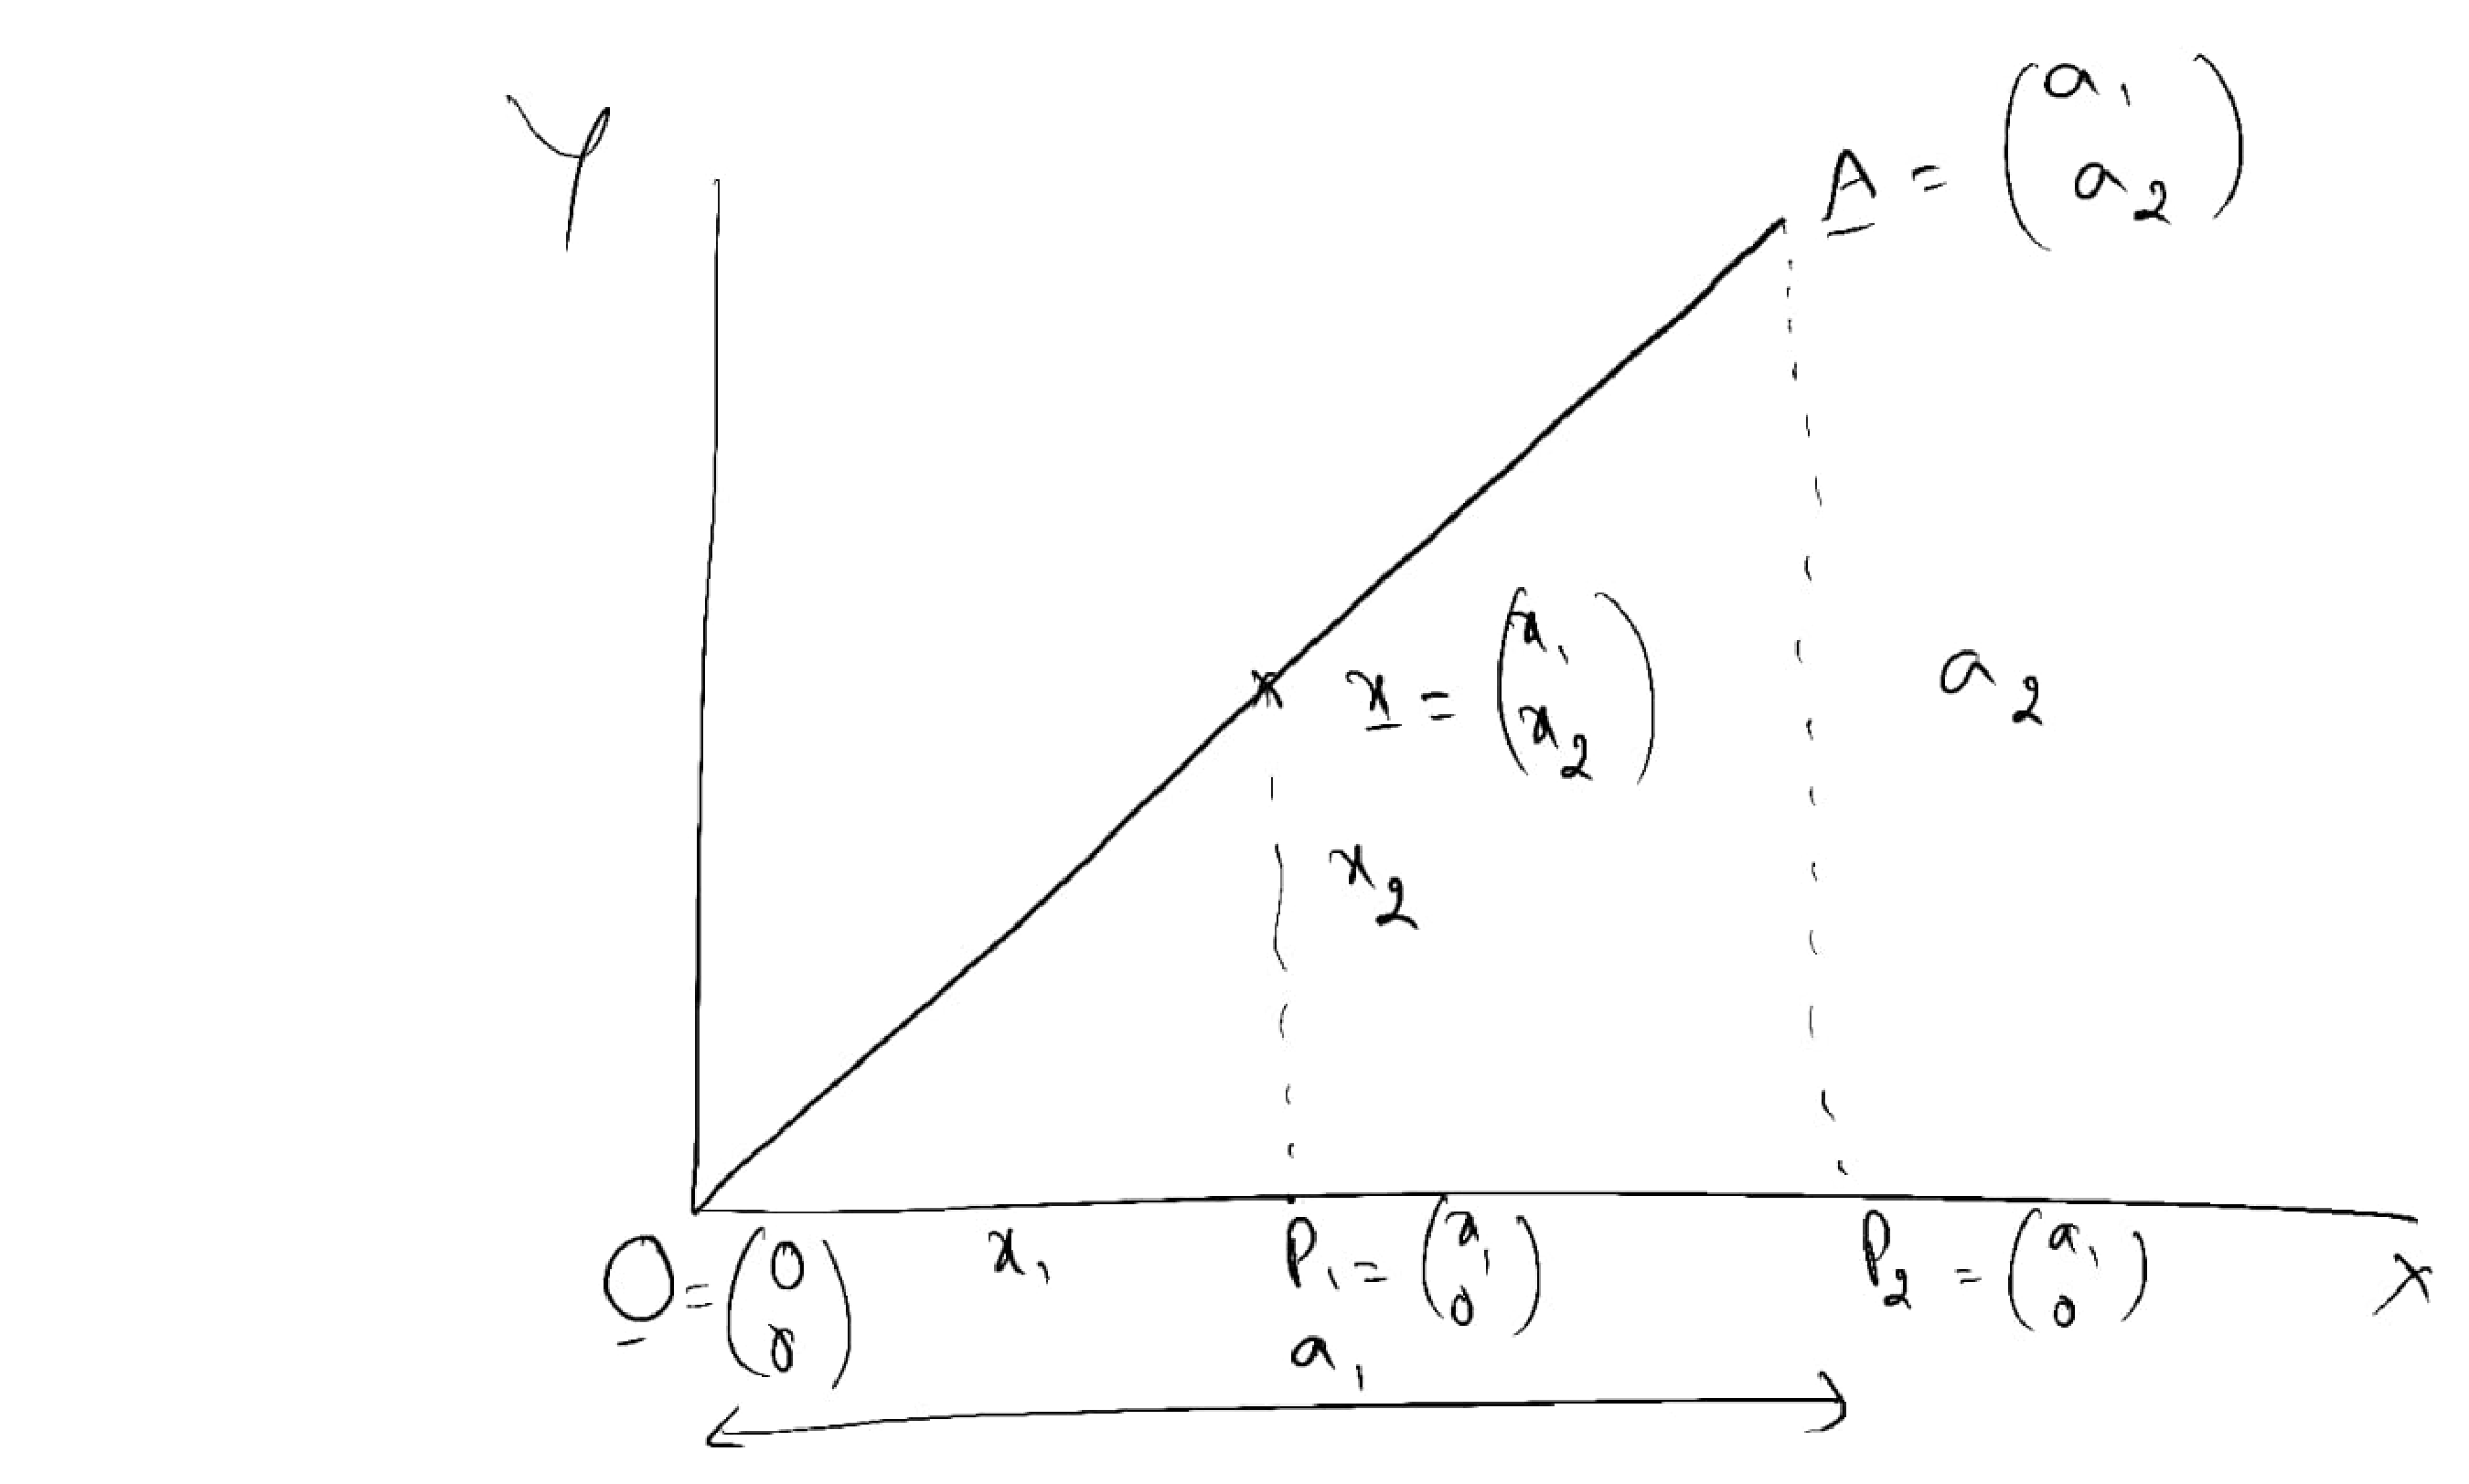
\includegraphics[width=\columnwidth]{./line/figs/line_homog.eps}
\caption{}
\label{fig:line_homog}
\end{figure}
\\
\solution
Let $\vec{x}=\myvec{x_1\\x_2}$ be any point on $OA$.
Then, using similar triangles,
\begin{align}
\frac{x_2}{x_1} &= \frac{a_2}{a_1} = m
\\
\implies x_2 &=  m x_1
\end{align}
where $m$ is known as the slope of the line. Thus, the equation of the line is
\begin{align}
%\label{eq:homog}
\vec{x} = \myvec{x_1\\m x_1} = x_1 \myvec{1 \\ m} = x_1\vec{m}
\end{align}
In general, the above equation is written as
\begin{align}
\label{eq:homog}
\vec{x} = \lambda \vec{m},
\end{align}
%
where $\vec{m}$ is the direction vector of the line.

\item Find the equation of $AB$ in Fig. \ref{fig:line_nhomog}
\begin{figure}
\centering
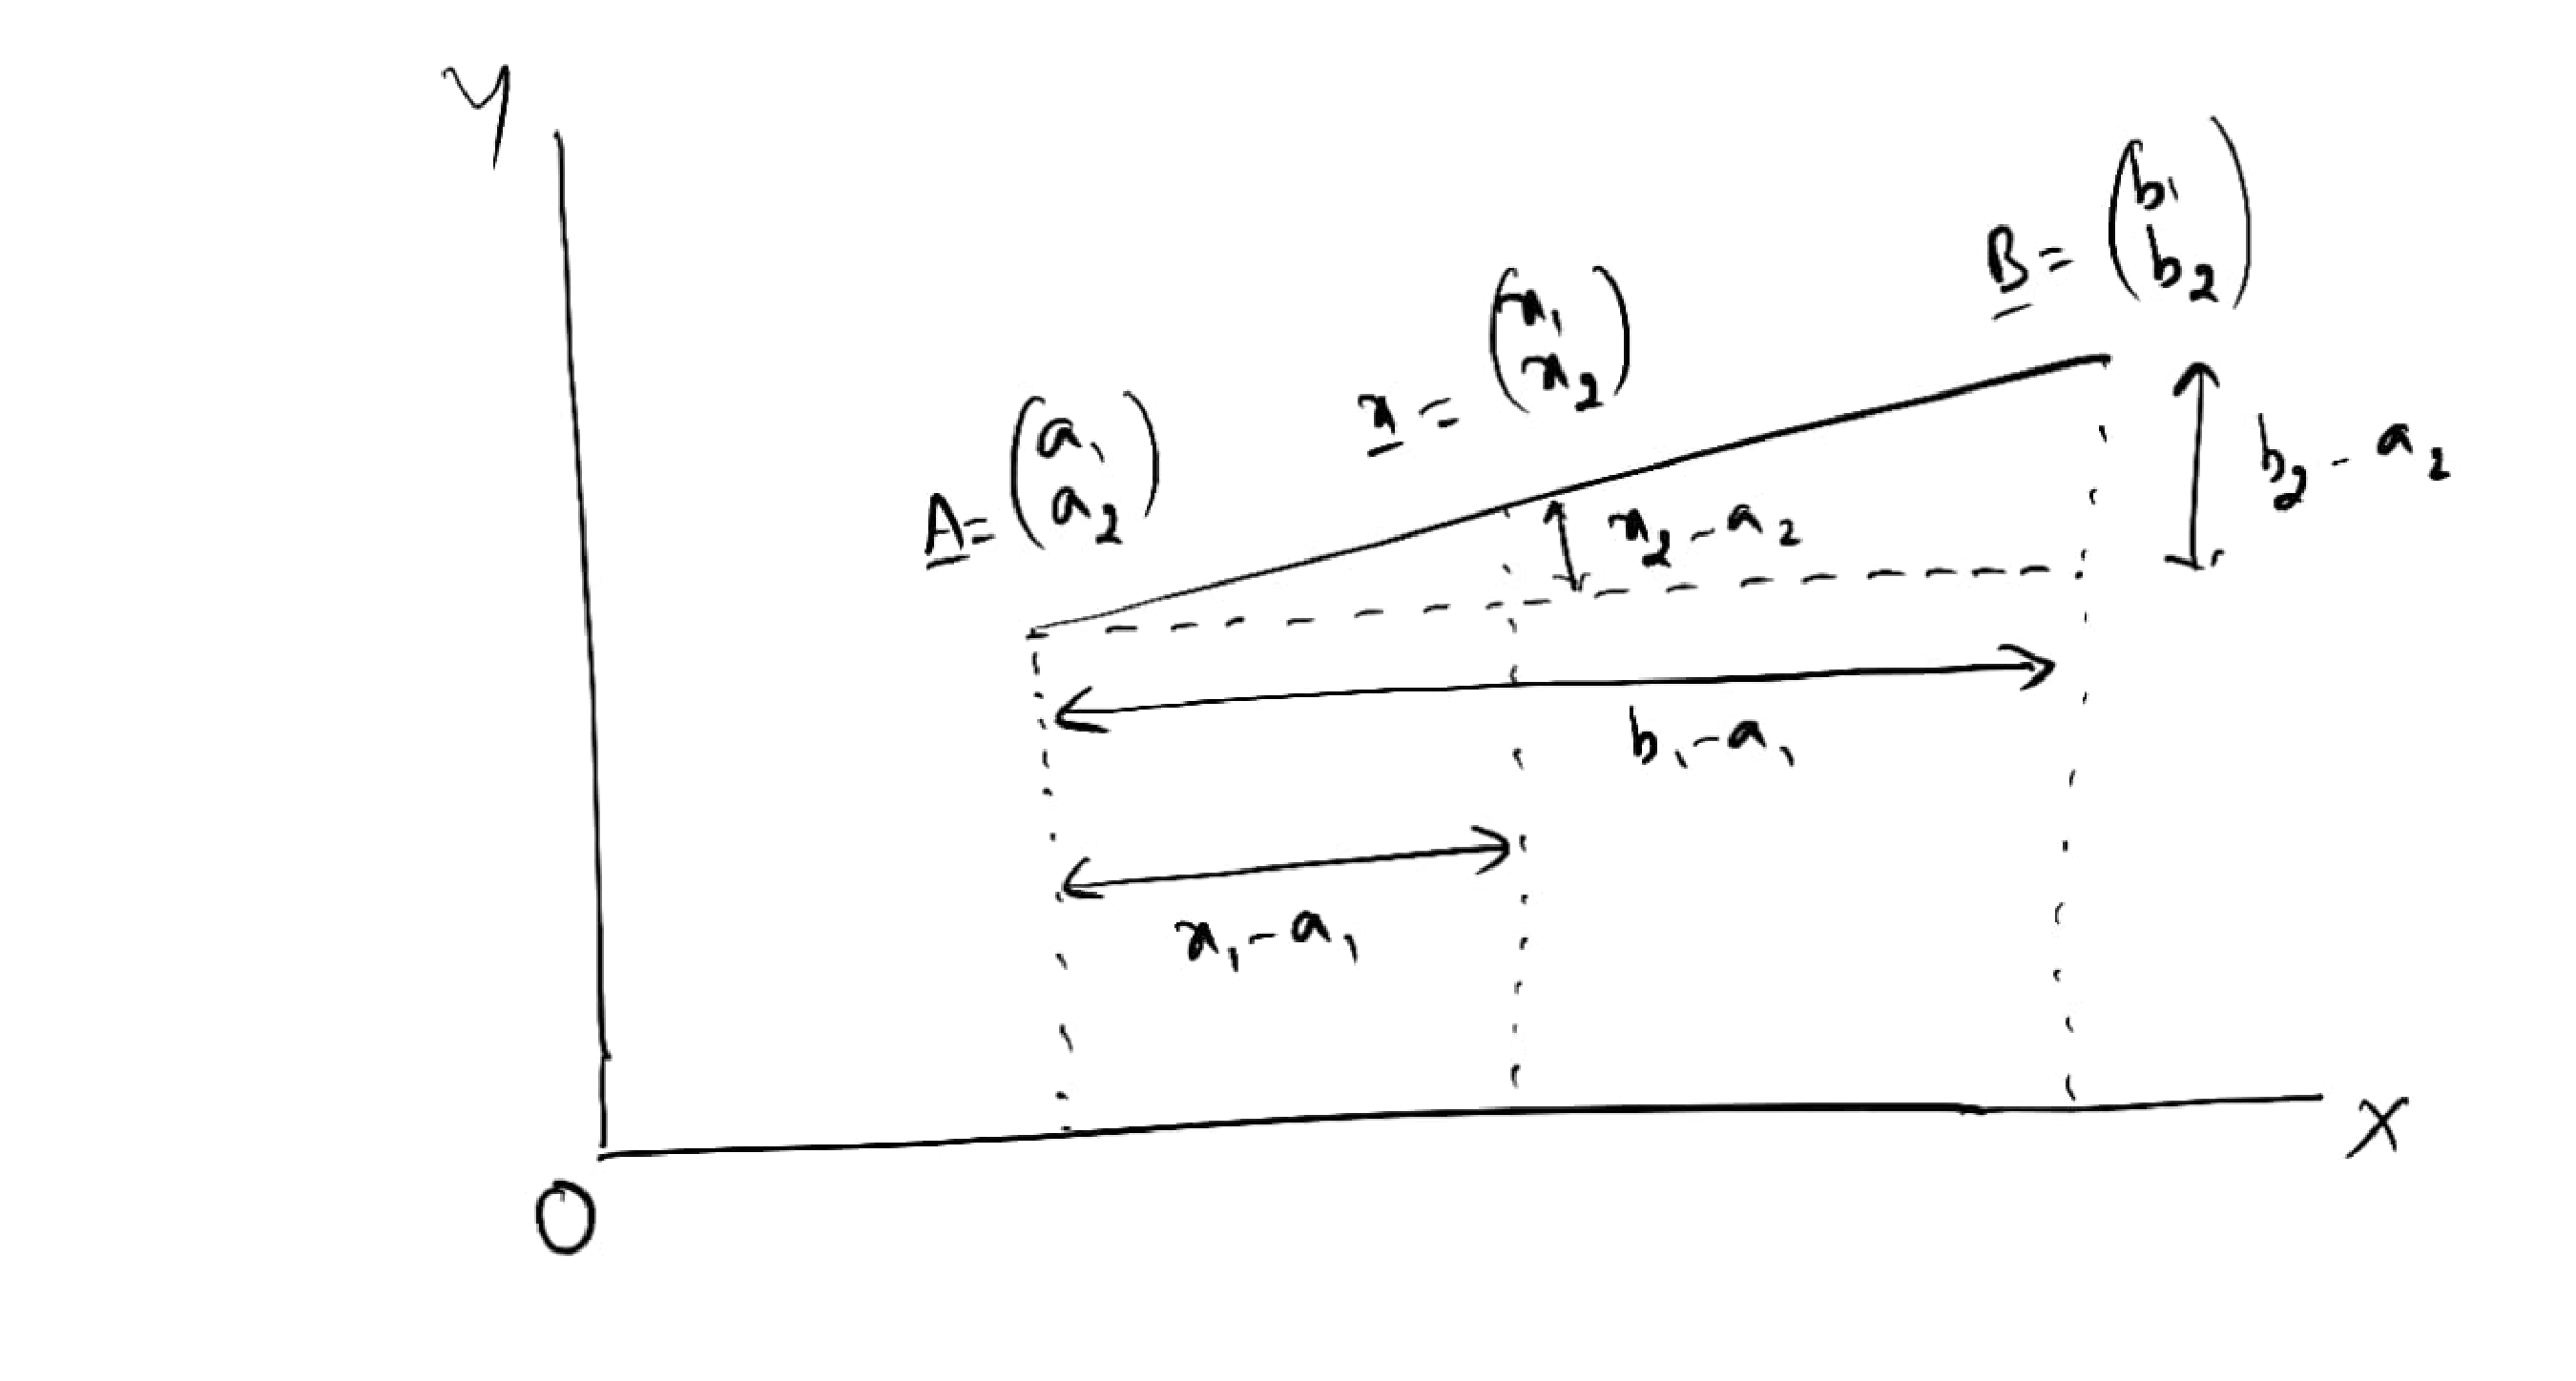
\includegraphics[width=\columnwidth]{./line/figs/line_nhomog.eps}
\caption{}
\label{fig:line_nhomog}
\end{figure}
\\
\solution 
From Fig. \ref{fig:line_nhomog}, 
%
\begin{align}
\frac{x_2-a_2}{x_1-a_1} = \frac{b_2-a_2}{b_1-a_1} = m
\\
\implies x_2 = m x_1 + a_2-ma_1
\label{eq:line_shift}
\end{align}
%
From \eqref{eq:line_shift},
\begin{align}
\myvec{x_1 \\ x_2} &= 
\myvec{x_1 \\   m x_1 + a_2-ma_1
} 
\\
&=\vec{A} + \brak{x_1-a_1}  \myvec{1 \\ m}
\\
&=\vec{A} + \lambda  \vec{m}
\label{eq:nhomog}
\end{align}
\item {\em Translation:} If the line shifts from the origin by $\vec{A}$, \eqref{eq:nhomog} is obtained from \eqref{eq:homog} by adding $\vec{A}$.
\item Find the length of $\vec{A}$ in Fig. \ref{fig:line_homog}
\\
\solution Using Baudhayana's theorem, the length of the vector $\vec{A}$ is defined as
\begin{equation}
 \norm{\vec{A}} = OA = \sqrt{a_1^2 + a_2^2}
=\sqrt{\vec{A}^T\vec{A}}.
\end{equation}
%
Also, from \eqref{eq:homog}, 
\begin{equation}
\norm{\vec{A}} = \lambda \sqrt{1+m^2}
\end{equation}
%
Note that $\lambda$ is the variable that determines the length of $\vec{A}$, 
since $m$ is constant for all points on the line.
%
\item Find $\vec{A}-\vec{B}$.
\begin{figure}
\centering
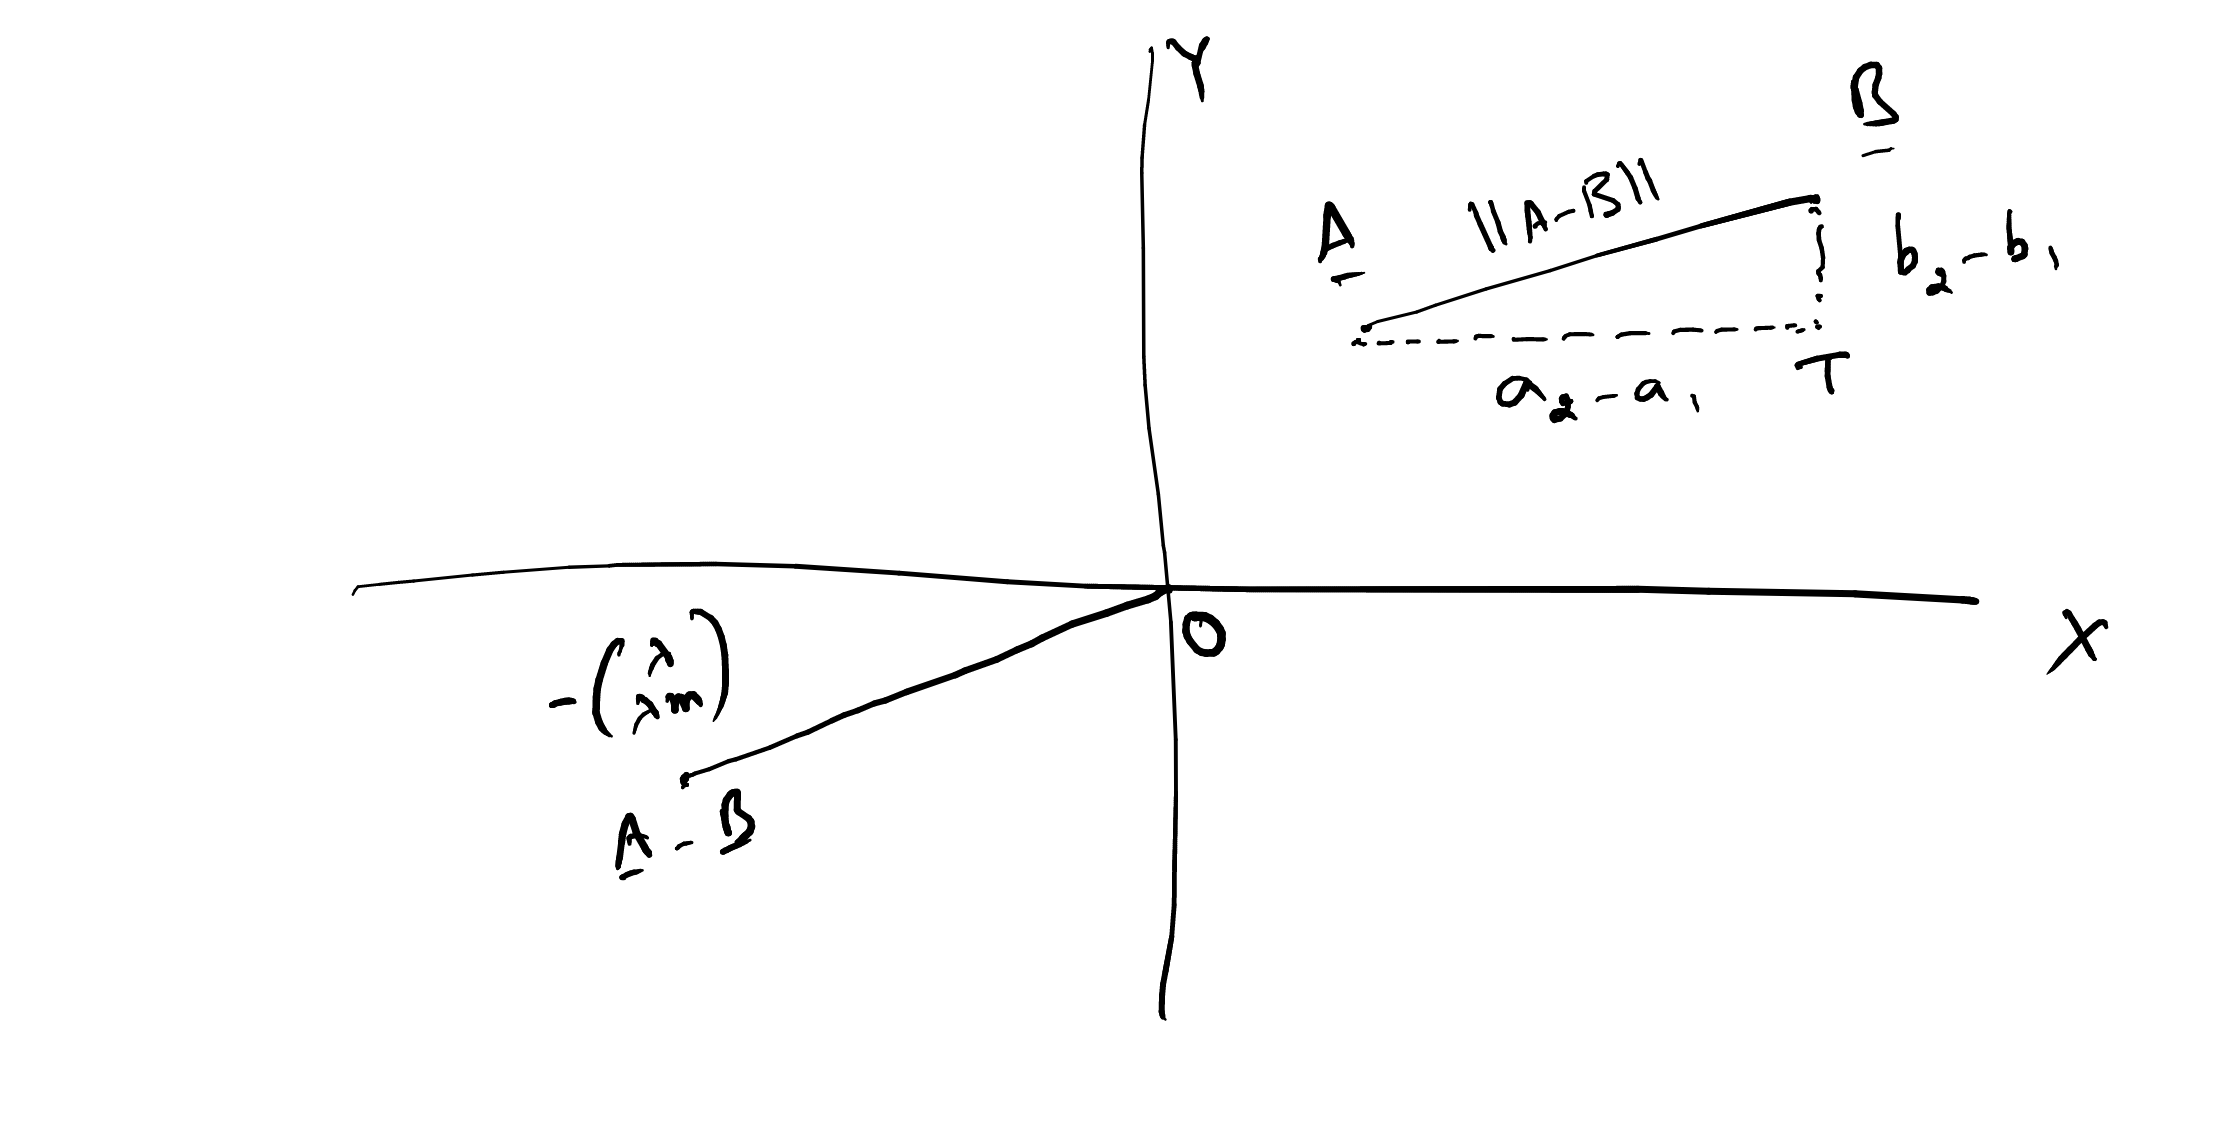
\includegraphics[width=\columnwidth]{./line/figs/ab.eps}
\caption{}
\label{fig:ab}
\end{figure}
%
\\
\solution See Fig. \ref{fig:ab}. From \eqref{eq:nhomog}, for some 
$\lambda$,
\begin{align}
\vec{B} &=\vec{A} + \lambda \myvec{1 \\ m}
\\
\implies \vec{A} - \vec{B} &= - \lambda \myvec{1 \\ m},
\end{align}
%
$\vec{A} - \vec{B}$ is marked in Fig. \ref{fig:ab}.
%
\item Show that $AB = \norm{\vec{A}-\vec{B}}$
\item Show that the equation of $AB$ is
\begin{align}
\label{eq:line_ab}
\vec{x} = \vec{A}+ \lambda\brak{\vec{B}-\vec{A}}
\end{align}
%
\item The {\em normal} to the vector $\vec{m}$ is defined as
\begin{align}
\label{eq:normal}
\vec{n}^T\vec{m} = 0
\end{align}
\begin{align}
\label{eq:normal_omat}
\vec{n} = \myvec{0 & 1\\ -1 & 0}\vec{m}
\end{align}
\item From \eqref{eq:line_ab}, the equation of a line can also be expressed as
\begin{align}
\label{eq:line_ab_normal}
\vec{n}^T\vec{x} &= \vec{n}^T\vec{A}+ \lambda\vec{n}^T\brak{\vec{B}-\vec{A}}
\\
\implies \vec{n}^T\vec{x} &=\vec{n}^T\vec{A}=c
\label{eq:line_normal}
\end{align}
\item The unit vectors on the $x$ and $y$ axis are defined as
\begin{align}
\label{eq:line_unit}
\vec{e}_1 &=\myvec{1\\0}, 
\\
\vec{e}_2 &=\myvec{0\\1}
\end{align}
\item If $a$ be the {\em intercept} of the line 
\begin{align}
\label{eq:line_intercept}
\vec{n}^T\vec{x} &=c
\end{align}
on the $x-$axis, then $\myvec{a\\0}$  is a point on the line.  Thus, 
\begin{align}
%\label{eq:line_intercept}
\vec{n}^T\myvec{a\\0} &=c
\\
\implies a &= \frac{c}{\vec{n}^T\vec{e}_1}
\end{align}
%
\renewcommand{\theequation}{\theenumi}
%
\item The {\em rotation matrix} is defined as
\begin{align}
\vec{Q} = \myvec{\cos \theta & -\sin \theta\\ \sin \theta & \cos \theta}
\end{align}
%
where $\theta$ is anti-clockwise.
\item 
\begin{align}
\vec{Q}^T\vec{Q} = \myvec{1 & 0 \\ 0 & 1} = \vec{I}
\end{align}
%
where $\vec{I}$ is the {\em identity matrix}. The rotation matrix $\vec{Q}$ is also an {\em orthogonal matrix}.

\numberwithin{equation}{enumi}
%
\item Find the equation of  line $L$ in Fig. \ref{fig:line_dist}.
\\
\solution The equation of the $x-$axis is
\begin{align}
\vec{x} =\lambda \vec{e}_1
\end{align}
Translation by $p$ units along the $y-$axis results in 
\begin{align}
L_0: \quad \vec{x} = \lambda \vec{e}_1 + p \vec{e}_2 
\end{align}
Rotation by $90\degree-\alpha$ in the anti-clockwise direction yields
\begin{align}
L: \quad \vec{x} &= \vec{Q}\cbrak{\lambda \vec{e}_1 + p \vec{e}_2 }
\\
&=\lambda \vec{Q}\vec{e}_1 + p \vec{Q}\vec{e}_2 
\label{eq:line_dist_temp}
\end{align}
%
where 
\begin{align}
\vec{Q} &= \myvec{\cos \brak{\alpha-90} & -\sin \brak{\alpha-90}\\ \sin \brak{\alpha-90} & \cos \brak{\alpha-90}}
\\
&= \myvec{\sin \alpha & \cos \alpha \\ -\cos \alpha & \sin \alpha}
\end{align}
%
From \eqref{eq:line_dist_temp},
\begin{align}
L: \quad \vec{e}_2^T\vec{Q}^T\vec{x}&=\lambda \vec{e}_2^T\vec{Q}^T\vec{Q}\vec{e}_1 + p \vec{e}_2^T\vec{Q}^T\vec{Q}\vec{e}_2 
\nonumber \\
&=\lambda \vec{e}_2^T\vec{e}_1 + p \vec{e}_2^T\vec{e}_2 
\end{align}
resulting in 
\begin{align}
L: \quad \myvec{\cos \alpha & \sin \alpha}\vec{x}=p
\label{eq:line_dist_temp_final}
\end{align}
\begin{figure}
\centering
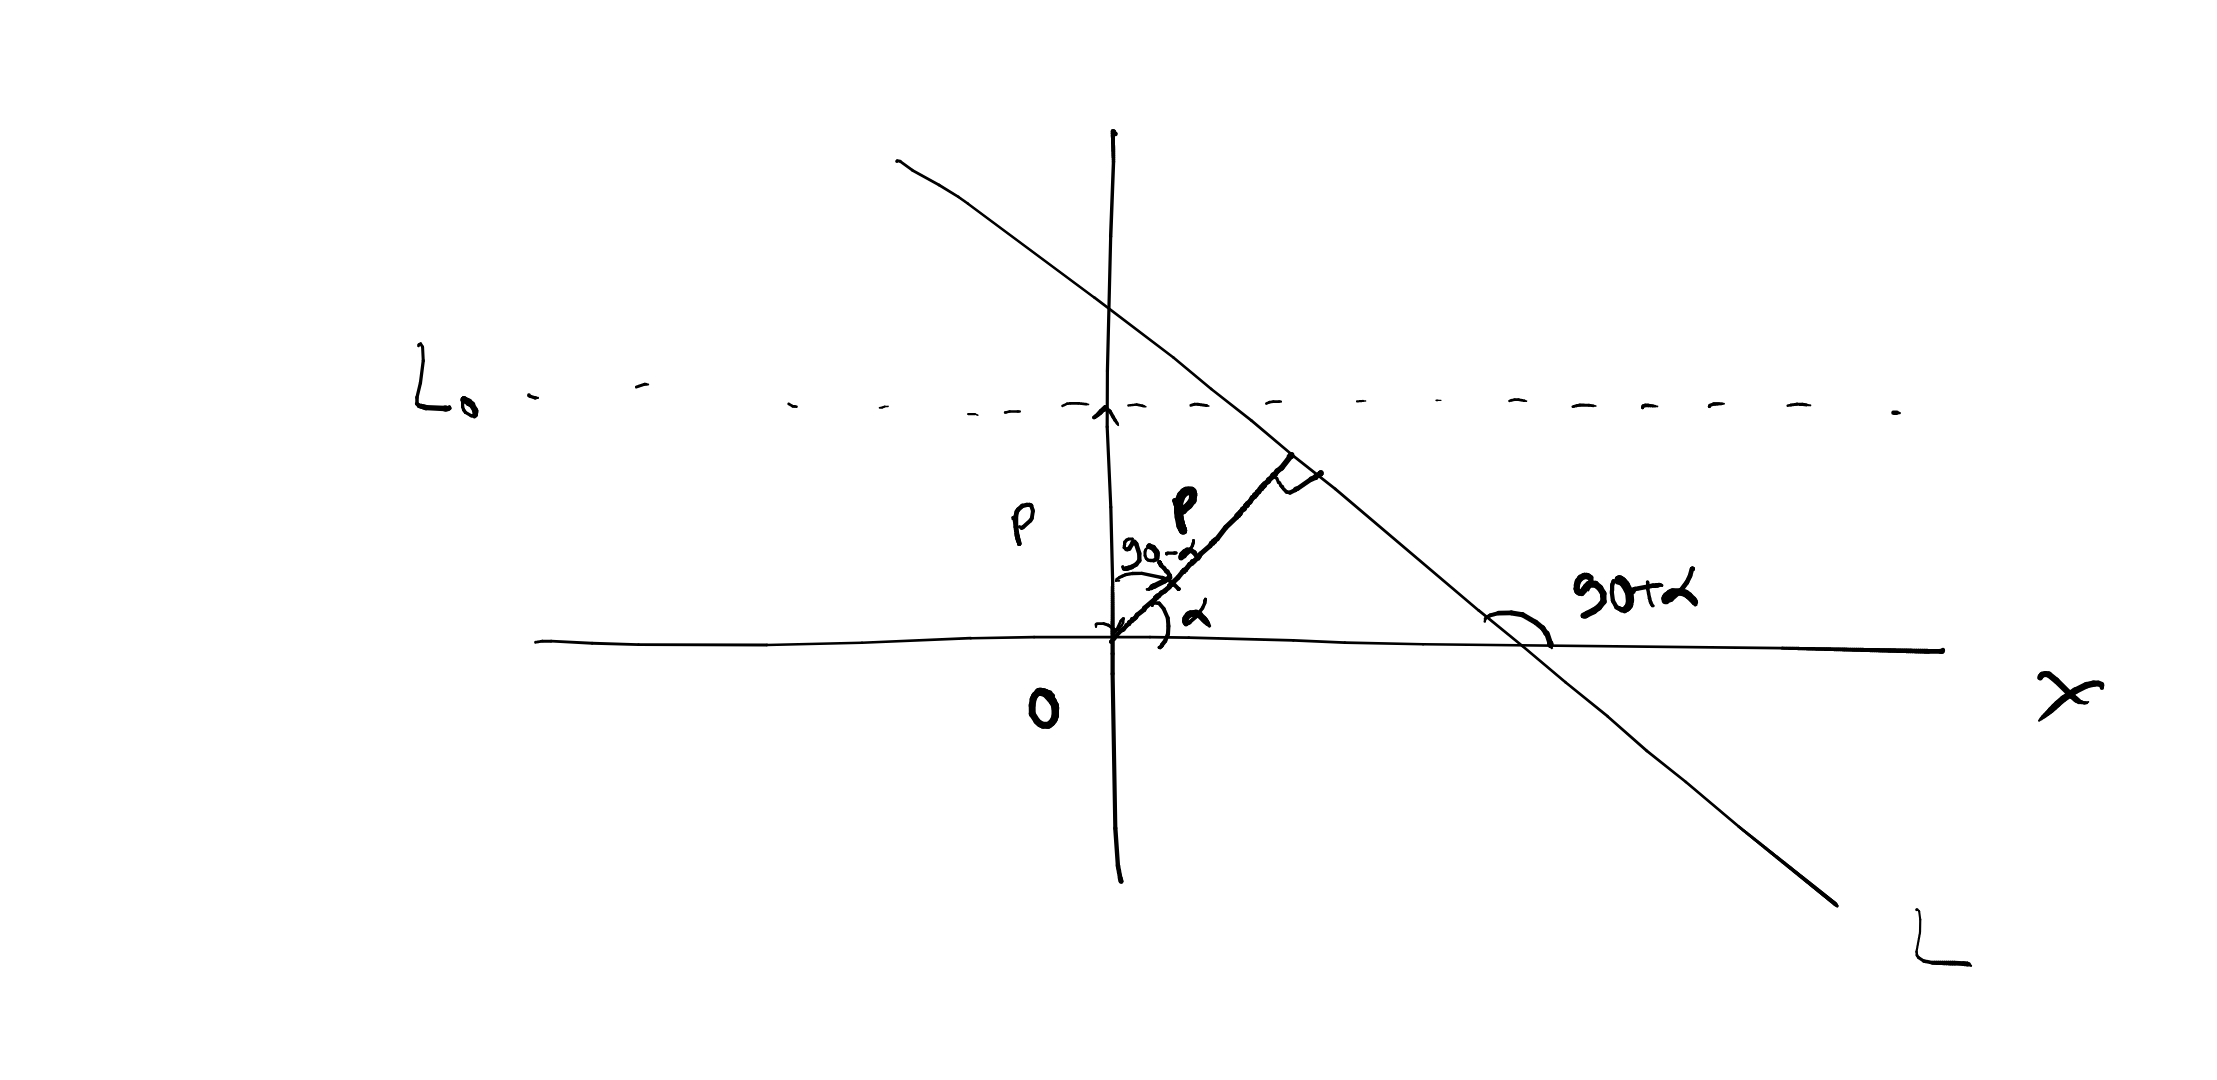
\includegraphics[width=\columnwidth]{./line/figs/line_dist.eps}
\caption{}
\label{fig:line_dist}
\end{figure}
\item Show that the distance from the orgin to the line 
\begin{align}
\vec{n}^T\vec{x} &=c
\end{align}
is 
\begin{align}
p = \frac{c}{\norm{n}}
\label{eq:line_dist_orig}
\end{align}
\item Show that the point of intersection of two lines 
\begin{align}
\vec{n}_1^T\vec{x} &=c_1
\\
\vec{n}_2^T\vec{x} &=c_2
\end{align}
is given by 
\begin{align}
\label{eq:line_intersection}
\vec{x} &=\brak{\vec{N}^T}^{-1}\vec{c}
\end{align}
where 
\begin{align}
\vec{N} = \myvec{\vec{n}_1 & \vec{n}_2}
\end{align}
\item The {\em angle between two lines} is given by 
\begin{align}
\cos ^{-1} \frac{\vec{n}_1 ^T \vec{n}_2}{\norm{\vec{n}_1}  \norm{\vec{n}_2}}
\end{align}
\item Show that the distance of a point $\vec{x}_0$ from the line 
\begin{align}
L: \quad \vec{n}^T\vec{x} &=c
\end{align}
is 
\begin{align}
\frac{\abs{\vec{n}^T\vec{x}_0-c}}{\norm{\vec{n}}} 
\label{eq:line_dist_pt}
\end{align}
\solution Let the equation of the line be 
\begin{align}
\vec{x} = \vec{A} + \lambda \vec{m}
\end{align}
%
where 
\begin{align}
\label{eq:line_dist_orig_pt}
\vec{n}^T\vec{A} = c, \vec{n}^T\vec{m} = 0
\end{align}
If $\vec{x}_0$ is translated to the origin, the equation of the line $L$ becomes 
\begin{align}
\vec{x} &= \vec{A}- \vec{x}_0+ \lambda \vec{m}
\\
\implies 
\vec{n}^T\vec{x} &=c-\vec{n}^T\vec{x}_0
\end{align}
From \eqref{eq:line_dist_orig}, \eqref{eq:line_dist_orig_pt} is obtained.
\item Show that 
\begin{align}
ax^2+2bxy+cy^2+2dx+2ey+f=0
\end{align}
can be expressed as
\begin{align}
\label{eq:quad_form}
\vec{x}^T\vec{V}\vec{x}+2\vec{u}^T\vec{x}+f=0
\end{align}
%
where
\begin{align}
\vec{V} &= \vec{V}^T
\\
\vec{u} &= \myvec{d & e}
\end{align}

\item {\em Pair of straight lines:} \eqref{eq:quad_form}
%The equation
%\begin{align}
%\vec{x}^T\myvec{a & b\\ b & c}\vec{x}+2\myvec{d & e}+f=0
%\end{align}
%
represents a pair of straight lines if 
\begin{align}
\begin{vmatrix}
\vec{V}&\vec{u}
\\
\vec{u}^T&f
\end{vmatrix}
= 0
\end{align}
%
Two intersecting lines are obtained if 
\begin{align}
\abs{\vec{V}} < 0
\end{align}
\item  In Fig. \ref{fig:ratio}, let
\begin{equation}
\frac{AB}{BC} = \frac{\norm{\vec{A}-\vec{B}}}{\norm{\vec{B}-\vec{C}}} = k.
\label{eq:k}
\end{equation}
%
Show that
\begin{equation}
\frac{\vec{A}+k\vec{C}}{k+1} = \vec{B}.
\label{eq:ratio}
\end{equation}
%
\solution
%
\begin{figure}[!hb]
\centering
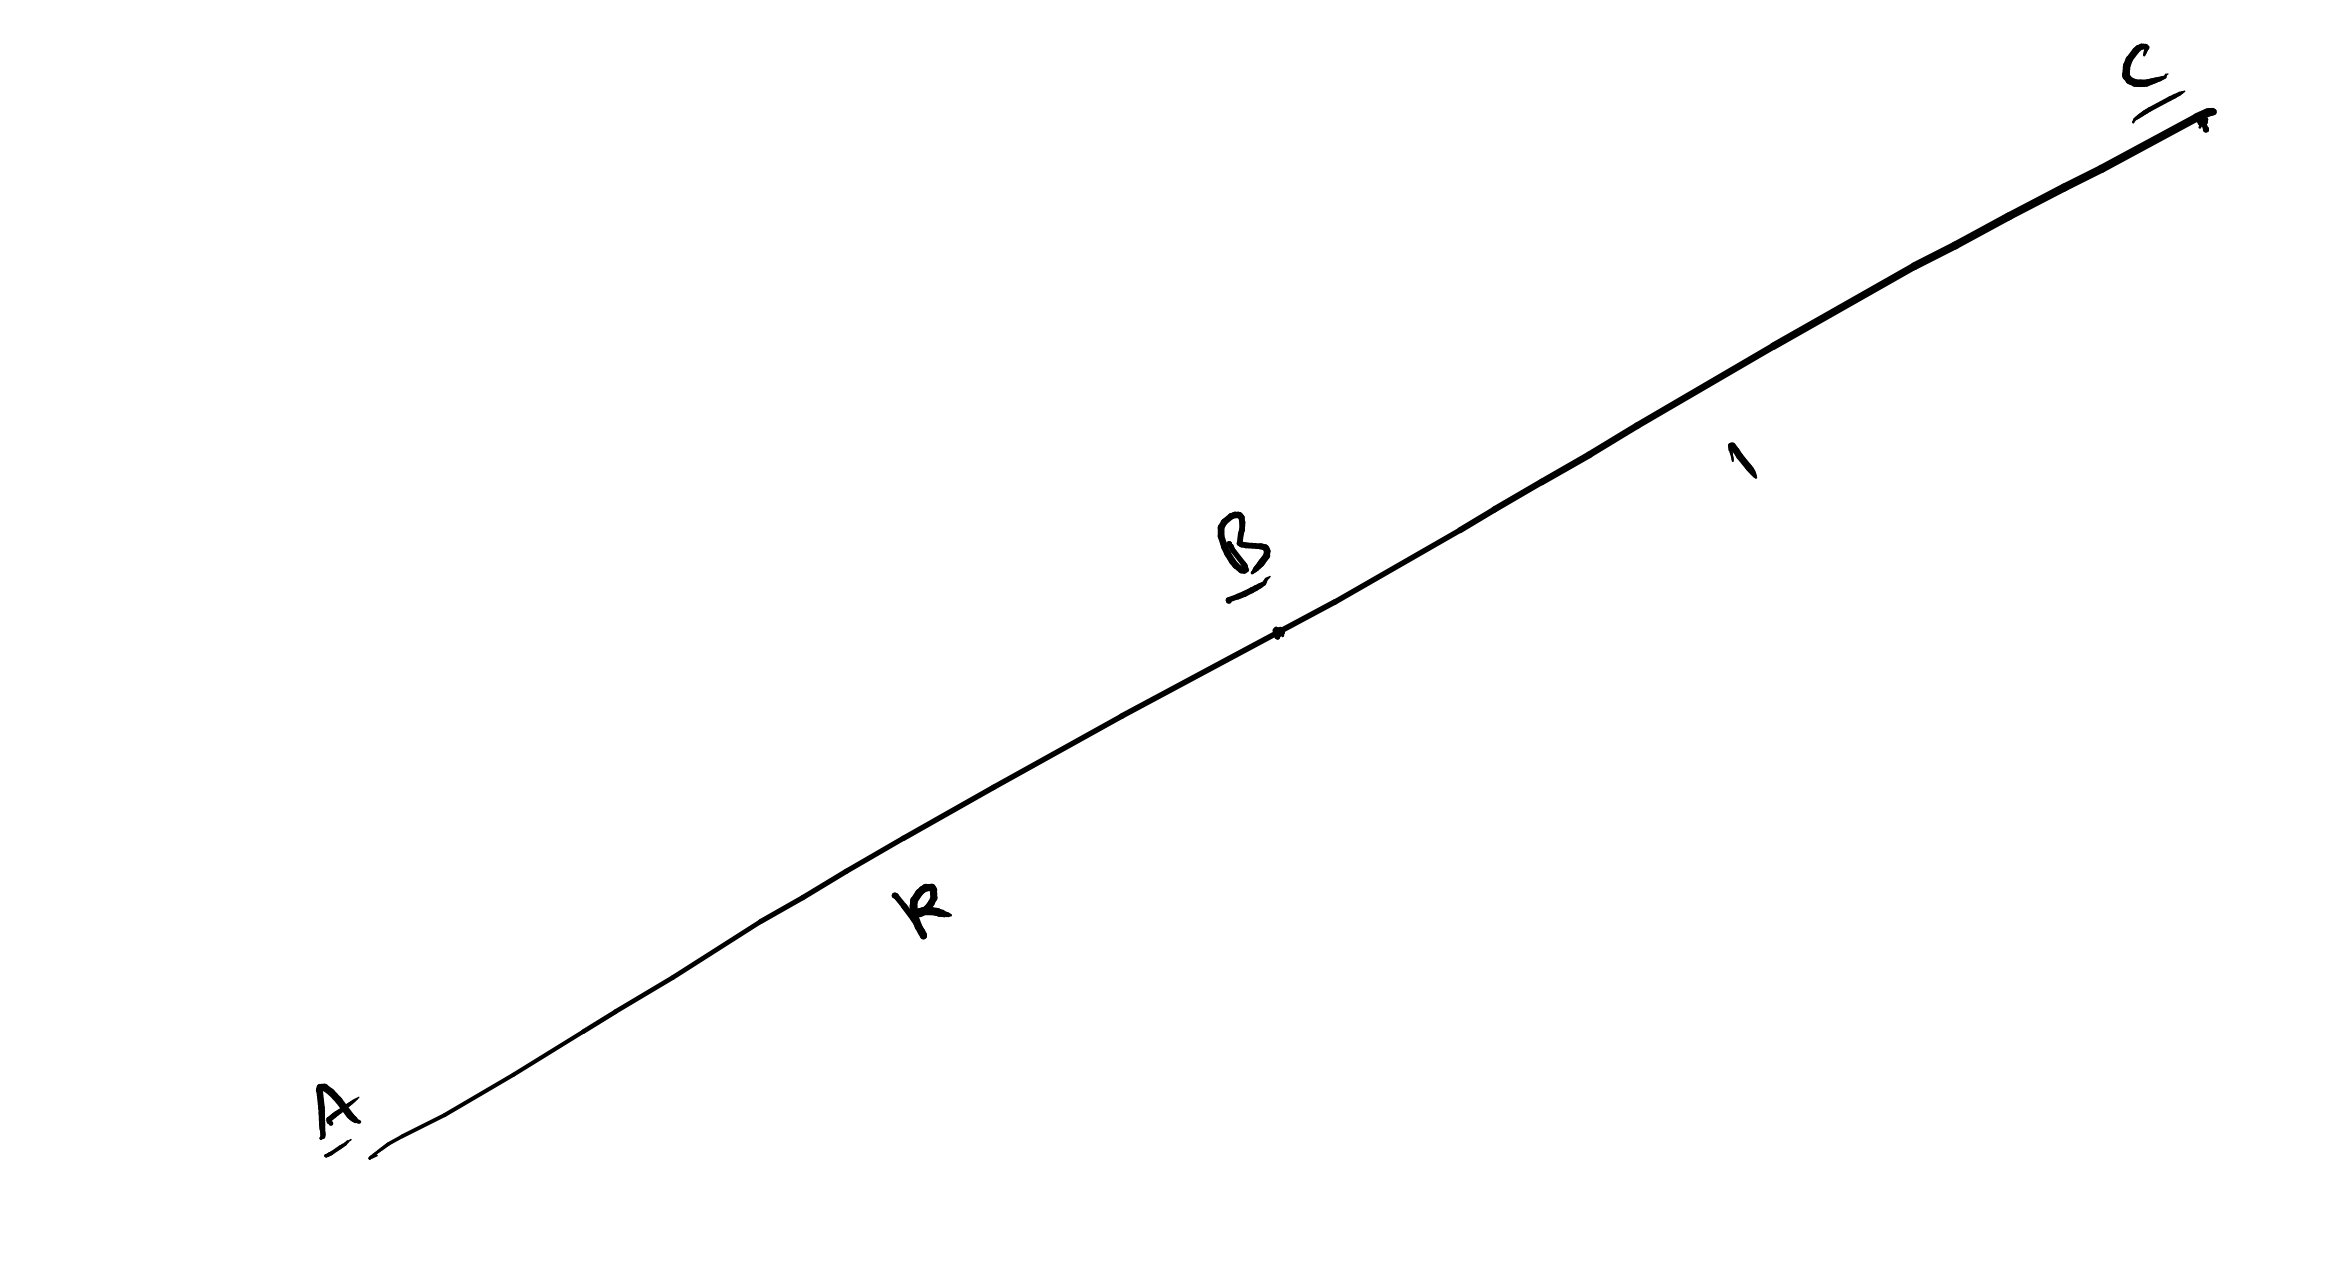
\includegraphics[width=\columnwidth]{./line/figs/ratio.eps}
\caption{}
\label{fig:ratio}
\end{figure}
From \eqref{eq:nhomog}, 
\begin{align}
\begin{split}
\vec{B} &= \vec{A} + \lambda_1 \vec{m}
\\
\vec{B} &= \vec{C} - \lambda_2 \vec{m}
\end{split}
\\
\label{eq:rat_1}
\implies \frac{\norm{\vec{A}-\vec{B}}}{\norm{\vec{B}-\vec{C}}} &= 
\frac{\lambda_1}{\lambda_2} = k
\\
\text{and } \frac{\vec{B}- \vec{A}}{\lambda_1} &= \frac{\vec{C}- 
\vec{B}}{\lambda_2} = \vec{m},
\label{eq:rat_2}
\end{align}
%
from \eqref{eq:k}. Using \eqref{eq:rat_1} and \eqref{eq:rat_2},
\begin{align}
\vec{A}- \vec{B} &=  k\brak{\vec{B}- \vec{C}}
\end{align}
%
resulting in \eqref{eq:ratio}

%
\item If $\vec{A}$ and $\vec{B}$ are linearly independent,  
\begin{equation}
k_1\vec{A} + k_2\vec{B} = 0 \implies k_1=k_2=0
\end{equation}
\item Show that $\vec{D}$ lies inside $\triangle ABC$ iff
\begin{align}
\vec{D} = \lambda_1\vec{A} + \lambda_2\vec{B} + \lambda_3\vec{C}
\end{align}
such that
\begin{align}
0 \le \lambda_1, \lambda_2, \lambda_3 &\le 1,
\\
0 \le \lambda_1+\lambda_2+\lambda_3 &\le 1,
\end{align}
%\item Show that if 
%\begin{align}
%\vec{m}_1 + k\vec{m}_2 \ne 0,
%\end{align}
%%
%there exists $k$ such that for any point $\vec{m}$,
%\begin{align}
%\label{eq:line_basis}
%\vec{m} = \vec{m}_1 + k\vec{m}_2 
%\end{align}
\item
In $\Delta ABC$,  Let $\vec{P}$ be a point on $BC$ such that $AP \perp BC$.  Then $AP$ is defined to be 
an {\em altitude} of $\Delta ABC$.

\item
\label{prob:alt_eq}
Find the intersection of $AP$ and $BQ$.
\\
\solution The normal vector of $AP$ is $\vec{B} - \vec{C}$. From \eqref{eq:normal}
and \eqref{eq:line_normal},
%\eqref{eq:line_norm}
 the equation of $AP$ and $BQ$ are
\begin{align}
\label{eq:alt_ap}
\brak{\vec{B} - \vec{C}}^T\brak{\vec{x} - \vec{A}}&= 0
\\
\label{eq:alt_bq}
\brak{\vec{C} - \vec{A}}^T\brak{\vec{x} - \vec{B}}&= 0
%\\
%\implies \myvec{-3&4}\vec{x} = -\myvec{-3&4}\myvec{2\\2} &= -2
\end{align}
which can be solved to obtain the intersection point using \eqref{eq:line_intersection}.
\item Show that the equation of the angle bisectors of the lines
\begin{align}
\vec{n}_1^T\vec{x} &=c_1
\\
\vec{n}_2^T\vec{x} &=c_2
\end{align}
%
is
\begin{align}
\frac{\vec{n}_1^T\vec{x}-c_1}{\norm{\vec{n}_1}}=\pm\frac{\vec{n}_2^T\vec{x} -c_2}{\norm{\vec{n}_2}}\end{align}
\item Find the equation of a line passing through the intersection of the lines
\begin{align}
\label{eq:line1}
\vec{n}_1^T\vec{x} &=c_1
\\
\vec{n}_2^T\vec{x} &=c_2
\label{eq:line2}
\end{align}
and passing through the point $\vec{p}$.
\\
\solution 
%Let the equation of any line through the intersection of \eqref{eq:line1} and \eqref{eq:line2} be 
%\begin{align}
%\vec{n}^T\vec{x} &=c
%\label{eq:line12}
%\end{align}
%
%If $\vec{u}$ be the point of intersection, 
%\begin{align}
%\myvec{\vec{n}_1^T\\ \vec{n}_2^T\\ \vec{n}^T}\vec{u} &= \myvec{c_1\\c_2\\c}
%\\
%\implies \myvec{\vec{n}_1^T & c_1\\ \vec{n}_2^T & c_2\\ \vec{n}^T & c}&
%\label{eq:line12_mat}
%\end{align}
%has rank 2.  Thus, 
%%
%\begin{align}
%\label{eq:line_basis_normal}
%\myvec{\vec{n}\\c} &= k_1\myvec{\vec{n}_1 \\ c_1}+ k_2\myvec{\vec{n}_2\\c_2} 
%\end{align}
%Substituting in \eqref{eq:line12},
%\begin{align}
%\vec{n}^T\vec{x} = c &
%\implies \vec{n}_1^T\vec{x} + k\vec{n}_2^T\vec{x} =  c_1+kc_2=c
%\label{eq:line_basis_normal_temp}
%\end{align}
%%
%Thus, 
%\begin{align}
%k = \frac{\vec{n}_1^T\vec{p}-c_1}{\vec{n}_2^T\vec{p}-c_2}
%\end{align}
%%
%which can be used to obtain the desired equation using \eqref{eq:line_basis_normal_temp}
%
%Alternatively, 
%
%
The intersection of the lines is 
\begin{align}
\vec{x} = \vec{N}^{-T}\vec{c}
\end{align}
%
where 
\begin{align}
\vec{N} &= \myvec{\vec{n}_1 &\vec{n}_2}
\\
\vec{c} &= \myvec{c_1 \\ c_2} 
\end{align}
Thus, the equation of the desired line is 
\begin{align}
\vec{x} = \vec{p}+ \lambda\brak{\vec{N}^{-T}\vec{c}-\vec{p}}&
\\
\implies \vec{N}^{T}\vec{x} = \vec{N}^{T}\vec{p}+ \lambda\brak{\vec{c}-\vec{N}^{T}\vec{p}}&
\end{align}
resulting in 
\begin{multline}
 \brak{\vec{c}-\vec{N}^T\vec{p}}^T\myvec{0 & -1 \\ 1 & 0}\vec{N}^T\vec{x} 
\\
= \brak{\vec{c}-\vec{N}^T\vec{p}}^T\myvec{0 & -1 \\ 1 & 0}\vec{N}^T\vec{p}
\end{multline}
\item Find $\vec{R}$, the {\em reflection}  of $\vec{P}$ about the line
\begin{align}
L: \quad \vec{n}^T\vec{x} = c
\end{align}
%
\begin{figure}
\centering
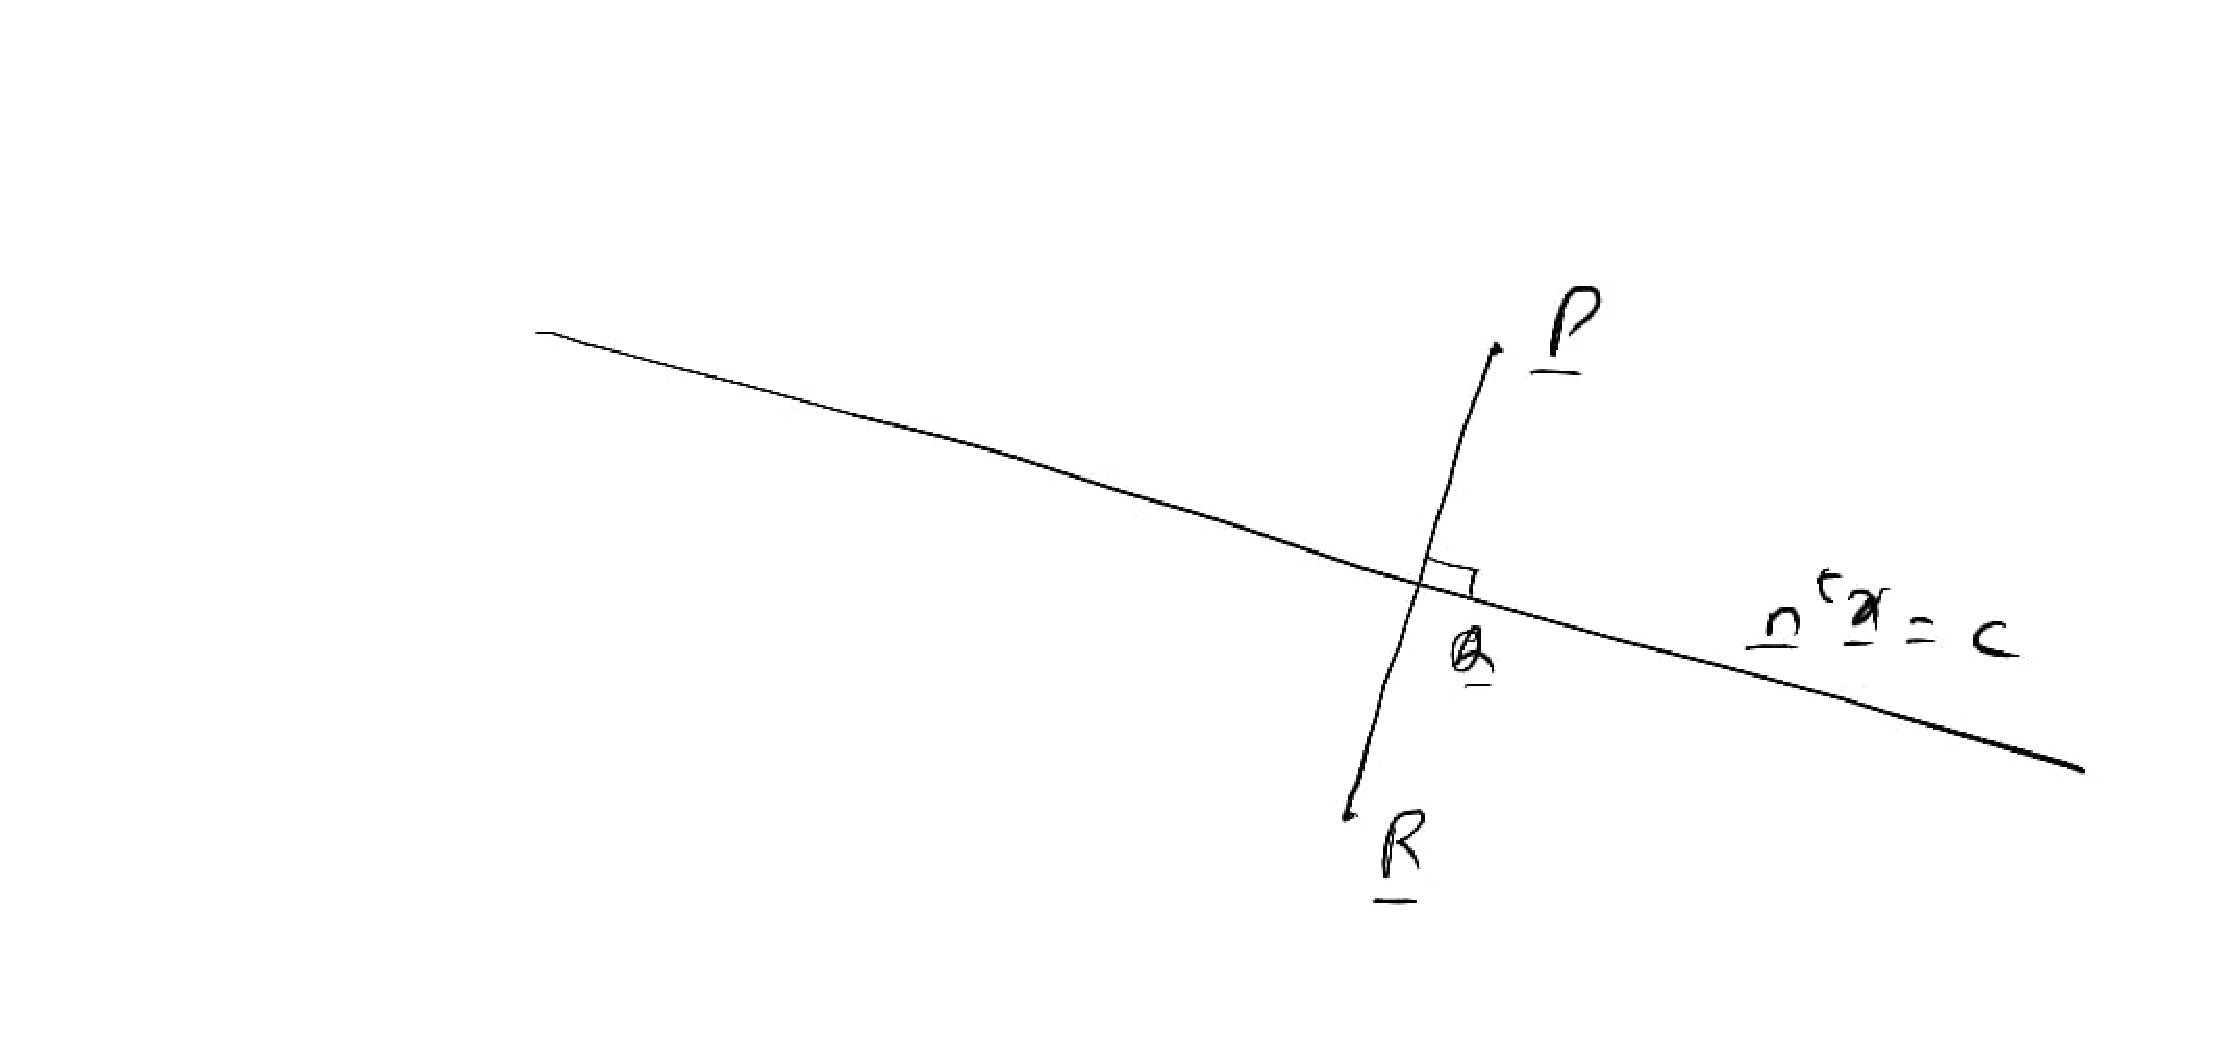
\includegraphics[width=\columnwidth]{./line/figs/reflection.eps}
\caption{}
\label{fig:locus}
\end{figure}
\solution Since $\vec{R}$ is the reflection of $\vec{P}$ and $\vec{Q}$ lies on $L$, $\vec{Q}$ bisects $PR$.  
This leads to the following equations
Hence, 
\begin{align}
\label{eq:reflect_bisect}
2\vec{Q} &= \vec{P}+\vec{R}
\\
\label{eq:reflect_Q}
\vec{n}^{T}\vec{Q} &= c
\\
\label{eq:reflect_R}
\vec{m}^{T}\vec{R} &= \vec{m}^{T}\vec{P}
\end{align}
%
where $\vec{m}$ is the direction vector of $L$.  From \eqref{eq:reflect_bisect} and \eqref{eq:reflect_Q},
\begin{align}
\label{eq:reflect_bisectQ}
\vec{n}^{T}\vec{R}  &= 2c - \vec{n}^{T}\vec{P}
\end{align}
%
From \eqref{eq:reflect_bisectQ} and \eqref{eq:reflect_R},
\begin{align}
\label{eq:reflect_bisectQR}
\myvec{\vec{m} & \vec{n}}^T\vec{R} &= \myvec{\vec{m} & -\vec{n}}^T\vec{P}+ \myvec{0 \\ 2c}
\end{align}
%
Letting 
\begin{align}
\label{eq:reflect_mat}
\vec{V}=  \myvec{\vec{m} & \vec{n}}
\end{align}
with the condition that $\vec{m},\vec{n}$ are orthonormal, i.e.
\begin{align}
\label{eq:reflect_ortho}
\vec{V}^T\vec{V}=  \vec{I}
\end{align}
%
Noting that 
\begin{align}
\label{eq:reflect_trans}
\myvec{\vec{m} & -\vec{n}} &= \myvec{\vec{m} & \vec{n}} \myvec{1 & 0 \\ 0 & -1},
\end{align}
\eqref{eq:reflect_bisectQR} can be expressed as
%
\begin{align}
\label{eq:reflect_}
\vec{V}^T\vec{R} &=  \sbrak{\vec{V}\myvec{1 & 0 \\ 0 & -1}}^T\vec{P}+\myvec{0 \\ 2c}
\\
\implies \vec{R} &= \sbrak{\vec{V}\myvec{1 & 0 \\ 0 & -1}\vec{V}^{-1}}^T\vec{P}+ \vec{V}\myvec{0 \\ 2c}
\\
 &=\vec{V}\myvec{1 & 0 \\ 0 & -1}\vec{V}^T \vec{P}+2c \vec{n}
\end{align}
\item Show that, for any $\vec{m},\vec{n}$, the reflection is also given by
\begin{align}
%\label{eq:reflect_bisect}
\frac{\vec{R}}{2} = \frac{\vec{m}\vec{m}^T-\vec{n}\vec{n}^T}{\vec{m}^T\vec{m}+\vec{n}^T\vec{n}}\vec{P} + c 
\frac{\vec{n}}{\norm{\vec{n}}^2}
\end{align}

\end{enumerate}
%
%
%\item Let $\vec{x}$ be any point on $AB$ in Fi.g \ref{fig:orth}.  Show that
%\begin{equation}
%\brak{\vec{x}-\vec{A}}^T\brak{\vec{B}-\vec{C}} = 0
%\end{equation}
%%
%\item If $\vec{x,y}$ are any two points on $AB$, show that 
%\begin{equation}
%\label{eq:orth_any}
%\brak{\vec{x}-\vec{y}}^T\brak{\vec{B}-\vec{C}} = 0
%\end{equation}
%%
%\item In Fig. \ref{fig:alt}, $BE \perp AC, CF \perp AB$.  Show that $AD \perp BC$.
%\begin{figure}[!hb]
%\centering
%\includegraphics[width=\columnwidth]{./figs/alt.eps}
%\caption{}
%\label{fig:alt}
%\end{figure}
%\\
%\solution Let $\vec{x}$ be the intersection of $BE$ and $CF$. Then, using 
%\eqref{eq:orth_any},
%\begin{align}
%\label{eq:alt_1}
%\begin{split}
%\brak{\vec{x}-\vec{B}}^T
%\brak{\vec{A}-\vec{C}} &= 0
%\\
%\brak{\vec{x}-\vec{C}}^T
%\brak{\vec{A}-\vec{B}} &=0
%\end{split}
%\\
%\label{eq:alt_3}
%\implies \vec{x}^T\brak{\vec{A}-\vec{C}}-\vec{B}^T\brak{\vec{A}-\vec{C}} &= 0
%\\
%\text{and }\vec{x}^T\brak{\vec{A}-\vec{B}}-\vec{C}^T\brak{\vec{A}-\vec{B}} &= 0
%\label{eq:alt_4}
%\end{align}
%%
%Subtracting \eqref{eq:alt_4} from \eqref{eq:alt_3},
%\begin{align}
%\vec{x}^T\brak{\vec{B}-\vec{C}} + \vec{A}^T\brak{\vec{C}-\vec{B}} &= 0
%\\
%\implies \brak{\vec{x}^T - \vec{A}^T}\brak{\vec{B}-\vec{C}}  &= 0
%\\
%\implies \brak{\vec{x} - \vec{A}}^T\brak{\vec{B}-\vec{C}}  &= 0
%\end{align}
%%
%which completes the proof.
%\end{enumerate}
%
 
\subsection{Example}
\renewcommand{\theequation}{\theenumi}

\begin{enumerate}[label=\arabic*.,ref=\thesubsection.\theenumi]
\numberwithin{equation}{enumi}
\item In $\triangle ABC$,
\begin{equation}
\label{eq:linea}
\vec{A}=\myvec{1\\2}
\end{equation}
%
and the equations of the medians through $\vec{B}$ and $\vec{C}$
are respectively
\begin{align}
\label{eq:line_medb}
\myvec{1 & 1}\vec{x}&=5
\\
\myvec{1 & 0}\vec{x}&=4
\label{eq:line_medc}
\end{align}
%
Find the area of $\triangle ABC$.
\\
\solution The centroid $\vec{O}$ is the solution of \eqref{eq:line_medb},\eqref{eq:line_medc} and is obtained 
as the solution
of the matrix equation
\begin{align}
\myvec{1 & 1 \\1 & 0}\vec{x}&=\myvec{5 \\ 4}
\label{eq:line_matrix}
\end{align}
%
which can be solved using the augmented matrix as follows.
\begin{align}
\myvec{1 & 1 & 5\\1 & 0 & 4} \leftrightarrow \myvec{1 & 1 & 5\\0 & 1 & 1}\leftrightarrow  \myvec{1 & 0 & 4\\0 & 
1 & 1}
\end{align}
Thus,
\begin{equation}
\label{eq:lineo}
\vec{O}=\myvec{4\\1}
\end{equation}
% 
Let  $AD$ be the median through $\vec{A}$. Then,
\begin{align}
\frac{\vec{A}+\vec{B}+\vec{C}}{3}&= \vec{O}
\\
\implies \vec{B}+\vec{C}= 3\vec{O}-\vec{A} &= \myvec{11 \\ 1}
\label{eq:line_b+c}
\\
\implies \myvec{1 & 1}\vec{B}+\myvec{1 & 1}\vec{C}&=  \myvec{1 & 1}\myvec{11 \\ 1}
\label{eq:line_ctemp}
\end{align}
%
From \eqref{eq:line_medc} and \eqref{eq:line_ctemp},
\begin{align}
 \myvec{1 & 1}\vec{B} &= 5 
\\
\implies 5+\myvec{1 & 1}\vec{C}&=  12
\\
\implies \myvec{1 & 1}\vec{C}&=  7
\label{eq:line_ctemp2}
\end{align}
From \eqref{eq:line_ctemp2} and \eqref{eq:line_medc}, $\vec{C}$ can be obtained by solving 
\begin{align}
\myvec{1 & 1 \\1 & 0}\vec{C}&=\myvec{7 \\ 4}
\label{eq:line_cmatrix}
\end{align}
using the augmented matrix as
\begin{align}
\myvec{1 & 1 & 7\\1 & 0 & 4} &\leftrightarrow \myvec{1 & 1 & 7\\0 & 1 & 3}\leftrightarrow \myvec{1 & 0 & 4\\0 & 
1 & 3}
\\
\implies \vec{C}&=\myvec{4\\3}
\end{align}
%
From \eqref{eq:line_b+c},
\begin{align}
\vec{B}&=\myvec{11\\1}-\myvec{4\\3}
=\myvec{7\\-2}
\end{align}
%
Thus,
\begin{align}
\frac{1}{2}
\begin{vmatrix}
\vec{A} & \vec{B} &\vec{C}
\\
1 & 1 & 1
\end{vmatrix}
=
\frac{1}{2}
\begin{vmatrix}
1 & 7 & 4\\2 & -2 & 3 \\ 1 & 1 & 1
\end{vmatrix} = 9
\end{align}
\item Summarize all the above computations through a Python script and plot $\triangle ABC$.
\\
\solution
\begin{lstlisting}
codes/2d/triang.py
\end{lstlisting}
\begin{figure}
\centering
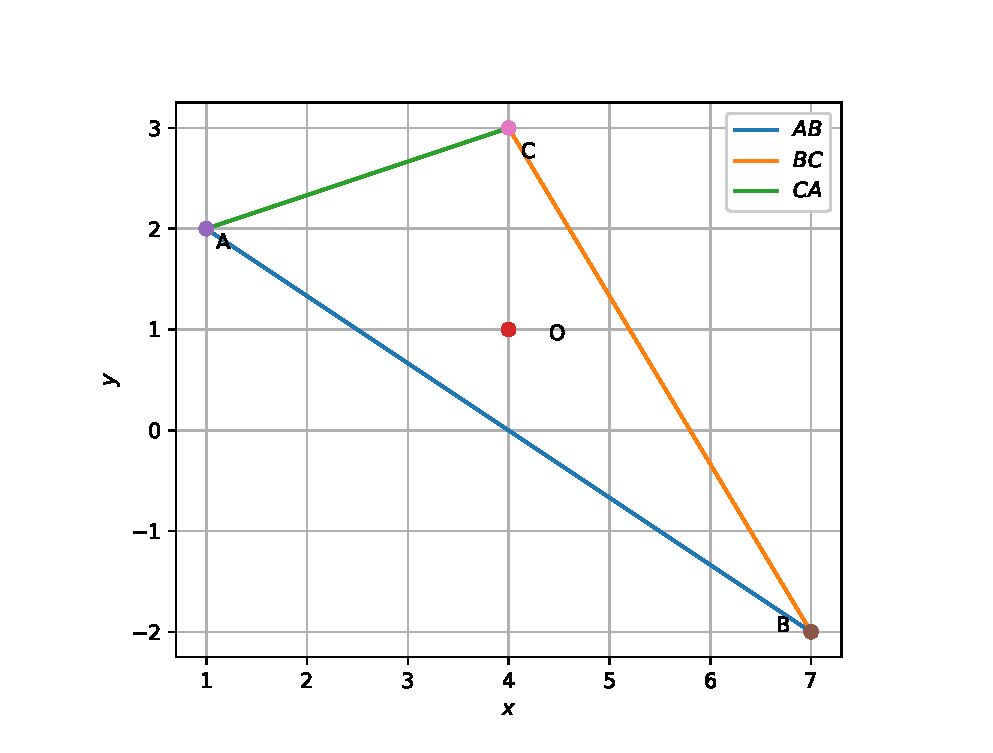
\includegraphics[width=\columnwidth]{./line/figs/triangle.eps}
\caption{}
\label{fig:triangle}
\end{figure}
\end{enumerate}

 
\subsection{Programming}
\renewcommand{\theequation}{\theenumi}

\begin{enumerate}[label=\arabic*.,ref=\thesubsection.\theenumi]
\numberwithin{equation}{enumi}
\item
Find the {\em orthocentre} of  $\triangle ABC$.
\\
\solution The following code finds the required point using \eqref{eq:alt_ap} and \eqref{eq:alt_bq}
.
\begin{lstlisting}
codes/2d/orthocentre.py
\end{lstlisting}

\item Find $\vec{P}$, the foot of the altitude from $\vec{A}$ upon BC.
%
\\
\solution 
\begin{lstlisting}
codes/2d/alt_foot.py
\end{lstlisting}
\item Find $\vec{Q}$ and $\vec{R}$.
\item Draw $AP, BQ$ and $CR$ and verify that they meet at a point 
$\vec{H}$.  
\\
\solution The following code plots the altitudes in Fig. \ref{fig:alt_triangle}
\begin{lstlisting}
codes/2d/alt_draw.py
\end{lstlisting}
\begin{figure}
\centering
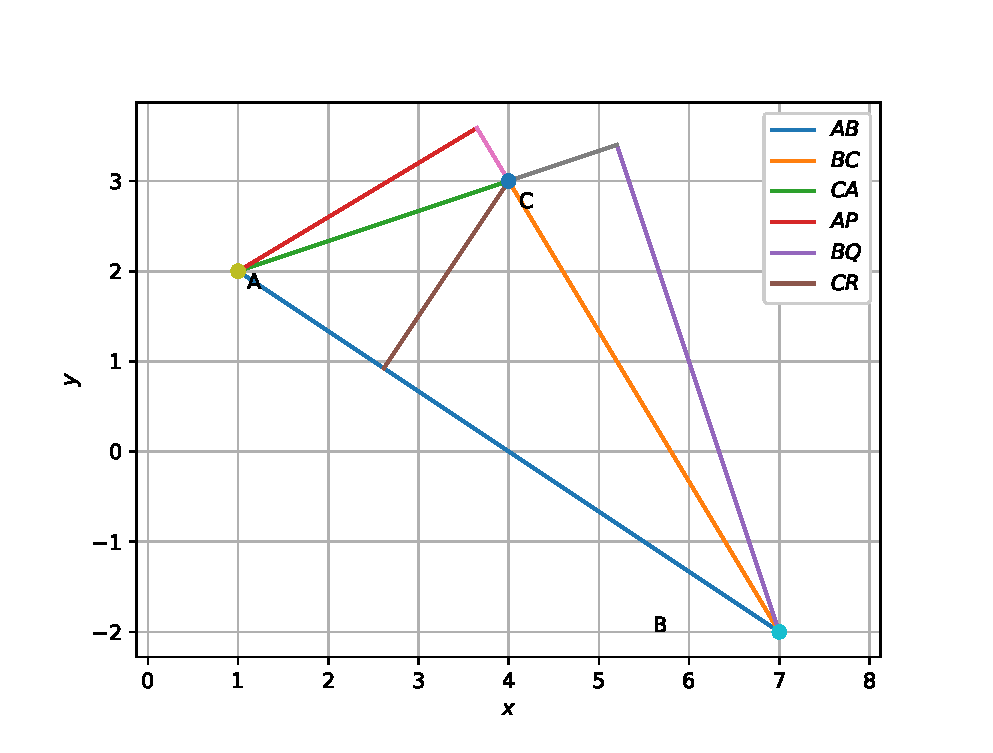
\includegraphics[width=\columnwidth]{./line/figs/alt_triangle.eps}
\caption{}
\label{fig:alt_triangle}
\end{figure}
\item
Find the coordinates of $\vec{D}, \vec{E}$ and $\vec{F}$ of the mid points of $AB, BC$ and $CA$ respectively 
for  $\Delta ABC$. 
\item
Find the equations of $AD,BE$ and $CF$. 
%
\item
\label{prob:median}
Find the point of intersection of $AD$ and $CF$.
\item
Verify that $\vec{O}$ is the point of intersection of $BE,CF$ as 
well.
%as
\item
Graphically show that the medians of $\Delta ABC$ meet at the centroid.
\end{enumerate}

 
\subsection{Solved Problems}
%\documentclass[journal,12pt,twocolumn]{IEEEtran}
%\usepackage{setspace}
%\usepackage{gensymb}
%\usepackage{caption}
%%\usepackage{multirow}
%%\usepackage{multicolumn}
%%\usepackage{subcaption}
%%\doublespacing
%\singlespacing
%\usepackage{csvsimple}
%\usepackage{amsmath}
%\usepackage{multicol}
%%\usepackage{enumerate}
%\usepackage{amssymb}
%%\usepackage{graphicx}
%\usepackage{newfloat}
%%\usepackage{syntax}
%\usepackage{listings}
%\usepackage{iithtlc}
%\usepackage{color}
%\usepackage{tikz}
%\usetikzlibrary{shapes,arrows}
%
%
%
%%\usepackage{graphicx}
%%\usepackage{amssymb}
%%\usepackage{relsize}
%%\usepackage[cmex10]{amsmath}
%%\usepackage{mathtools}
%%\usepackage{amsthm}
%%\interdisplaylinepenalty=2500
%%\savesymbol{iint}
%%\usepackage{txfonts}
%%\restoresymbol{TXF}{iint}
%%\usepackage{wasysym}
%\usepackage{amsthm}
%\usepackage{mathrsfs}
%\usepackage{txfonts}
%\usepackage{stfloats}
%\usepackage{cite}
%\usepackage{cases}
%\usepackage{mathtools}
%\usepackage{caption}
%\usepackage{enumerate}	
%\usepackage{enumitem}
%\usepackage{amsmath}
%%\usepackage{xtab}
%\usepackage{longtable}
%\usepackage{multirow}
%%\usepackage{algorithm}
%%\usepackage{algpseudocode}
%\usepackage{enumitem}
%\usepackage{mathtools}
%\usepackage{hyperref}
%%\usepackage[framemethod=tikz]{mdframed}
%\usepackage{listings}
%    %\usepackage[latin1]{inputenc}                                 %%
%    \usepackage{color}                                            %%
%    \usepackage{array}                                            %%
%    \usepackage{longtable}                                        %%
%    \usepackage{calc}                                             %%
%    \usepackage{multirow}                                         %%
%    \usepackage{hhline}                                           %%
%    \usepackage{ifthen}                                           %%
%  %optionally (for landscape tables embedded in another document): %%
%    \usepackage{lscape}     
%
%
%\usepackage{url}
%\def\UrlBreaks{\do\/\do-}
%
%
%%\usepackage{stmaryrd}
%
%
%%\usepackage{wasysym}
%%\newcounter{MYtempeqncnt}
%\DeclareMathOperator*{\Res}{Res}
%%\renewcommand{\baselinestretch}{2}
%\renewcommand\thesection{\arabic{section}}
%\renewcommand\thesubsection{\thesection.\arabic{subsection}}
%\renewcommand\thesubsubsection{\thesubsection.\arabic{subsubsection}}
%
%\renewcommand\thesectiondis{\arabic{section}}
%\renewcommand\thesubsectiondis{\thesectiondis.\arabic{subsection}}
%\renewcommand\thesubsubsectiondis{\thesubsectiondis.\arabic{subsubsection}}
%
%% correct bad hyphenation here
%\hyphenation{op-tical net-works semi-conduc-tor}
%
%%\lstset{
%%language=C,
%%frame=single, 
%%breaklines=true
%%}
%
%%\lstset{
%	%%basicstyle=\small\ttfamily\bfseries,
%	%%numberstyle=\small\ttfamily,
%	%language=Octave,
%	%backgroundcolor=\color{white},
%	%%frame=single,
%	%%keywordstyle=\bfseries,
%	%%breaklines=true,
%	%%showstringspaces=false,
%	%%xleftmargin=-10mm,
%	%%aboveskip=-1mm,
%	%%belowskip=0mm
%%}
%
%%\surroundwithmdframed[width=\columnwidth]{lstlisting}
%\def\inputGnumericTable{}                                 %%
%\lstset{
%%language=C,
%frame=single, 
%breaklines=true,
%columns=fullflexible
%}
% 
%
%\begin{document}
%%
%\tikzstyle{block} = [rectangle, draw,
%    text width=3em, text centered, minimum height=3em]
%\tikzstyle{sum} = [draw, circle, node distance=3cm]
%\tikzstyle{input} = [coordinate]
%\tikzstyle{output} = [coordinate]
%\tikzstyle{pinstyle} = [pin edge={to-,thin,black}]
%
%\theoremstyle{definition}
%\newtheorem{theorem}{Theorem}[section]
%\newtheorem{problem}{Problem}
%\newtheorem{proposition}{Proposition}[section]
%\newtheorem{lemma}{Lemma}[section]
%\newtheorem{corollary}[theorem]{Corollary}
%\newtheorem{example}{Example}[section]
%\newtheorem{definition}{Definition}[section]
%%\newtheorem{algorithm}{Algorithm}[section]
%%\newtheorem{cor}{Corollary}
%\newcommand{\BEQA}{\begin{eqnarray}}
%\newcommand{\EEQA}{\end{eqnarray}}
%\newcommand{\define}{\stackrel{\triangle}{=}}
%
%\bibliographystyle{IEEEtran}
%%\bibliographystyle{ieeetr}
%
%\providecommand{\nCr}[2]{\,^{#1}C_{#2}} % nCr
%\providecommand{\nPr}[2]{\,^{#1}P_{#2}} % nPr
%\providecommand{\mbf}{\mathbf}
%\providecommand{\pr}[1]{\ensuremath{\Pr\left(#1\right)}}
%\providecommand{\qfunc}[1]{\ensuremath{Q\left(#1\right)}}
%\providecommand{\sbrak}[1]{\ensuremath{{}\left[#1\right]}}
%\providecommand{\lsbrak}[1]{\ensuremath{{}\left[#1\right.}}
%\providecommand{\rsbrak}[1]{\ensuremath{{}\left.#1\right]}}
%\providecommand{\brak}[1]{\ensuremath{\left(#1\right)}}
%\providecommand{\lbrak}[1]{\ensuremath{\left(#1\right.}}
%\providecommand{\rbrak}[1]{\ensuremath{\left.#1\right)}}
%\providecommand{\cbrak}[1]{\ensuremath{\left\{#1\right\}}}
%\providecommand{\lcbrak}[1]{\ensuremath{\left\{#1\right.}}
%\providecommand{\rcbrak}[1]{\ensuremath{\left.#1\right\}}}
%\theoremstyle{remark}
%\newtheorem{rem}{Remark}
%\newcommand{\sgn}{\mathop{\mathrm{sgn}}}
%\providecommand{\abs}[1]{\left\vert#1\right\vert}
%\providecommand{\res}[1]{\Res\displaylimits_{#1}} 
%\providecommand{\norm}[1]{\lVert#1\rVert}
%\providecommand{\mtx}[1]{\mathbf{#1}}
%\providecommand{\mean}[1]{E\left[ #1 \right]}
%\providecommand{\fourier}{\overset{\mathcal{F}}{ \rightleftharpoons}}
%%\providecommand{\hilbert}{\overset{\mathcal{H}}{ \rightleftharpoons}}
%\providecommand{\system}{\overset{\mathcal{H}}{ \longleftrightarrow}}
%	%\newcommand{\solution}[2]{\textbf{Solution:}{#1}}
%\newcommand{\solution}{\noindent \textbf{Solution: }}
%\newcommand{\myvec}[1]{\ensuremath{\begin{pmatrix}#1\end{pmatrix}}}
%\providecommand{\dec}[2]{\ensuremath{\overset{#1}{\underset{#2}{\gtrless}}}}
%\DeclarePairedDelimiter{\ceil}{\lceil}{\rceil}
%%\numberwithin{equation}{section}
%%\numberwithin{problem}{subsection}
%%\numberwithin{definition}{subsection}
%\makeatletter
%\@addtoreset{figure}{section}
%\makeatother
%
%\let\StandardTheFigure\thefigure
%%\renewcommand{\thefigure}{\theproblem.\arabic{figure}}
%\renewcommand{\thefigure}{\thesection}
%
%
%%\numberwithin{figure}{subsection}
%
%%\numberwithin{equation}{subsection}
%%\numberwithin{equation}{section}
%%\numberwithin{equation}{problem}
%%\numberwithin{problem}{subsection}
%\numberwithin{problem}{section}
%%%\numberwithin{definition}{subsection}
%%\makeatletter
%%\@addtoreset{figure}{problem}
%%\makeatother
%\makeatletter
%\@addtoreset{table}{section}
%\makeatother
%
%\let\StandardTheFigure\thefigure
%\let\StandardTheTable\thetable
%\let\vec\mathbf
%%%\renewcommand{\thefigure}{\theproblem.\arabic{figure}}
%%\renewcommand{\thefigure}{\theproblem}
%
%%%\numberwithin{figure}{section}
%
%%%\numberwithin{figure}{subsection}
%
%
%
%\def\putbox#1#2#3{\makebox[0in][l]{\makebox[#1][l]{}\raisebox{\baselineskip}[0in][0in]{\raisebox{#2}[0in][0in]{#3}}}}
%     \def\rightbox#1{\makebox[0in][r]{#1}}
%     \def\centbox#1{\makebox[0in]{#1}}
%     \def\topbox#1{\raisebox{-\baselineskip}[0in][0in]{#1}}
%     \def\midbox#1{\raisebox{-0.5\baselineskip}[0in][0in]{#1}}
%
%\vspace{3cm}
%
%\title{ 
%	\logo{
%The Straight Line and Linearity
%	}
%}
%
%\author{ G V V Sharma$^{*}$% <-this % stops a space
%	\thanks{*The author is with the Department
%		of Electrical Engineering, Indian Institute of Technology, Hyderabad
%		502285 India e-mail:  gadepall@iith.ac.in. All content in this manual is released under GNU GPL.  Free and open source.}
%	
%}	
%
%\maketitle
%
%%\tableofcontents
%
%\bigskip
%
%\renewcommand{\thefigure}{\theenumi}
%\renewcommand{\thetable}{\theenumi}
%
%
%\begin{abstract}
%	Solved problems from JEE mains papers related to 2D lines in coordinate geometry are 
%available in this document.  These problems are solved using linear algebra/matrix analysis.
%\end{abstract}
%\begin{enumerate}[label=\arabic*]
%\numberwithin{equation}{enumi}

\renewcommand{\theequation}{\theenumi}

\begin{enumerate}[label=\arabic*.,ref=\thesubsection.\theenumi]
\item A straight line through the origin   $\vec{O}$ meets the lines
\begin{align} 
\label{eq:line_1}
\myvec{4 & 3}\vec{x} &= 10
\\
\myvec{8 & 6}\vec{x} +5&= 0
\end{align} 
%
at $\vec{A}$ and $\vec{B}$ respectively.  Find the ratio in which  $\vec{O}$ divides $AB$.
\\
\solution Let 
\begin{align} 
\vec{n} =\myvec{4 \\ 3}
\end{align} 
%
Then \eqref{eq:line_1} can be expressed as
\begin{align} 
\label{eq:line_1_normal}
\vec{n}^T\vec{x} &= 10
\\
2\vec{n}^T\vec{x} &= -5
\end{align} 
%
and since $\vec{A}, \vec{B}$ satisfy \eqref{eq:line_1_normal} respectively,
\begin{align} 
\label{eq:line_1_normal_a}
\vec{n}^T\vec{A} &= 10
\\
2\vec{n}^T\vec{B} &= -5
\label{eq:line_1_normal_b}
\end{align} 
%
Let  $\vec{O}$ divide the segment $AB$ in the ratio $k:1$. Then
\begin{align} 
\label{eq:line_1_section}
\vec{O}=\frac{k\vec{B} +\vec{A} }{k+1}
\end{align} 
%
\begin{align} 
%\label{eq:line_1_section}
\because \vec{O}&= \vec{0},
\\
\vec{A} &=-k\vec{B}
\end{align} 
%
Substituting in \eqref{eq:line_1_normal_a}, and simplifying, 
\begin{align} 
\label{eq:line_1_normal_subs_a}
\vec{n}^T\vec{B} &= \frac{10}{-k}
\\
\vec{n}^T\vec{B} &= \frac{-5}{2}
%\label{eq:line_1_normal_b}
\end{align} 
resulting in 
\begin{align} 
\frac{10}{-k} = \frac{-5}{2} \implies k = 4
\end{align} 
\item The 
point 
\begin{equation} 
\vec{P}=\myvec{2\\ 1} 
\end{equation} 
is translated parallel to the line 
\begin{equation} 
\label{line_2}
L: \myvec{1 & -1}\vec{x} = 4 
\end{equation} 
% 
by $d =2\sqrt{3}$ units.  If the new point $\vec{Q}$ lies in the third 
quadrant, then find the equation of the line passing through $\vec{Q}$ and perpendicular to $L$. 
\\
\solution From \eqref{line_2}, the direction vector of $L$ is
\begin{equation} 
\label{line_2_m}
\vec{m} = \myvec{1 \\ 1} 
\end{equation} 
Thus, 
\begin{equation} 
\label{line_2_q}
\vec{Q}= \vec{P} + \lambda \vec{m}
\end{equation} 
However, 
\begin{align} 
PQ &= d
\\
\implies\norm{\vec{P}- \vec{Q}} &= \abs{\lambda}\norm{\vec{m}} =  d
\\
\implies \lambda &= \pm \frac{d}{\norm{\vec{m}}} = \pm \sqrt{6}
\label{line_2_lam}
\end{align} 
%
\begin{align} 
\because \norm{\vec{m}} = \sqrt{\vec{m}^T\vec{m}}= \sqrt{2}
\end{align} 
%
from \eqref{line_2_m}.  Since $\vec{Q}$ lies in the third quadrant, from \eqref{line_2_q} and \eqref{line_2_lam},
\begin{align} 
\vec{Q} = \myvec{2\\ 1}  -  \sqrt{6}\myvec{1\\ 1} =  \myvec{2-\sqrt{6}\\ 1-\sqrt{6}}
\end{align} 
%
The equation of the desired line is then obtained as 
\begin{align} 
\label{line_2_final}
\vec{m}^T\brak{\vec{x}-\vec{Q}}&= 0
\\
 \myvec{1 & 1}\vec{x} &= 3 -2\sqrt{6}
\end{align} 
\item Two sides of a rhombus are along the lines
\begin{align}
\label{eq:lines_4_ab}
AB: \myvec{1 & -1}\vec{x} + 1 &=0
\\
AD: \myvec{7 & -1}\vec{x} -5 &=0.
\label{eq:lines_4_ad}
\end{align}
%
If its diagonals intersect at 
\begin{equation}
\vec{P}=\myvec{-1\\ -2},
\label{eq:lines_4_p}
\end{equation}
find its vertices.
\\
\solution From \eqref{eq:lines_4_ab} and \eqref{eq:lines_4_ad},
\begin{align}
\myvec{1 & -1 \\ 7 & -1}\vec{A}  &=\myvec{-1 \\ 5}
\end{align}
%
By row reducing the augmented matrix
\begin{align}
\myvec{1 & -1 & -1\\ 7 & -1 & 5}  &\leftrightarrow \myvec{1 & -1 & -1\\ 0 & 6 & 12}\leftrightarrow \myvec{1 & -1 & -1\\ 0 & 1 & 2}
\nonumber \\
&\leftrightarrow \myvec{1 & 0 & 1\\ 0 & 1 & 2} \implies \vec{A}=\myvec{1\\ 2},
\label{eq:lines_4_a}
\end{align}
%
Since diagonals of a rhombus bisect each other, 
\begin{align}
\vec{P}&=\frac{\vec{A}+\vec{C}}{2}
\nonumber \\
\vec{C}&=2\vec{P}-\vec{A} = \myvec{-3\\-6}
\label{eq:lines_4_c}
\end{align}
%
\begin{align}
\because AD \parallel BC,&
\nonumber \\
BC: \myvec{7 & -1}\brak{\vec{x}-\vec{C}} &=0
\nonumber \\
\implies \myvec{7 & -1}\vec{x} &=-15
\label{eq:lines_4_bc}
\end{align}
%
From \eqref{eq:lines_4_ab} and \eqref{eq:lines_4_bc},
\begin{align}
 \myvec{7 & -1 \\ 1 & -1}\vec{B} &=\myvec{-15 \\ -1}
\end{align}
resulting in the augmented matrix
\begin{align}
& \myvec{7 & -1 & -15\\ 1 & -1 & -1} 
\leftrightarrow
 \myvec{7 & -1 & -15\\ 0 & 3 & -4} 
\nonumber \\
&\leftrightarrow
 \myvec{3 & 0 & -7\\ 0 & 3 & -4} \implies \vec{B} = -\frac{1}{3}\myvec{7\\4}
\end{align}
\begin{align}
\because AB \parallel CD,&
\nonumber \\
CD: \myvec{1 & -1}\brak{\vec{x}-\vec{C}} &=0
\nonumber \\
\implies \myvec{1 & -1}\vec{x} &=3
\label{eq:lines_4_cd}
\end{align}
%
From \eqref{eq:lines_4_ad} and \eqref{eq:lines_4_cd},
\begin{align}
 \myvec{7 & -1 \\ 1 & -1}\vec{D} &=\myvec{5 \\ 3}
\end{align}
resulting in the augmented matrix
\begin{align}
& \myvec{7 & -1 & 5\\ 1 & -1 & 3} 
\leftrightarrow
 \myvec{7 & -1 & 5\\ 0 & 3 & -8} 
\nonumber \\
&\leftrightarrow
 \myvec{3 & 0 & 1\\ 0 & 3 & -8} \implies \vec{D} = \frac{1}{3}\myvec{1\\-8}
\end{align}

%From \eqref{eq:lines_4_p} and \eqref{eq:lines_4_a}
%\begin{align}
%AP =\norm{\vec{A}-\vec{P}} = 2\sqrt{5} =d (say)
%\end{align}
%%
%The direction vector of $AP$ is 
%\begin{align}
%\vec{m} &=\vec{A}-\vec{P} = 2\myvec{1\\ 2}
%\\
%\implies \norm{\vec{m}} &= 2\sqrt{5}
%\end{align}
%Since the direction of $AP$ is the same as $AC$,
%\begin{align}
%\vec{C} &=\vec{P}-d\frac{\vec{m}}{\norm{\vec{m}}} 
%\nonumber \\
%&= -\myvec{1\\ 2}- 2\myvec{1\\ 2} = \myvec{-3\\ -6}
%\end{align}
%
%Let $\vec{n}\perp\vec{m}$. Then 
%\begin{align}
%\vec{n} &=\myvec{2\\ -1}
%\end{align}
%%
%and 
%\begin{align}
%\vec{B,D} &=\vec{P}\pm d\frac{\vec{n}}{\norm{\vec{n}}} 
%\nonumber \\
%&=-\myvec{1\\ 2}\pm 2\myvec{2\\ -1} = \myvec{5\\ 0}, \myvec{-3\\ 4}
%\end{align}

\item Let $k$ be an integer such that the triangle with vertices
\begin{equation}
\label{eq:lines_5}
\vec{A} = \myvec{k\\-3k},
\vec{B} =\myvec{5\\k},
\vec{C} =\myvec{-k\\2}
\end{equation}
has area 28.  Find the orthocentre of this triangle.
%
\\
\solution Let $\vec{m}_1$ be the direction vector of $BC$.  Then,
\begin{align}
\label{eq:lines_5_m1}
\vec{m}_1 = \myvec{5+k\\k-2},
\end{align}
%
If $AD$ be an altitude, its equation can be obtained as
\begin{align}
\label{eq:lines_5_m1a}
\vec{m}_1^{T}\brak{\vec{x}-\vec{A}} = 0
\end{align}
%
Similarly, considering the side $AC$  the equation of the altitude $BE$ is
\begin{align}
\label{eq:lines_5_m2b}
\vec{m}_2^{T}\brak{\vec{x}-\vec{B}} = 0
\end{align}
%
where 
\begin{align}
\label{eq:lines_5_m2}
\vec{m}_2 = \myvec{2k\\-2-3k},
\end{align}
The orthocentre is obtained by solving \eqref{eq:lines_5_m1a}
and \eqref{eq:lines_5_m2b} using the matrix equation
\begin{align}
\myvec{\vec{m}_1\\ \vec{m}_2}^T \vec{x} 
= \myvec{ \vec{m}_1^T\vec{A}\\ \vec{m}_2^T
\vec{B}}
\end{align}
%
which can be expressed using \eqref{eq:lines_5_m1}, 
\eqref{eq:lines_5_m2}, 
\eqref{eq:lines_5_m1a} and 
\eqref{eq:lines_5_m2b}
as 
\begin{align}
\myvec{5+k & k-2 \\2k & -2-3k} \vec{x} 
&= \myvec{ k^2+5k+6k-3k^2\\ 10k-2k-3k^2}
\nonumber \\
&= k\myvec{ 11-4k\\ 8-3k}
\label{eq:lines_5_h}
\end{align}
%
%The solution to the above is 
%\begin{align}
%\vec{x} &= k\myvec{5+k & k-2 \\2k & -2-3k}^{-1} \myvec{ 11-4k\\ 8-3k}
%\nonumber \\
%&= \frac{k}{-3k^2-17k-10-2k^2+4k}
%\nonumber \\
%&\times \myvec{-2-3k & -k+2 \\-2k & 5+k} \myvec{ 11-4k\\ 8-3k}
%\nonumber \\
%&= \frac{k}{5k^2+13k+10}
%\nonumber \\
%&\times \myvec{2+3k & k-2 \\2k & -5-k} \myvec{ 11-4k\\ 8-3k}
%\nonumber \\
%&= \frac{k}{5k^2+13k+10}
%\nonumber \\
%&\times 
%\myvec{ 22-12k^2-8k+33k -3k^2+6k+8k-16 \\ 22k-8k^2-40+15k-8k+3k^2}
%\nonumber \\
%&= \frac{k}{5k^2+13k+10}
%\myvec{ 6+39k-15k^2 \\ -40+29k-5k^2}
%\end{align}
From \eqref{eq:lines_5}, using the expression for the area of triangle,
\begin{align}
\begin{vmatrix}
k & 5 & -k\\-3k & k & 2 \\ 1 & 1 & 1
\end{vmatrix} = 56
\nonumber \\
\implies
\begin{vmatrix}
k & 5-k & -2k\\-3k & 4k & 2+3k \\ 1 & 0 & 0
\end{vmatrix} = 56
\end{align}
%
resulting in
\begin{align}
\brak{5-k}
\brak{2+3k}+8k^2=56
\\
\implies 5k^2+13k-46 = 0
\\
\text{or, } k = 2, -\frac{23}{5}
\end{align}
Substituting the above in \eqref{eq:lines_5_h} and solving yields the orthocentre.
\item If an equilateral triangle, having centroid at the origin, has a side along the line
\begin{equation}
\label{eq:lines_6_ab}
\myvec{1 & 1}\vec{x} = 2,
\end{equation}
then find the area of this triangle. Also draw the equilateral triangle and two medians to verify your results.
\\
\solution Let the vertices be $\vec{A},\vec{B},\vec{C}$. From the given information, 
\begin{align}
\frac{\vec{A}+\vec{B}+\vec{C}}{3} &= \vec{0}
\nonumber \\
\implies 
\vec{A}+\vec{B}+\vec{C} = \vec{0}
\label{eq:lines_6_abc}
\end{align}
%
If $AB$ be the line in \eqref{eq:lines_6_ab},
%\begin{equation}
%\label{eq:lines_6_nab}
%\myvec{1 & 1}\brak{\vec{A}-\vec{B}} = 0
%\end{equation}
%%
%Thus, the direction vector of $AB$ is 
%\begin{align}
%\label{eq:lines_6_mab}
%\vec{m} = \myvec{1 \\ -1}
%\end{align}
the equation of 
$CF$, where 
\begin{align}
\vec{F} = \frac{\vec{A}+\vec{B}}{2} 
\end{align}
is 
%
\begin{align}
\label{eq:lines_6_cf}
\myvec{1 & -1}\vec{x} = 0
\end{align}
since $CF$ passes through the origin and $CF\perp AB$. From \eqref{eq:lines_6_ab}
and \eqref{eq:lines_6_cf},
\begin{align}
\label{eq:lines_6_fmat}
\myvec{1 & 1 \\1 & -1}\vec{F} = \myvec{2 \\ 0}
\end{align}
%
Forming the augmented matrix, 
\begin{align}
\myvec{1 & 1 &2 \\1 & -1 & 0} &\leftrightarrow \myvec{1 & 1 &2 \\0 & 2 & 2} \leftrightarrow \myvec{1 & 1 &2 \\0 & 1 & 1} 
\nonumber \\
&\leftrightarrow \myvec{1 & 0 &1 \\0 & 1 & 1} \implies \vec{F} = \myvec{1 \\ 1}
\label{eq:lines_6_f}
\end{align}
From \eqref{eq:lines_6_abc},
\begin{align}
\vec{C}=-\brak{\vec{A}+\vec{B}}=-2\vec{F} = -2\myvec{1 \\ 1}
\label{eq:lines_6_c}
\end{align}
after substituting from \eqref{eq:lines_6_f}.  Thus, 
\begin{align}
CF &= \norm{\vec{C}-\vec{F}} = 3\sqrt{2} 
\\
\implies AB &=  CF\frac{2}{\sqrt{3}} = 2\sqrt{6}
\label{eq:lines_6_cflen}
\end{align}
and the area of the triangle is 
\begin{align}
\frac{1}{2} AB \times CF = 6\sqrt{3}
\end{align}


\item A square, of each side 2, lies above the $x$-axis and has one vertex at the origin.  If one of the sides 
passing through the origin makes an angle $30^{\degree}$ with the positive direction of the $x$-axis, then 
find the 
sum of the $x$-coordinates of the vertices of the square.
\\
\solution Consider the square $ABCD$ with $\vec{A} = \vec{0}, AB = 2$ such that $\vec{B}$ and $\vec{D}$ lie on the $x$ and $y$-axis respectively. Then 
\begin{align}
\vec{A}+\vec{B}+\vec{C}+\vec{D} = 4\myvec{1 \\ 1}
\label{eq:lines_7_abcdsum}
\end{align}
%
Multiplying \eqref{eq:lines_7_abcdsum} with the rotation matrix 
\begin{align}
\label{eq:lines_7_t}
\vec{T} = \myvec{\cos \theta & -\sin \theta \\ \sin \theta & \cos \theta},
\end{align}
\begin{align}
\vec{T}\brak{\vec{A}+\vec{B}+\vec{C}+\vec{D}} &= 4\myvec{\cos \theta & -\sin \theta \\ \sin \theta & \cos \theta}\myvec{1 \\ 1}
\nonumber \\
&= 4\myvec{\cos \theta  -\sin \theta \\ \cos \theta + \sin \theta}
%\nonumber \\
\end{align}
\begin{multline}
\implies \myvec{1 & 0}\vec{T}\brak{\vec{A}+\vec{B}+\vec{C}+\vec{D}} 
\\
= 4\brak{\cos \theta  -\sin \theta}
= 2\brak{\sqrt{3}-1}
\end{multline}
%
for $\theta = 30^{\degree}$. Draw the square with sides on the axis as well as the rotated square in the same graph to verify your result.


%\item Find the locus of the point of intersection of the lines
%\begin{align}
%\myvec{\sqrt{2} & -1 }\vec{x} + 4 \sqrt{2}k &= 0
%\\
%\myvec{\sqrt{2}k & k }\vec{x} - 4 \sqrt{2} &= 0
%\end{align}

\end{enumerate}
%\section{Trigonometry}
%\begin{enumerate}[label=\thesection.\arabic*
%,ref=\thesection.\theenumi]
%
%\item In $\triangle PQR$, which is not right angled, let
%\begin{align}
%PQ = r, QR = p, RP = q
%\end{align}
%%
%The median $RS$ and the altitude $PE$  intersect at $\vec{O}$. $p =\sqrt{3}, q = 1$ and the radius of the circumcircle  of $\triangle PQR = k = 1$.  
%\item Find  $RS$
%\\
%\solution Using the sine formula,
%\begin{align}
%\frac{p}{\sin P}=\frac{q}{\sin Q} = 2k
%\\
%\implies \sin P = \frac{\sqrt{3}}{2}, \sin Q = \frac{1}{2}
%\end{align}
%If $\angle R \ne \frac{\pi}{2}$, the only possible solution is 
%\begin{align}
%\angle P = \frac{2\pi}{3},
%\angle Q = \frac{\pi}{6},
%\angle R = \frac{\pi}{6}
%\end{align}
%%
%$\because \angle Q = \angle R, q = r = 1$.  The given information is shown in Fig. \ref{fig:2019_8}
%\begin{figure}
%\centering
%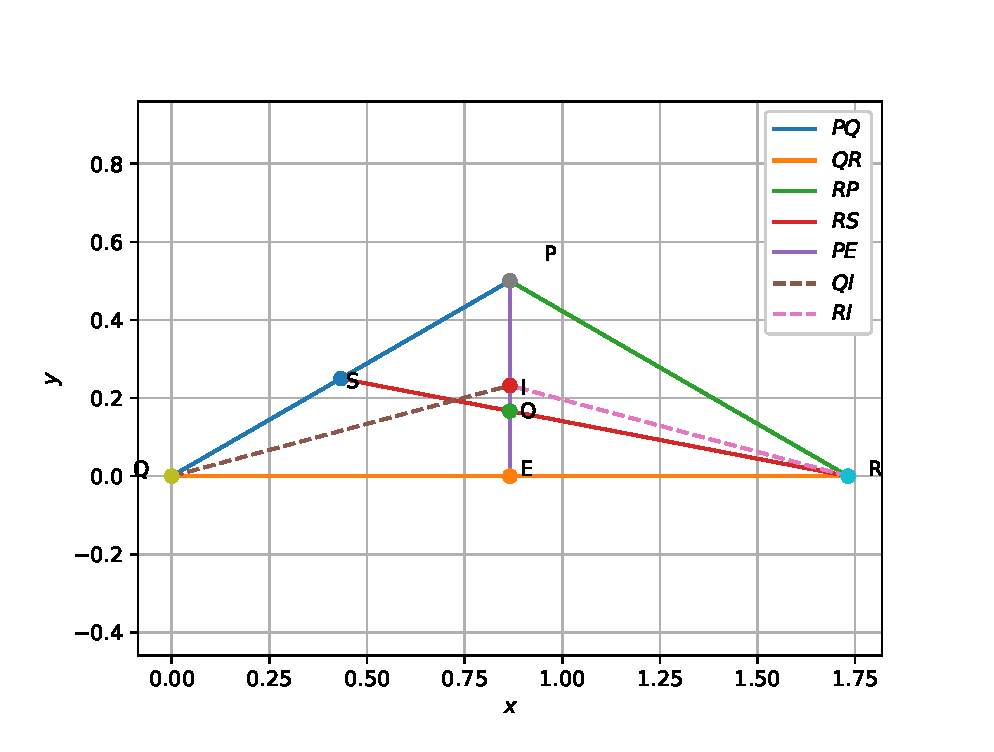
\includegraphics[width=\columnwidth]{./line/figs/2019_8.eps}
%\caption{}
%\label{fig:2019_8}
%\end{figure}
%%
%Using the cosine formula, 
%\begin{align}
%RS &= \sqrt{q^2+\brak{\frac{r}{2}}^2-qr\cos P}
%\\
%&= \sqrt{1+\frac{1}{4}+\frac{1}{2}} = \sqrt{\frac{7}{2}}
%\end{align}
%\item Find $OE$.
%\\
%\solution 
%Using Baudhayana's theorem,
%\begin{align}
%OE  &= \sqrt{OR^2 - ER^2}
%\\
%&= \sqrt{\brak{\frac{2RS}{3}}^2 - \brak{\frac{p}{2}}^2} 
%\\
%&= \sqrt{\frac{7}{9}-\frac{3}{4}} = \frac{1 }{6}
%\end{align}
%%
%\item Find the area of $\triangle SOE$
%\\
%\solution
%$\because$ $PE$ and $RS$ are medians, 
%\begin{align}
%\text{ar}\brak{\triangle SOE }&= \frac{1}{4}\text{ar}\brak{\triangle POR},
%\\
%\text{ar}\brak{\triangle POR }&=  \frac{2}{3}\text{ar}\brak{\triangle PER},
%\\
%\text{ar}\brak{\triangle PER }&=  \frac{1}{2}\text{ar}\brak{\triangle PQR},
%\\
%\implies \text{ar}\brak{\triangle SOE} &= \frac{1}{12}\text{ar}\brak{\triangle PQR}
%&= \frac{\sqrt{3}}{24}
%\end{align}
%
%\item Find the radius of the incircle of $\triangle PQR $.
%%
%\\
%\solution
%I is the incentre in Fig. \ref{fig:2019_8}.  The radius of the incircle is 
%\begin{align}
%\frac{p}{2\cos\frac{Q}{2}} &= \frac{p}{\sqrt{2\brak{1+\cos Q}}}
%\\ &= \sqrt{\frac{3}{1+\sqrt{3}}}
%\end{align}
%%
%\item Repeat all the above exercises using vector algebra and plot Fig. \ref{fig:2019_8}.
%\end{enumerate}
%
%\end{document}
 
\subsection{JEE Exercises}
\renewcommand{\theequation}{\theenumi}
\begin{enumerate}[label=\arabic*.,ref=\thesubsection.\theenumi]
\numberwithin{equation}{enumi}

    \item Find the area enclosed within the curve $\abs{x} + \abs{y} = 1 $.
    \item Find the equation of the line about which y=$10^x$ is the reflection of y=$\log_{10}x$.

    \item If $3a+2b+4c=0$, find the intersection of the  set of lines 
  \begin{align} 
    \myvec{a & b}\vec{x} + c &= 0.
    \end{align}
    \item Given the points $A=\myvec{0 \\ 4}$ and $B=\myvec{0 \\ -4}$, find the equation of the locus of the point $P=\myvec{x \\ y}$ such that $\abs{AP-BP} $=6.
    \item If a,b and c are in A.P, show that  the straight line 
\begin{align} 
    \myvec{a & b}\vec{x} + c &= 0
    \end{align}
will always pass through a fixed point and find its coordinates.
    \item Find the quadrant in which the orthocentre of the triangle formed by the lines 
\begin{align} 
    \myvec{1 & 1}\vec{x}  &= 1
\\
    \myvec{2 & 3}\vec{x}  &= 6
\\
    \myvec{4 & -1}\vec{x} + 4 &= 0
    \end{align} lies.
    \item Let the algebraic sum of the perpendicular distances from the points $\myvec{2 \\ 0}$,  $\myvec{0 \\ 2}$ and $\myvec{1 \\ 1}$ to a variable straight line be zero.  Show that  the line passes through a fixed point and find its  coordinates. 
    \item The vertices of a triangle are $\vec{A}=\myvec{-1 \\ -7},\vec{B}=\myvec{5 \\ 1}$ and $\vec{C}=\myvec{1 \\ 4}$. Find the equation of the bisector of $\angle ABC$.
    \item Verify if the straight line 
\begin{align} 
    \myvec{5 & 4}\vec{x} &= 0
    \end{align} passes through the point of intersection of the straight lines \begin{align} 
    \myvec{1 & 2}\vec{x} - 10 &= 0
    \end{align} and \begin{align} 
    \myvec{2 & 1}\vec{x} + 5 &= 0
    \end{align}
    \item Do the lines \begin{align} 
    \myvec{2 & 3}\vec{x} + 19 &= 0
    \end{align} and \begin{align} 
    \myvec{9 & 6}\vec{x} - 17 &= 0
    \end{align} cut the coordinate axes in concyclic points?
    \item The points $\myvec{-a\\b}$,\myvec{0\\0},\myvec{a\\b} and \myvec{a^2\\ab} are:
    \begin{enumerate}
    \item  Collinear
    \item  Vertices of a parallelogram
    \item  Vertices of a rectangle
    \item  None of these
    \end{enumerate}
    \item The point $\myvec{4 \\ 1}$ undergoes the following three transformations successively
    (i) Reflection about the line \begin{align} 
    \myvec{-1 & 1}\vec{x} &= 0
    \end{align}
    (ii)Translation through a distance 2 units along the positive direction of x-axis
    (iii) Rotation through an angle $\frac{\pi}{4}$ about the origin in counter clockwise direction.
    Find  the final position of the point.
\item The straight lines \begin{align} 
    \myvec{1 & 1}\vec{x} &= 0
\\
    \myvec{3 & 1}\vec{x} - 4 &= 0
\\
    \myvec{1 & 3}\vec{x} - 4 &= 0
    \end{align}form a triangle which is
    \begin{enumerate}
     \item isosceles
     \item equilateral
     \item right angled
     \item none of these
     \end{enumerate}
    \item If $\vec{P}=\myvec{1\\0}$, $\vec{Q}=\myvec{-1\\0}$ and $\vec{R}=\myvec{2\\0}$ are three given points, then the locus of the point $\vec{S}$ satisfying the relation $SQ^2+SR^2=2SP^2$, is
    \begin{enumerate}
     \item  a straight line parallel to X-axis
     \item a circle passing through the origin
     \item a circle with centre at the origin
     \item  a straight line parallel to Y-axis.
     \end{enumerate}
    \item Line L has intercepts a and b on the coordinate axes.When the axes are rotated through a given angle, keeping the origin fixed, the same line L has intercepts p and q, then
    \begin{enumerate}
     \item  $a^2+b^2=p^2+q^2$
     \item  $\frac{1}{a^2}+\frac{1}{b^2}=\frac{1}{p^2}+\frac{1}{q^2}$
     \item  $a^2+p^2=b^2+q^2$
     \item  $\frac{1}{a^2}+\frac{1}{p^2}=\frac{1}{b^2}+\frac{1}{q^2}$
     \end{enumerate}
    \item If the sum of the distances of a point from two perpendicular lines in a plane is 1, then its locus is
    \begin{enumerate}
     \item  Square
     \item  Circle
     \item  Straight line
     \item  Two intersecting lines
     \end{enumerate}
    \item The locus of a variable point whose distances from $\myvec{-2\\0}$ is $\frac{2}{3}$ times its distance from the line $x=-\frac{9}{2}$ is
    \begin{enumerate}
     \item  Ellipse
     \item  Parabola
     \item  Hyperbola
     \item  None of these
    \end{enumerate}
    \item The equations of a pair of opposite sides of a parallelogram are  
\begin{align} 
x^2-5x+6 = 0
\\
y^2-6y+5 = 0
\end{align}
Find  the equations of its diagonals. 
    \item Find the orthocentre of the triangle formed by the lines 
\begin{align}
    \vec {x}^T\myvec{0 & 1 \\ 1 & 0} \vec{x} &=0
    \end{align} 
and 
\begin{align}
\myvec{1 & 1} \vec x =1
    \end{align} 
    \item Let PQR be an isosceles triangle, right angled at  $\vec{P}=\myvec{2\\1}$. If the equation of the line QR is \begin{align}\myvec{2 & 1}\vec{x} = 3, \end{align} then find the equation representing the pair of lines PQ and PR is
    \item If $x_1,x_2,x_3$ as well as $y_1,y_2,y_3$ are in G.P with the same common ratio, then the points\myvec{x_1\\y_1},\myvec{x_2\\y_2} and \myvec{x_3\\y_3}
    \begin{enumerate}
     \item  lie on a straight line
     \item  lie on a ellipse
    \item  lie on a circle
    \item  are the vertices of a triangle
    \end{enumerate}
    \item Let PS be the median of the triangle with vertices $\vec{P}=\myvec{2\\2}, \vec{Q}=\myvec{6\\-1}$ and $\vec{R}=\myvec{7\\3}$. Find the equation of the line passing through $\myvec{1\\-1}$ and parallel to PS.
    \item Find the incentre of the triangle with vertices $\myvec{1\\\sqrt{3}},\myvec{0\\0}$ and $\myvec{2\\0}$. 
    \item The number of integer values of $m$, for which the x coordinate of the point of intersection of the lines \myvec{3\\4}$\vec {x}=9$ and \myvec{-m\\1}$\vec {x} -1=0$  is also an integer, is
    \begin{enumerate}
     \item  2
     \item  0
     \item  4
     \item  1
     \end{enumerate}
    \item Find the area of the parallelogram formed by the lines \myvec{-m\\1}$\vec {x}$=0, \myvec{-m\\1}$\vec {x}$+1=0 ,\myvec{-n\\1}$\vec {x}$=0 and \myvec{-n\\1}$\vec {x}$+ 1 =0.
    \item Let $0 <\alpha< \frac{\pi}{2}$  be a fixed angle. If
    $\vec{P}=\myvec{\cos\theta \\ \sin \theta}$ and $\vec{Q}=\myvec{\cos\brak{\alpha-\theta}\\ \sin\brak{\alpha-\theta}}$
    then the $\vec{Q}$ is obtained from $\vec{ P}$ by
    \begin{enumerate}
     \item  clockwise rotation around origin through an angle$\alpha$
     \item  anticlockwise rotation around origin through an angle$\alpha$
     \item  reflection in the line through origin with slope $\tan \alpha$
     \item  reflection in the line through origin with slope $\tan \frac{\alpha}{2}$
     \end{enumerate}
    \item Let $\vec{P}=\myvec{-1\\0} \vec{Q}=\myvec{0\\0}$ and $\vec{R}=\myvec{3\\3\sqrt{3}}$ be three points. Then find the equation of the bisector of the angle PQR.
    \item A straight line through the origin $\vec{O}$ meets the parallel lines \begin{align} \myvec{4 & 2} \vec {x} &= 9\end{align} and \begin{align} \myvec{2 & 1} \vec {x} + 6 &= 0\end{align} at points $\vec{P}$ and $\vec{Q}$ respectively. Find the ratio in which $\vec{O}$ divides the segment PQ. 
    \item The number of integral points (integral points means both the coordinate should be integer) exactly in the interior of the triangle with the vertices \myvec{0\\0} , \myvec{0\\21} and  \myvec{21\\0} is 
    \begin{enumerate}
     \item 133
     \item 190
     \item 233
     \item 105
     \end{enumerate}
    \item Find the orthocentre of a triangle with vertices   \myvec{0\\0},\myvec{3\\4},\myvec{4\\0} 
    \item Find the area of the triangle formed by the line \begin{align} \myvec{1 & 1} \vec {x} &= 3\end{align} and angle bisectors of the pair of straight lines \begin{align}\vec{x}^T \myvec{1 & 0 \\ 0 & -1} \vec {x} + \myvec{0 & 2} \vec {x} &= 1.\end{align}
    \item Let $\vec{O}= \myvec{0\\0}, \vec{P}=\myvec{3\\4}, \vec{Q}= \myvec{6\\0}$  be the vertices of the triangle OPQ. The point $\vec{R}$ inside the triangle OPQ is such that the triangles OPR,PQR, OQR are of equal area. Find the coordinates of $\vec{R}$.
    \item A straight line L through the point \myvec{3\\-2} is inclined at an angle of $60\degree$ to the line\begin{align} \myvec{\sqrt{3} & 1} \vec {x} &= 1.\end{align} If L also intersects the x-axis, then find the equation of L.
%

    \item Three lines \begin{align}\myvec{p & q} \vec {x} + r &= 0,\end{align} \begin{align}\myvec{q & r} \vec {x} + p &= 0\end{align} and \begin{align}\myvec{r & p} \vec {x} + q &= 0\end{align} are concurrent if
    \begin{enumerate}
     \item  $p+q+r=0$
     \item  $p^2+q^2+r^2=qr+rp+pq$
     \item  $p^3+q^3+r^3=3pqr$
     \item  none of these
     \end{enumerate}
    \item The points \myvec{0\\\frac{8}{3}},\myvec{1\\3} and \myvec{82\\30} are vertices of 
    \begin{enumerate}
     \item  an obtuse angled triangle
     \item  an acute angled triangle
     \item  a right angled triangle
     \item  none of these
     \end{enumerate}
    \item All points lying inside the triangle formed by the points \myvec{1\\3}, \myvec{5\\0} and \myvec{-1\\2} satisfy
    \begin{enumerate}
     \item  $\myvec{3 & 2} \vec {x} \geq 0$
     \item  $\myvec{2 & 1} \vec {x}-13\geq 0$
     \item  $\myvec{2 & -3} \vec {x}-12\leq 0$
     \item  $\myvec{-2 & 1} \vec {x} \geq 0$
     \item none of these
     \end{enumerate}
    \item A vector $\vec{a} = \myvec{2p \\ 1}$  with respect to a rectangular cartesian system. The system is rotated through a certain angle about the origin in the counter clockwise sense. If, with respect to the new system,  $\vec {a} = \myvec{p+1\\1}$, then
    \begin{enumerate}
     \item  p=0
     \item  p=1 or p=$-\frac{1}{3}$
     \item  p=-1 or p=$\frac{1}{3}$
     \item  p=1 or p=-1
     \item none of these
     \end{enumerate}
    \item If $\vec{P} = \myvec{1\\2}, \vec{Q} = \myvec{4\\6}, \vec{R} = \myvec{5\\7}$ and $\vec{S} = \myvec{a\\b}$ are the vertices of a parallelogram PQRS, find $a$ and $b$.
    \item The diagonals of a parallelogram PQRS are along the lines \begin{align}\myvec{1 & 3} \vec {x} &= 4\end{align} and \begin{align}\myvec{6 & -2} \vec {x} &= 7\end{align}. Then PQRS must be a
    \begin{enumerate}
     \item  rectangle
     \item  square
     \item  cyclic quadrilateral
     \item  rhombus
     \end{enumerate}
    \item If the vertices $\vec{P}, \vec{Q} , \vec{R}$ of a triangle PQR are rational points, which of the following points of the triangle PQR is (are) always rational point(s)?
    \begin{enumerate}
     \item  centroid
     \item  incentre
     \item  circumcentre
     \item  orthocentre
     \end{enumerate}
    \item Let $L_1$ be a straight line passing through the origin and $L_2$ be the straight line \begin{align}\myvec{1 & 1} \vec {x} &= 1.\end{align} If the intercepts made by the circle  \begin{align}\vec{x}^T\vec{x} + \myvec{-1 & 3} \vec {x} &= 0\end{align} on $L_1$ and $L_2$ are equal, then which of the following equations can represent $L_1$?
    \begin{enumerate}
     \item  $\myvec{1 & 1} \vec {x} = 0$
     \item  $\myvec{1 & -1} \vec {x} = 0$
     \item  $\myvec{1 & 7} \vec {x} = 0$
     \item  $\myvec{1 & -7} \vec {x} = 0$
     \end{enumerate}
    \item For $a > b > c > 0$, the distance between $\myvec{1\\1}$ and the point of intersection of the lines $\myvec{a & b}\vec {x}+c=0$ and $\myvec{b & a} \vec {x}+c=0$ is less than 2$\sqrt2$. Then 
    \begin{enumerate}
     \item  a+b-c\textgreater 0
     \item  a-b+c\textless 0
     \item  a-b+c\textgreater 0
     \item  a+b-c\textless 0
    \end{enumerate}
    \item  A straight line segment of length $l$, moves with its ends on two mutually perpendicular lines. Find the locus of the points which divides the line segment in the ratio 1:2.
    \item The area of triangle is 5. Two of its vertices are $\vec{A} = \myvec{2\\1}, \vec{B} = \myvec{3\\-2}$. The third vertex $\vec{C}$ lies on $\myvec{-1 & 1}\vec {x} = 3$. Find $\vec{C}$.
    \item One side of a rectangle lies along the line \begin{align}\myvec{4 & 7} \vec {x} + 5 &= 0.\end{align} Two of its vertices are \myvec{-3\\1} and \myvec{1\\1}. Find the equations of the other three sides.
    \item  Two vertices of a triangle are \myvec{5\\-1} and \myvec{2\\-3}. If  the orthocentre of the triangle is the origin, find the coordinates of the third point.
     \item  Find the equation of the line which bisects the obtuse angle between the lines \begin{align}\myvec{1 & -2} \vec {x} + 4 &= 0\end{align} and \begin{align}\myvec{4 & -3} \vec {x} -2 &= 0.\end{align}
    \item A straight line L is perpendicular to the line \begin{align}\myvec{5 & -1} \vec {x} &= 1.\end{align} The area of the triangle formed by the line L and the coordinate axes is 5. Find the equation of the line L.
    \item The end $\vec{A},\vec{B}$ of a straight line segment of constant length c slide upon the fixed rectangular axis OX,OY respectively. If the rectangle OAPB be completed, then show that the locus of the foot of the perpendicular drawn from $\vec{P}$ to AB is $x^{2/3}+y^{2/3}=c^{2/3}$.
    \item The vertices of a triangle are $\myvec{a t_1t_2 \\ a(t_1+t_2)},\myvec{a t_2t_3 \\ a(t_2+t_3)},\myvec{a t_3t_1\\ a(t_3+t_1)}$. Find the orthocentre of the triangle.
    \item The coordinates of $\vec{A}, \vec{B}, \vec{C}$ are $\myvec{6\\3},\myvec{-3\\5},\myvec{4\\-2}$ respectively, and $\vec{P}$ is any point $\vec{x}$. Show that the ratio of the area of the triangles $\triangle PBC$ and $\triangle ABC$ is $ \frac{\abs{\myvec{1 & 1}\vec {x}-2}}{7}$
    \item Two equal sides of an isosceles triangles are given by the equations \begin{align}\myvec{7 & -1} \vec {x} + 3 &= 0 \end{align} and \begin{align}\myvec{1 & 1} \vec {x} - 3 &= 0 \end{align} and its third side passes through the point \myvec{1\\10}. Determine the equation of third side.
    \item One of the diameters of the circle circumscribing the rectangle ABCD is \begin{align}\myvec{-1 & 4} \vec {x}  &= 7. \end{align} If A and B are the points \myvec{-3\\4} and \myvec{5\\4} respectively, then find the area of the rectangle.
    \item Two sides of a rhombus ABCD are parallel to the lines \begin{align}\myvec{-1 & 1} \vec {x}  &= 2 \end{align} and \begin{align}\myvec{-7 & 1} \vec {x}  &= 3 \end{align}. If the diagonals of the rhombus intersect at the point \myvec{1 \\ 2} and  vertex $\vec{A}$ is on the y axis. Find possible coordinates of $\vec{A}$.
    \item Lines \begin{align}L_1\equiv\myvec{a & b} \vec {x} + c &= 0 \end{align} \begin{align}L_2\equiv\myvec{l & m} \vec {x} + n &= 0 \end{align} intersect at the point $\vec{P}$ and make an angle $\theta$ with each other. Find the equation of a line L different from $L_2$ which passes through $\vec{P}$ and makes the same angle $\theta$ with $L_1$.
    \item Let ABC be a traingle with AB=AC. If $\vec{D}$ is the mid point of BC, $\vec{E}$ is the foot of the perpendicular drawn from $\vec{D}$ to AC and $\vec{F}$ the mid-point of DE, Prove that AF perpendicular to BE.
    \item Straight lines\begin{align}\myvec{3 & 4} \vec {x}  &= 5 \end{align} and \begin{align}\myvec{4 & -3} \vec {x}  &= 15 \end{align} intersect at the point $\vec{A}$. Points $\vec{B}$ and $\vec{C}$ are chosen on these two lines such that AB=AC. Determine the possible equations of the lines BC passing through the point\myvec{1\\2}
    \item A line cuts the x-axis at $\vec{A}= \myvec{7\\0}$ and the y-axis at $\vec{B}=\myvec{0\\-5}$. A variable line PQ is draw perpendicular to AB cutting the x-axis in $\vec{P}$ and the y-axis in $\vec{Q}$. If AQ and BP intersect at $\vec{R}$, find the locus of $\vec{R}$.
    \item Find the equation of the line passing through the point \myvec{2\\3} and making an intercept of  length 2 units between the lines $\myvec{2 & 1}\vec {x}$=3 and $\myvec{2 & 1} \vec {x}$=5.
%\includegraphics[scale=1.5]{sample}
    \item Show that all chords of the curve  \begin{align}\vec{x}^T\myvec{3 & 0 \\ 0 & -1} \vec {x} + \myvec{-2 & 4} \vec {x} &= 0 \end{align} which subtend a right angle at the origin, pass through a fixed point. Find the coordinates of the point.
    \item Determine all values of $\alpha$ for which the point $\myvec{\alpha\\ \alpha^2}$ lies inside the triangle formed by the lines 
    \begin{align}\myvec{2 & 3} \vec {x} -1 &= 0  \\ \myvec{1 & 2} \vec {x} -3 &= 0 \\ \myvec{5 & -6} \vec {x} -1 &= 0 \end{align}
    \item The tangent at a point $\vec{P}_1$ (other than the origin) on the curve 
    \begin{align}y = x^3 \end{align} meets the curve again at $\vec{P}_2$. The tangent at $\vec{P}_2$ meets the curve at $\vec{P}_3$ and so on. Show that the abscissae of $\vec{P}_1,\vec{P}_2,\vec{P}_3 \dots \vec{P}_n$, form a G.P. Also find the ratio $\frac{\text{area}(\triangle P_1,P_2,P_3)}{\text{area}(\triangle P_2,P_3,P_4)}$.
    \item A line through $\vec{A}=\myvec{-5\\-4}$ meets the line $\myvec{1 & 3}\vec {x}+2=0,\myvec{2 &1} \vec {x}$ +4=0 and $\myvec{1 & -1}\vec {x}$ -5=0 at the points $\vec{B},\vec{C}$ and $\vec{D}$ respectively. If
\begin{align}
\brak{\frac{15}{AB}}^2+\brak{\frac{10}{AC}}^2 = \brak{\frac{6}{AD}}^2,
\end{align}
find the equation of the line.
    \item A rectangle PQRS has its side PQ parallel to the line \begin{align}\myvec{-m & 1} \vec {x}  &= 0 \end{align} and vertices $\vec{P},\vec{Q}$ and $\vec{S}$ on the lines 
\begin{align}
\myvec{0 & 1} \vec {x}  &= a 
\\
\myvec{1 & 0} \vec {x}  &= b 
\\
\myvec{1 & 0} \vec {x}  &= -b 
\end{align} respectively. Find the locus of vertex $\vec{R}$.
    \item Using coordinate geometry, prove that the three altitudes of any triangle are concurrent.
    \item For points $\vec{P}=\myvec{x_1\\y_1}$ and $\vec{Q}=\myvec{x_2\\y_2}$ of the coordinate plane, a new distance $d(\vec{P},\vec{Q})=\vert x_1-x_2\vert+ \vert y_1-y_2\vert$. Let $\vec{O}=\myvec{0\\0}$ and $\vec{A}=\myvec{3\\2}$. Prove that the set of points in the first quadrant which are equidistant (with respect to the new distance) from $\vec{O}$ and $\vec{A}$ consists of the union of a line segment of finite length and an infinite ray. Sketch this set in a labelled diagram.
    \item Let ABC and PQR be any two triangles in the same plane. Assume that the perpendiculars from the points $\vec{A},\vec{B},\vec{C}$ to the sides QR,RP,PQ respectively are concurrent. Using vector methods or otherwise, prove that the perpendiculars from $\vec{P},\vec{Q},\vec{R}$ to BC,CA,AB respectively are also concurrent.
    \item Let a,b,c be real numbers with $a^2+b^2+c^2=1$. show that the equation
    \begin{align}\mydet{\myvec{a & -b}\vec {x} - c & \myvec{b & a}\vec {x} & \myvec{c & 0}\vec {x} + a \\ \myvec{b & a}\vec {x} &  \myvec{-a & b}\vec {x} - c & \myvec{0 & c}\vec {x} + b \\ \myvec{c & 0}\vec {x} + a & \myvec{0 & c}\vec {x} + b & \myvec{-a & -b}\vec {x} + c} = 0 \end{align} represents a straight line.
    \item A straight line L through the origin meets the line and \begin{align}\myvec{1 & 1} \vec {x} &= 3 \end{align} at $\vec{P}$ and $\vec{Q}$ respectively. Through $\vec{P}$,  straight lines $L_1$ and $L_2$ are drawn parallel to \begin{align}\myvec{2 & -1} \vec {x} &= 5 \\ \myvec{3 & 1} \vec {x}  &= 5 \end{align} respectively. Lines $L_1$ and $L_2$ intersect at that the locus of $\vec{R}$, as L varies, is a straight line.
    \item A straight line L with negative slope passes through point \myvec{8\\2} and cuts the positive coordinates are $\vec{P}$ and $\vec{Q}$. Find the absolute minimum value of OP varies, where $\vec{O}$ is origin.
    \item The area of the triangle formed by the intersection of a line parallel to the x-axis and passing through $\vec{P}= \myvec{h\\k}$ with the lines 
\begin{align}
\myvec{1 & -1} \vec {x} &= 0 
\\
\myvec{1 & 1} \vec {x} &= 2 
\end{align} is 4$h^2$. Find the locus of the point.
    \item Lines 
\begin{align}L_1: \myvec{-1 & 1} \vec {x} &=0
\\
L_2: \myvec{2 & 1} \vec {x} &=0
\end{align} 
intersect the line 
\begin{align}
L_3: \myvec{0 & 1} \vec {x} + 2 &=0
\end{align} at $\vec{P}$ and $\vec{Q}$ respectively. 
The bisector of the acute angle between $L_1$ and $L_2$ intersects $L_3$ at $\vec{R}$.
\begin{enumerate}[label=Statement-\arabic*.,ref=\thesubsection.\theenumi]
\item The ratio PR:RQ equals 2$\sqrt2:\sqrt5$
\item In any triangle, the bisector of an angle divides the triangle into two similar triangles.
\end{enumerate}
\begin{enumerate}
    
     \item  Statement-1 is true, Statement-2 is true ; Statement-2 is not a correct explanation for Statement-1
     \item  Statement-1 is true, Statement-2 is true ;  Statement-2 is not a correct explanation for Statement-1
     \item  Statement-1 is True,Statement False
     \item  Statement-1 is False,Statement True\\
\end{enumerate}


\item For a point $\vec{P}$ in the plane, let $d_1(\vec{P})$ and $d_2(\vec{P})$ be the distance of the point $\vec{P}$ from the lines 
\begin{align} 
\myvec{1 & -1} \vec {x} &=0
\\
\myvec{1 & 1} \vec {x} &=0
\end{align} 
respectively. 
Find the area of the region $R$ consisting of all points $\vec{P}$ lying in the first quadrant of the plane and satisfying 
\begin{align} 
2\leq d_1(\vec{P})+d_2(\vec{P}) \leq 4.
\end{align} 
    \item A triangle with vertices \myvec{4\\0},\myvec{-1\\-1} and \myvec{3\\5} is
    \begin{enumerate}
     \item  isosceles and right angled
     \item  isosceles but not right angled
     \item  right angled but not isosceles
     \item  neither right angled nor isosceles
     \end{enumerate}
    \item Find the locus of mid points of the portion between the axis of 
\begin{align}\myvec{\cos\alpha & \sin\alpha}\vec {x} &= 0\end{align} 
where p is constant
    \item If the pair of the lines \begin{align} \vec{x}^T\myvec{a & 2h \\ 0 & b} \vec {x} + 2\myvec{g & f}\vec {x} + c &=0\end{align}  intersects the y-axis then
    \begin{enumerate}
     \item  $2fgh=bg^2$+c$h^2$
     \item  $bg^2\neq c h^2$
     \item  $abc=2fgh$
     \item  none of these
     \end{enumerate}
    \item A pair of lines represented by \begin{align} \vec{x}^T\myvec{3a & 5 \\ 0 & (a^2-2)} \vec {x} &=0\end{align} are perpendicular to each other for
    \begin{enumerate}
     \item  two values of a 
     \item  $\forall$ a
     \item  for one value of a 
     \item  for no values of a 
     \end{enumerate}
    \item A square of side $ a$ lies above the x-axis and has one vertex at the origin. The side passing through the origin makes an angle $\alpha (0\textless\alpha\textless\pi$/4) with the positive direction of the x-axis. Find the equation of its diagonal not passing through the origin.
    \item If the pair of straight lines \begin{align}\vec{x}^T \myvec{1 & -2p \\ 0 & -1}\vec {x} &= 0\end{align} and \begin{align}\vec{x}^T \myvec{1 & -2q \\ 0 & -1}\vec {x} &= 0\end{align} be such that each pair bisects the angle between the other pair, then find the relation between $p$ and $q$.
    \item Find the locus of the centroid of the triangle whose vertices are \myvec{a \cos t\\a \sin t} , \myvec{b \sin t\\-b \cos t} and \myvec{1\\0}.
    \item If $x_1$,$x_2$,$x_3$ and $y_1$,$y_2$,$y_3$ are both in G.P. with the same common ratio, then the common points $\myvec{x_1\\y_1}, \myvec{x_2\\y_2}$ and $\myvec{x_3\\y_3}$
    \begin{enumerate}
     \item  are verices of a triangle
     \item  lie on a straight line
     \item  lie on a ellipse
     \item  lie on a circle
     \end{enumerate}
    \item If the equation of the locus of a point equidistant from the points $\myvec{a_1\\b_1}, \myvec{a_2\\b_2}$ is \begin{align}\myvec{a_1-b_2 & a_1-b_2}\vec {x} +c &= 0 \end{align} then find the value of c. 
    \item Let $\vec{A}=\myvec{2\\-3}$ and $\vec{B}=\myvec{-2\\3}$ be the vertices of a triangle ABC. If the centroid of the triangle moves on the line \begin{align}\myvec{2 & 3}\vec {x} &= 1 \end{align} then find the locus of the vertex $\vec{C}$.
    \item Find the equation of the straight line passing through the point \myvec{4\\3} and making intercepts on the coordinate axis whose sum is -1.
    \item If the sum of the slopes of the lines given by $\vec {x}^T \myvec{1 & -2c \\ 0 & -1} \vec {x} = 0$ is 4 times their product, then find  $c$.
    \item If one of the lines given by \begin{align}\vec {x}^T \myvec{6 & -1 \\ 0 & 4c} \vec {x} &= 0\end{align} is \begin{align}\myvec{ 3 & 4} \vec {x} &= 0\end{align} then find $c$.
    \item The line parallel to the x-axis and passing through the intersection of the lines \begin{align}\myvec{a & 2b} \vec {x} + 3b &= 0 \\ \myvec{b & -2a} \vec {x} - 3a &= 0, \end{align} where \myvec{a\\b}$\neq$\myvec{0\\0} is
    \begin{enumerate}
     \item  below the x-axis at a distance of 3/2 from it
     \item  below the x-axis at a distance of 2/3 from it
     \item  above the x-axis at a distance of 3/2 from it
     \item  above the x-axis at a distance of 2/3 from it
     \end{enumerate}
    \item If a vertex of a triangle is \myvec{1\\1} and the mid points of two sides through this vertex are \myvec{-1\\2} and \myvec{3\\2}, then find the centroid of the triangle.
    \item A straight line through the point $\vec{A} = \myvec{3\\4}$ is such that its intercepts between the axes is bisected at $\vec{A}$. Find its equation.
    \item If $\myvec{a\\a^2}$ falls inside the angle made by the lines \begin{align}\myvec{-1 & 2} \vec {x} &= 0,  \\ \myvec{-3 & 1} \vec {x} &= 0 \\ \myvec{1 & 0} \vec{x} &> 0,\end{align} then find the range of $a$. 
    \item Let $\vec{A}=\myvec{h\\k}, \vec{B}=\myvec{1\\1}$ and  $\vec{C}=\myvec{2\\1}$ be the vertices of a right angled triangle with AC has its hypotenuse. If the area of the triangle is 1 sq.unit, then find the range of $k$.
    \item Let $\vec{P}=\myvec{-1\\0}, \vec{Q}=\myvec{0\\0}$ and $\vec{R}=\myvec{3\\\sqrt3}$ be three points. Find the equation of the bisector of the angle PQR. 
    \item If one of the lines of \begin{align}\vec{x}^T\myvec{-m & (1-m^2) \\ 0 & m} \vec {x} &= 0\end{align} is a bisector of the angle between the lines  \begin{align}\vec{x}^T\myvec{0 & 0 \\ 1 & 0} \vec {x} &= 0,\end{align} then find m.
    \item The perpendicular bisector of the line segment joining $\vec{P}=\myvec{1\\4}$ and $\vec{Q}=\myvec{k\\3}$ has y-intercept -4. Then a possible value of k is
    \begin{enumerate}
     \item  1 
     \item  2
     \item  -2
     \item  -4
     \end{enumerate}
    \item Find the shortest distance between the line \begin{align}\myvec{-1 & 1}\vec{x} &= 1\end{align} and the curve \begin{align}\vec{x}^T\myvec{0 & 0 \\ 0 & 1} \vec {x} + \myvec{-1 & 0} &= 0\end{align}.
    \item The lines \begin{align}\myvec{(p(p^2+1) & -1}\vec{x} + q &= 0\\ \myvec{(p^2+1)^2 & (p^2+1)}\vec{x} + 2q &= 0\end{align} are perpendicular to a common line for:
    \begin{enumerate}
     \item  exactly one values of p
     \item  exactly two values of p
     \item  more than two values of p
     \item  no value of p
     \end{enumerate}
    \item Three distinct points $\vec{A},\vec{B}$ and $\vec{C}$ are given in the two dimensional coordinates plane such that the ratio of the distance of any one of them from the point \myvec{1\\0} to the distance from the point \myvec{-1\\0} is equal to $\frac{1}{3}$. Find the circumcentre of the triangle ABC.
    \item The line L given by \begin{align}\myvec{1/5 & 1/b}\vec{x} &= 1\end{align}  passes through the point \myvec{13\\32}. The line K is parallel to L and has the equation \begin{align}\myvec{\frac{1}{c} & \frac{1}{3}}\vec{x} = 1\end{align}. Find the distance between L and K. 
    \item If the line \begin{align}\myvec{2 & 1}\vec{x} &= k\end{align} passes through the point which divides the line segment joining the points\myvec{1\\1} and \myvec{2\\4} in the ratio 3:2, then find $k$.
    \item A ray of light along \begin{align}\myvec{1 & \sqrt3}\vec{x} &= \sqrt3\end{align} gets reflected upon reaching the x-axis, then find the equation of the reflected ray. 
    \item Find the x coordinate of the incentre of the triangle that has the coordinates of the mid points of its sides as \myvec{0\\1},\myvec{1\\1} and \myvec{1\\0}
    \item Let PS be the median of the triangle with vertices $\vec{P}= \myvec{2\\2}, \vec{Q}=\myvec{6\\-1} $ and $\vec{R}=  \myvec{7\\3}$. Find the equation of the line passing through \myvec{1\\-1} and parallel to PS. 
    \item Let a,b,c and d be non zero numbers. If the point of  intersection of the lines $\myvec{4a & 2a}\vec{x} + c = 0$ and $\myvec{5b & 2b}\vec{x} + d = 0$ lies in the fourth quadrant and is equidistant from the two axes, then
    \begin{enumerate}
     \item  3bc-2ad=0
     \item  3bc+2ad=0
     \item  2bc-3ad=0
     \item  2bc+3ad=0\\
     \end{enumerate}
    \item The number of points, having both coordinates as integers, that lie in the interior of the triangle with vertices \myvec{0\\0},\myvec{0\\41} and\myvec{41\\0}. 
is:
    \begin{enumerate}
     \item  820 
     \item  780
     \item  901
     \item  861\\
     \end{enumerate}
    \item Two sides of a rhombus are along the lines, \myvec{1&-1} $\vec {x}$+1=0 and \myvec{7&-1}$\vec {x}$-5=0. If its diagonals intersect at \myvec{-1\\-2} then which one of the following is a vertex of the rhombus?
    \begin{enumerate}
     \item  \myvec{\frac{1}{3}\\\frac{8}{3}}
     \item  \myvec{\frac{10}{3}\\\frac{7}{3}}
     \item  \myvec{-3\\-9}
     \item  \myvec{-3\\-8}\\
     \end{enumerate}
    \item A straight the through a fixed point \myvec{2\\3} intersects the coordinate axes at distinct points $\vec{P}$ and $\vec{Q}$. If $\vec{O}$ is the origin and the rectangle OPRQ is completed, then find the locus of $\vec{R}$.
    \item Consider the set of all lines \myvec{p&q} $\vec {x}$+r=0 such that $3p+2q+4r=0$. Which one of the following statements is true?
    \begin{enumerate}
     \item  The lines are concurrent at the point \myvec{\frac{3}{4}\\\frac{1}{2}}
     \item  Each line passes through the origin
     \item  The lines are all parallel
     \item  The lines are not concurrent
     \end{enumerate}
    \item Find the slope of a line passing through $\vec{P} = \myvec{2\\3}$ and intersecting the line \myvec{1&1}
    $\vec {x}$=7 at a distance of 4 units from $\vec{P}$.
\end{enumerate}

%\end{document}
 
\section{The Circle}
\subsection{Definitions}
\renewcommand{\theequation}{\theenumi}
\begin{enumerate}[label=\arabic*.,ref=\thesubsection.\theenumi]
\numberwithin{equation}{enumi}
\item The equation of a circle is 
\begin{align}
\label{eq:circ_norm}
\norm{\vec{x}-\vec{c}} = r
\end{align}
%
where $\vec{c}$ is the centre and $r$ is the radius.
\item By expanding \eqref{eq:circ_norm}, the equation of a circle can also be expressed as
%
\numberwithin{equation}{enumi}
\begin{align}
\norm{\vec{x}-\vec{c}}^2 = r^2&
\\
\implies \vec{x}^T\vec{x}-2\vec{c}^T\vec{x} + \vec{c}^T\vec{c}-r^2 = 0
\label{eq:circ_quad}
\end{align}
\item Find the equation of the {\em circumcircle} of  $\triangle ABC$ in Fig. \ref{fig:ccircle}.
\\
\solution Let $\vec{O}$ be the centre and $R$ the radius. From \eqref{eq:circ_quad},
\begin{align}
%\label{eq:circ_quad}
\norm{\vec{A}-\vec{O}}^2 = \norm{\vec{B}-\vec{O}}^2 = \norm{\vec{C}-\vec{O}}^2 &= R^2
\\
\implies \norm{\vec{A}-\vec{O}}^2 - \norm{\vec{B}-\vec{O}}^2 &=0
\end{align}
which can be simplified to obtain
\begin{align}
\label{eq:defs_ccircle_c1}
\brak{\vec{A}-\vec{B}}^T\vec{O}=\frac{\norm{\vec{A}}^2 - \norm{\vec{B}}^2}{2}& \quad \text{and}
\\
\brak{\vec{A}-\vec{C}}^T\vec{O}=\frac{\norm{\vec{A}}^2 - \norm{\vec{C}}^2}{2}& 
\label{eq:defs_ccircle_c2}
\end{align}
%
Solving the two yields $\vec{O}$, which can then be used to obtain $R$.
\item Given
$OD \perp BC$ as in Fig. \ref{fig:ccircle}.  Show that 
\begin{align}
\vec{D}=\frac{\vec{B}+\vec{C}}{2}
\end{align}
%
\begin{figure}[!ht]
	\begin{center}
		
		%\includegraphics[width=\columnwidth]{./figs/ch3_angle_bisector}
		%\vspace*{-10cm}
		\resizebox{\columnwidth}{!}{\begin{tikzpicture}
[scale=2,>=stealth,point/.style={draw,circle,fill = black,inner sep=0.5pt},]

%\node (D) at (0, 0)[point,label=below :$D$] {};
\node (B) at (-2, -2)[point,label=below left :$B$]{};
\node (A) at (1, 3)[point,label=above:$A$]{};
\node (C) at (4, -1)[point,label=below right:$C$]{};
%\coordinate [point, label={above : $O$ }] (I) at  (1.147, 1.143);
\node (O) at (0.7962963,-0.27777778)[point,label=above:$O$]{};
\node (D) at ( 1,-1.5)[point,label=below:$D$]{};
%\node (x1) at (0.601,-1.357)[point,label=left:$x_1$]{};
%\node (x2) at (2.15,-1.1)[point,label=right:$x_2$]{};
%\node (temp) at ($(O)!0.5!(D)$)[label=right:$r$]{};
%\node (D) at (2.424,1.1)[point,label=above right:$D$]{};
%\node (E) at (1.1, 1.9)[point,label=above right:$E$]{};
%\node (F) at (-1.1, 1.9)[point,label=above left:$F$]{};
\def\rad{3.284101453883}
\draw (O) circle (\rad);

\draw (D)--(O);
\draw (A)--(B);
\draw (B)--(C);
\draw (A)--(C);
%\draw (C)--(D);
%\draw [thick,dashed] (x1) -- (x2);
%\draw [thick,dashed] (O) -- (E);
%\draw [thick,dashed] (O) -- (F);
%\draw (B)--(O);
%\draw (C)--(O);

%\tkzMarkRightAngle[size=.2](A,D,C)
%\tkzMarkRightAngle[size=.15](B,F,O);
%\tkzMarkRightAngle[size=.15](C,E,O);
%\tkzMarkAngle[size=.4](D,B,O);
%\tkzMarkAngle[size=.35](O,B,F);
%\tkzMarkAngle[size=.54](E,C,O);
%\tkzMarkAngle[size=.5](E,C,O);
%\tkzMarkAngle[size=.6](O,C,D);
%\tkzMarkAngle[size=.65](O,C,D);

\end{tikzpicture}}
	\end{center}
	\caption{Circumcircle.}
	\label{fig:ccircle}	
\end{figure}


\solution From \eqref{eq:circ_norm}
\begin{align}
\norm{\vec{B}-\vec{O}}^2=\norm{\vec{C}-\vec{O}}^2=R^2
\\
 \implies \brak{\vec{B}-\vec{O}}^T\brak{\vec{B}-\vec{O}} = 
\brak{\vec{C}-\vec{O}}^T\brak{\vec{C}-\vec{O}} 
\\
 \implies \brak{\vec{B}-\vec{C}}^T\brak{\frac{\vec{B}+\vec{C}}{2} - 
\vec{O}}  = 0
\label{eq:circle_mid}
\end{align}
after simplification. Since $OD \perp BC$,
\begin{align}
\brak{\vec{B}-\vec{C}}^T\brak{\vec{D}-\vec{O}} = 0 
\label{eq:circle_D}
\end{align}
Since $D$ and $\frac{\vec{B}+\vec{C}}{2}$ lie on $BC$, using 
\eqref{eq:line_ab},
\begin{align}
\label{eq:circle_mid_D1}
\frac{\vec{B}+\vec{C}}{2}
&= \vec{B}+ \lambda_1\brak{\vec{B}-\vec{C}}
\\
\vec{D}
&= \vec{B}+ \lambda_2\brak{\vec{B}-\vec{C}}
\label{eq:circle_mid_D2}
\end{align}
Multiplying \eqref{eq:circle_mid_D1} and \eqref{eq:circle_mid_D2} with 
$\brak{\vec{B}-\vec{C}}^T$ and subtracting, $\lambda_1=\lambda_2$
%
\begin{align}
\implies \vec{D} = \frac{\vec{B}+\vec{C}}{2}
\label{eq:circle_bisect}
\end{align}
%
\item Let  $\vec{D}$ be the mid point of $BC$.  Show that $OD \perp BC$.
%
\item The {\em incircle} with centre $\vec{I}$ and radius $r$ in Fig.\ref{fig:ang_bisect}	
 is inside 
$\triangle ABC$ and touches $AB, BC$ 
and $CA$ at $\vec{W}, \vec{U}$ and $\vec{V}$ respectively. $AB, BC$ and 
$CA$ are known as {\em tangents} to the circle.
\begin{figure}[!ht]
	\begin{center}
		
		%\includegraphics[width=\columnwidth]{./figs/ch3_angle_bisector}
		%\vspace*{-10cm}
		\resizebox{\columnwidth}{!}{\begin{tikzpicture}
[scale=2,>=stealth,point/.style={draw,circle,fill = black,inner sep=0.5pt},]

%\node (D) at (0, 0)[point,label=below :$D$] {};
\node (B) at (-2, -2)[point,label=below left :$B$]{};
\node (A) at (1, 3)[point,label=above:$A$]{};
\node (C) at (4, -1)[point,label=below right:$C$]{};
%\coordinate [point, label={above : $O$ }] (I) at  (1.147, 1.143);
\node (O) at (1.147, 0.143)[point,label=above:$I$]{};
\node (D) at (1.41,-1.43)[point,label=below:$U$]{};
\node (x1) at (0.601,-1.357)[point,label=left:$x_1$]{};
\node (x2) at (2.15,-1.1)[point,label=right:$x_2$]{};
\node (temp) at ($(O)!0.5!(D)$)[label=right:$r$]{};
%\node (D) at (2.424,1.1)[point,label=above right:$D$]{};
%\node (E) at (1.1, 1.9)[point,label=above right:$E$]{};
%\node (F) at (-1.1, 1.9)[point,label=above left:$F$]{};
\def\rad{1.596}
\draw (O) circle (\rad);

\draw (D)--(O);
\draw (A)--(B);
\draw (B)--(C);
\draw (A)--(C);
%\draw (C)--(D);
\draw [thick,dashed] (x1) -- (x2);
%\draw [thick,dashed] (O) -- (E);
%\draw [thick,dashed] (O) -- (F);
%\draw (B)--(O);
%\draw (C)--(O);

%\tkzMarkRightAngle[size=.2](A,D,C)
%\tkzMarkRightAngle[size=.15](B,F,O);
%\tkzMarkRightAngle[size=.15](C,E,O);
%\tkzMarkAngle[size=.4](D,B,O);
%\tkzMarkAngle[size=.35](O,B,F);
%\tkzMarkAngle[size=.54](E,C,O);
%\tkzMarkAngle[size=.5](E,C,O);
%\tkzMarkAngle[size=.6](O,C,D);
%\tkzMarkAngle[size=.65](O,C,D);

\end{tikzpicture}
}
	\end{center}
	\caption{Tangent and incircle.}
	\label{fig:ang_bisect}	
\end{figure}


\item Show that $IU \perp BC$.
%\begin{figure}[!h]
%\centering
%\resizebox {\columnwidth} {!} {
%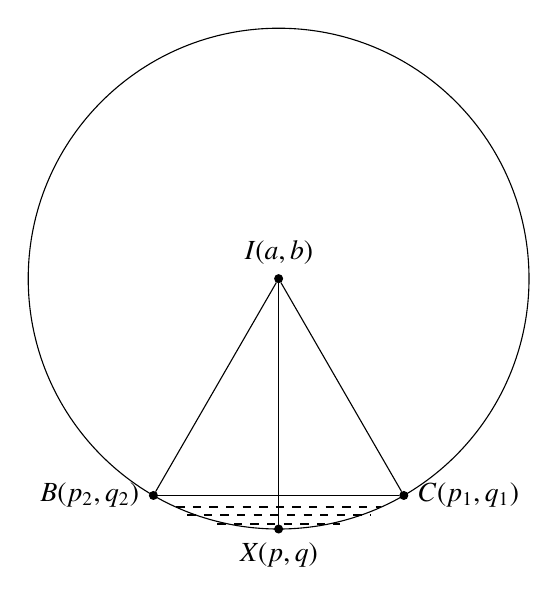
\begin{tikzpicture}
[
scale =2,
>=stealth,
point/.style = {draw, circle, fill = black, inner sep = 1pt},
]

\def\rad{1.59}
\coordinate [point, label={above : $I{(a,b)}$ }] (I) at (0, 0);
\draw (I) circle (\rad);

\node (C) at (300:{\rad})[point,label = right:$C{(p_1,q_1)}$] {};

\node (X) at (270:{\rad}) [point,label = below:$X{(p,q)}$] {};

\node (B) at (240:{\rad}) [point,label = left:$B{(p_2,q_2)}$] {};

\draw (C) -- (I);
\draw (B) -- (I);
\draw (B) -- (C);
\draw (I) -- (X);

\draw[black,thick,dashed](-0.65,-1.45) -- (0.65,-1.45);
\draw[black,thick,dashed](-0.58,-1.5) -- (0.58,-1.5);
\draw[black,thick,dashed](-0.39,-1.56) -- (0.39,-1.56);
\end{tikzpicture}

%}
%\caption{Notion of the derivative.}
%\label{fig:derivative}
%\end{figure}
\\
\solution Let $\vec{x}_1,\vec{x}_2$ be two points on the circle such that 
$x_1x_2 \parallel BC$. Then
%
\begin{align}
\norm{\vec{x}_1-\vec{I}}^2- 
\norm{\vec{x}_2-\vec{I}}^2 &= 0 
\\
\implies 
\brak{\vec{x}_1-\vec{x}_2}^T\brak{\frac{\vec{x}_1+\vec{x}_2}{2}-\vec{I}} &= 
0 
\\
\implies 
\brak{\vec{B}-\vec{C}}^T\brak{\frac{\vec{x}_1+\vec{x}_2}{2}-\vec{I}} &= 
0 
%\label{eq:circle_bisect}
\end{align}
%
For $\vec{x}_1=\vec{x}_2=\vec{U}$, $x_1x_2$ merges into $BC$ and the above 
equation becomes 
%
\begin{align}
\brak{\vec{B}-\vec{C}}^T\brak{\vec{U}-\vec{I}} = 
0 
\implies OD \perp BC
%\label{eq:circle_bisect}
\end{align}
%
\item Give an alternative proof for the above.
\\
\solution Let 
\begin{align}
\vec{B} & = \mbf{0}
\\
\vec{U} &= \lambda \vec{m}
\end{align}
Then
\begin{align}
\norm{\vec{U} - \vec{I}}^2 = r^2 &
\\
\implies \lambda^2\norm{\vec{m}}^2 - 2\lambda\vec{m}^T\vec{I} + \norm{\vec{I}}^2 &= r^2 
\end{align}
Since the above equation has a single root,
\begin{align}
\lambda = \frac{\vec{m}^T\vec{I}}{\norm{\vec{m}}^2}
\label{eq:incircle_lam}
\end{align}
%
Thus, 
\begin{align}
\brak{\vec{U} - \vec{B}}^T\brak{\vec{U} - \vec{I}}
&= \brak{\lambda\vec{m}}^T
\brak{\lambda\vec{m}-\vec{I}}
\\
&=\lambda^2\norm{\vec{m}}^2-\lambda\vec{m}^T\vec{I}
\\
&= \mbf{O} \text{ (from \ref{eq:incircle_lam})}.
\\
\implies & OD \perp BC
\end{align}
\item Find the equation of the tangent at $\vec{U}$.
\\
\solution The equation of the tangent is given by 
\begin{align}
\brak{\vec{I}-\vec{U}}^T\brak{\vec{x}-\vec{U}}=0
%\label{eq:circle_bisect}
\end{align}
%
\item The direction vector of {\em normal to the circle}  in \eqref{eq:circ_quad} at point $\vec{U}$ is
\begin{align}
\label{eq:circ_normal}
\vec{n} = \vec{U}-\vec{I}
\end{align}
%
%where $k$ is a constant.
\item Find an expression for $r$ if $\vec{I}$ is known.
\\
\solution Let $\vec{n}$ be the normal vector of $BC$.  The equation for $BC$ is then given by
\begin{align}
\vec{n}^T\brak{\vec{x}-\vec{B}} &= 0
\\
\implies \vec{n}^T\brak{\vec{U}-\vec{B}} &= 0
\label{eq:incirc_ub}
\end{align}
since $\vec{U}$ lies on $BC$.
Since $IU \perp BC$, 
\begin{align}
\label{eq:incirc_iu}
\vec{I}&=\vec{U}+\lambda\vec{n}
\\
\implies \vec{I}-\vec{U}&=\lambda\vec{n}
\\
\text{or}\quad r=\norm{\vec{I}-\vec{U}}&=\abs{\lambda}\norm{\vec{n}}
\label{eq:incirc_r}
\end{align}
From \eqref{eq:incirc_ub} and \eqref{eq:incirc_iu}
\begin{align}
\vec{n}^T\vec{I}&=\vec{n}^T\vec{B}+\lambda\vec{n}^T\vec{n}
\\
\implies \vec{n}^T\brak{\vec{I}-\vec{B}}&=\lambda\norm{\vec{n}}^2
\\
\implies r = \abs{\lambda}\norm{\vec{n}}&=\frac{\abs{\vec{n}^T\brak{\vec{I}-\vec{B}}}}{\norm{\vec{n}}}
\end{align}
from \eqref{eq:incirc_r}.  Letting 
\begin{align}
\norm{\vec{n}_1}&= \frac{\vec{n}}{\norm{\vec{n}}},
\\
r &= \abs{\vec{n}_1^T\brak{\vec{I}-\vec{B}}}
\label{eq:incirc_rad}
\end{align}
\item Find $\vec{I}$.
\\
\solution Since $r = IU = IV = IW$, from \eqref{eq:incirc_rad},
\begin{align}
\abs{\vec{n}_1^T\brak{\vec{I}-\vec{B}}} = \abs{\vec{n}_2^T\brak{\vec{I}-\vec{C}}} = 
\abs{\vec{n}_3^T\brak{\vec{I}-\vec{A}}}
\label{eq:incirc_radeq}
\end{align}
%
where $\vec{n}_2, \vec{n}_3$ are unit normals of $CA, AB$ respectively.  \eqref{eq:incirc_radeq} can be 
expressed as 
\begin{align}
\vec{n}_1^T\brak{\vec{I}-\vec{B}} &= k_1\vec{n}_2^T\brak{\vec{I}-\vec{C}} 
\\
\vec{n}_2^T\brak{\vec{I}-\vec{C}} &= k_2\vec{n}_3^T\brak{\vec{I}-\vec{A}}
\label{eq:incirc_k1k2}
\end{align}
%
where $k_1,k_2 = \pm 1$. The above equations can be expressed as the matrix equation
\begin{align}
\myvec{\vec{n}_1-k_1\vec{n}_2 & \vec{n}_2 - k_2\vec{n}_3}^T\vec{I} &= 
\myvec{\vec{n}_1^T\vec{B}-k_1\vec{n}_2^T\vec{C} \\ \vec{n}_2^T \vec{C} - k_2\vec{n}_3^T\vec{A}}
\label{eq:incirc_k1k2fin}
\end{align}
\item Show that $\vec{I}$ lies inside $\triangle ABC$ for $k_1=k_2=1$
%\label{eq:line_dist_pt}
\item Let $a = BC, b = CA$, $ c= AB$, $x = BU=BW$, $y = CU=CV$, $z = AV=AW$. Find $\vec{U}$.
\\
\solution It is easy to verify that 
\begin{align}
\label{eq:incircle_mat}
\myvec{1 & 1 & 0\\0 & 1 & 1\\1 & 0 & 1}\myvec{x\\y\\z} = \myvec{a\\b\\c}
\end{align}
%
which can be used to obtain $x$ and $y$.
Using the section formula, 
\begin{align}
\vec{U} = \frac{x\vec{B}+\vec{A}}{x+y}
\end{align}

\item Show that the angle in a semi-circle is a right angle.
\begin{figure}[!h]
\centering
\resizebox {\columnwidth} {!} {
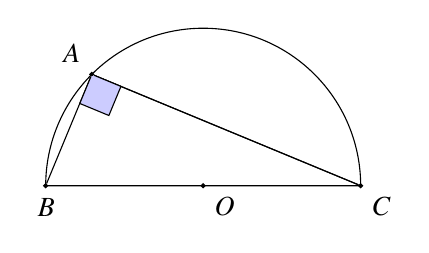
\begin{tikzpicture}
  [
    scale=2,
    >=stealth,
    point/.style = {draw, circle,  fill = black, inner sep = 0.5pt},
    dot/.style   = {draw, circle,  fill = black, inner sep = .2pt},
  ]

 \coordinate [point, label={below :	$B$ }] (B) at (-1, 0);
 \coordinate [point, label={below right:	$O$ }] (O) at (0, 0);
 \coordinate [point, label={below right:	$C$ }] (C) at (1, 0); 
 \coordinate [point, label={above left:	$A$ }] (A) at (-0.707,0.707);  
\draw (A) -- (C) arc(0:180:1) --cycle;
  \draw 
  (A) -- (B)
  (A) -- (C);
  \tkzMarkRightAngle[fill=blue!20,size=.2](B,A,C)    
%  \def\rad{1}

%  \draw (O) circle (\rad);  
%    \node (A) at +(45:{\rad}) [point,label = above right:$A$ $\brak{x,y}$] {};  
%  \path
%     (O)    edge  node[sloped, anchor=center, below, text width=0.5cm] { $r$}     (A) ; 
    
% \coordinate [point, label={below left:$B$}] (B) at (0, 0);
%    \node (A) at +(60:{2*sqrt(3)}) [label = above:$A$] {};
%  \coordinate [ label={below right:$C$ }] (C) at ($ (3,0) + sqrt(3)*(1,0) $);
%    \node (P) at +(30:{2*sqrt(3)}) [label = above:$P$] {};  
%  \path[->]
%     (B)    edge  node[sloped, anchor=center, below, text width=2.0cm] { $y = m_1x+c_1$}     (A) 
%	 (B)    edge  node[sloped, anchor=east, below, text width=2.0cm] { $y=m_2x+c_2$}     (C)
%	 (B)    edge  node[sloped, anchor=east, below, text width=2.0cm] { Bisector}     (P);
%  
%%  
%%  \coordinate [point, label={below left:$B$ $\brak{0,0}$}] (B) at (0, 0);
%%    \node (A) at +(60:{2*sqrt(3)}) [point, label = above:$A$ $\brak{a,b}$] {};
%%  \coordinate [point, label={below right:$C$ $\brak{c,0}$}] (C) at ($ (3,0) + sqrt(3)*(1,0) $);
%%  \node (D) at ({sqrt(3)},0) [point, label = below:$D$ $\brak{a,0}$] {};
%%    \node (E) at +(45:{(3+sqrt(3))/sqrt(2)}) [point, label = above right:$E$] {};
%%    \node (O) at +(45:{sqrt(6)}) [point, label = right:$O$] {};    
%%    \node (F) at +(60:{(3+sqrt(3))/2}) [point, label = left:$F$] {};        
%  \draw  (A) -- (B) -- (C);% -- (A);
%%  \node (D) at ($(B)!0.5!(C)$) [point, label = {below:$D$}]{};
%%  \draw (A) -- (D);  
%%  \draw (B) -- (E);    
%%  \draw[dashed] (C) -- (F);      
%\tkzMarkAngle[draw = black, fill = white, opacity=1](P,B,A)
%\tkzLabelAngle[pos = 0.8](P,B,A){$\theta$}
%\tkzMarkAngle[draw = black, fill = white, opacity=1,size=1.1](C,B,P)
%\tkzLabelAngle[pos = 0.9](C,B,P){$\theta$}

%\tkzMarkAngle[size=1.4,draw = black, fill = white, opacity=1](C,B,P)
%\tkzLabelAngle[pos=1.15,font=\scriptsize](C,B,P){$\theta$}

%  \tkzMarkAngle[fill=white,opacity=1,size=0.2,label={$\theta$},pos=0.2](P,B,A)  
%  \tkzMarkAngle[fill=blue!20,size=.4,label={$\theta$}](P,B,A)
%  \tkzMarkAngle[fill=blue!20,size=.2,label={$\theta$](C,B,P)
%  \tkzMarkRightAngle[fill=blue!20,size=.2](B,E,A)  
%  \path
%     (B)    edge  node[sloped, anchor=center, below, text width=2.0cm] { $k_1:1$}     (E)  
%	 (C)    edge  node[sloped, anchor=east, below, text width=2.0cm] { $1:k_2$}     (F);

\end{tikzpicture}


}
\caption{Angle in a semi-circle.}
\label{fig:ch2_line}
\end{figure}
\\
\solution Let 
\begin{align}
\vec{O} = 0
\end{align}
From the given information,
\begin{align}
\label{eq:semi_circ_pt}
\norm{\vec{A}}^2 = \norm{\vec{B}}^2 = \norm{\vec{C}}^2 = r^2
\\
\norm{\vec{B}-\vec{C}}^2 =  \brak{2r}^2
\\
\vec{B} + \vec{C} = 0
\label{eq:semcirc_mid}
\end{align}
%
where $r$ is the radius of the circle. Thus,
\begin{multline}
\norm{\vec{A}-\vec{B}}^2 + \norm{\vec{A}-\vec{C}}^2 = 
2\norm{\vec{A}}^2 + \norm{\vec{B}}^2 + \norm{\vec{C}}^2
\\
-2\vec{A}^T\brak{\vec{B}+\vec{C}}
%\\
%\norm{\vec{B}-\vec{C}}^2 =  \brak{2r}^2
%\\
%\vec{B} + \vec{C} = 0
\end{multline}
From \eqref{eq:semcirc_mid} and \eqref{eq:semi_circ_pt},
\begin{multline}
\norm{\vec{A}-\vec{B}}^2 + \norm{\vec{A}-\vec{C}}^2 = 4r^2 = \norm{\vec{B}-\vec{C}}^2 
%\\
%\norm{\vec{B}-\vec{C}}^2 =  \brak{2r}^2
%\\
%\vec{B} + \vec{C} = 0
\end{multline}
Thus, using Baudhayana's theorem, $\triangle ABC$ is right angled.
\item 	Show that $PA.PB = PC^2$, where $PC$ is the tangent to the circle in Fig. \ref{fig:tangent_secant}.

	\begin{figure}[!hb]
		\begin{center}
			
			%\includegraphics[width=\columnwidth]{./figs/ch4_tangent_prod}
			%\vspace*{-10cm}
			\resizebox{\columnwidth}{!}{\begin{tikzpicture}
[scale =2,>=stealth,point/.style = {draw, circle, fill = black, inner sep = 1pt},]

\def\rad{2}
\coordinate [point, label={above: $O$ }] (O) at (0, 2);
\draw (O) circle (\rad);
\node (P) at (-4,0)[point,label=below :$P$] {};
\node (C) at (0,0)[point,label=below :$C$] {};
\node (A) at (-1.92,1.45)[point,label=above left :$A$] {};
\node (B) at (1.2,3.6)[point,label=above right :$B$] {};
\draw (O)--(P);
\draw (P)--(C);
\draw (P)--(B);
%\draw (A)--(O);
%\draw (B)--(C);

\draw [thick,dashed](A)--(O);
\draw [thick,dashed](C)--(O);
\draw [thick,dashed](B)--(O);
%\tkzMarkRightAngle[size=.2](P,C,O);
%\tkzMarkAngle[size=.3](A,B,C);
%\tkzMarkAngle[size=.4](O,C,A);
%\tkzMarkAngle[size=.5](B,C,O);
%\tkzMarkAngle[size=.3](P,A,C);
%\tkzMarkAngle[size=.2](C,A,O);
%\tkzMarkAngle[size=.2](A,O,C);
%
\node [above] at (0.35,2.5){$r$};
\node [above] at (-0.9,1.7){$r$};
\node [above] at (0.1,1.0){$r$};
%\draw (-1.9,1) node{$\theta$};

%\draw (0.95,3.3) node{$\alpha$};
%\draw (-0.2,1.7) node{$2\alpha$};
%\draw (-0.2,0.5) node{$90-\alpha$};
%\draw (-1.4,1.4) node{$90-\alpha$};
%\draw (.1,.6) node{$\phi$};

\end{tikzpicture}}
		\end{center}
		\caption{$PA.PB = PC^2$.}
		\label{fig:tangent_secant}	
	\end{figure}
\solution Let $\vec{P} = \mbf{0}$.  Then, we have the following equations
\begin{align}
\label{eq:tan_sec_AB}
PA.PB &= \lambda \norm{\vec{A}}^2 \quad \because (\vec{B} = \lambda \vec{A})
\\
\norm{\vec{A}-\vec{O}}^2 &= \norm{\vec{B}-\vec{O}}^2 = \norm{\vec{C}-\vec{O}}^2 = r^2
\\
\norm{\vec{O}}^2-\norm{\vec{C}}^2 &=  r^2 \quad \triangle PCO\text{ is 
right angled}
\label{eq:tan_sec_boudh}
\end{align}
$\because$
\begin{align}
%\label{eq:tan_sec_AB}
%PA.PB &= \lambda \norm{\vec{A}}^2 \quad \because (\vec{B} = \lambda 
%\vec{A})
%\\
\norm{\vec{B}-\vec{O}}^2-\norm{\vec{A}-\vec{O}}^2   &=0,
\\
\brak{\lambda^2-1}\norm{\vec{A}}^2 - 2 \brak{\lambda-1}\vec{A}^T\vec{O} &= 
0
\\
\implies PA.PB = \lambda\norm{\vec{A}}^2 =  2 
\vec{A}^T\vec{O}-\norm{\vec{A}}^2 &
%\norm{\vec{C}-\vec{O}}^2 = r^2
%\\
%\norm{\vec{O}}^2-\norm{\vec{C}}^2 &=  r^2 \quad \triangle PCO\text{ is 
%right angled}
%\label{eq:tan_sec_boudh}
\label{eq:tan_sec_first}
\end{align}
after substituting from \eqref{eq:tan_sec_AB} and simplifying. From 
\eqref{eq:tan_sec_boudh},
\begin{align}
\norm{\vec{A}-\vec{O}}^2 = \norm{\vec{O}}^2-\norm{\vec{C}}^2  &= r^2
\\
\implies 2 \vec{A}^T\vec{O}-\norm{\vec{A}}^2   = \norm{\vec{C}}^2 = PC^2&
\label{eq:tan_sec_second}
\end{align}
From \eqref{eq:tan_sec_first} and \eqref{eq:tan_sec_second},
\begin{align}
PA.PB = PC^2
\end{align}

\item In Fig. \ref{fig:chords} show that $PA.PB = PC.PD$.
\begin{figure}[!ht]
	\begin{center}
		
		%\includegraphics[width=\columnwidth]{./figs/ch3_angle_bisector}
		%\vspace*{-10cm}
		\resizebox{\columnwidth}{!}{\begin{tikzpicture}
[scale=2,>=stealth,point/.style={draw,circle,fill = black,inner sep=0.5pt},]
%\node (D) at (0, 0)[point,label=below :$D$] {};
\node (B) at (-2, -2)[point,label=below left :$C$]{};
\node (A) at (1, 3)[point,label=above:$A$]{};
\node (C) at (4, -1)[point,label=below right:$B$]{};
%\coordinate [point, label={above : $O$ }] (I) at  (1.147, 1.143);
\node (O) at (0.7962963,-0.27777778)[point,label=above:$O$]{};
\node (D) at (  3.64041158, 1.36427295)[point,label=below:$D$]{};
\node (P) at ( 2.66371481, 0.78171359)[point,label=right:$P$]{};
%\node (x1) at (0.601,-1.357)[point,label=left:$x_1$]{};
%\node (x2) at (2.15,-1.1)[point,label=right:$x_2$]{};
%\node (temp) at ($(O)!0.5!(D)$)[label=right:$r$]{};
%\node (D) at (2.424,1.1)[point,label=above right:$D$]{};
%\node (E) at (1.1, 1.9)[point,label=above right:$E$]{};
%\node (F) at (-1.1, 1.9)[point,label=above left:$F$]{};
\def\rad{3.284101453883}
\draw (O) circle (\rad);

%\draw (D)--(O);
%\draw (A)--(B);
\draw (B)--(D);
\draw (A)--(C);
%\draw (C)--(D);
%\draw [thick,dashed] (x1) -- (x2);
%\draw [thick,dashed] (O) -- (E);
%\draw [thick,dashed] (O) -- (F);
%\draw (B)--(O);
%\draw (C)--(O);

%\tkzMarkRightAngle[size=.2](A,D,C)
%\tkzMarkRightAngle[size=.15](B,F,O);
%\tkzMarkRightAngle[size=.15](C,E,O);
%\tkzMarkAngle[size=.4](D,B,O);
%\tkzMarkAngle[size=.35](O,B,F);
%\tkzMarkAngle[size=.54](E,C,O);
%\tkzMarkAngle[size=.5](E,C,O);
%\tkzMarkAngle[size=.6](O,C,D);
%\tkzMarkAngle[size=.65](O,C,D);

\end{tikzpicture}}
	\end{center}
	\caption{Chords of a circle}
	\label{fig:chords}	
\end{figure}
\\
\solution Let $\vec{P} = \mbf{0}$.  We then have the following equations
\begin{align}
\begin{split}
\vec{B} &= k_1 \vec{A}, k_1 = \frac{PB}{PA}
\\
\vec{D} &= k_2 \vec{C}, k_2 = \frac{PD}{PC}
\end{split}
\label{eq:chords_ratio}
\\
\begin{split}
\norm{\vec{A}-\vec{O}}^2 &= \norm{\vec{B}-\vec{O}}^2 
\\
= \norm{\vec{C}-\vec{O}}^2 &= \norm{\vec{D}-\vec{O}}^2 = r^2
\end{split}
\label{eq:chords_points}
\end{align}
%
where $r$ is the radius of the circle and $\vec{O}$ is the centre. From \eqref{eq:chords_points},
\begin{align}
&\norm{\vec{A}-\vec{O}}^2 = \norm{\vec{B}-\vec{O}}^2
\\
\implies &\norm{\vec{A}-\vec{O}}^2 = \norm{k\vec{A}-\vec{O}}^2 \quad(\text{from \eqref{eq:chords_ratio}})
\end{align}
%
which can be simplified to obtain
\begin{align}
k_1\norm{\vec{A}}^2 = 2\vec{A}^T\vec{O}-\norm{\vec{A}}^2
\label{eq:chords_Anorm}
\end{align}
Similarly,
\begin{align}
k_2\norm{\vec{C}}^2 = 2\vec{C}^T\vec{O}-\norm{\vec{C}}^2
\label{eq:chords_Cnorm}
\end{align}
%
From \eqref{eq:chords_points}, we also obtain
\begin{align}
\norm{\vec{A}-\vec{O}}^2 
= \norm{\vec{C}-\vec{O}}^2 
\\
\implies 2\vec{A}^T\vec{O}-\norm{\vec{A}}^2 = 2\vec{C}^T\vec{O}-\norm{\vec{C}}^2
\label{eq:chords_ACnorm}
\end{align}
%
after simplification. Using this result in \eqref{eq:chords_Anorm} and \eqref{eq:chords_Cnorm},
\begin{align}
k_1\norm{\vec{A}}^2 = k_2\norm{\vec{C}}^2
\\
\implies \norm{\vec{A}}\, \norm{\vec{B}}=\norm{\vec{C}}\,\norm{\vec{D}}
\end{align}
which completes the proof.

\item (Pole and Polar:) The polar of a point $\vec{x}$ with respect to the curve
\begin{align}
\label{eq:quad_form_polar}
\vec{x}^T\vec{V}\vec{x}+2\vec{u}^T\vec{x}+f=0
\end{align}
is the line
\begin{align}
\label{eq:polar}
\vec{n}^T\vec{x} = c
\end{align}
%
where
\begin{align}
\myvec{\vec{n}^T\\ - c}=
\myvec{
\vec{V}&\vec{u}
\\
\vec{u}^T&f
}
\myvec{\vec{x}\\1}
\end{align}
%
The pole of the line  in \eqref{eq:polar} is obtained as $\frac{1}{x_3}\myvec{x_1\\x_2}$, where
\begin{align}
\myvec{x_1 \\ x_2\\x_3}
=\myvec{
\vec{V}&\vec{u}
\\
\vec{u}^T&f
}^{-1}
\myvec{\vec{n}^T\\ - c}
\end{align}
\item $\vec{x}_1$ and $\vec{x}_2$ are said to be conjugate points for \eqref{eq:quad_form_polar} if $\vec{x}_2$ lies on the polar of $\vec{x}_1$ and vice-versa.  A similar definition holds for conjugate lines as well.
\item Let $\vec{p}$ be a point of intersection of two circles with centres $\vec{c}_1$ and $\vec{c}_2$.  The circles are said to be orthogonal if their tangents at $\vec{p}$ are perpendicular to each other.  Show that if $r_1$ and $r_2$ are their respective radii, 
\begin{align}
\label{eq:circ_orth}
\norm{\vec{c_1}-\vec{c}_2}^2 = r_1^2+r_2^2 
\end{align}
\item Show that the length of the tangent from a point $\vec{p}$ to the circle 
\begin{align}
\label{eq:circ_quad_len}
\vec{x}^T\vec{x}-2\vec{c}^T\vec{x} + f = 0
\end{align}
%
is 
\begin{align}
\label{eq:circ_tang_len}
\vec{p}^T\vec{p}-2\vec{c}^T\vec{p} + f 
\end{align}
This length is also known as the {\em power} of the point $\vec{p}$ with respect to the circle.
\item  The {\em radical axis} of the circles 
\begin{align}
%\label{eq:circs_two}
\vec{x}^T\vec{x}-2\vec{c}_1^T\vec{x} + f_1 = 0
\\
\vec{x}^T\vec{x}-2\vec{c}_2^T\vec{x} + f_2 = 0
\end{align}
%
is the locus of the points from which lengths of the tangents to the circles are equal.  From \eqref{eq:circs_two}, this locus is
\begin{align}
\vec{x}^T\vec{x}-2\vec{c}_1^T\vec{x} + f_1 -
%\nonumber \\
\vec{x}^T\vec{x}-2\vec{c}_2^T\vec{x} + f_2 = 0
\\
\implies 2\brak{\vec{c}_1-\vec{c}_2}^T\vec{x} + f_2 - f_1 = 0
\label{eq:circs_rad_axis}
\end{align}
\item Show that the radical axis of the circles is perpendicular to the line joining their centres.\item {\em Coaxal circles} have the same radical axis.
\item Obtain a family of coaxal circles from \label{eq:circs_two} and find their {\em limit points}.
\\
\solution The family of circles is obtained as
\begin{align}
\label{eq:circs_coaxal_family}
\vec{x}^T\vec{x}-2\brak{\vec{c}_1 +\lambda\vec{c}_2}^T\vec{x} + f_1 +\lambda f_2= 0
\end{align}
%
The limit points are the centres of those circles whose radii are 0. From \eqref{eq:circs_coaxal_family} and \eqref{eq:circ_quad},
this results in
\begin{align}
%\label{eq:circs_coaxal_family}
f_1 +\lambda f_2 =  \brak{\vec{c}_1 +\lambda\vec{c}_2}^T\brak{\vec{c}_1 +\lambda\vec{c}_2} &
\\
\implies \lambda^2 \norm{\vec{c}_2}^2 + \lambda \brak{2\vec{c}_1^T\vec{c}_2-f_2} + \norm{\vec{c}_1}^2-f_1 = 0&
\end{align}
Solving for $\lambda$, the limit points are given by  
\begin{align}
\vec{c}_1+\lambda\vec{c}_2
\end{align}
\end{enumerate}



\subsection{Programming}
\renewcommand{\theequation}{\theenumi}
\begin{enumerate}[label=\arabic*.,ref=\thesubsection.\theenumi]
\numberwithin{equation}{enumi}

\item Find the circumcentre $\vec{O}$ and radius $R$ of $\triangle ABC$ in Fig. \ref{fig:triangle}
\\
\solution $\vec{O}$ can be obtained from 
%
The following code computes $\vec{O}$ using \eqref{eq:defs_ccircle_c1} and \eqref{eq:defs_ccircle_c2}
\begin{lstlisting}
codes/2d/circumcentre.py
\end{lstlisting}
\item Plot the circumcircle of $\triangle ABC$.
\\
\solution The following code plots Fig. \ref{fig:circumcircle}
\begin{lstlisting}
codes/2d/circumcircle.py
\end{lstlisting}
\begin{figure}
\centering
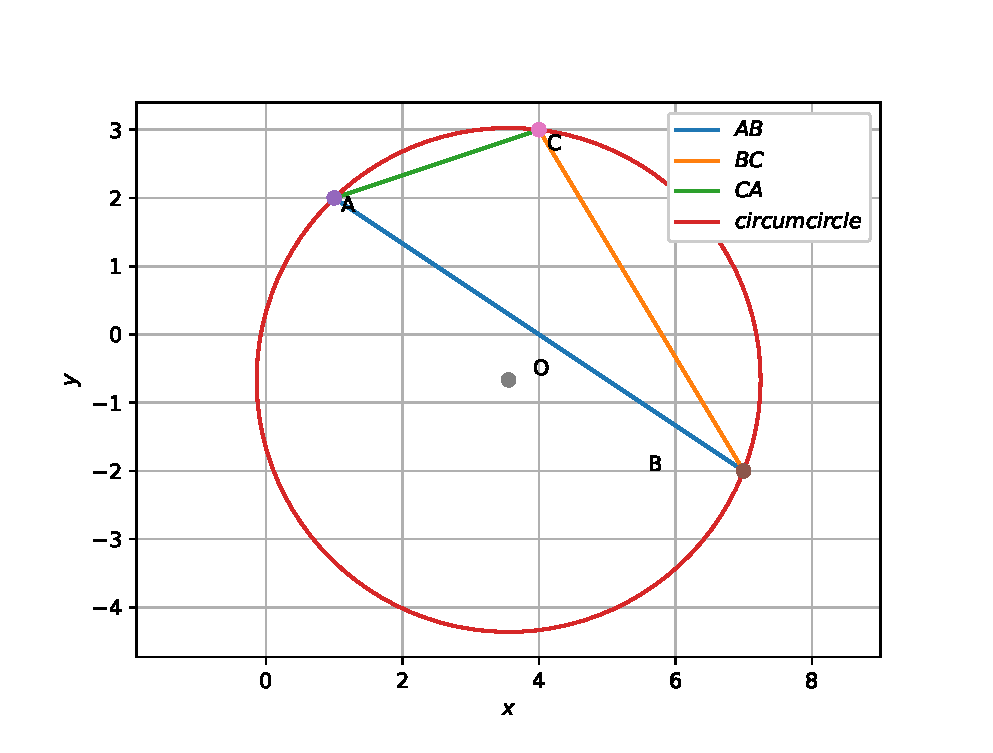
\includegraphics[width=\columnwidth]{./circle/figs/circumcircle.eps}
\caption{}
\label{fig:circumcircle}
\end{figure}


\item Consider a circle with centre $\vec{I}$ and radius $r$ that lies within $\triangle ABC$ and touches 
$BC, CA$ and $AB$ at $\vec{U}, \vec{V}$ and $\vec{W}$ respectively.

\item Compute $\vec{I}$ and $r$.
\\
\solution The following code uses \eqref{eq:incirc_k1k2fin}  and \eqref{eq:incirc_rad} to compute $\vec{I}$ and  $r$ respectively.


\begin{lstlisting}
codes/2d/incentre.py
\end{lstlisting}
\item Plot the incircle of $\triangle ABC$
\\
\solution The following code plots the incircle in Fig. \ref{fig:incircle}
\begin{lstlisting}
codes/2d/incircle.py
\end{lstlisting}
\begin{figure}
\centering
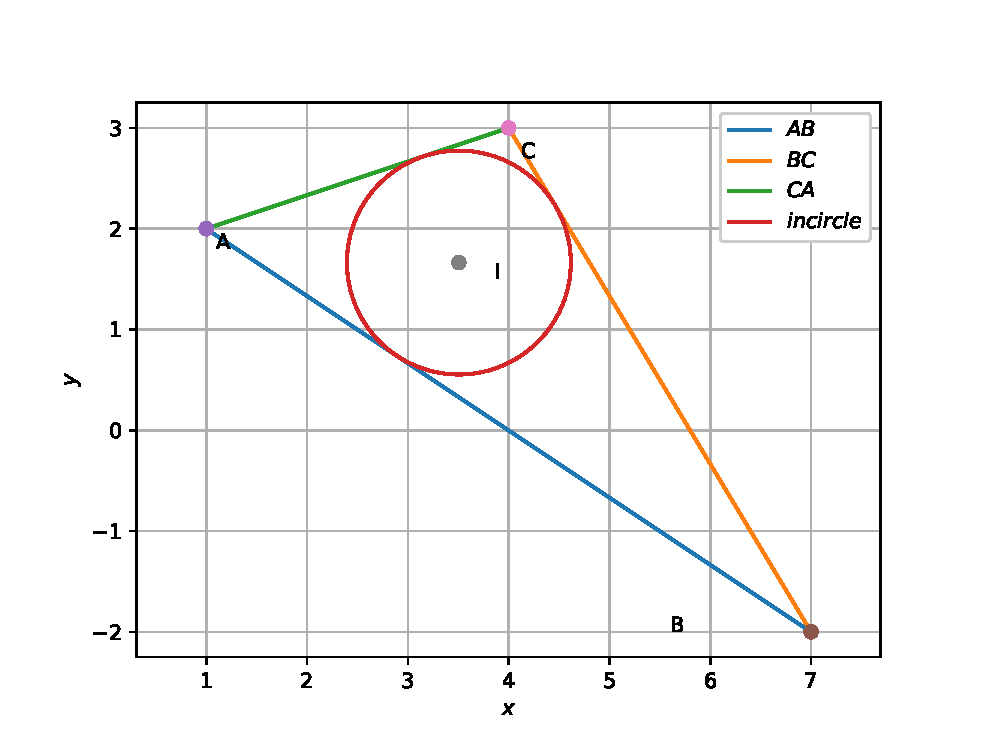
\includegraphics[width=\columnwidth]{./circle/figs/incircle.eps}
\caption{}
\label{fig:incircle}
\end{figure}

\end{enumerate}



\subsection{Example}
\renewcommand{\theequation}{\theenumi}
\begin{enumerate}[label=\arabic*.,ref=\thesubsection.\theenumi]
\numberwithin{equation}{enumi}
\item Find the centre and radius of the circle
\begin{equation}
C_1: \vec{x}^T\vec{x} - \myvec{2 & 0}\vec{x} 
-1 = 0 
\label{eq:circle_c1}
\end{equation}
%
\\
\solution let $\vec{c}$ be the centre of the circle.  Then
\begin{align}
\norm{\vec{x}-\vec{c}}^2 &= r^2
\\
\implies \brak{\vec{x}-\vec{c}}^T\brak{\vec{x}-\vec{c}} &= r^2
\\
\implies \vec{x}^T\vec{x} - 2\vec{c}^T\vec{x} &= r^2-\vec{c}^T\vec{c}
\end{align}
%
Comparing with \eqref{eq:circle_c1},
\begin{align}
\vec{c} &= \myvec{1 \\0}
\\
r^2-\vec{c}^T\vec{c} &= 1 \implies r = \sqrt{2}
\end{align}

\item Find the tangent to the circle $C_1$
at the point $\myvec{2 \\1}$.
\\
\solution From \eqref{eq:tangent}, the tangent $T$ is given by
\begin{align}
\sbrak{\myvec{2 & 1}-\myvec{1 & 0}}\vec{x} -\myvec{2 & 1}\myvec{1 \\ 0}  &= 1
\\
\implies T: \vec{n}^T\vec{x}   &= 3
\label{eq:circle_tangent}
\end{align}
%
where
\begin{equation}
\vec{n}=\myvec{1 \\ 1}
\end{equation}
\item The tangent $T$ in \eqref{eq:circle_tangent} cuts off a chord $AB$
from a circle $C_2$ whose 
centre is 
\begin{equation}
\vec{C}=\myvec{3 \\ 
-2}. 
\end{equation}
Find $\vec{A}+ \vec{B}$.
\\
\solution Let the radius of $C_2$ be $r$.  From the given information,
\begin{align}
\brak{\vec{A}-\vec{C}}^T\brak{ \vec{A}-\vec{C} } &= r^2
\label{eq:circle_x1}
\\
\brak{\vec{B}-\vec{C}}^T\brak{ \vec{B}-\vec{C} } &= r^2
\label{eq:circle_x2}
\end{align}
%
 Subtracting 
\eqref{eq:circle_x2} from \eqref{eq:circle_x1},
\begin{flalign}
&\vec{A}^T \vec{A}-\vec{B}^T \vec{B}-2\vec{C}^T\brak{\vec{A}- \vec{B}}  = 0
\\
&\implies \brak{\vec{A}+\vec{B}}^T\brak{ \vec{A}-\vec{B} }-2\vec{C}^T\brak{\vec{A}- \vec{B}} = 0
\nonumber \\
&\implies  \brak{\vec{A}+\vec{B}-2\vec{C}}^T\brak{ \vec{A}-\vec{B} } = 0
\label{eq:circle_aborth}
\end{flalign}
 $\because \vec{A},\vec{B}$ lie on $T$, from \eqref{eq:circle_tangent},
\begin{align}
\label{eq:circle_abtangent}
\vec{n}^T\vec{A} = \vec{n}^T\vec{B}   &= 3
\\
\implies \vec{n}^T\brak{\vec{A} -\vec{B}}   &= 0,
\label{eq:circle_north}
\end{align}
From \eqref{eq:circle_aborth} and \eqref{eq:circle_north}
\begin{align}
\label{eq:circle_abkn}
\vec{A}+\vec{B}-2\vec{C} &= k\vec{n}
\\
\implies \vec{n}^T\vec{A}+\vec{n}^T\vec{B}-2\vec{n}^T\vec{C} &= k\vec{n}^T\vec{n}
\\
\implies \frac{\vec{n}^T\vec{A}+\vec{n}^T\vec{B}-2\vec{n}^T\vec{C}}{\vec{n}^T\vec{n}} &= k
\\
\implies k &= 2
\end{align}
using \eqref{eq:circle_abtangent}.
Substituting in \eqref{eq:circle_abkn}
\begin{align}
\vec{A}+\vec{B} &= 2\brak{\vec{n}+\vec{C}}
\label{eq:circle_a+b}
\end{align}
%
\item If $AB = 4$, find $\vec{A}^T\vec{B}$.
%
\\
\solution From the given information,
\begin{align}
\norm{\vec{A}-\vec{B}}^2 &= 4^2
\end{align}
resulting in
\begin{align}
\norm{\vec{A}+\vec{B}}^2-\norm{\vec{A}-\vec{B}}^2 &= 4\norm{\vec{n}+\vec{C}}^2-4^2
\\
\implies\vec{A}^T\vec{B} &= \norm{\vec{n}+\vec{C}}^2-4 = 17
\end{align}
using \eqref{eq:circle_a+b} and simplifying.
%
\item Show that
\begin{equation}
\label{eq:circle_acb}
\brak{\vec{A}-\vec{C}}^T\brak{\vec{B}-\vec{C}} =8 - r^2
\end{equation}
\\
\solution
\begin{align}
\norm{\vec{A}-\vec{B}}^2 &= 4^2
\\
\implies\brak{\vec{A}-\vec{B}}^T\brak{ \vec{A}-\vec{B} } &= 4^2
\label{eq:circle_x1x2}
\end{align}
%
From \eqref{eq:circle_x1x2},
\begin{align}
\sbrak{\brak{\vec{A}-\vec{C}}-\brak{\vec{B}- \vec{C}}}^T\sbrak{ 
\brak{\vec{A}-\vec{C}}-\brak{\vec{B}- \vec{C}}} = 4^2
\end{align}
%
which can be expressed as
\begin{align}
\norm{\vec{A}-\vec{C}}^2+\norm{\vec{B}-\vec{C}}^2 &
+ 2\brak{\vec{A}-\vec{C}}^T\brak{\vec{B}-\vec{C}} 
= 4^2
\end{align}
Upon substituting from \eqref{eq:circle_x2} and  \eqref{eq:circle_x1} and simplifying, \eqref{eq:circle_acb}
is obtained.
\item Find $r$.
\\
\solution \eqref{eq:circle_acb} can be expressed as
\begin{align}
 \vec{A}^T\vec{B}  -\vec{C}^T\brak{\vec{A}+\vec{B}}+\vec{C}^T\vec{C} &=8 - r^2
\\
\implies 8 - \vec{A}^T\vec{B}  +\vec{C}^T\brak{\vec{A}+\vec{B}}-\vec{C}^T\vec{C} &= r^2
\\
\implies 8 - \vec{A}^T\vec{B}  +\vec{C}^T\brak{2\vec{n}+\vec{C}} &= r^2
\\
\implies r =  \sqrt{6}.
\end{align}
\item Summarize all the above computations through a Python script and plot 
the tangent and circle.
\\
\solution The following code generates Fig. \ref{fig:circle}.
\begin{lstlisting}
wget 
codes/2d/circ.py
\end{lstlisting}
\begin{figure}
\centering
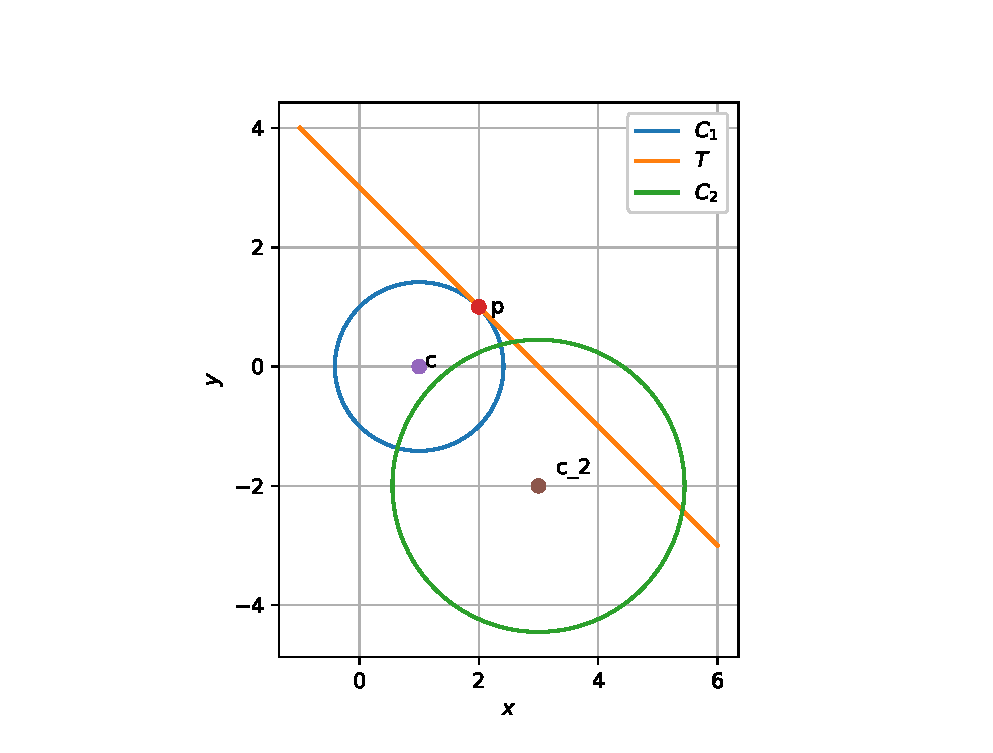
\includegraphics[width=\columnwidth]{./circle/figs/circle.eps}
\caption{}
\label{fig:circle}
\end{figure}

\end{enumerate}



\subsection{Lagrange Multipliers}
\renewcommand{\theequation}{\theenumi}
\begin{enumerate}[label=\arabic*.,ref=\thesubsection.\theenumi]
\numberwithin{equation}{enumi}

\item
	\label{convex_code}
Find
\begin{align}
\label{eq2_1_circ}
	\min_{\mbf{x}}f\brak{\mbf{x}} = \norm{\vec{x}-\myvec{8\\6}}^2 = r^2 \\
\text{s.t.} \quad 	g\brak{\mbf{x}} = \myvec{1 & 1}\vec{x} - 9 = 0\label{eq2_1_line}
%	\quad g\brak{\mbf{x}} = x_1 + x_2 - 9 = 0
\end{align}
by plotting the circles $f\brak{\vec{x}}$
%
%\begin{equation}
% \norm{\vec{x}-\myvec{8\\6}}^2 =r^2
%%(x_1-8)^2 + (x_2-6)^2 = r^2
%\end{equation}
%
% $\mbf{x}= \myvec{x_1\\x_2}$, 
for different values of $r$ along with the line $g\brak{\mbf{x}}$.
%
%\begin{equation}
%\label{eq2_1_line}
%g\brak{\mbf{x}} = \myvec{1 & 1}\vec{x} - 9 = 0
%\end{equation} 
%
\\
\solution 
The following code plots Fig. \ref{fig.2.1}	

%	
\begin{lstlisting}
codes/optimization/2.1.py
\end{lstlisting}

%
\begin{figure}[!ht]
\centering
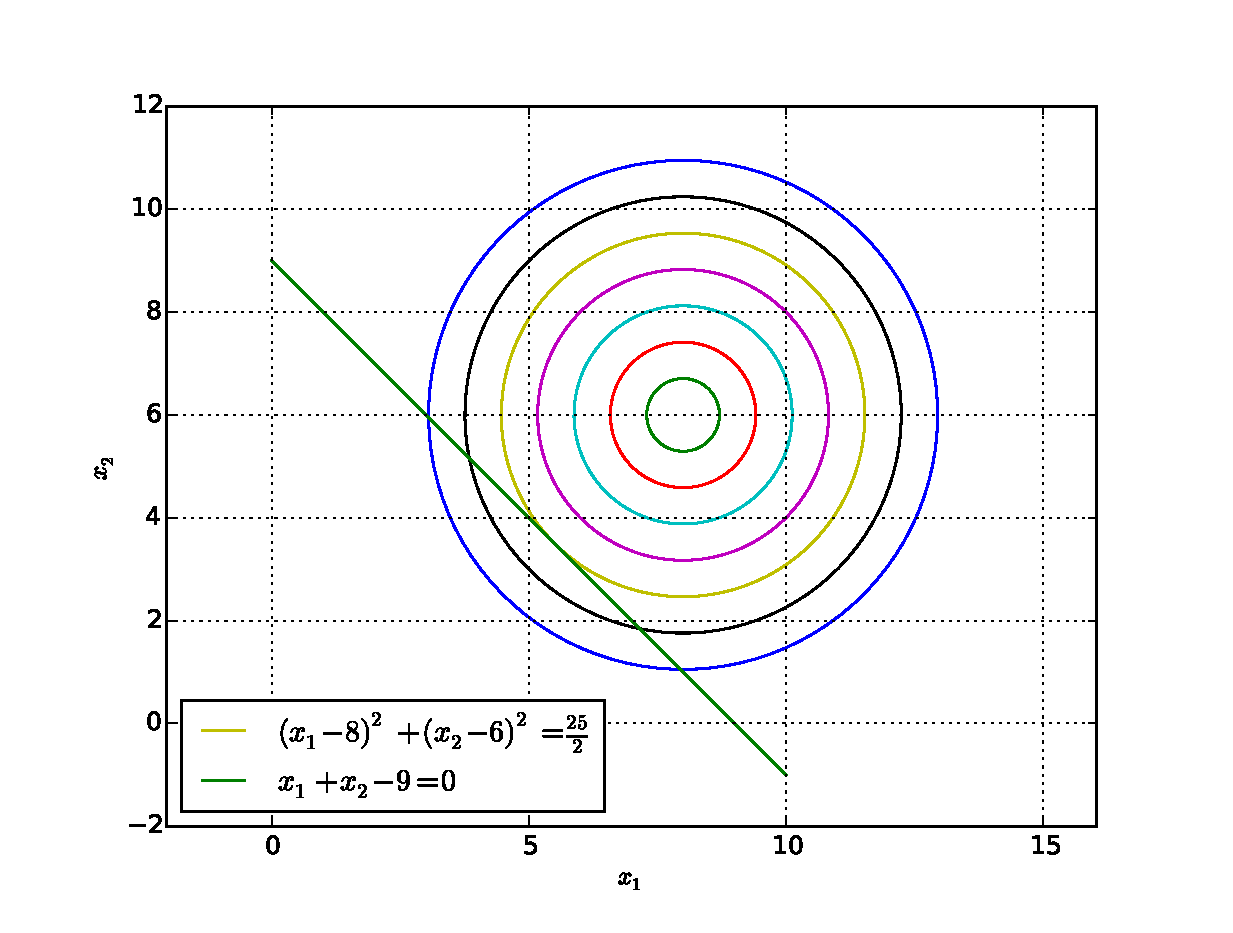
\includegraphics[width=\columnwidth]{./optimization/figs/2.1.eps}
\caption{ Finding $ \displaystyle \min_{\mbf{x}}f\brak{\mbf{x}}$}.
\label{fig.2.1}	
\end{figure}
%
\item Show that 
\begin{align}
\min r = \frac{5}{\sqrt{2}}
\end{align}
%Obtain a theoretical solution for problem \ref{convex_code} 
%%using coordinate geometry.
%
%\solution 
%From \eqref{eq2_1_line} and \eqref{eq2_1_circ}, 
%%
%\begin{align}
%r^2 & = (x_1-8)^2 + (3- x_1)^2 \\
%&= 2 x_1^2 - 22 x_1 + 73 \\
%\Rightarrow r^2 &= \frac{\brak{2x_1-11}^2 + 5^2}{2}
%\end{align}
%%
%which is minium when $x_1 = \frac{11}{2}, x_2 = \frac{7}{2}$.  The minimum value is $\frac{25}{2}$ and 
%the radius $r = \frac{5}{\sqrt{2}}$.
\item Show that 
\begin{align}
\nabla g(\vec{x}) = \myvec{1 \\ 1}
\end{align}
where
\begin{equation}
\nabla =  
\begin{pmatrix}
\frac{\partial}{\partial x_1} \\
\frac{\partial}{\partial x_2} 
\end{pmatrix}
\end{equation}

\item Show that 
\begin{align}
\nabla f(\vec{x}) = 2\cbrak{\vec{x}-\myvec{8 \\ 6}}
\end{align}
%
is the direction vector of the normal at $\vec{x}$.
\item From Fig. \ref{fig.2.1}, show that 
\begin{align}
\label{eq:opt_normal}
\nabla f(\vec{p}) = \lambda \nabla g(\vec{p}),
\end{align}
%
where $\vec{p}$ is the point of contact.
\item Use \eqref{eq:opt_normal} and $\vec{g(p)}=0$ from \eqref{eq2_1_line} to obtain $\vec{p}$.
\item
\label{lagrange}
	Define 
	\begin{equation}
	\label{lagrangian}
	L\brak{\mbf{x},\lambda} = f\brak{\mbf{x}} - \lambda g\brak{\mbf{x}}%, \quad \lambda > 0
	\end{equation}
and show that $\vec{p}$ can also be obtained by 
solving the equations
%
\begin{align}
\nabla L\brak{\mbf{x},\lambda} &= 0.
\label{tangent}
\end{align}
%
What is the sign of $\lambda$?  $L$ is known as the Lagrangian and the above technique is known as the Method of Lagrange Multipliers.

\solution
%From \eqref{eq2_1_line} and \eqref{eq2_1_circ}, 
%%
%\begin{align}
%L\brak{\mbf{x},\lambda} &= (x_1-8)^2 + (x_2-6)^2 - \lambda \brak{x_1 + x_2 - 9} \\
%\Rightarrow \nabla L\brak{\mbf{x},\lambda}  & = 
%\begin{pmatrix}
%2x_1  - 16 - \lambda \\
%2x_2 - 12 - \lambda \\
%x_1 + x_2 -9
%\end{pmatrix}
%\\
%&=
%\begin{pmatrix}
%2 &0 & - 1 \\
%0 &2 & - 1 \\
%1 & 1 & 0 
%\end{pmatrix}
%\begin{pmatrix}
%x_1 \\
%x_2 \\
%\lambda
%\end{pmatrix}
%= 
%\begin{pmatrix}
%16 \\
% 12 \\
%9
%\end{pmatrix}
%=
%0 
%\\
%\Rightarrow 
%\begin{pmatrix}
%x_1 \\
%x_2 \\
%\lambda
%\end{pmatrix}
%&= 
%\begin{pmatrix}
%\frac{11}{2} \\
% \frac{7}{2} \\
%-5
%\end{pmatrix}
%\end{align}
%%
%using the following python script.  Note that this method yields the same result as the previous exercises.  Thus, $\lambda$ is negative.
%	
\begin{lstlisting}
codes/optimization/2.3.py
\end{lstlisting}
\end{enumerate}

\subsection{Inequality Constraints}
\renewcommand{\theequation}{\theenumi}
\begin{enumerate}[label=\arabic*.,ref=\thesubsection.\theenumi]
\numberwithin{equation}{enumi}

%
\item
\label{ch2_constraint}
Modify the code in problem \ref{convex_code} to find a graphical solution for minimising
\begin{align}
f\brak{\mbf{x}} 
%= (x_1-8)^2 + (x_2-6)^2
\end{align}
with constraint
\begin{align}
%\label{convex-constraint}
g\brak{\mbf{x}} \geq 0
%= x_1 + x_2 - 9 
\end{align}

\solution 
This problem reduces to finding the radius of the smallest circle in the shaded area in Fig. \ref{fig.2.4} .  It is clear that this radius is 0.
%	
\begin{lstlisting}
codes/optimization/2.4.py
\end{lstlisting}

%
\begin{figure}[!ht]
\centering
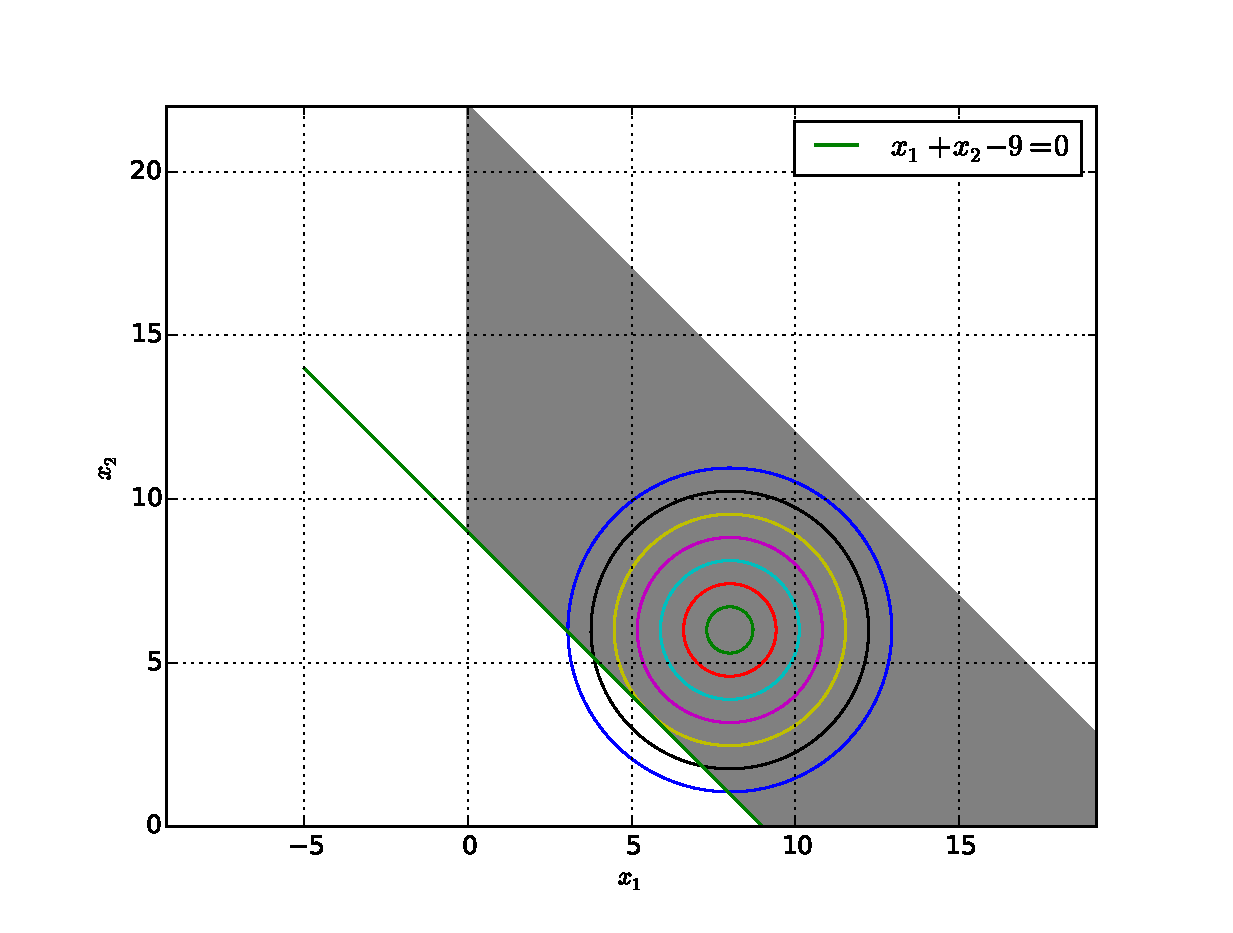
\includegraphics[width=\columnwidth]{./optimization/figs/2.4.eps}
\caption{ Smallest circle in the shaded region is a point.}
\label{fig.2.4}	
\end{figure}
%
\item
\label{ch2_lagrange_fail}
Now use the method of Lagrange multipliers to solve  problem \ref{ch2_constraint} and compare with the graphical solution.  Comment.

%
\solution Using the method of Lagrange multipliers, the solution is the same as the one obtained in  problem \ref{ch2_constraint}, which is different from the graphical solution.  This means that the Lagrange multipliers method cannot be applied blindly.
\item
Repeat problem \ref{ch2_lagrange_fail} by keeping 
 $\lambda=0$.   Comment.

\solution Keeping $\lambda = 0$ results in $\vec{x}=\myvec{ 8\\ 6}$, which is the correct solution.  The minimum value of $f\brak{\mbf{x}}$ without any constraints lies in the region $g\brak{\mbf{x}} = 0$.  In this case, $\lambda = 0$.  
%
%
\item
\label{ch2_constraint_border}
Find a graphical solution for minimising
\begin{align}
f\brak{\mbf{x}}
% = (x_1-8)^2 + (x_2-6)^2
\end{align}
with constraint
\begin{align}
%\label{convex-constraint}
g\brak{\mbf{x}} \leq 0
%= x_1 + x_2 - 9 .
\end{align}
Summarize your observations.

%
\solution In Fig. \ref{fig.2.7}, the shaded region represents the constraint.  Thus, the solution is the same as the one in problem \ref{ch2_constraint}. This implies that the method of
Lagrange multipliers can be used to solve the optimization problem with this inequality constraint as well.  Table \ref{table.2.7} summarizes the conditions for this based on the observations so far.
\begin{lstlisting}
codes/optimization/2.7.py
\end{lstlisting}

%
\begin{figure}[!ht]
\centering
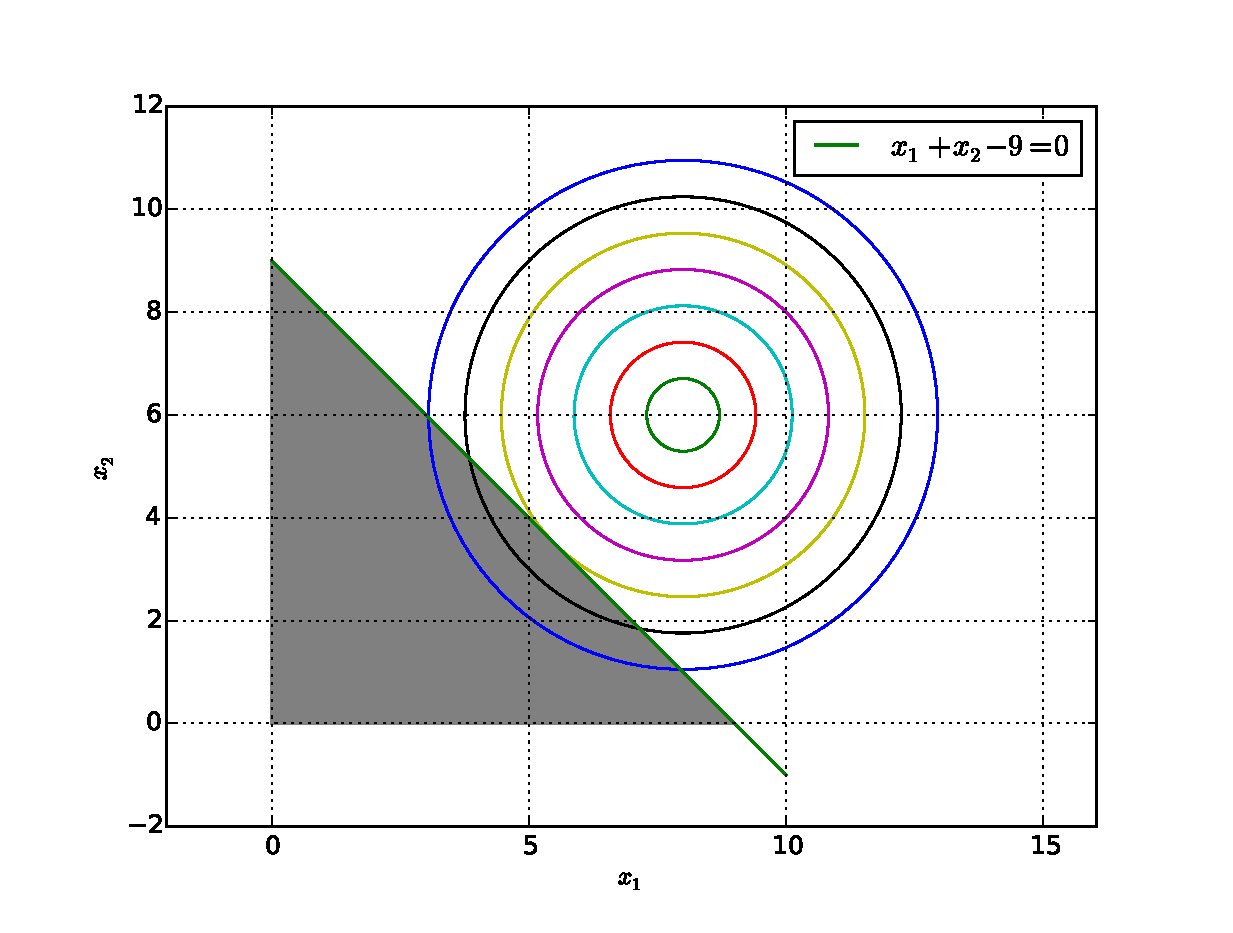
\includegraphics[width=\columnwidth]{./optimization/figs/2.7.eps}
\caption{ Finding $ \displaystyle \min_{\mbf{x}}f\brak{\mbf{x}}$.}
\label{fig.2.7}	
\end{figure}
%%%%%%%%%%%%%%%%%%%%%%%%%%%%%%%%%%%%%%%%%%%%%%%%%%%%%%%%%%%%%%%%%%%%%%
%%                                                                  %%
%%  This is the header of a LaTeX2e file exported from Gnumeric.    %%
%%                                                                  %%
%%  This file can be compiled as it stands or included in another   %%
%%  LaTeX document. The table is based on the longtable package so  %%
%%  the longtable options (headers, footers...) can be set in the   %%
%%  preamble section below (see PRAMBLE).                           %%
%%                                                                  %%
%%  To include the file in another, the following two lines must be %%
%%  in the including file:                                          %%
%%        \def\inputGnumericTable{}                                 %%
%%  at the beginning of the file and:                               %%
%%        \input{name-of-this-file.tex}                             %%
%%  where the table is to be placed. Note also that the including   %%
%%  file must use the following packages for the table to be        %%
%%  rendered correctly:                                             %%
%%    \usepackage[latin1]{inputenc}                                 %%
%%    \usepackage{color}                                            %%
%%    \usepackage{array}                                            %%
%%    \usepackage{longtable}                                        %%
%%    \usepackage{calc}                                             %%
%%    \usepackage{multirow}                                         %%
%%    \usepackage{hhline}                                           %%
%%    \usepackage{ifthen}                                           %%
%%  optionally (for landscape tables embedded in another document): %%
%%    \usepackage{lscape}                                           %%
%%                                                                  %%
%%%%%%%%%%%%%%%%%%%%%%%%%%%%%%%%%%%%%%%%%%%%%%%%%%%%%%%%%%%%%%%%%%%%%%



%%  This section checks if we are begin input into another file or  %%
%%  the file will be compiled alone. First use a macro taken from   %%
%%  the TeXbook ex 7.7 (suggestion of Han-Wen Nienhuys).            %%
\def\ifundefined#1{\expandafter\ifx\csname#1\endcsname\relax}


%%  Check for the \def token for inputed files. If it is not        %%
%%  defined, the file will be processed as a standalone and the     %%
%%  preamble will be used.                                          %%
\ifundefined{inputGnumericTable}

%%  We must be able to close or not the document at the end.        %%
	\def\gnumericTableEnd{\end{document}}


%%%%%%%%%%%%%%%%%%%%%%%%%%%%%%%%%%%%%%%%%%%%%%%%%%%%%%%%%%%%%%%%%%%%%%
%%                                                                  %%
%%  This is the PREAMBLE. Change these values to get the right      %%
%%  paper size and other niceties.                                  %%
%%                                                                  %%
%%%%%%%%%%%%%%%%%%%%%%%%%%%%%%%%%%%%%%%%%%%%%%%%%%%%%%%%%%%%%%%%%%%%%%

	\documentclass[12pt%
			  %,landscape%
                    ]{report}
       \usepackage[latin1]{inputenc}
       \usepackage{fullpage}
       \usepackage{color}
       \usepackage{array}
       \usepackage{longtable}
       \usepackage{calc}
       \usepackage{multirow}
       \usepackage{hhline}
       \usepackage{ifthen}

	\begin{document}


%%  End of the preamble for the standalone. The next section is for %%
%%  documents which are included into other LaTeX2e files.          %%
\else

%%  We are not a stand alone document. For a regular table, we will %%
%%  have no preamble and only define the closing to mean nothing.   %%
    \def\gnumericTableEnd{}

%%  If we want landscape mode in an embedded document, comment out  %%
%%  the line above and uncomment the two below. The table will      %%
%%  begin on a new page and run in landscape mode.                  %%
%       \def\gnumericTableEnd{\end{landscape}}
%       \begin{landscape}


%%  End of the else clause for this file being \input.              %%
\fi

%%%%%%%%%%%%%%%%%%%%%%%%%%%%%%%%%%%%%%%%%%%%%%%%%%%%%%%%%%%%%%%%%%%%%%
%%                                                                  %%
%%  The rest is the gnumeric table, except for the closing          %%
%%  statement. Changes below will alter the table's appearance.     %%
%%                                                                  %%
%%%%%%%%%%%%%%%%%%%%%%%%%%%%%%%%%%%%%%%%%%%%%%%%%%%%%%%%%%%%%%%%%%%%%%

\providecommand{\gnumericmathit}[1]{#1} 
%%  Uncomment the next line if you would like your numbers to be in %%
%%  italics if they are italizised in the gnumeric table.           %%
%\renewcommand{\gnumericmathit}[1]{\mathit{#1}}
\providecommand{\gnumericPB}[1]%
{\let\gnumericTemp=\\#1\let\\=\gnumericTemp\hspace{0pt}}
 \ifundefined{gnumericTableWidthDefined}
        \newlength{\gnumericTableWidth}
        \newlength{\gnumericTableWidthComplete}
        \newlength{\gnumericMultiRowLength}
        \global\def\gnumericTableWidthDefined{}
 \fi
%% The following setting protects this code from babel shorthands.  %%
 \ifthenelse{\isundefined{\languageshorthands}}{}{\languageshorthands{english}}
%%  The default table format retains the relative column widths of  %%
%%  gnumeric. They can easily be changed to c, r or l. In that case %%
%%  you may want to comment out the next line and uncomment the one %%
%%  thereafter                                                      %%
\providecommand\gnumbox{\makebox[0pt]}
%%\providecommand\gnumbox[1][]{\makebox}

%% to adjust positions in multirow situations                       %%
\setlength{\bigstrutjot}{\jot}
\setlength{\extrarowheight}{\doublerulesep}

%%  The \setlongtables command keeps column widths the same across  %%
%%  pages. Simply comment out next line for varying column widths.  %%
\setlongtables

\setlength\gnumericTableWidth{%
	53pt+%
	58pt+%
	55pt+%
0pt}
\def\gumericNumCols{3}
\setlength\gnumericTableWidthComplete{\gnumericTableWidth+%
         \tabcolsep*\gumericNumCols*2+\arrayrulewidth*\gumericNumCols}
\ifthenelse{\lengthtest{\gnumericTableWidthComplete > \linewidth}}%
         {\def\gnumericScale{\ratio{\linewidth-%
                        \tabcolsep*\gumericNumCols*2-%
                        \arrayrulewidth*\gumericNumCols}%
{\gnumericTableWidth}}}%
{\def\gnumericScale{1}}

%%%%%%%%%%%%%%%%%%%%%%%%%%%%%%%%%%%%%%%%%%%%%%%%%%%%%%%%%%%%%%%%%%%%%%
%%                                                                  %%
%% The following are the widths of the various columns. We are      %%
%% defining them here because then they are easier to change.       %%
%% Depending on the cell formats we may use them more than once.    %%
%%                                                                  %%
%%%%%%%%%%%%%%%%%%%%%%%%%%%%%%%%%%%%%%%%%%%%%%%%%%%%%%%%%%%%%%%%%%%%%%

\ifthenelse{\isundefined{\gnumericColA}}{\newlength{\gnumericColA}}{}\settowidth{\gnumericColA}{\begin{tabular}{@{}p{53pt*\gnumericScale}@{}}x\end{tabular}}
\ifthenelse{\isundefined{\gnumericColB}}{\newlength{\gnumericColB}}{}\settowidth{\gnumericColB}{\begin{tabular}{@{}p{58pt*\gnumericScale}@{}}x\end{tabular}}
\ifthenelse{\isundefined{\gnumericColC}}{\newlength{\gnumericColC}}{}\settowidth{\gnumericColC}{\begin{tabular}{@{}p{55pt*\gnumericScale}@{}}x\end{tabular}}

\begin{table}[!h]
	\caption{Summary of conditions.} 
	\centering
\begin{tabular}[c]{%
	b{\gnumericColA}%
	b{\gnumericColB}%
	b{\gnumericColC}%
	}

%%%%%%%%%%%%%%%%%%%%%%%%%%%%%%%%%%%%%%%%%%%%%%%%%%%%%%%%%%%%%%%%%%%%%%
%%  The longtable options. (Caption, headers... see Goosens, p.124) %%            \\	%
 %\hline	% Across the top of the table.
%%  The rest of these options are table rows which are placed on    %%
%%  the first, last or every page. Use \multicolumn if you want.    %%

%%  Header for the first page.                                      %%
%	\multicolumn{3}{c}{The First Header} \\ \hline 
%	\multicolumn{1}{c}{colTag}	%Column 1
%	&\multicolumn{1}{c}{colTag}	%Column 2
%	&\multicolumn{1}{c}{colTag}	\\ \hline %Last column
%	\endfirsthead

%%  The running header definition.                                  %%
%	\hline
%	\multicolumn{3}{l}{\ldots\small\slshape continued} \\ \hline
%	\multicolumn{1}{c}{colTag}	%Column 1
%	&\multicolumn{1}{c}{colTag}	%Column 2
%	&\multicolumn{1}{c}{colTag}	\\ \hline %Last column
%	\endhead

%%  The running footer definition.                                  %%
%	\hline
%	\multicolumn{3}{r}{\small\slshape continued\ldots} \\
%	\endfoot

%%  The ending footer definition.                                   %%
%	\multicolumn{3}{c}{That's all folks} \\ \hline 
%	\endlastfoot
%%%%%%%%%%%%%%%%%%%%%%%%%%%%%%%%%%%%%%%%%%%%%%%%%%%%%%%%%%%%%%%%%%%%%%

\hhline{|-|-|-}
	 \multicolumn{1}{|p{\gnumericColA}|}%
	{\gnumericPB{\centering}\textbf{Cost}}
	&\multicolumn{1}{p{\gnumericColB}|}%
	{\gnumericPB{\centering}\textbf{Constraint}}
	&\multicolumn{1}{p{\gnumericColC}|}%
	{\gnumericPB{\centering}\textbf{$\lambda$}}
\\
\hhline{|---|}
	 \multicolumn{1}{|p{\gnumericColA}|}%
	{\setlength{\gnumericMultiRowLength}{0pt}%
	 \addtolength{\gnumericMultiRowLength}{\gnumericColA}%
	 \multirow{3}[1]{\gnumericMultiRowLength}{\parbox{\gnumericMultiRowLength}{%
	 \gnumericPB{\centering}$f\brak{\mbf{x}}$}}}
	&\multicolumn{1}{p{\gnumericColB}|}%
	{\gnumericPB{\centering}$g\brak{\mbf{x}} = 0$}
	&\multicolumn{1}{p{\gnumericColC}|}%
	{\gnumericPB{\centering} $<$ 0}
\\
\hhline{~|--|}
	 \multicolumn{1}{|p{\gnumericColA}|}%
	{}
	&\multicolumn{1}{p{\gnumericColB}|}%
	{\gnumericPB{\centering}$g\brak{\mbf{x}} \geq 0 $}
	&\multicolumn{1}{p{\gnumericColC}|}%
	{\gnumericPB{\centering}0}
\\
\hhline{~|--|}
	 \multicolumn{1}{|p{\gnumericColA}|}%
	{}
	&\multicolumn{1}{p{\gnumericColB}|}%
	{\gnumericPB{\centering}$g\brak{\mbf{x}}\leq 0 $}
	&\multicolumn{1}{p{\gnumericColC}|}%
	{\gnumericPB{\centering} $<$ 0}
\\
\hhline{|-|-|-|}
\end{tabular}
\label{table.2.7}
\end{table}

\ifthenelse{\isundefined{\languageshorthands}}{}{\languageshorthands{\languagename}}
\gnumericTableEnd

%
\item
\label{ch2_prob_upper}
Find a graphical solution for 	 
	 \begin{align}
	 \label{ch2_second_min}
	\min_{\mbf{x}} f\brak{\mbf{x}} = \norm{\vec{x}-\myvec{8\\6}}^2
	 \end{align}
	 with constraint
	 \begin{align}
	 \label{ch2_second_const}
	 g\brak{\mbf{x}} = \myvec{1 & 1}\vec{x} - 18 = 0
	 \end{align}
	 
%
\solution
%	
\begin{lstlisting}
codes/optimization/2.8.py
\end{lstlisting}

%
\begin{figure}[!ht]
\centering
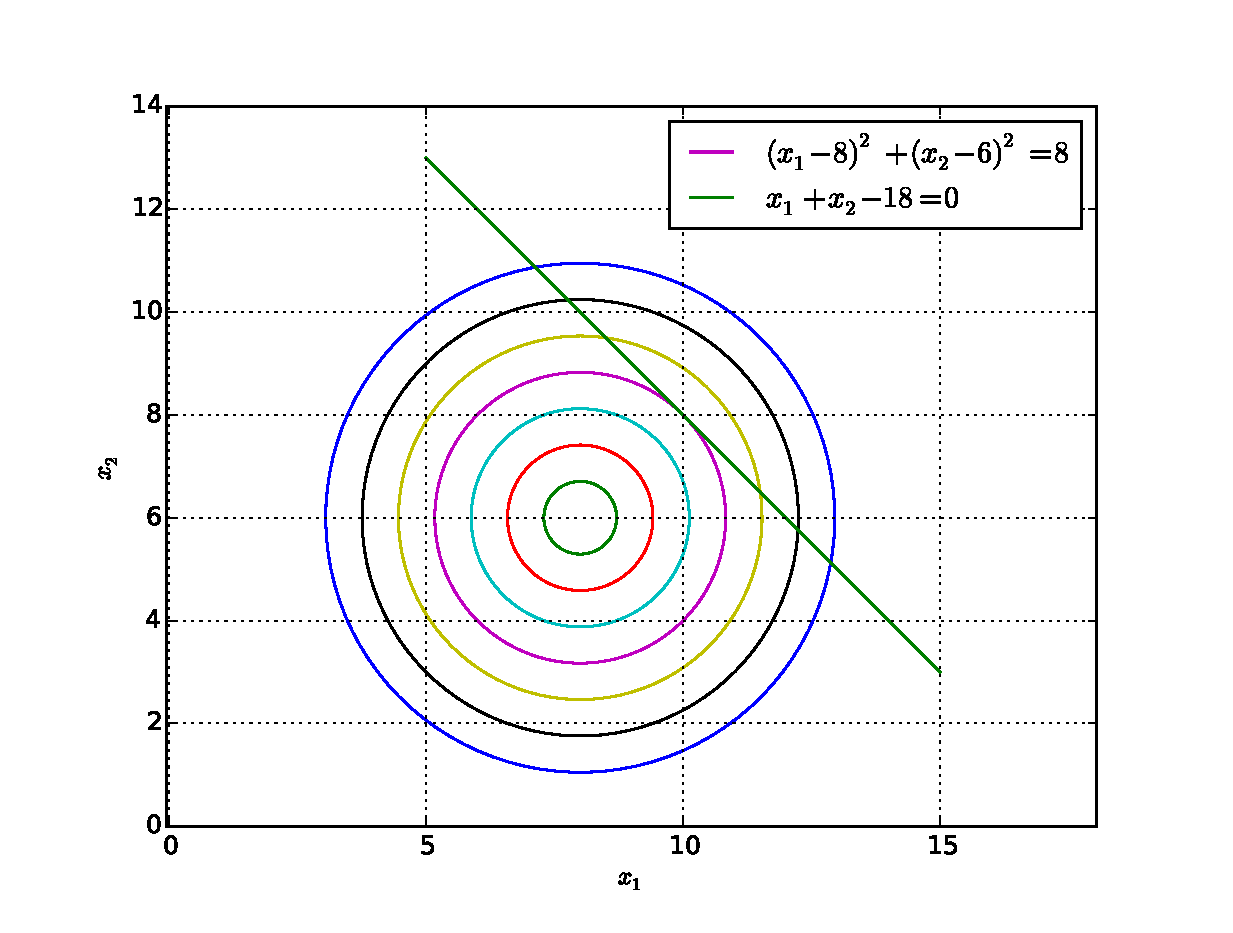
\includegraphics[width=\columnwidth]{./optimization/figs/2.8.eps}
\caption{ Finding $ \displaystyle \min_{\mbf{x}}f\brak{\mbf{x}}$.}
\label{fig.2.8}	
\end{figure}
%
\item
Repeat problem \ref{ch2_prob_upper} using the method of Lagrange mutipliers.  What is the sign of $\lambda$?

%
\solution
%From \eqref{ch2_second_min} and \eqref{ch2_second_const}, 
%%
%\begin{align}
%L\brak{\mbf{x},\lambda} &= (x_1-8)^2 + (x_2-6)^2 - \lambda \brak{x_1 + x_2 - 18} \\
%\Rightarrow \nabla L\brak{\mbf{x},\lambda}  & = 
%\begin{pmatrix}
%2x_1  - 16 - \lambda \\
%2x_2 - 12 - \lambda \\
%x_1 + x_2 -18
%\end{pmatrix}
%\\
%&=
%\begin{pmatrix}
%2 &0 & - 1 \\
%0 &2 & - 1 \\
%1 & 1 & 0 
%\end{pmatrix}
%\begin{pmatrix}
%x_1 \\
%x_2 \\
%\lambda
%\end{pmatrix}
%= 
%\begin{pmatrix}
%16 \\
% 12 \\
%18
%\end{pmatrix}
%=
%0 
%\\
%\Rightarrow 
%\begin{pmatrix}
%x_1 \\
%x_2 \\
%\lambda
%\end{pmatrix}
%&= 
%\begin{pmatrix}
%10 \\
% 8 \\
%4
%\end{pmatrix}
%\end{align}
%%
Using the following python script, $\lambda$ is positive and the minimum value of $f$ is 8.
%	
\begin{lstlisting}
codes/optimization/2.9.py
\end{lstlisting}

%
%
\item
\label{ch2_prob_upper_cond}
Solve
	 \begin{align}
%	 \label{ch2_second_min}
	\min_{\mbf{x}} f\brak{\mbf{x}} 
%= (x_1-8)^2 + (x_2-6)^2
	 \end{align}
	 with constraint
	 \begin{align}
%	 \label{ch2_second_const}
	 g\brak{\mbf{x}} 
%= x_1 + x_2 - 18 
\geq 0 
	 \end{align}
	 
%
\solution Since the unconstrained solution is outside the region $g\brak{\mbf{x}} \geq 0$, the solution is the same as the one in problem \ref{ch2_prob_upper}.
%
\item
Based on the problems so far, generalise the Lagrange multipliers method for 
%
	 \begin{align}
	 \label{ch2_lagrange_ineq}
	\min_{\mbf{x}} f\brak{\mbf{x}} , \quad 
	 g\brak{\mbf{x}}  \geq 0 
	 \end{align}
%

%
\solution
Considering $L\brak{\mbf{x},\lambda} = f\brak{\mbf{x}} - \lambda g\brak{\mbf{x}}$, for $g\brak{\mbf{x}} = \myvec{1 & 1}\vec{x} - 18 \geq 0$ we found $\lambda > 0 $ and for $g\brak{\mbf{x}} = \myvec{1 & 1}\vec{x} - 9 \leq 0, \lambda < 0$. A single condition can be obtained by framing the optimization problem as
%
	 \begin{align}
	 \label{ch2_lagrange_ineq_summary}
	\min_{\mbf{x}} f\brak{\mbf{x}} , \quad 
	 g\brak{\mbf{x}}  \leq 0 
	 \end{align}
%
with the Lagrangian
%
\begin{equation}
%\label{ch2_kkt_necessary}
L\brak{\mbf{x},\lambda} = f\brak{\mbf{x}} + \lambda g\brak{\mbf{x}}, %\quad  \lambda > 0,  g\brak{\mbf{x}} \leq 0.
\end{equation}
%
provided
%
\begin{equation}
\label{ch2_kkt_necessary}
\nabla L\brak{\mbf{x},\lambda} = 0 \Rightarrow \lambda > 0
\end{equation}
else, $\lambda = 0$.

%
\item
	\label{convex_sdp_eqiv}
	%
	Solve
	\begin{equation}
	\min_{\mbf{x}} \quad x_1 + x_2
	\end{equation}
	%	
	with the constraints
	\begin{equation}
	x_1^2 - x_1 + x_2^2 \leq 0
	\end{equation}
	%
where 
$
\mbf{x} = \begin{pmatrix}
x_1 \\
x_2
\end{pmatrix}
$

\solution 
%Using the method of Lagrange multipliers,
%%
%\begin{align}
%\label{ch2_sd_kkt}
%\nabla \cbrak{f(\mbf{x})  +  \mu g(\mbf{x}) }= 0 , \quad \mu \ge 0
%\end{align}
%%
%resulting in the equations
%%
%\begin{align}
%2x_1\mu -\mu + 1 &= 0 \\
%2x_2\mu + 1 &=0 \\
%x_1^2 -x_1 + x_2^2 &= 0 
%\end{align}
%%
%which can be simplified to obtain 
%%
%\begin{align}
%\brak{\frac{1-\mu}{2\mu}}^2 + \brak{\frac{1}{2\mu}}^2 + \frac{1-\mu}{2\mu} &= 0 \\
%\Rightarrow 1 + \mu^2 -2\mu + 1 + 2\mu\brak{1-\mu} &= 0 \\
%\Rightarrow \mu^2 =2, or \mu &= \pm \sqrt{2} 
%\end{align}
%%
%From \eqref{ch2_kkt_problem},  $\mu \ge 0 \Rightarrow  \mu = \sqrt{2}$. The desired solution is
%%
%\begin{equation}
%\mbf{x} = 
%\begin{pmatrix}
% \frac{\sqrt{2}-1}{2\sqrt{2}} \\
%-\frac{1}{2\sqrt{2}} 
%\end{pmatrix}
%\end{equation}
%
\\
{\em Graphical solution:} 
%The constraint can be expressed as
%%
%\begin{align}
%x_1^2 - x_1 + x_2^2 &\le 0 \\
%\Rightarrow \brak{x_1 - \frac{1}{2}}^2 + x_2^2 & \le \brak{\frac{1}{2}}^2
%\end{align}
%
%	
\begin{lstlisting}
codes/optimization/2.15.py
\end{lstlisting}

%
%
\begin{figure}[!ht]
\centering
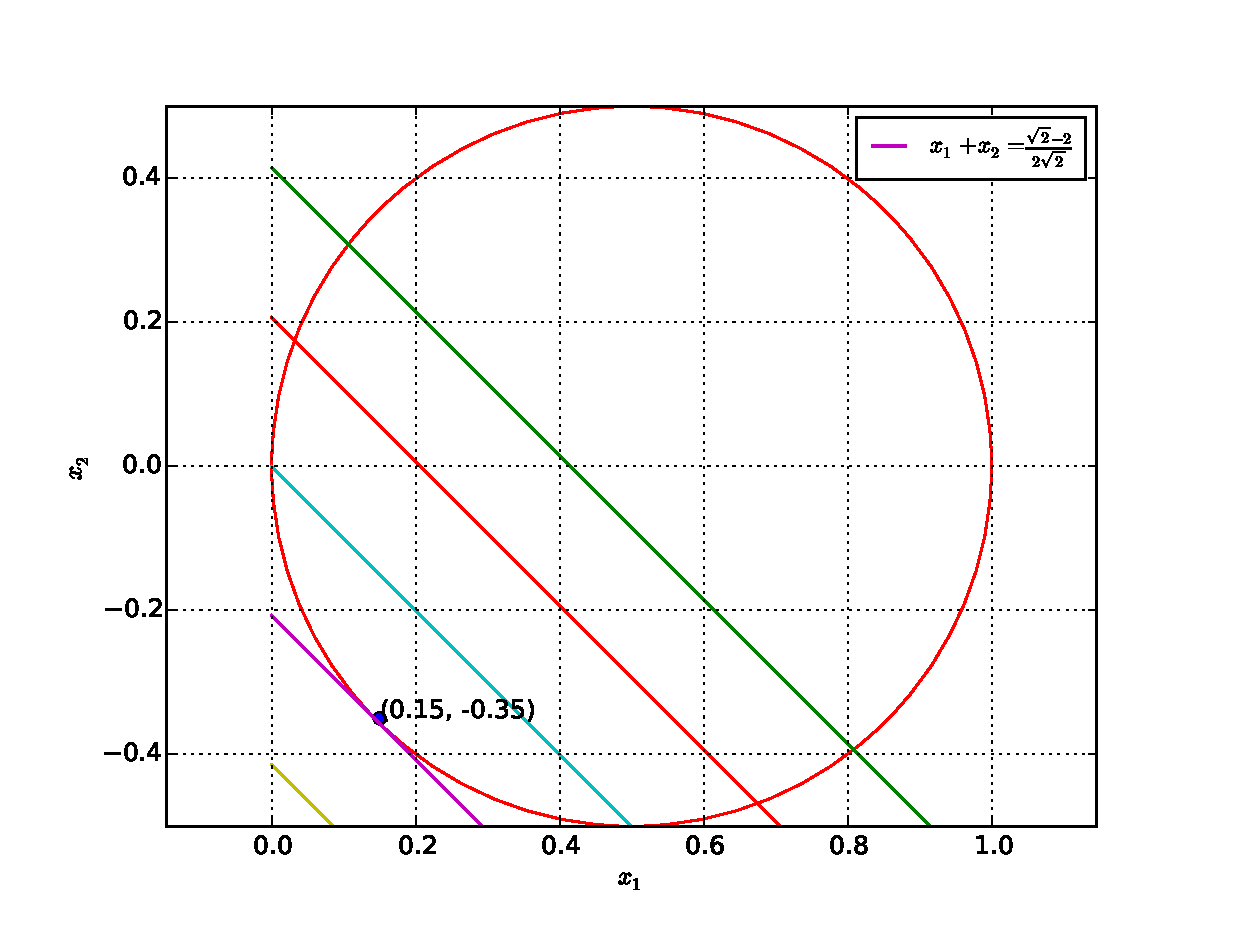
\includegraphics[width=\columnwidth]{./optimization/figs/2.15.eps}
\caption{ Optimal solution is the lower tangent to the circle}
\label{fig.2.15}	
\end{figure}
\end{enumerate}

\subsection{Solved Problems}
\renewcommand{\theequation}{\theenumi}
\begin{enumerate}[label=\arabic*.,ref=\thesubsection.\theenumi]
\numberwithin{equation}{enumi}
\item A circle passes through the points $\vec{A}=\myvec{2 \\ 3}$ and $\vec{B} = \myvec{4 \\  5}$.  If its centre $\vec{O}$ lies on the 
line
\begin{equation}
\label{eq:circle_1}
\myvec{-1 & 4}\vec{x} - 3 =0
\end{equation}
%
find its radius.
\\
\solution Let 
\begin{align}
\vec{C}=\frac{\vec{A}+\vec{B}}{2}
\implies \vec{C}=\myvec{3 \\ 4}
\label{eq:circle_1_c}
\end{align}
The direction vector of $AB$ is 
\begin{align}
\label{eq:circle_1_m}
\vec{m} = \myvec{2 \\ 3}-\myvec{4 \\  5}
= \myvec{-2 \\ -2}
\end{align}
\begin{align}
\because OC &\perp AB,
\nonumber \\
OC: \vec{m}^T\brak{\vec{x}-\vec{C}}&=0
\nonumber \\
\implies \myvec{1 & 1}\vec{x} &= 7
\label{eq:circle_1_oc}
\end{align}
%
Thus, $\vec{O}$ is the intersection of \eqref{eq:circle_1}
and \eqref{eq:circle_1_oc} and is the solution of the matrix equation
\begin{align}
 \myvec{1 & 1 \\ -1 & 4}\vec{x} &= \myvec{7 \\ 3}
\label{eq:circle_1_matrix}
\end{align}
%
From the augmented matrix,
\begin{align}
 \myvec{1 & 1 &7\\ -1 & 4 & 3}&\leftrightarrow  \myvec{1 & 1 &7\\ 0 & 1 & 2}\leftrightarrow \myvec{1 & 0 & 5\\ 0 & 1 & 2} 
\nonumber \\
\implies \vec{O} &= \myvec{5 \\ 2}
\label{eq:circle_1_o}
\end{align}
%
Thus the radius of the circle 
\begin{align}
\label{eq:circle_1_r}
OA = \norm{\vec{O}-\vec{A}} = \sqrt{10}
\end{align}
\item If a circle $C_1$, whose radius is 3, touches externally the circle 
\begin{equation}
\label{eq:circle_2_c2}
C_2: \vec{x}^T\vec{x} + \myvec{2 & -4}\vec{x} = 4
\end{equation}
%
at the point $\vec{P}=\myvec{2\\2}$, then find the length of the intercept cut by this circle $C$ on the $x$-axis.
\\
\solution From \eqref{eq:circle_2_c2}, the centre of $C_2$ is 
\begin{align}
\label{eq:circle_2_o2}
\vec{O}_2 = \myvec{-1 \\ 2}
\end{align}
%
The radius of the circle is given by 
\begin{align}
\label{eq:circle_2_r2}
r_2^2-\vec{O}_2^T\vec{O}_2 = 4 \implies r_2 = 3
\end{align}
%
%The direction vector of $O_2P$ is 
%\begin{align}
%\label{eq:circle_2_r2}
%\vec{O}_2-\vec{P} = \myvec{-3 \\ 0}
%\end{align}
%
Since the radius of $C_1$ is $r_1=r_2=3$ and $\vec{O}_1, \vec{P}, \vec{O}_2$ are collinear, 
\begin{align}
\label{eq:circle_2_o1}
\frac{\vec{O}_1+\vec{O}_2}{2} &= \vec{P}
\nonumber \\
\implies \vec{O}_1 &= 2\vec{P}-\vec{O}_2
\nonumber \\
\implies \vec{O}_1 &= \myvec{5 \\ 2}
\end{align}
%
The intercepts of $C_1$ on the $x-$axis can be expressed as 
\begin{align}
\label{eq:circle_2_x}
\vec{x}=\lambda\vec{m}
\end{align}
%
where
\begin{align}
\label{eq:circle_2_m}
\vec{m}=\myvec{1 \\ 0}
\end{align}
Susbtituting in the equation for $C_1$,
\begin{align}
\norm{\lambda\vec{m}-\vec{O}_1}^2&=r_1^2
\end{align}
which can be expressed as
\begin{align}
\lambda^2\norm{\vec{m}}^2-2\lambda\vec{m}^T\vec{O}_1+ \norm{\vec{O}_1}^2-r_1^2&=0
\nonumber \\
\implies \lambda^2-10\lambda+ 20&=0
\end{align}
resulting in
\begin{align}
\lambda&=5\pm\sqrt{5}
\label{eq:circle_2_lam}
\end{align}
%
after substituting from \eqref{eq:circle_2_m} and \eqref{eq:circle_2_o1}.


\item A line drawn through the point 
\begin{equation}
\label{eq:circle_3_p}
\vec{P} = \myvec{4\\7} 
\end{equation}
cuts the circle
\begin{equation}
\label{eq:circle_3}
C: \vec{x}^T\vec{x}  = 9
\end{equation}
at the points $\vec{A}$ and $\vec{B}$. Find $PA.PB$. Draw $PAB$ for any two points $\vec{A},\vec{B}$ on the circle.
\\
\solution Since the points $\vec{P},\vec{A},\vec{B}$ are collinear, the line $PAB$ can be expressed as
\begin{align}
L: \vec{x} = \vec{P} + \lambda \vec{m}
\label{eq:circle_3_pab}
\end{align}
%
for $\norm{\vec{m}} = 1$. The intersection of $L$ and $C$  yields
\begin{align}
\brak{\vec{P}+ \lambda \vec{m}}^T
% }
\brak{\vec{P} + \lambda \vec{m}} &= 9
\nonumber \\
\implies \lambda^2 + 2\lambda \vec{m}^T\vec{P} + \norm{\vec{P}}^2-9 &= 0
\label{eq:circle_3_quad}
\end{align}
%
The product of the roots in \eqref{eq:circle_3_quad} is 
\begin{align}
\label{eq:circle_3_prod}
PA.PB =\norm{\vec{P}}^2-9 = 56
\end{align}
%
\item Find the equation of the circle $C_2$, which is the mirror image of the circle
\begin{equation}
C_1: 
\vec{x}^T\vec{x} -\myvec{2 & 0 }\vec{x} = 0
\label{eq:circle_4}
\end{equation}
in the line
\begin{equation}
L: \myvec{1 & 1}\vec{x} = 3.
\label{eq:circle_4_line}
\end{equation}
\solution From  \eqref{eq:circle_4}, circle $C_1$ has centre at 
\begin{align}
\label{eq:circle_4_o1}
\vec{O}_1 = \myvec{1 \\ 0 }
\end{align}
%
and radius 
\begin{align}
\label{eq:circle_4_r1}
r_1 = \vec{O}_1^T\vec{O}_1 = 1
\end{align}
%
The centre of $C_2$ is the reflection of $\vec{O}_1$ about $L$ and is obtained as 
\begin{align}
\label{eq:circle_4_o2}
\frac{\vec{O}_2}{2} = \frac{\vec{m}\vec{m}^T-\vec{n}\vec{n}^T}{\vec{m}^T\vec{m}+\vec{n}^T\vec{n}}\vec{O}_1 + c 
\frac{\vec{n}}{\norm{\vec{n}}^2}
\end{align}
%
where the relevant parameters are obtained from \eqref{eq:circle_4_line} as
\begin{align}
\vec{n} =  \myvec{1 & 1}, \vec{m} =  \myvec{1 & -1}, c = 3.
\end{align}
%
Substituting the above in \eqref{eq:circle_4_o2},
\begin{align}
\label{eq:circle_4_o2_final}
\frac{\vec{O}_2}{2} &= \frac{\myvec{1 & 1 \\ 1 & 1}-\myvec{1 & -1 \\ -1 & 1}}{4}\vec{O}_1 + c 
\frac{\vec{n}}{2}
\nonumber \\
\implies \vec{O}_2 &= \myvec{3 \\ 4}
\end{align}
%
Thus
\begin{align}
C_2: \norm{\vec{x}- \myvec{3 \\ 4}} = 1
\label{eq:circle_4_c2}
\end{align}

%\item Find the locus of the centres of those circles which touch the circle
%\begin{equation}
%C:
%\vec{x}^T\vec{x} -8\myvec{1 & 1 }\vec{x} = 4
%\label{eq:circle_5}
%\end{equation}
%and also touch the $x$-axis.
%\\
%\solution $C$ has centre at 
%\begin{align}
%\vec{O} = 4 \myvec{1 \\ 1 } 
%\label{eq:circle_5_o}
%\end{align}
%%
%Let $\vec{y}$ be the centre of the desired circle. 
%If $\vec{p}$ be the point of contact, since $\vec{y},\vec{p},\vec{O}$ are collinear, 
%\begin{align}
%\vec{p} = \frac{\vec{y}+\vec{O}}{2}
%\label{eq:circle_5_p}
%\end{align}
%
%
%Since the circle touches the $x-axis$, the x-axis is its tangent.
\item One of the diameters of the circle, given by 
\begin{equation}
C: \vec{x}^T\vec{x} +2\myvec{-2 & 3 }\vec{x} = 12
\label{eq:circle_6_c}
\end{equation}
is a chord of a circle $S$, whose centre is at 
\begin{equation}
\vec{O}_2=\myvec{-3\\ 2}.
\label{eq:circle_6_o2}
\end{equation}
Find the radius of $S$.
\\
\solution From \eqref{eq:circle_6_c}, the centre of $C$ is 
\begin{align}
\vec{O}_1 = \myvec{2\\ -3} 
\label{eq:circle_6_o1}
\end{align}
%
and the radius is 
\begin{align}
r_1 = \sqrt{\vec{O}_1^T\vec{O}_1-12} = 5
\label{eq:circle_6_r1}
\end{align}
%
From \eqref{eq:circle_6_o1} and \eqref{eq:circle_6_o2},
\begin{align}
O_1O_2 = \norm{\vec{O}_1-\vec{O}_2}=5\sqrt{2}
\nonumber \\
\label{eq:circle_6_o1o2}
\implies r_2 = \sqrt{O_1O_2^2-r_1^2} = 5
\end{align}

\item A circle $C$ passes through 
\begin{equation} 
\vec{P}=\myvec{-2\\ 4} 
\label{eq:circle_7_p}
\end{equation} 
and touches the $y$-axis at 
\begin{equation} 
\vec{Q}=\myvec{0\\ 2}. 
\label{eq:circle_7_q}
\end{equation}
Which one of the  following equations can represent a diameter of this circle?
\begin{enumerate}[label=(\roman*)]
\begin{multicols}{2}
\setlength\itemsep{1em}
\item $\myvec{4 & 5}\vec{x} = 6 $
\item $\myvec{2 & -3}\vec{x} +10 = 0 $
\item $\myvec{3 & 4}\vec{x} = 3 $
\item $\myvec{5 & 2}\vec{x} +4= 0 $
\end{multicols}
\end{enumerate}

\solution Let $\vec{O}$ be the centre of $C$. Then the equation of the normal, OQ is
\begin{align}
%\vec{x}^T\vec{x}-2\vec{O}^T\vec{x} +F = 0
\myvec{0 & 1}\brak{\vec{O}-\vec{Q}} &= 0
\nonumber \\ 
\implies \myvec{0 & 1}\vec{O} = 2
\label{eq:circle_7_o1}
\end{align}
%
Also, 
%Substituting \eqref{eq:circle_7_p} in \eqref{eq:circle_7_c}, 
\begin{align}
\norm{\vec{O}-\vec{P}}^2&=\norm{\vec{O}-\vec{Q}}^2 
\nonumber \\
\implies 2\brak{\vec{P}-\vec{Q}}^T\vec{O} &= \norm{\vec{P}}^2-\norm{\vec{Q}}^2 
\nonumber \\
\text{or, } \myvec{1 & -1}\vec{O} &= -4
\label{eq:circle_7_o2}
\end{align}
%
\eqref{eq:circle_7_o1} and \eqref{eq:circle_7_o2} result in the matrix equation
\begin{align}
\myvec{1 & -1 \\ 0 & 1}\vec{O} = \myvec{-4\\2}
\label{eq:circle_7_matrix}
\end{align}
yielding the augmented matrix
\begin{align}
\myvec{1 & -1 & -4\\ 0 & 1 & 2} \leftrightarrow \myvec{1 & 0 & -2\\ 0 & 1 & 2}\implies \vec{O} = \myvec{-2 \\2}
\label{eq:circle_7_o}
\end{align}
Hence, option ii)  is correct.
\item Find the equation of the tangent to the circle, at the point
\begin{equation}
\vec{P}=\myvec{1\\ -1},
\end{equation}
whose centre $\vec{O}$ is the point of intersection of the straight lines
\begin{align} 
\label{eq:circle_8_o1}
\myvec{2 & 1}\vec{x} &= 3
\\
\myvec{1 & -1}\vec{x} &= 1
\label{eq:circle_8_o2}
\end{align} 
\solution From \eqref{eq:circle_8_o1} and \eqref{eq:circle_8_o2}, we obtain the matrix equation
\begin{align} 
\myvec{2 & 1\\1 & -1}\vec{O} &= \myvec{3 \\ 1}
\end{align} 
yielding the augmented matrix
\begin{align} 
\myvec{1 & -1 & 1\\2 & 1 & 3}&\leftrightarrow\myvec{1 & -1 & 1\\0 & 3 & 1}
\nonumber \\
\leftrightarrow\myvec{3 & 0 & 4\\0 & 3 & 1}&\implies \vec{O} = \frac{1}{3}\myvec{4 \\ 1}
\end{align} 
%
Thus, the equation of the desired tangent is 
\begin{align} 
\brak{\vec{O}-\vec{P}}^T\brak{\vec{x}-\vec{P}} &= 0
\nonumber \\
\implies
\myvec{1 & 4}\vec{x}=-3
\end{align} 
%\end{enumerate}
%\section{Vector Algebra}
%\begin{enumerate}[label=\thesection.\arabic*
%,ref=\thesection.\theenumi]

\item The line 
\begin{align}
\Gamma: \vec{x} = \myvec{0 \\ 1} + \lambda \myvec{1 \\ m}
\label{eq:coord_line}
\end{align}
intersects the circle
\begin{align}
\Omega: \norm{\vec{x}-\myvec{3 \\ -2}} = 5
\label{eq:coord_circ}
\end{align}
at points $\vec{P}$ and $\vec{Q}$ respectively. The mid point of $PQ$ is 
$\vec{R}$ such that
\begin{align}
\myvec{1 & 0}\vec{R} = -\frac{3}{5}
\label{eq:coord_mid}
\end{align}
%
Find $m$.
\\
\solution Let 
\begin{align}
\vec{c} = \myvec{0 \\ 1}, \vec{O} = \myvec{3 \\ -2} \text{ and } \vec{m} = 
\myvec{1 \\ m}
\label{eq:coord_defs}
\end{align}
%
The intersection of  \eqref{eq:coord_line} and \eqref{eq:coord_circ} is 
\begin{align}
\norm{\vec{c}+\lambda\vec{m} -\vec{O}}^2 = 25
\end{align}
\begin{multline}
\label{eq:coord_quad}
\implies \lambda^2 \norm{\vec{m}}^2+ 2\lambda\vec{m}^{T}\brak{\vec{c} 
-\vec{O}}
\\
+\norm{\vec{c} -\vec{O}}^2-25 = 0
\end{multline}
%
Since $\vec{P}, \vec{Q}$ lie on $\Gamma$,
\begin{align}
\vec{P} &= \vec{c}+\lambda_1\vec{m} 
\\
\vec{Q} &= \vec{c}+\lambda_2\vec{m} 
\\
\implies \frac{\vec{P}+\vec{Q}}{2} &= \vec{c} + 
\frac{\lambda_1+\lambda_2}{2}\vec{m} 
\\
\implies \myvec{1 & 0}\frac{\vec{P}+\vec{Q}}{2} &= \myvec{1 & 0}\vec{c}
\nonumber \\
& \,+ \frac{\lambda_1+\lambda_2}{2}\myvec{1 & 0}\vec{m} 
\\
&= \myvec{1 & 0}\vec{c} -
\frac{\vec{m}^{T}\brak{\vec{c} -\vec{O}}}{\norm{\vec{m}}^2}
\end{align}
using the sum of roots in \eqref{eq:coord_quad}.  From 
\eqref{eq:coord_mid} and \eqref{eq:coord_defs},
\begin{align}
-\myvec{1 & m}\myvec{-3\\3}= -\frac{3}{5}\brak{1+m^2}
\\
\implies m^2 -5m + 6 = 0
\\
\implies m = 2 \text{ or } 3
\end{align}
From \eqref{eq:coord_quad}, 
\begin{multline}
\lambda = \frac{-\vec{m}^{T}\brak{\vec{c} -\vec{O}}}{{\norm{\vec{m}}^2}}
\\
\pm \frac{\sqrt{\brak{\vec{m}^{T}\brak{\vec{c} -\vec{O}}}^2
-\norm{\vec{c} -\vec{O}}^2+25}}{\norm{\vec{m}}^2}
\end{multline}
Fig. \ref{fig:2019_3} summarizes the solution for $m = 2$.

%\renewcommand\thefigure{\theenumi}

\begin{figure}
\centering
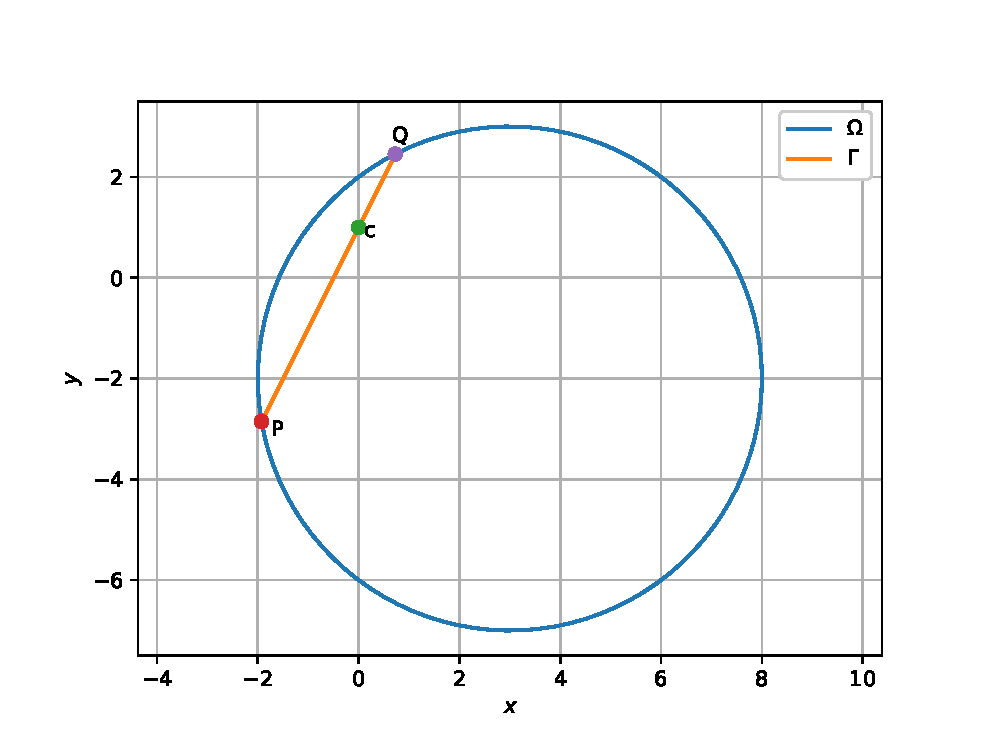
\includegraphics[width=\columnwidth]{./circle/figs/2019_3.eps}
\caption{}
\label{fig:2019_3}
\end{figure}
\end{enumerate}
%\section{Linear Algebra: Reflection}
%\begin{enumerate}[label=\thesection.\arabic*
%,ref=\thesection.\theenumi]
%\item Let $\vec{B}$ be the reflection of $\vec{A} = \myvec{2 \\ 3}$ with respect to the line 
%\begin{align}
%L: \myvec{8 & -6}\vec{x} = 23
%\end{align}
%%
%Show that $\vec{B} = \myvec{6 \\ 0}$.
%%\\
%%\solution The normal vector of $L$ is 
%%\begin{align}
%%\vec{n} &= \myvec{8 & -6}
%%\\
%%\implies \vec{m} &= \myvec{6 & 8}
%%\end{align}
%%%
%%Letting $c = 23$, 
%%\begin{align}
%%\frac{\vec{B}}{2}= \frac{\vec{m}\vec{m}^T-\vec{n}\vec{n}^T}{\vec{m}^T\vec{m}+\vec{n}^T\vec{n}}\vec{A}+c\frac{\vec{n}}{\vec{\norm{n}}}
%%\end{align}
%
%\item Find the equation of $AB$.
%\\
%\solution The normal vector of $L$ is
%\begin{align}
%\vec{n} = \myvec{6 \\ 8}
%\end{align}
%%
%Thus, the equation of $AB$  is
%\begin{align}
%AB: \vec{n}^T\brak{\vec{x}-\vec{A}} &= 0
%\\
%\implies \myvec{6 & 8}\vec{x} & = 36 
%\end{align}
%
%\item Let $\Gamma_A$ and $\Gamma_B$ be circles of radii $r_1 = 2, r_2 = 1$ with centres at $\vec{A}$ and $\vec{B}$ respectively. Let $T$ be the common tangent to both the circles such that they are on the same side of $T$. 
%\item Find the point $\vec{C}$ where $AB$ meets $T$.
%\\
%\solution Let $\vec{D}, \vec{E}$ be the points of contact for $T$ with $\Gamma_A$ and 4$\Gamma_B$ respectively. It is obvious that $\triangle ADC \sim \triangle BEC$. Hence, 
%\begin{align}
%AB &= BC 
%\\
%\implies \vec{C} &= 2\vec{B}-A = \myvec{10 \\ -3}
%\end{align}
%\item Find $AC$.
%\\
%\solution 
%\begin{align}
%AC = \norm{\vec{A}-\vec{C}} = 10
%\end{align}
%-\item Find  $\vec{D}$ and  $\vec{E}$.
%\end{enumerate}
%\section{Linear Algebra: Coordinate Geometry}
%%
%\begin{enumerate}[label=\thesection.\arabic*
%,ref=\thesection.\theenumi]
%\item Find the points $\vec{X},\vec{Y}$ where 
%\begin{align}
%\label{eq:2019_qp2_17_c1c2}
%C_1: \norm{\vec{x}} &= 3
%\\
%C_2: \norm{\vec{x}-\myvec{3 \\4}} &= 4
%\end{align}
%%
%intersect. 
%\item Find the centre $\vec{O}_3$ and radius $r$ of $C_3$ such that
%\begin{enumerate}
%\item $\vec{O}_1, \vec{O}_2, \vec{O}_3$ are collinear.
%\item $C_1, C_2$ lie inside $C_3$ and 
%\item $C_3$ touches $C_1$ at $\vec{M}$ and $C_2$ at $\vec{N}$.
%\end{enumerate}
%\item Find the equation of $XY$.
%\item Find $\vec{Z}, \vec{W}$ the points of intersection of $XY$ and $C_3$.
%\item A common tangent of $C_1$ and $C_3$ is also a tangent to 
%\begin{align}
%\label{eq:2019_qp2_17_c1c2}
%P: \vec{x}^T\myvec{1 & 0 \\ 0 & 0}\vec{x} - 2\alpha\myvec{0 & 1}\vec{x} = 0
%\end{align}
%%
%Find $\alpha$.
%\end{enumerate}
%\section{Linear Algebra: Coordinate Geometry}
%Find the following based on the previous problem
%\begin{enumerate}[label=\thesection.\arabic*
%,ref=\thesection.\theenumi]
%%
%\item $\myvec{2 & 1}\vec{O}_3$
%\item $\frac{ZW}{XY}$
%\item $\frac{\text{ar}\brak{\triangle MZN}}{\text{ar}\brak{\triangle ZMW}}$
%\end{enumerate}


%\end{document}
 
\subsection{JEE Exercises}
\renewcommand{\theequation}{\theenumi}
\begin{enumerate}[label=\arabic*.,ref=\thesubsection.\theenumi]
\numberwithin{equation}{enumi}
\item If A and B are points in the plane such that $\frac{PA}{PB} = k\text{(constant)}$ for all $\vec{P}$ on a given circle, then the value of k cannot be equal to?
 
\item Find the points of intersection of the line 
\begin{align} 
\myvec{4 & -3}\vec{x} - 10 = 0
\end{align} 
and the circle 
\begin{align}
\vec {x}^T\vec{x} + \myvec{-2 & 4}\vec{x} - 20 = 0.
\end{align}
are...................and................

\item The lines 
\begin{align}
\myvec{3 & -4}\vec{x} + 4 = 0 \\
\myvec{6 & -8}\vec{x} - 7 = 0
\end{align} 
are tangents to the same circle. The radius of the circle is.............

\item Let 
\begin{align}
\vec{x}^T \vec{x} + \myvec{-4 & -2}\vec{x} - 11 = 0
\end{align} 
be circle. A pair of tangents $\myvec{4 & 5}$ with a pair radii from quadrilateral of area..............

\item From the origin chords are drawn to the circle 
\begin{align}
\vec{x}^T\vec{x} + \myvec{-2 & 0}\vec{x} = 0
\end{align} 
The equation of the locus of the mid-points of these chords is............

\item The equation of the line passing through the points of intersection of the circles 
\begin{align}
3(\vec{x}^T\vec{x}) + \myvec{-2 & 12}\vec{x} - 9 = 0 \\
\vec{x}^T\vec{x} + \myvec{6 & 2}\vec{x} - 15 = 0
\end{align} 
is................

\item From the point A$\myvec{0 & 3}$ on the circle 
\begin{align}
\vec{x}^T\vec{x} + \myvec{4 & 6}\vec{x} + 9 = 0
\end{align} 
a chord AB is drawn and extended to a point $\vec{M}$ such that AM = 2AB. The equation of the locus of 
$\vec{M}$ is..............

\item The area of the triangle is formed by tangents from the point $\myvec{4 & 3}$ to the circle 
\begin{align}
\vec{x}^T\vec{x} = 9
\end{align} 
and the line joining their points of contact is

\item If the circle 
\begin{align}
C_1:\vec{x}^T\vec{x} = 16
\end{align} 
intersects another circle $C_2$ of radius 5 in such a manner that common chord is of maximum length and has a slope equal to $\frac{3}{4},$ then the coordinates of the centre $C_2$ are...........

\item The area of the triangle formed by the positive x-axis and the normal and the tangent to the circle 
\begin{align}
\vec{x}^T\vec{x} = 4
\end{align} 
at (1, $\sqrt{3}$)is?

\item If a circle passes through the points of intersection of the coordinate axes with the lines 
\begin{align}
\myvec{\lambda & -1}\vec{x} + 1 = 0\\
\myvec{1 & -2}\vec{x} + 3 = 0
\end{align} 
then the value of $\lambda$ = .............. 

\item The equation of the locus of the midpoints of the circle 
\begin{align}
4(\vec{x}^T\vec{x}) + \myvec{-12 & 4}\vec{x} + 1 = 0
\end{align} 
that subtend of a angle of $\frac{2\pi}{3}$  at its centre is..............

\item The intercept on the line
\begin{align} 
\myvec{1 & -1}\vec{x} = 0
\end{align}
by the circle
\begin{align}
C1:\vec{x}^T\vec{x} + \myvec{-2 & 0}\vec{x}=0
\end{align} 
is AB. Equation of the circle with AB as a diameter is...............

\item For each natural number k, let $C_k$ denote the circle with radius k centimetres and center at origin. On the circle $C_k$, $\alpha$-particle moves k centimetres in the counter clockwise direction. After completing its motion on $C_k$ the particle moves to $C_{k+1}$ in the radial direction. The motion of the particle is continues in the manner. The particle starts at $\myvec{1 & 0}$. If the particle crosses the positive direction of the x-axis for the first time on the circle $C_n$ then n=................

\item The chords of contact of the pair of tangents drawn from each point on the line 
\begin{align}
\myvec{2 & 1}\vec{x} = 4
\end{align} 
to circle 
\begin{align}
\vec{x}^T\vec{x} = 1
\end{align} 
pass through the point?

\item  A square is inscribed in the circle  
\begin{align}
\vec{x}^T\vec{x} + \myvec{-2 & 4}\vec{x} + 3 = 0.
\end{align} 
Its sides are parallel to the coordinate axes. The one vertex of the square is
\begin{enumerate}
\item $(1 + \sqrt{2}, -2)$
\item $(1 - \sqrt{2}, -2)$
\item $(1, -2+\sqrt{2})$
\item none of these
\end{enumerate}

\item Two circles 
\begin{align}
\vec{x}^T\vec{x} = 6 and \\
\vec{x}^T\vec{x} + \myvec{-6 & 8}\vec{x} + 3 = 0
\end{align} 
are given. Then the equation of the circle through their points of intersection and the point $\myvec{1 & 1}$ is
\begin{enumerate}
\item $\vec{x}^T\vec{x} + \myvec{-6 & 0}\vec{x} + 4 = 0$
\item $\vec{x}^T\vec{x} + \myvec{-3 & 0}\vec{x} + 1 = 0$
\item $\vec{x}^T\vec{x} + \myvec{0 & -4}\vec{x} + 2 = 0$
\item none of these
\end{enumerate}

\item The centre of the circle passing through the point $\myvec{0 & 1}$ and touching the curve 
\begin{align}
y = \vec{x}^T\myvec{1 & 0 \\ 0 & 0}\vec{x}
\end{align} 
at $\myvec{2 & 4}$ is
\begin{enumerate}
\item $(\frac{-16}{5}, \frac{27}{10})$
\item $(\frac{-16}{7}, \frac{53}{10})$
\item $(\frac{-16}{5}, \frac{53}{10})$
\item none of these
\end{enumerate}
    
\item The equation of the circle passing through the point $\myvec{1 & 1}$ and the points of intersection of 
\begin{align} 
\vec{x}^T\vec{x} + \myvec{13 & -3}\vec{x} = 0 \\
2(\vec{x}^T\vec{x}) + \myvec{4 & -7}\vec{x} - 25 = 0
\end{align} 
is 
\begin{enumerate}
\item $4(\vec x^T\vec x) + \myvec{-30 & -10}\vec{x} - 25 = 0$
\item $4(\vec x^T\vec x) + \myvec{30 & -13}\vec{x} - 25 = 0$
\item $4(\vec x^T\vec x) + \myvec{-17 & -10}\vec{x} + 25 = 0$
\item none of these
\end{enumerate}

\item The locus of the mid point of a chord of the circle
\begin{align}
\vec{x}^T\vec{x} = 4
\end{align} 
which subtends a right angle at the origin is
\begin{enumerate}
\item $\myvec{1 & 1}\vec{x} = 2$
\item $\vec{x}^T\vec{x} = 1$
\item $\vec{x}^T\vec{x} = 2$
\item $\myvec{1 & 1}\vec{x} = 1$
\end{enumerate}

\item If a circle passes through the point $\myvec{a & b}$ and cuts the circle 
\begin{align}
\vec{x}^T\vec{x} = k^{2}
\end{align} 
orthogonally, then the equation of the locus of its centre is  
\begin{enumerate}
\item $\myvec{2a & 2b}\vec{x} - (a^2 + b^2 + k^2) = 0$
\item $\myvec{2a & 2b}\vec{x} - (a^2 - b^2 + k^2) = 0$
\item $\vec{x}^T\vec{x} + \myvec{-3a, -4b}\vec{x} + (a^2 + b^2 - k^2) = 0$
\item $\vec{x}^T\vec{x} + \myvec{-3a, -4b}\vec{x} + (a^2 - b^2 - k^2) = 0$
\end{enumerate}

\item If the two circles 
\begin{align}
\vec{x}^T\vec{x} + \myvec{-2 &-2}\vec{x} + 2 = r^{2} \\
\vec{x}^T\vec{x} + \myvec{-8 & 2}\vec{x} + 8 = 0
\end{align} 
intersect in two distinct points, then
\begin{enumerate}
\item $2 < r < 8$
\item $r < 2$
\item r = 2
\item $r > 2$
\end{enumerate}

\item The lines 
\begin{align}
\myvec{2 & -3}\vec{x} = 5 \\
\myvec{3 & -4}\vec{x} = 7
\end{align}
are diameters of a circle of area 154 sq.units. Then the equation of this circle is
\begin{enumerate}
\item $ \vec{x}^T\vec{x} + \myvec{2 & -2}\vec{x} = 62$
\item $ \vec{x}^T\vec{x} + \myvec{2 & -2}\vec{x} = 47$
\item $ \vec{x}^T\vec{x} + \myvec{-2 & 2}\vec{x} = 47$
\item $ \vec{x}^T\vec{x} + \myvec{-2 & 2}\vec{x} = 62$
\end{enumerate}

\item Find the centre of a circle passing through the points $\myvec{0 & 0}$, $\myvec{1 & 0}$ and touching the circle
\begin{align}
\vec{x}^T\vec{x} = 9.
\end{align}
\begin{enumerate}
\item $(\frac{3}{2}, \frac{1}{2})$
\item $(\frac{1}{2}, \frac{3}{2})$
\item $(\frac{1}{2}, \frac{1}{2})$
\item $(\frac{1}{2}, (-2)^{\frac{1}{2}})$
\end{enumerate}
     
\item The locus of the centre of a circle, which touches externally the circle 
\begin{align}
\vec{x}^T\vec{x} + \myvec{-6 & -6}\vec{x} + 14 = 0
\end{align}
and also touches the y-axis, is given by the equation:
\begin{enumerate}
\item $\vec{x}^T \myvec{1 & 0 \\ 0 & 0}\vec{x} + \myvec{-6 & 10} \vec{x} + 14 = 0$
\item $\vec{x}^T \myvec{1 & 0 \\ 0 & 0}\vec{x} + \myvec{-10 & -6}\vec{x} + 14 = 0$
\item $\vec{x}^T \myvec{1 & 0 \\ 0 & 0}\vec{x} + \myvec{-6 & -10}\vec{x} + 14 = 0$
\item $\vec{x}^T \myvec{1 & 0 \\ 0 & 0}\vec{x} + \myvec{-10 & -6} \vec{x} + 14 = 0$
\end{enumerate}

\item The circles 
\begin{align}
\vec{x}^T\vec{x} + \myvec{-10 & 0}\vec{x} + 16 = 0 \\
\vec{x}^T\vec{x} = r^{2}
\end{align}
intersect each other in two distinct points if
\begin{enumerate}
\item $r < 2$
\item $r > 8$
\item $2 < r < 8$
\item $2 \leq r \leq  8$
\end{enumerate}
 
\item The angle between a pair of tangents drawn  from a point $\vec{P}$  to the circle 
\begin{align}
\vec{x}^T\vec{x} + \myvec{4 & -6}\vec{x} + 9\sin{^{2}(\alpha)} + 13\cos{^2(\alpha)} = 0
\end{align} 
is $2\pi$. The equation of the locus of the point $\vec{P}$ is 
\begin{enumerate}
\item $\vec{x}^T\vec{x} + \myvec{4 & -6}\vec{x} + 4 = 0$
\item $\vec{x}^T\vec{x} + \myvec{4 & -6}\vec{x} - 9 = 0$
\item $\vec{x}^T\vec{x} + \myvec{4 & -6}\vec{x} - 4 = 0$
\item $\vec{x}^T\vec{x} + \myvec{4 & -6}\vec{x} + 9 = 0$  
\end{enumerate}
    
\item If two distinct chords drawn from the point (p, q) on the circle 
\begin{align}
\vec{x}^T\vec{x} = \myvec{p & q}\vec{x}
\end{align}
(where pq $\neq$ 0) are bisected by the x-axis, then 
\begin{enumerate}
\item $p^2 = q^2$
\item $p^2 = 8q^2$
\item $p^2 < 8q^2$
\item $p^2 > 8q^2$   
\end{enumerate}
    
\item The triangle PQR is inscribed in the circle 
\begin{align}
\vec{x}^T\vec{x} = 25.
\end{align} 
If $\vec{Q}$ and $\vec{R}$ have co-ordinates \myvec{3 \\ 4} and \myvec{-4 \\ 3} respectively, then 
$\angle QPR$ is equal to
\begin{enumerate}
\item $\frac{\pi}{2}$
\item $\frac{\pi}{3}$
\item $\frac{\pi}{4}$
\item $\frac{\pi}{6}$
\end{enumerate}
    
\item If the circles 
\begin{align}
\vec{x}^T\vec{x}+\myvec{2 & 2k}\vec{x}+6=0 \\
\vec{x}^T\vec{x}+\myvec{0&2k}\vec{x}+k=2
\end{align} 
intersect orthogonally, then find k.

\item Let AB be chord of the circle 
\begin{align}
\vec{x}^T\vec{x}=r^2
\end{align} 
subtending a right angle at at the centre. Then the locus of the centroid of the triangle PAB as $\vec{P}$ moves on the circle is
\begin{enumerate}
\item a parabola
\item a circle
\item a ellipse
\item a pair of straight lines 
\end{enumerate}

\item Let PQ and RS be tangents at the extremities of the diameter PR of a circle of radius r. If PS and RQ intersect at a point on the circumference of the circle, then 2r equals
\begin{enumerate}
\item $\sqrt{PQ.RS}$
\item $\frac{(PQ+RS)}{2}$
\item $\frac{2PQ.RS}{(PQ+RS)}$
\item $\frac{\sqrt{(PQ^2+RS^2)}}{2}$ 
\end{enumerate}
    
\item If the tangent at the point $\vec{P}$ on the circle 
\begin{align}
\vec{x}^T\vec{x}+\myvec{6&6}\vec{x}-2=0
\end{align}
meets a straight line 
\begin{align}
\myvec{5&-2}\vec{x}+6=0
\end{align}
at a point $\vec{Q}$ on the y-axis then the length of PQ is
\begin{enumerate}
\item 4
\item 2$\sqrt{5}$
\item 5
\item 3$\sqrt{5}$ 
\end{enumerate}
    
\item Find the centre of the circle inscribed in square formed by the lines 
\begin{align}
\vec{x}^T\myvec{ 1 & 0 \\ 0 & 0}\vec{x}+\myvec{-8&0}\vec{x}+12=0 \\
\vec{x}^T\myvec{0 & 0 \\ 0 & 1}\vec{x}+\myvec{0&-14}\vec{x} +45=0
\end{align}
   
\item If one of the diameter of the circle 
\begin{align}
\vec{x}^T\vec{x}+\myvec{-2&-6}\vec{x}+6=0
\end{align} 
is a chord to the circle with centre \myvec{2 \\ 1}. then the radius of the circle is 
\begin{enumerate}
\item $\sqrt{3}$
\item $\sqrt{2}$
\item 3
\item 2
\end{enumerate}
    
\item A circle is given by
\begin{align}
\vec{x}^T\vec{x}+\myvec{0&-2}\vec{x}=0,
\end{align}
another circle C touches it externally and also the x-axis, then the locus of its centre is
\begin{enumerate}
\item $\{(x,y):\vec{x}^T\myvec{1&0\\0&0}\vec{x} +\myvec{0&-4} \vec{x}=0\} \cup \{(x,y):y \leq 0\}$
\item $\{(x,y): \vec{x}^T \vec{x} + \myvec{0&-2} \vec{x}=3\} \cup  \{(x,y):y \leq 0\}$
\item $\{(x,y): \vec{x}^T \myvec{1 & 0 \\ 0 & 0 }\vec{x} + \myvec{0 & -1} \vec{x}=0\} \cup \{(0,y):y \leq 0\}$
\item $\{(x,y): \vec{x}^T \myvec{1 & 0 \\ 0 & 0 } \vec{x} +\myvec {0,-4}\vec{x}= 0\} \cup  \{(0,y):y \leq 0\}$
\end{enumerate}
    
\item Tangents drawn from the point $\vec{P}=\myvec{1 \\ 8}$ to the circle 
\begin{align} 
\vec{x}^T\vec{x}+\myvec{-6&-4}\vec{x}-11=0
\end{align}
touch the circle at the points $\vec{A}$ and $\vec{B}.$ The equation of the circumcircle of the triangle PAB is
\begin{enumerate}
\item $\vec{x}^T\vec{x}+\myvec{4&-6}\vec{x}+19=0$
\item $\vec{x}^T\vec{x}+\myvec{-4&-10}\vec{x}+19=0$
\item $\vec{x}^T\vec{x}+\myvec{-2&6}\vec{x}-29=0$
\item $ \vec{x}^T\vec{x}+\myvec{-6&-4}\vec{x}+19=0$ 
\end{enumerate}
    
\item The circle passing through the point \myvec{-1\\0} and touching the y-axis at $\myvec{0 \\ 2}$ also passes through the point.
\begin{enumerate}
\item \myvec{-\frac{3}{2}\\ 0}
\item \myvec{-\frac{5}{2} \\2}
\item \myvec{-\frac{3}{2}\\ \frac{5}{2}}
\item \myvec{-4 \\ 0}
\end{enumerate}	    
    
\item The locus of the mid-point of the chord of contact of tangents drawn from points lying on the straight line 
\begin{align}
\myvec{4&-5}\vec{x}=20
\end{align}
to the circle 
\begin{align}
\vec{x}^T\vec{x}=9
\end{align} is
\begin{enumerate}
\item $20( \vec{x}^T\vec{x})+\myvec{-36&45}\vec{x}=0$
\item $20(\vec{x}^T\vec{x})+\myvec{36&-45}\vec{x}=0$
\item $36( \vec{x}^T\vec{x})+\myvec{-20&45}\vec{x}=0$
\item  $36( \vec{x}^T\vec{x})+\myvec{20&-45}\vec{x}=0$  
\end{enumerate}
    
\item A line 
\begin{align}
\myvec{-m & 1}\vec{x}=1
\end{align} intersects the circle 
\begin{align} 
\vec{x}^T\vec{x}+\myvec{-6&4}\vec{x}=12
\end{align}
at the points $\vec{P}$ and $\vec{Q}.$ If the mid point of the line segment PQ has x-coordinate $-\frac{3}{5},$ then which one of the following option is correct?
\begin{enumerate}
\item $  2 \leq m <  4 $
\item $ -3 \leq m < -1 $
\item $  4 \leq m <  6 $
\item $  6 \leq m <  8$
\end{enumerate}
 
\item The equations of the tangents drawn from the origin to the circle  
\begin{align}
\vec{x}^T\vec{x}+\myvec{-2r&-2h}\vec{x}+h^2=0
\end{align} 
are
\begin{enumerate}
\item \myvec{1 &0} $\vec x$=0
\item \myvec{0 & 1} $\vec x$=0
\item $\myvec{(h^2-r^2)&-2rh}\vec x=0$
\item $\myvec{(h^2-r^2)&2rh}\vec x=0$
\end{enumerate}
    
\item The number of common tangents to the circles
\begin{align}
\vec x^T\vec x=4 \\
\vec{x}^T\vec{x}+\myvec{-6&-8}\vec{x}=24
\end{align} 
is
\begin{enumerate}
\item 0
\item 1
\item 3
\item 4
\end{enumerate}
    
\item If the circle 
\begin{align}
\vec{x}^T\vec{x}=a^2
\end{align}
intersects the hyperbola 
\begin{align}
\vec{x}^T \myvec{ 0 & 1 \\ 0 & 0}\vec{x}=c^2
\end{align} 
in four points $\vec{P}=\myvec{x_1 \\ y_1}, \vec{Q}=\myvec{x_2 \\ y_2}, \vec{R}=\myvec{x_3 \\ y_3}, \vec{S}=\myvec{x_4 \\ y_4}$ then
\begin{enumerate}
\item $x_1+x_2+x_3+x_4=0$
\item $y_1+y_2+y_3+y_4=0$
\item $x_1 x_2 x_3x_4=c^4$
\item $y_1 y_2 y_3 y_4=c^4$
\end{enumerate}
    
\item Circles touching the x-axis at a distance 3 from the origin and having an intercept of length $2\sqrt{7}$ on y-axis are 
\begin{enumerate}
\item $\vec x^T\vec x+(-6,8)\vec x+9=0$
\item $\vec x^T\vec x+(-6,7)\vec x+9=0$
\item $\vec x^T\vec x+(-6,-8)\vec x+9=0$
\item $\vec x^T\vec x+(-6,-7)\vec x+9=0$
\end{enumerate}
    
\item A circle $\vec{S}$ passes through the points $\myvec{0 \\ 1}$ and is orthongonal to the circles 
\begin{align}
\vec{x}^T\vec{x}+\myvec{-2&0}\vec{x}=15 \\
\vec {x}^T\vec{x}=1.
\end{align}
Then  
\begin{enumerate}
\item radius of S is 8
\item radius of S is 7
\item radius of S is \myvec{-7\\1}
\item radius of S is \myvec{-8\\1}
\end{enumerate}
    
\item Let RS be the diameter of the circle 
\begin{align} 
\vec{x}^T\vec{x}=1
\end{align} 
where $\vec{S}$ is the point \myvec{1\\0}. Let $\vec{P}$ be a variable point on the circle and tangents to the circle at $\vec{S}$ and $\vec{P}$ meet at the point $\vec{Q}.$The normal to the circle at $\vec{P}$ intersects a line drawn through $\vec{Q}$ parallel to RS at point $\vec{E}.$ Then the locus of $\vec{E}$ passes through the points 
\begin{enumerate}
\item $\myvec{\frac{1}{3} \\ \frac{1}{\sqrt{3}}}$
\item $\myvec{\frac{1}{4} \\ \frac{1}{2}}$
\item $\myvec{\frac{1}{3} \\ -\frac{1}{\sqrt{3}}}$
\item $\myvec{\frac{1}{4} \\ -\frac{1}{2}}$
\end{enumerate}
    
\item Find the equation of the circle whose radius is 5 and which touches the circle 
\begin{align}
\vec{x}^T\vec{x}+\myvec{-2&-4}\vec{x}-20=0
\end{align} 
at the point $\myvec{5\\5}$.
   
\item Let $\vec{A}$ be the centre of the circle    
\begin{align}
\vec{x}^T\vec{x}+\myvec{-2&-4}\vec{x}-20=0.
\end{align} 
Suppose that the tangents at the points of $\vec{B}=\myvec{1 \\ 7}$ and $\vec{D} = \myvec{4 \\-2}$ on the circle meet at the point $\vec{C}.$ Find the area of the quadrilateral ABCD?
   
\item Find the equations of the circles passing through \myvec{-4 \\ 3} and the touching the lines 
\begin{align}
\myvec{1&1}\vec{x}=2 \\
\myvec{1&-1}\vec{x}=2
\end{align}
    
\item Through a fixed point $\myvec{h\\k}$ secants are drawn through the circles 
\begin{align}
\vec{x}^T\vec{x}=r^2.
\end{align} 
Show that the locus of the mid-point of the secants intercepted by the circle is 
\begin{align}
\vec{x}^T\vec{x}=\myvec{h&k}\vec{x}
\end{align}
    
\item The abscissa of the two points $\vec{A}$ and $\vec{B}$ are the roots of the equation 
\begin{align} 
\vec{x}^T \myvec{ 1 & 0 \\ 0 & 0} \vec{x}+\myvec{2a&0}\vec {x}-b^2=0
\end{align}
and their ordinates are the roots of the equation the two points $\vec{A}$ and $\vec{B}$ are the roots of the equation 
\begin{align}
\vec{x}^T \myvec{ 1 & 0 \\ 0 & 0} \vec{x}+\myvec{2p&0}\vec {x}-q^2=0.
\end{align} 
Find the equation and the radius of the circle with AB as diameter?

\item Lines 
\begin{align}
\myvec{5&12}\vec{x}-10=0 \\
\myvec{5&12}\vec{x}-40=0
\end{align} 
touch a circle $C_1$ of diameter 6. If the centre of $C_1$ lies in the first quadrant, Find the equation of the circle $C_2$ which is concentric with $C_1$ and cuts intercepts of length 8 on these lines.

\item Let a given line $L_1$ intersects the x and y axes at $\vec{P}$ and $\vec{Q}$ respectively. Let another line $L_2$, perpendicular to $L_1$, cut the x and y axes at $\vec{R}$ and $\vec{S}$ respectively. Show that locus of the point of intersection of the lines PS and QR is circle passing through the origin?
    
\item The circle 
\begin{align}
\vec{x}^T\vec{x}+\myvec{-4&-4} \myvec{1&0}\vec{x}+4=0
\end{align} 
is inscribed in a triangle which has two of its sides along the co-ordinate axes. The locus of the circumcentre of the triangle is 
\begin{align}
\myvec{1&1}\vec{x}-x^T\myvec{ 0 & 1 \\ 0 & 0 } \vec{x}+k(\vec{x}^T \vec{x})^{\frac{1}{2}}=0
\end{align} 
Find the k?
   
\item If ($m_i$, 1/$m_i$),$(m_i > 0)$, i=1,2,3,4, are 4 distinct points on circle, then show that $m_1 m_2m_3m_4=1$
 
\item A circle touches the line 
\begin{align}
\myvec{1&-1}\vec{x}=0
\end{align} 
at a point $\vec{P}$ such that OP=$4\sqrt{2}$,where $\vec{O}$ is the origin. The circle contains the point$\myvec{-10 \\ 2}$ in its interior and length of its chord on the line
\begin{align}
\myvec{1&1}\vec{x}=0
\end{align}
 is $6\sqrt{2}$. Determine the equation of the circle?

\item Two circles each of radius 5 units, touch each other at \myvec{1 \\ 2}. If the equation of their common tangent is 
\begin{align}
\myvec{4&3}\vec{x}=10
\end{align}
find the equation of the circles?
 
\item Let a circle be given by 
\begin{align}
2(\vec{x}^T\vec{x})+\myvec{-2a&-b}\vec{x}=0
\end{align}
($a\neq0,b\neq0$) Find the condition on a and b if two chords, each bisected by the x-axis can be drawn to the circle form $\myvec{a \\ \frac{b}{2}}$
    
\item Consider a family of circles passing through fixed point $\vec{A}=\myvec{3 \\ 7}$ and $\vec{B}=\myvec{6 \\ 5}.$ Such that the chords in which the circle 
\begin{align}
\vec{x}^T\vec{x}+\myvec{-4&-6}\vec{x}-3=0
\end{align}
cuts the members of the family are concurrent at a point.Find the coordinate of this point?
 
\item Find the coordinates the point at which the circles 
\begin{align}
\vec{x}^T\vec{x}+\myvec{-4&-2}\vec{x}+4=0 \\
\vec{x}^T\vec{x}+\myvec{-12&8}\vec{x}+36=0
\end{align}
touch each other. Also find the equations common tangents touching the circles in the distinct points.
 
\item Find the intervals of values of a for which the line y+x=0 bisects two chords drawn from a point  $\myvec{1+(\sqrt{2}a)/2 \\ (1-(\sqrt{2}a)/2 }$ to the circle 
\begin{align}
2(\vec{x}^T\vec{x})+\myvec {-(1+\sqrt{2}a)&-(1-\sqrt{2}a)}\vec{x}=0
\end{align}
    
\item A circle passes through three points $\vec{A},\vec{B}$ and $\vec{C}$ with the line segment AC as its diameter. A line passing through $\vec{A}$ intersects the chord BC at a point $\vec{D}$ inside the circle. If angles DAB and CAB are $\alpha$ and $\beta$ respectively and the distance between the point $\vec{A}$ and the mid point of the line segments DC is d, prove that the area of the circle is \\*
\begin{align}
\frac{\pi d^2 cos^2 \alpha}{cos^2\alpha + cos^2\beta +2 cos\alpha cos \beta cos(\beta-\alpha)}
\end{align}
    
\item Let C be any circle with centre \myvec{0 \\ \sqrt{2}}. Prove that at the most two rational points can be there on C.( A rational point is a point both of whose coordinates are rational numbers).

\item $C_1$ and $C_2$ are two concentric circles, the radius $C_2$ being twice that of $C_1$. From a point $\vec{P}$ on  $C_2$, tangent PA and PB are drawn to $C_1$. Prove that the centroid of the triangle PAB lies on $C_1$?
    
\item Let $T_1$, $T_2$ be two tangents drawn from $\myvec{-2 \\ 0}$ on to the circle C: 
\begin{align}
\vec{x}^T\vec{x}=1
\end{align} 
Determine the circles touching C and having $T_1$, $T_2$  as their pair of tangents. Further, find the equation of all possible common tangents to these circles, when take two at a time.

\item Let 
\begin{align}
\vec{x}^T \myvec{2 & -3 \\ 0 & 1} \vec{x}=0
\end{align}
be a equation of a pair of tangents drwan from the origin O to a circle of radius 3 with centre is the first coordinate. If $\vec{A}$ is the one of the points of contact, find the length of OA?
   
\item Let $C_1$ and $C_2$ be two circles with $C_2$ lying inside the $C_1$. A circle C lying inside $C_1$ touches $C_1$ internally and $C_2$ externally. Identify the locus of centre of C?
    
\item For the circle 
\begin{align}
\vec{x}^T\vec{x}=r^2
\end{align}
find the value of r for which the area enclosed by the tangents drawn from the point $\vec{P}=\myvec{6\\8}$ to the circle and the chord of contact is maximum?
    
\item Find the equation of the circle touching  the line 
\begin{align}
\myvec {2&3}\vec{x}+1=0
\end{align}
at $\myvec{1 \\-1}$ and cutting orthogonally the circle having line segment joining $\myvec{0 \\ 3}$ and $\myvec{-2 \\ -1}$ as diameter.
 
\item Circles with radii 3,4 and 5 touch each other externally. If $\vec{P}$ is the point of intersection of tangents to these circles at their  points of contact, find the distance of $\vec{P}$ from the points of contact?\\

\textbf{PASSAGE - 1}\\*
ABCD is square of side length 2 units. $C_1$ is the circle touching all the sides of the square ABCD and $C_2$ is the circumcircle of square ABCD.L is a fixed line in the same plane and $\vec{R}$ is a fixed point.\\*

\item If $\vec{P}$ is any point of $C_1$ and $\vec{Q}$ is another point on $C_2$ then 
\begin{align}
\frac{PA^2+PB^2+PC^2+PD^2}{QA^2+QB^2+QC^2+QD^2}
\end{align} 
is equal to
\begin{enumerate}
\item 0.75
\item 1.25
\item 1
\item 0.5
\end{enumerate}
    
\item If a circle is such that it touches the line L and the circle $C_1$ externally,such that both the circles are on the same side of the line, then the locus of centre of circle is
\begin{enumerate}
\item ellipse 
\item hyperbola
\item parabola
\item  pair of straight line
\end{enumerate}
    
\item A line $L^{'}$ through $\vec{A}$ is drawn parallel to BD. Point $\vec{S}$ moves such that its distance from the line BD and the vertex $\vec{A}$ arc equal. If locus of $\vec{S}$ cuts $L^{'}$ at $T_2$ and $T_3$ and AC at $T_1$, then area of  $\Delta T_1T_2T_3$ is
\begin{enumerate}
\item 1/2 sq.units
\item 2/3 sq.units
\item 1 sq.units
\item 2 sq.units
\end{enumerate} 

\textbf{PASSAGE-2}\\
A circle C of radius 1 is inscribed in an equilateral triangle PQR,The points of contact of C with the sides PQ,QR,RP are $\vec{D},\vec{E},\vec{F}$ respectively.The line PQ is given by the equation  $\myvec{\sqrt{3}&1}\vec{x}-6=0$  and point $\vec{D}$ is $\myvec{\frac{3\sqrt{3}}{2} \\ \frac{3}{2}}$ Further,it is given that the origin and the center of C are on the same side of the line PQ.\\

\item The equation of the circle C is 
\begin{enumerate}
\item $\vec{x}^T\vec{x}+\myvec{-4\sqrt{3}&-2}\vec{x}+13=0$
\item $\vec{x}^T\vec{x}+\myvec{-4\sqrt{3}&1}\vec{x}+13/4=0$
\item $\vec{x}^T\vec{x}+\myvec{-2\sqrt{3}&2}\vec{x}+3=0$
\item $\vec{x}^T\vec{x}+\myvec{-2\sqrt{3}&-2}\vec{x}+3=0$
\end{enumerate}
        
\item Equation of the sides QR,RP are
\begin{enumerate}
\item $(2/\sqrt{3},-1)\vec x+1=0,(-2/\sqrt{3},-1)\vec x-1=0$
\item $(1/\sqrt{3},-1)\vec x=0,(0,1)\vec x=0$
\item $(\sqrt{3}/2,-1)\vec x+1=0,(\sqrt{3}/2,-1)\vec x-1=0$
\item $(\sqrt{3},-1)\vec x=0,(0,1)\vec x=0$ 
\end{enumerate}

\textbf{PASSAGE-3}\\    
A tangent PT is drawn to the circle 
\begin{align}
\vec{x}^T\vec{x}=4
\end{align} 
at the point $\vec{P}=\myvec{\sqrt{3}\\1}$. A straight line L, perpendicular to PT is a tangent to the circle \begin{align}
\vec{x}^T\vec{x}+\myvec{-6&0}\vec{x}+8=0
\end{align}    
    
\item A possible equation of L is
\begin{enumerate}
\item $\myvec{1&-\sqrt{3}}\vec{x} =1$
\item $\myvec{1&\sqrt{3}}\vec{x}=1$
\item $\myvec{1&-\sqrt{3}}\vec{x}=-1$
\item $\myvec{1&\sqrt{3}}\vec{x}=5$
\end{enumerate}

\item A common tangent of the two circles is
\begin{enumerate}
\item $\myvec{1&0}\vec{x}=4$
\item $\myvec{0&1}\vec{x}=2$
\item $\myvec{1&\sqrt{3}}\vec{x} =4$
\item $\myvec{1&2\sqrt{2}}\vec{x} =6$    
\end{enumerate}    
 
\textbf{PASSAGE-4}\\  
Let S be the circle in the xy-plane defined by the equation  
\begin{align}
\vec{x}^T\vec{x}=4
\end{align}
\item Let $E_1$ $E_2$ and $F_1 F_2$ be the chords of S passing through the point $\vec{P_0}=\myvec{1\\1}$ and Parallel to the x-axis and the y-axis respectively.Let $G_1G_2$ be the chord of S passing through $P_0$ and having slope -1.Let the tangent to S at $F_1$ and $F_2$ meet at $F_3$ and the tangent to S at $G_1$ and $G_2$ meet at $G_3.$ Then,the points $E_3,F_3$ and $G_3$ lie on the curve
\begin{enumerate}
\item $\myvec{1&1}\vec{x}=4$
\item $\vec{x}^T\vec{x}+\myvec{-8&-8}\vec{x}+16=0$
\item $\vec{x}^T\myvec{ 0 & 1 \\ 0 & 0}\vec{x}+\myvec{-4&-4} \vec{x} = -12$
\item $\vec{x}^T \myvec{ 0 & 1 \\ 0 & 0}\vec{x}=4$  
\end{enumerate}
  
\item Let $\vec{P}$ be a point on the Circle S with both coordinates being positive.Let the tangent to S at $\vec{P}$ intersect the coordinate axes at the points $\vec{M}$ and $\vec{N}.$ Then,the mid-Point of the line segment MN must lie on the curve
\begin{enumerate}
\item $\vec x^T \vec x=3 x^T \begin{vmatrix} 0 & 1 \\ 0 & 0  \end{vmatrix}\vec x$
\item $x^{2/3}+y^{2/3}=2^{4/3}$
\item $\vec x^T \vec x=\vec x^T \myvec{0 & 2 \\ 0 & 0}  \vec x$
\item $\vec x^T \vec x=(x^T \myvec{0 & 1 \\ 0 & 0}\vec{x})2$
\end{enumerate}


\textbf{Assertion and Reason Type Questions}
\item Tangent are drawn from the point $\vec{P}=\myvec{17\\7}$ to the circle
\begin{align}
\vec x^T \vec x=169
\end{align}
\textbf{Statement-1}: the tangents are mutually perpendicular\\
\textbf{Statement-2}: The locus of the point from which mutually perpendicular tangents can be draw to the given circle
\begin{align}
\vec x^T\vec x=338
\end{align}
\begin{enumerate}
\item Statement-1 is True,Statement-2 is True;Statement-2 is correct explanation for Statement-1
\item Statement-1 is True,Statement-2 is False;Statement-2 is NOT correct explanation for Statement-1
\item Statement-1 is True,Statement-2 is False 
\item Statement-1 is False,Statement-2 is True
\end{enumerate}

\item Consider 
\begin{align}
L_1:\myvec{2&3}\vec x+p-3=0
\end{align} 
\begin{align}
L_2:\myvec{2&3}\vec x+p+3=0
\end{align} 
where P is a real number, and 
\begin{align}
C:\vec x^T\vec x+\myvec{6&-10}\vec x+30=0
\end{align}
\textbf{Statement-1}: If line $L_1$ is a chord of circle C,Then line $L_2$ is not always a diameter of circle C\\
\textbf{Statement-2}: If line $L_1$ is a diameter of circle C,Then line $L_2$ is not a chord of circle C
\begin{enumerate}     
\item Statement-1 is True, Statement-2 is True; Statement-2 is correct explanation for Statement-1
\item Statement-1 is True, Statement-2 is False; Statement-2 is NOT correct explanation for Statement-1
\item Statement-1 is True, Statement-2 is False 
\item Statement-1 is False, Statement-2 is True 
\end{enumerate}


\item The Center of two Circles $C_1$ and $C_2$ each of unit radius are at a distance of 6 units from each other. Let P be the mid point of the line segment joining the centers of $C_1$ and $C_2$ and C be the circle touching circle $C_1$ and $C_2$ externally. If a common tangent to $C_1$ and C passing through P is also a common tangent to $C_2$ and C, then the radius of circle C is

\item The straight line 
\begin{align}
\myvec{2&-3}\vec x=1
\end{align} 
divides the circular region 
\begin{align}\vec x^T\vec x \leq 6
\end{align} 
into two parts. If 
\begin{align}
S=\{(2, \frac{3}{4}), (\frac{5}{2}, \frac{3}{4}), (\frac{1}{4}, \frac{1}{4}), (\frac{1}{8}, \frac{1}{4})\}
\end{align} 
then number of points(s) in S lying inside the smaller part is
    
\item For how many values of p, the circle 
\begin{align}
\vec x^T\vec x+\myvec{2&4}\vec x-p=0
\end{align}
and the coordinate axes have exactly three common points?
 
\item Let point B be the reflection of the point $\vec{A}=\myvec{2\\3}$ with respect to the line 
\begin{align}
\myvec{8&-6}\vec x-23=0
\end{align}
Let $T_a$ and $T_b$ be circles of radii 2 and 1 with centers A and B respectively. Let T be a common tangent to a circle $T_a$ and $T_b$ such that both the circles are on the same side of T. If C is the point of intersection of T and the line passing through A and B, then the length of the line segment AC is

\item  If the chord 
\begin{align}
\myvec{-m&1}\vec x=1
\end{align} 
of the circle 
\begin{align}
\vec x^T\vec x=1
\end{align} 
subtends an angle of measure 45$\degree$ at the major segment of the circle then value of m is
\begin{enumerate}
\item $2\pm\sqrt{2}$
\item $-2\pm\sqrt{2}$
\item $-1\pm\sqrt{2}$
\item none of these
\end{enumerate}
     
\item The centers of set points of a circles,each of radius 3,lie on the circle 
\begin{align}
\vec x^T\vec x=25
\end{align} 
the locus of any point in the set is
\begin{enumerate}
\item $4\leq \vec x^T\vec x \leq 64$
\item $\vec x^T\vec x \leq 25$
\item $\vec x^T\vec x \geq 25$
\item $3\leq \vec x^T \vec x \leq 9$
\end{enumerate}
   
\item The center of the circle passing through (0,0) and (1,0) and touching the circle 
\begin{align}
\vec x^T\vec x=9
\end{align}
is
\begin{enumerate}
\item $(1/2,1/2)$
\item $(1/2,-\sqrt{2})$
\item $(3/2,1/2)$
\item $(1/2,3/2)$
\end{enumerate}   
 
\item The equation of a circle with origin as a center passing through equilateral triangle whose median is of length 3a is
\begin{enumerate}
\item $\vec x^T .\vec x=9a^2$
\item $\vec x^T .\vec x=16a^2$
\item $\vec x^T .\vec x=4a^2$
\item $\vec x^T .\vec x=a^2$
\end{enumerate}
    
\item If the two circles 
\begin{align}
\vec x^T\vec x+\myvec{-2&-6}\vec x+1=r^2
\end{align} 
and 
\begin{align}
\vec x^T\vec x+\myvec{-8&2}\vec x+8=0
\end{align} 
intersecting in two distinct point, then
\begin{enumerate}
\item $r > 2$
\item $2< r < 8$
\item $ r < 2$
\item r=2
\end{enumerate}
    
\item The lines 
\begin{align}
\vec x+\myvec{2&-3}
\vec x=05
\end{align} 
and 
\begin{align}
\vec x+\myvec{3&-4}\vec x=7
\end{align} 
are diameters of a circle having area as 154 sq.units. then the equation of the circle is
\begin{enumerate}
\item $\vec x^T\vec x+\myvec{-2&2}\vec x=62$
\item $\vec x^T\vec x+\myvec{2&-2}\vec x=62$
\item $\vec x^T\vec x+\myvec{2&-2}\vec x=47$
\item $\vec x^T\vec x+\myvec{-2&2}\vec x=47$
\end{enumerate}
    
\item If a circle passes through a point (a,b) and cuts the circle 
\begin{align}
\vec x^T\vec x=4
\end{align} 
orthogonally then the locus of its center is
\begin{enumerate}
\item $\myvec{2a&-2b}\vec x-(a^2+b^2+4)=0$
\item $\myvec{2a&2b}\vec x-(a^2+b^2+4)=0$
\item $\myvec{2a&-2b}\vec x+(a^2+b^2+4)=0$
\item $\myvec{2a&2b}\vec x+(a^2+b^2+4)=0$
\end{enumerate}
    
\item A variable circle passes through the fixed point A(p,q) and touches x-axis.the locus of the other end of the diameter through A is
\begin{enumerate}
\item $\vec  x^T \myvec{0 & 0 \\ 0 & 1}  \vec x+\myvec{-4p&-4q}\vec x+q^2=0$
\item $\vec x^T \myvec{1 & 0 \\ 0 & 0} \vec x+\myvec{-2q&2p}\vec x+q^2=0$
\item $\vec x^T \myvec{0 & 0 \\ 0 & 1}\vec x+\myvec{-4q&-2p}\vec x+q^2=0$
\item $\vec x^T \myvec{1 & 0 \\ 0 & 0}\vec x+\myvec {-2p&-4q}\vec x+q^2=0$
\end{enumerate}
      
\item If the lines 
\begin{align}
\myvec{2&3}\vec x+1=0
\end{align} 
and  
\begin{align}
\myvec{3&-1}\vec x-4=0
\end{align} 
is lie along diameter of a circle of circumference 10$\pi$,then the equation of the circle is
\begin{enumerate}
\item $\vec x^T\vec x+\myvec{2&-2}\vec x-23=0$
\item $\vec x^T\vec x+\myvec{-2&2}\vec x-23=0$ 
\item $\vec x^T\vec x+\myvec{2&2}\vec x-23=0$ 
\item $\vec x^T\vec x+\myvec{-2&2}\vec x-23=0$
\end{enumerate}
    
\item Intercept on the line 
\begin{align}
\myvec{1&-1}\vec x=0
\end{align} 
by the circle 
\begin{align}
\vec x^T\vec x + \myvec{2&0}\vec x=0
\end{align} 
is AB.Equation of the circle on AB as a diameter is
\begin{enumerate}
\item $\vec x^T\vec x + \myvec{1&-1}\vec x=0$ 
\item $\vec x^T\vec x + \myvec{-1&1}\vec x=0$ 
\item $\vec x^T\vec x + \myvec{1&1}\vec x=0$ 
\item $\vec x^T\vec x + \myvec{-1&-1}\vec x=0$
\end{enumerate} 
   
\item If the circle 
\begin{align}
\vec x^T\vec x + \myvec{2a&c}\vec x+a=0
\end{align} 
and 
\begin{align}
\vec x^T\vec x + \myvec{-3a&d}\vec x-1=0
\end{align} 
intersect in two distinct points P and Q then the lines 
\begin{align}
\myvec{5&-b}\vec x-a=0
\end{align} passes through P and Q for
\begin{enumerate}
\item exactly one value of a 
\item no value of a 
\item infinitely many values of a
\item exactly two values of a
\end{enumerate}
     
\item A circle touches the x-axis and also touches the circle with centre at (0,3) and radius 2.The locus of the centre of the circle is
\begin{enumerate}    
\item an ellipse
\item a circle 
\item a hyperbola
\item a parabola
\end{enumerate}
    
\item If a circle passes through the point (a,b) and cuts the circle  
\begin{align}
\vec x^T\vec x +p^2=0
\end{align} 
orthogonally, then the equation of the locus of its center is
\begin{enumerate}    
\item $\vec x^T\vec x + \myvec{-3a&-4b}\vec x+(a^2+b^2-p^2)=0$
\item $\myvec{2a&2b}\vec x-(a^2-b^2+p^2)=0$
\item $\vec x^T\vec x + \myvec{-2a&-3b}\vec x+(a^2-b^2-p^2)=0$
\item $\myvec{2a&2b}\vec x-(a^2+b^2+p^2)=0$
\end{enumerate}
    
\item If the lines 
\begin{align}
2(a+b)\vec x^T \myvec{0 & 1 \\ 0 & 0}  \vec x+\vec x^T \myvec{ a & 0 \\ 0 & b}  \vec x=0
\end{align} 
lie along diameters of a circle and divide the circle into four sectors such that the area of one of the sectors is thrice the area of another sector then
\begin{enumerate}
\item $3a^2-10ab+3b^2=0$
\item $3a^2-2ab+3b^2=0$
\item $3a^2+10ab+3b^2=0$
\item $3a^2+2ab+3b^2=0$
\end{enumerate}
     
\item If the lines 
\begin{align}
\myvec{3&-4}\vec x-7=0
\end{align}
and 
\begin{align}
\myvec{2&-3}\vec x-5=0
\end{align} 
are two diameters of a circle of area 49$\pi$ sq.units,the equation of the circle is
\begin{enumerate}    
\item $\vec x^T\vec x + \myvec{-2&-2}\vec x-47=0$ 
\item $\vec x^T\vec x + \myvec{2&-2}\vec x-62=0$ 
\item $\vec x^T\vec x + \myvec{-2&2}\vec x-62=0$ 
\item $\vec x^T\vec x + \myvec{-2&2}\vec x-47=0$
\end{enumerate}
     
\item Let C be the circle with center (0,0) and radius 3 units. The equation of the locus of the mid points of the chords of the circle C that subtend angle of 2$\pi$/3 at its center is
\begin{enumerate}    
\item $\vec x^T\vec x=3/2$
\item $\vec x^T\vec x=1$
\item $\vec x^T\vec x=27/4$
\item $\vec x^T\vec x=9/4$
\end{enumerate}
     
\item Consider a family of circles which are passing through the points (-1,1) and are tangent to x-axis. If (h,k) are the coordinates of the centre of the circles,then the set of values of k given by the interval
\begin{enumerate}
\item $-1/2\leq k\leq1/2$
\item $k\leq1/2$
\item $0\leq k\leq1/2$
\item $k\geq1/2$
\end{enumerate}
     
\item The point diametrically opposite to the point P(1,0) on the circle 
\begin{align}
\vec x^T\vec x+\myvec{2&4}\vec x-3=0
\end{align}
\begin{enumerate}
\item (3,-4)
\item (-3,4)
\item (-3,-4)
\item (3,4)
\end{enumerate}

\item The differential equation of family of circles with fixed radius 5 units and center on the line \begin{align}
\myvec{0&1}\vec x=2
\end{align} 
is
\begin{enumerate}
\item $(x-2)y^2=25-(y-2)^2$
\item $(y-2)y^2=25-(y-2)^2$
\item $(y-2)^2y^2=25-(y-2)^2$
\item $(x-2)^2y^2=25-(y-2)^2$
\end{enumerate}
    
\item If P and Q are the points of intersection of the circles 
\begin{align}
\vec x^T\vec x+\myvec{3&7}\vec x+2p-5=0
\end{align} 
and 
\begin{align}
\vec x^T\vec x+\myvec{2&2}\vec x-p^2=0
\end{align} 
then there is a circle passing through P,Q and (1,1) for
\begin{enumerate}    
\item all except one value of p
\item all except two values of p
\item exactly one value of p
\item all values of p
\end{enumerate}

\item The circle 
\begin{align}
\vec x^T\vec x+\myvec{-4&-8}\vec x=5
\end{align} 
intersects the line 
\begin{align}
\myvec{3&-4}\vec x=m
\end{align} 
at two distinct points if
\begin{enumerate}    
\item -35$<$m$<$15
\item 15$<$m$<$65
\item 35$<$m$<$85
\item -85$<$m$<$-35
\end{enumerate}

\item The two circles 
\begin{align}
\vec x^T\vec x-a\vec x^T\myvec{1 & 0 \\ 0 & 0}
\end{align} 
and 
\begin{align}
\vec x^T\vec x=c^2
\end{align} 
C$>$0 
touch each other if
\begin{enumerate}    
\item $\mid a\mid=c$
\item a=2c
\item $\mid a\mid=2c$
\item $2\mid a\mid=c$
\end{enumerate}
     
\item The length of the diameter of the circle which touches the x-axis at the point (1,0) and passes through the point (2,3) is
\begin{enumerate}    
\item 10/3
\item 3/5
\item 6/5
\item 5/3
\end{enumerate}

\item The circle passing through (1,-2)and touching the axis of x at (3,0) also passes through the point
\begin{enumerate}    
\item (-5,2)
\item (2,-5)
\item (5,-2)
\item (-2,5)
\end{enumerate}

\item Let C be the circle with center (1,1) and radius =1. If T is the circle centred at (0,y),passing through origin and touching the circle C externally, then the radius of T is equal to
\begin{enumerate}
\item 1/2
\item 1/4
\item $\sqrt{3}/\sqrt{2}$
\item $\sqrt{3}/2$
\end{enumerate}
     
\item Locus of the image of the point (2,3) in the line 		  	
\begin{align}
[\myvec{2&-3}\vec{x}+4]+k(1,-2)\vec{x}+3=0
\end{align} 
k$\in$ R is a
\begin{enumerate}
\item circle of radius $\sqrt{2}$
\item circle of radius $\sqrt{3}$
\item straight line parallel to x-axis
\item straight line parallel to y-axis
\end{enumerate}

\item The number of common tangents to the circles   			   	
\begin{align}
\vec{x}^T\vec{x}+\myvec{-4&-6}\vec{x}-12=0\\
\vec{x}^T\vec{x}+\myvec{6&18}\vec{x}+26=0
\end{align} 
is
\begin{enumerate}    
\item 3
\item 4
\item 1
\item 2
\end{enumerate}

\item The centers of those circles which touches the circle 			
\begin{align}
\vec x^T\vec x+\myvec{-8&-8}\vec x-4=0
\end{align} 
externally and also touches the x-axis lie on
\begin{enumerate}
\item an parabola
\item a circle 
\item a hyperbola
\item a ellipse which is not a circle
\end{enumerate}

\item If one of the diameter of the circle given by the equation 	
\begin{align}
\vec x^T\vec x+\myvec{-4&6}\vec x-12=0
\end{align}  
is a chord of a circle S, whose centre is at (-3,2), then the radius of S is
\begin{enumerate}    
\item  5
\item 10
\item 5$\sqrt{2}$
\item 5$\sqrt{3}$
\end{enumerate}

\item If the tangent to the circle 
\begin{align}
\vec x^T\vec x=1
\end{align} 
intersects the coordinates axes at distinct points P and Q, then the locus of the mid-point of PQ is
\end{enumerate}

















 
%
\section{Conics}
\subsection{Definitions}
\renewcommand{\theequation}{\theenumi}
\begin{enumerate}[label=\arabic*.,ref=\thesubsection.\theenumi]
\numberwithin{equation}{enumi}
\item From \eqref{eq:quad_form}, the equation of a conic section is 
\begin{align}
%\label{eq:quad_form}
\vec{x}^T\vec{V}\vec{x}+2\vec{u}^T\vec{x}+f=0
\end{align}
%
for
%\begin{equation}
%Ax_1^2+Bx_1x_2+Cx_2^2+Dx_1+Ex_2+F = 0
%\label{eq:quadratic}
%\end{equation}
%
\begin{align}
\begin{vmatrix}
\vec{V}&\vec{u}
\\
\vec{u}^T&f
\end{vmatrix}
\ne 0
\end{align}
%Show that  \eqref{eq:quadratic} can be expressed as
%\begin{equation}
%\vec{x}^T\vec{V}\vec{x}+2\vec{u}^T\vec{x}+ f = 0
%\label{eq:quad_form}
%\end{equation}
%
%Find the matrix $\vec{V}$ and vector $\vec{u}$.
\item Show that 
\begin{align}
\frac{d\brak{\vec{u}^T\vec{x}}}{d\vec{x}} = \vec{u}
%+ \frac{d\vec{x}}{dx_1}V^T
%= 0
\end{align}
\item Show that 
\begin{align}
\frac{d\brak{\vec{x}^T\vec{V}\vec{x}}}{d\vec{x}} = 2\vec{V}^T\vec{x}
\end{align}
\item Show that 
\begin{align}
\frac{d\vec{x}}{dx_1} = \vec{m}
\end{align}
%
\numberwithin{equation}{enumi}
\item Find the {\em normal} vector to the curve in \eqref{eq:quad_form} at 
point $\vec{p}$.
\\
\solution Differentiating \eqref{eq:quad_form} with respect to 
$x_1$,
\begin{align}
\frac{d\brak{\vec{x}^T\vec{V}\vec{x}}}{d\vec{x}}\frac{d\vec{x}}{dx_1}+\frac{d\brak{\vec{u}^T\vec{x}}}{d\vec{x}}\frac{d\vec{x}}{dx_1}
&= 0
\\
\implies 2\vec{x}^T\vec{V}\vec{m}+2\vec{u}^T\vec{m}
& = 0  \because \brak{\frac{d\vec{x}}{dx_1} = \vec{m}}
\end{align}
Substituting  $\vec{x} = \vec{p}$ and simplifying
\begin{align}
\brak{ \vec{V}\vec{p}+\vec{u}}^T\vec{m} & = 0 
\\
\implies \vec{n} &= \vec{V}\vec{p}+\vec{u}
\end{align}
%
\renewcommand{\theequation}{\theenumi}
\item The {\em tangent} to the curve at $\vec{p}$ is given by 
\begin{align}
\vec{n}^T\brak{\vec{x}-\vec{p}} = 0
\end{align}
%\item Show that the tangent to \eqref{eq:quadratic} at a point $\vec{p}$ on 
%the curve is given by
%\begin{equation}
%\myvec{\vec{p}^T & 1}\myvec{V & \vec{u} \\ \vec{u}^T & F} \myvec{\vec{x} \\ 1} = 0
%\label{eq:tangent_one}
%\end{equation}
%
%Show that \eqref{eq:tangent_one} can be expressed as
This results in
\begin{equation}
\brak{\vec{p}^T\vec{V}+\vec{u}^T}\vec{x} + \vec{p}^T\vec{u} +f = 0
\label{eq:tangent}
\end{equation}

\item Let $\vec{P}$ be a rotation matrix and  $\vec{c}$ be a vector. Then 
\begin{align}
\vec{x} = \vec{P}\vec{y}+\vec{c}.
\label{eq:affine}
\end{align}
 is known as an {\em affine} transformation.
\item Classify the various conic sections based on $\eqref{eq:quad_form}$.
\\
\solution 
\begin{table}[!ht]
\begin{center}
%%%%%%%%%%%%%%%%%%%%%%%%%%%%%%%%%%%%%%%%%%%%%%%%%%%%%%%%%%%%%%%%%%%%%%
%%                                                                  %%
%%  This is the header of a LaTeX2e file exported from Gnumeric.    %%
%%                                                                  %%
%%  This file can be compiled as it stands or included in another   %%
%%  LaTeX document. The table is based on the longtable package so  %%
%%  the longtable options (headers, footers...) can be set in the   %%
%%  preamble section below (see PRAMBLE).                           %%
%%                                                                  %%
%%  To include the file in another, the following two lines must be %%
%%  in the including file:                                          %%
%%        \def\inputGnumericTable{}                                 %%
%%  at the beginning of the file and:                               %%
%%        \input{name-of-this-file.tex}                             %%
%%  where the table is to be placed. Note also that the including   %%
%%  file must use the following packages for the table to be        %%
%%  rendered correctly:                                             %%
%%    \usepackage[latin1]{inputenc}                                 %%
%%    \usepackage{color}                                            %%
%%    \usepackage{array}                                            %%
%%    \usepackage{longtable}                                        %%
%%    \usepackage{calc}                                             %%
%%    \usepackage{multirow}                                         %%
%%    \usepackage{hhline}                                           %%
%%    \usepackage{ifthen}                                           %%
%%  optionally (for landscape tables embedded in another document): %%
%%    \usepackage{lscape}                                           %%
%%                                                                  %%
%%%%%%%%%%%%%%%%%%%%%%%%%%%%%%%%%%%%%%%%%%%%%%%%%%%%%%%%%%%%%%%%%%%%%%



%%  This section checks if we are begin input into another file or  %%
%%  the file will be compiled alone. First use a macro taken from   %%
%%  the TeXbook ex 7.7 (suggestion of Han-Wen Nienhuys).            %%
\def\ifundefined#1{\expandafter\ifx\csname#1\endcsname\relax}


%%  Check for the \def token for inputed files. If it is not        %%
%%  defined, the file will be processed as a standalone and the     %%
%%  preamble will be used.                                          %%
\ifundefined{inputGnumericTable}

%%  We must be able to close or not the document at the end.        %%
	\def\gnumericTableEnd{\end{document}}


%%%%%%%%%%%%%%%%%%%%%%%%%%%%%%%%%%%%%%%%%%%%%%%%%%%%%%%%%%%%%%%%%%%%%%
%%                                                                  %%
%%  This is the PREAMBLE. Change these values to get the right      %%
%%  paper size and other niceties.                                  %%
%%                                                                  %%
%%%%%%%%%%%%%%%%%%%%%%%%%%%%%%%%%%%%%%%%%%%%%%%%%%%%%%%%%%%%%%%%%%%%%%

	\documentclass[12pt%
			  %,landscape%
                    ]{report}
       \usepackage[latin1]{inputenc}
       \usepackage{fullpage}
       \usepackage{color}
       \usepackage{array}
       \usepackage{longtable}
       \usepackage{calc}
       \usepackage{multirow}
       \usepackage{hhline}
       \usepackage{ifthen}

	\begin{document}


%%  End of the preamble for the standalone. The next section is for %%
%%  documents which are included into other LaTeX2e files.          %%
\else

%%  We are not a stand alone document. For a regular table, we will %%
%%  have no preamble and only define the closing to mean nothing.   %%
    \def\gnumericTableEnd{}

%%  If we want landscape mode in an embedded document, comment out  %%
%%  the line above and uncomment the two below. The table will      %%
%%  begin on a new page and run in landscape mode.                  %%
%       \def\gnumericTableEnd{\end{landscape}}
%       \begin{landscape}


%%  End of the else clause for this file being \input.              %%
\fi

%%%%%%%%%%%%%%%%%%%%%%%%%%%%%%%%%%%%%%%%%%%%%%%%%%%%%%%%%%%%%%%%%%%%%%
%%                                                                  %%
%%  The rest is the gnumeric table, except for the closing          %%
%%  statement. Changes below will alter the table's appearance.     %%
%%                                                                  %%
%%%%%%%%%%%%%%%%%%%%%%%%%%%%%%%%%%%%%%%%%%%%%%%%%%%%%%%%%%%%%%%%%%%%%%

\providecommand{\gnumericmathit}[1]{#1} 
%%  Uncomment the next line if you would like your numbers to be in %%
%%  italics if they are italizised in the gnumeric table.           %%
%\renewcommand{\gnumericmathit}[1]{\mathit{#1}}
\providecommand{\gnumericPB}[1]%
{\let\gnumericTemp=\\#1\let\\=\gnumericTemp\hspace{0pt}}
 \ifundefined{gnumericTableWidthDefined}
        \newlength{\gnumericTableWidth}
        \newlength{\gnumericTableWidthComplete}
        \newlength{\gnumericMultiRowLength}
        \global\def\gnumericTableWidthDefined{}
 \fi
%% The following setting protects this code from babel shorthands.  %%
 \ifthenelse{\isundefined{\languageshorthands}}{}{\languageshorthands{english}}
%%  The default table format retains the relative column widths of  %%
%%  gnumeric. They can easily be changed to c, r or l. In that case %%
%%  you may want to comment out the next line and uncomment the one %%
%%  thereafter                                                      %%
\providecommand\gnumbox{\makebox[0pt]}
%%\providecommand\gnumbox[1][]{\makebox}

%% to adjust positions in multirow situations                       %%
\setlength{\bigstrutjot}{\jot}
\setlength{\extrarowheight}{\doublerulesep}

%%  The \setlongtables command keeps column widths the same across  %%
%%  pages. Simply comment out next line for varying column widths.  %%
\setlongtables

\setlength\gnumericTableWidth{%
	53pt+%
	53pt+%
	53pt+%
0pt}
\def\gumericNumCols{3}
\setlength\gnumericTableWidthComplete{\gnumericTableWidth+%
         \tabcolsep*\gumericNumCols*2+\arrayrulewidth*\gumericNumCols}
\ifthenelse{\lengthtest{\gnumericTableWidthComplete > \linewidth}}%
         {\def\gnumericScale{\ratio{\linewidth-%
                        \tabcolsep*\gumericNumCols*2-%
                        \arrayrulewidth*\gumericNumCols}%
{\gnumericTableWidth}}}%
{\def\gnumericScale{1}}

%%%%%%%%%%%%%%%%%%%%%%%%%%%%%%%%%%%%%%%%%%%%%%%%%%%%%%%%%%%%%%%%%%%%%%
%%                                                                  %%
%% The following are the widths of the various columns. We are      %%
%% defining them here because then they are easier to change.       %%
%% Depending on the cell formats we may use them more than once.    %%
%%                                                                  %%
%%%%%%%%%%%%%%%%%%%%%%%%%%%%%%%%%%%%%%%%%%%%%%%%%%%%%%%%%%%%%%%%%%%%%%

\ifthenelse{\isundefined{\gnumericColA}}{\newlength{\gnumericColA}}{}\settowidth{\gnumericColA}{\begin{tabular}{@{}p{53pt*\gnumericScale}@{}}x\end{tabular}}
\ifthenelse{\isundefined{\gnumericColB}}{\newlength{\gnumericColB}}{}\settowidth{\gnumericColB}{\begin{tabular}{@{}p{53pt*\gnumericScale}@{}}x\end{tabular}}
\ifthenelse{\isundefined{\gnumericColC}}{\newlength{\gnumericColC}}{}\settowidth{\gnumericColC}{\begin{tabular}{@{}p{53pt*\gnumericScale}@{}}x\end{tabular}}

\begin{tabular}[c]{%
	b{\gnumericColA}%
	b{\gnumericColB}%
	b{\gnumericColC}%
	}

%%%%%%%%%%%%%%%%%%%%%%%%%%%%%%%%%%%%%%%%%%%%%%%%%%%%%%%%%%%%%%%%%%%%%%
%%  The longtable options. (Caption, headers... see Goosens, p.124) %%
%	\caption{The Table Caption.}             \\	%
% \hline	% Across the top of the table.
%%  The rest of these options are table rows which are placed on    %%
%%  the first, last or every page. Use \multicolumn if you want.    %%

%%  Header for the first page.                                      %%
%	\multicolumn{3}{c}{The First Header} \\ \hline 
%	\multicolumn{1}{c}{colTag}	%Column 1
%	&\multicolumn{1}{c}{colTag}	%Column 2
%	&\multicolumn{1}{c}{colTag}	\\ \hline %Last column
%	\endfirsthead

%%  The running header definition.                                  %%
%	\hline
%	\multicolumn{3}{l}{\ldots\small\slshape continued} \\ \hline
%	\multicolumn{1}{c}{colTag}	%Column 1
%	&\multicolumn{1}{c}{colTag}	%Column 2
%	&\multicolumn{1}{c}{colTag}	\\ \hline %Last column
%	\endhead

%%  The running footer definition.                                  %%
%	\hline
%	\multicolumn{3}{r}{\small\slshape continued\ldots} \\
%	\endfoot

%%  The ending footer definition.                                   %%
%	\multicolumn{3}{c}{That's all folks} \\ \hline 
%	\endlastfoot
%%%%%%%%%%%%%%%%%%%%%%%%%%%%%%%%%%%%%%%%%%%%%%%%%%%%%%%%%%%%%%%%%%%%%%

\hhline{|-|-~}
	 \multicolumn{1}{|p{\gnumericColA}|}%
	{\gnumericPB{\raggedright}\gnumbox[l]{\textbf{Curve}}}
	&\multicolumn{1}{p{\gnumericColB}|}%
	{\gnumericPB{\raggedright}\gnumbox[l]{\textbf{Property}}}
	&
\\
\hhline{|--|~}
	 \multicolumn{1}{|p{\gnumericColA}|}%
	{\gnumericPB{\raggedright}\gnumbox[l]{Circle}}
	&\multicolumn{1}{p{\gnumericColB}|}%
	{\gnumericPB{\raggedright}\gnumbox[l]{$V = k I$}}
	&
\\
\hhline{|--|~}
	 \multicolumn{1}{|p{\gnumericColA}|}%
	{\gnumericPB{\raggedright}\gnumbox[l]{Parabola}}
	&\multicolumn{1}{p{\gnumericColB}|}%
	{\gnumericPB{\raggedright}\gnumbox[l]{$\det(V) = 0$}}
	&
\\
\hhline{|--|~}
	 \multicolumn{1}{|p{\gnumericColA}|}%
	{\gnumericPB{\raggedright}\gnumbox[l]{Ellipse}}
	&\multicolumn{1}{p{\gnumericColB}|}%
	{\gnumericPB{\raggedright}\gnumbox[l]{$\det(V) > 0$}}
	&
\\
\hhline{|--|~}
	 \multicolumn{1}{|p{\gnumericColA}|}%
	{\gnumericPB{\raggedright}\gnumbox[l]{Hyperbola}}
	&\multicolumn{1}{p{\gnumericColB}|}%
	{\gnumericPB{\raggedright}\gnumbox[l]{$\det(V) < 0$}}
	&
\\
\hhline{|-|-|~}
\end{tabular}

\ifthenelse{\isundefined{\languageshorthands}}{}{\languageshorthands{\languagename}}
\gnumericTableEnd

\end{center}
\caption{}
\label{table:conics}
\end{table}

%\item Show that the tangent to \eqref{eq:quadratic} at a point $\vec{p}$ on 
%the curve is given by
%\begin{equation}
%\myvec{\vec{p}^T & 1}\myvec{V & \vec{u} \\ \vec{u}^T & F} \myvec{\vec{x} \\ 1} = 0
%\label{eq:tangent_one}
%\end{equation}
%%
%\item Show that \eqref{eq:tangent_one} can be expressed as
%\begin{equation}
%\brak{\vec{p}^T\vec{V}+\vec{u}^T}\vec{x} + \vec{p}^T\vec{u} +f = 0
%\label{eq:tangent}
%\end{equation}
\end{enumerate}

\subsection{Parabola}
\renewcommand{\theequation}{\theenumi}
\begin{enumerate}[label=\arabic*.,ref=\thesubsection.\theenumi]
\numberwithin{equation}{enumi}

\item Find the tangent at $\myvec{1 \\ 7}$ to the parabola
\begin{equation}
\vec{x}^T\myvec{1 & 0 \\ 0 & 0}\vec{x} + \myvec{0 & -1}\vec{x} + 
6 = 0
\end{equation}
\\
\solution Substituting
\begin{equation}
\vec{p} = \myvec{1 \\ 7}, V = \myvec{1 & 0 \\ 0 & 0}, \vec{u} = \frac{1}{2}\myvec{0 \\ -1}
\end{equation}
%
in \eqref{eq:tangent}, the desired equation is
\begin{multline}
\sbrak{\myvec{ 1 & 7}\myvec{1 & 0 \\ 0 & 0}+\frac{1}{2}\myvec{0 & -1}}\vec{x} 
\\
+ \frac{1}{2}\myvec{ 1 & 7}\myvec{0 \\
-1} 
+6 = 0
\end{multline}
resulting in
\begin{equation}
\myvec{ 2 & -1}\vec{x} 
 = -5
\label{eq:tangent_eg}
\end{equation}
\item The line in \eqref{eq:tangent_eg}
touches the circle
\begin{equation}
\vec{x}^T\vec{x} + 4 \myvec{4 & 3}\vec{x} + c = 0
\label{eq:circle_eg}
\end{equation}
Find $c$.
\\
\solution Comparing \eqref{eq:quad_form} and \eqref{eq:circle_eg},
\begin{align}
\begin{split}
V &= I,
\\
\vec{u} &= 2 \myvec{4 \\ 3}
\end{split}
\end{align}
%
Comparing \eqref{eq:tangent} and \eqref{eq:tangent_eg},
\begin{align}
\vec{p}+2 \myvec{4 \\ 3} &= \myvec{2 \\ -1}
\\
\implies \vec{p} &= -\myvec{6 \\ 7}
%\label{eq:tangent}
\end{align}
%
and
\begin{align}
c +\vec{p}^T\vec{u}&= 5
\\
\implies c &= 5+2\myvec{6 & 7}  \myvec{4 \\ 3}
\\
 &= 95
%\label{eq:tangent}
\end{align}
%
\item Summarize all the above computations through a Python script and plot 
the parabola, tangent and circle.
\\
\solution The following code generates Fig. \ref{fig:parab}.
\begin{lstlisting}
wget 
codes/2d/parab.py
\end{lstlisting}
\begin{figure}[!ht]
\centering
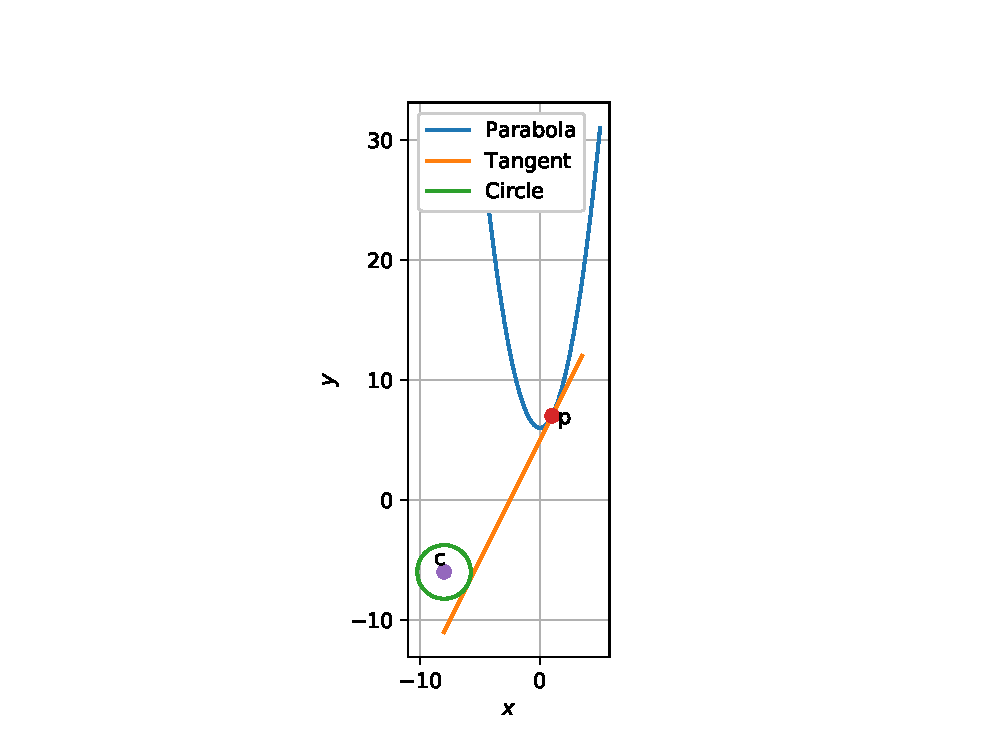
\includegraphics[width=\columnwidth]{./conics/figs/parab.eps}
\caption{}
\label{fig:parab}
\end{figure}

\end{enumerate}
%


\subsection{Affine Transformation}
\renewcommand{\theequation}{\theenumi}
\begin{enumerate}[label=\arabic*.,ref=\thesubsection.\theenumi]
\numberwithin{equation}{enumi}
%
\item In general, Fig. \ref{fig:parab} was generated using an {\em affine transformation}.

\item Express 
\begin{align}
y_2 = y_1^2
\label{eq:parab}
\end{align}
as a matrix equation.
\\
\solution  \eqref{eq:parab} can be expressed as
\begin{align}
\vec{y}^T\vec{D}\vec{y}+2\vec{g}^T\vec{y} = 0
\label{eq:parab_mat}
\end{align}
%
where 
\begin{align}
\vec{D} = \myvec{1 & 0 \\ 0 & 0} 
,
\vec{g} &= -\frac{1}{2}\myvec{0 \\ 1}
\label{eq:parab_coeffs}
\end{align}
%
\item Given 
\begin{align}
\vec{x}^T\vec{V}\vec{x}+2\vec{u}^T\vec{x}+ F = 0,
\label{eq:parab_gen}
\end{align}
where 
\begin{align}
\vec{V}=\vec{V}^T, \det(\vec{V}) = 0,
\label{eq:parab_vcond}
\end{align}
%
and $\vec{P}, \vec{c}$ such that
\begin{align}
\vec{x} = \vec{P}\vec{y}+\vec{c}.
\label{eq:parab_affine}
\end{align}
\eqref{eq:parab_affine} is known as an affine transformation.
Show that
\begin{align}
\begin{split}
\vec{D} &= \vec{P}^T\vec{V}\vec{P}
\\
\vec{g} &= \vec{P}^T\brak{\vec{V}\vec{c}+\vec{u}}
\\
F+ \vec{c}^T\vec{V}\vec{c} + 2\vec{u}^T\vec{c}&= 0
\end{split}
\label{eq:parab_parmas}
\end{align}

\solution Substituting \eqref{eq:parab_affine} in \eqref{eq:parab_gen},
\begin{align}
\brak{\vec{P}\vec{y}+\vec{c}}^T\vec{V}\brak{\vec{P}\vec{y}+\vec{c}}+2\vec{u}^T\brak{\vec{P}\vec{y}+\vec{c}}+ F = 0, 
\end{align}
which can be expressed as
\begin{multline}
\implies \vec{y}^T\vec{P}^T\vec{V}\vec{P}\vec{y}+2\brak{\vec{V}\vec{c}+\vec{u}}^T\vec{P}\vec{y}
\\
+ F+ \vec{c}^T\vec{V}\vec{c} + 2\vec{u}^T\vec{c} = 0
\label{eq:parab_simp}
\end{multline}
%
Comparing \eqref{eq:parab_simp} with \eqref{eq:parab_mat} \eqref{eq:parab_parmas} is obtained.
%
\item Show that there exists a $\vec{P}$ such that 
\begin{align}
\vec{P}^T\vec{P} = \vec{I}
\end{align}
%
Find $\vec{P}$ using
\begin{align}
\vec{D} = \vec{P}^T\vec{V}\vec{P}
\end{align}
\item Find $\vec{c}$ from \eqref{eq:parab_parmas}.
\\
\solution 
\begin{align}
\because \vec{g} &= \vec{P}^T\brak{\vec{V}\vec{c}+\vec{u}},
\\
\vec{V}\vec{c}&= \vec{P}\vec{g} - \vec{u}
\\
\implies \vec{c}^T\vec{V}\vec{c} &= \vec{c}^T\brak{\vec{P}\vec{g} - \vec{u}} = -F- 2\vec{u}^T\vec{c}
\end{align}
%
resulting in the matrix equation
\begin{align}
\myvec{\vec{V}\\ \brak{\vec{P}\vec{g} + \vec{u}}^T}\vec{c}&= \myvec{\vec{P}\vec{g} - \vec{u}\\ -F}
\end{align}
%
for computing $\vec{c}$.
\end{enumerate}



\subsection{Ellipse: Eigenvalues and Eigenvectors}
\renewcommand{\theequation}{\theenumi}
\begin{enumerate}[label=\arabic*.,ref=\thesubsection.\theenumi]
\numberwithin{equation}{enumi}

\item Express the following equation in the form given in \eqref{eq:quad_form}
\begin{equation}
E:\, 5x_1^2-6x_1x_2 + 5x_2^2+22x_1-26x_2+29=0
\label{eq:ellipse}
\end{equation}
\\
\solution \eqref{eq:ellipse} can be expressed as
\begin{equation}
\vec{x}^TV\vec{x} + 2\vec{u}^T\vec{x}  + 29=0
\label{eq:ellipse_quadc}
\end{equation}
%
where
\begin{equation}
V = \myvec{5 & -3 \\ -3 & 5}, \vec{u} = \myvec{11 \\ -13}
\label{eq:ellipsevu}
\end{equation}
%\item Find $\vec{c}$ and $K$ such that 
%\begin{equation}
%\brak{\vec{x}-\vec{c}}^TV\brak{\vec{x}-\vec{c}} = K 
%\label{eq:ellipsec}
%\end{equation}
%%
%\solution \eqref{eq:ellipsec} can be expressed as
%\begin{align}
%\vec{x}^TV\vec{x}-2\vec{c}^TV\vec{x} +\vec{c}^TV\vec{c}-K = 0.
%\end{align}
%%
%Comparing with \eqref{eq:ellipse_quadc},
%\begin{align}
%V\vec{c}&=-\vec{u}
%\\
%\vec{c}^TV\vec{c} - K &=29
%\\
%\implies \vec{c} &=-V^{-1}\vec{u} = \myvec{-1 \\ 2},
%\\
%\text{and }K& = 8
%\end{align}
%
\item Using the affine transformation in \eqref{eq:parab_affine}, show that 
\eqref{eq:ellipse_quadc} can be expressed as
\begin{equation}
\vec{y}^TD\vec{y}= 1
\label{eq:ellipseo}
\end{equation}
%
where
\begin{align}
\label{eq:ellipse_parmas_d}
\vec{D} &= 
\vec{P}^T\vec{V}\vec{P}
\\
\vec{c}&= -\vec{V}^{-1}\vec{u}
\label{eq:ellipse_parmas_c}
\end{align}
for 
\begin{equation}
\vec{P}^\vec{T}\vec{P} = \vec{I}
\label{eq:ellipse_trans}
\end{equation}
\item Find $\vec{c}$
%For 
\\
\solution 
\begin{align}
%\vec{y}= \frac{P^T\brak{\vec{x}-\vec{c}}}{\sqrt{K}},
\vec{c} = \myvec{1 \\ -2}
%\label{eq:ellipse_xy}
\end{align}
%\eqref{eq:ellipsec} transforms to \eqref{eq:ellipseo}.
\item If 
\begin{align}
D &= \myvec{\lambda_1 & 0 \\ 0 & \lambda_2 }
\\
P &= \myvec{\vec{P}_1 & \vec{P}_2 }
\label{eq:ellipse_eigmat}
\end{align}
show that 
\begin{equation}
V\vec{z} = \lambda \vec{z}
\label{eq:ellipse_eig}
\end{equation}
%
where $\lambda \in \cbrak{\lambda_1, \lambda_2}, \vec{z}\in\cbrak{ \vec{P}_1, \vec{P}_2}$.
\item Find $\lambda$.
\\
\solution $\lambda$ is obtained by solving the following equation.
%\item Find the length of the semi-major and semi-minor axes of $E$.
%\\
%\solution The values are given by
%\begin{align}
%\sqrt{\frac{K}{\lambda}}
%\label{eq:ellipsekl}
%\end{align}
%obtained by solving for $\lambda$ in \eqref{eq:ellipse_eig}.  Thus,
\begin{align}
\abs{\lambda I-V} &= 0
\label{eq:ellipse_ceq}
\\
\implies\begin{vmatrix}\lambda -5 & 3 \\ 3 & \lambda -5\end{vmatrix} & = 0
\\
\implies \lambda^2 -10 \lambda+ 16 &= 0
\\
\implies \lambda &= 2, 8
\end{align}
%Thus, the length of the semi-major axis is 2 and that of the semi-minor axis is 1.
\item Sketch \ref{eq:ellipseo}.
\item Find $\vec{P}_1$ and $\vec{P}_2$.
\\
\solution From \eqref{eq:ellipse_eig}
\begin{align}
V\vec{P}_1 &= \lambda_1 \vec{P}_1
\\
\implies \brak{V-\lambda I} \vec{y}&= 0
\\
\implies \myvec{1 & -1} \vec{P}_1&= 0
\\
\text{or, } \vec{P}_1 = k_1 \myvec{1 \\ 1}
\label{eq:ellipsen1}
\end{align}
%
Similarly, 
%where
%\begin{align}
%\vec{n}_1= \myvec{1 \\ -1}
%\end{align}
%
%Similarly, $\vec{P}_2$ is a point on
\begin{align}
\myvec{1 &  1}\vec{P}_2&= 0
\\
\text{or, } \vec{P}_2 = k_2 \myvec{1 \\ -1}
\end{align}
%
%\begin{align}
%\vec{n}_2= 
%\end{align}
\item Find $\vec{P}$.
\\
\solution From \eqref{eq:ellipse_trans} and \eqref{eq:ellipse_eigmat},
\begin{align}
k_1 &=  \frac{1}{\norm{\myvec{1 \\ 1}}} = \frac{1}{\sqrt{2}}
\\
k_2 &=  \frac{1}{\norm{\myvec{1 \\ -1}}} = \frac{1}{\sqrt{2}}
\end{align}
%
Thus,
\begin{align}
\vec{P} = \frac{1}{\sqrt{2}}\myvec{1 & 1 \\ 1 & -1}
\end{align}

\item Find the equation of the major axis for $E$.
\\
\solution  The major axis for \eqref{eq:ellipseo} is the line
\begin{equation}
\vec{y} = \lambda_1\myvec{1 \\ 0}.
\end{equation}
Using the affine transformation in \eqref{eq:parab_affine}
\begin{align}
\vec{x}= \vec{P}\vec{y}+\vec{c}
\\ 
\implies  \vec{x}-\vec{c}= \lambda_1\vec{P}_1
\\ 
\text{or, }\myvec{1 & -1}\vec{x}&= \myvec{1 & -1}\myvec{1 \\ -2}
\\
&= -3
\end{align}
%
since 
\begin{align}
P\myvec{1 \\ 0}=\vec{P}_1\text{ and } \myvec{1 & -1}\vec{P}_1 = 0
\end{align}
%
which is the major axis of the ellipse $E$.
\item Find the minor axis of $E$.
%
\item Let $\vec{F}_1,\vec{F}_2$ be such that
\begin{equation}
\norm{\vec{x}-\vec{F}_1}
+\norm{\vec{x}-\vec{F}_2} =2k
\end{equation}
Find $\vec{F}_1, \vec{F}_2$ and $k$.
\item Summarize all the above computations through a Python script and plot 
the ellipses in \eqref{eq:ellipse} and \eqref{eq:ellipseo}.
\\
\solution The following script plots Fig. \ref{fig:ellipse} using the 
principles of an affine transformation. 
\begin{lstlisting}
codes/2d/ellipse.py
\end{lstlisting}
\begin{figure}[!ht]
\centering
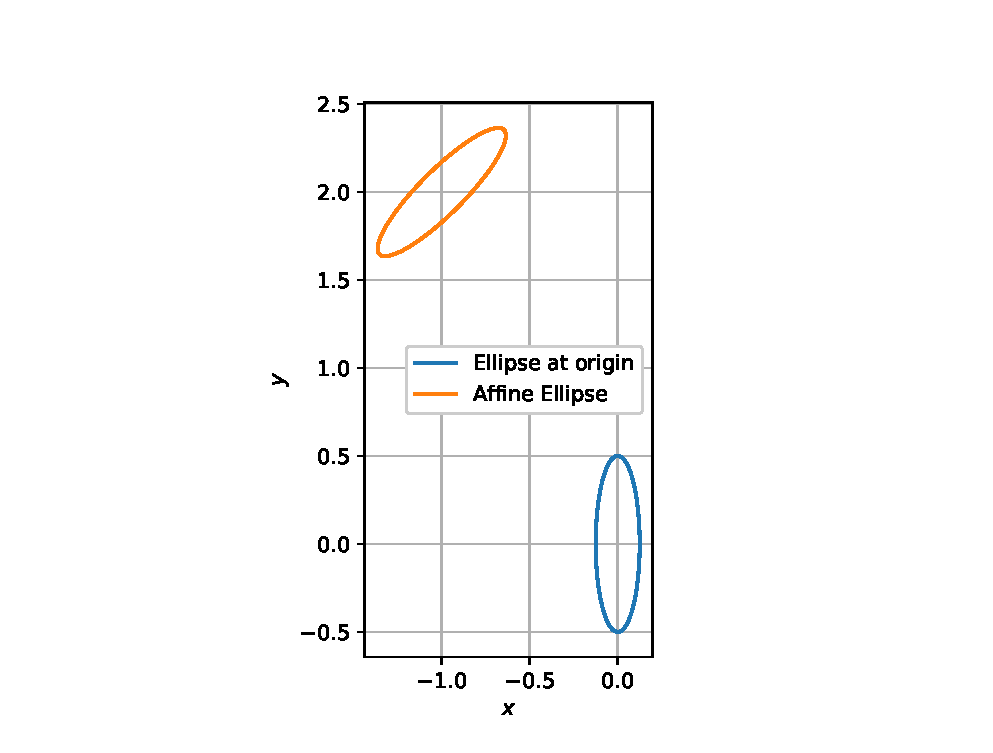
\includegraphics[width=\columnwidth]{./conics/figs/ellipse.eps}
\caption{}
\label{fig:ellipse}
\end{figure}

\end{enumerate}

\subsection{Hyperbola}
\renewcommand{\theequation}{\theenumi}
\begin{enumerate}[label=\arabic*.,ref=\thesubsection.\theenumi]
\numberwithin{equation}{enumi}
\item Tangents are drawn to the hyperbola 
\begin{equation}
\vec{x}^TV\vec{x} =36 
\label{eq:hyper}
\end{equation}
%
where
\begin{equation}
V = \myvec{4 & 0 \\ 0 & -1}
\label{eq:hyperv}
\end{equation}
%
at points $\vec{P}$ and $\vec{Q}$.  If these tangents intersect at 
\begin{equation}
\vec{T}= \myvec{0 \\ 3},
\end{equation}
%
find the equation of $PQ$.
\\
\solution The equations of the two tangents are obtained using \eqref{eq:tangent} as
\begin{align}
\vec{P}^TV\vec{x} &=36
\\
\vec{Q}^TV\vec{x}  &=36.
\end{align}		
%
Since both pass through $\vec{T}$
\begin{align}
\label{eq:hyperp}
\vec{P}^TV\vec{T}  &=36 \implies \vec{P}^T\myvec{0  \\  -3} = 36
\\
\vec{Q}^TV\vec{T}  &=36 \implies \vec{Q}^T\myvec{0  \\  -3} = 36
\label{eq:hyperq}
\end{align}
Thus, $\vec{P}, \vec{Q}$ satisfy
\begin{align}
\myvec{0 &  -3}\vec{x} &= -36
\\
\implies \myvec{0 &  1}\vec{x} &= -12
\label{eq:d1}
\end{align}
%
which is the equation of $PQ$.
\item In $\triangle PTQ$, find the equation of the altitude $TD \perp PQ$.
\\
\solution Since 
\begin{align}
 \myvec{1 &  0} \myvec{0 \\  1}=0
\end{align}
using \eqref{eq:line_normal} and \eqref{eq:d1},
the equation of $TD$ is
\begin{align}
\myvec{1 & 0}\brak{\vec{x}-\vec{T}} &= 0
\\
\implies \myvec{1 & 0}\vec{x} &= 0
\label{eq:d2}
\end{align}
%
\item Find $D$.
\\
\solution
From \eqref{eq:d1} and \eqref{eq:d2},
\begin{align}
 \myvec{1 & 0 \\ 0 &  1}\vec{D} &= \myvec{0 \\ -12 }
\\
\implies  \vec{D} &= \myvec{0 \\ -12 }
\label{eq:hyperd}
\end{align}
%
\item Show that the equation of $PQ$ can also be expressed as
\begin{align}
\label{eq:pq_slope}
\vec{x} = \vec{D}+\lambda \vec{m}
\end{align}
where
\begin{align}
\vec{m} &=   \myvec{1 \\ 0}
\label{eq:hyper_slope}
\end{align}
%
\item Show that for $\vec{V}^T = \vec{V}$,
\begin{equation}
\label{eq:quad_md}
\brak{\vec{D}+\lambda\vec{m}}^TV\brak{\vec{D}+\lambda\vec{m}} + F= 0 
\end{equation}
can be expressed as
\begin{equation}
\label{eq:quad_lambda}
\lambda^2\vec{m}^TV\vec{m}+2\lambda\vec{m}^TV\vec{D}+\vec{D}^TV\vec{D}
+ F = 0
\end{equation}
%
\item Find $\vec{P}$ and $\vec{Q}$.
\\
\solution From \eqref{eq:pq_slope} and \eqref{eq:hyper} \eqref{eq:quad_lambda} is obtained.
%
Substituting from \eqref{eq:hyper_slope}, \eqref{eq:hyperv} and \eqref{eq:hyperd}
\begin{align}
\vec{m}^TV\vec{m} &= \myvec{1& 0} \myvec{4 & 0 \\ 0 & -1}\myvec{1 \\ 0} = 4
\\
\vec{m}^TV\vec{D} & = \myvec{1& 0}\myvec{4 & 0 \\ 0 & -1}\myvec{0 \\ -12 } = 0
\\
\vec{D}^TV\vec{D} &= \myvec{0 & -12 }\myvec{4 & 0 \\ 0 & -1}\myvec{0 \\ -12 } = -144
\end{align}
%
Substituting in \eqref{eq:quad_lambda}
\begin{align}
4 \lambda^2 - 144 &= 36
\\
\implies
\lambda &= \pm 3\sqrt{5}
\end{align}
%
Substituting in \eqref{eq:pq_slope},
\begin{align}
\vec{P} &= \vec{D}+ 3\sqrt{5} \vec{m} = 3 \myvec{ \sqrt{5} \\ -4}
\\
\vec{Q} &= \vec{D}- 3\sqrt{5} \vec{m} = -3 \myvec{ \sqrt{5} \\ 4}
\end{align}
%
\item Find the area of $\triangle PTQ$.
\\
\solution Since
\begin{align}
PQ &= \norm{\vec{P}-\vec{Q}} = 6\sqrt{5}
\\
TD &= \norm{\vec{T}-\vec{D}} = 15,
\end{align}
the desired area is
\begin{equation}
\frac{1}{2}PQ \times TD = 45 \sqrt{5}
\end{equation}
\item Repeat the previous exercise using determinants.
\item Summarize all the above computations through a Python script and plot 
the hyperbola.
\end{enumerate}

\subsection{Karush-Kuhn-Tucker (KKT) Conditions}
\renewcommand{\theequation}{\theenumi}
\begin{enumerate}[label=\arabic*.,ref=\thesubsection.\theenumi]
\numberwithin{equation}{enumi}

\item
Solve
 \begin{align}
 \label{ch2_kkt_problem}
\min_{\mbf{x}} f\brak{\mbf{x}} = \vec{x}^T\myvec{4 & 0 \\0 & 2}\vec{x}
%4x_1^2 + 2x_2^2
 \end{align}
 with constraints
 \begin{align}
 g_1\brak{\mbf{x}} = \myvec{3 & 1}\vec{x}-8 = 0\\
 g_2 \brak{\mbf{x}}= 15 - \myvec{2 & 4}\vec{x} \geq 0
 \end{align}
 
%
\solution Considering the Lagrangian
%
\begin{align}
%L\brak{\mbf{x},\lambda} &= f\brak{\mbf{x}} + \lambda g_1\brak{\mbf{x}} - \mu g_2\brak{\mbf{x}} \\
% &= 4x_1^2 + 2x_2^2 + \lambda \brak{3x_1 + x_2-8} 
% \nonumber \\
% &\,-\mu\brak{15 - 2x_1 - 4x_2},\\
 \nabla L\brak{\mbf{x},\lambda, \mu}  %& = 
%\begin{pmatrix}
%8x_1 + 3 \lambda  +2 \mu  \\
%4x_2 + \lambda + 4 \mu \\
%3x_1 + x_2 -8 \\
% - 2x_1 - 4x_2 + 15
%\end{pmatrix}
= 0
\end{align}
%
resulting in the matrix equation
%
\begin{align}
\Rightarrow 
\begin{pmatrix}
8 &0 & 3 & 2\\
0 &4 & 1 & 4 \\
3 & 1 & 0 &0  \\
2 & 4 & 0 & 0
\end{pmatrix}
\begin{pmatrix}
x_1 \\
x_2 \\
\lambda
\\
\mu
\end{pmatrix}
&=
\begin{pmatrix}
0 \\
0 \\
8 \\
15
\end{pmatrix}
\\
\Rightarrow 
\begin{pmatrix}
x_1 \\
x_2 \\
\lambda
\\
\mu
\end{pmatrix}
&= 
\begin{pmatrix}
1.7 \\
 2.9 \\
-3.12 \\
-2.12
\end{pmatrix}
\end{align}
%
using the following python script.  The (incorrect) graphical solution is available in Fig. \ref{fig.2.12}
%	
\begin{lstlisting}
codes/optimization/2.12.py
\end{lstlisting}

%
Note that $\mu < 0 $, contradicting the necessary condition in \eqref{ch2_kkt_necessary}. 
%
\begin{figure}[!ht]
\centering
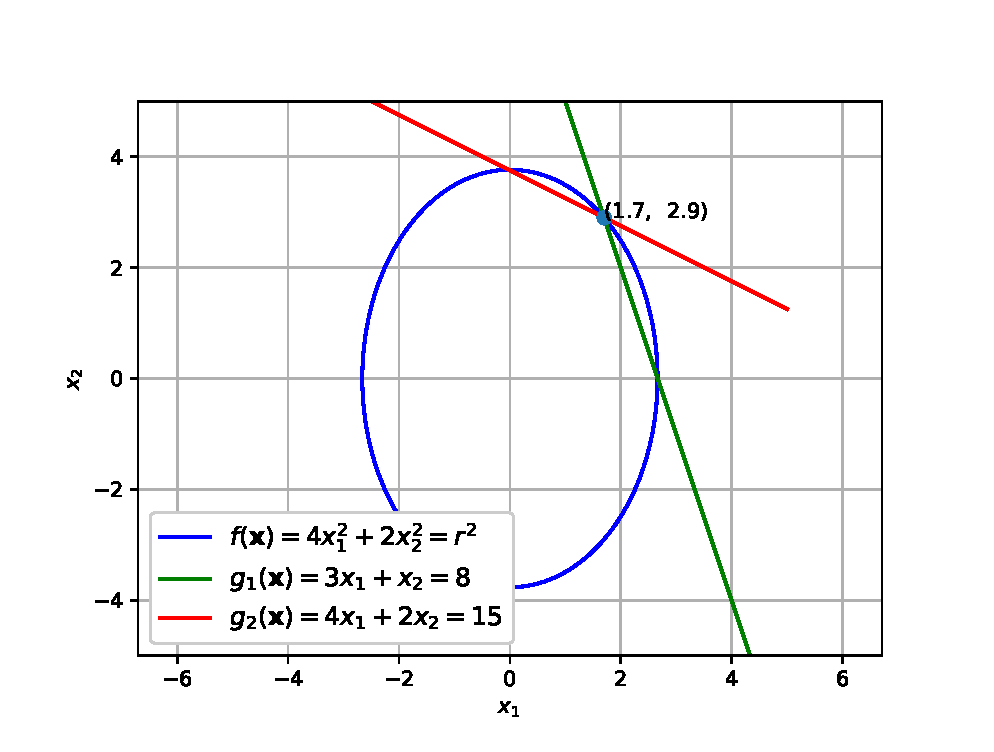
\includegraphics[width=\columnwidth]{./optimization/figs/2.12_1.eps}
\caption{ Incorrect solution is at intersection of all curves $r = 5.33$}
\label{fig.2.12}	
\end{figure}
\item
Obtain the correct solution to the previous problem by considering $\mu = 0$.

\begin{figure}[!ht]
\centering
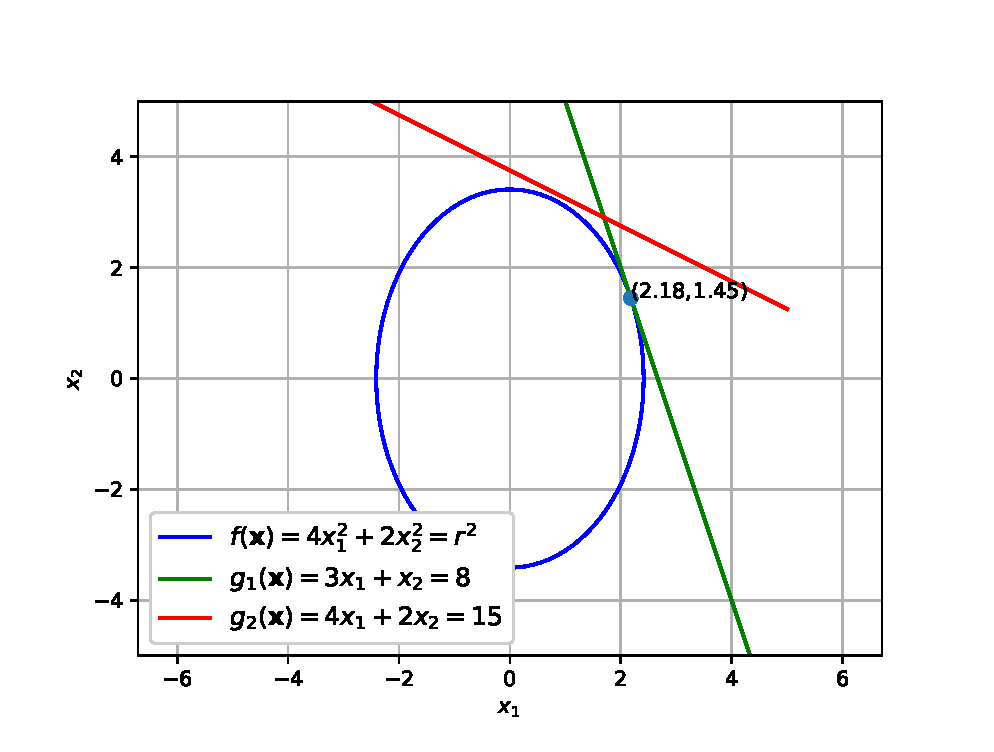
\includegraphics[width=\columnwidth]{./optimization/figs/2.12_2.eps}
\caption{ Optimal solution is where $g_1(x)$ touches the curve $r = 4.82$}
\label{fig.2.13}	
\end{figure}
%
%
\item
Solve
 \begin{align}
% \label{ch2_kkt_problem}
\min_{\mbf{x}} f\brak{\mbf{x}} %= 4x_1^2 + 2x_2^2
 \end{align}
 with constraints
 \begin{align}
 g_1\brak{\mbf{x}} 
%= 3x_1 + x_2-8 
= 0\\
 g_2 \brak{\mbf{x}}
%= 15 - 2x_1 - 4x_2 
\leq 0
 \end{align}
 
%
\item
Based on whatever you have done so far,	list the steps that you would use in general for solving a convex optimization problem  like \eqref{ch2_kkt_problem}  using Lagrange Multipliers. 
These are called Karush-Kuhn-Tucker(KKT) conditions.

\solution For a problem defined by 
\begin{align}
\mbf{x^*} &= \min_{\mbf{x}}f(\mbf{x})
\\
\text{subject to } h_i(\mbf{x}) &= 0, \forall i=1,..,m
\\
\text{subject to } g_i(\mbf{x}) &\le 0, \forall i=1,..,n
\end{align}
%
the optimal solution is obtained through
%
\begin{align}
\mbf{x^*} &= \min_{\mbf{x}}L(\mbf{x}, \mbf{\lambda}, \mbf{\mu}) 
\\
&= \min_{\mbf{x}}f(\mbf{x})  + \underset{i=1}{\overset{m}{\sum}} \lambda_i h_i(\mbf{x}) + \underset{i=1}{\overset{n}{\sum}} \mu_i g_i(\mbf{x}),
\end{align}
%
using the KKT conditions
%
\begin{align}
\Rightarrow \nabla_\mbf{x} f(\mbf{x})  + \underset{i=1}{\overset{m}{\sum}} \nabla_\mbf{x} \lambda_i h_i(\mbf{x}) + \underset{i=1}{\overset{n}{\sum}} \mu_i \nabla_\mbf{x} g_i(\mbf{x}) = 0 
\\
\text{subject to }\mu_i g_i(\mbf{x}) = 0, \forall i = 1,..,n
\\
\text{and }\mu_i \ge 0, \forall i = 1,..,n
\end{align}
%
%
\item
	Maxmimize 
	%
	\begin{align}
	f(\mbf{x}) &= \sqrt{x_1x_2}
	\end{align}
	%
	with the constraints
	%
	\begin{align}
	x_1^2+x_2^2 &\leq 5 \\
	x_1 \geq 0, x_2 &\geq 0
	\end{align}
	%
\end{enumerate}

 
\subsection{Solved Problems}
\renewcommand{\theequation}{\theenumi}
\begin{enumerate}[label=\arabic*.,ref=\thesubsection.\theenumi]
\numberwithin{equation}{enumi}
\item Two parabolas with a common vertex and with axes along $x$-axis and $y$-axis, respectively, intersect 
each other in the first quadrant.  If the length of the latus rectum of each parabola is 3, find the equation 
of the common tangent to the two parabolas.
\\
\solution The equation of a conic is given by 
%
\begin{align}
\label{eq:conic_gen}
\vec{x}^T\vec{V}\vec{x}+2\vec{u}^T\vec{x}+F=0
\end{align}
%
For the standard parabola, 
\begin{align}
\label{eq:conic_parab_V}
\vec{V}&=\myvec{0 & 0 \\ 0& 1}
\\
\vec{u}&=-2a\myvec{1 \\ 0}
\label{eq:conic_parab_u}
\\
F&=0
\label{eq:conic_parab_const}
\end{align}
%
The focus
\begin{align}
\label{eq:conic_parab_focus}
\vec{F}&=a\myvec{1 \\ 0}
\end{align}
%
The Latus rectum is the line passing through $\vec{F}$ with direction vector 
\begin{align}
\label{eq:conic_parab_latus_m}
\vec{m}&=\myvec{0 \\ 1}
\end{align}
%
Thus, the equation of the Latus rectum is 
\begin{align}
\label{eq:conic_parab_latus}
\vec{x}&= \vec{F}+\lambda \vec{m}
\end{align}
%
The intersection of the latus rectum and the parabola is obtained from \eqref{eq:conic_parab_const}
, \eqref{eq:conic_parab_latus}
and \eqref{eq:conic_gen} as
\begin{align}
\brak{\vec{F}+\lambda \vec{m}}^T\vec{V}\brak{\vec{F}+\lambda \vec{m}}+2\vec{u}^T\brak{\vec{F}+\lambda \vec{m}}=0
\end{align}
\begin{multline}
\label{eq:conic_parab_lam_quad}
\implies \brak{\vec{m}^T\vec{V}\vec{m}}\lambda^2+2\brak{\vec{V}\vec{F}+\vec{u}}^T\vec{m}\lambda 
\\
+\brak{\vec{V}\vec{F}+2\vec{u}}^T\vec{F} = 0
\end{multline}
From \eqref{eq:conic_parab_V}, \eqref{eq:conic_parab_u}, \eqref{eq:conic_parab_focus} and \eqref{eq:conic_parab_latus_m}, 
\begin{align}
\label{eq:conic_parab_lam_a}
\vec{m}^T\vec{V}\vec{m} &= 1
\\
\label{eq:conic_parab_lam_b}
\brak{\vec{V}\vec{F}+\vec{u}}^T\vec{m} &= 0
\\
\brak{\vec{V}\vec{F}+2\vec{u}}^T\vec{F} &= -4a^2
\label{eq:conic_parab_lam_c}
\end{align}
Substituting from \eqref{eq:conic_parab_lam_a}, \eqref{eq:conic_parab_lam_b}  and \eqref{eq:conic_parab_lam_c} in \eqref{eq:conic_parab_lam_quad}, 
\begin{align}
\lambda^2  - 4a^2 &=0
\\
\implies \lambda_1 &=2a,\lambda_2 =-2a
\label{eq:conic_parab_latus_lam}
\end{align}
%
Thus, from \eqref{eq:conic_parab_latus_m}, \eqref{eq:conic_parab_latus}
 and \eqref{eq:conic_parab_latus_lam}, the length of the latus rectum is
\begin{align}
\brak{\lambda_1-\lambda_2} \norm{\vec{m}} = 4a
\end{align}
%
From the given information, the two parabolas $P_1, P_2$ have parameters
\begin{align}
\label{eq:conic_parab_param1}
\vec{V}_1&=\myvec{0 & 0 \\ 0& 1},\vec{u}_1=-2a\myvec{1 \\ 0},F_1=0
\\
\label{eq:conic_parab_param2}
\vec{V}_2&=\myvec{1 & 0 \\ 0& 0},
\vec{u}_2=-2a\myvec{0 \\ 1},
F_2=0
\\
4a&=3
\label{eq:conic_parab_a}
\end{align}
Let $L$ be the common tangent for $P_1,P_2$ with  $\vec{c},\vec{d}$ being the respective points of contact. The respectivel normal vectors are
\begin{align}
\vec{n}_1 &= \vec{V}_1\vec{c}+\vec{u}_1 = -2a\myvec{1\\-\frac{c_2}{2a}}
\\
\vec{n}_2 &= \vec{V}_2\vec{d}+\vec{u}_2  = d_1\myvec{1\\-\frac{2a}{d_1}}
\end{align}
%
From the above equations, since both normals have the same direction vector, 
\begin{align}
\myvec{1\\-\frac{c_2}{2a}}&=\myvec{1\\-\frac{2a}{d_1}}
\implies c_2d_1 = 4a^2
\end{align}
%Also, 
%\begin{align}
%d_2 = 4ad_1^2, c_1 = 4ac_2^2
%\end{align}
%Thus,
%\begin{align}
%\vec{c} = \myvec{\frac{64a^5}{d_1^2}\\ \frac{4a^2}{d_1}}, \vec{d} = \myvec{d_1\\ 4ad_1^2}
%\end{align}

%\item A hyperbola passes through the point 
%\begin{equation}
%\vec{P}=\myvec{\sqrt{2}\\ \sqrt{3}}
%\end{equation}
%and has foci at $\myvec{\pm 2\\ 0}$.  Find the equation of the tangent to this hyperbola at 
%$\vec{P}$.
%\\
%\solution Let 
%\begin{align}
%\vec{F}_1 = 2\myvec{1 \\ 0},
%\vec{F}_2 = -2\myvec{1 \\ 0}
%\end{align}
%%
%Comparing with \eqref{eq:conic_gen}
%%
%\begin{align}
%\vec{V} &= \myvec{\frac{1}{a^2} & 0 \\ 0 & -\frac{1}{b^2}}, 
%\vec{u} = 0,
%F=-1,
%\\
%  a^2+b^2 &= 4
%\end{align}
%%
%The equation to the tangent is then given by 
%\begin{align}
%\brak{\vec{\vec{V}\vec{P}}}^T\vec{x} &= 1
%\implies \myvec{\frac{\sqrt{2}}{a^2} & -\frac{\sqrt{3}}{b^2}}\vec{x} &=1
%\end{align}

\item Find the product of the perpendiculars drawn from the foci of the ellipse
\begin{equation}
\label{eq:ellipse_prod}
\vec{x}^T\myvec{25 & 0 \\ 0 & 9}\vec{x}  = 225
\end{equation}
upon the tangent to it at the point
\begin{equation}
\frac{1}{2}\myvec{3\\ 5 \sqrt{3}}
\end{equation}
\\
\solution For the ellipse in \eqref{eq:ellipse_prod},
\begin{align}
\label{eq:ellipse_prod_param}
V = \myvec{\frac{1}{9} & 0 \\ 0 & \frac{1}{25}}, \vec{u} = 0, F=-1
\end{align}
%
The equation of the desired tangent is
\begin{align}
\label{eq:ellipse_prod_tangent}
\brak{\vec{V}\vec{P}}^T\vec{x}&=1
\\
\implies \myvec{\frac{1}{3} & \frac{\sqrt{3}}{5}}\vec{x}&=2
\end{align}
%
The foci of the ellipse are located at
\begin{align}
\vec{F}_1 = \myvec{0\\4},
\vec{F}_2 = \myvec{0\\-4}
\end{align}
The product of the perpendiculars is
\begin{align}
\frac{\abs{\myvec{\frac{1}{3} & \frac{\sqrt{3}}{5}}\myvec{0\\4}-2}\abs{\myvec{\frac{1}{3} & \frac{\sqrt{3}}{5}}\myvec{0\\-4}-2}}{\norm{\myvec{\frac{1}{3} & \frac{\sqrt{3}}{5}}}^2}
=9
\end{align}

\item  Consider an ellipse, whose centre is at the origin and its major axis is along the $x$-axis.  If its 
eccentricity is $\frac{3}{5}$ and the distance between its foci is 6, then find the area of the quadrilateral 
inscribed in the ellipse,  with the vertices as the vertices of the ellipse.
\\
\solution If $a$ and $b$ be the semi-major and minor-axis respectively, 
the foci of the ellipse are 
\begin{align}
\vec{F}_1=ae\myvec{1\\0},
\vec{F}_2=-ae\myvec{1\\0}
\end{align}
%
From the given information,
\begin{align}
e &= \frac{3}{5}, 2ae = 6 
\\
\implies a &= 5, b = a\sqrt{1-e^2} = 4
\end{align}
%
Thus, the vertices of the ellipse are
\begin{align}
\myvec{a\\0},
\myvec{-a\\0},
\myvec{0\\b},
\myvec{0\\-b}
\end{align}
and the area of the quadrilateral is
\begin{align}
\frac{1}{2}
\begin{vmatrix}
1 & 1 & 1
\\
a & -a & 0
\\
0 & 0 & b
\end{vmatrix}
+
\frac{1}{2}
\begin{vmatrix}
1 & 1 & 1
\\
a & -a & 0
\\
0 & 0 & -b
\end{vmatrix}
=2ab = 40
\end{align}

\item Let $a$ and $b$ respectively be the semi-transverse and semi-conjugate axes of a hyperbola whose 
eccentricity satisfies the equation
\begin{equation}
\label{eq:hyper_ecc}
9e^2-18e+5 = 0
\end{equation}
If 
\begin{equation} 
\label{eq:hyper_ecc_focus}
\vec{S}=\myvec{5\\ 0}
\end{equation}
is a focus and 
\begin{equation} 
\label{eq:hyper_ecc_direc}
\myvec{5 & 0}\vec{x} = 9
\end{equation} 
%
is the corresponding directrix of this hyperbola, then find $a^2-b^2$.
\\
\solution From \eqref{eq:hyper_ecc},
\begin{align}
\brak{3e-1}\brak{3e-5} = 0
\\
\implies e = \frac{5}{3}, \because e > 1
\label{eq:hyper_ecc_e}
\end{align}
%
for a hyperbola.  
Let $\vec{x}$ be a point on the hyperbola.  
From \eqref{eq:hyper_ecc_direc}, its distance from the directrix is
%
\begin{align}
\label{eq:hyper_ecc_direc_dist}
\frac{\abs{\myvec{5 & 0}\vec{x} - 9}}{5}
\end{align}
%
and from the focus is 
\begin{align}
\label{eq:hyper_ecc_focus_dist}
\norm{\vec{x}-\myvec{5\\0}}
\end{align}
From the definition of a hyperbola, the eccentricity is the ratio of these distances and \eqref{eq:hyper_ecc_e}
, \eqref{eq:hyper_ecc_direc_dist}
 and \eqref{eq:hyper_ecc_focus_dist},
\begin{align}
\frac{5\norm{\vec{x}-\myvec{5\\0}}}{\abs{\myvec{5 & 0}\vec{x} - 9}} &= \frac{5}{3}
\\
\implies 9\cbrak{\brak{x_1-5}^2+x_2^2}&=  \brak{5x_1-9}^2
\\
\text{or, } \vec{x}^T\myvec{16 & 0 \\ 0 & -9}\vec{x} = 225
\end{align}
%
which is the equation of the hyperbola.  Thus, 
\begin{align}
a^2 = \frac{225}{16}, b^2 = \frac{225}{9}
\\
\implies a^2-b^2 = -\frac{175}{16}
\end{align}


%From \eqref{eq:hyper_ecc_focus},
%\begin{align}
%ae = 5 \implies a= 3
%\end{align}

\item A variable line drawn through the 
intersection of the lines 
\begin{align} 
\label{lines_3}
\myvec{4 & 3}\vec{x} &=12 
\\ 
\myvec{3 & 4}\vec{x} &=12 
\end{align} 
meets the coordinate axes at $\vec{A}$ and $\vec{B}$, then find the locus of the midpoint of $AB$. 
\\
\solution The intersection of the lines in \eqref{lines_3} is obtained through the matrix equation 
\begin{align}
\myvec{4 & 3 \\ 3 & 4}\vec{x}  &=\myvec{12\\12}
\end{align}
by forming the augmented matrix and row reduction as  
\begin{align}
\myvec{4 & 3 &12 \\ 3 & 4 &12} &\leftrightarrow \myvec{4 & 3 &12 \\ 0 & 7 &12} \leftrightarrow \myvec{28 & 0 & 48 \\ 0 & 7 &12}
\nonumber \\
\leftrightarrow \myvec{7 & 0 & 12 \\ 0 & 7 &12}&
\end{align}
resulting in 
\begin{align}
\vec{C}=\frac{1}{7}\myvec{12\\12}
\end{align}
%
Let the $\vec{R}$ be the mid point of $AB$. Then,
\begin{align}
\label{eq:lines_3_abr}
\vec{A} =2 \myvec{1 & 0\\0 & 0}\vec{R} 
\\
\vec{B} =2 \myvec{0 & 0\\0 & 1}\vec{R} 
\end{align}
%
Let the equation of $AB$ be 
%equation of a line passing through $\vec{C}$ be 
\begin{align}
\vec{n}^T\brak{\vec{x} - \vec{C}} = 0
\label{eq:lines_3_def}
\end{align}
Since $\vec{R}$ lies on $AB$, 
\begin{align}
\vec{n}^T\brak{\vec{R} - \vec{C}} = 0
\label{eq:lines_3_rc}
\end{align}
Also, 
\begin{align}
\vec{n}^T\brak{\vec{A} - \vec{B}} = 0
\label{eq:lines_3_ab}
\end{align}
%
Substituting from \eqref{eq:lines_3_abr} in \eqref{eq:lines_3_ab},
\begin{align}
\vec{n}^T\myvec{1 & 0 \\ 0 & -1}\vec{R} = 0
\label{eq:lines_3_r_sub}
\end{align}
%
From \eqref{eq:lines_3_rc} and \eqref{eq:lines_3_r_sub},
\begin{align}
\brak{\vec{R} - \vec{C}} = k\myvec{1 & 0 \\ 0 & -1}\vec{R}
\label{eq:lines_3_k}
\end{align}
%
for some constant $k$.
Multiplying both sides of \eqref{eq:lines_3_k} by 
\begin{align}
\vec{R}^T\myvec{0 & 1 \\ 1 & 0},
\end{align}
\begin{align}
\vec{R}^T\myvec{0 & 1 \\ 1 & 0}\brak{\vec{R} - \vec{C}} &= k\vec{R}^T\myvec{0 & 1 \\ 1 & 0}\myvec{1 & 0 \\ 0 & -1}\vec{R}
\nonumber \\
&= k\vec{R}^T\myvec{0 & -1 \\ 1 & 0}\vec{R} = 0
\label{eq:lines_3_mul}
\end{align}
\begin{align}
\because \vec{R}^T\myvec{0 & -1 \\ 1 & 0}\vec{R} = 0
\end{align}
which can be easily verified for any $\vec{R}$.
%
from \eqref{eq:lines_3_mul},
\begin{align}
\vec{R}^T\myvec{0 & 1 \\ 1 & 0}\brak{\vec{R} - \vec{C}} = 0
\nonumber \\
\implies \vec{R}^T\myvec{0 & 1 \\ 1 & 0}\vec{R} - \vec{R}^T\myvec{0 & 1 \\ 1 & 0}\vec{C} = 0
\nonumber \\
\implies \vec{R}^T\myvec{0 & 1 \\ 1 & 0}\vec{R} - \vec{C}^T\myvec{0 & 1 \\ 1 & 0}\vec{R} = 0
\end{align}
%
which is the desired locus.
\end{enumerate}
 
\subsection{JEE Exercises}
\renewcommand{\theequation}{\theenumi}
\begin{enumerate}[label=\arabic*.,ref=\thesubsection.\theenumi]
\numberwithin{equation}{enumi}

\item Find the point of intersection of the tangents at the ends of the latusrectum of the parabola
\begin{align} 
\vec {x}^T \myvec{0 & 0 \\ 0 & 1} \vec {x}=\myvec{4&0}\vec {x}.
\end{align} 
\item An ellipse has eccentricity $\frac{1}{2}$ and one focus at the point $\vec{P}=\myvec{\frac{1}{2}\\1}$. Its one directrix is the common tangent, nearer to the point $\vec{P}$, to the circle 
    \begin{align}
    \vec {x}^T \vec {x} =1
    \end{align} and the hyperbola 
    \begin{align}
    \vec {x}^T \myvec{1& 0 \\0 &-1}\vec {x}=1.
    \end{align} Find the equation of the ellipse.
\item The equation 
    \begin{align}
    \vec {x}^T \myvec  {\frac{1}{1-r} & 0 \\ 0 &-\frac {1}{1+r}}\vec{x} = 1, r>1
    \end{align} represents
    \begin{enumerate}
    \item an ellipse
    \item a hyperbola
    \item a circle
    \item none of these
    \end{enumerate} 
    \item Each of the four inequalities given below defines a region in the xy plane. One of these four regions does not have the following property. For any two points \myvec{x_1\\y_1} and \myvec{x_2\\y_2} in the region, the point \myvec{\frac{x_1+x_2}{2}\\ \frac{y_1+y_2}{2}} is also in the region. Find the inequality defining this region.
    \begin{enumerate}
    \item $\vec {x}^T\myvec{1&0 \\0 &2}\vec {x} \leq1$
    \item Max$\myvec{\abs{x} \\ \abs{y}} \leq1$
    \item $\vec {x}^T \myvec{1&0 \\0 &-1}\vec {x} \leq1$
    \item $\vec {x}^T \myvec{0 &0 \\ 0& 1 } + \myvec{-1& 0}\vec {x}\leq0$
    \end{enumerate}    
\item The equation 
\begin{align}
\vec{x}^T \myvec{2&0 \\ 0& 3}\vec{x} + \myvec{-8&-18}\vec{x}+35=k
\end{align} represents
    \begin{enumerate}
    \item no locus if $k>0$
    \item an ellipse if$k<0$
    \item a point if k=0
    \item a hyperbola if $k>0$
    \end{enumerate}
\item Let E be the ellipse 
\begin{align}
\vec {x}^T \myvec {\frac{1}{9}&0 \\ 0&\frac{1}{4}}\vec {x}=1
\end{align} and C be the circle 
\begin{align}
\vec {x}^T \vec {x}=9.
\end{align} let $\vec{P}$ and $\vec{Q}$ be the points  \myvec{1\\2} and \myvec{2\\1} respectively. Then
    \begin{enumerate}
    \item Q lies inside C but outside E.
    \item Q lies outside both C and E. 
    \item P lies inside both C and E. 
    \item P lies inside C but outside E.
    \end{enumerate}
\item Consider a circle with its center lying on the focus of the parabola 
	\begin{align}
	\vec {x}^T \myvec {0&0 \\ 0&1}\vec {x}=\myvec{2p&0}\vec{x}
	\end{align}
	such that it touches the directrix of the parabola. Then find the point of intersection.
\item Find the radius of the circle passing through the foci of the ellipse 
	\begin{align}
	\vec {x}^T \myvec {\frac{1}{16}&0 \\ 0&\frac{1}{9}}\vec {x}=1,
	\end{align} and having its centre at \myvec{0\\3}. 
\item Let $\vec{P} = \myvec{a\sec\theta \\ b\tan\theta}$
	and $\vec{Q}=\myvec{a\sec\phi \\ b\tan\phi}$ where $\theta+\phi=\frac{\pi}{2}$, be two points on  the hyperbola 
    \begin{align}
    \vec{x}^T \myvec{ \frac{1}{a^2}&0 \\ 0&\frac{-1}{b^2}}\vec {x}=1
    \end{align}. If \myvec{h\\k} is the point of intersection of the normals at $\vec{P}$ and 
    $\vec{Q}$, then find k.
\item If 
	\begin{align}
    \myvec{1&0}\vec {x}=9
    \end{align} is the chord of contact of the hyperbola 
    \begin{align}
    \vec {x}^T \myvec {1&0 \\ 0&-1}\vec {x}=9
    \end{align} then find the equation of the corresponding pair of tangents.
\item The curve describes parametrically by 
    \begin{align}
    \myvec{1&0}\vec {x}=t^2+t+1\\
    \myvec{0&1}\vec {x}=t^2-t+1
    \end{align} represents
    \begin{enumerate}
    \item a pair of straight lines 
    \item an ellipse
    \item a parabola
    \item a hyperbola
    \end{enumerate}
\item If 
	\begin{align}
    \myvec{1&1}\vec{x}=k
    \end{align} is normal to 
    \begin{align}
    \vec {x}^T\myvec{0 & 0 \\0 & 1} \vec{x}=\myvec{12&0}\vec{x},
    \end{align} then find k.
\item If the line 
    \begin{align}
    \myvec{1&0}\vec{x}-1=0
    \end{align}is the directrix of the parabola 
    \begin{align}
    \vec{x}^T \myvec{0 & 0 \\0 & 1}\vec{x}-\myvec{k&0}\vec{x}+8=0,
    \end{align}then find k. 
\item Find the equation of the common tangent touching the circle 
    \begin{align}
    \vec {x}^T\myvec{1 & 0 \\0 & 1}\vec{x}-\myvec{6&0}\vec{x} =0
    \end{align} and the parabola 
    \begin{align}\vec{x}^T \myvec{0 & 0 \\0 & 1}\vec{x}=\myvec{4&0}\vec{x}.
    \end{align}
\item Find the equation of the directrix of the parabola 
    \begin{align}
    \vec{x}^T\myvec{0 & 0 \\0 & 1}\vec{x}+\myvec{4&4}\vec{x}+2=0.
    \end{align}
\item If $a>2b>0$ then the positive value of m for which 
	\begin{align}
    \myvec{0&1}\vec {x}=\myvec{m&0}\vec {x}-b\sqrt{1+m^2}
    \end{align} is the common tangent to 
    \begin{align}
    \vec {x}^T\myvec{1 & 0 \\0 & 1}\vec{x}=b^2\\ 
    \vec {x}^T\myvec {1 & 0 \\0 &1}\vec{x}+\myvec{2a&0}\vec{x}=a^2-b^2
    \end{align} is 
    \begin{enumerate}
    \item $\frac{2b}{\sqrt{a^2-4b^2}}$
    \item $\frac{\sqrt{a^2-4b^2}}{2b}$
    \item $\frac{2b}{a-2b}$
    \item $\frac{b}{a-2b}$
    \end{enumerate}
\item The locus of the mid-point of the line segment joining the focus to a moving point on the 			parabola  
    \begin{align} 
    \vec {x}^T\myvec{0 & 0 \\0 & 1}\vec {x}=\myvec{4a&0}\vec{x}
    \end{align} is another parabola with directrix 
    \begin{enumerate}
    \item $\myvec{1&0}\vec{x}=-a$
    \item $\myvec{1&0}\vec{x}=\frac{-a}{2}$
    \item $\myvec{1&0}\vec{x}=0$
    \item $\myvec{1&0}\vec{x}=\frac{a}{2}$
    \end{enumerate}
\item Find the equation of the common tangent to the curves 
	\begin{align}
    \vec{x}^T \myvec{0 & 0 \\0 & 1}\vec{x}=\myvec{8&0}\vec{x}\\
    \vec{x}^T \myvec{0 & 0 \\ 1& 0}\vec{x}=-1
    \end{align}
\item Find the area of the quadrilateral formed by the tangents at the end points of latusrectum to the ellipse
    \begin{align}
    \vec{x}^T \myvec{\frac{1}{9} & 0 \\0 & \frac{1}{5}} \vec{x}=1.
    \end{align}
\item The focal chord to
    \begin{align}
    \vec{x}^T \myvec{0 & 0 \\0 & 1}\vec{x}=\myvec{16&0}\vec{x}
    \end{align}
    is tangent to
    \begin{align}
    \vec {x}^T\vec{x}-\myvec{12&0}\vec{x}+36=0
    \end{align} then the possible values of the slope of the chord,are 
    \begin{enumerate}
    \item $\myvec{-1\\1}$
    \item $\myvec{-2\\2}$
    \item $\myvec{-2\\ -\frac{1}{2}}$
    \item $\myvec{2\\ -\frac{1}{2}}$
    \end{enumerate}
\item For hyperbola 
    \begin{align} 
    \vec {x}^T\myvec {\frac{1}{\cos^2\alpha} & 0 \\0 & -\frac{1}{\sin^2\alpha}} \vec{x}=1
    \end{align} which of the following remains constant with change in $'\alpha'$
    \begin{enumerate}
    \item abscissae of vertices
    \item abscissae of foci
    \item eccentricity
    \item directrix
    \end{enumerate}
\item If tangents are drawn to the ellipse 
    \begin{align}
    \vec{x}^T\myvec{1&0\\0&2}\vec{x}=2
    \end{align}
    then the locus of the mid point of the intercept made by the tangents between the coordinate axes 	is
    \begin{enumerate}
    \item$\frac{1}{2x^2}+\frac{1}{4y^2}=1$
    \item $\frac{1}{4x^2}+\frac{1}{2y^2}=1$
    \item $\frac{x^2}{2}+\frac{y^2}{4}=1$
    \item $\frac{x^2}{4}+\frac{y^2}{2}=1$
    \end{enumerate}
\item Find the angle between the tangents drawn from the points\myvec{1\\4}to the parabola 
    \begin{align}
    \vec{x}^T\myvec{0 & 0 \\0 & 1}\vec{x}=\myvec{4&0}\vec{x} 
    \end{align}
\item If the line 
    \begin{align}
    \myvec{2&\sqrt{6}}\vec{x}=2
    \end{align} touches the hyperbola
    \begin{align}
    \vec{x}^T\myvec{1 & 0 \\0 & -2} \vec{x}=4
    \end{align}then find the point of contact.
\item The minimum area of the triangle is formed by the tangent to the 
    \begin{align}
    \vec {x}^T \myvec{\frac{1}{a^2}& 0 \\0 & \frac{1}{b^2}} \vec{x}=1
    \end{align} the coordinate axes is 
    \begin{enumerate}
    \item ab sq.units
    \item $\frac{a^2+b^2}{2}$sq.units 
    \item $\frac{(a+b)^2}{2}$sq.units 
    \item $\frac{a^2+ab+b^2}{3}$sq.units
    \end{enumerate}
\item Tangent to the curve
    \begin{align}
    \myvec{0&1}\vec{x}= \vec{x}^T\myvec {1 & 0 \\0 & 0}\vec{x}+ 6
    \end{align} 
    at the points $\myvec{1 \\ 7}$touches the circle 
    \begin{align}
    \vec{x}^T \vec{x}+\myvec{16&12}\vec{x}+c=0
    \end{align}at a point $\vec{Q}$.Then the coordinates of $\vec{Q}$ are 
    \begin{enumerate}
    \item \myvec{-6\\-11}
    \item \myvec{-9\\-13}
    \item \myvec{-10\\-15}
    \item \myvec{-6\\-7}
    \end{enumerate}
    \item The axis of a parabola is along the line
    \begin{align}
    \myvec{0&1}\vec{x}=\myvec{1&0}\vec{x}
    \end{align} and the distance of its vertex and focus from the origin are $\sqrt{2}$ and 	 $2\sqrt{2}$ respectively.If vertex and focus both lies in the first quadrant,then find the equation of parabola.
    \item A hyperbola, having the transverse axis of length $2\sin\theta$,is confocal with the  	ellipse 
    \begin{align} 
    \vec{x}^T\myvec {3&0\\0&4 }\vec{x}=12.
    \end{align}Then find its equation.
    \item Let a and b be non zero real numbers,then the equation
    \begin{align}
    (\vec{x}^T\myvec{ a&0\\0&b }\vec{x}+c)(\vec{x}^T\myvec{1&0\\-5&6} \vec{x})=0
    \end{align}represents
    \begin{enumerate}
    \item four straight lines, when c=0 and a,b are of the same sign 
    \item two straight lines and a circle ,when a=b,and c is of sign opposite to that of a
    \item two straight lines and a hyperbola ,when a and b are of the same sign and c is of sign 		opposite to that of a 
    \item a circle and an ellipse , when a and b are of the same sign and c is of sign opposite to that of a
    \end{enumerate}
    \item Consider a branch  of the hyperbola 
    \begin{align}
    \vec{x}^T\myvec{1&0\\0&-2}\vec{x}+\myvec{-2\sqrt{2}&-4\sqrt{2}}\vec{x}-6=0
    \end{align} with the vertex at the point $\vec{A}$.Let $\vec{B}$ be the one of the end points of 	its latusrectum.If $\vec{C}$ is the focus of the hyperbola nearer to the point $\vec{A}$,find the area of the triangle ABC.
    \item The line passing through the extremity A of the major axis and extremity B of the minor axis of the ellipse
    \begin{align}
    \vec{x}^T\myvec{1&0\\0&9 }\vec{x} =9
    \end{align}
    meets its auxiliary circle at the point $\vec{M}$ then the area of the triangle with vertices at 	A, M and the origin O is
    \begin{enumerate}
    \item $\frac{31}{10}$
    \item $\frac{29}{10}$
    \item $\frac{21}{10}$
    \item $\frac{27}{10}$
    \end{enumerate}
    \item The normal at a point $\vec{P}$ on the ellipse 
    \begin{align}
    \vec{x}^T\myvec{1&0\\0&4}\vec{x}=16
    \end{align} meets the x-axis at $\vec{Q}$. If $\vec{M}$ is the mid point of the line segment PQ, then the locus of $\vec{M}$ intersects the latusrectums of the given ellipse at the points
    \begin{enumerate}
    \item $\myvec{\pm\frac{3\sqrt{5}}{2}\\\pm\frac{2}{7}}$
    \item $\myvec{\pm\frac{3\sqrt{5}}{2}\\ \pm\sqrt{\frac{19}{4}}}$
    \item $\myvec{\pm 2\sqrt{3}\\ \pm\frac{1}{7}}$
    \item $\myvec{\pm 2\sqrt{3}\\ \pm\frac{4\sqrt{3}}{7}}$
    \end{enumerate}
    \item The locus of the orthocentre of the triangle formed by the lines 
    \begin{align}
    \myvec{(1+p)&-p}\vec{x}+p(1+p)=0\\
    \myvec{(1+q)&-q}\vec{x}+q(1+q)=0\\
    \myvec{0&1}\vec{x}=0
    \end{align}, where $p\neq q$ is 
    \begin{enumerate}
    \item a hyperbola
    \item a parabola
    \item an ellipse
    \item a straight line
    \end{enumerate}
    \item Let $\vec{P}=\myvec{6\\3}$ be a points on the hyperbola 
    \begin{align}
    \vec{x}^T\myvec {\frac{1}{a^2}&0\\0&-\frac{1}{b^2}}\vec{x} =1.
    \end{align} If the normal at the points $\vec{P}$ intersects the x-axis at \myvec{9\\0}, then find the eccentricity of the hyperbola.
    \begin{enumerate}
    \item $\sqrt{\frac{5}{2}}$
    \item $\sqrt{\frac{3}{2}}$
    \item $\sqrt{2}$
    \item  $\sqrt{3}$
    \end{enumerate}
    \item Let\myvec{x\\y}be any point on the parabola 
    \begin{align} \vec{x}^T \myvec {0 & 0 \\0 & 1}\vec{x}=\myvec{4&0}\vec{x}
    \end{align}. Let $\vec{P}$ be the points that divides the lines segment from \myvec{0\\0} to 	\myvec{x\\y} in the ratio 1:3. Then the locus of P is 
    \begin{enumerate}
    \item $\vec{x}^T\myvec{1 & 0 \\0 & 0}\vec{x}= \myvec{0&1}\vec{x}$
    \item $\vec{x}^T \myvec{0 & 0 \\0 & 1 } \vec{x}=\myvec{2&0}\vec{x}$ 
    \item $\vec{x}^T\myvec{0 & 0 \\0 & 1  } \vec{x}=\myvec{1&0}\vec{x}$ 
    \item $\vec{x}^T \myvec{1 & 0 \\0 & 0}\vec{x}= \myvec{0&2}\vec{x}$ 
    \end{enumerate}
    \item The ellipse $\vec{E_1}$:
    \begin{align}\vec{x}^T\myvec{\frac{1}{9} & 0 \\0 & \frac{1}{4}}\vec{x}=1.
    \end{align}is inscribed in a rectangle R whose sides are parallel to the coordinate axes.Another ellipse $\vec{E_2}$ passing through the points $\myvec{0\\4} $circumscribes the rectangle R. Find the eccentricity of the ellipse $\vec{E_2}$.
    \item The common tangents to the circle 
    \begin{align}\vec{x}^T\vec{x}=2
    \end{align} and the parabola
    \begin{align}\vec{x}^T \myvec{0 & 0 \\0 & 1} \vec{x}=\myvec{8&0}\vec{x}
    \end{align} touch the circle at the points $\vec{P}, \vec{Q}$ and the parabola at the points 			$\vec{R},\vec{S}$. Then find the area of the quadrilateral PQRS.
    \item The number of values of c such that the straight line
    \begin{align}
    \myvec{0&1}\vec{x}=\myvec{4&0}\vec{x}+c
    \end{align} touches the curve
    \begin{align}
    \vec{x}^T\myvec {\frac{1}{4}& 0 \\0 & 1} \vec{x}=1
    \end{align}is 
    \begin{enumerate}
    \item 0
    \item 1
    \item 2
    \item infinite.
    \end{enumerate}
    \item If $\vec{P}=\myvec{x\\y}, \vec{F_1}=\myvec{3\\0}, \vec{F_2}=\myvec{-3\\0}$and
    \begin{align}
    \vec{x}^T\myvec{16& 0 \\0 & 25} \vec{x}=400,\end{align}then $\vec{PF_1+PF_2} $equals 
    \begin{enumerate}
    \item 8
    \item 6
    \item 10
    \item 12
    \end{enumerate}
    \item On the ellipse
    \begin{align} 
    \vec{x}^T\myvec{4& 0 \\0 & 9} \vec{x}=1,
    \end{align} the points at which the tangents are parallel to the line 
    \begin{align}
    \myvec{8&0}\vec{x}=\myvec{0&9}\vec{x}
    \end{align} are 
    \begin{enumerate}
    \item \myvec{\frac{2}{5}  \\ \frac{1}{5}}
    \item \myvec{-\frac{2}{5}\\ \frac{1}{5}}
    \item \myvec{-\frac{2}{5}\\-\frac{1}{5}}
    \item \myvec{\frac{2}{5}\\-\frac{1}{5})}
    \end{enumerate}
    \item The equation of the common tangents to the parabola 
    \begin{align}
    \myvec{0&1}\vec{x}= \vec{x}^T\myvec{1& 0 \\0 & 0} \vec{x} 
    \end{align} and 
    \begin{align}
    \vec{x}^T\myvec{ 1& 0 \\4 & 1 } \vec{x}=4
    \end{align} is/are 
    \begin{enumerate}
    \item $\myvec{0&1}\vec{x}+\myvec{-4&0}\vec{x}+4$=0
    \item $\myvec{0&1}\vec{x}=0$
    \item $\myvec{0&1}\vec{x}+\myvec{4&0}\vec{x}-4=0$
    \item $\myvec{0&1}\vec{x}+\myvec{30&0}\vec{x}+50=0$
    \end{enumerate}
    \item Let the hyperbola passes through the focus of the ellipse 
    \begin{align} 
    \vec{x}^T\myvec{\frac{1}{25}& 0 \\0 & \frac{1}{16}} \vec{x}=1
    \end{align} The transverse and conjugate axes of this hyperbola coincides with the major and minor axis of the given ellipse also the product of eccentricities of given ellipse and hyperbola is 1, then 
    \begin{enumerate}
    \item the equation of the hyperbola is 
    $\vec{x}^T \myvec{\frac{1}{9}&0 \\0 & -\frac{1}{16}} \vec{x} =1$
    \item the equation of the hyperbola is
    $\vec{x}^T \myvec{\frac{1}{9}& 0 \\0 & -\frac{1}{25}}\vec{x}=1$
    \item focus of hyperbola is \myvec{5\\0}
    \item vertex of hyperbola is \myvec{5\sqrt{3}\\0}
    \end{enumerate}
    \item Let $\vec{P}=\myvec{x_1\\y_1}and \vec{Q}=\myvec{x_2\\y_2},y_1<0,y_2<0$,be the end point of the latus rectum of the ellipse 
    \begin{align}
    \vec{x}^T\myvec{1& 0 \\0 & 4} \vec{x}=4
    \end{align}.The equation of parabola with latus rectum PQ are
    \begin{enumerate}
    \item $\vec{x}^T \myvec{ 1& 0 \\0 & 2\sqrt{3} } \vec{x}=3+\sqrt{3}$
    \item $\vec{x}^T \myvec{1& 0 \\0 & -2\sqrt{3}} \vec{x}=3+\sqrt{3}$
    \item $\vec{x}^T \myvec{1& 0 \\0 & 2\sqrt{3}}\vec{x}=3-\sqrt{3}$
    \item $\vec{x}^T\myvec{1& 0 \\0 & -2\sqrt{3} }\vec{x}=3-\sqrt{3}$
    \end{enumerate}
    \item In a triangle ABC with fixed base BC,the vertex A moves such that 
    $\cos B+\cos C=4\sin^2\frac{A}{2}$. If a, b and c denote the lengths of the triangle 
    A,B and C,respectively,then 
    \begin{enumerate}
    \item b+c=4a
    \item b+c=2a
    \item locus of point$\vec{A}$ is an ellipse
    \item locus of point $\vec{A}$ is a pair of straight lines
    \end{enumerate}
    \item The tangent PT and the normal PN to the parabola
    \begin{align}
    \vec{x}^T \myvec{-4a& 0 \\0 & 1}\vec{x}=0
    \end{align}at a point $\vec{P}$ on it meet its axis at points $\vec{T}$ and $\vec{N}$, 	respectively. The locus of the centroid of the triangle PTN is a parabola whose
    \begin{enumerate}
    \item vertex is \myvec{\frac{2a}{3}\\0}
    \item directrix is \myvec{1&0}=0
    \item latus rectum is $\frac{2a}{3}$
    \item focus is \myvec{a\\0}
    \end{enumerate}
    \item An ellipse intersects the hyperbola
    \begin{align}
    \vec{x}^T \myvec{2& 0 \\0 & -2}\vec{x}=1
    \end{align} orthogonally.The eccentricity of the ellipse is reciprocal of that of the hyperbola.If the axes of the ellipse are along the coordinate axes,then
    \begin{enumerate}
    \item equation of ellipse is$\vec{x}^T\myvec{1& 0 \\0 & 2}\vec{x}=2$
    \item the foci of ellipse are \myvec{\pm 1\\0}
    \item equation of ellipse is $\vec{x}^T \myvec{1& 0 \\0 & 2}\vec{x}=4$
    \item the foci of ellipse are \myvec{\pm \sqrt{2}\\0}
    \end{enumerate}
    \item Let$\vec{A}$ and $\vec{B}$ two distinct points on the parabola 
    \begin{align}
    \vec{x}^T \myvec{0& 0 \\0 & 1} \vec{x}=\myvec {4&0}\vec{x}.
    \end{align} If the axis of a parabola touches a circle of radius r, 
    having AB as its diameter, then the slop of the line joining A and B can be 
    \begin{enumerate}
    \item $-\frac{1}{r}$
    \item $\frac{1}{r}$
    \item $\frac{2}{r}$
    \item $-\frac{2}{r}$
    \end{enumerate}
    \item Let the eccentricity of the hyperbola
    \begin{align}
    \vec{x}^T \myvec{\frac{1}{a^2}& 0 \\0 & -\frac{1}{b^2}} \vec{x}=1
    \end{align}. If the hyperbola passes to that of the ellipse
    \begin{align}
    \vec{x}^T \myvec{1& 0 \\0 & 4 }\vec{x}=4
    \end{align}. If the hyperbola passing through a focus of the ellipse, then
    \begin{enumerate}
    \item the equation of the hyperbola is $\vec{x}^T \myvec{\frac{1}{3}& 0 \\0 & -\frac{1}{2}} \vec{x}=1$
    \item the focus of the hyperbola is $\myvec{2\\0}$
    \item the eccentricity of the hyperbola is $\sqrt{\frac{5}{3}}$
    \item the equation of the hyperbola is $\vec{x}^T  
    \myvec{1& 0 \\0 & -3 }\vec{x}=3$
    \end{enumerate}
    \item Let L be a normal to the parabola
    \begin{align}
    \vec{x}^T \myvec{0& 0 \\0 & 1} \vec{x}=\myvec{4&0}\vec{x}
    \end{align}. If $\vec{L}$ passes though the point\myvec{9\\6}, then $\vec{L}$ is given by
    \begin{enumerate}
    \item $\myvec{-1&1}\vec{x}+3=0$
    \item $\myvec{3&1}\vec{x}-33=0$
    \item $\myvec{1&1}\vec{x}-15=0$
    \item $\myvec{-2&1}\vec{x}+12=0$
    \end{enumerate}
    \item Tangents are drawn to the hyperbola
    \begin{align}
    \vec{x}^T \myvec{\frac{1}{9}& 0 \\0 & -\frac{1}{4}}\vec{x}=1,
    \end{align} parallel to the straight line
    \begin{align}
    \myvec{2&-1}\vec{x}=1
    \end{align}. The point of contact of the tangents on the hyperbola are 
    \begin{enumerate}
    \item \myvec{\frac{9}{2\sqrt{2}}\\ \frac{1}{\sqrt{2}}}
    \item \myvec{\frac{9}{2\sqrt{2}}\\ -\frac{1}{\sqrt{2}}}
    \item \myvec{3\sqrt{3}\\-2\sqrt{2}}
    \item \myvec{-3\sqrt{3}\\ 2\sqrt{2}}
    \end{enumerate}
    \item Let $\vec{P}$ and $\vec{Q}$ be distinct points on the parabola
    \begin{align}
    \vec{x}^T \myvec{0& 0 \\0 & 1}\vec{x}=\myvec{2&0}\vec{x}.
    \end{align} such that a circle with PQ as diameter passes through the vertex O of the parabola. 		If P lies in the first quadrant and the area of the triangle $\Delta OPQ$ is $3\sqrt{2}$, then 			which of the following is (are)the coordinates of $\vec{P}$?
    \begin{enumerate}
    \item \myvec{4\\2\sqrt{2}}
    \item \myvec{9\\3\sqrt{2}}
    \item \myvec{\frac{1}{4}\\ \frac{1}{\sqrt{2}}}
    \item \myvec{1\\ \sqrt{2}}
    \end{enumerate}
    \item Let $\vec{E_1}$and $\vec{E_2}$be two ellipses whose centers are at the origin. 					The major axes of $\vec{E_1} $ and $\vec{E_2}$ lie along the x-axis and the 
    y-axis, respectively. Let S be the circle 
    \begin{align}
    \vec{x}^T \myvec{1& 0 \\0 & 1} \vec{x}+\myvec{0&-2}\vec{x}=1
    \end{align}.
    The straight line
    \begin{align}
    \myvec{1&1}\vec{x}=3
    \end{align} touches the curves S. $E_1$ and $E_2$ at $\vec{P}$,$\vec{Q}$ and $\vec{R}$ respectively. Suppose that PQ=PR=$\frac{2\sqrt{2}}{3}$. If $e_1$ and $e_2$ are the eccentricities of $E_1$ and$E_2$, respectively, Then the correct expression(s) is (are)
    \begin{enumerate}
    \item $e_1^2+e_2^2=\frac{43}{40}$
    \item $e_1e_2=\frac{\sqrt{7}}{2\sqrt{10}}$
    \item $\mid e_1^2-e_2^2\mid=\frac{5}{8}$
    \item $e_1e_2=\frac{\sqrt{3}}{4}$
    \end{enumerate}
    \item Consider a hyperbola H:
    \begin{align}
    \vec{x}^T \myvec{1& 0 \\0 & 1} \vec{x}=1
    \end{align} and a circle S with center $\vec{N}=\myvec{x_2\\0}$. Suppose that H and S touches each other at a point $\vec{P}=\myvec{x_1\\y_1}$ with $x_1>1 $ and $ y_1>0$. The common tangent to   H and S at $\vec{P}$ intersects the x-axis at point $\vec{P}$. If$\myvec{1\\m}$ is the centroid of the triangle PMN, then the correct expression is(are)
    \begin{enumerate}
    \item $\dfrac{dl}{dx_1}=1-\frac{1}{3x_1^2}for x_1>1$
    \item $\dfrac{dm}{dx_1}=\frac{x_1}{3(\sqrt{x_1^2-1})}$for $x_1>1$
    \item $\dfrac{dl}{dx_1}=1+\frac{1}{3x_1^2}$for$ x_1>1$
    \item $\dfrac{dm}{dx_1}=\frac{1}{3}$for$y_1>0$
    \end{enumerate}
    \item The circle $C_1$:
    \begin{align}
    \vec{x}^T \myvec{1& 0 \\0 & 1 } \vec{x}=3
    \end{align}, with centre at O, intersects the parabola 
    \begin{align}
    \vec{x}^T \myvec{1& 0 \\0 & 0} \vec{x}=\myvec{0&2}\vec{x}
    \end{align} and centres $Q_2 Q_3$, respectively. If $Q_2 Q_3$ lie on the y-axis, then
    \begin{enumerate}
    \item $Q_2 Q_3=12$
    \item $R_2$ $R_3$=4$\sqrt{6}$
    \item area of the triangle O$R_2R_3$is $6\sqrt{2}$
    \item area of the triangle P$Q_2Q_3$is $4\sqrt{2}$
    \end{enumerate}
    \item Let $\vec{P}$ be the point on the parabola
    \begin{align}
    \vec{x}^T\myvec{0&0\\0&1}\vec{x}=\myvec{4&0}\vec{x}
    \end{align} which is at the shortest distance from the center S of the circle $\vec{x}^T\myvec{1&0\\0&1}\vec{x}+\myvec{-4&-16} \vec{x}+64=0$. Let $\vec{Q}$ be the point on the circle dividing the line segment SP internally. Then 
    \begin{enumerate}
    \item SP=$2\sqrt{5}$
    \item SQ:QP=$(\sqrt5+1):2$
    \item the x-intercept of the normal to the parabola at $\vec{P}$ is 6.
    \item the slop of the tangent to the circle at $\vec{Q}$ is $\frac{1}{2}$.
    \end{enumerate}
    \item If $\myvec{2&-1}\vec{x}+1=0$ is a tangent to the hyperbola 
    \begin{align}
    \vec{x}^T\myvec{\frac{1}{a^2}&0\\0&-\frac{1}{16}}\vec{x}=1.
    \end{align} then which of the can not be sides of a right angled triangle ?
    \begin{enumerate}
    \item a,4,1
    \item a,4,2
    \item 2a,8,1
    \item 2a,4,1
    \end{enumerate}
    \item If a chord, which is not a tangent, of the parabola
    \begin{align}
    \vec{x}^T\myvec{0&0\\0&1}\vec{x}=\myvec{16&0}\vec{x}
    \end{align} has the equation $\myvec{2&1}\vec{x}=p$, and midpoint $\myvec{h\\k}$, then which of the following are possible values of p,h and k?
    \begin{enumerate}
    \item p=-2,h=2,k=-4
    \item p=-1,h=1,k=-3
    \item p=2,h=3,k=-4
    \item p=5,h=4,k=-3
    \end{enumerate}
    \item Consider two straight lines, each of which is tangents to both the circle
    \begin{align}
    \vec{x}^T\myvec{1&0\\0&1}\vec{x}=\frac{1}{2}
    \end{align} and the parabola 
    \begin{align} 
    \vec{x}^T\myvec{0&0\\0&1}\vec{x}=\myvec{4&0}\vec{x}
    \end{align}. Let these lines intersect at a point $\vec{Q}$. Consider the ellipse whose centre is 	at the origin $\vec{O}=\myvec{0\\0}$ and whose semi major axis is OQ. If the length of the minor 		axis of this ellipse is $\sqrt{2}$, then which of the following statement(s) is(are) TRUE?
    \begin{enumerate}
    \item For the ellipse,the eccentricity is $\frac{1}{\sqrt{2}}$and the length of the latus rectum 		is 1
    \item For the ellipse,the eccentricity is $\frac{1}{\sqrt{2}}$and the length of the latus rectum 		is $\frac{1}{2}$
    \item the area of the region bounded by the ellipse between the lines $\myvec{1&0}\vec {x}=				\frac{1}{\sqrt{2}}$and $\myvec{1&0}\vec{x}=1$ is $\frac{1}{4\sqrt{2}}(\Pi-2)$
    \item the area of the region bounded by the ellipse between the lines $\myvec{1&0}\vec {x}=				\frac{1}{\sqrt{2}}$and $\myvec{1&0}\vec{x}=1$ is $\frac{1}{16}(\Pi-2)$
    \end{enumerate}
    \textbf{Subjective Problems}
    \item Suppose that the normals drawn at the different points on the parabola
    \begin{align} 
    \vec{x}^T\myvec{0&0\\0&1}\vec{x}=\myvec{4&0}\vec{x}
    \end{align} pass through the point \myvec{h\\k}. Show that $h>2$.
    \item $\vec{A}$ is a point on the parabola 
    \begin{align}
    \vec{x}^T\myvec{0&0\\0&1}\vec{x}=\myvec{4a&0}\vec{x}.
    \end{align} The normal A cuts the parabola again at the point B. if AB subtends a right angle at 		the vertex of the parabola. find the slop of AB.
    \item Three normals are drawn from the point $\myvec{c\\0}$ to the curve
    \begin{align}
    \vec{x}^T\myvec{0&0\\0&1}\vec{x}=\myvec{1&0}\vec{x}
    \end{align}. Show that c must be greater than $\frac{1}{2}$. One normal is always the x-axis. 			Find c for which the other two normals are perpendicular to each other.
    \item Through the vertex O of the parabola 
    \begin{align}
    \vec{x}^T\myvec{0&0\\0&1}\vec{x}=\myvec{4&0}\vec{x},
    \end{align} chords OQ and OP are drawn at right angles to one other. Show that for all positions of $\vec{P}$, PQ cuts the axis of the parabola at a fixed point. also find the locus of the middle point of PQ.
    \item Show that the locus of point that divides a chord of slop 2 of the parabola
    \begin{align}
    \vec{x}^T\myvec{0&0\\0&1}\vec{x}=\myvec{4&0}\vec{x}
    \end{align} internally in the ratio 1:2 is a parabola. Find the vertex of this parabola.
    \item Let $'d'$ be the perpendicular distance from the centre of the ellipse
    \begin{align}
    \vec{x}^T\myvec{\frac{1}{a^2}&0\\0&\frac{1}{b^2}}\vec{x}=1
    \end{align} to the tangent drawn at a point $\vec{P}$ on the ellipse. If $F_1$ and $F_2$ are the 		two foci of the ellipse, then show that $(PF_1-PF_2)^2=4a^2(1-\frac{b^2}{d^2})$.
    \item Points $\vec{A}$,$\vec{B}$ and $\vec{C}$ lie on the parabola 
    \begin{align}
    \vec{x}^T\myvec{0&0\\0&1}\vec{x}=\myvec{4a&0}\vec{x}.
    \end{align} The tangents to the parabola at A,B and C, taken in pairs, intersects at points   
    $\vec{P}$, $\vec{Q}$ and $\vec{R}$. Determine the ratio of the areas of the triangles ABC and 			PQR.
    \item From a point $\vec{A}$ common tangents are drawn to the circle 
    \begin{align}
    \vec{x}^T\myvec{1&0\\0&1}\vec{x}=\frac{a^2}{2}
    \end{align} and parabola 
    \begin{align}
    \vec{x}^T\myvec{0&0\\0&1}\vec{x}=\myvec{4a&0}\vec{x}.
    \end{align} Find the area of the quadrilateral formed by the common tangents, the chord of the contact of the circle and the chord of the contact of the parabola
    \item A tangent to the ellipse 
    \begin{align}
    \vec{x}^T\myvec{1&0\\0&4}\vec{x}=4
    \end{align} meets the ellipse 
    \begin{align}
    \vec{x}^T\myvec{1&0\\0&2}\vec{x}=6 
    \end{align} at point $\vec{P}$ and $\vec{Q}$. Prove that the tangents at point $\vec{P}$ and 
    $\vec{Q}$ of the ellipse
    \begin{align}
    \vec{x}^T\myvec{1&0\\0&2}\vec{x}=6
    \end{align} are at right angles.
    \item The angle between a pair of tangents drawn from a point $\vec{P}$ to the parabola
    \begin{align}
    \vec{x}^T\myvec{0&0\\0&1}\vec{x}=\myvec{4a&0}\vec{x}
    \end{align} is $45\degree$. Show that the locus of the point $\vec{P}$ is a hyperbola.
    \item Consider the family of circles 
    \begin{align}
    \vec{x}^T\myvec{1&0\\0&1}\vec{x}=r^2
    \end{align}, $2<r<5$. If in the first quadrant, the common tangent to the circle of this family and the ellipse 
    \begin{align}
    \vec{x}^T\myvec{4&0\\0&25}\vec{x}=100
    \end{align} meet the coordinate axes at A and B, then find the equation of the locus of the midpoint of AB.
    \item Find co-ordinates of all the points $\vec{P}$ on the ellipse 
    \begin{align}
    \vec{x}^T\myvec{\frac{1}{a^2}&0\\0&\frac{1}{b^2}}\vec{x}=1,
    \end{align} for which the area of the triangle PON is maximum, where O denotes the origin and 			N, the foot of the perpendicular from O to the tangent at P.
    \item Let ABC be an equilateral triangle inscribed in the circle 
    \begin{align} 
    \vec{x}^T\myvec{1&0\\0&1}\vec{x}=a^2.
    \end{align} Suppose perpendiculars from A,B,C to the major axis of the ellipse 
    \begin{align}
    \vec{x}^T\myvec{\frac{1}{a^2}&0\\0&\frac{1}{b^2}}\vec{x}=1,(a>b)
    \end{align}  meets the ellipse respectively, at $\vec{P}$, $\vec{Q}$, $\vec{R}$. So, that 
    P,Q,R lie on the same side of the major axis as ABC respectively. Prove that the normals to the ellipse drawn at the points $\vec{P}$,$\vec{Q}$ and $\vec{R}$ are concurrent.
    \item Let $C_1$ and $C_2$ be respectively, the parabola 
    \begin{align}
    \vec{x}^T\myvec{1&0\\0&0}\vec{x}=\myvec{0&1}\vec{x}-1
    \end{align} and
    \begin{align}
    \vec{x}^T\myvec{0&0\\0&1}\vec{x}=\myvec{1&0}\vec{x}-1.
    \end{align} Let $\vec{P}$ be any point on $C_1$ and Q be any point on $C_2$. Let $P_1$ and 
    $Q_1$ be the reflection of $\vec{P}$ and $\vec{Q}$, respectively. with respect to the line 
    \begin{align}
    \myvec{0&1}\vec{x}=\myvec{1&0}\vec{x}.
    \end{align} Prove that $P_1$ lies on $C_2, Q_1$ lies on $C_1$ and $P Q \geq$ min 
    $\myvec{PP_1\\QQ_1}$. Hence or otherwise determine points $P_0$ and $Q_0$ on parabolas $C_1$ and 		$C_2$ respectively such that $\myvec{P_0 Q_0 \leq PQ}$ for all pairs points $\myvec{P\\Q}$ with 
    $\vec{P}$ on $C_1$ and $\vec{Q}$ on $C_2$.
    \item Let$\vec{P}$ be a point on the ellipse
    \begin{align}
    \vec{x}^T\myvec{\frac{1}{a^2}&0\\0&\frac{1}{b^2}}\vec{x}=1,
    \end{align} $0<b<a$. Let the line parallel to y-axis passing through $\vec{P}$ meet the circle
    \begin{align}
    \vec{x}^T\myvec{1&0\\0&1}\vec{x}=a^2
    \end{align} at the point $\vec{Q}$ such that $\vec{P}$ and $\vec{Q}$ are on the same side of 
    x-axis. For two positive real numbers r and s, find the locus of the point $\vec{R}$ on 
    PQ such that $PR:RQ=r:s$ as $\vec{P}$ varies over ellipse.
    \item Prove that in an ellipse, the perpendicular from a focus upon any tangent and the line joining the centre of the ellipse to the point of contact meet on the corresponding dirctrix.
    \item Normals are drawn from the point $\vec{P}$ with slopes $m_1$, $m_2$, $m_3$ to the parabola
    \begin{align}
    \vec{x}^T\myvec{0&0\\0&1}\vec{x}=\myvec{4&0}\vec{x}
    \end{align}. If locus of P with $m_1$,$m_2$=$\alpha$. is a part of the parabola it self then find $\alpha$.
    \item Tangents is drawn to parabola
    \begin{align}
    \vec{x}^T\myvec{0&0\\0&1}\vec{x}+\myvec{-4&-2}\vec{x}+5=0
    \end{align} at a point $\vec{Q}$. A point $\vec{R}$ is such that it divides QP externally in the ratio $\frac{1}{2}:2$. Find the locus of point $\vec{R}$.
    \item Tangents are drawn from any point on the hyperbola
    \begin{align}
    \vec{x}^T\myvec{\frac{1}{9}&0\\0&-\frac{1}{4}}\vec{x}=1
    \end{align} to the circle
    \begin{align}
    \vec{x}^T\myvec{1&0\\0&1}\vec{x}=9.
    \end{align} Find the locus of mid-point of the chord of contact.
    \item Find the equation of the common tangents in the 1st quadrant to the circle 
    \begin{align}
    \vec{x}^T\myvec{1&0\\0&1}\vec{x}=16
    \end{align} and the ellipse
    \begin{align}
    \vec{x}^T\myvec{\frac{1}{25}&0\\0&\frac{1}{4}}\vec{x}=1.
    \end{align} Also find the length of the intercept of the tangent between the coordinate axes.\\
    {\Large\textbf{Comprehension Based Questions}}\\
    \textbf{PASSAGE I}\\
    Consider the circle
    \begin{align}
    \vec{x}^T\myvec{1&0\\0&1}\vec{x}=9
    \end{align} and the parabola
    \begin{align}
    \vec{x}^T\myvec{0&0\\0&1}\vec{x}=\myvec{8&0}\vec{x}.
    \end{align} They intersects at $\vec{P}$ and $\vec{Q}$ in the first and fourth quadrants, 				respectively. Tangents to the circle at $\vec{P}$ and $\vec{Q}$ intersects the x-axis at 
    $\vec{R}$ and tangents to the parabola at $\vec{P}$ and $\vec{Q}$ intersects the x-axis at 
    $\vec{S}$.
    \item The ratio of the areas of the triangles PQS and PQR is 
    \begin{enumerate}
    \item $1:\sqrt{2}$
    \item $1:2$
    \item $1:4$
    \item $1:8$
    \end{enumerate}
    \item The radius of the circumcircle of the triangle PRS is
    \begin{enumerate}
    \item 5
    \item $3\sqrt{3}$
    \item $3\sqrt{2}$
    \item $2\sqrt{3}$
    \end{enumerate}
    \item The radius of the incircle of the triangle PQR is
    \begin{enumerate}
    \item 4
    \item 3
    \item $\frac{8}{3}$
    \item 2
    \end{enumerate}
    \textbf{PASSAGE 2}
    The circle
    \begin{align}
    \vec{x}^T\myvec{1&0\\0&1}\vec{x}-\myvec{8&0}\vec{x}=0
    \end{align} and hyperbola 
    \begin{align}
    \vec{x}^T\myvec{\frac{1}{9}&0\\0&-\frac{1}{4}}\vec{x}=1 
    \end{align} intersect at the points $\vec{A}$ and $\vec{B}$.
    \item Equation of a common tangent with positive slop to the circle as well as to the hyperbola 		is
    \begin{enumerate}
    \item $\myvec{2&-\sqrt{5}}\vec{x}-20=0$
    \item $\myvec{2&-\sqrt{5}}\vec{x}+4=0$
    \item $\myvec{3&-4}\vec{x}+8=0$
    \item $\myvec{4&-3}\vec{x}+4=0$
    \end{enumerate}
    \item Equation of the circle with AB as its diameter is
    \begin{enumerate}
    \item $\vec{x}^T\myvec{1&0\\0&1}\vec{x}+\myvec{-12&0}\vec{x}+24=0$
    \item $\vec{x}^T\myvec{1&0\\0&1}\vec{x}+\myvec{12&0}\vec{x}+24=0$
    \item $\vec{x}^T\myvec{1&0\\0&1}\vec{x}+\myvec{24&0}\vec{x}-12=0$
    \item $\vec{x}^T\myvec{1&0\\0&1}\vec{x}+\myvec{-24&0}\vec{x}-12=0$
    \end{enumerate}
    \textbf{PASSAGE 3}
    Tangents are drawn from the point $\vec{P}=\myvec{3\\4}$ to the ellipse
    \begin{align}
    \vec{x}^T\myvec{\frac{1}{9}&0\\0&\frac{1}{4}}\vec{x}=1
    \end{align} touches the ellipse at points $\vec{A}$ and $\vec{B}$.
    \item The coordinates of A and B are 
    \begin{enumerate}
    \item $\myvec{3\\0}and\myvec{0\\2}$
    \item $\myvec{-\frac{8}{5}\\\frac{2\sqrt{161}}{15}}$and
    $\myvec{-\frac{9}{5} \\\frac{8}{5}}$
    \item $\myvec{-\frac{8}{5}\\\frac{2\sqrt{161}}{15}}$and$\myvec{0\\2}$
    \item $\myvec{3\\0}$and$\myvec{-\frac{9}{5}\\\frac{8}{5}}$
    \end{enumerate}
    \item The orthocenter of the triangle PAB is 
    \begin{enumerate}
    \item $\myvec{5\\\frac{8}{7}}$
    \item $\myvec{\frac{7}{5}\\\frac{25}{8}}$
    \item $\myvec{\frac{11}{5}\\\frac{8}{5}}$
    \item $\myvec{\frac{8}{25}\\\frac{7}{5}}$
    \end{enumerate}
    \item The equation of the locus of a point whose distances from the point $\vec{P}$ and the line 		AB are equal, is 
    \begin{enumerate}
    \item $\vec{x}^T\myvec{9&0\\-6&1}\vec{x}+\myvec{-54&-62}\vec{x}+241=0$
    \item $\vec{x}^T\myvec{1&0\\6&9}\vec{x}+\myvec{-54&62}\vec{x}-241=0$
    \item $\vec{x}^T\myvec{9&0\\-6&9}\vec{x}+\myvec{-54&-62}\vec{x}-241=0$
    \item $\vec{x}^T\myvec{1&0\\2&1}\vec{x}+\myvec{27&31}\vec{x}-120=0$
    \end{enumerate}
    \textbf{PASSAGE 4}\\
    Let PQ be the focal chord of the parabola
    \begin{align}
    \vec{x}^T\myvec{0&0\\0&1}\vec{x}=\myvec{4a&0}\vec{x}.
    \end{align} The tangents to the parabola at $\vec{P}$ and $\vec{Q}$ meet at a point lying on the 		line $\myvec{0&1}=\myvec{2&0}\vec{x}+a, a>0$.
    \item Length of chord PQ is 
    \begin{enumerate}
    \item 7a
    \item 5a
    \item 2a
    \item 3a
    \end{enumerate}
    \item If the chord PQ subtends an angle $\theta$ at the vertex of
    \begin{align}
    \vec{x}^T\myvec{0&0\\0&1}\vec{x}=\myvec{4a&0}\vec{x}
    \end{align}, then $\tan\theta$=
    \begin{enumerate}
    \item $\frac{2}{3}\sqrt{7}$
    \item $-\frac{2}{3}\sqrt{7}$
    \item $\frac{2}{3}\sqrt{5}$
    \item $-\frac{2}{3}\sqrt{5}$
    \end{enumerate}

    \textbf{PASSAGE 5}
    Let a,r,s,t be the non zero real numbers. Let $\vec{P}=\myvec{at^2\\2at}$,$\vec{Q,R}=			\myvec{ar^2\\2ar}$ and $\vec{S}=\myvec{as^2\\2as}$ be distinct points on the parabola 
    \begin{align}
    \vec{x}^T\myvec{0&0\\0&1}\vec{x}=\myvec{4a&0}\vec{x}.
    \end{align} Suppose that PQ is the focal chord and lines QR and PK are parallel, where 
    $\vec{K}=\myvec{2a\\0}$
    \item The value of r is 
    \begin{enumerate}
    \item $-\frac{1}{t}$
    \item $\frac{t^2+1}{t}$
    \item $\frac{1}{t}$
    \item $\frac{t^2-1}{t}$
    \end{enumerate}
    \item If st=1, then the tangent at $\vec{P}$ and the normal at $\vec{S}$ to the parabola meet at a point whose ordinate is 
   \begin{enumerate} 
   \item $\frac{(t^2+1)^2}{2t^3}$
   \item $\frac {a(t^2+1)^2}{2t^3}$
   \item $\frac {a(t^2+1)^2}{t^3}$
   \item $\frac {a(t^2+2)^2}{t^3}$
   \end{enumerate}   
   \textbf{PASSAGE 6}\\
   Let $F_1 = \myvec{x_1\\0}$ and 
   $F_2 = \myvec{x_2\\0}$ for $x_1<0$ and $x_2>0$, be the foci of the ellipse 
   \begin{align}
   \vec{x}^T\myvec{\frac{1}{9}&0\\0&\frac{1}{8}}\vec{x}=1.
   \end{align} Suppose a parabola having vertex at the origin and focus at $F_2$ intersects the ellipse at point $\vec{M}$ in the first quadrant and at point $\vec{N}$ in the fourth quadrant.
    \item The orthocentre of the triangle $F_1MN$ is 
    \begin{enumerate}
    \item $\myvec{-\frac{9}{10}\\0}$
    \item $\myvec{\frac{2}{3}\\0}$
    \item $\myvec{\frac{9}{10}\\0}$
    \item $\myvec{\frac{2}{3}\\\sqrt{6}}$
   \end{enumerate}
   \item If the tangents of the ellipse at $\vec{M}$ and $\vec{N}$ meet at $\vec{R}$ and the normals to the parabola at $\vec{M}$ meets the x-axis at $\vec{Q}$, then the ratio of the triangle MQR to area of the quadrilateral $M F_1 N F_2$ is
    \begin{enumerate}
    \item 3:4
    \item 4:5
    \item 5:8
    \item 2:3
   \end{enumerate}
   {\textbf{Assertion and Reason Type Questions}}\\
    \textbf{STATEMENT-I:}
    The curve $\myvec{0&1}\vec{x}$=
    \begin{align}
    \vec{x}^T\myvec{-\frac{1}{2}&0\\0&0}\vec{x}+1
    \end{align}. because\\
    \textbf{STATEMENT-2:}A parabola is symmetric about its axis.
    \begin{enumerate}
    \item Statement-1 is True,Statement-2 is True;Statement-2 is a correct explanation for Statement-1
    \item Statement-1 is True,Statement-2 is True;Statement-2 is NOT correct explanation for Statement-1
    \item Statement-1 is True,Statement-2 is False
    \item Statement-1 is False,Statement-2 is True.
    \end{enumerate}
   {\textbf{I   Integer Value Correction Type}}
    \item The line $\myvec{2&1}\vec{x}=1$ is tangent to the hyperbola
    \begin{align}
    \vec{x}^T\myvec{\frac{1}{a^2}&0\\0&-\frac{1}{b^2}}\vec{x}=1
    \end{align}
    If this line passes through the point of intersection of the nearest directrix and the x-axis,then the eccentricity of the hyperbola is 
    \item Consider the parabola
    \begin{align}
    \vec{x}^T\myvec{0&0\\0&1}\vec{x}=\myvec{8&0}\vec{x}
    \end{align}. Let $\Delta_1$be the area of the triangle formed by the end points of its latus rectum and the point $\vec{P}=\myvec{\frac{1}{2}\\2}$ on the parabola and $\Delta_2$ be the area of the triangle formed by drawing tangents at $\vec{P}$ and at the end of the points of the latus rectum.Then $\frac{\Delta_1}{\Delta_2}$ is
   \item Let S be the focus of the parabola 
   \begin{align}
   \vec{x}^T\myvec{0&0\\0&1}\vec{x}=\myvec{8&0}\vec{x}
   \end{align} and let PQ be the common chord of the cicle 
   \begin{align}
   \vec{x}^T\myvec{1&0\\0&1}\vec{x}+\myvec{-2&-4}\vec{x}=0
   \end{align} and the given parabola. The area of the triangle PQS is
   \item A vertical line passing through the point $\myvec{h\\0}$ intersects the ellipse
   \begin{align}
   \vec{x}^T\myvec{\frac{1}{4}&0\\0&\frac{1}{3}}\vec{x}=1
   \end{align}. at the point $\vec{P}$ and $\vec{Q}$. Let the tangents to the ellipse at $\vec{P}$ and $\vec{Q}$ meet at the point $\vec{R}$. If $\Delta(h)$ = area of the triangle PQR, $\Delta_1$ = max $\frac{1}{2}<h<1 \Delta(h)$ and $\Delta_2$ = min$\frac{1}{2}<h<1 \Delta(h)$, then $\frac{8}{\sqrt{5}}\Delta_1-8\Delta_2$
    \begin{enumerate}
    \item g(x) is continuous but not differentiable at a
    \item g(x) is  differentiable on R
    \item g(x) is continuous but not differentiable at b
    \item g(x) is continuous but not differentiable at either (a)or (b) but not both.
    \end{enumerate}
    \item If the normals of the parabola
    \begin{align}
    \vec{x}^T\myvec{0&0\\0&1}\vec{x}=\myvec{4&0}\vec{x}
    \end{align} drawn at the end points of its latus rectum are tangents to the circle
    \begin{align}
    \vec{x}^T\myvec{1&0\\0&1}\vec{x}+\myvec{-6&4}\vec{x}-5=r^2,
    \end{align} then the value of $r^2$ is 
    \item Let the curve C be the mirror image of the parabola
    \begin{align}
    \vec{x}^T\myvec{0&0\\0&1}\vec{x}=\myvec{4&0}\vec{x}
    \end{align} with respect to the line $\myvec{1&1}\vec{x}+4=0$. If $\vec{A}$ and $\vec{B}$ are the points of intersecting of $\vec{C}$ with the line $\myvec{0&1}=-5$, then the distance between  
    A and B is
    \item Suppose that the foci of the ellipse 
    \begin{align}
    \vec{x}^T\myvec{\frac{1}{9}&0\\0&\frac{1}{5}}\vec{x}=1
    \end{align} are $\myvec{f_1\\0}$ and $\myvec{f_2\\0}$ where $f_1>0$ and $f_2<0$. Let $P_1$ and 			$P_2$ be two parabolas with a common vertex at $\myvec{0\\0}$ and with foci at $\myvec{f_1\\0}$ 		and $\myvec{2f_2\\0}$ respectively. Let $T_1$ be a tangent to $P_1$ which passes through
    $\myvec{2f_2\\0}$ and $T_2$ be a tangent to $P_2$ which passes through $\myvec{f_1\\0}$. If
    $m_1$ is the slope of the $T_1$ and $m_2$ is the slope of $T_2$, then the value of 
    $\myvec{\frac{1}{m_1^2}+m_2^2}$ is\\
    {\textbf{Section-B}}\\
    {\textbf{JEE Main/AIEEE}}
    \item Two common tangents to the circle
    \begin{align}
    \vec{x}^T\myvec{1&0\\0&1}\vec{x}=2a^2
    \end{align} and parabola
    \begin{align}
    \vec{x}^T\myvec{0&0\\0&1}\vec{x}=\myvec{8a&0}\vec{x}
    \end{align} are
    \begin{enumerate}
    \item $\myvec{1&0}=\pm{(\myvec{0&1}\vec{x}+2a)}$
    \item $\myvec{0&1}=\pm{(\myvec{1&0}\vec{x}+2a)}$
    \item $\myvec{1&0}=\pm{(\myvec{0&1}\vec{x}+a)}$
    \item $\myvec{0&1}=\pm{(\myvec{1&0}\vec{x}+a)}$
    \end{enumerate}
    \item The normals at the point $\myvec{bt_1^2\\2bt_1}$ on a parabola meets the parabola again in the point $\myvec{bt_2^2\\2bt_2}$, then
    \begin{enumerate}
    \item $t_2=t_1+\frac{2}{t_1}$
    \item $t_2=-t_1-\frac{2}{t_1}$
    \item $t_2=-t_1+\frac{2}{t_1}$
    \item $t_2=t_1-\frac{2}{t_1}$
    \end{enumerate}
    \item The foci of the ellipse
    \begin{align}
    \vec{x}^T\myvec{\frac{1}{16}&0\\0&\frac{1}{b^2}}\vec{x}=1 
    \end{align}and the hyperbola
    \begin{align}
    \vec{x}^T\myvec{\frac{1}{144}&0\\0&-\frac{1}{81}}\vec{x}=\frac{1}{25}
    \end{align} coincide.Then the value of $b^2$ is
    \begin{enumerate}
    \item 9
    \item 1
    \item 5
    \item 7
    \end{enumerate}
    \item If $a\neq0$ and the line
    \begin{align}
    \vec{x}^T\myvec{2b&0\\0&3c}\vec{x}+4d=0
    \end{align} passes through the point of intersection of the parabolas
    \begin{align}
    \vec{x}^T\myvec{0&0\\0&1}\vec{x}=\myvec{4a&0}\vec{x}
    \end{align}and
    \begin{align}
    \vec{x}^T\myvec{1&0\\0&0}\vec{x}=\myvec{0&4a}\vec{x}
    \end{align}, then 
    \begin{enumerate}
    \item $d^2+(3b-2c)^2=0$
    \item $d^2+(3b+2c)^2=0$
    \item $d^2+(2b-3c)^2=0$
    \item $d^2+(2b+3c)^2=0$
    \end{enumerate}
    \item The eccentricity of an ellipse, with its centre at the origin, is $\frac{1}{2}$.If one of the directrices is $\myvec{1&0}\vec{x}=4$, then the equation of the ellipse is:
    \begin{enumerate}
    \item $\vec{x}^T\myvec{4&0\\0&3}\vec{x}=1$
    \item $\vec{x}^T\myvec{3&0\\0&4}\vec{x}=12$
    \item $\vec{x}^T\myvec{4&0\\0&3}\vec{x}=12$ 
    \item $\vec{x}^T\myvec{3&0\\0&4}\vec{x}=1$
    \end{enumerate}
    \item Let $\vec{P}$ be the point $\myvec{1\\0}$ and $\vec{Q}$ a point on the locus 
    \begin{align}
    \vec{x}^T\myvec{0&0\\0&1}\vec{x}=\myvec{8&0}\vec{x}
    \end{align}
    the locus of mid point of PQ is 
    \begin{enumerate}
    \item $\vec{x}^T\myvec{0&0\\0&1}\vec{x}+\myvec{-4&0}\vec{x}+2=0$
    \item $\vec{x}^T\myvec{0&0\\0&1}\vec{x}+\myvec{4&0}\vec{x}+2=0$
    \item $\vec{x}^T\myvec{1&0\\0&0}\vec{x}+\myvec{0&4}\vec{x}+2=0$
    \item $\vec{x}^T\myvec{1&0\\0&0}\vec{x}+\myvec{-4&0}\vec{x}+2=0$
    \end{enumerate}
    \item The locus of a point $\vec{P} = \myvec{\alpha\\\beta}$ moving under the condition that the line $\myvec{0&1}\vec{x}=\myvec{\alpha&0}\vec{x}+\beta$ is a tangent to the hyperbola
    \begin{align}
    \vec{x}^T\myvec{\frac{1}{a^2}&0\\0&-\frac{1}{b^2}}\vec{x}=1
    \end{align} is 
    \begin{enumerate}
    \item an ellipse
    \item a circle 
    \item a parabola
    \item a hyperbola 
    \end{enumerate}
    \item An ellipse has OB as semi minor axis, F and F' it's foci and the angle FBF' is a right angle. Then the eccentricity of the ellipse is
    \begin{enumerate}
    \item $\frac{1}{\sqrt{2}}$
    \item $\frac{1}{2}$ 
    \item $\frac{1}{4}$
    \item $\frac{1}{\sqrt{3}}$ 
    \end{enumerate}
    \item The locus of the vertices of the family of parabolas
    \begin{align}
    \myvec{0&1}\vec{x}=\vec{x}^T\myvec{\frac{a^3}{3}&0\\0&0} \vec{x}+\myvec{\frac{a^2}{2}&0} \vec{x}-2a
    \end{align} is
    \begin{enumerate}
    \item $\myvec{1&0\\0&1}\vec{x}=\frac{105}{64}$
    \item $\myvec{1&0\\0&1}\vec{x}=\frac{3}{4}$
    \item $\myvec{1&0\\0&1}\vec{x}=\frac{35}{16}$
    \item $\myvec{1&0\\0&1}\vec{x}=\frac{64}{105}$ 
    \end{enumerate}
    \item In an ellipse, the distance between its foci is 6 and minor axis is 8. Then its eccentricity is
    \begin{enumerate}
    \item $\frac{3}{5}$
    \item $\frac{1}{2}$ 
    \item $\frac{4}{5}$
    \item $\frac{1}{\sqrt{5}}$ 
    \end{enumerate}
    \item Angle between the tangents to the curve $\myvec{0&1}\vec{x}=\myvec{1&0\\0&0}\vec{x}+\myvec{-5&0}\vec{x}+6$ at the points $\myvec{2\\0}$ and $\myvec{3\\0}$ is 
    \begin{enumerate}
    \item $\pi$
    \item $\frac{\pi}{2}$ 
    \item $\frac{\pi}{6}$
    \item $\frac{\pi}{4}$ 
    \end{enumerate}
    \item For the hyperbola
    \begin{align}
    \vec{x}^T\myvec{\frac{1}{\cos^2\alpha}&0\\0&-\frac{1}{\sin^2\alpha}}
    \vec{x}=1
    \end{align}, which of the following remains constant when $\alpha$ varies=?
    \begin{enumerate}
    \item abscissae of vertices
    \item abscissae of foci
    \item eccentricity
    \item directrix.
    \end{enumerate}
    \item The equation of a tangent to the parabola
    \begin{align}
    \vec{x}^T\myvec{0&0\\0&1}\vec{x}=\myvec{8&0}\vec{x}
    \end{align}is
    \begin{align} \myvec{0&1}\vec{x}=\myvec{1&0}\vec{x}+2.
    \end{align} The point on this line from which the other tangents to the parabola is perpendicular to the given tangent is
    \begin{enumerate}
    \item $\myvec{2\\4}$
    \item $\myvec{-2\\0}$ 
    \item $\myvec{-1\\-1}$
    \item $\myvec{0\\2}$ 
    \end{enumerate}
    \item The normal to a curve at $\vec{P}=\myvec{x\\y}$ meets the x-axis at G. If the distance G from the origin is twice the abscissa of $\vec{P}$, then the curve is a
    \begin{enumerate}
    \item circle
    \item hyperbola 
    \item ellipse
    \item parabola. 
    \end{enumerate}
    \item A focus of an ellipse is at the origin. The directrix is the line 
    \begin{align}
    \myvec{1&0}\vec{x}=4
    \end{align} and the eccentricity is $\frac{1}{2}$. Then the length of the semi major axis is 
    \begin{enumerate}
    \item $\frac{8}{3}$
    \item $\frac{2}{3}$
    \item $\frac{4}{3}$
    \item $\frac{5}{3}$
    \end{enumerate}
    \item A parabola has the origin as its focus and the line
    \begin{align}
    \myvec{1&0}\vec{x}=2
    \end{align} as directrix. Then the vertex of the parabola is at 
    \begin{enumerate}
    \item $\myvec{0\\2}$
    \item $\myvec{1\\0}$ 
    \item $\myvec{0\\1}$
    \item $\myvec{2\\0}$ 
    \end{enumerate}
    \item The ellipse
    \begin{align}
    \vec{x}^T\myvec{1&0\\0&4}\vec{x}=4
    \end{align} is inscribed in a rectangular aligned with the coordinate axes, which in turn is inscribed in another ellipse that passes through the point $\myvec{4\\0}$. Then the equation of the ellipse is :
    \begin{enumerate}
    \item $\vec{x}^T\myvec{1&0\\0&12}\vec{x}=16$
    \item $\vec{x}^T\myvec{4&0\\0&48}\vec{x}=48$ 
    \item $\vec{x}^T\myvec{4&0\\0&64}\vec{x}=48$
    \item $\vec{x}^T\myvec{1&0\\0&16}\vec{x}=16$ 
    \end{enumerate}
    \item If two tangents drawn from a point $\vec{P}$ to the parabola
    \begin{align}
    \vec{x}^T\myvec{0&0\\0&1}\vec{x}=\myvec{4&0}\vec{x}
    \end{align} are at right angles, then the locus of P is
    \begin{enumerate}
    \item $\myvec{2&0}\vec{x}+1=0$
    \item $\myvec{1&0}\vec{x}=-1$ 
    \item $\myvec{2&0}\vec{x}-1=0$
    \item $\myvec{1&0}\vec{x}=1$
    \end{enumerate}
    \item Equation of the ellipse whose axes are the axes of coordinates and which passes through the point $\myvec{-3\\1}$ and has eccentricity $\sqrt{\frac{2}{5}}$ is
    \begin{enumerate}
    \item $\vec{x}^T\myvec{5&0\\0&3}\vec{x}-48=0$
    \item $\vec{x}^T\myvec{3&0\\0&5}\vec{x}-15=0$ 
    \item $\vec{x}^T\myvec{5&0\\0&3}\vec{x}-32=0$
    \item $\vec{x}^T\myvec{3&0\\0&5}\vec{x}-32=0$ 
    \end{enumerate}
    \item \textbf{Statement-1:}An equation of a common tangent to the parabola
    \begin{align}
    \vec{x}^T\myvec{0&0\\0&1}\vec{x}=\myvec{16\sqrt{3}&0}\vec{x} 
    \end{align} and the ellipse 
    \begin{align}
    \vec{x}^T\myvec{2&0\\0&1}\vec{x}=4
    \end{align} is 
    \begin{align}
    \myvec{0&1}\vec{x}=\myvec{2&0}\vec{x}+2\sqrt{3}
    \end{align}
    \textbf{Statement-2:}If the line
    \begin{align}
    \myvec{0&1}\vec{x}=\myvec{m&0}\vec{x}+\frac{4\sqrt{3}}{m} (m \neq 0)
    \end{align}, is a common tangent to the parabola 
    \begin{align}
    \vec{x}^T\myvec{0&0\\0&1}\vec{x}=\myvec{16\sqrt{3}&0}\vec{x}
    \end{align} and the ellipse 
    \begin{align}
    \vec{x}^T\myvec{2&0\\0&1}\vec{x}=4
    \end{align}, then m satisfies $m^4+2m^2=24$
    \begin{enumerate}
    \item Statement-1 is false, Statement-2 is true.
    \item Statement-1 is true, Statement-2 is true;Statement-2 is correct explanation for Statement-1.
    \item Statement-1 is true, Statement-2 is true;Statement-2 is NOT correct explanation for Statement-1.
    \item Statement-1 is true, Statement-2 is false.
    \end{enumerate} 
    \item An ellipse is drawn by taking a diameter of the circle 
    \begin{align}
    \vec{x}^T\myvec{1&0\\0&1}\vec{x}+\myvec{2&0}\vec{x}=0
    \end{align} as its semi-minor axis and a diameter of the circle 
    \begin{align}
    \vec{x}^T\myvec{1&0\\0&1}\vec{x}+\myvec{0&4}\vec{x}=0
    \end{align} is semi-major axis. If the center of the ellipse is at the origin and its axes are the coordinate axes, then the equation of the ellipse is :
    \begin{enumerate}
    \item $\vec{x}^T\myvec{4&0\\0&1}\vec{x}=4$
    \item $\vec{x}^T\myvec{1&0\\0&4}\vec{x}=8$ 
    \item $\vec{x}^T\myvec{4&0\\0&1}\vec{x}=8$
    \item $\vec{x}^T\myvec{1&0\\0&4}\vec{x}=16$ 
    \end{enumerate}
    \item The equation of the circle passing through the foci of the ellipse 
    \begin{align}
    \vec{x}^T\myvec{\frac{1}{16}&0\\0&\frac{1}{9}}\vec{x}=1,
    \end{align} and having centre at $\myvec{0\\3}$ is 
    \begin{enumerate}
    \item $\vec{x}^T\myvec{1&0\\0&1}\vec{x}+\myvec{0&-6}\vec{x}-7=0$
    \item $\vec{x}^T\myvec{1&0\\0&1}\vec{x}+\myvec{0&-6}\vec{x}+7=0$
    \item $\vec{x}^T\myvec{1&0\\0&1}\vec{x}+\myvec{0&-6}\vec{x}-5=0$
    \item $\vec{x}^T\myvec{1&0\\0&1}\vec{x}+\myvec{0&-6}\vec{x}+5=0$
    \end{enumerate}
    \item \textbf{Given:} A circle,
    \begin{align}
    \vec{x}^T\myvec{2&0\\0&2}\vec{x}=5
    \end{align} and a parabola,
    \begin{align}
    \vec{x}^T\myvec{0&0\\0&1}\vec{x}=\myvec{4\sqrt{5}&0}\vec{x}
    \end{align}.
    \textbf{Statement-I:} An equation of a common tangent to these curve is 
    \begin{align}
    \myvec{0&1}\vec{x}=\myvec{1&0}\vec{x}+\sqrt{5}
    \end{align}.
    \textbf{Statement-2:} If the line,
    \begin{align}
    \myvec{0&1}\vec{x}=\myvec{m&0}\vec{x}+\frac{\sqrt{5}}{m}(m\neq0)
    \end{align}is their common tangent,then m satisfies $m^4-3m^2+2=0$.
    \begin{enumerate}
    \item Statement-1 is true,Statement-2 is true;Statement-2 is correct explanation for Statement-1.
    \item Statement-1 is true,Statement-2 is true;Statement-2 is not correct explanation for Statement-1.
    \item Statement-1 is true,Statement-2 is false.
    \item Statement-1 is false,Statement-2 is true.
    \end{enumerate}
    \item The locus of the foot of perpendicular drawn from the centre of the ellipse
    \begin{align}
    \vec{x}^T\myvec{1&0\\0&3}\vec{x}=6
    \end{align} on any tangent to it is
    \begin{enumerate}
    \item $(x^2+y^2)^2=6x^2+2y^2$
    \item $(x^2+y^2)^2=6x^2-2y^2$
    \item $(x^2-y^2)^2=6x^2+2y^2$
    \item $(x^2-y^2)^2=6x^2-2y^2$
    \end{enumerate}
    \item The slop of the line touching both the parabolas 
    \begin{align}
    \vec{x}^T\myvec{0&0\\0&1}\vec{x}=\myvec{4&0}\vec{x}
    \end{align} and 
    \begin{align}
    \vec{x}^T\myvec{1&0\\0&0}\vec{x}=\myvec{0&-32}\vec{x}
    \end{align} is 
    \begin{enumerate}
    \item $\frac{1}{8}$
    \item $\frac{2}{3}$
    \item $\frac{1}{2}$
    \item $\frac{3}{2}$
    \end{enumerate}
    \item Let O be the vertex and Q be any point on the parabola,
    \begin{align}
    \vec{x}^T\myvec{1&0\\0&0}\vec{x}=\myvec{0&8}\vec{x}.
    \end{align} If the point $\vec{P}$ divides the lines segments OQ internally in the ratio 1:3, then locus of P is:
    \begin{enumerate}
    \item $\vec{x}^T\myvec{1&0\\0&1}\vec{x}=\myvec{2&0}\vec{x}$
    \item $\vec{x}^T\myvec{1&0\\0&0}\vec{x}=\myvec{0&2}\vec{x}$
    \item $\vec{x}^T\myvec{1&0\\0&0}\vec{x}=\myvec{0&1}\vec{x}$
    \item $\vec{x}^T\myvec{0&0\\0&1}\vec{x}=\myvec{1&0}\vec{x}$
    \end{enumerate}
    \item The normal to the curve,
    \begin{align}
    \vec{x}^T\myvec{1&0\\2&-3}\vec{x}=0,
    \end{align} at$\myvec{1\\1}$
    \begin{enumerate}
    \item meets the curve again in the third quadrant.
    \item meets the curve again in the fourth quadrant.
    \item does not meet the curve again.
    \item meets the curve again in the second quadrant.
    \end{enumerate}
    \item The area(in sq.units) of the quadrilateral formed by the tangents at the end points of the latera recta to the ellipse 
    \begin{align}
    \vec{x}^T\myvec{\frac{1}{9}&0\\0&\frac{1}{5}}\vec{x}=1
    \end{align} is 
    \begin{enumerate}
    \item $\frac{27}{2}$
    \item 27
    \item $\frac{27}{4}$
    \item 18
    \end{enumerate}
    \item Let $\vec{P}$ be the point on the parabola,
    \begin{align}
    \vec{x}^T\myvec{0&0\\0&1}\vec{x}=\myvec{8&0}\vec{x}
    \end{align} which is at a minimum distance from the centre C of the circle 
    \begin{align}
    \vec{x}^T\myvec{1&0\\0&1}\vec{x}+\myvec{0&12}\vec{x}+36=1,
    \end{align} Then the equation of the circle, passing through C and having its centre at $\vec{P}$ is:
    \begin{enumerate}
    \item $\vec{x}^T\myvec{1&0\\0&1}\vec{x}+\myvec{-\frac{1}{4}&2}\vec{x}-24=0$
    \item $\vec{x}^T\myvec{1&0\\0&1}\vec{x}+\myvec{-4&9}\vec{x}+18=0$
    \item $\vec{x}^T\myvec{1&0\\0&1}\vec{x}+\myvec{-4&8}\vec{x}+12=0$    
    \item $\vec{x}^T\myvec{1&0\\0&1}\vec{x}+\myvec{-1&4}\vec{x}-12=0$
    \end{enumerate}
    \item The eccentricity of the hyperbola whose length of the latus rectum is equal to 8 and the length of its conjugate axis is equal to half of the distance between its foci, is :
    \begin{enumerate}
    \item $\frac{2}{\sqrt{3}}$
    \item $\sqrt{3}$
    \item $\frac{4}{3}$
    \item $\frac{4}{\sqrt{3}}$
    \end{enumerate}
    \item A hyperbola passes through the point $\vec{P}=\myvec{\sqrt{2}\\\sqrt{3}}$ and has foci at 
    $\myvec{\pm2\\0}$. Then the tangent to this hyperbola at $\vec{P}$ also passes through the point:
    \begin{enumerate}
    \item $\myvec{-\sqrt{2}\\-\sqrt{3}}$
    \item $\myvec{3\sqrt{2}\\2\sqrt{3}}$
    \item $\myvec{2\sqrt{3}\\3\sqrt{3}}$
    \item $\myvec{\sqrt{3}\\\sqrt{2}}$
    \end{enumerate}
    \item The radius of a circle, having minimum area, which touches the curve 
    \begin{align}
    \myvec{0&1}\vec{x}=4-\vec{x}^T\myvec{1&0\\0&0}\vec{x}
    \end{align} and the lines,
    \begin{align}
    \myvec{0&1}\vec{x}=\myvec{\abs 1&0}\vec{x}
    \end{align} is:
    \begin{enumerate}
    \item $4(\sqrt{2}+1)$
    \item $2(\sqrt{2}+1)$
    \item $2(\sqrt{2}-1)$
    \item $4(\sqrt{2}-1)$
    \end{enumerate}
    \item Tangents are drawn to the hyperbola 
    \begin{align}
    \vec{x}^T\myvec{4&0\\0&-1}\vec{x}=36
    \end{align} at the points $\vec{P}$ and $\vec{Q}$. if these tangents intersect at the point 
    $\vec{T} = \myvec{0\\3}$ then the area(in sq.units) of the $\Delta PTQ$ is :
    \begin{enumerate}
    \item $54\sqrt{3}$
    \item $60\sqrt{3}$
    \item $36\sqrt{5}$
    \item $45{\sqrt{5}}$
    \end{enumerate}
    \item Tangents are normal are drawn at $\vec{P} = \myvec{16\\16}$ on the parabola
    \begin{align}
    \vec{x}^T\myvec{0&0\\0&1}\vec{x}=\myvec{16&0}\vec{x},
    \end{align} which intersect the axis of the parabola at $\vec{A}$ and $\vec{B}$, respectively.
    If C is the centre of the circle through the points P,A and B and
    $\angle CPB=\theta$, then the value of $\tan\theta$ is :
    \begin{enumerate}
    \item 2
    \item 3
    \item $\frac{4}{3}$
    \item $\frac{1}{2}$
    \end{enumerate}
    \item Two sets  A and B are as under :
    \begin{align}
    A = {\myvec{a\\b}\in R x R: \abs{a-5}<1 and \abs{b-5} <1}\\
    B = {\myvec{a\\b}\in R x R:4(a-6)^2+9(b-5)^2\leq 36}.
    \end{align} Then:
    \begin{enumerate}
    \item A $\subset$ B 
    \item A $\cap$ B = $\phi$(an empty set)
    \item neither A $\subset$ B nor B $\subset$ A
    \item B $\subset$ A
    \end{enumerate}
    \item If the tangent at $\myvec{1\\7}$ to the curve 
    \begin{align}
    \vec{x}^T\myvec{1&0\\0&0}\vec{x}=\myvec{0&1}\vec{x}-6
    \end{align} touches the circle 
    \begin{align}
    \vec{x}^T\myvec{1&0\\0&1}\vec{x}+\myvec{16&12}\vec{x}+c=0
    \end{align} then the value of c is :
    \begin{enumerate}
    \item 185
    \item 85
    \item 95
    \item 195
    \end{enumerate}
    \item Axis of a parabola lies along x-axis. If its vertex and focus are at distances 2 and 4 respectively from the origin, on the positive x-axis then which of the following points does not lie on it?
    \begin{enumerate}
    \item $\myvec{5\\2\sqrt{6}}$
    \item $\myvec{8\\6}$
    \item $\myvec{6\\4\sqrt{2}}$
    \item $\myvec{4\\-4}$
    \end{enumerate}
    \item Let $0<\theta<\frac{\pi}{2}$. If The eccentricity of the hyperbola
    \begin{align}
    \vec{x}^T\myvec{\frac{1}{\cos^2\theta}&0\\0&\frac{1}{\sin^2\theta}} \vec{x}=1 
    \end{align} is greater than 2, then the length of its latus rectum lies in the interval:
    \begin{enumerate}
    \item $\myvec{3\\\infty}$
    \item $\myvec{\frac{3}{2}\\2}$
    \item $\myvec{2\\3}$
    \item $\myvec{1\\\frac{3}{2}}$
    \end{enumerate}
    \item Equation of a common tangent to the circle,
    \begin{align}
    \vec{x}^T\myvec{1&0\\0&1}\vec{x}-\myvec{6&0}\vec{x}=0
    \end{align} and the parabola,
    \begin{align}
    \vec{x}^T\myvec{0&0\\0&1}\vec{x}=\myvec{4&0}\vec{x}
    \end{align} is :
    \begin{enumerate}
    \item $\myvec{0&2\sqrt{3}}\vec{x}=\myvec{12&0}\vec{x}+1$
    \item $\myvec{0&\sqrt{3}}\vec{x}=\myvec{1&0}\vec{x}+3$
    \item $\myvec{0&2\sqrt{3}}\vec{x}=\myvec{-1&0}\vec{x}-12$
    \item $\myvec{0&\sqrt{3}}\vec{x}=\myvec{3&0}\vec{x}+1$
    \end{enumerate}
    \item If the line 
    \begin{align}
    \myvec{0&1}\vec{x}=\myvec{m&0}\vec{x}+7\sqrt{3}
    \end{align} is normal to the hyperbola 
    \begin{align}
    \vec{x}^T\myvec{\frac{1}{24}&0\\0&-\frac{1}{18}}\vec{x}=1,
    \end{align} then a value of m is:
    \begin{enumerate}
    \item $\frac{\sqrt{5}}{2}$
    \item $\frac{\sqrt{15}}{2}$
    \item $\frac{2}{\sqrt{5}}$
    \item $\frac{3}{\sqrt{5}}$
    \end{enumerate}
    \item If one end of a focal chord of the parabola,
    \begin{align}
    \vec{x}^T\myvec{0&0\\0&1}\vec{x}=\myvec{16&0}\vec{x}
    \end{align} is a $\myvec{1\\4}$.Then the length of this focal chord is:
    \begin{enumerate}
    \item 25
    \item 22
    \item 24
    \item 20
    \end{enumerate}
    \onecolumn
    {\textbf{Match the Following}}
	\textbf{DIRECTIONS(Q. 1-3)}
    Each question contains statements given in two columns, which have to be matched. the statement in column-1 is labelled can A, B, C and D. while the three statements in column-2 are labelled p, q, r, s and t. any given statement in column-1 can have correct matching with ONE or MORE statements in column-2. 
%The appropriate bubble corresponding to the answers to these questions have to be darkened as illustrated in the following example:
%    If the correct matches are A-p, s and t;B-q and r;C-p and q;and D-s then the correct darkening of bubbles will look like the given\\
%\includegraphics[scale=0.3]{../match.jpg}\\     
    \item Match the following:$\myvec{3\\0}$is the pt, from which three normals are drawn to the parabola
    \begin{align}
    \vec{x}^T\myvec{0&0\\0&1}\vec{x}=\myvec{4&0}\vec{x}
    \end{align} which meet the parabola in the points $\vec{P}$, $\vec{Q}$ and $\vec{R}$. Then\\
  \begin{tabular}{llll}
    \textbf{Column-I}& \enspace &\textbf{Column-II}\\
    (A) Area of $\Delta PQR$ &\enspace &(p)$2$\\
    &&&\\
    (B) Radius of circum circle of $\Delta PQR$&\enspace & (q)$\frac{5}{2}$\\
    &&&\\
    (C) Centroid of $\Delta PQR$&\enspace &   (r)$\myvec{{\frac{5}{2}}\\0}$\\
    &&&\\
    (D) circumcentre of $\Delta PQR$&\enspace &   (s)$\myvec{\frac{2}{3}\\0}$\\
    &&&\\
    \end{tabular}  
 \item Match statements in the column I with the properties in Column II and indicate your answer by darkening the bubbles in 4 x 4 matrix given in the ORS.
    \begin{tabular}{llll}
    \textbf{Column-I} &\enspace &\textbf{Column-II}\\
    (A) Two intersecting circles &\enspace &(p) have a common tangents\\
    &&&\\
    (B) Two mutually external circles &\enspace & (q) have a common normals\\
    &&&\\
    (C) Two circles,one strictly inside the other&\enspace &(r) do not have a common tangents\\ &&&\\
    (D) Two branches of a hyperbola& \enspace &(s) do not have a common normals\\&&&\\
    \end{tabular}
    \item Match the conics in Column I with the statement/expression in Column II\\
    \begin{tabular}{llll}
    \textbf{Column-I} & \enspace &\textbf{Column-II}\\
    (A) Circle &\enspace &(p) The focus of point $\myvec{h\\k}$for which the line $\myvec{h&k}\vec{x}=1$touches the circle $\myvec{1&0\\0&1}\vec{x}=4$\\ &&&\\
    (B) Parabola &\enspace & (q) Point $\vec{z}$ in the complex plane satisfying $\abs{z+2}-\abs{z-2}=\pm3$\\&&&\\
    (C) Ellipse &\enspace &(r) Points of the conic have paramatric representation $\myvec{1&0}\vec{x}=\sqrt{3}(\frac{1-t^2}{1+t^2})$,$\myvec{0&1}\vec{x}=\frac{2t}{1+t^2}$ \\ &&&\\
    (D) Hyperbola &\enspace &(s) The eccentricity of the conic lies in the interval $1 \leq x< \infty$\\&&&\\
    \end{tabular}
 \textbf{DIRECTIONS(Q.4)}Following questions are matching lists.The codes for the list have choices(a),(b),(c)and (d)out of which ONLY ONE is correct.
    \item A line L:$\myvec{0&1}\vec{x}=\myvec{m&0}\vec+3$meets y-axis at $\vec{E}=\myvec{0\\3}$ and the are of the parabola $\myvec{0&1}\vec{x}=\myvec{16&0}\vec{x}$, $0\leq y\leq 6$at the point 
    $\vec{F}=\myvec{x_0\\y_0}$. The tangent to the parabola at $\vec{F}=\myvec{x_0\\y_0}$intersects the y-axis at $\vec{G}=\myvec{0\\y_1}$.The slope m of the line L is chosen such that the area of the triangle EGF has a local maximum.\\
    Match the List I with List II and select the correct answer using the code given below the lists:
    \begin{tabular}{llll}
    \textbf{List-I} &\enspace &\textbf{List-II}\\
    P. m=  &\enspace &   1. $\frac{1}{2}$\\ &&&\\
    Q. Maximum area of $\Delta EFG$ is&\enspace & 2. 4\\&&&\\
    R. $y_0$=&\enspace &3. 2 \\ &&&\\
    S. $y_1$=&\enspace &4. 1 \\&&&\\
    \end{tabular}
    
    {\textbf{codes:}}\\
    \begin{tabular}{ c c c c }
    \textbf{P\enspace Q\enspace R \enspace S}\\
    
    (a) 4 \enspace 1 \enspace 2 \enspace 3\\
    (b) 3 \enspace 4 \enspace 1 \enspace 2\\
    (c) 1 \enspace 3 \enspace 2 \enspace 4\\
    (d) 1 \enspace 3 \enspace 4 \enspace 2\\
    
\end{tabular}\\
    \textbf{Qs.5-7}: By appropriately matching the information given in the three columns of the following table Column1,2 and 3 contains conics,equations of the tangents to the conics and points of contact,respectively.
    \begin{tabular}{llllll}
    \textbf{Column-I} &\enspace &\textbf{Column-II}&\enspace  &\textbf{Column-III}\\
    (I) $\myvec{1&0\\0&1}\vec{x}=a^2$&\enspace &
    (i) $\myvec{0&m}\vec{x}=\myvec{m^2&0}\vec{x}+a$ &\enspace & 
    (P) $\myvec{\frac{a}{m^2}\\\frac{2a}{m}}$\\ &&&\\
    (II) $\myvec{1&0\\0&a^2}\vec{x}=a^2$&\enspace &
    (ii) $\myvec{0&m}\vec{x}=\myvec{m&0}\vec{x}+a\sqrt{m^2+1}$ &\enspace &  (Q) $\myvec{-\frac{ma}{\sqrt{m^2+1}}\\\frac{a}{\sqrt{m^2+1}}}$\\ &&&\\
    (III) $\myvec{0&0\\0&1}\vec{x}=\myvec{4a&0}\vec{x}$&   \enspace   & (iii) $\myvec{0&1}\vec{x}=\myvec{m&0}\vec{x}+\sqrt{a^2m^2-1}$ &\enspace & (R) $\myvec{-\frac{a^2m}{\sqrt{a^2m^2+1}}\\\frac{1}{\sqrt{a^2m^2+1}}}$\\ &&&\\
    (IV) $\myvec{1&0\\0&-a^2}\vec{x}=a^2$&\enspace & 
    (iv) $\myvec{0&1}\vec{x}=\myvec{m&0}\vec{x}+\sqrt{a^2m^2+1}$ & \enspace & (S) $\myvec{-\frac{a^2m}{\sqrt{a^2m^2-1}}\\-\frac{1}{\sqrt{a^2m^2-1}}}$\\ &&&\\
    \end{tabular}
    \item For $\vec{a}=\sqrt{2}$,if a tangent is drawn to a suitable conic(Column 1)at the point of contact$\myvec{-1\\1}$,then which of the following options is the only correct combination for obtaining its equation?
    \begin{enumerate}
    \item (I)  (i)  (P)
    \item (I)  (ii)  (Q)
    \item (II)  (ii)  (Q)
    \item (III)  (i)  (P)
    \end{enumerate}
    \item If a tangent to a suitable conic(Column 1)is founded to be $\myvec{0&1}\vec{x}=\myvec{1&0}\vec{x}+8$ and its point of contact is $\myvec{8\\16}$,then which of the following options is the only correct combination?
    \begin{enumerate}
    \item (I)  (ii)  (Q)
    \item (II)  (iv)  (R)
    \item (III)  (i)  (P)
    \item (III)  (ii)  (Q)
    \end{enumerate}
    \item The tangent to a suitable conic(Column1)at $\myvec{\sqrt{3}\\\frac{1}{2}}$ is found to be 
    $\myvec{\sqrt{3}&2}\vec{x}=4$,then which of the following options is the only correct combination?
    \begin{enumerate}
    \item (IV)  (iii)  (S)
    \item (IV)  (iv)  (S)
    \item (II)  (iii)  (R) 
    \item (II)  (iii)  (R)
    \end{enumerate}
    \item Let $\vec{H}$:
    \begin{align}
    \vec{x}^T\myvec{\frac{1}{a^2}&0\\0&-\frac{1}{b^2}}\vec{x}=1,
    \end{align} where $a>b>0$,be a hyperbola in the xy-plane whose conjugate axis LM subtends an angle of $60\degree$ at one of its vertices N.Let the area of the triangle LMN be $4\sqrt{3}$.
    \begin{tabular}{llll}
    \textbf{List-I} &\enspace &\textbf{List-II}\\
    P. The length of the conjugate axis of H is &\enspace &1. 8\\ &&&\\
    Q. The eccentricity of H is &\enspace &2. $\frac{4}{\sqrt{3}}$\\ &&&\\
    R. The distance between the foci of H is & \enspace & 
    3. $\frac{2}{\sqrt{3}}$\\ &&&\\
    P. The length of the latus rectum of H is&\enspace &   4. 4\\ &&&\\
    \end{tabular}
    \begin{enumerate}
    \item $P\to4 Q\to2 R\to1 S\to3$
    \item $P\to4 Q\to3 R\to1 S\to2$
    \item $P\to4 Q\to1 R\to3 S\to2$
    \item $P\to3 Q\to4 R\to2 S\to1$
    \end{enumerate}
    
    \end{enumerate}
    
 
\twocolumn
%\subsection{Miscellaneous}
%\renewcommand{\theequation}{\theenumi}
\begin{enumerate}[label=\arabic*.,ref=\thesubsection.\theenumi]
\numberwithin{equation}{enumi}
\item What does the equation 
\begin{align}
\vec{x}^T\myvec{1 & 0\\0 & -1}\vec{x}-\myvec{4 & 6}\vec{x}-6=0
\end{align}
become when the origin is moved to the point $\myvec{2\\-3}$?
\item To what point must the origin be moved in order that the equation
\begin{align}
\vec{x}^T\myvec{2 & -\frac{3}{2}\\ -\frac{3}{2} & 4}\vec{x}+\myvec{10 & -19}\vec{x}+23=0
\end{align}
may become
\begin{align}
\vec{x}^T\myvec{2 & -\frac{3}{2}\\ -\frac{3}{2} & 4}\vec{x} = 1
\end{align}
\item Show that the equation
\begin{align}
\vec{x}^T\vec{x}= a^2
\end{align}
remains unaltered by any rotation of the axes.
\item What does the equation
\begin{align}
\vec{x}^T\myvec{1 & \sqrt{3}\\ \sqrt{3} & -1}\vec{x} = 2a^2
\end{align}
become when the axes are turned through $30\degree$?
\item What does the equation
\begin{align}
\vec{x}^T\myvec{1 & -1\\-1 & 1}\vec{x}-4\sqrt{2}a\myvec{1 & 1}\vec{x}=0
\end{align}
become when the axes are turned through $45\degree$?
\item To what point must the origin be moved in order that the equation
\begin{align}
\vec{x}^T\myvec{1 & 2\\2 & -2}\vec{x}+\myvec{10 & -4}\vec{x}=0
\end{align}
may become
\begin{align}
\vec{x}^T\myvec{1 & 2\\2 & -2}\vec{x}= 1
\end{align}
and through what angle must the axes be turned in order to obtain
\begin{align}
\vec{x}^T\myvec{p & 0\\0 & q}\vec{x}= 1
\end{align}
\item Through what angle must the axes be turned to reduce the equation
\begin{align}
\vec{x}^T\myvec{1 & -1\\-1 & -1}\vec{x}=1
\end{align}
to the form
\begin{align}
\vec{x}^T\myvec{0 & \frac{1}{2}\\ \frac{1}{2} & 0}\vec{x} = c
\end{align}
where $c$ is a constant.
\item Show that, by changing the origin, the equation
\begin{align}
2\vec{x}^T\vec{x}+\myvec{7 & 5}\vec{x} - 13 = 0
\end{align}
can be transformed to 
\begin{align}
8\vec{x}^T\vec{x} = 89
\end{align}
\item Show that, by rotating the axes, the equation
\begin{align}
\vec{x}^T\myvec{3 & \frac{7}{2}\\ \frac{7}{2} & -3}\vec{x}= 1
\end{align}
can be reduced to 
\begin{align}
\sqrt{85}\vec{x}^T\myvec{1 & 0\\ 0 & -1}\vec{x}= 2
\end{align}
\item Show that, by rotating the axes, the equation
\begin{align}
\vec{x}^T\myvec{41 & 12\\ 12 & 34}\vec{x}= 75
\end{align}
can be reduced to 
\begin{align}
\vec{x}^T\myvec{2 & 0\\ 0 & 1}\vec{x}= 3
\end{align}
\item Show that, by a change of origin and the directions of the coordinate axes, the equation
\begin{align}
\vec{x}^T\myvec{5 & 1\\ 1 & 5}\vec{x}-\myvec{14 & 22}\vec{x}+27= 0
\end{align}
can be transformed to
\begin{align}
\vec{x}^T\myvec{3 & 0\\ 0 & 2}\vec{x}= 1
\end{align}
or
\begin{align}
\vec{x}^T\myvec{2 & 0\\ 0 & 3}\vec{x}= 1
\end{align}
\end{enumerate}

 
%\subsection{JEE Exercises}
%\input{./conics/jee_conics.tex} 
\section{Solid Geometry}
\subsection{Lines and Planes}
\renewcommand{\theequation}{\theenumi}
\begin{enumerate}[label=\arabic*.,ref=\thesubsection.\theenumi]
\numberwithin{equation}{enumi}
\item  $L_1$ is the intersection of planes 
\begin{align}
\begin{split}
\myvec{2 & -2 & 3}\vec{x} &= 2
\\
\myvec{1 & -1 & 1}\vec{x} &= -1
\end{split}
\label{eq:l1_planes}
\end{align}
%
Find its equation.
\\
\solution \eqref{eq:l1_planes} can be written in matrix form as
\begin{align}
\myvec{2 & -2 & 3 \\ 1 & -1 & 1}\vec{x} = \myvec{2 \\ -1},
\end{align}
%
and solved using the augmented matrix as follows
\begin{align}
\myvec{2 & -2 & 3 & 2\\ 1 & -1 & 1 & -1} \leftrightarrow \myvec{ 1 & -1 & 1 & -1 \\ 2 & -2 & 3 & 2}
\\
\leftrightarrow \myvec{ 1 & -1 & 1 & -1 \\ 0 & 0 & 1 & 4} \leftrightarrow \myvec{ 1 & -1 & 0 & -5 \\ 0 & 0 & 1 
& 4}
\\
\implies \vec{x} = \myvec{ x_1 \\ x_2 \\ x_3} = \myvec{ x_2-5 \\ x_2 \\ 4} = \myvec{ 
-5 \\ 0 \\ 4} + \lambda_1 \myvec{ 1 \\ 1 \\ 0}
\label{eq:l1}
\end{align}
%
which is the desired equation.
\item Summarize all the above computations through a Python script and plot 
$L_1$.
\\
\solution The following code generates Fig. \ref{fig:1.1}.
\begin{lstlisting}
codes/3d/1.1.py
\end{lstlisting}
\begin{figure}[!ht]
\centering
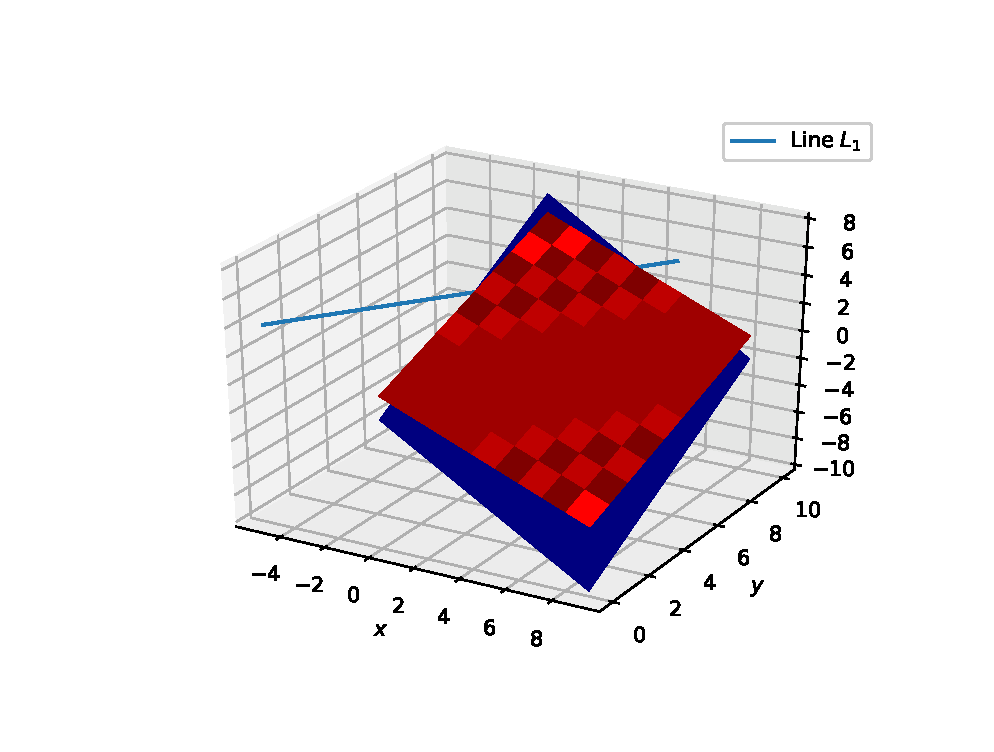
\includegraphics[width=\columnwidth]{./3d/figs/1.1.eps}
\caption{}
\label{fig:1.1}
\end{figure}

\item $L_2$ is the intersection of the planes
\begin{align}
\myvec{1 & 2 & -1}\vec{x} &= 3
\\
\myvec{3 & -1 & 2}\vec{x} &= 1
\end{align}
Show that its equation is
%
\begin{align}
\vec{x} = \frac{1}{7}\myvec{ 5 \\ 8 \\ 0} + \lambda_2 \myvec{ -3 \\ 5 \\ 7}
\label{eq:l2}
\end{align}
\item Plot 
$L_2$.
\\
\solution The following code generates Fig. \ref{fig:1.2}.
\begin{lstlisting}
 
codes/3d/1.2.py
\end{lstlisting}
\begin{figure}[!ht]
\centering
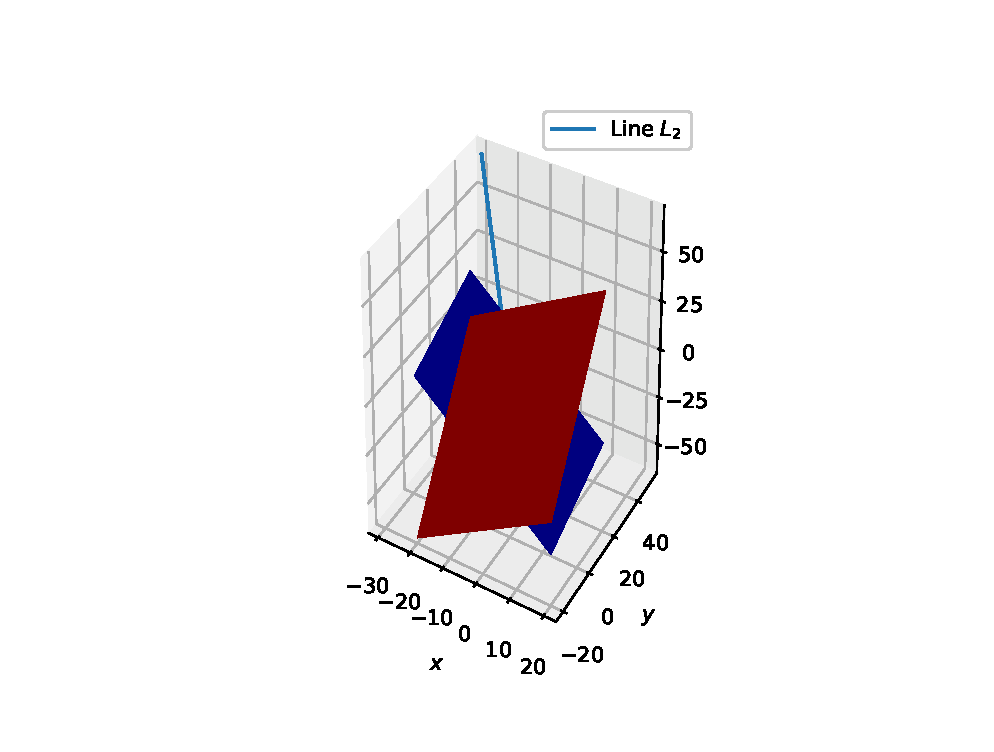
\includegraphics[width=\columnwidth]{./3d/figs/1.2.eps}
\caption{}
\label{fig:1.2}
\end{figure}

\item Do $L_1$ and $L_2$ intersect? If so, find their point of intersection $P$.
\\
\solution From \eqref{eq:l1},\eqref{eq:l2}, the point of intersection is given by
\begin{align}
\label{eq:l1l2pt}
\vec{x} = \frac{1}{7}\myvec{ 5 \\ 8 \\ 0} + \lambda_2 \myvec{ -3 \\ 5 \\ 7} &= \myvec{ 
-5 \\ 0 \\ 4} + \lambda_1 \myvec{ 1 \\ 1 \\ 0}
\\
\implies 
\myvec{1 &  3 \\ 1 & -5 \\ 0 & -7}\vec{\Lambda} &= \frac{1}{7}\myvec{40 \\ 8 \\ -28}
\end{align}
This matrix equation can be solved as
\begin{align}
\myvec{1 &  3 & \frac{40}{7}\\ 1 & -5 &\frac{8}{7}\\ 0 & -7 & -4} &\leftrightarrow \myvec{8 &  0 & 
\frac{224}{7}\\ 0 & 1 &\frac{4}{7}\\ 0 & 1 & \frac{4}{7} }
\\
\leftrightarrow \myvec{1 &  0 & 
4\\ 0 & 1 &\frac{4}{7} } &\implies \vec{\Lambda} = \myvec{4\\\frac{4}{7}}
\end{align}
%
Substituting $\lambda_1 = 4$ in \eqref{eq:l1l2pt}
\begin{align}
\vec{x} = \myvec{4 \\ 4 \\ 0} + \myvec{-5 \\ 0 \\ 4} = \myvec{-1\\ 4\\ 4}
\end{align}
\item Plot $P$.
\\
\solution The following code generates Fig. \ref{fig:1.3}.
\begin{lstlisting}
 
codes/3d/1.3.py
\end{lstlisting}
\begin{figure}[!ht]
\centering
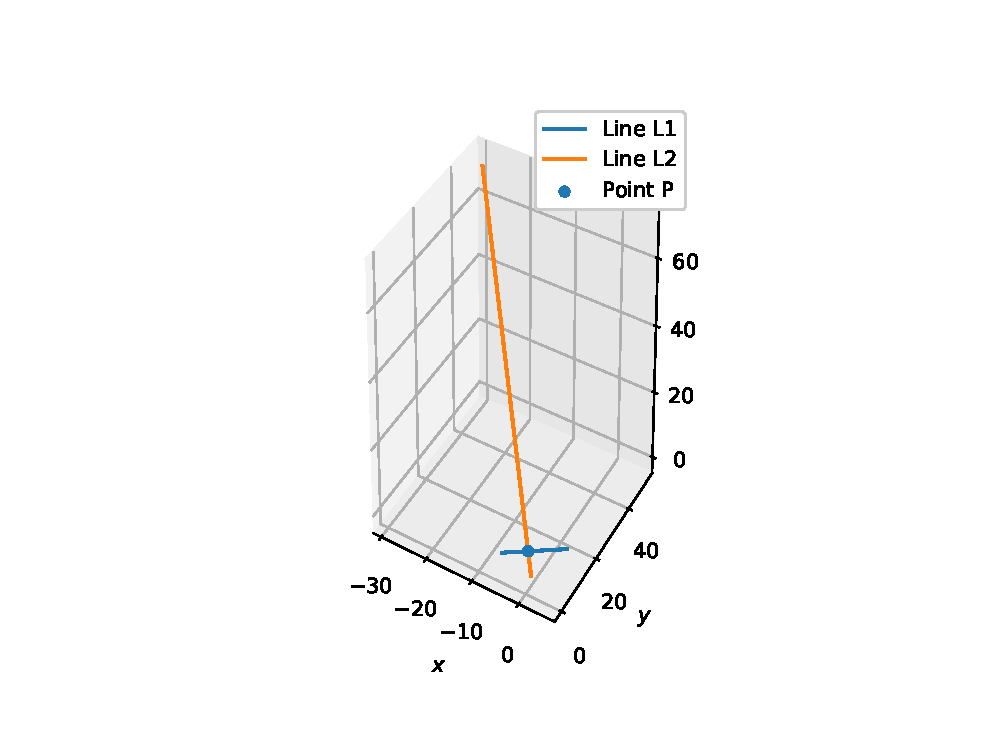
\includegraphics[width=\columnwidth]{./3d/figs/1.3.eps}
\caption{}
\label{fig:1.3}
\end{figure}
\end{enumerate}
 
\subsection{Normal to a Plane}
\renewcommand{\theequation}{\theenumi}
\begin{enumerate}[label=\arabic*.,ref=\thesubsection.\theenumi]
\numberwithin{equation}{enumi}
\item The cross product of $\vec{a},\vec{b}$ is defined as
\begin{equation}
\label{eq:cross}
\vec{a}\times \vec{b} = \myvec{0 & -a_3 & a_2 \\ a_3 & 0 & -a_1 \\ -a_2 & a_1 & 0}\myvec{b_1 \\ b_2 \\ b_3}
\end{equation}
From \eqref{eq:l1}, \eqref{eq:l2}, the direction vectors of $L_1$ and $L_2$ are
\begin{equation}
\myvec{1 \\ 1 \\ 0} \text{ and } \myvec{-3 \\ 5 \\ 7}
\end{equation}
respectively. Find the direction vector of the normal to the plane spanned by $L_1$ and $L_2$.
\\
\solution The desired vector is obtained as
\begin{align}
\myvec{1 \\ 1 \\ 0} \times \myvec{-3 \\ 5 \\ 7} = 
 \myvec{0 & 0 & 1 \\ 0 & 0 & -1 \\ -1 & 1 & 0}\myvec{-3 \\ 5 \\ 7}
= \myvec{7 \\ -7 \\ 8} = \vec{n}
\end{align}
\item Summarize all the above computations through a plot 
\\
\solution The following code generates Fig. \ref{fig:2.1}.
\begin{lstlisting}
codes/3d/2.1.py
\end{lstlisting}
\begin{figure}[!ht]
\centering
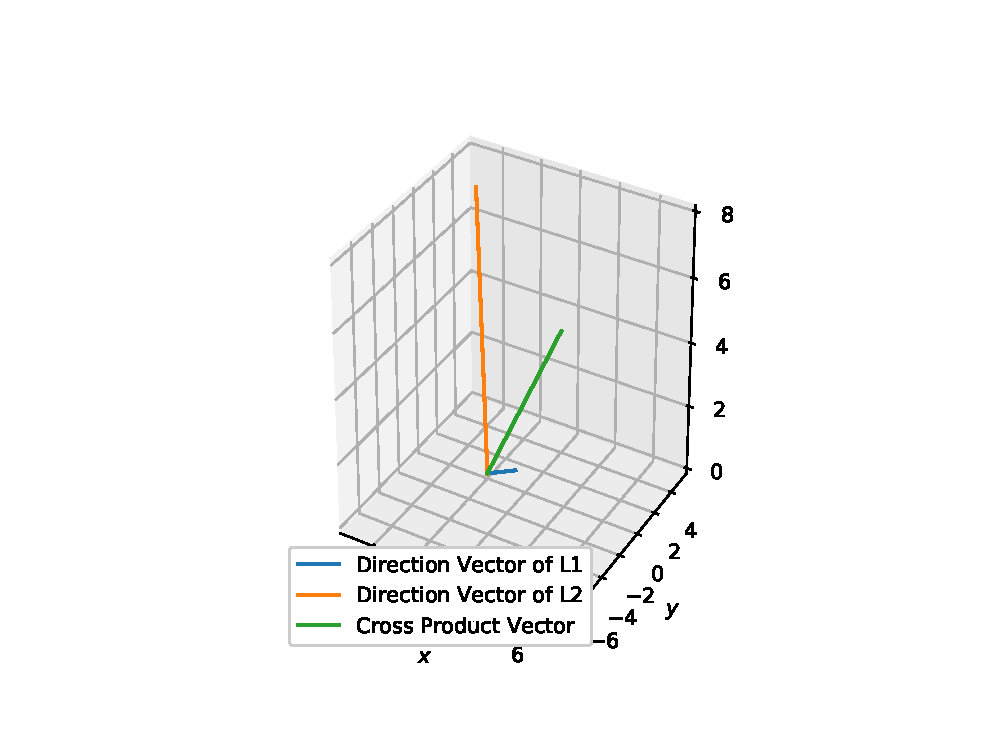
\includegraphics[width=\columnwidth]{./3d/figs/2.1.eps}
\caption{}
\label{fig:2.1}
\end{figure}
\item Find the equation of the plane spanned by $L_1$ and $L_2$.
\\
\solution Let $\vec{x}_0$ be the intersection of $L_1$ and $L_2$.  Then the equation of the plane is
\begin{align}
\brak{\vec{x}-\vec{x}_0}^T\vec{n} &= 0
\\
\implies \vec{x}^T\vec{n} &= \vec{x}_0^T\vec{n}
\\
\implies \vec{x}^T\myvec{7 \\ -7 \\ 8} &= \myvec{-1 & 4 & 4}\myvec{7 \\ -7 \\ 8} =  -3
\end{align}
\item Summarize  the above through a plot. 
\\
\solution The following code generates Fig. \ref{fig:2.2}.
\begin{lstlisting}
 
codes/3d/2.2.py
\end{lstlisting}
\begin{figure}[!ht]
\centering
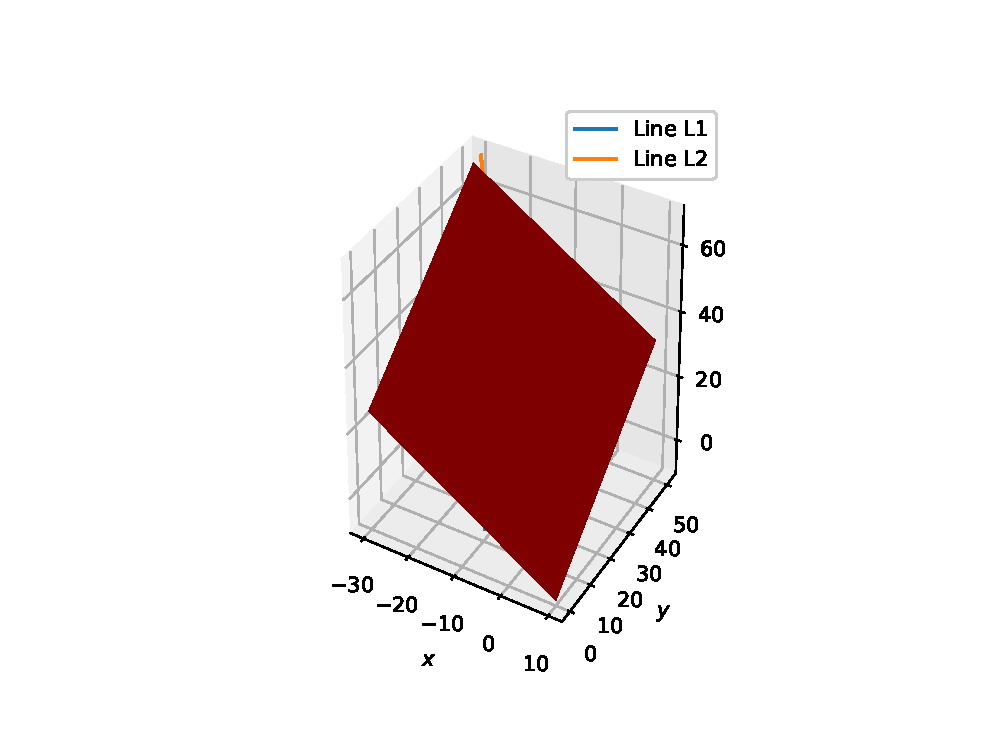
\includegraphics[width=\columnwidth]{./3d/figs/2.2.eps}
\caption{}
\label{fig:2.2}
\end{figure}
\item
Find the distance of the origin from the plane containing the lines $L_1$ and $L_2$.
\\
\solution The distance from the origin to the plane is given by
\begin{equation}
\frac{\abs{\vec{x}_0^T\vec{n}}}{\norm{n}} = \frac{1}{3\sqrt{2}}
\end{equation}
\end{enumerate}
 
\subsection{Projection on a Plane}
\renewcommand{\theequation}{\theenumi}
\begin{enumerate}[label=\arabic*.,ref=\thesubsection.\theenumi]
\numberwithin{equation}{enumi}

%
\item Find the equation of the line $L$ joining the points 
\begin{align}
\vec{A}=\myvec{5 & -1 &4}^T
\\
\vec{B}=\myvec{4 & -1 & 3}^T
\end{align}
\solution The desired equation is
\begin{align}
\vec{x} &= \vec{B} + \lambda\brak{\vec{A}-\vec{B}}
\\
&= \myvec{4 \\ -1 \\ 3} + \lambda \myvec{1 \\ 0 \\ 1}
\label{eq:Lproj}
\end{align}
\item Plot the above line. 
\\
\solution The following code generates Fig. \ref{fig:3.1}.
\begin{lstlisting}
codes/3d/3.1.py
\end{lstlisting}
\begin{figure}[!ht]
\centering
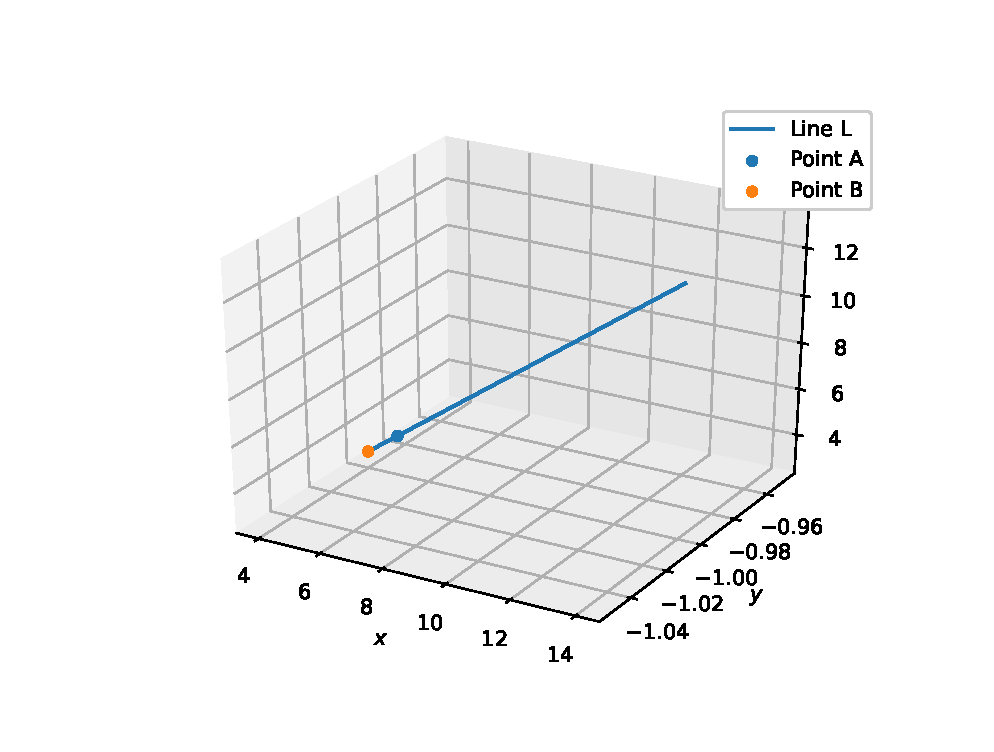
\includegraphics[width=\columnwidth]{./3d/figs/3.1.eps}
\caption{}
\label{fig:3.1}
\end{figure}
\item Find the intersection of $L$ and the plane $P$ given by
\begin{equation}
\myvec{1 & 1 & 1}\vec{x} = 7
\label{eq:Pproj}
\end{equation}
\\
\solution From \eqref{eq:Lproj} and \eqref{eq:Pproj},
\begin{align}
 \myvec{1 & 1 & 1}\myvec{4 \\ -1 \\ 3} + \lambda \myvec{1 & 1 & 1}
\myvec{1 \\ 0 \\ 1} &= 7
\\
\implies 6 + 2\lambda &= 7
\\
\implies \lambda &= \frac{1}{2}
\end{align}
%
Substituting in \eqref{eq:Lproj},
\begin{equation}
\vec{x} = \frac{1}{2}\myvec{9 & -1 & 7}
\end{equation}
\item Sketch the line, plane and the point of intersection.
\\
\solution The following code generates Fig. \ref{fig:3.2}.
\begin{lstlisting}
 
codes/3d/3.2.py
\end{lstlisting}
\begin{figure}[!ht]
\centering
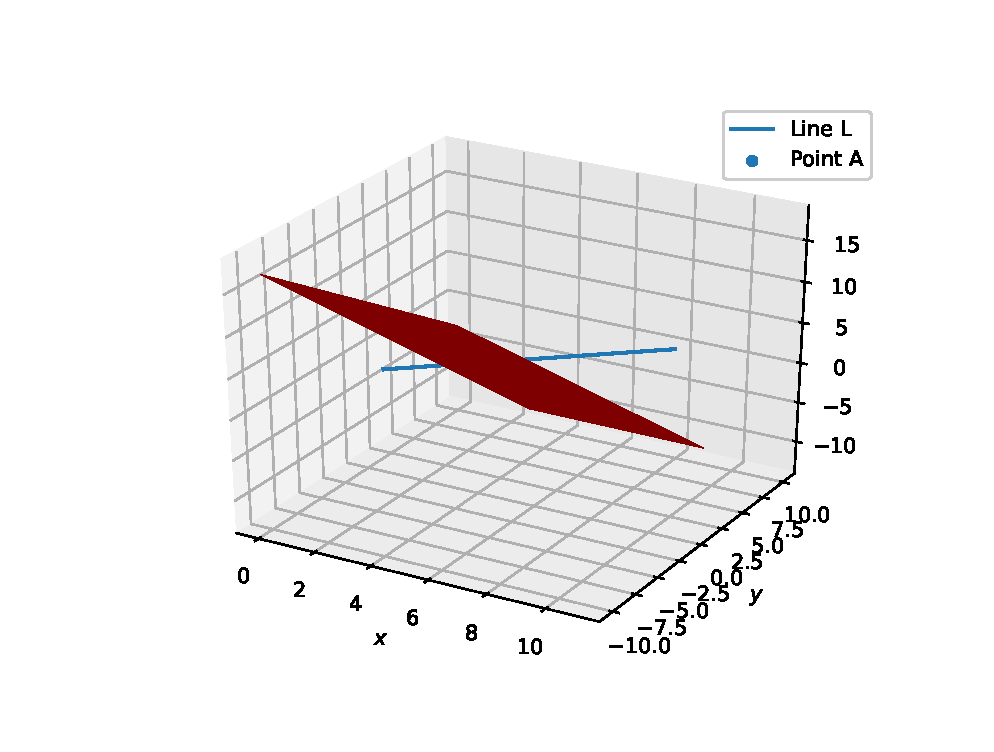
\includegraphics[width=\columnwidth]{./3d/figs/3.2.eps}
\caption{}
\label{fig:3.2}
\end{figure}
\item Find $\vec{C} \in P$  such that $AC \perp P$.  
\\
\solution From \eqref{eq:Pproj}, the direction vector of $AC$ is $\myvec{1 & 1 & 1}^T$.  Hence, the equation of 
$AC$ is
\begin{equation}
\vec{x} = \myvec{5 \\ -1 \\ 4} + \lambda_1  \myvec{1 \\ 1 \\ 1}
\end{equation}
Substituting in \eqref{eq:Pproj}
\begin{align}
 \myvec{1 & 1 & 1}\myvec{5 \\ -1 \\ 4} + \lambda \myvec{1 & 1 & 1}
\myvec{1 \\ 1 \\ 1} &= 7
\\
\implies 8 + 3\lambda_1 &= 7
\\
\implies \lambda_1 &= -\frac{1}{3}
\end{align}
Thus,
\begin{align}
\vec{C} = \frac{1}{3}\myvec{14 \\ -4 \\ 11}
\end{align}
%\item Summarize the above through a plot.
%\\
%\solution The following code generates Fig. \ref{fig:3.3}.
%\begin{lstlisting}
% 
%codes/3d/3.3.py
%\end{lstlisting}
%\begin{figure}[!ht]
%\centering
%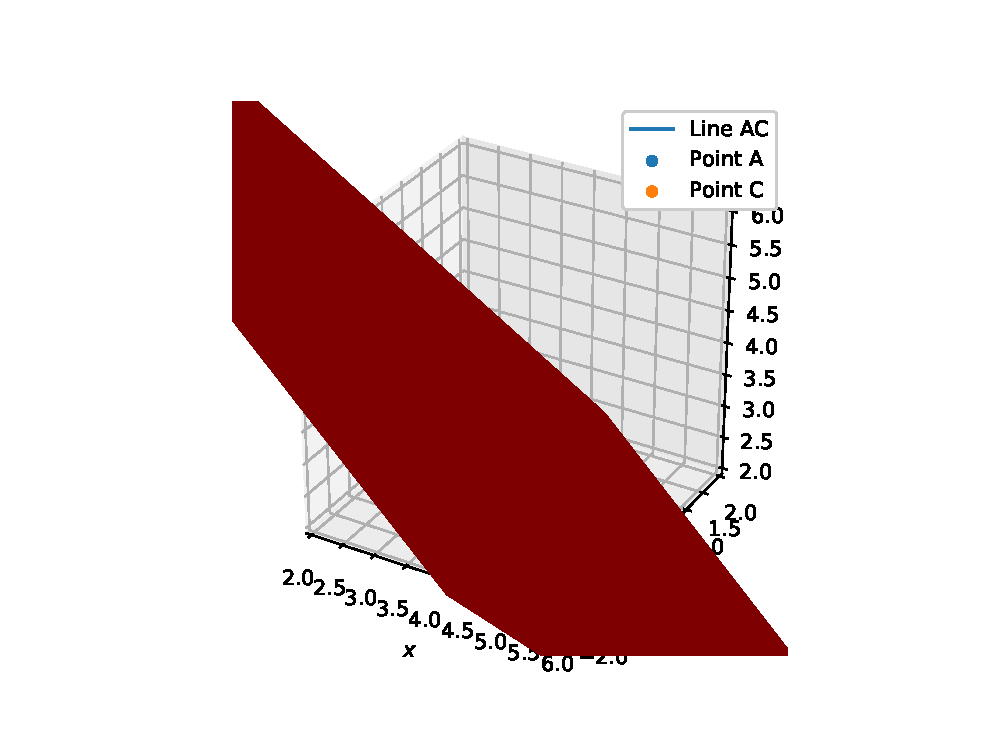
\includegraphics[width=\columnwidth]{./3d/figs/3.3.eps}
%\caption{}
%\label{fig:3.3}
%\end{figure}
\item Show that if $BD \perp P$  such that $\vec{D} \in P$,
\begin{equation}
\vec{D} = \frac{1}{3}\myvec{13 \\ -2 \\ 10}
\end{equation}
%
\item Find the projection of $AB$ on the plane $P$.
\\
\solution The projection is given by
\begin{align}
CD = \norm{\vec{C}-\vec{D}} = \sqrt{\frac{2}{3}}
%\label{eq:homog}
\end{align}
\item Show that the projection of $\vec{x}$ on $\vec{y}$ is
\begin{align}
\label{eq:2019_qp2_14_proj}
\frac{\vec{x}^T\vec{y}}{\norm{\vec{y}}^2}\vec{y}
\end{align}
\end{enumerate}
 
\subsection{Coplanar vectors}
\renewcommand{\theequation}{\theenumi}
\begin{enumerate}[label=\arabic*.,ref=\thesubsection.\theenumi]
\numberwithin{equation}{enumi}
\item If $\vec{u}, \vec{A}, \vec{B}$ are coplanar, show that
\begin{equation}
\vec{u}^T\brak{\vec{A}\times \vec{B}} = 0
\label{eq:coplanar}
\end{equation}
%
\item Find $\vec{A}\times \vec{B}$ given
\begin{align}
\vec{A}=\myvec{2 & 3 & -1}^T
\\
\vec{B}=\myvec{0 & 1 & 1}^T
\end{align}
\solution From \eqref{eq:cross},
\begin{align}
\vec{A}\times \vec{B} &= \myvec{0 & 1& 3 \\ -1 & 0 & -2 \\ -3 & 2 & 0}\myvec{0 \\ 1 \\ 1}
\\
&= \myvec{4 \\ -2 \\ 2}
\label{eq:last_axb}
\end{align}

\item Let $\vec{u}$ be coplanar with $\vec{A}$
%
such that $\vec{u}\perp\vec{A}$ and
\begin{equation}
\vec{u}^T\vec{B} = 24.
\label{eq:uB}
\end{equation}
Find $\norm{\vec{u}}^2$.
\\
\solution From \eqref{eq:last_axb} and the given information,
\begin{align}
\vec{u}^T\myvec{4 & -2 & 2} &=0
\\
\vec{u}^T\myvec{2 & 3 & -1} &=0
\\
\vec{u}^T\myvec{0 & 1 & 1} &=24
\\
\implies \myvec{4 & -2 & 2
\\
2 & 3 & -1
\\
0 & 1 & 1
}\vec{u}
&= \myvec{0 \\ 0 \\ 24}
\\
\implies 
\vec{u} &= 4 \myvec{-1 \\ 2 \\ 4}
\\
\implies \norm{\vec{u}}^2 &= 336
\end{align}
\end{enumerate}
 
\subsection{Orthogonality}
\renewcommand{\theequation}{\theenumi}
\begin{enumerate}[label=\arabic*.,ref=\thesubsection.\theenumi]
\numberwithin{equation}{enumi}

\item Let
\begin{align}
L_1: \quad \vec{x} &= \myvec{1 \\ 0 \\ 0} + \lambda_1 \myvec{-1 \\ 2 \\ 2}
\\
L_2: \quad \vec{x} &=  \lambda_1 \myvec{2 \\-1 \\ 2}
\end{align}
%
Given that  $L_3 \perp L_1, L_3 \perp L_2$, find $L_3$.
\\
\solution Let 
\begin{align}
L_3: \quad \vec{x} &= \vec{c}+ \lambda \vec{m}_3
\end{align}
% 
Then
\begin{align}
\myvec{-1 & 2 & 2
\\
2 &-1 & 2}\vec{m}_3 = \vec{0}
\end{align}
%
Row reducing the coefficient matrix,
\begin{align}
\myvec{-1 & 2 & 2
\\
2 &-1 & 2} &\leftrightarrow 
\myvec{1 & -2 & -2
\\
0 &1 & 2} 
\\
\leftrightarrow 
\myvec{1 & 0 & 2
\\
0 &1 & 2} 
& \implies \vec{m}_3 = \myvec{2 \\ 2 \\ -1}
\end{align}
%
Also, $L_1\perp L_2$, but $L_1 \cup L_2 = \phi$. The given information can be summarized as
\begin{align}
\label{eq:12-given1}
L_1: \quad \vec{x} &= \vec{c}_1 + \lambda_1 \vec{m}_1
\\
L_2: \quad \vec{x} &=  \lambda_2 \vec{m}_2
\\
L_3: \quad \vec{x} &= \vec{c}_3 + \lambda \vec{m}_3
\label{eq:12-given3}
\end{align}
%
where
\begin{align}
\label{eq:12-given12}
\vec{c}_1 = \myvec{1 \\ 0 \\ 0}, \vec{m}_1=  \myvec{-1 \\ 2 \\ 2},
\vec{m}_2 = \myvec{2 \\-1 \\ 2}
\end{align}
The objective is to find $\vec{c}_3$.  Since $L_1 \cup L_3 \ne \phi, L_2 \cup L_3 \ne \phi$, from \eqref{eq:12-given1}-\eqref{eq:12-given3},
\begin{align}
\label{eq:12-isect13}
\vec{c}_1 + \lambda_1 \vec{m}_1 &= \vec{c}_3 + \lambda_3 \vec{m}_3
\\
  \lambda_2 \vec{m}_2 &= \vec{c}_3 + \lambda_4 \vec{m}_3
\label{eq:12-isect23}
\end{align}
%
Using the fact that $L_1\perp L_2\perp L_3$, \eqref{eq:12-isect13}-\eqref{eq:12-isect23} can be expressed as
\begin{align}
%\label{eq:12-isect13}
\vec{m}_1^T\vec{c}_1 + \lambda_1 \norm{\vec{m}}_1^2 &= \vec{m}_1^T\vec{c}_3 
\\
\vec{m}_2^T\vec{c}_1  &= \vec{m}_2^T\vec{c}_3 
\\
\vec{m}_3^T\vec{c}_1  &= \vec{m}_3^T\vec{c}_3 + \lambda_3 \norm{\vec{m}_3}^2
\\
0 &= \vec{m}_1^T\vec{c}_3 
\\
  \lambda_2 \norm{\vec{m}_2}^2 &= \vec{m}_2^T\vec{c}_3 
\\
0 &= \vec{m}_3^T\vec{c}_3  + \lambda_4 \norm{\vec{m}_3}^2
%\label{eq:12-isect23}
\end{align}
%
Simplifying the above, 
\begin{align}
 \lambda_1  &= -\frac{\vec{m}_1^T\vec{c}_1}{\norm{\vec{m}}_1^2} = \frac{1}{9}
\\
 \lambda_2  &= \frac{\vec{m}_2^T\vec{c}_1}{\norm{\vec{m}}_2^2} =\frac{2}{9}
\end{align}
%
Substituting in \eqref{eq:12-isect13} and \eqref{eq:12-isect23},
\begin{align}
L_3: \quad \vec{x} &= \frac{2}{9}\myvec{4 \\ 1 \\ 1} + \lambda_3\myvec{2 \\ 2 \\ -1} \text{ or}
\\
L_3: \quad \vec{x} &= \frac{2}{9}\myvec{2 \\-1 \\ 2} + \lambda_3\myvec{2 \\ 2 \\ -1}
\end{align}
%
The key concept in this question is that orthogonality of $L_1$ and $L_2$ doesnot mean that they intersect.  They are skew lines.
\end{enumerate}
%

 
\subsection{Least Squares}
\renewcommand{\theequation}{\theenumi}
\begin{enumerate}[label=\arabic*.,ref=\thesubsection.\theenumi]
\numberwithin{equation}{enumi}
\item Find the equation of the plane $P$
containing the vectors 
%
\begin{align}
\label{eq:least_vecs}
\vec{x}_1 = \myvec{1 \\ 1 \\ 1}
,
\vec{x}_2 = \myvec{0 \\ 1 \\ 2}
\end{align}
%
\item Show that the vector 
\begin{align}
\vec{y} = \myvec{6 \\ 0 \\ 0}
\end{align}
lies outside $P$.
\item Find the point $\vec{w} \in P$ closest to $\vec{y}$.
\item Show that
\begin{align}
\norm{\vec{y}-\vec{X}\vec{w}}^2 &= \norm{\vec{y}}^2 - \vec{w}^T\vec{X}^T\vec{y} 
\\
& \quad - \vec{y}^TA\vec{w}+\vec{w}^T\vec{X}^T\vec{X}\vec{w}
\end{align}
%
\item Assuming $2\times 2$ matrices and $2 \times 1$ vectors, show that
\begin{align}
\frac{\partial}{\partial\vec{w}}\vec{w}^T\vec{X}^T\vec{y} = \frac{\partial}{\partial\vec{w}}\vec{y}^T\vec{X}\vec{w} = 
\vec{y}^T\vec{X}
\end{align}
\item Show that
\begin{align}
\frac{\partial}{\partial\vec{w}}\vec{w}^T\vec{X}^T\vec{X}\vec{w} = 2\vec{w}^T\brak{\vec{X}^T\vec{X}}
\end{align}
\item Show that 
\begin{align}
\hat{\vec{w}} &= \min_{\vec{w}}\norm{\vec{y}-\vec{X}\vec{w}}^2
\\
 &= \brak{\vec{X}^T\vec{X}}^{-1}\vec{X}^T \vec{y}
\label{eq:least_sol}
\end{align}
\item Let 
\begin{align}
\vec{X} = \myvec{\vec{x}_1 & \vec{x}_2}.
\end{align}
from \eqref{eq:least_vecs}.
Verify \eqref{eq:least_sol}.
\item
Run the following Python code and comment on the output for different values of $\mbf{x}$
\begin{lstlisting}
 
codes/matrix/Prob1_4.py
\end{lstlisting}
%	\begin{verbatim}
%%Code written by GVV Sharma March 30, 2016
%%Released under GNU GPL.  Free to use for anything.
%
%%This program compares the norm defined for the least-squares solution
%%for the correct solution vs other data points.
%%You will find that the metric is the smallest for the correct value.
%
%clear;
%close;
%
%A = [1 0; 1 1; 1 2]; %The input matrix
%b = [6;0;0]; %The output vector
%
%P = inv(A'*A)*A';%pseudoinverse
%
%x_ls = P*b; %The least squares solution
%
%x = [5;-5]; %Any random input
%
%exact_ls_metric = norm(b-A*x_ls)^2 %The metric for actual soltuion
%random_ls_metric = norm(b-A*x)^2 %metric for a random value of x
%	
%	\end{verbatim}


%
%\item
%	Type the following code in Python and observe the output.
%\begin{verbatim}
%%Code written by GVV Sharma March 31, 2016
%%Released under GNU GPL.  Free to use for anything.
%
%
%%This program plots the least squares metric for a range of
%%vectors x in the mesh with vertices (-10,-10),(-10,10),(10,-10)
%%%and (10,10)
%
%%The result is a 3-D mesh.  The theoretical minimum is (5,-3)
%%Values obtained through the following program are close to the 
%%theoreticl solution
%
%
%clear;
%close;
%
%A = [1 0; 1 1; 1 2]; %The input matrix
%b = [6;0;0]; %The output vector
%
%
%x1 = linspace(-10,10,50); %generating points in x-axis
%x2 = linspace(-10,10,50);  %generating points in y-axis
%
%[xx, yy] = meshgrid(x1,x2);
%
%ffun = @(x,y) norm(b-A*[x;y])^2;
%
%f = arrayfun(ffun,xx,yy);
%
%mesh(xx,yy,f)
%
%[M I] = min(f(:)); %vectorize the 50 x 50 matrix f, find min
%%M = min value , I is the index of the f_min
%
%[I_r I_c] = ind2sub(size(f),I); %Get the row, col index of f_min
%
%
%%The least square solution
%xx(I_r,I_c) 
%yy(I_r,I_c)
%%The minimum value of metric
%M
%
%\end{verbatim}
%
%
\item
	Compare the results obtained by typing the following code with the results in the previous problem.
\begin{lstlisting}
 
codes/matrix/Prob1_6.py
\end{lstlisting}
%\begin{verbatim}
%Code written by GVV Sharma March 31, 2016
%Released under GNU GPL.  Free to use for anything.


%This program finds the theoretical least squares solution using 
%SVD 

%clear;
%close;
%
%A = [1 0; 1 1; 1 2]; %The input matrix
%b = [6;0;0]; %The output vector
%
%
%[U S V] = svd(A); % Computing the SVD of A
%
%temp_S = 1./diag(S); %inverting the diagonal values of S
%
%Splus = [diag(temp_S) zeros(2,1)]; %inverse transpose of S
%
%Aplus = V*Splus*U'; %The Moore-Penrose pseudo-inverse
%
%Aplus*b %least squares solution.
%
%\end{verbatim}

%
\item
	Type the following code in Python and run.  Comment.

%
\begin{lstlisting}
 
codes/matrix/Prob1_7.py
\end{lstlisting}
\end{enumerate}

 
\subsection{Singular Value Decomposition}
\renewcommand{\theequation}{\theenumi}
\begin{enumerate}[label=\arabic*.,ref=\thesubsection.\theenumi]
\numberwithin{equation}{enumi}
\item Let $\mbf{v}_1,\mbf{v}_2$ be the columns of $\mbf{C} = \vec{X}^T\vec{X}$.

\item
	Obtain $\mbf{u}_1,\mbf{u}_2$ from $\mbf{v}_1,\mbf{v}_2$ through the following equations. 
	%
\begin{align}
\mbf{u}_1&= \frac{\mbf{v}_1}{\norm{\mbf{v}_1}}
\\
\hat{\mbf{u}}_2 &= \mbf{v}_2 - \brak{\mbf{v}_2,\mbf{u}_1}\mbf{u}_1
\\
\mbf{u}_2 &= \frac{\hat{\mbf{u}}_2}{\norm{\hat{\mbf{u}}_2}}
\end{align}
	%
	This procedure is known as Gram-Schmidt orthogonalization.


\item
Stack the vectors $\mbf{u}_1,\mbf{u}_2$ in columns to obtain the matrix $\mbf{Q}$.  Show that $\mbf{Q}$ is orthogonal.  


\item
	From the Gram-Schmidt process, show that $\mbf{C}=\mbf{Q}\mbf{R}$, where $\mbf{R}$ is an upper triangular matrix.  This is known as the $\mbf{Q}-\mbf{R}$ decomposition.  


\item
	Find an orthonormal basis for $\vec{X}^T\vec{X}$ comprising of the eigenvectors.  Stack these orthonormal eigenvectors in a matrix $\mbf{V}$. This is known as {\em Orthogonal Diagonalization}.  

\item
	Find the singular values of $\vec{X}^T\vec{X}$.  The singular values are obtained by taking the square roots of its eigenvalues.  

\item
	Stack the singular values of $\vec{X}^T\vec{X}$ diagonally to obtain a matrix $\mbf{\Sigma}$.


\item
	Obtain the matrix $\vec{X}\mbf{V}$.  Verify if the columns of this matrix are orthogonal.


\item
	Extend the columns of $\vec{X}\mbf{V}$ if necessary, to obtain an orthogonal matrix $\mbf{U}$.


\item
	Find $\mbf{U}\mbf{\Sigma}\mbf{V}^T$.  Comment.


\end{enumerate}

 
\subsection{JEE Exercises}
\renewcommand{\theequation}{\theenumi}
\begin{enumerate}[label=\arabic*.,ref=\thesubsection.\theenumi]
\numberwithin{equation}{enumi}

\item Let $\overrightarrow{A}$, $\overrightarrow{B}$, $\overrightarrow{C}$ be vectors of length 3, 4, 5 respectively. Let $\overrightarrow{A}$ be perpendicular to $\overrightarrow{B}$ + $\overrightarrow{C}$, $\overrightarrow{B}$ to 
$\overrightarrow{C}$ + $\overrightarrow{A}$ and $\overrightarrow{C}$ to $\overrightarrow{A}$ + $\overrightarrow{B}$. Then the length of vector $\overrightarrow{A}$ + $\overrightarrow{B}$ + $\overrightarrow{C}$ is..............

\item The unit vector perpendicular to the plane determined by P(1, -1, 2), Q(2, 0, -1) and R(0, 2, 1) is.........

\item The area of the triangle whose vertices are  A(1, -1, 2), B(2, 1, -1) and C(3, -1, 2) is........

\item A, B, C, and D are four points in a plane with position vectors a, b, c, and d respectively such that
\begin{align*}
(\overrightarrow{a} - \overrightarrow{d}) (\overrightarrow{b} - \overrightarrow{c}) 
= (\overrightarrow{b} - \overrightarrow{d}) (\overrightarrow{c} - \overrightarrow{a}) = 0
\end{align*}
The Point D, then is the.................of the triangle ABC.

\item If 
$\begin{vmatrix}
a & a^{2} & 1 + a^{3} \\ b & b^{2} & 1 + b^{3} \\ c & c^{2} & 1 + c^{3} 
\end{vmatrix} = 0$ 
and the vectors 
\begin{align*}
\overrightarrow{A} = (1, a, a^{2}), \overrightarrow{B} = (1, b, b^{2}), \overrightarrow{C} = (1, c, c^{2})
\end{align*}
are non-olar, then the product abc = ............

\item If $\overrightarrow{A}$  $\overrightarrow{B}$  $\overrightarrow{C}$ are three non-polar vectors, then 
\begin{align*}
\frac{\overrightarrow{A} . \overrightarrow{B} \times \overrightarrow{C}}{\overrightarrow{C} \times \overrightarrow{A} . \overrightarrow{B}} + \frac{\overrightarrow{B} . \overrightarrow{A} \times \overrightarrow{C}}{\overrightarrow{C} . \overrightarrow{A} \times \overrightarrow{B}} = ..............
\end{align*}

\item If $\overrightarrow{A}$ = (1, 1, 1), $\overrightarrow{C}$ = (0, 1, -1) are given vectors, then a vector B satisfying the equations $\overrightarrow{A} \times \overrightarrow{B} = \overrightarrow{C}$ and 
$\overrightarrow{A} . \overrightarrow{B}$ = 3.............

\item If the vectors a$\hat{i}$ + $\hat{j}$ + $\hat{k}$, $\hat{i}$ + b$\hat{j}$ + $\hat{j}$, $\hat{i}$ + $\hat{j}$ + c$\hat{k}$ $(a \neq b \neq c \neq 1)$ are co-planar, then the value of 
\begin{align*}
\frac{1}{1 - a} + \frac{1}{1 - b} + \frac{1}{1 - c} = ..........
\end{align*}

\item Let b = 4$\hat{i}$ + 3$\hat{j}$ and $\overrightarrow{c}$ be two vectors perpendicular to each other in the xy - plane. All vectors in the same plane having projections 1 and 2 along $\overrightarrow{b}$ and $\overrightarrow{c}$, respectively are given by..........

\item The components of a vector $\overrightarrow{a}$ along and perpendicular to a non-zero vector 
$\overrightarrow{b}$ are............. and .............respectively.

\item Given that $\overrightarrow{a}$ = (1, 1, 1), $\overrightarrow{c}$ = (0, 1, -1), $\overrightarrow{a}\overrightarrow{b}$ = 3 and $\overrightarrow{a} \times \overrightarrow{b} = \overrightarrow{c}$, then $\overrightarrow{b}$ = .................

\item A unit vector co-planr with $\overrightarrow{i} + \overrightarrow{j} + 2\overrightarrow{k}$ and 
$\overrightarrow{i} + 2\overrightarrow{j} + \overrightarrow{k}$ and perpendicular to $\overrightarrow{i} + \overrightarrow{j} + \overrightarrow{k}$ is............

\item A unit vector perpendicular to the plane determined by the points P(1, -1, 2), Q(2, 0, -1) and R(0, 2, 1) is..........

\item A non-zero vector $\overrightarrow{a}$ is parallel to the line of intersection of the plane determined by the vectors $\hat{i}$, $\hat{i}$ + $\hat{j}$ and plane determined by the vectors $\hat{i}$ - $\hat{j}$, 
$\hat{i}$ + $\hat{k}$. The angle between $\overrightarrow{a}$ and the vector $\hat{i}$ - 2$\hat{j}$ + 2$\hat{k}$ is...........

\item If $\overrightarrow{b}$ and $\overrightarrow{c}$ are any two non-collinear unit vectors and $\overrightarrow{a}$ is any vector 
\begin{align*}
(\overrightarrow{a} . \overrightarrow{b})\overrightarrow{b} + (\overrightarrow{a} . \overrightarrow{c})\overrightarrow{c} + \frac{\overrightarrow{a} . (\overrightarrow{b} \times \overrightarrow{c})}{\begin{vmatrix} \overrightarrow{b} \times \overrightarrow{c} \end{vmatrix}} (\overrightarrow{b} \times \overrightarrow{c}) =
\end{align*}

\item Let OA = a, OB = 10a + 2b and OC = b where O, A, and C are non-collinear points. Let p denote thea area of the quadrilateral OABC, and let q denote the area of the parallelgram with OA and OC as adjacent sides. If p = kq, then k = ............

\textbf{(B). True/False}

\item Let $\overrightarrow{A}$, $\overrightarrow{B}$ and $\overrightarrow{C}$ be unit vectors suppose that $\overrightarrow{A}.\overrightarrow{B}$ = $\overrightarrow{A}.\overrightarrow{C}$ = 0, and the angle between $\overrightarrow{B}$ and $\overrightarrow{C}$ is $\frac{\pi}{6}$. Then $\overrightarrow{A}$ = $\pm 2(\overrightarrow{B} \times \overrightarrow{C})$.

\item If X.A = 0, X.B = 0, X.C = 0 for some non-zero vector X, then [A B C] = 0.

\item The points with position vectors a + b, a - b, and a + kb are collinear for all real values of k.

\item For any three vectors $\overrightarrow{a}$, $\overrightarrow{b}$ and $\overrightarrow{c}$, 
\begin{align*}
(\overrightarrow{a}  \overrightarrow{b}) . (\overrightarrow{b} - \overrightarrow{c}) \times (\overrightarrow{c} - \overrightarrow{a}) = 2\overrightarrow{a} . (\overrightarrow{b} \times \overrightarrow{c})
\end{align*}

\textbf{(C). MCQs with One Correct Answer}
\item The scalar $\overrightarrow{A} . (\overrightarrow{B} + \overrightarrow{C}) \times (\overrightarrow{A} + \overrightarrow{B} + \overrightarrow{C})$ equals:
\begin{enumerate}
\item 0
\item $[\overrightarrow{A}  \overrightarrow{B}  \overrightarrow{C}] + [\overrightarrow{B} \overrightarrow{C} \overrightarrow{A}]$
\item $[\overrightarrow{A} \overrightarrow{B} \overrightarrow{C}]$
\item None of these
\end{enumerate}

\item For non-zero vectors $\overrightarrow{a}$, $\overrightarrow{b}$, $\overrightarrow{c}$, $| (\overrightarrow{a} \times \overrightarrow{b}) .  \overrightarrow{c} |$ = $|\overrightarrow{a}||\overrightarrow{b}||\overrightarrow{c}|$ holds if and only if 
\begin{enumerate}
\item $\overrightarrow{a}.\overrightarrow{b} = 0$, $\overrightarrow{b}.\overrightarrow{c} = 0$
\item $\overrightarrow{b}.\overrightarrow{c} = 0$, $\overrightarrow{c}.\overrightarrow{a} = 0$
\item $\overrightarrow{c}.\overrightarrow{a} = 0$, $\overrightarrow{a}.\overrightarrow{b} = 0$
\item $\overrightarrow{a}.\overrightarrow{b}$ = $\overrightarrow{b}.\overrightarrow{c}$  = $\overrightarrow{c}.\overrightarrow{a}$ = 0
\end{enumerate}

\item The volume of the parallelopiped whose sides are given by $\overrightarrow{OA}$ = 2i - 2j, $\overrightarrow{OB}$ = i + j - k, $\overrightarrow{OC}$ = 3i - k, is
\begin{enumerate}
\item $\frac{4}{13}$
\item 4
\item $\frac{2}{7}$
\item None of these
\end{enumerate}

\item The points with position vectors 60i + 3j, 40i - 8j, ai - 52j are collinear if
\begin{enumerate}
\item a = -40
\item a = 40
\item a = 20
\item None of these
\end{enumerate}

\item Let $\overrightarrow{a}$, $\overrightarrow{b}$, $\overrightarrow{c}$ be three non-coplanar vectors and $\overrightarrow{p}$, $\overrightarrow{q}$, $\overrightarrow{r}$, are vectors defined by the relations 
\begin{align*}
\overrightarrow{p} = \frac{\overrightarrow{b} \times \overrightarrow{c}}{[\overrightarrow{a}\overrightarrow{b}\overrightarrow{c}]}, \overrightarrow{q} = \frac{\overrightarrow{c} \times \overrightarrow{a}}{[\overrightarrow{a}\overrightarrow{b}\overrightarrow{c}]}, \overrightarrow{r} = \frac{\overrightarrow{a} \times \overrightarrow{b}}{[\overrightarrow{a}\overrightarrow{b}\overrightarrow{c}]}
\end{align*}
then the value of the expression $(\overrightarrow{a} + \overrightarrow{b}).\overrightarrow{p}$ + $(\overrightarrow{b} + \overrightarrow{c}).\overrightarrow{q}$ + $(\overrightarrow{c} + \overrightarrow{a}).\overrightarrow{r}$ is eqaul to
\begin{enumerate}
\item 0
\item 1
\item 2
\item 3
\end{enumerate}

\item Let a, b, c be distinct non-negative numbers. If the vectors a$\hat{i}$ + a$\hat{j}$ + c$\hat{k}$, 
$\hat{i}$ + $\hat{k}$ and c$\hat{i}$ + c$\hat{j}$ + b$\hat{k}$ lie in a plane, then c is
\begin{enumerate}
\item the arithmetic mean of a and b
\item the geomemetic mean of a and b
\item the harmonic mean of a and b
\item equal to zero
\end{enumerate}

\item Let $\overrightarrow{p}$ and $\overrightarrow{q}$ be the position vectors of P and Q respectively, with respect to O $|\overrightarrow{p}|$ = p, $|\overrightarrow{q}|$ = q. The points R and S divide PQ internally and externally in the ratio 2:3 respectively. If OR and OS are perpendicular then
\begin{enumerate}
\item $9q^{2} = 4q^{2}$
\item $4p^{2} = 9q^{2}$
\item 9p = 4q
\item 4p = 9q
\end{enumerate}

\item Let $\alpha$, $\beta$, $\gamma$ be distinct real numbers. The points with postion vectors 
\begin{align*}
\alpha \hat{i} + \beta \hat{j} + \gamma \hat{k}, \beta \hat{i} + \gamma \hat{j} + \alpha \hat{k}, 
\gamma \hat{i} + \alpha \hat{j} + \beta \hat{k}
\end{align*}
\begin{enumerate}
\item are collinear
\item form an equilateral triangle
\item form an scalene triangle
\item form a right angled triangle
\end{enumerate}

\item Let $\overrightarrow{a}$ = $\hat{i}$ - $\hat{j}$, $\overrightarrow{b}$ = $\hat{j}$ - $\hat{k}$, 
$\overrightarrow{c}$ = $\hat{k}$ - $\hat{i}$. If $\overrightarrow{d}$ is a unit vector such that 
$\overrightarrow{a}$ . $\overrightarrow{d}$ = 0 = $[\overrightarrow{b} \overrightarrow{c} \overrightarrow{d}]$, then $\overrightarrow{d}$ equals
\begin{enumerate}
\item $\pm$ $\frac{\hat{i} + \hat{j} - 2\hat{k}}{\sqrt{6}}$
\item $\pm$ $\frac{\hat{i} + \hat{j} - \hat{k}}{\sqrt{3}}$
\item $\pm$ $\frac{\hat{i} + \hat{j} + 2\hat{k}}{\sqrt{3}}$
\item $\pm \hat{k}$
\end{enumerate}

\item If $\overrightarrow{a}$, $\overrightarrow{b}$, $\overrightarrow{c}$ are non coplanar vectors such that 
\begin{align*}
\overrightarrow{a} \times (\overrightarrow{b} \times \overrightarrow{c}) = \frac{(\overrightarrow{b} + \overrightarrow{c})}{\sqrt{2}}
\end{align*}
then the angle between $\overrightarrow{a}$ and $\overrightarrow{b}$ is
\begin{enumerate}
\item $\frac{3\pi}{4}$
\item $\frac{\pi}{4}$
\item $\frac{\pi}{2}$
\item $\pi$
\end{enumerate}

\item Let $\overrightarrow{u}$, $\overrightarrow{v}$ and $\overrightarrow{w}$ be vectors such that $\overrightarrow{u}$ + $\overrightarrow{v}$ + $\overrightarrow{w}$ = 0. If $|\overrightarrow{u}|$ = 3, $|\overrightarrow{v}|$ = 4, $|\overrightarrow{w}|$ = 5, then $\overrightarrow{u}.\overrightarrow{v}$  + $\overrightarrow{v}.\overrightarrow{w}$ + $\overrightarrow{w}.\overrightarrow{u}$ is
\begin{enumerate}
\item 47
\item -25
\item 0
\item 25
\end{enumerate}

\item If $\overrightarrow{a}$, $\overrightarrow{b}$ and $\overrightarrow{c}$ are three non polar vectors, then $\overrightarrow{a}$ + $\overrightarrow{b}$ + $\overrightarrow{c}$ . [($\overrightarrow{a}$ + $\overrightarrow{b})$ $\times$ ($\overrightarrow{a}$ + $\overrightarrow{c})$] equals
\begin{enumerate}
\item 0
\item 1[$\overrightarrow{a}$  $\overrightarrow{b}$  $\overrightarrow{c}$]
\item 2[$\overrightarrow{a}$  $\overrightarrow{b}$  $\overrightarrow{c}$]
\item - [$\overrightarrow{a}$  $\overrightarrow{b}$  $\overrightarrow{c}$]
\end{enumerate}

\item Let a = 2i + j - 2k and b = i + j. If c is a vector such that a.c = $|c|$, $|c - a|$ = 2$\sqrt{2}$ and the angle between $(a \times b)$ and c is $30^{\degree}$, then $| (a \times b) \times c| $ = 
\begin{enumerate}
\item $\frac{2}{3}$
\item $\frac{3}{2}$
\item 2
\item 3
\end{enumerate}

\item a = 2i + j + k, b = i + 2j - k and a unit vector c be coplanar. If c is perpendicular to a, then c = 
\begin{enumerate}
\item $\frac{1}{\sqrt{2}}$(-j + k)
\item $\frac{1}{\sqrt{3}}$(-i - j - k)
\item $\frac{1}{\sqrt{5}}$(i - 2j)
\item $\frac{1}{\sqrt{3}}$(i - j - k)
\end{enumerate}

\item If the vectors $\overrightarrow{a}$, $\overrightarrow{b}$ and $\overrightarrow{c}$ form the sides BC, CA, AB respectively of a triangle ABC, then
\begin{enumerate}
\item $\overrightarrow{a} . \overrightarrow{b}$ + $\overrightarrow{b} . \overrightarrow{c}$ + $\overrightarrow{c} . \overrightarrow{a}$ = 0
\item $\overrightarrow{a} \times \overrightarrow{b}$ = $\overrightarrow{b} \times \overrightarrow{c}$ = $\overrightarrow{c} \times \overrightarrow{a}$
\item $\overrightarrow{a} . \overrightarrow{b}$ = $\overrightarrow{b} . \overrightarrow{c}$ = $\overrightarrow{c} . \overrightarrow{a}$ = 0
\item $\overrightarrow{a} \times \overrightarrow{b}$ + $\overrightarrow{b} \times \overrightarrow{c}$ + $\overrightarrow{c} \times \overrightarrow{a}$ = 0
\end{enumerate}

\item Let the vectors $\overrightarrow{a}$, $\overrightarrow{b}$, $\overrightarrow{c}$ and 
$\overrightarrow{d}$ be such that 
\begin{align*}
(\overrightarrow{a} \times \overrightarrow{b}) \times (\overrightarrow{c} \times \overrightarrow{d}) = 0.
\end{align*}
Let $P_1$ and $P_2$ be planes determined by the pairs of the vectors $\overrightarrow{a}$, $\overrightarrow{b}$ and $\overrightarrow{c}$, $\overrightarrow{d}$ respectively. Then the angle between $P_1$ and $P_2$ is
\begin{enumerate}
\item 0
\item $\frac{\pi}{4}$
\item $\frac{\pi}{3}$
\item $\frac{\pi}{2}$
\end{enumerate}

\item If $\overrightarrow{a}$, $\overrightarrow{b}$ and $\overrightarrow{c}$ are unit co-planar vectors, then the scalar triple product [2$\overrightarrow{a}$ - $\overrightarrow{b}$, 2$\overrightarrow{b}$ - $\overrightarrow{c}$, 2$\overrightarrow{c}$ - $\overrightarrow{a}$] = 
\begin{enumerate}
\item 0
\item 1
\item -$\sqrt{3}$
\item $\sqrt{3}$
\end{enumerate}

\item Let 
\begin{align*}
\overrightarrow{a} = \overrightarrow{i} - \overrightarrow{k}
\end{align*}
\begin{align*}
\overrightarrow{b} = x\overrightarrow{i} + \overrightarrow{j} + (1 - x)\overrightarrow{k}
\end{align*}
\begin{align*}
\overrightarrow{c} = y\overrightarrow{i} + x\overrightarrow{j} + (1 + x -y)\overrightarrow{k}
\end{align*}
Then $[\overrightarrow{a}\overrightarrow{b}\overrightarrow{c}]$ depends on
\begin{enumerate}
\item only x
\item only y
\item Neither x nor y
\item both x and y
\end{enumerate}

\item If $\overrightarrow{a}$, $\overrightarrow{b}$ and $\overrightarrow{c}$ are unit vectors, then 
\begin{align*}
|\overrightarrow{a} - \overrightarrow{b}|^{2} + |\overrightarrow{b} - \overrightarrow{c}|^{2} + |\overrightarrow{c} - \overrightarrow{a}|^{2}
\end{align*}
does not exceed.
\begin{enumerate}
\item 4
\item 9
\item 8
\item 6
\end{enumerate}

\item If $\overrightarrow{a}$ and $\overrightarrow{b}$ are two unit vectors such that $\overrightarrow{a}$ + 2$\overrightarrow{b}$ and 5$\overrightarrow{a}$ - 4$\overrightarrow{b}$ are perpendicular to each other then the angle between $\overrightarrow{a}$ and $\overrightarrow{b}$ is
\begin{enumerate}
\item $45^{\degree}$
\item $60^{\degree}$
\item $\cos^{-1}(\frac{1}{3})$
\item $\cos^{-1}(\frac{2}{7})$
\end{enumerate}

\item Let $\overrightarrow{V}$ = 2$\overrightarrow{i}$ + $\overrightarrow{j}$ - $\overrightarrow{k}$ and $\overrightarrow{W}$ = $\overrightarrow{i}$ + 3$\overrightarrow{k}$. If $\overrightarrow{U}$ is a unit vector, then the maximum value of the scalar triple product $|\overrightarrow{U}\overrightarrow{V}\overrightarrow{W}|$
is
\begin{enumerate}
\item -1
\item $\sqrt{10}$ + $\sqrt{6}$
\item $\sqrt{59}$
\item $\sqrt{60}$ 
\end{enumerate}

\item The value of k such that 
\begin{align*}
\frac{x - 4}{1} = \frac{y - 2}{1} = \frac{z - k}{2}
\end{align*}
lies in the plane 2x - 4y + z = 7, is
\begin{enumerate}
\item 7
\item -7
\item no real value
\item 4
\end{enumerate}

\item The value of $'a'$ so that the volume of parallelopiped formed by $\overrightarrow{i}$ + a$\overrightarrow{j}$ + $\overrightarrow{k}$, $\overrightarrow{j}$ + a$\overrightarrow{k}$ and a$\overrightarrow{i}$ + $\overrightarrow{k}$ becomes minimum is
\begin{enumerate}
\item -3
\item 3
\item $\frac{1}{\sqrt{3}}$
\item $\sqrt{3}$
\end{enumerate}

\item If $\overrightarrow{a}$ = $(\overrightarrow{i} + \overrightarrow{j} + \overrightarrow{k})$, $\overrightarrow{a}$ . $\overrightarrow{b}$ = 1 and $\overrightarrow{a} \times \overrightarrow{b}$ = 
$\overrightarrow{j}$ - $\overrightarrow{k}$, then $\overrightarrow{b}$ is
\begin{enumerate}
\item $\overrightarrow{i} - \overrightarrow{j} + \overrightarrow{k}$
\item 2$\overrightarrow{j} - \overrightarrow{k}$
\item $\overrightarrow{i}$
\item 2$\overrightarrow{i}$
\end{enumerate}

\item If the lines 
\begin{align*}
\frac{x - 1}{2} = \frac{y + 1}{3} = \frac{z - 1}{4}
\end{align*}
\begin{align*}
\frac{x - 3}{1} = \frac{y - k}{2} = \frac{z}{1}
\end{align*}
intersect, then the value of k is
\begin{enumerate}
\item 3/2
\item 9/2
\item -2/9
\item -3/2
\end{enumerate}

\item The unit vector which is orthogonal to the vector 3$\overrightarrow{i}$ + 2$\overrightarrow{j}$ + $\overrightarrow{k}$ and is co-planar with the vectors 2$\overrightarrow{i}$ + $\overrightarrow{j}$ + $\overrightarrow{k}$ and $\overrightarrow{i}$ - $\overrightarrow{j}$ + $\overrightarrow{k}$ is
\begin{enumerate}
\item $\frac{2\overrightarrow{i} - 6\overrightarrow{j} + \overrightarrow{k}}{\sqrt{41}}$
\item $\frac{2\overrightarrow{i} - 3\overrightarrow{j}}{\sqrt{13}}$
\item $\frac{3\overrightarrow{i} - \overrightarrow{k}}{10}$
\item $\frac{4\overrightarrow{i} + 3\overrightarrow{j} - 3\overrightarrow{k}}{34}$
\end{enumerate}

\item A variable plane at a distance of the one unit from the origin cuts the coordinates axes at A, B, and C. If the centroid D(x, y, z) of triangle ABC satisfies the relation
\begin{align*}
\frac{1}{x^{2}} + \frac{1}{y^{2}} + \frac{1}{z^{2}} = k
\end{align*}
then the value of k is
\begin{enumerate}
\item 3
\item 1
\item $\frac{1}{3}$
\item 9
\end{enumerate}

\item If $\overrightarrow{a}$, $\overrightarrow{b}$, $\overrightarrow{c}$ are three non-zero, non-polar vectors and 
\begin{align*}
\overrightarrow{b_1} = \overrightarrow{b} - \frac{\overrightarrow{b}.\overrightarrow{a}}{|\overrightarrow{a}|^{2}}\overrightarrow{a},
\end{align*}
\begin{align*}
\overrightarrow{b_2} = \overrightarrow{b} + \frac{\overrightarrow{b}.\overrightarrow{a}}{|\overrightarrow{a}|^{2}}\overrightarrow{a} 
\end{align*}
\begin{align*}
\overrightarrow{c_1} = \overrightarrow{c} - \frac{\overrightarrow{c}.\overrightarrow{a}}{|\overrightarrow{a}|^{2}}\overrightarrow{a} + \frac{\overrightarrow{b}.\overrightarrow{c}}{|\overrightarrow{c}|^{2}}\overrightarrow{b_1}
\end{align*}
\begin{align*}
\overrightarrow{c_2} = \overrightarrow{c} - \frac{\overrightarrow{c}.\overrightarrow{a}}{|\overrightarrow{a}|^{2}}\overrightarrow{a} - \frac{\overrightarrow{b_1}.\overrightarrow{c}}{|\overrightarrow{b_1}|^{2}}\overrightarrow{b_1}
\end{align*}
\begin{align*}
\overrightarrow{c_3} = \overrightarrow{c} - \frac{\overrightarrow{c}.\overrightarrow{a}}{|\overrightarrow{c}|^{2}}\overrightarrow{a} + \frac{\overrightarrow{b}.\overrightarrow{c}}{|\overrightarrow{c}|^{2}}\overrightarrow{b_1}
\end{align*}
\begin{align*}
\overrightarrow{c_4} = \overrightarrow{c} - \frac{\overrightarrow{c}.\overrightarrow{a}}{|\overrightarrow{c}|^{2}}\overrightarrow{a} = \frac{\overrightarrow{b}.\overrightarrow{c}}{|\overrightarrow{b}|^{2}}\overrightarrow{b_1}
\end{align*}
then the set of orthogonal vectors ts
\begin{enumerate}
\item $(\overrightarrow{a}, \overrightarrow{b_1}, \overrightarrow{c_3})$
\item $(\overrightarrow{a}, \overrightarrow{b_1}, \overrightarrow{c_2})$
\item $(\overrightarrow{a}, \overrightarrow{b_1}, \overrightarrow{c_1})$
\item $(\overrightarrow{a}, \overrightarrow{b_2}, \overrightarrow{c_2})$
\end{enumerate}

\item A plane which is perpendicular to two planes 
\begin{align}
2x - 2y + z = 0
\end{align}
\begin{align}
x - y + 2z = 4
\end{align}
passes through (1, -2 ,1). The distance of the plane from the point (1, 2, 2) is
\begin{enumerate}
\item 0
\item 1
\item $\sqrt{2}$
\item 2$\sqrt{2}$
\end{enumerate}

\item Let $\overrightarrow{a}$ = $\hat{i}$ + 2$\hat{j}$ + $\hat{k}$, $\overrightarrow{b}$ = $\hat{i}$ - $\hat{j}$ + $\hat{k}$ and $\overrightarrow{c}$ = $\hat{i}$ + $\hat{j}$ - $\hat{k}$. A vector in the plane of $\overrightarrow{a}$ and $\overrightarrow{b}$ whose projection on $\overrightarrow{c}$ is $\frac{1}{\sqrt{3}}$ is
\begin{enumerate}
\item $4\hat{i}$ - $\hat{j}$ + 4$\hat{k}$
\item $3\hat{i}$ + $\hat{j}$ - 3$\hat{k}$
\item $2\hat{i}$ + $\hat{j}$ - 2$\hat{k}$
\item $4\hat{i}$ + $\hat{j}$ - 4$\hat{k}$
\end{enumerate}

\item The number of distinct real values of $\lambda$, for which the vectors $-\lambda^{2}\hat{i}$ + $\hat{j}$ + $\hat{k}$, $\hat{i}$ - $\lambda^{2}\hat{j}$ + $\hat{k}$ and $\hat{i}$ + $\hat{j}$ - $\lambda^{2}\hat{k}$ are coplanar is
\begin{enumerate}
\item 0
\item 1
\item 2
\item 3
\end{enumerate}

\item Let $\overrightarrow{a}$, $\overrightarrow{b}$, $\overrightarrow{c}$ be unit vectors such that 
$\overrightarrow{a}$ + $\overrightarrow{b}$ + $\overrightarrow{c}$ = $\overrightarrow{0}$. Which one of the following is correct?
\begin{enumerate}
\item $(\overrightarrow{a} \times \overrightarrow{b})$ = $(b \times \overrightarrow{c})$ = $(\overrightarrow{c} \times \overrightarrow{a})$ = $\overrightarrow{0}$
\item $(\overrightarrow{a} \times \overrightarrow{b})$ = $(b \times \overrightarrow{c})$ = $(\overrightarrow{c} \times \overrightarrow{a})$ $\neq$ $\overrightarrow{0}$
\item $(\overrightarrow{a} \times \overrightarrow{b})$ = $(b \times \overrightarrow{c})$ = $(\overrightarrow{a} \times \overrightarrow{c})$ $\neq$ $\overrightarrow{0}$
\item $(\overrightarrow{a} \times \overrightarrow{b})$, $(b \times \overrightarrow{c})$, $(\overrightarrow{c} \times \overrightarrow{a})$ are mutually perpendicular.
\end{enumerate}

\item The edges of a parallelopiped are of unit length and are to parallel to non-coplanar unit vectors $\hat{a}$, $\hat{b}$, $\hat{c}$ such that $\hat{a}$.$\hat{b}$ = $\hat{b}$.$\hat{c}$ = $\hat{c}$.$\hat{a}$ = $\frac{1}{2}$. Then, the volume of the parallelopiped is
\begin{enumerate}
\item $\frac{1}{\sqrt{2}}$
\item $\frac{1}{2\sqrt{2}}$
\item $\frac{\sqrt{3}}{2}$
\item $\frac{1}{\sqrt{3}}$
\end{enumerate}

\item Let two non-collinear vectors $\hat{a}$ and $\hat{b}$ form an acute angle. A point P moves so that at any time t the position vector $\overrightarrow{OP}$(where O is the origin) is given by $\hat{a}\cos t + \hat{b}\sin t$. When P is farthest from origin O, let M be the length of $\overrightarrow{OP}$ and $\hat{u}$ be the unit vector along $\overrightarrow{OP}$. Then,
\begin{enumerate}
\item $\hat{u}$ = $\frac{\hat{a} + \hat{b}}{|\hat{a} + \hat{b}|}$ and M = $(1 + \hat{a}.\hat{b})^{1/2}$
\item $\hat{u}$ = $\frac{\hat{a} - \hat{b}}{|\hat{a} - \hat{b}|}$ and M = $(1 + \hat{a}.\hat{b})^{1/2}$
\item $\hat{u}$ = $\frac{\hat{a} + \hat{b}}{|\hat{a} + \hat{b}|}$ and M = $(1 + 2\hat{a}.\hat{b})^{1/2}$
\item $\hat{u}$ = $\frac{\hat{a} - \hat{b}}{|\hat{a} - \hat{b}|}$ and M = $(1 + 2\hat{a}.\hat{b})^{1/2}$
\end{enumerate}

\item Let P(3, 2, 6) be a point in a space and Q be a point on the line 
\begin{align*}
\overrightarrow{r} = (\hat{i} - \hat{j} + 2\hat{k}) + \mu(-3\hat{i} + \hat{j} + 5\hat{k})
\end{align*}
Then the value of $\mu$ for which the vector $\overrightarrow{PQ}$ is parallel to the plane x - 4y + 3z = 1 is
\begin{enumerate}
\item $\frac{1}{4}$
\item $\frac{-1}{4}$
\item $\frac{1}{8}$
\item $\frac{-1}{8}$
\end{enumerate}

\item If $\overrightarrow{a}$, $\overrightarrow{b}$, $\overrightarrow{c}$ and $\overrightarrow{d}$ are unit vectors such that $(\overrightarrow{a} \times \overrightarrow{b}$) . $(\overrightarrow{c} \times\overrightarrow{d}$) = 1 and $\overrightarrow{a}$.$\overrightarrow{c}$ = $\frac{1}{2}$, then
\begin{enumerate}
\item $\overrightarrow{a}$, $\overrightarrow{b}$, $\overrightarrow{c}$ are non-polar
\item $\overrightarrow{b}$, $\overrightarrow{c}$, $\overrightarrow{d}$ are non-polar
\item $\overrightarrow{b}$, $\overrightarrow{d}$ are non-parallel
\item $\overrightarrow{a}$, $\overrightarrow{d}$ are parallel and $\overrightarrow{b}$, $\overrightarrow{c}$ are parallel 
\end{enumerate}

\item A line with positive direction cosines passes through the point P(2, -1, 2) and make equal angles with the coordinate axes. The line meets the plane 2x + y + z = 9 at a point Q. The length of the line segment PQ equals
\begin{enumerate}
\item 1
\item $\sqrt{2}$
\item $\sqrt{3}$
\item 2
\end{enumerate}

\item Let P, Q, R and S be the points on the plane with position vectors -2$\hat{i}$ - $\hat{j}$, 4$\hat{i}$, 3$\hat{i}$ + 3$\hat{j}$ and -3$\hat{i}$ + 2$\hat{j}$ respectively. The qudrilateral PQRS must be a
\begin{enumerate}
\item parallelgram, which is neither a rhombus nor a rectangle
\item square
\item rectangle, but not a square
\item rhombus, but a square
\end{enumerate}

\item Equation of the plane containing the straight line 
\begin{align*}
\frac{x}{2} = \frac{y}{3} = \frac{z}{4}
\end{align*}
and perpendicular to the plane containing the straight lines 
\begin{align*}
\frac{x}{3} = \frac{y}{4} = \frac{z}{2} 
\end{align*}
\begin{align*}
\frac{x}{4} = \frac{y}{2} = \frac{z}{3}
\end{align*}
is
\begin{enumerate}
\item x + 2y - 2z = 0
\item 3x + 2y - 2z = 0
\item x - 2y + z = 0
\item 5x + 2y - 4z = 0
\end{enumerate}

\item If the distance of the point P(1, -2, 1) from the plane x + 2y - 2z = $\alpha$, where $\alpha > 0$, is 5, then the foot of the perpendicular from P to the plane is
\begin{enumerate}
\item ($\frac{8}{3}, \frac{4}{3}, \frac{-7}{3}$)
\item ($\frac{4}{3}, \frac{-4}{3}, \frac{1}{3}$)
\item ($\frac{1}{3}, \frac{2}{3}, \frac{10}{3}$)
\item ($\frac{2}{3}, \frac{-1}{3}, \frac{5}{2}$)
\end{enumerate}

\item Two adjacent sides of a parallelgram ABCD are given by $\overrightarrow{AB}$ = 2$\hat{i}$ + 10$\hat{j}$ + 11$\hat{k}$ and $\overrightarrow{AD}$ = $\hat{i}$ + 2$\hat{j}$ + 2$\hat{k}$. The side AD is rotated by an acute angle $\alpha$ in the plane of the parallelgram so that AD becomes AD'. If AD' makes a right angle with the side AB, then the cosine of the angle $\alpha$ os given by
\begin{enumerate}
\item $\frac{8}{9}$
\item $\frac{\sqrt{17}}{9}$
\item $\frac{1}{9}$
\item $\frac{4\sqrt{5}}{9}$
\end{enumerate}

\item Let $\overrightarrow{a}$ = $\hat{i}$ + $\hat{j}$ + $\hat{k}$, $\overrightarrow{b}$ = $\hat{i}$ - $\hat{j}$ + $\hat{k}$ and $\overrightarrow{c}$ = $\hat{i}$ - $\hat{j}$ - $\hat{k}$ be three vectors. A vector 
$\overrightarrow{v}$ in the plane of $\overrightarrow{a}$ and $\overrightarrow{b}$, whose projection on $\overrightarrow{c}$ is $\frac{1}{\sqrt{3}}$, is given by
\begin{enumerate}
\item $\hat{i}$ - 3$\hat{j}$ + 3$\hat{k}$
\item -3$\hat{i}$ - 3$\hat{j}$  -  $\hat{k}$
\item 3$\hat{i}$ - $\hat{j}$ + 3$\hat{k}$
\item $\hat{i}$ + 3$\hat{j}$ - 3$\hat{k}$
\end{enumerate}

\item The point P is the intersection of the straight line joining the points Q(2, 3, 5) and R(1, -1, 4) with the plane 5x - 4y - z = 1. If S is the foot of the perpendicular drawn from the point T(2, 1, 4) to QR, then 
the length of the line segment PS is
\begin{enumerate}
\item $\frac{1}{\sqrt{2}}$
\item $\sqrt{2}$
\item 2
\item $2\sqrt{2}$
\end{enumerate}

\item The equation of the plane passing through the line of intersection of the planes
\begin{align*}
x + 2y + 3z = 2
\end{align*}
\begin{align*}
x - y + z = 3
\end{align*}
and at a distance $\frac{2}{\sqrt{3}}$ from the point (3, 1, -1) is
\begin{enumerate}
\item 5x - 11y + z = 17
\item $\sqrt{3}$x + y = 3$\sqrt{2}$ - 1
\item x + y + z = $\sqrt{3}$
\item x - $\sqrt{2}$y = 1 - $\sqrt{2}$
\end{enumerate}

\item If $\overrightarrow{a}$ and $\overrightarrow{b}$ are vectors such that $|\overrightarrow{a} + \overrightarrow{b}|$ = $\sqrt{29}$and $\overrightarrow{a}$ $\times$ (2$\hat{i}$ + 3$\hat{j}$ + 4$\hat{k}$) = (2$\hat{i}$ + 3$\hat{j}$ + 4$\hat{k}$) $\times$ $\overrightarrow{b}$, then a possible value of ($\overrightarrow{a}$ + $\overrightarrow{b}$).(-7$\hat{i}$ + 2$\hat{j}$ + 3$\hat{k}$) is 
\begin{enumerate}
\item 0
\item 3
\item 4
\item 8
\end{enumerate}

\item Let P be the image of the point(3, 1, 7) with respect to the plane x - y + z = 3. Then the equation of the plane passing through P and containing the straight line $\frac{x}{1} = \frac{y}{z} = \frac{z}{1}$ is
\begin{enumerate}
\item x + y - 3z = 0
\item 3x + z = 0
\item x - 4y + 7z = 0
\item 2x - y = 0
\end{enumerate}

\item The equation of the plane passing through the point(1, 1, 1) and perpendicular to the planes 2x + y - 2z = 0 and 3x - 6y - 2z = 7, is
\begin{enumerate}
\item 14x + 2y - 15z = 1
\item 14x - 2y + 15z = 27
\item 14x + 2y + 15z = 31
\item -14x + 2y + 15z = 3
\end{enumerate}

\item Let O be the origin and let PQR be an arbitrary triangle. The points S is such that
\begin{align*}
\overrightarrow{OP}.\overrightarrow{OQ} + \overrightarrow{OR}.\overrightarrow{OS} = \overrightarrow{OR}.\overrightarrow{OP} + \overrightarrow{OQ}.\overrightarrow{OS}\\
 = \overrightarrow{OQ}.\overrightarrow{OR} + \overrightarrow{OP}.\overrightarrow{OS}
\end{align*}
Then the triangle PQR has S as its
\begin{enumerate}
\item Centroid
\item Circumcentre
\item Incentre
\item Orthocentre
\end{enumerate}

\textbf{(D). MCQs with One or More than One Correct}
\item Let $\overrightarrow{a}$ = $a_{1}i + a_{2}j + a_{3}k$, $\overrightarrow{b}$ = $b_{1}i + b_{2}j + b_{3}k$, $\overrightarrow{c}$ = $c_{1}i + c_{2}j + c_{3}k$, be three non-zero vectors such that $\overrightarrow{c}$ is a unit vector perpendicular to both the vectors $\overrightarrow{a}$ and $\overrightarrow{b}$. If the angle between $\overrightarrow{a}$ and $\overrightarrow{b}$ is $\frac{\pi}{6}$, then 
\begin{align*}
\begin{vmatrix} a_1 & a_2 & a_3 \\ b_1 & b_2 & b_3 \\ c_1 & c_2 & c_3  \end{vmatrix}^{2}
\end{align*}
is equal to
\begin{enumerate}
\item 0
\item 1
\item $\frac{1}{4}(a_1^{2} + a_2^{2} + a_2^{3})(b_1^{2} + b_2^{2} + b_3^{2})$
\item $\frac{1}{4}(a_1^{2} + a_2^{2} + a_3^{2})(b_1^{2} + b_2^{2} + b_3^{2})(c_1^{2} + c_2^{2} + c_3^{3})$
\end{enumerate}

\item The number of vectors of unit length perpendicular to vectors $\overrightarrow{a}$ = (1, 1, 0) and $\overrightarrow{b}$ = (0, 1, 1) is
\begin{enumerate}
\item 0
\item 1
\item 2
\item 3
\item $\infty$
\item None of these
\end{enumerate}

\item Let $\overrightarrow{a}$ = 2$\hat{i}$ - $\hat{j}$ + $\hat{k}$, $\overrightarrow{b}$ = $\hat{i}$ + $2\hat{j}$ - $\hat{k}$ and $\overrightarrow{c}$ = $\hat{i}$ + $\hat{j}$ - 2$\hat{k}$ be three vectors. A vector in the plane of $\overrightarrow{b}$ and $\overrightarrow{c}$, whose projection on $\overrightarrow{a}$ is magnitudu of $\sqrt{2/3}$, is
\begin{enumerate}
\item 2$\hat{i}$ + 3$\hat{j}$ - 3$\hat{k}$
\item 2$\hat{i}$ + 3$\hat{j}$ + 3$\hat{k}$
\item -2$\hat{i}$ - $\hat{j}$ + 5$\hat{k}$
\item 2$\hat{i}$ + $\hat{j}$ + 5$\hat{k}$
\end{enumerate}

\item The vector $\frac{1}{3}(2\hat{i} - 2\hat{j} + \hat{k})$ is
\begin{enumerate}
\item a unit vector
\item makes an angle $\frac{\pi}{3}$ with the vector (2$\hat{i}$ - 4$\hat{j}$ + 3$\hat{k}$)
\item parallel to the vector (-$\hat{i}$ + $\hat{j}$ - $\frac{1}{2}\hat{k}$)
\item perpendicular to the vector (3$\hat{i}$ + 2$\hat{j}$ - 2$\hat{k}$)
\end{enumerate}

\item If a = i + j + k, $\overrightarrow{b}$ = 4i + 3j + 4k and c = i + $\alpha$j + $\beta$k are linearly dependent vectors and $|c|=\sqrt{3}$, then
\begin{enumerate}
\item $\alpha$ = 1, $\beta$ = -1
\item $\alpha$ = 1, $\beta$ = $\pm$1
\item $\alpha$ = -1, $\beta$ = $\pm$1
\item $\alpha$ = $\pm$1, $\beta$ = 1
\end{enumerate}

\item For three vectors u, v, w which of the following expression in not equal to any one of the remaining three?
\begin{enumerate}
\item u.(v $\times$ w)
\item (v $\times$ w).u
\item v.(u $\times$ w)
\item (u $\times$ v).w
\end{enumerate}

\item Which of the following expressions are meaningful?
\begin{enumerate}
\item u(v $\times$ w)
\item (u . v).w
\item (u . v)w
\item u $\times$(v . w)
\end{enumerate}

\item Let a and b two non-collinear unit vectors. If u = a - (a.b)b and v = a $\times$ b, then $|v|$ is
\begin{enumerate}
\item $|u|$
\item $|u| + |u.a|$
\item $|u| + |u.b|$
\item $|u| + u.(a+b)$
\end{enumerate}

\item Let $\overrightarrow{A}$ be a parallel to line of intersection of planes $P_1$ and $P_2$. Plane $P_1$ is parallel to the vectors 2$\hat{j}$ + 3$\hat{k}$ and 4$\hat{j}$ - 3$\hat{k}$ and that $P_2$ is parallel to 
$\hat{j}$ - $\hat{k}$ and 3$\hat{i}$ + 3$\hat{j}$, then the angle between vector $\overrightarrow{A}$ and a given vector 2$\hat{i}$ + $\hat{j}$ - 2$\hat{k}$ is
\begin{enumerate}
\item $\frac{\pi}{2}$
\item $\frac{\pi}{4}$
\item $\frac{\pi}{6}$
\item $\frac{3\pi}{4}$
\end{enumerate}

\item The vectors which are coplanr with vectors $\hat{i}$ + $\hat{j}$ + 2$\hat{k}$ and $\hat{i}$ + 2$\hat{j}$ + $\hat{k}$, and perpendicular to the vector $\hat{i}$ + $\hat{j}$ + $\hat{k}$ are
\begin{enumerate}
\item $\hat{j}$ - $\hat{k}$
\item -$\hat{i}$ - $\hat{j}$
\item $\hat{i}$ - $\hat{j}$
\item -$\hat{j}$ + $\hat{k}$
\end{enumerate}

\item If the straight lines 
\begin{align*}
\frac{x-1}{2} = \frac{y+1}{k} = \frac{z}{2} and \frac{x+1}{5} = \frac{y+1}{2} = \frac{z}{k}
\end{align*}
are co-planar, then the plane(s) containing these two lines is(are)
\begin{enumerate}
\item y + 2z = -1
\item y + z = -1
\item y - z = -1
\item y - 2z = -1
\end{enumerate}

\item A line l passing through the origin is perpendicular to the lines
\begin{align*}
l_1: (3 + t)\hat{i} + (-1 + 2t)\hat{j} + (4 + 2t)\hat{k}, -\infty < t < \infty
\end{align*}
\begin{align*}
l_2: (3 + 2s)\hat{i} + (3 + 2s)\hat{j} + (2 + s)\hat{k}, -\infty < s < \infty
\end{align*}
Then, the coordinates of the points on $l_2$ at a distance of $\sqrt{17}$ from the point of intersection of l and $l_1$ is(are)
\begin{enumerate}
\item $(\frac{7}{5}, \frac{7}{3}, \frac{5}{3})$
\item (-1, -1, 0)
\item (1, 1, 1)
\item $(\frac{7}{9}, \frac{7}{9}, \frac{8}{9})$
\end{enumerate}

\item Two lines
\begin{align*}
L_1: x = 5, \frac{y}{3 - \alpha} = \frac{z}{-2}
\end{align*}
\begin{align*}
L_2: x = \alpha, \frac{y}{-1} = \frac{z}{2-\alpha}
\end{align*}
are coplanar. Then $\alpha$ can take value(s)
\begin{enumerate}
\item 1
\item 2
\item 3
\item 4
\end{enumerate}

\item Let $\overrightarrow{x}$, $\overrightarrow{y}$ and $\overrightarrow{z}$ be three vectors each of magnitude 
$\sqrt{2}$ and the angle between each pair of them is $\frac{\pi}{3}$. If $\overrightarrow{a}$ is a non-zero vector perpendicular to $\overrightarrow{x}$ and $\overrightarrow{y}$ $\times$ $\overrightarrow{z}$ and $\overrightarrow{b}$ is a non-zero vector perpendicular to $\overrightarrow{y}$ and $\overrightarrow{z} \times \overrightarrow{x}$, then
\begin{enumerate}
\item $\overrightarrow{b}$=($\overrightarrow{b} . \overrightarrow{z}$)($\overrightarrow{z} - \overrightarrow{x}$)
\item $\overrightarrow{a}$=($\overrightarrow{a} . \overrightarrow{y}$)($\overrightarrow{y} - \overrightarrow{z}$)
\item $\overrightarrow{a}$.$\overrightarrow{b}$ = -($\overrightarrow{a} . \overrightarrow{y}$)($\overrightarrow{b} . \overrightarrow{z}$)
\item $\overrightarrow{a}$ = ($\overrightarrow{a} . \overrightarrow{y}$)($\overrightarrow{z} - \overrightarrow{y}$)
\end{enumerate}

\item From a point P$(\lambda, \lambda, \lambda)$ perpendicular to PQ and PR are drawn respectively on the lines y = x, z = 1. If P is such that $\angle$ QPR is a right angle, then the possible value(s) of $\lambda$ is(are)
\begin{enumerate}
\item $\sqrt{2}$
\item 1
\item -1
\item -$\sqrt{2}$
\end{enumerate} 

\item In $R^{3}$, consider the planes $P_1$: y = 0 and $P_2$: X + Z = 1. Let $P_3$ be the plane, different from $P_1$ and $P_2$ , which passes through the intersection of $P_1$ and $P_2$. If the distance the point (0, 1, 0) from $P_3$ is 1 and the distance of a point $(\alpha, \beta, \gamma)$ from $P_3$ is 2, then which of the following relation is(are) true?
\begin{enumerate}
\item 2$\alpha$ + $\beta$ + 2$\gamma$ + 2 = 0
\item 2$\alpha$ - $\beta$ + 2$\gamma$ + 4 = 0
\item 2$\alpha$ + $\beta$ - 2$\gamma$ - 10 = 0
\item 2$\alpha$ - $\beta$ + 2$\gamma$ - 8 = 0
\end{enumerate} 

\item In $R^{3}$,let L be a straight line passing through the origin. Suppose that all the points on L are at a constant distance from the two planes 
\begin{align*}
P_1: x + 2y - z + 1 = 0
\end{align*}
\begin{align*}
P_2: 2x - y + z - 1 = 0
\end{align*}
Let M be the locus of the feet of the perpendiculars drawn from the points on L to the plane $P_1$. Which of the following points lie(s) on M?
\begin{enumerate}
\item $(0, \frac{-5}{6}, \frac{-2}{3})$
\item $(\frac{-1}{6}, \frac{-1}{3}, \frac{1}{6})$
\item $(\frac{-5}{6}, 0, \frac{1}{3})$
\item $\frac{-1}{3}, 0, \frac{2}{3})$
\end{enumerate}

\item Let $\Delta$ PQR be a triangle. Let $\overrightarrow{a}$ = $\overrightarrow{QR}$, $\overrightarrow{b}$ = 
$\overrightarrow{RP}$ and $\overrightarrow{c}$ = $\overrightarrow{PQ}$. If $|\overrightarrow{a}|$ = 12, 
$|\overrightarrow{b}|$ = 4$\sqrt{3}$, $\overrightarrow{b}.\overrightarrow{c}$ = 24, then the which of the following is(are) true?
\begin{enumerate}
\item $\frac{|c|^{2}}{2} - |\overrightarrow{a}| = 12$
\item $\frac{|c|^{2}}{2} + |\overrightarrow{a}| = 30$
\item $|\overrightarrow{a} \times \overrightarrow{b} + \overrightarrow{c} \times \overrightarrow{a}| = 48\sqrt{3}$
\item $\overrightarrow{a}$.$\overrightarrow{b}$ = -72
\end{enumerate}

\item Consider a pyramid OPQRS located in the first octant(x $\geq$ 0, y $\geq$ 0, z $\geq$ 0) with O as origin, and OP and OR along x-axis and along y-axis respectively. The base OPQR of the pyramid is a square with OP = 3. The point S is directly above the mid-point, T of diagonal OQ such that TS = 3. Then
\begin{enumerate}
\item the acute angle between OQ and OS is $\frac{\pi}{3}$
\item the equation of the plane containing the triangle OQS is x-y = 0
\item the length of the perpendicular from P to the plane containing the triangle OQS is $\frac{3}{\sqrt{2}}$
\item The perpendicular distance from O to the straight line containing RS is $\sqrt{\frac{15}{2}}$.
\end{enumerate}

\item Let $\hat{u}$ = $u_{1}i + u_{2}j + u_{3}k$ be a unit vector in $R^{3}$ and $\hat{w}$ = $\frac{1}{\sqrt{6}}$
($\hat{i}$ + $\hat{j}$ + 2$\hat{k}$). Given that there exists a vector $\overrightarrow{v}$ in following $R^{3}$ such that $|\overrightarrow{u} \times \overrightarrow{v}|$ = 1 and $\overrightarrow{w}(\overrightarrow{u} \times \overrightarrow{v})$ = 1. Which of the following statement(s) is(are) correct?
\begin{enumerate}
\item There is exactly one choice for such $\overrightarrow{v}$
\item There are infinitely many choices for such $\overrightarrow{v}$
\item If $\hat{u}$ lies in the xy-plane then $|u_1|$ = $|u_2|$
\item If $\hat{u}$ lies in the xz-plane then 2$|u_1|$ = $|u_3|$
\end{enumerate}

\item Let 
\begin{align*}
P_1: 2x + y - z = 3
\end{align*}
\begin{align*}
P_2: x + 2y + z = 2
\end{align*}
be two planes. Then, which of the following statement(s) is(are) correct?
\begin{enumerate}
\item The line of intersection of $P_1$ and $P_2$ has direction ratios 1, 2, -1
\item The line $\frac{3x - 4}{9} = \frac{1 - 3y}{9} = \frac{z}{3}$ is perpendicular to the line of intersection of $P_1$ and $P_2$.
\item The acute angle between $P_1$ and $P_2$ is $60^{\degree}$
\item If $P_3$ is the plane passing through the point(4, 2, -2) and perpendicular to the line of intersection of $P_1$ and $P_2$, then the distance of the point (2, 1, 1) from the plane $P_3$ is $\frac{2}{\sqrt{3}}$.
\end{enumerate}

\item Let $L_1$ and $L_2$ denote the lines 
\begin{align*}
\overrightarrow{r} = \hat{i} + \lambda(-\hat{i} + 2\hat{j} + 2\hat{k}), \lambda \in R
\end{align*}
\begin{align*}
\overrightarrow{r} = \mu(2\hat{i} - \hat{j} + 2\hat{k}), \mu \in R
\end{align*}
respectively. If $L_3$ is a line which is perpendicular to both $L_1$ and $L_2$ and cuts both of them, then which of the following options describe(s) $L_3$?
\begin{enumerate}
\item $\overrightarrow{r}$ = $\frac{2}{9}(4\hat{i} + \hat{j} + \hat{k}) + t(2\hat{i} + 2\hat{j} - \hat{k})$, t $\in$ R
\item $\overrightarrow{r}$ = $\frac{2}{9}(2\hat{i} - \hat{j} + 2\hat{k}) + t(2\hat{i} + 2\hat{j} - \hat{k})$, t $\in$ R
\item $\overrightarrow{r}$ = $t(2\hat{i} + 2\hat{j} - \hat{k})$, t $\in$ R
\item $\overrightarrow{r}$ = $\frac{1}{3}(2\hat{i} + \hat{k}) + t(2\hat{i} + 2\hat{j} - \hat{k})$, t $\in$ R
\end{enumerate}

\item Three lines 
\begin{align*}
L_1: \overrightarrow{r} = \lambda\hat{i}, \lambda \in R
\end{align*}
\begin{align*}
L_2: \overrightarrow{r} = \hat{k} + \mu\hat{j}, \mu \in R
\end{align*}
\begin{align*}
L_3: \overrightarrow{r} = \hat{i} + \hat{j} + v\hat{k}, v \in R
\end{align*}
are given. For which point(s) Q on $L_2$ can we find a point P on $L_1$ and a point R on $L_3$ so that P,Q and R are collinear?
\begin{enumerate}
\item $\hat{k}$ - $\frac{1}{2}\hat{j}$
\item $\hat{k}$
\item $\hat{k}$ + $\hat{j}$
\item $\hat{k}$ + $\frac{1}{2}\hat{j}$
\end{enumerate}

\textbf{(E). Subjective Problems}

\item From a point O inside a triangle ABC, perpendiculars OD, OE, OF are drawn to the sides BC, CA, AB respectively. Prove that the perpendiculars from A, B, C to the sides EF, FD, DE are concurrent.

\item $A_1$, $A_2$,............$A_n$ are the vertices of a regular plane polygon with n sides and O is its centre. Show that 
\begin{align*}
\sum_{i=1}^{n-1} (\overrightarrow{OA_{i}} \times \overrightarrow{OA_{i+1}}) = (1-n)(\overrightarrow{OA_{2}} \times \overrightarrow{OA_{1}})
\end{align*}

\item Find all values of $\lambda$ such that x, y, z $\neq$ (0, 0, 0) and 
\begin{align*}
(\overrightarrow{i} + \overrightarrow{j} + 3\overrightarrow{k})x + (3\overrightarrow{i} - 3\overrightarrow{j} + \overrightarrow{k})y + (-4\overrightarrow{i} + 5\overrightarrow{j})z\\
 = \lambda(x\overrightarrow{i} \times \overrightarrow{j}y + \overrightarrow{k}z)
\end{align*}
where $\overrightarrow{i}$, $\overrightarrow{j}$, $\overrightarrow{k}$ are unit vectors along the coordinate axes.

\item A vector $\overrightarrow{A}$ has components $\overrightarrow{A_1}$, $\overrightarrow{A_2}$, $\overrightarrow{A_3}$ ina right-handed rectangular Cartesian coordinate system oxyz. The coordinate system is rotated about the x-axis through an angle of $\frac{\pi}{2}$. Find the components of A in the new coordinate system, interms of $\overrightarrow{A_1}$, 
$\overrightarrow{A_2}$, $\overrightarrow{A_3}$.

\item The position vectors of the points A, B, C and D are (3$\hat{i}$ - 2$\hat{j}$ - $\hat{k}$), (2$\hat{i}$ + 3$\hat{j}$ - 4$\hat{k}$), (-$\hat{i}$ + $\hat{j}$ + 2$\hat{k}$) and (4$\hat{i}$ + 5$\hat{j}$ + $\lambda\hat{k}$) respectively. If the points A, B, C and D lie on a plane, find the value of $\lambda$?

\item Let OACB be a parallelgram with O at the origin and OC a diagonal. Let D be the mid-point of OA. Using vector methods prove that BD and CO intersect in the same ratio. Determine this ratio.

\item If vectors $\overrightarrow{a}$, $\overrightarrow{b}$, $\overrightarrow{c}$ are coplanar, show that
\begin{align*}
\begin{vmatrix}
\overrightarrow{a} & \overrightarrow{b} & \overrightarrow{c} \\ 
\overrightarrow{a} . \overrightarrow{a} & \overrightarrow{a} . \overrightarrow{b} & \overrightarrow{a} . \overrightarrow{c} \\ 
\overrightarrow{b} . \overrightarrow{a} & \overrightarrow{b} . \overrightarrow{b} & \overrightarrow{b} . \overrightarrow{c}
\end{vmatrix} = \overrightarrow{0}
\end{align*}

\item If A, B, C, D are any four points in space, Prove that
\begin{align*}
|\overrightarrow{AB} \times \overrightarrow{CD} + \overrightarrow{BC} \times \overrightarrow{AD} + \overrightarrow{CA} \times \overrightarrow{BD}|=4
\end{align*}  
(area of triangle ABC)

\item In a triangle OAB, E is the midpoint of BO and D is a point on AB such that AD : DB = 2 : 1. If OD and AE intersect at P, Determine the ratio OP : PD using vectors methods?

\item Let $\overrightarrow{A}$ = 2$\hat{i}$ + $\hat{k}$, $\overrightarrow{B}$ = $\hat{i}$ + $\hat{j}$ + $\hat{k}$, and 
$\overrightarrow{C}$ = 4$\hat{i}$ - 3$\hat{j}$ + 7$\hat{k}$. Determine a vector $\overrightarrow{R}$. Satisfying 
$\overrightarrow{R} \times \overrightarrow{B}$ = $\overrightarrow{C} \times \overrightarrow{B}$ and $\overrightarrow{R}.\overrightarrow{A}$ = 0

\item Determine the value of 'c' so that for all real x, the vector cx$\hat{i}$ - 6$\hat{j}$ - 3$\hat{k}$ and 
x$\hat{i}$ + 2$\hat{j}$ + 2cx$\hat{k}$ make an obtuse angle with each other.

\item In a triangle ABC, D and E are points on BC and AC respectively, such that BD = 2DC and AE = 3EC. Let P be the point of intersection of AD and BE. Find BP/PE using vector methods.

\item If the vectors $\overrightarrow{b}$, $\overrightarrow{c}$, $\overrightarrow{d}$ are not coplanar, then prove that the vector
\begin{align*}
(\overrightarrow{a} \times \overrightarrow{b}) \times (\overrightarrow{c} \times \overrightarrow{d}) + (\overrightarrow{a} \times \overrightarrow{c}) \times (\overrightarrow{d} \times \overrightarrow{b})\\ + 
(\overrightarrow{a} \times \overrightarrow{d}) \times (\overrightarrow{b} \times \overrightarrow{c})
\end{align*}
is parallel to $\overrightarrow{a}$.

\item The position vectors of the vertices A, B, C of a tetrahedron ABCD are $\hat{i}$ + $\hat{j}$ + $\hat{k}$, $\hat{i}$ and 3$\hat{i}$ respectively. The altitude from vertex D to the opposite face ABC meets the median line through A of the triangle ABC at a point E. If the length of the side AD is 4 and the volume of tetrahedron is $\frac{2\sqrt{2}}{3}$. find the position vector of the point E for all its possible positions.

\item If A, B and C vectors such that $|B|$ = $|C|$, Prove that
\begin{align*}
[(A+B) \times (A+C)] \times (B \times C)(B + C) = 0.
\end{align*}

\item Prove, by vector methods or otherwise, that the point of intersection of the diagonals of a trapezium lies on the line passing through the mid-points of the parallel sides. (You may assume that the trapezium is not a parallelgram.)

\item For any two vectors u and v, prove that
\begin{enumerate}
\item $(u.v)^{2} + |u \times v|^{2} = |u|^{2}|v|^{2}$
\item $(1 + |u|^{2})(1 + |v|^{2}) = (1 - u.v)^{2} + |u + v + (u \times v)|^{2}$
\end{enumerate}

\item Let u and v be unit vectors. If w is a vector such that w + (w $\times$ u) = v, then prove that $|u \times v|.w \leq 1/2$ and that the equality holds if and onlt if u is perpendicular to v.

\item Show, by vector methods, that the angular bisectors of a triangle are concurrent and find an expression for the position vector of the point concurrency in terms of the position vectors of the vertices.

\item Find 3-dimensional vectors $\overrightarrow{v_1}$, $\overrightarrow{v_2}$, $\overrightarrow{v_3}$ satisfying
\begin{align*}
\overrightarrow{v_1}.\overrightarrow{v_1} = 4, \overrightarrow{v_1}.\overrightarrow{v_2} = -2, \overrightarrow{v_1}.\overrightarrow{v_3} = 6, 
\end{align*}
\begin{align*}
\overrightarrow{v_2}.\overrightarrow{v_2} = 2, \overrightarrow{v_2}.\overrightarrow{v_3} = -5, \overrightarrow{v_3}.\overrightarrow{v_3} = 29
\end{align*}

\item Let 
\begin{align*}
\overrightarrow{A(t)} = f_1(t)\hat{i} + f_2(t)\hat{j}
\end{align*}
\begin{align*}
\overrightarrow{B(t)} = g_1(t)\hat{i} + g_2(t)\hat{j}, t \in [0,1]
\end{align*}
where $f_1$, $f_2$, $g_1$, $g_2$ are continuous functions. If $\overrightarrow{A(t)}$ and $\overrightarrow{B(t)}$ are non-zero vectors for all t and $\overrightarrow{A(0)}$ = 2$\hat{i}$ + 3$\hat{j}$, $\overrightarrow{A(1)}$ = 6$\hat{i}$ + 2$\hat{j}$, $\overrightarrow{B(0)}$ = 3$\hat{i}$ + 2$\hat{j}$, 
$\overrightarrow{B(1)}$ = 2$\hat{i}$ + 6$\hat{j}$. Then show that $\overrightarrow{A(t)}$ and $\overrightarrow{B(t)}$ are parallel for some t.

\item Let V be the volume of the parallelopiped formed by the vectors
\begin{align*}
\overrightarrow{a} = a_1\hat{i} + a_2\hat{j} + a_3\hat{k}
\end{align*}
\begin{align*}
\overrightarrow{b} = b_1\hat{i} + b_2\hat{j} + b_3\hat{k}
\end{align*}
\begin{align*}
\overrightarrow{c} = c_1\hat{i} + c_2\hat{j} + c_3\hat{k}
\end{align*}
If $a_r$, $b_r$, $c_r$ where r = 1, 2, 3, are non-negative real numbers and 
\begin{align*}
\sum_{r=1}^{3}(a_r + b_r + c_r)=3L
\end{align*}
Show that $V \leq L^{3}$.

\item 
\begin{enumerate}
\item Find the equation of the plane passing through the points (2, 1, 0), (5, 0, 1) and (4, 1, 1).
\item If P is the point (2, 1, 6) then find the point Q such that PQ is perpendicular to the plane in (i) and the midpoint of PQ lies on it.
\end{enumerate}

\item If $\overrightarrow{u}$, $\overrightarrow{v}$, $\overrightarrow{w}$ are three non-coplanar unit vectors and $\alpha$, $\beta$, $\gamma$ are the angles between $\overrightarrow{u}$ and $\overrightarrow{v}$ and $\overrightarrow{w}$, $\overrightarrow{w}$ and $\overrightarrow{u}$ respectively and $\overrightarrow{x}$, $\overrightarrow{y}$, $\overrightarrow{z}$ are unit vectors along the bisection of the angles $\alpha$, $\beta$, $\gamma$ respectively. Prove that
\begin{align*}
[(\overrightarrow{x} \times \overrightarrow{y})  (\overrightarrow{y} \times \overrightarrow{z}) (\overrightarrow{z} \times \overrightarrow{x})] =\\
\frac{1}{16}[\overrightarrow{u}\overrightarrow{v}\overrightarrow{w}]^{2} \sec^{2}\frac{\alpha}{2}\sec^{2}\frac{\beta}{2}\sec^{2}\frac{\gamma}{2}.
\end{align*}

\item If $\overrightarrow{a}$, $\overrightarrow{b}$, $\overrightarrow{c}$ and $\overrightarrow{d}$ are distinct vectors such that $\overrightarrow{a} \times \overrightarrow{c}$ = $\overrightarrow{b} \times 
\overrightarrow{d}$ and $\overrightarrow{a} \times \overrightarrow{b}$ = $\overrightarrow{c} \times 
\overrightarrow{d}$. Prove that
\begin{align*}
(\overrightarrow{a} - \overrightarrow{d}).(\overrightarrow{b} - \overrightarrow{c}) \neq 0 \\
(i.e, \overrightarrow{a}.\overrightarrow{b}+\overrightarrow{d}.\overrightarrow{c} \neq \overrightarrow{d}.\overrightarrow{b}+\overrightarrow{a}.\overrightarrow{c})
\end{align*}

\item Find the equation of the plane passing through (1, 1, 1) and parallel to the lines $L_1$, $L_2$ having direction ratios (1, 0, -1), (1, -1, 0). Find the volume of tetrahedron formed by origin and the points where these planes intersect the coordinate axes.

\item A parallelopiped $'S'$ has base points A, B, C and D and upper face points $A'$, $B'$, $C'$, $D'$. This parallelopiped is compressed by upper face $A'B'C'D'$ to form a new parallelopiped $'T'$ having upper face points $A''$,$B''$,$C''$,$D''$. Volume of parallelopiped T is 90 perecnt of the volume of the parallelopiped S. Prove that the locus of a $A''$, is a plane.

\item $P_1$ and $P_2$ are planes passing through origin. $L_1$ and $L_2$ are two lines on $P_1$ and $P_2$ respectively such that their intersection is origin. Show that there exists points A, B, C whose permutation $A'$, $B'$, $C'$ can be chosen such that
\begin{enumerate}
\item A is on $L_1$, B on $P_1$ but not on $L_1$ and C not on $P_1$
\item $A'$ is on $L_2$, $B'$ on $P_2$ but not on $L_2$ and $C'$ not on $P_2$
\end{enumerate} 

\item Find the equation of the plane containing the line
\begin{align*}
2x - y + z - 3 = 0
\end{align*}
\begin{align*}
3x + y + z = 5
\end{align*}
 and at a distance of $\frac{1}{\sqrt{6}}$ from the point (2, 1, -1).
 
\item If the incident ray on a surface is along the unit vector $\hat{v}$ the reflected ray is along the unit vector 
 $\hat{w}$ and the normal is along unit vector $\hat{a}$ outwards. Express $\hat{w}$ in terms of $\hat{a}$ and $\hat{v}$.
 
\item Let $\overrightarrow{a} = \hat{i} - \hat{j}$, $\overrightarrow{b} = \hat{i} + \hat{j} + \hat{k}$  and 
$\overrightarrow{c}$ be a vector such that $\overrightarrow{a} \times \overrightarrow{c} + \overrightarrow{b} = \overrightarrow{0}$ and $\overrightarrow{a}.\overrightarrow{c} = 4$, then $|\overrightarrow{c}|^2$ is equal to
\begin{enumerate}
\item $\frac{19}{2}$
\item 9
\item 8
\item $\frac{17}{2}$
\end{enumerate}

\item The equation of the line passing through the point (-4, 3, 1), parallel to the plane x+2y-z-5=0 and intersecting the line 
\begin{align*}
\frac{x + 1}{-3} = \frac{y - 3}{2} = \frac{z - 2}{-1}
\end{align*}
is
\begin{enumerate}
\item $\frac{x-4}{-3} = \frac{y+3}{1} = \frac{z+1}{4}$
\item $\frac{x+4}{1} = \frac{y-3}{1} = \frac{z-1}{3}$
\item $\frac{x+4}{3} = \frac{y-3}{-1} = \frac{z-1}{1}$
\item $\frac{x+4}{-1} = \frac{y-3}{1} = \frac{z-1}{1}$
\end{enumerate}

\item The plane through the inersection of the planes 
\begin{align*}
x + y + z = 1 
\end{align*}
\begin{align*}
2x + 3y - z + 4 = 0
\end{align*}
and parallel to y-axis also passes through the point:
\begin{enumerate}
\item (-3, 0, -1)
\item (-3, 1, 1)
\item (3, 3, -1)
\item (3, 2, 1)
\end{enumerate}

\item If the line 
\begin{align*}
\frac{x-1}{2} = \frac{y+1}{3} = \frac{z-2}{4}
\end{align*}
meets the plane, x+2y+3z=15 at a point P, then the distance of P from the origin is
\begin{enumerate}
\item $\frac{\sqrt{5}}{2}$
\item $2\sqrt{5}$
\item $\frac{9}{2}$
\item $\frac{7}{2}$
\end{enumerate}

\item A plane passing through the points (0, -1, 0) and (0, 0, 1) and making an angle $\frac{\pi}{4}$ with the plane y - z + 5 = 0, also passes through the point:
\begin{enumerate}
\item $(-\sqrt{2}, 1, -4)$
\item $(\sqrt{2}, -1, 4)$
\item $(-\sqrt{2}, -1, -4)$
\item $(\sqrt{2}, 1, 4)$
\end{enumerate}

\item Let $\overrightarrow{\alpha} = 3\hat{i + \hat{j}}$ and $\overrightarrow{\beta} = 2\hat{i} - \hat{j} + 3\hat{k}$. If $\overrightarrow{\beta} = \overrightarrow{\beta_1} - \overrightarrow{\beta_2}$, where $\overrightarrow{\beta_1}$ is parallel to $\overrightarrow{\alpha}$ and $\overrightarrow{\beta_2}$ is perpendicular to $\overrightarrow{\alpha}$, then $\overrightarrow{\beta_1} \times \overrightarrow{\beta_2}$ is equal to:
\begin{enumerate}
\item $-3\hat{i} + 9\hat{j} + 5\hat{k}$
\item $3\hat{i} - 9\hat{j} - 5\hat{k}$
\item $\frac{1}{2}(-3\hat{i} + 9\hat{j} + 5\hat{k})$
\item $\frac{1}{2}(3\hat{i} - 9\hat{j} + 5\hat{k})$
\end{enumerate}

\clearpage
\textbf{(F). Match the following}

\item Match the following:
\begin{table}[ht!]
\centering
\begin{tabular}{c c} 
 \textbf{Column I} & \textbf{Column II}\\ [0.5ex] 
 (A) Two rays x+y=$|a|$ and ax-y=1
  intersects each other\\ in the first
  quadrant in the interval a 
  $\in$ ($a_0$, $\infty$), \\
  the value of $a_0$ is                                               &(p) 2\\ 
 (B) Point $(\alpha,\beta,\gamma)$ lies on the plane x+y+z=2. 
 Let\\ $\overrightarrow{a}=\alpha\hat{i}+\beta\hat{j}+\gamma\hat{k}$, 
 $\hat{k} \times (\hat{k} \times \hat{a})$=0, then $\gamma$=          &(q) $\frac{4}{3}$\\
 (C) $|\int_{0}^{1}(1-y^{2})dy|$ 
 + $|\int_{1}^{0}(y^{2}-1)dy|$                                        &(r) $|\int_{0}^{1}\sqrt{1-x}dx|$
                                                                           +$|\int_{-1}^{0}\sqrt{1+x}dx|$\\
 (D) If $\sin A \sin B \sin C$ + $\cos A \cos B$ = 1,\\ 
 then value of $\sin C$=                                              &(s) 1\\[1ex] 
\end{tabular}
\end{table}\\

\item Match the statements/expressions in \textbf{Column-I} with the values given in \textbf{Column-II}.
\begin{table}[ht!]
\centering
\begin{tabular}{c c} 
 \textbf{Column I} & \textbf{Column II}\\ [0.5ex] 
 (A) Roots of the equation
     $2\sin^{2}\theta + \sin^{2}2\theta$                    &(p) $\frac{\pi}{6}$\\ 
 (B) Points of discontinuity of the unction
     f(x)=$[\frac{6x}{\pi}]\cos[\frac{3x}{\pi}]$            &(q) $\frac{\pi}{4}$\\
 (C) Volume of the parallelopiped with its edges\\
     represented by the vectors
     $\hat{i}+\hat{j},\hat{i}+2\hat{j}$ 
     and $\hat{i}+\hat{j}+\pi\hat{k}$                       &(r) $\frac{\pi}{3}$\\
 (D) Angle between vector $\overrightarrow{a}$
     and $\overrightarrow{b}$ where $\overrightarrow{a}$, 
     $\overrightarrow{b}$ and $\overrightarrow{c}$ are\\ 
     unit vectors satisfying $\overrightarrow{a}  
     + \overrightarrow{b} + \sqrt{3}\overrightarrow{c}=0$   &(s) $\frac{\pi}{2}$\\[1ex]
                                                            
\end{tabular}
\end{table}

\item Consider the following linear equations
\begin{align*}
ax+by+cz=0
\end{align*}
\begin{align*}
bx+cy+az=0
\end{align*}
\begin{align*}
cx+ay+bz=0
\end{align*}
Match the conditions/expressions in \textbf{Column-I} with statements in \textbf{Column-II} and indicate your answer by darkening the bubbles in the 4 $\times$ 4 matrix given in the $ORS$.
\begin{table}[ht!]
\centering
\begin{tabular}{c c} 
 \textbf{Column I} & \textbf{Column II}\\ [0.5ex] 
 (A) a+b+c $\neq$ 0 and\\
     $a^2+b^2+c^2$=ab+bc+ca                             &(p) the equation represents planes meeting 
                                                             only at single point\\ 
 (B) a+b+c=0 and\\
  $a^2+b^2+c^2$ $\neq$ ab+bc+ca                         &(q) the equation represents the line x=y=z\\
 (C) a+b+c $\neq$ 0 and\\
  $a^2+b^2+c^2$ $\neq$ ab+bc+ca                         &(r) the equation represents identical planes\\
 (D) a+b+c=0 and\\
  $a^2+b^2+c^2$=ab+bc+ca                                &(s) the equation represents the whole of the 
                                                             3 dimensional space\\[1ex] 
\end{tabular}
\end{table}

\clearpage
\item Mtach the statements/expressions given in \textbf{Column-I} with the values in given in \textbf{Column-II}.
\begin{table}[ht!]
\centering
\begin{tabular}{c c} 
 \textbf{Column I} & \textbf{Column II}\\ [0.5ex] 
 (A) The number of solutions of the equation
     $xe^{\sin x}-\cos x=0$\\
     in the interval $(0, \frac{\pi}{2})$                   &(p) 1\\ 
 (B) Values of k for which the planes
      kx+4y+z=0, 4x+ky+2z=0\\ and 2x+2y+z=0
      intersect in a straight line                          &(q) 2\\
 (C) Values of k for which
     $|x-1|+|x-2|+|x+1||x+2|=4k$\\
     has integer solutions                                  &(r) 3\\
 (D) If $y'=y+1$ and y(0)=1,
     then values of y(ln2)                                  &(s) 4\\[1ex]
                                                            
\end{tabular}
\end{table}

\item Mtach the statement in \textbf{Column-I} with the values in given in \textbf{Column-II}.
\begin{table}[ht!]
\centering
\begin{tabular}{c c} 
 \textbf{Column I} & \textbf{Column II}\\ [0.5ex] 
 (A) A line from the origin meets the lines\\
     $\frac{x-2}{1}=\frac{y-1}{-2}=\frac{z+1}{1}$ and
     $\frac{x-8/3}{2}=\frac{y+3}{-1}=\frac{z-1}{1}$ at
     P and Q\\ respectively. If length PQ=d, then $d^2$                                  &(p) -4\\ 
 (B) The values of x for
      $\tan^{-1}(x+3)-\tan^{-1}(x-3)$\\=$\sin^{-1}(\frac{3}{5})$ are                     &(q) 0\\
 (C) Non-zero vectors $\overrightarrow{a}, \overrightarrow{b}, 
     \overrightarrow{c}$ satisfy $\overrightarrow{a}.\overrightarrow{b}=0$\\
     $(\overrightarrow{b}-\overrightarrow{a}).(\overrightarrow{b}+\overrightarrow{c})$ and 
     $2|\overrightarrow{b}+\overrightarrow{c}|=|\overrightarrow{b}-\overrightarrow{a}|$.\\ 
     If $\overrightarrow{a}=\mu\overrightarrow{b}+4\overrightarrow{c}$,
     then the possible values of $\mu$ are                                               &(r) 4\\
 (D) Let f be the function in $[-\pi, \pi]$ given by f(0)=9\\
     and $f(x)=\sin(\frac{9x}{2})/\sin(\frac{x}{2})$ for $x \neq 0$\\
     The value of $\frac{2}{\pi}\int_{\pi}^{\pi}f(x)dx$ is                               &(s) 5\\[1ex]
                                                            
\end{tabular}
\end{table}

\item Mtach the statement in \textbf{Column-I} with the values in given in \textbf{Column-II}.
\begin{table}[ht!]
\centering
\begin{tabular}{c c} 
 \textbf{Column I} & \textbf{Column II}\\ [0.5ex] 
 (A) If $\overrightarrow{a}=\hat{j}+\sqrt{3}\hat{k}, \overrightarrow{b}
     =-\hat{j}+\sqrt{3}\hat{k}$ and $\overrightarrow{c}=2\sqrt{3}\hat{k}$
     form a triangle,\\ then the internal angle of the triangle between
     $\overrightarrow{a}$ and $\overrightarrow{b}$ is                             &(p) $\frac{\pi}{6}$\\ 
 (B) If $\int_{a}^{b}(f(x)-3x)dx=a^2-b^2$, then the value of $f(\frac{\pi}{6})$   &(q) $\frac{2\pi}{3}$\\
 (C) The value of $\frac{\pi^{2}}{ln3}\int_{7/6}^{5/6}\sec(\pi x)dx$ is           &(r) $\frac{\pi}{3}$\\
 (D) The maximum value of $|Arg(\frac{1}{1-z})|$ for $|z|$=1, 
     $z \neq 1$ is given by                                                       &(s) $\pi$\\[1ex] 

\end{tabular}
\end{table}

\clearpage
\item Mtach the List-I with List-II and select the correct answer using the code given the below lists..
\begin{table}[ht!]
\centering
\begin{tabular}{c c} 
 \textbf{Column I} & \textbf{Column II}\\ [0.5ex] 
 (A) Volume of parallelopiped determined by the vectors $\overrightarrow{a}$
     and $\overrightarrow{b}$ and $\overrightarrow{c}$ is 2.\\Then the volume 
     the parallelopiped determined by the vectors\\
     $2(\overrightarrow{a}+\overrightarrow{b})$, $3(\overrightarrow{b}+\overrightarrow{c})$
     and $2(\overrightarrow{c}+\overrightarrow{a})$ is                               &(p) 100\\ 
 (B) Volume of parallelopiped determined by the vectors $\overrightarrow{a}$
     and $\overrightarrow{b}$ and $\overrightarrow{c}$ is 5.\\Then the volume 
     the parallelopiped determined by the vectors\\
     $3(\overrightarrow{a}+\overrightarrow{b})$, $3(\overrightarrow{b}+\overrightarrow{c})$
     and $2(\overrightarrow{c}+\overrightarrow{a})$ is                               &(p) 30\\ 
 (C) Area of the triangle with adjacent sides determined by the vectors\\ 
     $\overrightarrow{a}$ and $\overrightarrow{b}$ is 20. Then the area of the 
     triangle with adjacent sides determined\\ by vectors $(2\overrightarrow{a}
     +3\overrightarrow{b})$ and $\overrightarrow{a}-\overrightarrow{b}$ is           &(r) 24\\
 (D) Area of the parallelgram with adjacent sides determined by the vectors\\ 
     $\overrightarrow{a}$ and $\overrightarrow{b}$ is 30. Then the area of the 
     parallelgram with adjacent sides determined\\ by vectors $(\overrightarrow{a}
     +\overrightarrow{b})$ and $\overrightarrow{a}$ is                              &(s) 60\\[1ex]
     
\textbf{codes:}
\begin{tabular}{ c c c c c}
      P & Q & R & S\\
  (a) 4 & 2 & 3 & 1\\
  (b) 2 & 3 & 1 & 4\\
  (c) 3 & 4 & 1 & 2\\
  (d) 1 & 4 & 3 & 2\\
\end{tabular}
\end{tabular}
\end{table} 


\item Mtach the statements/expressions given in \textbf{Column-I} with the values in given in \textbf{Column-II}.
\begin{table}[ht!]
\centering
\begin{tabular}{c c} 
 \textbf{Column I} & \textbf{Column II}\\ [0.5ex] 
 (A) In $R^2$, if the magnitude of the projection vector of the vector\\
     $\alpha\hat{i}+\beta\hat{j}$ on $\sqrt{3}\hat{i}+\hat{j}$ is $\sqrt{3}$
     and if $\alpha =2+\sqrt{3}\beta$, then possible\\ value of $|\alpha|$ is                   &(p) 1\\ 
 (B) Let a and b real numbers such that the function\\
     $f(x)=-3ax^2-2, x<1$ and $f(x)=bx+a^2, x \geq 1$ if differentiable for 
     all $x \in R$.\\Then possible value of a is(are)                                           &(q) 2\\
 (C) Let $\omega \neq 1$ be a complex cube root of unity. If\\
     $(3-3\omega+2\omega^2)^{4n+3}+(2+3\omega-3\omega^2)^{4n+3}+
     (-3+2\omega+3\omega^2)^{4n+3}=0$\\ then possible value(s) of n is(are)                     &(r) 3\\
 (D) Let the harmonic mean of two positive real numbers a and b be 4.\\
     If q is a positive real number such that a,5,q,b is an arithmetic\\
     progression, then the value(s) of $|q-a|$ is(are)                                          &(s) 4\\[1ex]
                                                            
\end{tabular}
\end{table}
\clearpage

\item Consider the lines
\begin{align*}
L_1: \frac{x-1}{2}=\frac{y}{-1}=\frac{z+3}{1}
\end{align*}
\begin{align*}
L_2: \frac{x-4}{1}=\frac{y+3}{1}=\frac{z+3}{2}
\end{align*}
and the planes
$P_1: 7x+y+2z=3$, $P_2: 3x+5y-6z=4$. Let ax+by+cz=d be the equation of the plane passing through the point of intersection of lines $L_1$ and $L_2$ and perpendicular to the planes $P_1$ and $P_2$.
\begin{table}[ht!]
\centering
\begin{tabular}{c c} 
 \textbf{Column I} & \textbf{Column II}\\ [0.5ex] 
 (P) a=                                                       &(1) 13\\ 
 (Q) b=                                                       &(2) -3\\
 (R) c=                                                       &(3) 1\\
 (S) d=                                                       &(4) -2\\[1ex] 
 \textbf{codes:}
\begin{tabular}{ c c c c c}
      P & Q & R & S\\
  (a) 3 & 2 & 4 & 1\\
  (b) 1 & 3 & 4 & 2\\
  (c) 3 & 2 & 1 & 4\\
  (d) 2 & 4 & 1 & 3\\
\end{tabular}

\end{tabular}
\end{table}

\item Mtach the statements/expressions given in \textbf{Column-I} with the values in given in \textbf{Column-II}.
\begin{table}[ht!]
\centering
\begin{tabular}{c c} 
 \textbf{Column I} & \textbf{Column II}\\ [0.5ex] 
 (A) In a triangle $\Delta XYZ$, let a,b,c be the lengths of the sides opposite\\
     to the angles X,Y,Z respectively. If $2(a^2-b^2)=c^2$ and $\lambda=\frac{\sin(X-Y)}{\sin Z}$\\
     then possible values of n for which $\cos(n\pi\lambda)=0$ is(are)                              &(p) 1\\ 
 (B) In a triangle $\Delta XYZ$, let a,b,c be the lengths of the sides opposite\\
     to the angles X,Y,Z respectively. If $1+\cos2X-2\cos2Y=2\sin X$\\
     then possible values of $\frac{a}{b}$ is(are)                                                  &(q) 2\\
 (C) In a $R^2$ let $\sqrt{3}\hat{i}+\hat{j}, \hat{i}+\sqrt{3}\hat{j}$ and $\beta\hat{i}
     +(1-\beta)\hat{j}$ be the position vectors of X,Y\\ and Z w.r.t. to the origin O respectively.
     If the distance Z from\\ the bisector of the acute angle of $\overrightarrow{OX}$ with
     $\overrightarrow{OY}$ is $\frac{3}{\sqrt{2}}$, then possible\\ values of $|\beta|$ is(are)     &(r) 3\\
 (D) Suppose that $F(\alpha)$ denotes the area of the region bounded by x=0,\\
     x=2, $y^2=4x$ and $y=|\alpha x-1|+|\alpha x-2|+\alpha x$, where $\alpha \in (0,1)$\\
     Then the value(s) of $F(\alpha)+\frac{8}{3}\sqrt{2}$, when $\alpha =0, 1$ is(are)              &(s) 5\\[1ex]
                                                            
\end{tabular}
\end{table}
\clearpage

\textbf{(G). Comprehension Based Questions:}

Consider the lines
\begin{align*}
L_1: \frac{x + 1}{3} = \frac{y + 2}{1} = \frac{z + 1}{2}
\end{align*}
\begin{align*}
L_2: \frac{x - 2}{1}=\frac{y + 2}{2} = \frac{z - 3}{3}
\end{align*}
\item The unit vector perpendicular to both $L_1$ and $L_2$ is
\begin{enumerate}
\item $\frac{-\hat{i} + 7\hat{j} + 7\hat{k}}{\sqrt{99}}$
\item $\frac{-\hat{i} - 7\hat{j} + 5\hat{k}}{5\sqrt{3}}$
\item $\frac{-\hat{i} + 7\hat{j} + 5\hat{k}}{5\sqrt{3}}$
\item $\frac{7\hat{i} - 7\hat{j} - \hat{k}}{\sqrt{99}}$
\end{enumerate}

\item The shortest distance between $L_1$ and $L_2$ is
\begin{enumerate}
\item 0
\item $\frac{17}{\sqrt{3}}$
\item $\frac{41}{5\sqrt{3}}$
\item $\frac{17}{5\sqrt{3}}$
\end{enumerate}

\item The distance of the point (1, 1, 1) from the plane passing through the point (-1, -2, -1) and whose normal is perpendicular to both the lines $L_1$ and $L_2$ is
\begin{enumerate}
\item $\frac{2}{\sqrt{75}}$
\item $\frac{7}{\sqrt{75}}$
\item $\frac{13}{\sqrt{75}}$
\item $\frac{23}{\sqrt{75}}$
\end{enumerate}

\textbf{(H). Assertion and Reason Type Questions}

\item Consider the planes 
\begin{align*}
3x - 6y - 2z = 15
\end{align*}
\begin{align*} 
2x + y - 2z = 5
\end{align*}
\textbf{STATEMENT-1}: The parametric equations of the line of intersection of the given planes are x = 3 + 14t, y = 1 + 2t, z = 15t.\\
\textbf{STATEMENT-2}: The vector $14\hat{i} + 2\hat{j} + 15\hat{k}$ is parallel to the line of intersection of given planes.
\begin{enumerate}
\item Statement-1 is true, Statement-2 is true; Statement-2 is not a correct explanation for Statement-1
\item Statement-1 is true, Statement-2 is false
\item Statement-1 is false, Statement-2 is true
\item Statement-1 is true, Statement-2 is true; Statement-2 is a correct explanation for Statement-1
\end{enumerate}

\item Let the vectors $\overrightarrow{PQ}$, $\overrightarrow{QR}$, $\overrightarrow{RS}$,$\overrightarrow{ST}$, $\overrightarrow{TU}$ and $\overrightarrow{UP}$ represent the sides of a regular hexagon.\\
\textbf{STATEMENT-1}: $\overrightarrow{PQ} \times (\overrightarrow{RS} + \overrightarrow{ST} \neq \overrightarrow{0}$\\
\textbf{STATEMENT-2}: $\overrightarrow{PQ} \times \overrightarrow{RS} = \overrightarrow{0}$ and $\overrightarrow{PQ} \times \overrightarrow{ST} \neq \overrightarrow{0}$.
\begin{enumerate}
\item Statement-1 is true, Statement-2 is true; Statement-2 is not a correct explanation for Statement-1
\item Statement-1 is true, Statement-2 is false
\item Statement-1 is false, Statement-2 is true
\item Statement-1 is true, Statement-2 is true; Statement-2 is a correct explanation for Statement-1
\end{enumerate}

\item Consider three planes
\begin{align*}
P_1: x - y + z = 1
\end{align*}
\begin{align*}
P_2: x + y - z = 1
\end{align*}
\begin{align*}
P_3: x - 3y + 3z = 2
\end{align*}
Let $L_1$, $L_2$, $L_3$ be the lines of intersection of the planes $P_2$ and $P_3$, $P_3$ and $P_1$, $P_1$ and $P_2$ respectively.\\
\textbf{STATEMENT-1}: At least two of the lines $L_1$, $L_2$, $L_3$ are non-parallel\\
\textbf{STATEMENT-2}: The three planes does not have a common point.
\begin{enumerate}
\item Statement-1 is true, Statement-2 is true; Statement-2 is not a correct explanation for Statement-1
\item Statement-1 is true, Statement-2 is false
\item Statement-1 is false, Statement-2 is true
\item Statement-1 is true, Statement-2 is true; Statement-2 is a correct explanation for Statement-1
\end{enumerate}
 
\textbf{(I). Integer Value Correct Type:}

\item If $\overrightarrow{a}$ and $\overrightarrow{b}$ are vectors in space given by 
\begin{align*}
\overrightarrow{a} = \frac{\hat{i} - 2\hat{j}}{\sqrt{5}}
\end{align*}
\begin{align*}
\overrightarrow{b} = \frac{2\hat{i} + \hat{j} + 3\hat{k}}{\sqrt{14}}
\end{align*}
then find the value of 
\begin{align*}
(2\overrightarrow{a} + \overrightarrow{b}).[(\overrightarrow{a} \times \overrightarrow{b}) \times (\overrightarrow{a} - 2\overrightarrow{b})]
\end{align*}

\item If the distance between the plane Ax - 2y + z = d and the plane containing the lines
\begin{align*}
\frac{x-1}{2} = \frac{y-2}{3} = \frac{z-3}{4}
\end{align*}
and
\begin{align*}
\frac{x-2}{3} = \frac{y-3}{4} = \frac{z-4}{5}
\end{align*}
is $\sqrt{6}$, then find $|d|$.

\item Let 
\begin{align*}
\overrightarrow{a} = -\overrightarrow{i} - \overrightarrow{k}
\end{align*}
\begin{align*}
\overrightarrow{b} = -\overrightarrow{i} + \overrightarrow{j}
\end{align*}
\begin{align*}
\overrightarrow{c} = \overrightarrow{i} + 2\overrightarrow{j} + 3\overrightarrow{k}
\end{align*}
be three given vectors. If $\overrightarrow{r}$ is a vector such that $\overrightarrow{r} \times \overrightarrow{b} = \overrightarrow{c} \times \overrightarrow{b}$ and $\overrightarrow{r}.\overrightarrow{a}$ = 0, then the value of $\overrightarrow{r}.\overrightarrow{b}$ is

\item If $\overrightarrow{a}$, $\overrightarrow{b}$ and $\overrightarrow{c}$ are unit vectors satisfying
\begin{align*}
|\overrightarrow{a}-\overrightarrow{b}|^{2} + |\overrightarrow{b}-\overrightarrow{c}|^{2} + |\overrightarrow{c}-\overrightarrow{a}|^{2} = 9,
\end{align*}
then $|2\overrightarrow{a} + 5\overrightarrow{b} + 5\overrightarrow{c}|$ is

\item Consider the set of eight vectors
\begin{align*}
V = \{a\hat{i} + b\hat{j} + c\hat{k}:a, b, c \in \{-1, 1\}\}
\end{align*}
Three non-copolanar vectors can be chosen from V in $2^{p}$ ways. Then p is 

\item A pack contains n cards numbered from 1 to n. Two consecutive numbered cards are removed from the pack and the sum of the numbers on the remaining cards is 1224. If the smaller of the numbers on the removed cards is k, then k - 20 = 

\item Let $\overrightarrow{a}$, $\overrightarrow{b}$ and $\overrightarrow{c}$ be three non-copolar unit vectors such that the angle between every pair of them is $\frac{\pi}{3}$. If 
\begin{align*}
(\overrightarrow{a} \times \overrightarrow{b}) + (\overrightarrow{b} \times \overrightarrow{c}) = p\overrightarrow{a} + q\overrightarrow{b} + r\overrightarrow{c},
\end{align*}
where p, q, r are scalars, then the value of $\frac{p^{2} + 2q^{2} + r^{2}}{q^{2}}$ is

\item Suppose that $\overrightarrow{p}$, $\overrightarrow{q}$, $\overrightarrow{r}$ are three non-coplanar vectors in $R^{3}$. Let the components of a vector $\overrightarrow{s}$ along $\overrightarrow{p}$, $\overrightarrow{q}$,  
$\overrightarrow{r}$ be 4, 3 and 5, respectively. If the components of this vector $\overrightarrow{s}$ along 
(-$\overrightarrow{p}$ + $\overrightarrow{q}$ + $\overrightarrow{r}$), ($\overrightarrow{p}$ - $\overrightarrow{q}$ + $\overrightarrow{r}$) and (-$\overrightarrow{p}$ - $\overrightarrow{q}$ + $\overrightarrow{r}$) are x, y and z, respectively. then the value of 2x+y+z is

\item Let $\overrightarrow{a}$ and $\overrightarrow{b}$ be two unit vectors such that $\overrightarrow{a}$.$\overrightarrow{b}$=0. For some x, y $\in$ R, let 
\begin{align*}
\overrightarrow{c} = x\overrightarrow{a} + y\overrightarrow{b} + (\overrightarrow{a} \times \overrightarrow{b})
\end{align*}
If $|\overrightarrow{c}|$ = 2 and the vector $\overrightarrow{c}$ is inclined at the same angle $\alpha$ to both $\overrightarrow{a}$ and $\overrightarrow{b}$, then the value of 8$\cos^{2}\alpha$ is

\item Let P be a point in the first octant, whose image Q in the plane x + y = 3(that is the line segment PQ is perpendicular to the plane x + y = 3 and mid-point of PQ lies in the plane x + y = 3) lies on the z-axis. Let the distance of P from the x-axis be 5. If R is the image of P in the xy-plane, then the length of PR is

\item Consider the cube in the first octant with sides OP, OQ, OR of length 1, along the x-axis, y-axis, z-axis respectively, where O(0, 0, 0) is the origin. Let S($\frac{1}{2}$, $\frac{1}{2}$, $\frac{1}{2}$) be the centre of the cube and T be the vertex of the cube opposite to the origin O such that S lies on the diagonal OT. If 
$\overrightarrow{p}$ = $\overrightarrow{SP}$, $\overrightarrow{q}$ = $\overrightarrow{SQ}$, $\overrightarrow{r}$ = $\overrightarrow{SR}$ and $\overrightarrow{t}$ = $\overrightarrow{ST}$, then the value of $|(\overrightarrow{p} \times \overrightarrow{q}) \times (\overrightarrow{r} \times \overrightarrow{t})|$ is

\item Three lines are given by $\overrightarrow{r} = \lambda\hat{i}$, $\lambda$ $\in$ R; $\overrightarrow{r}$ = $\mu$($\hat{i} + \hat{j}$), $\mu \in R$ and $\overrightarrow{r} = v(\hat{i}+\hat{j}+\hat{k})$, v $\in$ R. Let the lines cut the plane x+y+z=1 at the points A, B, C respectively. If the area of the triangle ABC is $\Delta$ then the value of $(6\Delta)^{2}$ equals

\item Let 
\begin{align*}
\overrightarrow{a} = 2\hat{i} + \hat{j} - \hat{k}
\end{align*}
\begin{align*}
\overrightarrow{b} = \hat{i} + 2\hat{j} + \hat{k}
\end{align*}
be two vectors. Consider a vector $\overrightarrow{c} = \alpha\hat{a} + \beta\hat{b}$, $\alpha, \beta \in R$. If the projection of $\overrightarrow{c}$ on the vector $(\overrightarrow{a} + \overrightarrow{b})$ is 3$\sqrt{2}$, then the minimum value of $(\overrightarrow{c}-(\overrightarrow{a} \times \overrightarrow{b})).\overrightarrow{c}$ equals

\textbf{Section-B}

\item A plane which passes through the point (3, 2, 0) and the line is
\begin{align*}
\frac{x-4}{1} = \frac{y-7}{5} = \frac{z-4}{4}
\end{align*}
\begin{enumerate}
\item x - y + z = 1
\item x + y + z = 5
\item x + 2y -z = 1
\item 2x - y + z = 5
\end{enumerate}

\item If $|\overrightarrow{a}|$ = 4, $|\overrightarrow{b}|$ = 2 and the angle between $\overrightarrow{a}$ and $\overrightarrow{b}$ is $\frac{\pi}{6}$, then $(\overrightarrow{a} \times \overrightarrow{b})^{2}$ is equal to
\begin{enumerate}
\item 48
\item 16
\item $\overrightarrow{a}$
\item none of these
\end{enumerate}

\item If $\overrightarrow{a}$, $\overrightarrow{b}$, $\overrightarrow{c}$ are vectors show that $\overrightarrow{a} + \overrightarrow{b} + \overrightarrow{c}$ = 0 and $|\overrightarrow{a}|$ = 7, $|\overrightarrow{b}|$ = 5, 
$|\overrightarrow{c}|$ = 3 then angle between vector $\overrightarrow{b}$ and $\overrightarrow{c}$ is
\begin{enumerate}
\item $60^{o}$
\item $30^{o}$
\item $45^{o}$
\item $90^{o}$
\end{enumerate}

\item If $|\overrightarrow{a}|$ = 5, $|\overrightarrow{b}|$ = 4, $|\overrightarrow{c}|$ = 3 thus what will be the value of 
$|\overrightarrow{a}.\overrightarrow{b} + \overrightarrow{b}.\overrightarrow{c} + \overrightarrow{c}.\overrightarrow{a}|$, given that $\overrightarrow{a} + \overrightarrow{b} + \overrightarrow{c}$ = 0
\begin{enumerate}
\item 25
\item 50
\item -25
\item -50
\end{enumerate}

\item If the vectors $\overrightarrow{c}$, $\overrightarrow{a} = x\hat{i} + y\hat{j} + z\hat{k}$ and $\overrightarrow{b} = \hat{j}$ are such that $\overrightarrow{a}$, $\overrightarrow{b}$ and $\overrightarrow{c}$ form a right handed system then $\overrightarrow{c}$ is
\begin{enumerate}
\item $z\hat{i} - x\hat{k}$
\item 0
\item y$\hat{j}$
\item $-z\hat{i} + x\hat{k}$
\end{enumerate}

\item $\overrightarrow{a}=3\hat{i}-5\hat{j}$ and $\overrightarrow{b}=6\hat{i}+3\hat{j}$ are two vectors and $\overrightarrow{c}$ is a vector such that $\overrightarrow{c}=\overrightarrow{a} \times \overrightarrow{b}$ then 
$|\overrightarrow{a}|:|\overrightarrow{b}|:|\overrightarrow{c}|$
\begin{enumerate}
\item $\sqrt{34}:\sqrt{45}:\sqrt{39}$
\item $\sqrt{34}:\sqrt{45}:39$
\item $34:39:45$
\item $39:35:34$
\end{enumerate}

\item If $\overrightarrow{a} \times \overrightarrow{b} = \overrightarrow{b} \times \overrightarrow{c} = \overrightarrow{c} \times \overrightarrow{a}$ then $\overrightarrow{a}+\overrightarrow{b}+\overrightarrow{c}$=
\begin{enumerate}
\item abc
\item -1
\item 0
\item 2
\end{enumerate}

\item The d.r. of a normal to the plane through (1,0,0), (0,1,0) which makes an angle $\pi/4$ with plane x+y=3 are
\begin{enumerate}
\item 1, $\sqrt{2}$, 1
\item 1, 1, $\sqrt{2}$
\item 1, 1, 2
\item $\sqrt{2}$, 1, 1
\end{enumerate}

\item Let $\overrightarrow{u}=\hat{i}+\hat{j}$, $\overrightarrow{v}=\hat{i}-\hat{j}$ and $\overrightarrow{w}=\hat{i}+2\hat{j}+3\hat{k}$. If $\hat{n}$ is a unit vector such that $\overrightarrow{u}.\hat{n}=0$ and $\overrightarrow{v},\hat{n}=0$, then $|\overrightarrow{w}.\hat{n}|$ is equal to
\begin{enumerate}
\item 3
\item 0
\item 1
\item 2
\end{enumerate}

\item A particle acted on by constant forces $4\hat{i}+\hat{j}-3\hat{k}$ and $3\hat{i}+\hat{j}-\hat{k}$ is displaced from the point $\hat{i}+2\hat{j}-3\hat{k}$ to the point $5\hat{i}+4\hat{j}+\hat{k}$. The total work done the by the forces is
\begin{enumerate}
\item 50 units
\item 20 units
\item 30 units
\item 40 units
\end{enumerate}

\item The vectors 
\begin{align*}
\overrightarrow{AB} = 3\hat{i} + 4\hat{k} 
\end{align*}
\begin{align*}
\overrightarrow{AC} = 5\hat{i} - 2\hat{j} + 4\hat{k}
\end{align*}
 are the sides of a triangle ABC. The length of the median through A is
\begin{enumerate}
\item $\sqrt{288}$
\item $\sqrt{18}$
\item $\sqrt{72}$
\item $\sqrt{33}$
\end{enumerate}

\item The shortest distance from the plane 
\begin{align}
12x + 4y + 3z = 327
\end{align}
to the sphere is
\begin{align}
x^{2} + y^{2} + z^{2} + 4x - 2y - 6z = 155
\end{align}
\begin{enumerate}
\item 39
\item 26
\item 11$\frac{4}{13}$
\item 13
\end{enumerate}

\item The two lines 
\begin{align*}
\frac{x-2}{1} = \frac{y-3}{1} = \frac{z-4}{-k}
\end{align*}
\begin{align*}
\frac{x-1}{k} = \frac{y-4}{1} = \frac{z-5}{1}
\end{align*}
are coplanar if
\begin{enumerate}
\item k = 3 or -2
\item k = 0 or -1
\item k = 1 or -1
\item k = 0 or -3
\end{enumerate}

\item $\overrightarrow{a}$, $\overrightarrow{b}$, $\overrightarrow{c}$ are 3 vectors such that 
$\overrightarrow{a}+\overrightarrow{b}+\overrightarrow{c}=0$, $|\overrightarrow{a}|=1$, $|\overrightarrow{b}|=2$, $\overrightarrow{c}=3$, then $\overrightarrow{a}.\overrightarrow{b}+\overrightarrow{b}.\overrightarrow{c}+\overrightarrow{c}.\overrightarrow{a}=0$ is equal to
\begin{enumerate}
\item 1
\item 0
\item -7
\item 7
\end{enumerate}

\item The radius of the circle in which the sphere
\begin{align}
x^2+y^2+z^2+2x-2y-4z-19=0 
\end{align}
is cut by the plane
\begin{align}
x+2y+2z+7=0
\end{align}
is
\begin{enumerate}
\item 4
\item 1
\item 2
\item 3
\end{enumerate}

\item A tetrahedron has vertices O(0, 0, 0), A(1, 2, 1), B(2, 1, 3) and C(-1, 1, 2). Then the angle between the faces OAB and ABC will be
\begin{enumerate}
\item $90^{o}$
\item $\cos^{-1}(\frac{19}{35})$
\item $\cos^{-1}(\frac{17}{31})$
\item $30^{o}$
\end{enumerate}

\item If 
$\begin{vmatrix}
a & a^{2} & 1 + a^{3} \\
b & b^{2} & 1 + b^{3} \\
c & c^{2} & 1 + c^{3} \\
\end{vmatrix}$=0
 and vectors $(1, a, a^{2})$, $(1, b, b^{2})$  and  $(1, c, c^{2})$ are non-coplanar, then the product abc equals
\begin{enumerate}
\item 0
\item 2
\item -1
\item 1
\end{enumerate}

\item Consider a points A, B, C, D with position vectors $7\hat{i} - 4\hat{j} + 7\hat{k}$, $\hat{i} - 6\hat{j} + 10\hat{k}$, $-\hat{i} - 3\hat{j} + 4\hat{k}$ and $5\hat{i} - \hat{j} + 5\hat{k}$ respectively. Then ABCD is a 
\begin{enumerate}
\item parallelogram but not a rhombus
\item square
\item rhombus
\item rectangle
\end{enumerate}

\item If $\overrightarrow{u}$, $\overrightarrow{v}$ and $\overrightarrow{w}$ are three non-coplanar vectors, then 
\begin{align*}
(\overrightarrow{u} + \overrightarrow{v} - \overrightarrow{w}).(\overrightarrow{u}-\overrightarrow{v}) \times (\overrightarrow{v}-\overrightarrow{w})
\end{align*}
equals
\begin{enumerate}
\item 3$\overrightarrow{u}.\overrightarrow{v} \times \overrightarrow{w}$
\item 0
\item $\overrightarrow{u}.\overrightarrow{v} \times \overrightarrow{w}$
\item $\overrightarrow{u}.\overrightarrow{w} \times \overrightarrow{v}$
\end{enumerate}

\item Two system of rectangle axes have the same origin. If a plane cuts them at distances a,b,c and $a',b',c'$ from the origin then
\begin{enumerate}
\item $\frac{1}{a^2} + \frac{1}{b^2} + \frac{1}{c^2} - \frac{1}{a^2} - \frac{1}{b^2} - \frac{1}{c^2} = 0$
\item $\frac{1}{a^2} + \frac{1}{b^2} + \frac{1}{c^2} + \frac{1}{a^2} + \frac{1}{b^2} + \frac{1}{c^2} = 0$
\item $\frac{1}{a^2} + \frac{1}{b^2} - \frac{1}{c^2} + \frac{1}{a^2} + \frac{1}{b^2} - \frac{1}{c^2} = 0$
\item $\frac{1}{a^2} - \frac{1}{b^2} - \frac{1}{c^2} + \frac{1}{a^2} - \frac{1}{b^2} - \frac{1}{c^2} = 0$
\end{enumerate}

\item Distance between two parallel planes 
\begin{align}
2x + y + 2z = 8
\end{align}
\begin{align}
4x + 2y + 4z + 5 = 0 
\end{align}
is
\begin{enumerate}
\item $\frac{9}{2}$
\item $\frac{5}{2}$
\item $\frac{7}{2}$
\item $\frac{3}{2}$
\end{enumerate}

\item A line with direction cosines proportional to 2, 1, 2 meets each of the lines 
\begin{align}
x = y + a = z
\end{align}
\begin{align}
x + a = 2y = 2z
\end{align}
The coordinates os each of the points of intersection are given by
\begin{enumerate}
\item (2a, 3a, 3a), (2a, a, a)
\item (3a, 2a, 3a), (a, a, a)
\item (3a, 2a, 3a), (a, a, 2a)
\item (3a, 3a, 3a), (a, a, a)
\end{enumerate}

\item If the straight lines
\begin{align}
x = 1 + s, y = -3 -\lambda s, z = 1 + \lambda s
\end{align}
\begin{align}
x = \frac{t}{2}, y = 1 + t, z = 2 - t
\end{align}
\begin{enumerate}
\item 0
\item -1
\item $\frac{-1}{2}$
\item -2
\end{enumerate}

\item The intersection of the spheres
\begin{align}
x^2 + y^2 + z^2 + 7x - 2y - z = 13
\end{align}
\begin{align}
x^2 + y^2 + z^2 - 3x + 3y + 4z = 8
\end{align}
is the same as the intersection of one of the sphere and the plane
\begin{enumerate}
\item 2x - y - z = 1
\item x - 2y - z = 1
\item x - y - 2z = 1
\item x - y - z = 1
\end{enumerate}

\item Let $\overrightarrow{a}$, $\overrightarrow{b}$ and $\overrightarrow{c}$ be three non zero vectors such that no two of these are collinear. If the vector $\overrightarrow{a} + 2\overrightarrow{b}$ is collinear with $\overrightarrow{c}$ and $\overrightarrow{b} + 3\overrightarrow{c}$ is collinear with $\overrightarrow{a}$($\lambda$ being some non-zero scalar) then $\overrightarrow{a} + 2\overrightarrow{b} + 6\overrightarrow{c}$ equals
\begin{enumerate}
\item 0
\item $\lambda\overrightarrow{b}$
\item $\lambda\overrightarrow{c}$
\item $\lambda\overrightarrow{a}$
\end{enumerate}

\item A particle is acted upon by constant forces $4\hat{i} + \hat{j} - 3\hat{k}$ and $3\hat{i} + \hat{j} - \hat{k}$ which displace it from a point $\hat{i} + 2\hat{j} + 3\hat{k}$ to the point $5\hat{i} + 4\hat{j} + \hat{k}$. The work done in standard units by the forces is given by
\begin{enumerate}
\item 15
\item 30
\item 25
\item 40
\end{enumerate}

\item If $\overrightarrow{a}$, $\overrightarrow{b}$, $\overrightarrow{c}$ are non-coplanar vectors and $\lambda$ is a real number, then the vctors $\overrightarrow{a} + 2\overrightarrow{b} + 3\overrightarrow{c}$, $\lambda\overrightarrow{b}  + 4\overrightarrow{c}$ and $(2\lambda - 1)\overrightarrow{c}$ are non coplanar for
\begin{enumerate}
\item no values of $\lambda$
\item all except one value of $\lambda$
\item all except two values of $\lambda$
\item all value of $\lambda$
\end{enumerate}

\item Let $\overrightarrow{u}$, $\overrightarrow{v}$, $\overrightarrow{w}$ be such that $|\overrightarrow{u}|$ = 1, 
$|\overrightarrow{v}|$ = 2, $|\overrightarrow{w}|$ = 3. If the projection $\overrightarrow{v}$ along 
$|\overrightarrow{u}|$ is equal to that of $\overrightarrow{w}$ along $\overrightarrow{u}$ and $\overrightarrow{v}$, 
$\overrightarrow{w}$ are perpendicular to each other then $|\overrightarrow{u} - \overrightarrow{v} + \overrightarrow{w}|$ equals
\begin{enumerate}
\item 14
\item $\sqrt{7}$
\item $\sqrt{14}$
\item 2
\end{enumerate}

\item Let $\overrightarrow{a}$, $\overrightarrow{b}$ and $\overrightarrow{c}$ be non-zero vectors such that $(\overrightarrow{a} \times \overrightarrow{b}) \times \overrightarrow{c}$ = $\frac{1}{3}|\overrightarrow{b}||\overrightarrow{c}|\overrightarrow{a}$. If $\theta$ is the acute angle between the vectors $\overrightarrow{b}$ and $\overrightarrow{c}$, then $\sin\theta$ equals
\begin{enumerate}
\item $\frac{2\sqrt{2}}{3}$
\item $\frac{\sqrt{2}}{3}$
\item $\frac{2}{3}$
\item $\frac{1}{3}$
\end{enumerate}

\item If C is the mid-point of AB and P is any point outside AB, then 
\begin{enumerate}
\item $\overrightarrow{AB} + \overrightarrow{PB} = 2\overrightarrow{PC}$
\item $\overrightarrow{PA} + \overrightarrow{PB} = \overrightarrow{PC}$
\item $\overrightarrow{PA} + \overrightarrow{PB} + 2\overrightarrow{PC} = \overrightarrow{0}$
\item $\overrightarrow{PA} + \overrightarrow{PB} + \overrightarrow{PC} = \overrightarrow{0}$
\end{enumerate}

\item If the angle $\theta$ between the line 
\begin{align*}
\frac{x + 1}{1} = \frac{y - 1}{2} = \frac{z - 2}{2}
\end{align*}
and the plane 
\begin{align*}
2x - y + \sqrt{\lambda}z + 4 = 0
\end{align*}
 is such that $\sin\theta = \frac{1}{3}$ then the value of $\lambda$ is
\begin{enumerate}
\item $\frac{5}{3}$
\item $\frac{-3}{5}$
\item $\frac{3}{4}$
\item $\frac{-4}{3}$
\end{enumerate}

\item The angle between the lines
\begin{align*}
2x = 3y = -z
\end{align*}
\begin{align*}
6x = -y = -4z
\end{align*}
is
\begin{enumerate}
\item $0^{o}$
\item $90^{o}$
\item $45^{o}$
\item $30^{o}$
\end{enumerate}

\item If the plane
\begin{align*}
2ax - 3ay + 4az + 6 = 0
\end{align*}
passes through the midpoint of the line joining the centres of the spheres
\begin{align}
x^2 + y^2 + z^2 + 6x - 8y - 2z = 13
\end{align}
\begin{align}
x^2 + y^2 + z^2 - 10x + 4y - 2z = 8
\end{align}
the $a$ equals
\begin{enumerate}
\item -1
\item 1
\item -2
\item 2
\end{enumerate}

\item The distance between the lines
\begin{align*}
\overrightarrow{r} = 2\hat{i} - 2\hat{j} + 3\hat{k} + \lambda(i - j + 4k)
\end{align*}
and the plane is 
\begin{align*}
\overrightarrow{r}.(\hat{i} + 5\hat{j} + \hat{k}) = 5
\end{align*}
\begin{enumerate}
\item $\frac{10}{9}$
\item $\frac{10}{3\sqrt{3}}$
\item $\frac{3}{10}$
\item $\frac{10}{3}$
\end{enumerate}

\item For any vector $\overrightarrow{a}$, the value of 
\begin{align*}
(\overrightarrow{a} \times \hat{i})^{2} + (\overrightarrow{a} \times \hat{j})^{2} + (\overrightarrow{a} \times \hat{k})^{2}
\end{align*}
is equal to
\begin{enumerate}
\item $3\overrightarrow{a}^{2}$
\item $\overrightarrow{a}^{2}$
\item $2\overrightarrow{a}^{2}$
\item $4\overrightarrow{a}^{2}$
\end{enumerate}

\item If non-zero numbers a, b, c are in H.P., then the straight line $\frac{x}{a} + \frac{y}{b} + \frac{1}{c} = 0$ always passes through a fixed point. The point is
\begin{enumerate}
\item (-1, 2)
\item (-1 -2)
\item (1, -2)
\item $(1, \frac{-1}{2}$
\end{enumerate}

\item Let a, b and c be distinct non-negative numbers. If the vectors $a\hat{i} + a\hat{j} + c\hat{k}$, $\hat{i} + \hat{k}$ and $c\hat{i} + c\hat{j} + b\hat{k}$ lie in a plane, then c is
\begin{enumerate}
\item the Geometric Mean of a and b
\item the Arithmetic Mean of a and b
\item equal to zero
\item the Harmonic Mean of a and b
\end{enumerate}

\item If $\overrightarrow{a}$, $\overrightarrow{b}$, $\overrightarrow{c}$ are non-coplanar vectors and $\lambda$ is a real number the 
\begin{align*}
\lambda(\overrightarrow{a} + \overrightarrow{b})\lambda^{2}\overrightarrow{b}\lambda\overrightarrow{c} = [\overrightarrow{a}  (\overrightarrow{b} + \overrightarrow{c}) \overrightarrow{b}]
\end{align*}
for
\begin{enumerate}
\item exactly one value of $\lambda$
\item no value of $\lambda$
\item exactly three values of $\lambda$
\item exactly two values of $\lambda$
\end{enumerate}

\item Let $\overrightarrow{a} = \hat{i} - \hat{k}$, $\overrightarrow{b} = x\hat{i} + \hat{j} + (1-x)\hat{k}$ and 
$\overrightarrow{c} = y\hat{i} + x\hat{j} + (1 + x - y)\hat{k}$. Then $[\overrightarrow{a}, \overrightarrow{b},\overrightarrow{c}]$ depends on
\begin{enumerate}
\item only y
\item only x
\item both x and y
\item neither x nor y
\end{enumerate}

\item The plane 
\begin{align*}
x + 2y - z = 4
\end{align*}
cuts the sphere
\begin{align}
x^2 + y^2 + z^2- x + z -2 = 0
\end{align}
in a circle of radius
\begin{enumerate}
\item 3
\item 1
\item 2
\item $\sqrt{2}$
\end{enumerate}

\item If $(\overrightarrow{a} \times \overrightarrow{b}) \times \overrightarrow{c}=\overrightarrow{a} \times (\overrightarrow{b} \times \overrightarrow{c})$ where $\overrightarrow{a}$, $\overrightarrow{b}$ and $\overrightarrow{c}$ are any three vectors such that $\overrightarrow{a}.\overrightarrow{b} \neq 0$, $\overrightarrow{b}.\overrightarrow{c} \neq 0$ then $\overrightarrow{a}$ and $\overrightarrow{c}$ are
\begin{enumerate}
\item inclined at an angle of $\frac{\pi}{3}$ between them
\item inclined at an angle of $\frac{\pi}{6}$ between them
\item perpendicular
\item parallel
\end{enumerate}

\item The values of a , for which points A, B, C with position vectors $2\hat{i} - \hat{j} + \hat{k}$, 
$\hat{i} - 3\hat{j} - 5\hat{k}$ and $a\hat{i} - 3\hat{j} + \hat{k}$ respectively are the vertices of a right angled triangle with C = $\frac{\pi}{2}$ are
\begin{enumerate}
\item 2 and 1
\item -2 and -1
\item -2 and 1
\item 2 and -1
\end{enumerate}

\item The two lines x = ay + b, z = cy + d; and x = $a'y + b'$, z = $c'y + d'$ are perpendicular to each other if
\begin{enumerate}
\item $aa' + cc' = -1$
\item $aa' + cc' = 1$
\item $\frac{a}{a'} + \frac{c}{c'}$ = -1
\item $\frac{a}{a'} + \frac{c}{c'}$ = 1
\end{enumerate}

\item The image of the point (-1, 3, 4) in the plane x - 2y = 0 is
\begin{enumerate}
\item $(\frac{-17}{3}, \frac{-19}{3}), 4$
\item (15, 11, 4)
\item $(\frac{-17}{3}, \frac{-19}{3}), 1$
\item None of these
\end{enumerate}

\item If a line makes an angle of $\pi/4$ with the positive directions of each of x-axis and y-axis, then the angle that the line makes with the positive direction of the z-axis is
\begin{enumerate}
\item $\frac{\pi}{4}$
\item $\frac{\pi}{2}$
\item $\frac{\pi}{6}$
\item $\frac{\pi}{3}$
\end{enumerate}

\item If $\hat{u}$ and $\hat{v}$ are unit vectors and $\theta$ is the acute angle between them, then $2\hat{u} \times 3\hat{v}$ is a unit vector for
\begin{enumerate}
\item no value of $\theta$
\item exactly one value of $\theta$
\item exactly two values of $\theta$
\item more than two values of $\theta$
\end{enumerate}

\item If (2, 3, 5) is one end of a diameter of the sphere
\begin{align}
x^2 + y^2 + z^2 - 6x - 12y - 2z + 20 = 0
\end{align}
then the coordinates of the other end of the diameter are
\begin{enumerate}
\item (4, 3, 5)
\item (4, 3, -3)
\item (4, 9, -3)
\item (4, -3, 3)
\end{enumerate}

\item Let $\overrightarrow{a} = \hat{i} + \hat{j} + \hat{k}$, $\overrightarrow{b} = \hat{i} - \hat{j} + 2\hat{k}$ and 
$\overrightarrow{c} = x\hat{i} + (x - 2)\hat{j} - \hat{k}$. If the vectors $\overrightarrow{c}$ lies in the plane of 
$\overrightarrow{a}$ and $\overrightarrow{b}$, then x equals
\begin{enumerate}
\item -4
\item -2
\item 0
\item 1
\end{enumerate}

\item If L be the line of intersection of the planes 
\begin{align*}
2x + 3y + z = 1
\end{align*}
\begin{align*}
x + 3y + 2z = 2
\end{align*}
If L makes an angle $\alpha$ with the positive x-axis, then $\cos\alpha$ equals
\begin{enumerate}
\item 1
\item $\frac{1}{\sqrt{2}}$
\item $\frac{1}{\sqrt{3}}$
\item $\frac{1}{2}$
\end{enumerate}

\item The vector $\overrightarrow{a} = \alpha\hat{i} + 2\hat{j} + \beta\hat{k}$ lies in the plane of the vectors $\overrightarrow{b} = \hat{i} + \hat{j}$ and $\overrightarrow{c} = \hat{j} + \hat{k}$ and bisects the angle between $\overrightarrow{b}$ and $\overrightarrow{c}$. Then whoch one of the following fives possible values of $\alpha$ and $\beta$?
\begin{enumerate}
\item $\alpha = 2, \beta = 2$
\item $\alpha = 1, \beta = 2$
\item $\alpha = 2, \beta = 1$
\item $\alpha = 1, \beta = 1$
\end{enumerate}

\item The non-zero vectors are $\overrightarrow{a}$, $\overrightarrow{b}$ and $\overrightarrow{c}$ are related by 
$\overrightarrow{a} = 8\overrightarrow{b}$ and $\overrightarrow{c} = 7\overrightarrow{b}$. Then the angle between 
$\overrightarrow{a}$ and $\overrightarrow{c}$ is
\begin{enumerate}
\item 0
\item $\frac{\pi}{4}$
\item $\frac{\pi}{2}$
\item $\pi$
\end{enumerate}

\item The line passing through the points (5, 1, a) and (3, b, 1) crosses the yz-plane at the point $(0,\frac{17}{2},\frac{-13}{2})$. Then
\begin{enumerate}
\item a = 2, b = 8
\item a = 4, b = 6
\item a = 6, b = 4
\item a = 8, b = 2
\end{enumerate}

\item If the straight lines 
\begin{align*}
\frac{x - 1}{k} = \frac{y - 2}{2} = \frac{z - 3}{3}
\end{align*}
and 
\begin{align*}
\frac{x - 2}{3} = \frac{y - 3}{k} = \frac{z - 1}{2}
\end{align*}
intersect at a point, then the integer k is equal to
\begin{enumerate}
\item -5
\item 5
\item 2
\item -2
\end{enumerate}

\item Let the line
\begin{align*}
\frac{x - 2}{3} = \frac{y - 1}{-5} = \frac{z + 2}{2}
\end{align*}
lie in the plane 
\begin{align*}
x + 3y - \alpha z + \beta = 0
\end{align*}
Then $(\alpha, \beta)$ equals
\begin{enumerate}
\item (-6, 7)
\item (5, -15)
\item (-5, 5)
\item (6, -17)
\end{enumerate}

\item The projections of a vector om the three coordinates axis are 6, -3, 2 respectively. The direction cosnies of the vector are:
\begin{enumerate}
\item $\frac{6}{5}, \frac{-3}{5}, \frac{2}{5}$
\item $\frac{6}{7}, \frac{-3}{7}, \frac{2}{7}$
\item $\frac{-6}{7}, \frac{-3}{7}, \frac{2}{7}$
\item 6, -3, 2
\end{enumerate}

\item If $\overrightarrow{u}$, $\overrightarrow{v}$, $\overrightarrow{w}$ are non-coplanar vectors and p, q are real numbers then the equality holds for
\begin{align*}
[3\overrightarrow{u}p\overrightarrow{v}p\overrightarrow{w}] - [p\overrightarrow{v}\overrightarrow{w}q\overrightarrow{u} ] - [2\overrightarrow{w}q\overrightarrow{v}q\overrightarrow{u}] = 0
\end{align*}
\begin{enumerate}
\item exactly two values of (p, q)
\item more than two but not all values of (p, q)
\item all values of (p, q)
\item exactly one value of (p, q)
\end{enumerate}

\item Let $\overrightarrow{a} = \hat{j} - \hat{k}$ and $\overrightarrow{c} = \hat{i} - \hat{j} - \hat{k}$. Then the vector $\overrightarrow{b}$ satisfying $\overrightarrow{a} \times \overrightarrow{b} + \overrightarrow{c} =\overrightarrow{0}$ and $\overrightarrow{a}.\overrightarrow{b} = 3$
\begin{enumerate}
\item $2\hat{i} - \hat{j} + 2\hat{k}$
\item $\hat{i} - \hat{j} - 2\hat{k}$
\item $\hat{i} + \hat{j} - 2\hat{k}$
\item $-\hat{i} + \hat{j} - 2\hat{k}$
\end{enumerate}

\item If the vectors $\overrightarrow{a} = \hat{i} - \hat{j} + 2\hat{2k}$, $\overrightarrow{b} = 2\hat{i} + 4\hat{j} + \hat{k}$ and $\overrightarrow{c} = \lambda\hat{i} + \hat{j} + \mu\hat{k}$ are mutually orthogonal, then $(\lambda, \mu)$=
\begin{enumerate}
\item 2, -3
\item -2, 3
\item 3, -2
\item -3, 2
\end{enumerate}

\item \textbf{Statement-1}: The point A(3, 1, 6) is the mirror image of the point B(1, 3, 4) in the plane x - y + z = 5\\
\textbf{Statement-2}: The plane x - y + z = 5 bisects the line segment joining A(3, 1, 6) and B(1, 3, 4).
\begin{enumerate}
\item Statement-1 is true, Statement-2 is true; Statement-2 is not a correct explanation for Statement-1
\item Statement-1 is true, Statement-2 is false
\item Statement-1 is false, Statement-2 is true
\item Statement-1 is true, Statement-2 is true; Statement-2 is a correct explanation for Statement-1
\end{enumerate}

\item A line AB in three-dimensional space makes angle $45^{o}$ and $120^{o}$ with the positive x-axis and the positive y-axis respectively. If AB makes an acute angle $\theta$ with the positive z-axis, then $\theta$ equals
\begin{enumerate}
\item $45^{o}$
\item $60^{o}$
\item $75^{o}$
\item $30^{o}$
\end{enumerate}

\item If the angle between the line $x = \frac{y - 1}{2} = \frac{z - 3}{\lambda}$ and the plane x + 2y + 3z = 4 is 
$\cos^{-1}(\sqrt{\frac{5}{14}})$, then $\lambda$ equals
\begin{enumerate}
\item $\frac{3}{2}$
\item $\frac{2}{5}$
\item $\frac{5}{3}$
\item $\frac{2}{3}$
\end{enumerate}

\item If $\overrightarrow{a} = \frac{1}{\sqrt{10}}(3\hat{i} + \hat{k})$ and $\overrightarrow{b} = \frac{1}{7}(2\hat{i}+3\hat{j} - 6\hat{k})$, then the value of $(2\overrightarrow{a} - \overrightarrow{b})[(\overrightarrow{a} \times \overrightarrow{b}) \times (\overrightarrow{a} + 2\overrightarrow{b})]$ is
\begin{enumerate}
\item -3
\item 5
\item -3
\item -5
\end{enumerate}

\item The vectors $\overrightarrow{a}$ and $\overrightarrow{b}$ are not perpendicular and $\overrightarrow{c}$  and $\overrightarrow{d}$ are two vectors satisfying $\overrightarrow{b} \times \overrightarrow{c} = \overrightarrow{b} \times \overrightarrow{d}$ and $\overrightarrow{a}.\overrightarrow{d} = 0$. Then the vector $\overrightarrow{d}$ is equal to
\begin{enumerate}
\item $\overrightarrow{c} + (\frac{\overrightarrow{a}.\overrightarrow{c}}{\overrightarrow{a}.\overrightarrow{b}})\overrightarrow{b}$
\item $\overrightarrow{b} + (\frac{\overrightarrow{b}.\overrightarrow{c}}{\overrightarrow{a}.\overrightarrow{b}})\overrightarrow{c}$
\item $\overrightarrow{c} - (\frac{\overrightarrow{a}.\overrightarrow{c}}{\overrightarrow{a}.\overrightarrow{b}})\overrightarrow{b}$
\item $\overrightarrow{b} - (\frac{\overrightarrow{b}.\overrightarrow{c}}{\overrightarrow{a}.\overrightarrow{b}})\overrightarrow{c}$
\end{enumerate}

\item \textbf{Statement-1}: The point A(1, 0, 7) is the mirror image of the point B(1, 6, 3) in the line $\frac{x}{1} = \frac{y-1}{2} = \frac{z-2}{3}$\\
\textbf{Statement-2}: The plane $\frac{x}{1} = \frac{y-1}{2} = \frac{z-2}{3}$ bisects the line segment joining A(1, 0, 7) and B(1, 6, 3).
\begin{enumerate}
\item Statement-1 is true, Statement-2 is true; Statement-2 is not a correct explanation for Statement-1
\item Statement-1 is true, Statement-2 is false
\item Statement-1 is false, Statement-2 is true
\item Statement-1 is true, Statement-2 is true; Statement-2 is a correct explanation for Statement-1
\end{enumerate}

\item Let $\overrightarrow{a}$ and $\overrightarrow{b}$ be two unit vectors. If the vectors $\overrightarrow{c}=\overrightarrow{a}+2\overrightarrow{b}$ and $\overrightarrow{d}=5\overrightarrow{a}-4\overrightarrow{b}$ are perpendicular to each other, then the angle between $\overrightarrow{a}$ and $\overrightarrow{b}$ is:
\begin{enumerate}
\item $\frac{\pi}{6}$
\item $\frac{\pi}{2}$
\item $\frac{\pi}{3}$
\item $\frac{\pi}{4}$
\end{enumerate}

\item A equation of a plane parallel to the plane 
\begin{align}
x - 2y + 2z - 5 = 0
\end{align}
and at a unit distance from the origin is:
\begin{enumerate}
\item x - 2y + 2z - 3 = 0
\item x - 2y + 2z + 1 = 0
\item x - 2y + 2z - 1 = 0
\item x - 2y + 2z + 5 = 0
\end{enumerate}

\item If the line 
\begin{align*}
\frac{x-1}{2} = \frac{y+1}{3} = \frac{z-1}{4}
\end{align*}
and 
\begin{align*}
\frac{x-3}{1} = \frac{y-k}{2} = \frac{z}{1}
\end{align*}
intersect, then k is equal to
\begin{enumerate}
\item -1
\item $\frac{2}{9}$
\item $\frac{9}{2}$
\item 0
\end{enumerate}

\item Let ABCD be a parallelogram such that $\overrightarrow{AB}=\overrightarrow{q}$, $\overrightarrow{AD}=\overrightarrow{p}$ and $\angle BAD$ be an acute angle. If $\overrightarrow{r}$ is the vector that coinside with the altitude directed from the vertex B to the side AD, then $\overrightarrow{r}$ is given by:
\begin{enumerate}
\item $\overrightarrow{r}=3\overrightarrow{q}-\frac{3(\overrightarrow{p}.\overrightarrow{q})}{(\overrightarrow{p}.\overrightarrow{p})}\overrightarrow{p}$
\item $\overrightarrow{r}=-\overrightarrow{q}+\frac{(\overrightarrow{p}.\overrightarrow{q})}{(\overrightarrow{p}.\overrightarrow{p})}\overrightarrow{p}$
\item $\overrightarrow{r}=\overrightarrow{q}-\frac{(\overrightarrow{p}.\overrightarrow{q})}{(\overrightarrow{p}.\overrightarrow{p})}\overrightarrow{p}$
\item $\overrightarrow{r}=-3\overrightarrow{q}-\frac{3(\overrightarrow{p}.\overrightarrow{q})}{(\overrightarrow{p}.\overrightarrow{p})}\overrightarrow{p}$
\end{enumerate}

\item Distance between the two parallel planes
\begin{align*}
2x+y+2z=8
\end{align*}
\begin{align*}
4x+2y+4z+5=0
\end{align*}
is
\begin{enumerate}
\item $\frac{3}{2}$
\item $\frac{5}{2}$
\item $\frac{7}{2}$
\item $\frac{9}{2}$
\end{enumerate}

\item If the lines 
\begin{align*}
\frac{x-2}{1} = \frac{y-3}{1} = \frac{z-4}{-k}
\end{align*}
and 
\begin{align*}
\frac{x-1}{k} = \frac{y-4}{2} = \frac{z-5}{1}
\end{align*}
are coplanar, then k can have
\begin{enumerate}
\item any value
\item exactly one value
\item exactly two values
\item exactly three values
\end{enumerate}

\item If the vectors 
\begin{align*}
\overrightarrow{AB} = 3\hat{i} + 4\hat{k}
\end{align*}
\begin{align*}
\overrightarrow{AC} = 5\hat{i} - 2\hat{j} + 4\hat{k}
\end{align*}
are the sides of a triangle ABC, then the length of the median through A is
\begin{enumerate}
\item $\sqrt{18}$
\item $\sqrt{72}$
\item $\sqrt{33}$
\item $\sqrt{45}$
\end{enumerate}

\item The image of the line $\frac{x-1}{3} = \frac{y-3}{1} = \frac{z-4}{-5}$ in the plane 2x - y+ z + 3 = 0 is the line:
\begin{enumerate}
\item $\frac{x-3}{3} = \frac{y+5}{1} = \frac{z-2}{-5}$
\item $\frac{x-3}{-3} = \frac{y+5}{-1} = \frac{z-2}{5}$
\item $\frac{x+3}{3} = \frac{y-5}{1} = \frac{z-2}{-5}$
\item $\frac{x+3}{-3} = \frac{y-5}{-1} = \frac{z+2}{5}$ 
\end{enumerate}

\item The angle between the lines whose direction cosines satisfy the equations
\begin{align*}
l + m + n = 0
\end{align*}
\begin{align*}
l^2 = m^2 + n^2
\end{align*}
is
\begin{enumerate}
\item $\frac{\pi}{6}$
\item $\frac{\pi}{2}$
\item $\frac{\pi}{3}$
\item $\frac{\pi}{4}$
\end{enumerate}

\item Let $\overrightarrow{a}$, $\overrightarrow{b}$ and $\overrightarrow{c}$ be three non-zero vectors such that no two of them are collinear and 
\begin{align*}
(\overrightarrow{a} \times \overrightarrow{b}) \times \overrightarrow{c} = \frac{1}{3}|\overrightarrow{b}||\overrightarrow{c}|\overrightarrow{a}
\end{align*}
If $\theta$ is the angle between vectors $\overrightarrow{b}$ and $\overrightarrow{c}$, then a value of $\sin\theta$ is:
\begin{enumerate}
\item $\frac{2}{3}$
\item $\frac{-2\sqrt{3}}{3}$
\item $\frac{2\sqrt{2}}{3}$
\item $\frac{-\sqrt{2}}{3}$
\end{enumerate}

\item The equation of the plane containing the line
\begin{align*}
2x - 5y + z = 3
\end{align*}
\begin{align*}
x + y + 4z = 5
\end{align*}
and parallel to the plane x + 3y + 6z = 1 is:
\begin{enumerate}
\item x + 3y + 6z = 7
\item 2x + 6y + 12z = -13
\item 2x + 6y + 12z = 13
\item x + 3y + 6z = -7
\end{enumerate}

\item The distance of the point (1, 0, 2) from the point of intersection of the line 
\begin{align*}
\frac{x-2}{3} = \frac{y+1}{4} = \frac{z-2}{12}
\end{align*}
and the plane x - y + z = 16, is
\begin{enumerate}
\item $3\sqrt{21}$
\item 13
\item $2\sqrt{14}$
\item 8
\end{enumerate}

\item If the line 
\begin{align*}
\frac{x-3}{2} = \frac{y+2}{-1} = \frac{z+4}{3}
\end{align*}
lies in the plane, lx + my - z = 9, then $l^2 + m^2$ is equal to:
\begin{enumerate}
\item 5
\item 2
\item 26
\item 18
\end{enumerate}

\item Let $\overrightarrow{a}$, $\overrightarrow{b}$ and $\overrightarrow{c}$ be three unit vectors such that
\begin{align*}
\overrightarrow{a} \times (\overrightarrow{b} \times \overrightarrow{c}) = \frac{\sqrt{3}}{2}(\overrightarrow{b} + \overrightarrow{c})
\end{align*}
If $\overrightarrow{b}$ is not parallel to $\overrightarrow{c}$, then the angle between $\overrightarrow{a}$ and $\overrightarrow{b}$ is:
\begin{enumerate}
\item $\frac{2\pi}{3}$
\item $\frac{5\pi}{6}$
\item $\frac{3\pi}{4}$
\item $\frac{\pi}{2}$
\end{enumerate}

\item The distance of the point (1, -5, 9) from the plane x - y + z = 5 measured along the line x = y = z is:
\begin{enumerate}
\item $\frac{10}{\sqrt{3}}$
\item $\frac{20}{3}$
\item $3\sqrt{10}$
\item $10\sqrt{3}$
\end{enumerate}

\item Let 
\begin{align*}
\overrightarrow{a} = 2\hat{i} + \hat{j} - 2\hat{k}
\end{align*}
\begin{align*}
\overrightarrow{b} = \hat{i} + \hat{j}
\end{align*} 
Let $\overrightarrow{c}$ be a vector such that
\begin{align*}
|\overrightarrow{c} - \overrightarrow{a}| = 3, |(\overrightarrow{a} \times \overrightarrow{b}) \times \overrightarrow{c}|=3
\end{align*}
and the angle between $\overrightarrow{c}$ and $\overrightarrow{a} \times \overrightarrow{b}$ be $30^{o}$. Then $\overrightarrow{a}.\overrightarrow{c}$ is equal to:
\begin{enumerate}
\item $\frac{1}{8}$
\item $\frac{25}{8}$
\item 2
\item 5
\end{enumerate}

\item If the image of the point P(1, -2, 3) in the plane 2x + 3y - 4z + 22 = 0 measured parallel to line 
\begin{align*}
\frac{x}{1} = \frac{y}{4} = \frac{z}{5}
\end{align*}
is Q, then PQ is equal to
\begin{enumerate}
\item $6\sqrt{5}$
\item $3\sqrt{5}$
\item $2\sqrt{42}$
\item $\sqrt{42}$
\end{enumerate}

\item The distance of the point (1, 3, -7) from the plane passing through the point (1, -1, -1) having normal perpendicular to both the lines
\begin{align*}
\frac{x-1}{1} = \frac{y+2}{-2} = \frac{z-4}{3}
\end{align*}
and
\begin{align*}
\frac{x-2}{2} = \frac{y+1}{-1} = \frac{z+7}{-1}
\end{align*}
is
\begin{enumerate}
\item $\frac{10}{\sqrt{74}}$
\item $\frac{20}{\sqrt{74}}$
\item $\frac{10}{\sqrt{83}}$
\item $\frac{5}{\sqrt{83}}$
\end{enumerate}

\item Let $\overrightarrow{u}$ be a vector coplanr with the vectors 
\begin{align*}
\overrightarrow{a} = 2\hat{i} + 3\hat{j} - \hat{k}
\end{align*}
\begin{align*} 
\overrightarrow{b} = \hat{j} + \hat{k}
\end{align*}
If $\overrightarrow{u}$ is perpendicular to $\overrightarrow{a}$ and 
$\overrightarrow{u}.\overrightarrow{b} - 24$, then $|\overrightarrow{u}|^2$ is equal to:
\begin{enumerate}
\item 315
\item 256
\item 84
\item 336
\end{enumerate} 

\item The length of the projection of the line segment joining the points (5, -1, 4) and (4, -1, 3) on the plane x + y + z = 7 is:
\begin{enumerate}
\item $\frac{2}{3}$
\item $\frac{1}{3}$
\item $\sqrt{\frac{2}{3}}$
\item $\frac{2}{\sqrt{3}}$
\end{enumerate}

\item If $L_1$ is the line of intersection of the planes
\begin{align*}
2x - 2y + 3z - 2 = 0
\end{align*}
\begin{align*}
x - y + z + 1 = 0
\end{align*}
and $L_2$ is the line of intersection of the planes
\begin{align*}
x + 2y - z - 3 = 0
\end{align*}
\begin{align*}
3x -y + 2z - 1 = 0
\end{align*}
then the distance of the origin from the plane, containing the lines $L_1$ and $L_2$ is
\begin{enumerate}
\item $\frac{1}{3\sqrt{2}}$
\item $\frac{1}{2\sqrt{2}}$
\item $\frac{1}{\sqrt{2}}$
\item $\frac{1}{4\sqrt{2}}$
\end{enumerate}
\end{enumerate}





































 
%\subsection{JEE Exercises}
%\input{./conics/jee_conics.tex} 
%
\section{Optimization}
\subsection{Convex Functions}
\renewcommand{\theequation}{\theenumi}
%\subsection{Problem}

\begin{enumerate}[label=\arabic*.,ref=\thesubsection.\theenumi]
\numberwithin{equation}{enumi}

\item A single variable function $f$ is said to be convex if
%
\begin{align}
\label{ch1_convex_def}
f\sbrak{\lambda x + \brak{1-\lambda}y} \leq \lambda f\brak{x} + \brak{1-\lambda}f\brak{y}, 
\end{align}
%
for $\quad 0 < \lambda < 1$.


\item
Download and execute the following python script. Is  $\ln x$ convex or  concave?

%
\begin{lstlisting}[language=sh]
codes/optimization/1.1.py
\end{lstlisting}
%
\begin{figure}[!ht]
\centering
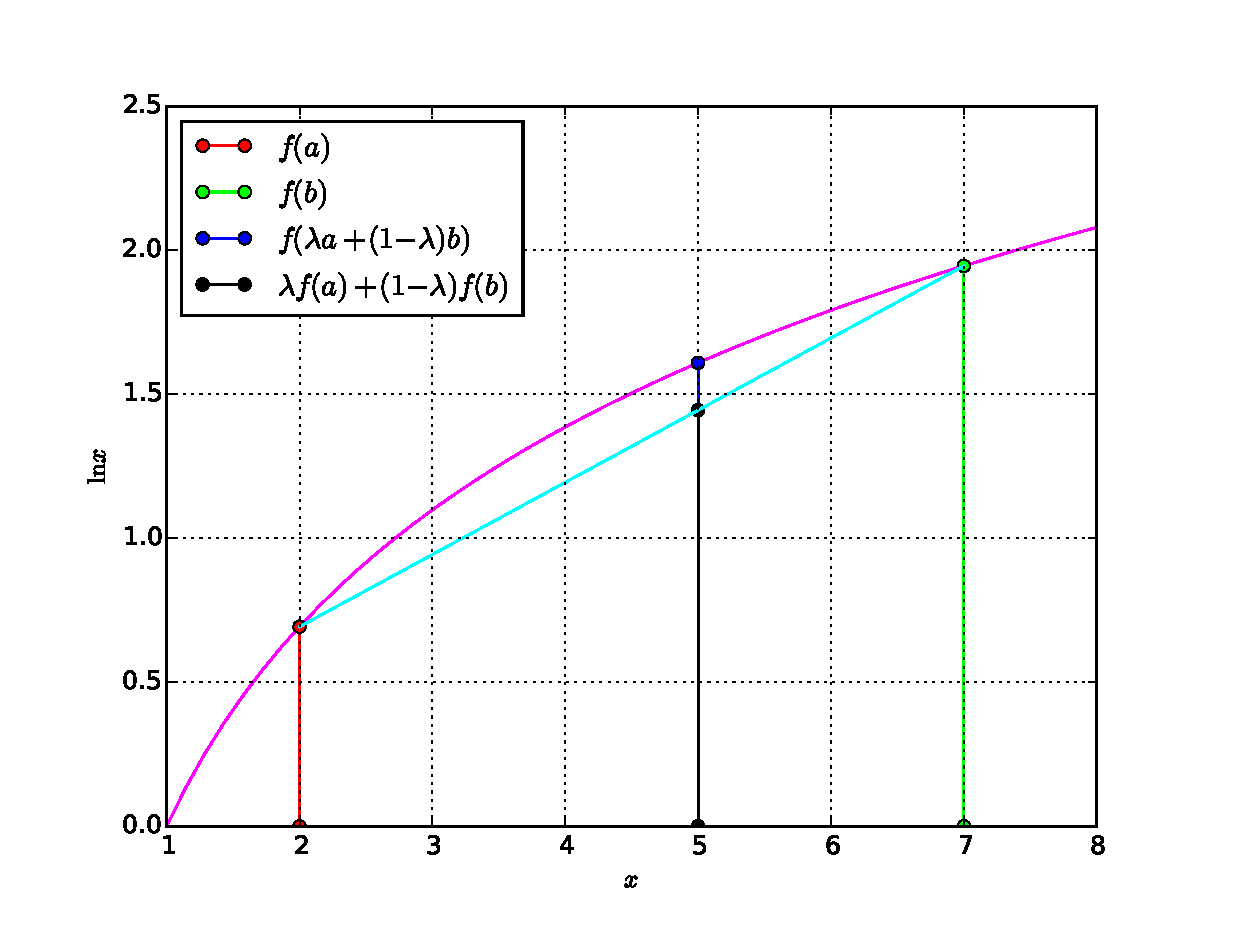
\includegraphics[width=\columnwidth]{./optimization/figs/1.1.eps}
\caption{ $\ln x$ versus $x$}.
\label{fig.1.1}	
\end{figure}
%
\item
Modify the above python script as follows to plot the parabola $f(x) = x^2$. Is it convex or concave?

\begin{lstlisting}
codes/optimization/1.2.py
\end{lstlisting}
%
\begin{figure}[!ht]
\centering
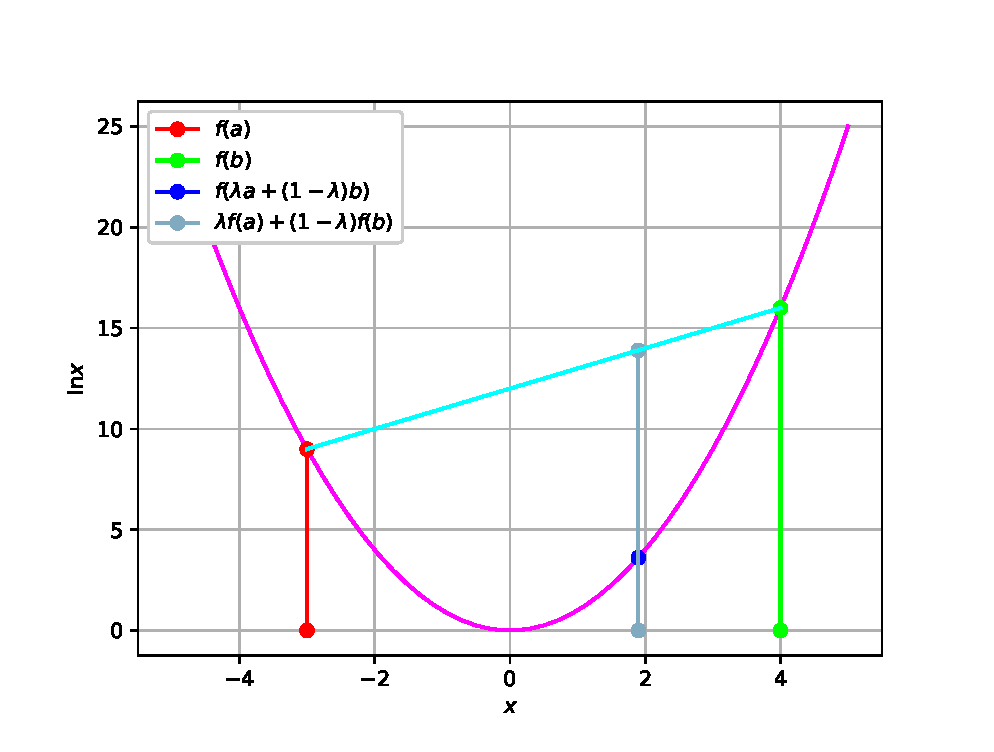
\includegraphics[width=\columnwidth]{./optimization/figs/1.2.eps}
\caption{ $x^2$ versus $x$}.
\label{fig.1.2}	
\end{figure}
%
\item
Execute the following script to obtain Fig. \ref{fig.1.3}. Comment.

%
\begin{lstlisting}
codes/optimization/1.3.py
\end{lstlisting}

%
\begin{figure}[!ht]
\centering
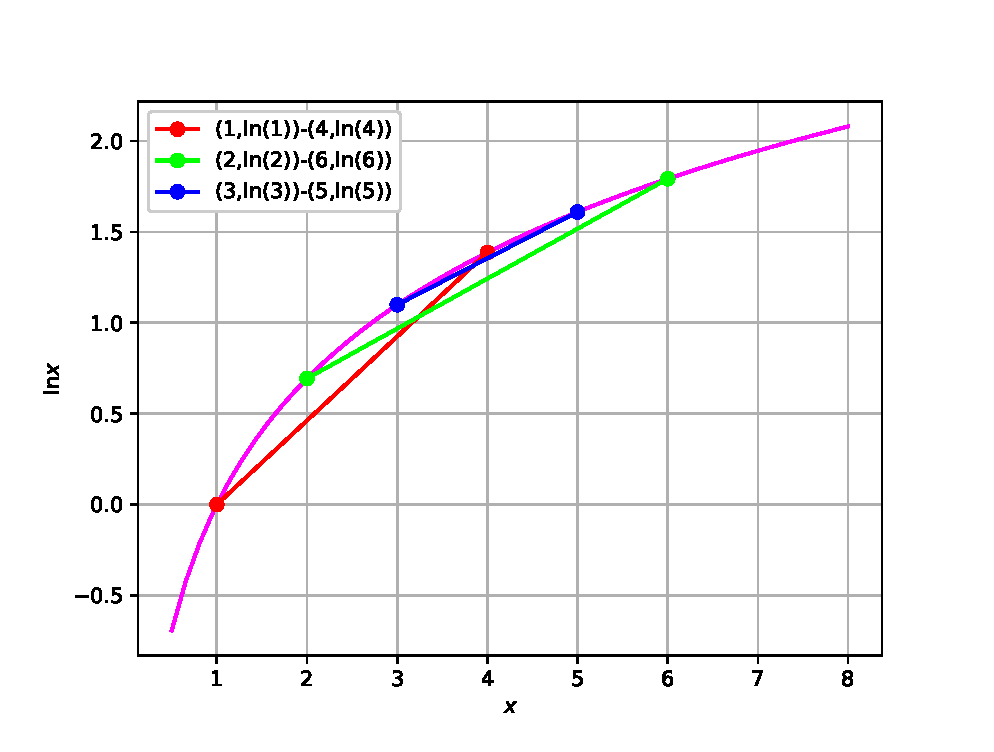
\includegraphics[width=\columnwidth]{./optimization/figs/1.3.eps}
\caption{ Segments are below the curve}.
\label{fig.1.3}	
\end{figure}
%
\item
Modify the script in the previous problem for $f(x) = x^2$.  What can you conclude?

\item
Let 
\begin{equation}
f(\mathbf{x}) = x_1x_2, \quad \mathbf{x} \in \mathbf{R}^2
\end{equation}
Sketch $f(\mathbf{x})$ and deduce whether it is convex.
\item Show that 
\begin{equation}
f(\mathbf{x}) = \vec{x}^T\vec{V}\vec{x} 
\end{equation}
%
and find $\vec{V}$.
\item Show that 
\begin{equation}
\frac{1}{2}\nabla^2f(\mathbf{x}) = \vec{V}
\end{equation}

\item Use \eqref{ch1_convex_def} to examine the convexity of $f(\vec{x})$.
\item How can you deduce the convexity of $f(\vec{x})$ using the eigenvalues of $\vec{V}$?
\item Show that $\vec{D}$ lies inside $\triangle ABC$ iff
\begin{align}
\vec{D} = \lambda_1\vec{A} + \lambda_2\vec{B} + \lambda_3\vec{C}
\end{align}
such that
\begin{align}
0 \le \lambda_1, \lambda_2, \lambda_3 &\le 1,
\\
0 \le \lambda_1+\lambda_2+\lambda_3 &\le 1,
\end{align}
\item Prove that the point $\myvec{4\\4}$ lies outside the triangle whose sides are the lines
\begin{align}
\myvec{3&4} \vec{x}&= 24
\\
\myvec{ 5 & - 3} \vec{x}&= 15
\\
\myvec{0 &1} \vec{x}&= 0
\end{align}


\end{enumerate}
%

\subsection{More on Convexity}
\renewcommand{\theequation}{\theenumi}
%\subsection{Problem}

\begin{enumerate}[label=\arabic*.,ref=\thesubsection.\theenumi]
\numberwithin{equation}{enumi}
%
%
\item Consider the optimization problem
\begin{align}
\label{eq:opt_def}
\max_{z} \frac{1}{\abs{z-1}}
\\
s.t. \quad \abs{z-2 + \j} \ge \sqrt{5}
\end{align}
%
Show that it can be reframed as
\begin{align}
\label{eq:opt_rev}
\min_{\vec{x}} \,\norm{\vec{x} - \vec{c}_1}^2
\\
 s.t. \quad  \norm{\vec{x} - \vec{c}_2}^2 \ge 5
%\min_{z} \abs{z-1}
%\\
% s.t. \quad \abs{z-2 + \j} \ge \sqrt{5}
\end{align}
%
where
\begin{align}
z &= \vec{x} = \myvec{x_1 \\ x_2},
%\\
\vec{c}_1 = \myvec{1 \\ 0},
%\\
\vec{c}_2 = \myvec{2 \\ -1}
\end{align}

%
%
%Then, 
%\begin{align}
%\Gamma: \abs{z-1} = \norm{\vec{x} - \vec{c}_1}^2,
%\end{align}
%where 
%\begin{align}
%\end{align}
%Similarly, 
%\begin{align}
%\Omega:\abs{z-2+\j} = \norm{\vec{x} - \vec{c}_2}^2,
%\end{align}
%where 
%\begin{align}
%\end{align}
%
%Let 
%\begin{align}
% \abs{z_0-1} = r
%\end{align}
%
%
\item Explain the optimization problem with a figure.
\\
\solution
Fig. \ref{fig:2019_1} explains \eqref{eq:opt_rev}
where $z_0$ is the set of points comprising of the intersection of the 
smallest circle $\Gamma:$ with the largest circle $\Omega: r_2 \ge 
\sqrt{5}$ 
with radii 
$r_1$ and 
$r_2 \ge \sqrt{5}$ respectively.
\begin{figure}[!ht]
\centering
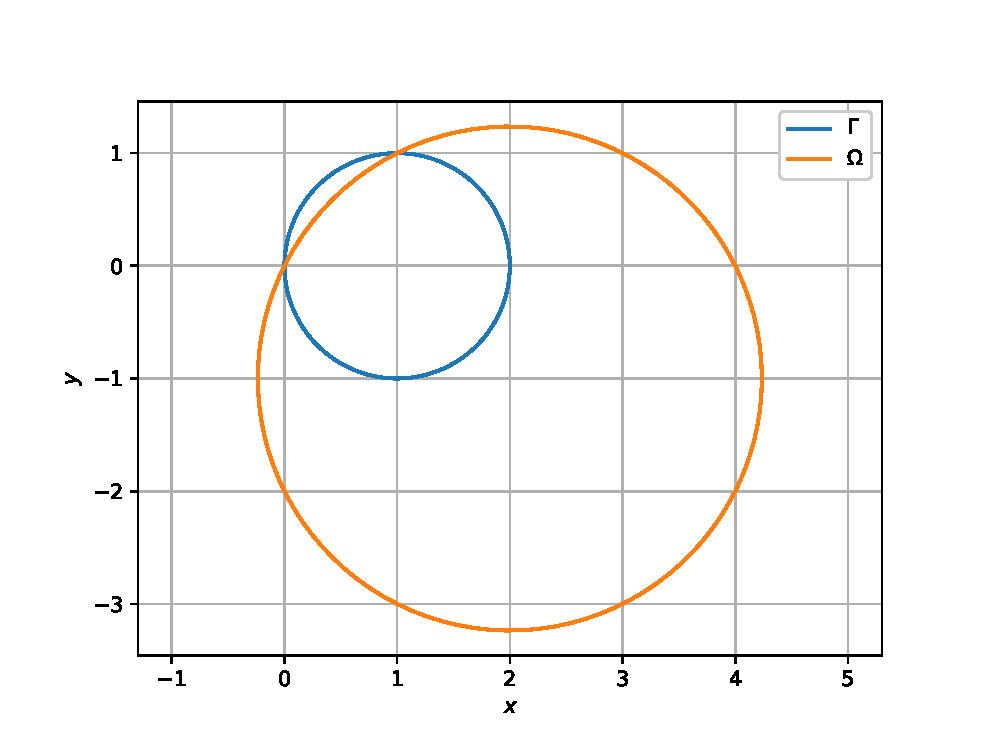
\includegraphics[width=\columnwidth]{./optimization/figs/2019_1_1.eps}
\caption{}
\label{fig:2019_1}
\end{figure}
%
\item Obtain the Lagrangian.
\\
\solution
The Lagrangian is 
\begin{align}
L \brak{\vec{x},\lambda} = \norm{\vec{x} - \vec{c}_1}^2 - \lambda 
\cbrak{\norm{\vec{x} - \vec{c}_2}^2-r_2^2}
\end{align}
\item Use the KKT conditions to obtain the minima.
\\
\solution
From the KKT conditions, 
\begin{align}
\frac{\partial L \brak{\vec{x},\lambda}}{\partial \vec{x}} &= 0
\\
\implies {\vec{x} - \vec{c}_1} - \lambda \brak{\vec{x} - \vec{c}_2} &= 0
\\
\implies \vec{x}  = \frac{\vec{c}_1 -\lambda  \vec{c}_2}{1-\lambda } &
\label{eq:opt_xlam}
\end{align}
%
and 
\begin{align}
\frac{\partial L \brak{\vec{x},\lambda}}{\partial \lambda} &= 0
\\
\implies \norm{\vec{x} - \vec{c}_2}^2-r_2^2 &= 0
\label{eq:opt_xnorm}
\end{align}
Substituting from \eqref{eq:opt_xlam} in \eqref{eq:opt_xnorm},
\begin{align}
\norm{\frac{\vec{c}_1 -\lambda  \vec{c}_2}{1-\lambda } - \vec{c}_2}^2-r_2^2 &= 0
\\
\implies \lambda = 1\pm \frac{\norm{\vec{c}_1 - \vec{c}_2}}{r_2}&
\\
= 1 \pm \sqrt{\frac{2}{5}}
%\label{eq:opt_xnorm}
\end{align}
Fig. \ref{fig:2019_1_2} plots $\Gamma$ for 
\begin{align}
\lambda = 1 - \sqrt{\frac{2}{5}}
\end{align}
\item If the maximum value is obtained at $z_0$, find the principal argument of
\begin{align}
\frac{4 - z_0-\bar{z}_0}{z_0-\bar{z}_0+2\j}
\end{align}
\\
\solution 
From \eqref{eq:opt_xlam},
\begin{align}
 \vec{x}_0  &= \frac{\vec{c}_1 -\lambda  \vec{c}_2}{1-\lambda } 
\\
\implies z_0 &= \frac{1}{1-\lambda}\brak{1-2\lambda + \j \lambda }
\\
\text{or, }\arg \frac{4 - z_0-\bar{z}_0}{z_0-\bar{z}_0+2\j} &= \frac{2 - \Re\cbrak{z_0}}{\j\brak{\Im\cbrak{z_0}+1}}
\\
&=\frac{2\brak{1-\lambda}-\brak{1-2\lambda}}{\j} 
\\
&= -\j
\end{align}
%
Thus, the principal argument is $-\frac{\pi}{2}$.
\begin{figure}[!ht]
\centering
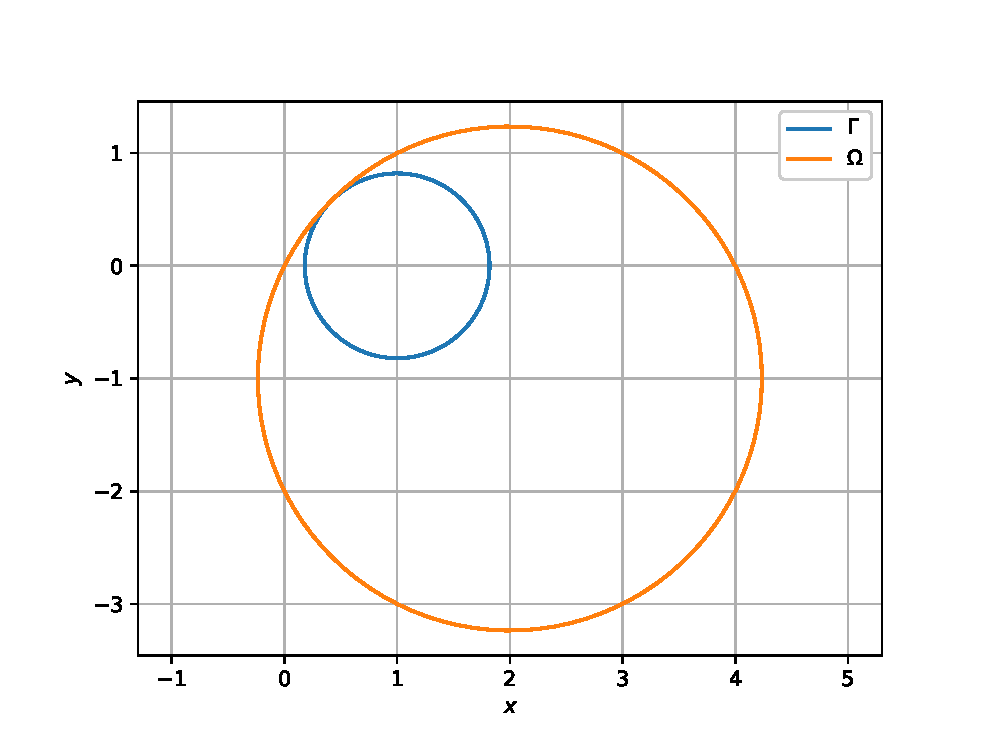
\includegraphics[width=\columnwidth]{./optimization/figs/2019_1_2.eps}
\caption{}
\label{fig:2019_1_2}
\end{figure}

%\begin{enumerate}[label=\theenumi.\arabic*
%,ref=\thesection.\theenumi]
\item Show that the set 
\begin{align}
D = \cbrak{\vec{x}:\norm{\vec{x}-\vec{C}_2} \ge r_2}, r_2 > 0
\end{align}
%
is nonconvex.
\\
\solution Let $\vec{x}_1 \in D$ and 
\begin{align}
\vec{x}_2 = 2\vec{C}_2-\vec{x}_1
\end{align}
Then 
\begin{align}
\norm{\vec{x}_2-\vec{C}_2} &= \norm{\vec{C}_2-\vec{x}_1} \ge r_2
\\
\implies \vec{x}_2 &\in D.
\end{align}
Suppose 
\begin{align}
\vec{x} = \theta\vec{x}_1+\brak{1-\theta}\vec{x}_2
\end{align}
For $\theta = \frac{1}{2}$,
\begin{align}
\vec{x} &= \vec{C}_2
\\
\implies \norm{\vec{x}-\vec{C}_2} &= 0,
\\
\text{or, } \vec{x} &\notin D
\end{align}
Thus, by definition, $D$ is not a convex set.
\end{enumerate}



\subsection{Gradient Descent Method}
\renewcommand{\theequation}{\theenumi}
\begin{enumerate}[label=\arabic*.,ref=\thesubsection.\theenumi]
\numberwithin{equation}{enumi}
\item Consider the problem of finding the square root of a number $c$.  This can be expressed as the equation
%
\begin{equation}
\label{eq:root}
x^2 -c= 0
\end{equation}
%

\item
Sketch the function for different values of $c$
%
\begin{equation}
f(x)= x^{3}-3xc
\end{equation}
%
and comment upon its convexity.

\item
Show that \eqref{eq:root} results from
\begin{align}
\min_{x}f(x)= x^{3}-3xc
\end{align}

\item
Find a numerical solution for \eqref{eq:root}.

\solution
A numerical solution for \eqref{eq:root} is obtained as
%
\begin{align}
x_{n+1}&=x_{n}-\mu f^{\prime}\brak{x}
\\
&=x_{n} -\mu \brak{3x_n^{2}-3c}
\label{eq:gradient}
\end{align}

%\begin{align}
%x_{n+1}&=x_{n}-{\frac {f(x_{n})}{f^{\prime}(x_{n})}}
%\\
%&=x_{n} -\frac{x^2_{n}-c}{2x_n} 
%\\
%&=\frac{1}{2}\sbrak{x_{n} +\frac{c}{x_n} }
%\label{eq:newton}
%\end{align}
%
where $x_0$ is an inital guess.
%
\item
Write a program to implement \eqref{eq:gradient}.

%
\solution Download and execute
\begin{lstlisting}
codes/optimization/square_root.py
\end{lstlisting}
\end{enumerate}


\subsection{Semi-definite Programming}
\renewcommand{\theequation}{\theenumi}
\begin{enumerate}[label=\arabic*.,ref=\thesubsection.\theenumi]
\numberwithin{equation}{enumi}

\item
%
\label{ch3_convex_ch2}
The problem
\begin{equation}
\min_{\mbf{X}} x_{11} + x_{12}
\end{equation}
%	
with constraints
\begin{align}
x_{11} + x_{22} &= 1 \\	
\mbf{X}
& \succeq 0 \quad  \brak{\text{$\succeq$ means positive definite}}
\end{align}
%
where
\begin{equation}
\mbf{X}=
\begin{pmatrix}
x_{11} & x_{12} \\
x_{12} & x_{22}
\end{pmatrix} 
\end{equation}
%
is known as a semi-definite program.  Find a numerical solution to this problem. Compare with the solution 
in problem  \ref{convex_sdp_eqiv}.
\label{prob:cvxopt}

\solution The {\em cvxopt} solver needs to be used in order to find a numerical solution.  For this, the given problem has to be reformulated as
\begin{align}
&\min_{\mbf{x}}  
\begin{pmatrix}
1 & 1 & 0
\end{pmatrix}
\begin{pmatrix}
x_{11} 
\\
x_{12}
\\
x_{22}
\end{pmatrix}
\quad \text{s.t}
\\
&
\begin{pmatrix}
1 & 0 & 1
\end{pmatrix}
\begin{pmatrix}
x_{11} 
\\
x_{12}
\\
x_{22}
\end{pmatrix}
=1
\end{align}
\begin{multline}
x_{11}
\begin{pmatrix}
-1 & 0 
\\
0 & 0
\end{pmatrix}
+
x_{12}
\begin{pmatrix}
0 & -1
\\
-1 & 0
\end{pmatrix}
+x_{22}
\begin{pmatrix}
0 & 0 
\\
0 & -1
\end{pmatrix}
\\
\preceq 
\begin{pmatrix}
0 & 0 
\\
0 & 0
\end{pmatrix}.
\end{multline}
%
The following script provides the solution to this problem.
\begin{lstlisting}
codes/optimization/3.1.py
\end{lstlisting}
%
\item
Frame Problem \ref{prob:cvxopt} in terms of matrices.

\solution
It is easy to verify that
\begin{equation}
x_{11} + x_{12} = 
\begin{pmatrix}
1 & 1
\end{pmatrix}
\mbf{X}^{T}
\begin{pmatrix}
1 
\\
0
\end{pmatrix}
\end{equation}
and
\begin{equation}
x_{11} + x_{22} = 
\begin{pmatrix}
1 & 0 & 0 & 1
\end{pmatrix}
\begin{pmatrix}
\mbf{X} & \mbf{0} \\
\mbf{0} & \mbf{X}
\end{pmatrix}
\begin{pmatrix}
1
\\
0 
\\
0
\\
1
\end{pmatrix}
\end{equation}
%
Thus, Problem \ref{prob:cvxopt} can be expressed as
\begin{equation}
\begin{split}
\min_{\mbf{X}} 
\begin{pmatrix}
1 & 1
\end{pmatrix}
\mbf{X}^{T}
\begin{pmatrix}
1 
\\
0
\end{pmatrix}
& \quad s.t
\\
\begin{pmatrix}
1 & 0 & 0 & 1
\end{pmatrix}
\begin{pmatrix}
\mbf{X} & \mbf{0} \\
\mbf{0} & \mbf{X}
\end{pmatrix}
\begin{pmatrix}
1
\\
0 
\\
0
\\
1
\end{pmatrix}
&=1,
\\
\mbf{X}
 & \succeq 0 
\end{split}
\label{prob:cvxpy}
\end{equation}
%	
\item
Solve \eqref{prob:cvxpy} using {\em cvxpy}.

%
\solution
\begin{lstlisting}
wget https://raw.githubusercontent.com/gadepall/school/master/linalg/book/optimizationcodes/3.1-cvx.py
\end{lstlisting}

\item
Minimize 
\begin{equation}
-x_{11} - 2x_{12} - 5x_{22}
\end{equation}
subject to
\begin{align}
\label{ch3_lin_mat_ineq_const}
2x_{11} + 3x_{12} + x_{22} &= 7 \\
x_{11} + x_{12} &\geq 1 \\
x_{11}, x_{12}, x_{22} &\geq 0 \\
\begin{pmatrix}
x_{11} & x_{12} \\
x_{12} & x_{22}
\end{pmatrix} & \succeq 0 
\end{align}
using {\em cvxpy}.

%\solution
%In this problem, there is an SDP inequality and several linear inequalities.  The linear inequalities can be combined to obtain the matrix inequality
%%
%\begin{equation}
%\label{ch3_lin_mat_ineq}
%\begin{pmatrix}
%x_{11} + x_{12}- 1 & 0  & 0 & 0\\
%0 & x_{11} & 0 & 0
%\\
%0 & 0 & x_{12} &  0
%\\
 %0 & 0 & 0 & x_{22} 
%\end{pmatrix}
 %\succeq 0 
%\end{equation}
%%
%\eqref{ch3_lin_mat_ineq} can be combined with the matrix inequality in \eqref{ch3_lin_mat_ineq_const} to obtain the composite SDP
%\begin{equation}
%\label{ch3_lin_mat_sdp_ineq}
%\begin{pmatrix}
%\begin{matrix}
%x_{11} + x_{12}- 1 & 0  & 0 & 0\\
%0 & x_{11} & 0 & 0
%\\
%0 & 0 & x_{12} &  0
%\\
 %0 & 0 & 0 & x_{22} 
%\end{matrix}
%& \mbf{0}
%\\
%\mbf{0} & \begin{matrix}
%x_{11} & x_{12} \\
%x_{12} & x_{22}
%\end{matrix}
%\end{pmatrix} 
 %\succeq 0 
%\end{equation}
%%
%For using  {\em cvxpy}, the SDP in \eqref{ch3_lin_mat_sdp_ineq} can be expressed as
%%
%\begin{equation}
 %x_{11}F_{0} + x_{12}F_1+x_{22}F_{2}\succeq B ,
%\end{equation}
%%
%where
%%
%\begin{align}
%F_{0} = 
%\begin{pmatrix}
%\begin{matrix}
%1 &
%\\
%& 1
%\end{matrix}
%& & \bigzero
%\\
%& 
%\begin{matrix}
%0 &
%\\
%& 0
%\end{matrix}
%&
%\\
%\bigzero& & 
 %\begin{matrix}
%1 &  \\
 %& 0
%\end{matrix}
%\end{pmatrix} 
%\\
%F_{1} = 
%\begin{pmatrix}
%\begin{matrix}
%1 &
%\\
%& 0
%\end{matrix}
%& & \bigzero
%\\
%& 
%\begin{matrix}
%1 &
%\\
%& 0
%\end{matrix}
%&
%\\
%\bigzero& & 
 %\begin{matrix}
%0 & 1 \\
%1 & 0
%\end{matrix}
%\end{pmatrix} 
%\\
%F_2 = 
%\begin{pmatrix}
%\begin{matrix}
%0 &
%\\
%& 0
%\end{matrix}
%& & \bigzero
%\\
%& 
%\begin{matrix}
%0 &
%\\
%& 1
%\end{matrix}
%&
%\\
%\bigzero& & 
 %\begin{matrix}
%0 &  \\
 %& 1
%\end{matrix}
%\end{pmatrix} 
%\end{align}
%and
%\begin{align}
%B=
%\begin{pmatrix}
%\begin{matrix}
%1 &
%\\
%& 0
%\end{matrix}
%& & \bigzero
%\\
%& 
%\begin{matrix}
%0 &
%\\
%& 0
%\end{matrix}
%&
%\\
%\bigzero& & 
 %\begin{matrix}
%0 &  \\
 %&0
%\end{matrix}
%\end{pmatrix} 
%\end{align}
%%
\item
	Repeat the above exercise by converting the problem into a convex optimization problem in two variables and using graphical plots.  

\item
	Solve the above problem using the KKT conditions.  Comment.

\end{enumerate}
	

\subsection{Linear Programming}
\renewcommand{\theequation}{\theenumi}
\begin{enumerate}[label=\arabic*.,ref=\thesubsection.\theenumi]
\numberwithin{equation}{enumi}
	
\item
\label{ch1_lp1}
	Graphically obtain a solution to the following 
	\begin{align}
\max_{\mbf{x}}	6x_1 + 5x_2
	\end{align}
	with constraints
	\begin{align}
	x_1 + x_2 &\leq 5\\
	3x_1 + 2x_2 &\leq 12\\
	\text{ where } x_1,x_2 &\geq 0
	\end{align}

%
\solution
The following program plots the solution in Fig. \ref{fig.4.1}
%	
\begin{lstlisting}
codes/optimization/4.1.py
\end{lstlisting}

%
\begin{figure}[!ht]
\centering
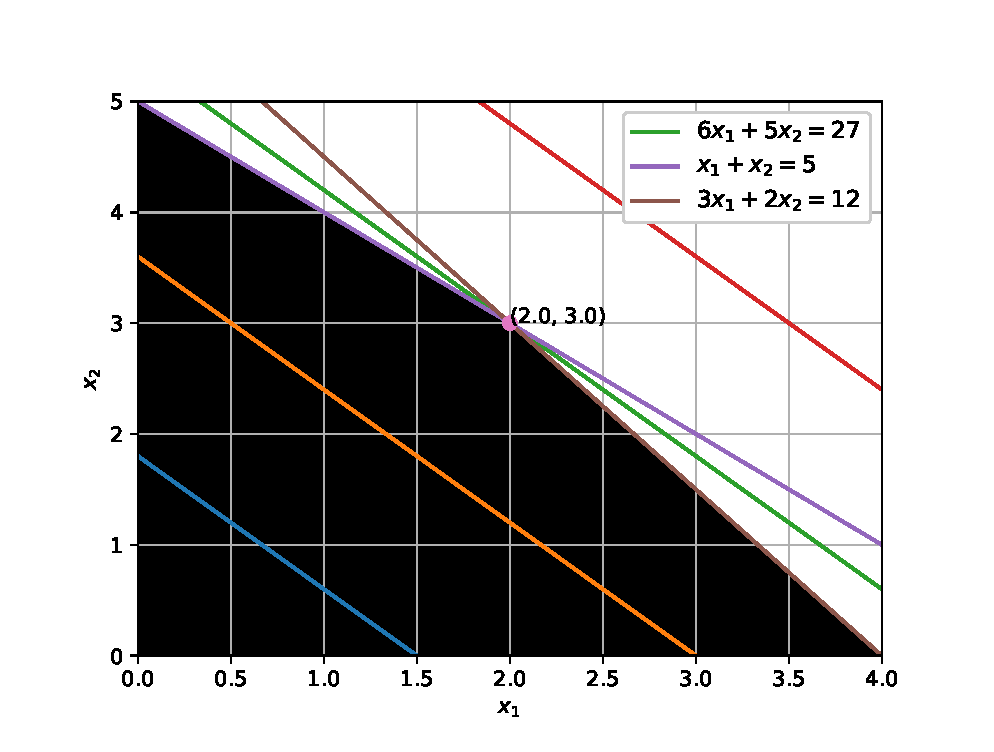
\includegraphics[width=\columnwidth]{./optimization/figs/4.1.eps}
\caption{ The cost function intersects with the two constraints at $\mbf{x} = \brak{2,3}$. }
\label{fig.4.1}	
\end{figure}
%
\item
	Now use {\em cvxpy} to obtain a solution to problem \ref{ch1_lp1}.

\solution
The given problem is expressed as follows
%
\begin{align}
\min_{\mbf{x}}	\mbf{c}^{T}\mbf{x}\quad s.t.
\\
\mbf{A}\mbf{x} \preceq \mbf{b}
\end{align}
%
where
%
\begin{equation}
\mbf{c}
=
\begin{pmatrix}
-6
\\
-5
\end{pmatrix},
\mbf{A} = 
\begin{pmatrix}
1 & 1
\\
3 & 2
\\
-1 & 0
\\
0 & -1
\end{pmatrix},
\mbf{b}
= 
\begin{pmatrix}
5
\\
12
\\
0
\\
0 
\end{pmatrix}
\end{equation}
%	
The desired solution is then obtained using the following program.
%\begin{lstlisting}
%codes/optimization/4.2.py
%\end{lstlisting}
%
%
%\item
%Repeat the previous exercise using {\em cvxpy}
%
%\solution
\begin{lstlisting}
codes/optimization/4.2-cvx.py
\end{lstlisting}

\item
	Verify your solution to the above problem using the method of Lagrange multipliers.

%
\item
	 Maximise $5x_1 + 3x_2$ w.r.t the constraints
	 \begin{align}
	 x_1 + x_2 &\leq 2 \nonumber\\
	 5x_1 + 2x_2 &\leq 10 \nonumber\\
	 3x_1 + 8x_2 &\leq 12 \nonumber\\
	 \text{ where } x_1,x_2 &\geq 0 \nonumber
	 \end{align}	

\end{enumerate}
%

\subsection{Exercises}
\renewcommand{\theequation}{\theenumi}
\begin{enumerate}[label=\arabic*.,ref=\thesubsection.\theenumi]
\numberwithin{equation}{enumi}

\item Let $\vec{P}$ be the point on the parabola
\begin{equation}
\label{eq:parab_circ_parab}
\vec{x}^T\myvec{0 & 0 \\ 0 & 1}\vec{x} -\myvec{8 & 0 }\vec{x} 
 = 0
\end{equation}
which is at a minimum distance from the centre $\vec{C}$ of the circle
\begin{equation}
\label{eq:parab_circ_circ}
\vec{x}^T\vec{x} +\myvec{0 & 12 }\vec{x} 
 = 1 
\end{equation} 
Find the equation of the circle passing through $\vec{C}$ and having its centre at $\vec{P}$. 
\item Let $\vec{P}$ 
be a point on the parabola
\begin{equation}
\vec{x}^T\myvec{1 & 0 \\ 0 & 0}\vec{x} +\myvec{0 & 4 }\vec{x} 
 = 0
\end{equation}
%%
Given that the distance of $\vec{P}$ from the centre of the circle
\begin{equation}
\vec{x}^T\vec{x} +\myvec{6 \\ 0 }\vec{x} + 8 = 0
\end{equation}
%
is minimum.  Find the equation of the tangent to the parabola at $\vec{P}$.
\item Find the eccentricity of the hyperbola whose length of the latus rectum is equal to 8 and the length of 
its conjugate axis is equal to half the distance between its foci. 
\item $\vec{P}$ and $\vec{Q}$ are two distinct points on the parabola
\begin{equation}
\vec{x}^T\myvec{0 & 0 \\ 0 & 1}\vec{x} -\myvec{4 & 0 }\vec{x} 
 = 0
\end{equation}
with parameters $t$ and $t_1$ respectively.  If the normal at $\vec{P} $ passes through $\vec{Q}$, then find 
the minimum value of $t_1^2$ using a descent algorithm.
\item A tangent at a point on the ellipse 
\begin{equation}
\vec{x}^TV\vec{x} =51
\end{equation}
%
where
\begin{equation}
V = \myvec{3 & 0 \\ 0 & 27}
\end{equation}
%
meets the coordinate axes at  $\vec{A}$  and  $\vec{B}$.  If   $\vec{O}$  be the origin, find the minimum area 
of $\triangle OAB$.
\item Find the shortest distance between the line 
\begin{equation}
\myvec{1 & -1 }\vec{x}  =0
\end{equation}
%
and the curve
\begin{equation}
\vec{x}^T\myvec{0 & 0 \\ 0 & 1}\vec{x} - \myvec{1 & 0}\vec{x} + 2 =0
\end{equation}
\item Let $S$ be the set of all complex numbers $z$ satisfying $\abs{z-2+\j} \ge \sqrt{5}$. If the complex number $z_0$ is such that $\frac{1}{\abs{z_0-1}}$ is the maximum of the set $\cbrak{\frac{1}{\abs{z-1}}: z \in S}$, find the principal argument of 
\begin{align}
\frac{4-z_0-\bar{z}_0}{z_0-\bar{z}_0+2\j}
\end{align}
\item Let $\omega \ne 1$ be a cube root of unity. Find the minimum of the set
\begin{align}
\abs{a+b\omega+c\omega^2}, 
\end{align}
%
where $a,b,c$ are distinct nonzero integers.
\item Let 
\begin{align}
\label{eq:mat_def}
\vec{M} = \myvec{\sin^4\theta & -1-\sin^2\theta \\ 1+ \cos^2\theta & \cos^4\theta} = \alpha\vec{I} + \beta \vec{M}^{-1}
\end{align}
where $\alpha, \beta$ are real functions of $\theta$ and $\vec{I}$ is the identity matrix. If 
\begin{align}
\alpha^{*} &= \min_{\theta}\alpha\brak{\theta}
\\
\beta^{*} &= \min_{\theta}\beta\brak{\theta}, 
\end{align}
find $\alpha^{*} + \beta^{*}$.
\item Find the minimum value of 
\begin{align}
\cos \brak{P+Q}
\cos \brak{Q+R}
\cos \brak{R+P}
\end{align}
%
in $\triangle PQR$.
\item Find the minimum value of $\alpha$ for which 
\begin{align}
4\alpha x^2 + \frac{1}{x} \ge 1, x > 0.
\end{align}
\item Let 
\begin{align}
S = S_1\cap S_2\cap S_3,
\end{align}
%
where
\begin{align}
S_1 &= \cbrak{z\in C: \abs{z}< 4}
\\
S_2 &= \cbrak{z\in C: \Im\sbrak{\frac{z-1+\j\sqrt{3}}{1-\j\sqrt{3}}}},
\\
S_3 &= \cbrak{z\in C: \Re\brak{z} > 0}
\end{align}
Find
\begin{align}
\min_{z\in S}\abs{1-3\j-z}
\end{align}
\item A line 
\begin{align}
L: \myvec{m -1}\vec{x} = -3
\end{align}
passes through
\begin{align}
\vec{E} = \myvec{0\\3}
\end{align}
and 
\begin{align}
\vec{x}\myvec{0 & 0 \\ 0 & 1}\vec{x} - \myvec{16 & 0}\vec{x} = 0, 0 \le \myvec{0 & 1}\vec{x} \le 6
\end{align}
%
at the point $\vec{F}$.  Find $m$ such that the area of $\triangle EFG$ is maximum.
\item If $\abs{z-3-2j} \le 2$, find
\begin{align}
\min_{z}\abs{2z-6+5\j}
\end{align}
\item Find 
\begin{align}
\max_{z}\abs{Arg\brak{\frac{1}{1-z}}}
\\
s.t\quad \abs{z} = 1, z \ne 1.
\end{align}
\item Find the maximum value of the function 
\begin{align}
f(x) = 2x^3-15x^2+36x-48
\end{align}
on the set 
\begin{align}
A = \cbrak{x : x^2+20 \le 9x}
\end{align}
\item Find the minimum distance of a point on the curve 
\begin{align}
\vec{x}^T\myvec{1 & 0 \\ 0 & 1}\vec{x} + \myvec{0 -1}\vec{x}=4
\end{align}
%
from the origin.
\item Find 
\begin{align}
\min_{z}\abs{z+\frac{1}{2}}
\\
s.t\quad \abs{z} \ge 2
\end{align}
\item Find  the minimum value of
\begin{align}
\tan A + \tan B
\\
s.t \quad A+B=6,
\\
A, B \ge 0
\end{align}
\item Show that 
\begin{multline}
\sin A_1+\sin A_2 + \dots + \sin A_n 
\\
\le n \sin \brak{\frac{A_1+A_2+\dots + A_n}{n}}
\\
0 < A_i < \pi, i = 1, 2, \dots , n, n \ge 1
\end{multline}
\item Let $\vec{F}_1, \vec{F}_2$ be the foci of the standard ellipse with parameters $a$ and $b$.  If $\vec{P}$ be any point on the ellipse, find the maximum area of $\triangle PF_1F_2$.
\item A circle $\norm{\vec{x}}=1$ intersects the $X-$ axis at $\vec{P}$ and $\vec{Q}$.  Another circle with centre $\vec{Q}$ intersects this circle above the $X-$ axis at $\vec{R}$ and the line segent $PQ$ at $\vec{S}$.  Find the maximum area of $\triangle QSR$.
\item Let $\vec{M}$ be a fixed point in the first quadrant.   A line through $\vec{M}$ intersects the positive axes at $\vec{P}, \vec{Q}$ respectively. If $\vec{O}$ be the origin, find the minimum area of $\triangle OPQ$.
\end{enumerate}

\section{Matrices}
\subsection{Properties}
\renewcommand{\theequation}{\theenumi}
\begin{enumerate}[label=\arabic*.,ref=\thesubsection.\theenumi]
\numberwithin{equation}{enumi}
\item Show that 
\begin{align}
\min_{a,b,c} \abs{a + b\omega + c\omega^2}^2
\end{align}
%
where $\omega^3 = 1, \omega \ne 1$ and $a,b,c$ are distinct nonzero integers
can be expressed as
\begin{align}
\label{eq:13_opt}
\min_{\vec{x}} \frac{1}{2}\vec{x}^T\vec{A}\vec{x}
\end{align}
%
where 
\begin{align}
\vec{x}&= \myvec{a \\ b \\c}, 
\vec{A}= 2\vec{P}^T\vec{P},
\\
\vec{P}&= \myvec{1 & \cos \theta & -\cos \theta \\ 0 & \sin \theta & \sin \theta},
\theta = \frac{\pi}{3} 
\end{align}
\item Show that 
\begin{align}
\label{eq:13_A}
\vec{A}  = \myvec{
2 & 1 & -1 \\ 
1 & 2 & 1
\\
-1 & 1 & 2
}
\end{align}
%
\solution 
\begin{align}
\vec{A}&= \myvec{1 &  0 \\ \cos \theta & \sin \theta  \\ -\cos \theta  & \sin \theta} 
\myvec{1 & \cos \theta & -\cos \theta \\ 0 & \sin \theta & \sin \theta} 
\nonumber \\
&=\myvec{
1 & \cos \theta & -\cos \theta \\ 
\cos \theta & 1 & -\cos 2\theta
\\
-\cos \theta & -\cos 2\theta & 1
},
\end{align}
resulting in \eqref{eq:13_A}.
\begin{align}
\because \cos 2 \theta = -\cos \theta = -\frac{1}{2}
\end{align}
\item Show that the characteristic equation of $\vec{A}$ is 
\begin{align}
f(\lambda) = \lambda^3 -6\lambda^2 + 9\lambda
\end{align}
\item Show that the eigenvalues of $\vec{A}$ are 0 and 3.
\item Verify that $tr\brak{\vec{A}}$ is the sum of its eigenvalues.
\item Verify that $\det\brak{\vec{A}}$ is the product of  its eigenvalues.
\item Show that $\vec{A}$ is positive definite.
\item Show that $\vec{x}^{T}\vec{A}\vec{x}$ is convex.
\item Show that the unconstrained $\vec{x}$ that minimizes $\vec{x}^{T}\vec{A}\vec{x}$ is given by the line
\begin{align}
\vec{x} = k \myvec{1 \\ -1 \\ 1}
\end{align}
\item Find $\vec{y}$ such that 
\begin{align}
\vec{A}\vec{y} = \lambda\vec{y}
\end{align}
where $\lambda$ is an eigenvalue of $\vec{A}$.
\item Show that 
\begin{align}
\vec{A} = \vec{P}^{-1} \vec{D}\vec{P}
\end{align}
%
where $\vec{D}$  is a diagonal matrix comprising of the eigenvalues of $\vec{A}$
and the columns of $\vec{P}$ are the corresponding eigenvectors.
\item Find $\vec{U}$ such that 
\begin{align}
\vec{A} = \vec{U}^{T} \vec{D}\vec{U}, \vec{U}^{T} \vec{U} = \vec{I}
\end{align}
\item Show that 
\begin{align}
\vec{x}^T \vec{A}\vec{x}  = 3 \vec{v}^{T} \vec{v},
\end{align}
where
\begin{align}
\vec{v} = \vec{U}\vec{x}
\end{align}
%
\item Show that when the entries of $\vec{x}$ are unequal and integers, the solution of \eqref{eq:13_opt} can be expressed as
\begin{align}
\vec{x} = \myvec{1 \\ -1 \\ 0} + c\myvec{1 \\ -1 \\ 1}
\end{align}

%\nonumber \\
%\\
%\solution The desired $\vec{x}$ is obtained by 
%\begin{align}
%\frac{d}{d\vec{x}}\vec{x}^{T}\vec{A}\vec{x} &= \vec{0}
%\nonumber \\
%\implies \vec{A}\vec{x} &= \vec{0}
%\end{align}
\end{enumerate}

\subsection{Cayley-Hamilton Theorem}
\renewcommand{\theequation}{\theenumi}
\begin{enumerate}[label=\arabic*.,ref=\thesubsection.\theenumi]
\numberwithin{equation}{enumi}

\item Let
\begin{align}
\label{eq:cayley_mat_def}
\vec{M} = \myvec{\sin^4\theta & -1-\sin^2\theta \\ 1+ \cos^2\theta & \cos^4\theta} = \alpha\vec{I} + \beta \vec{M}^{-1}
\end{align}
where $\alpha, \beta$ are real functions of $\theta$ and $\vec{I}$ is the identity matrix. Find the characteristic equation of $\vec{M}$.
\\
\solution \eqref{eq:cayley_mat_def} can be expressed as
\begin{align}
\vec{M}^2 -\alpha\vec{M} - \beta \vec{I} = 0
\end{align}
%
which yields   the characteristic equation of $\vec{M}$ as
\begin{align}
\lambda^2 -\alpha\lambda - \beta  = 0
\end{align}
\item Find $\alpha$ and $\beta$.
\\
\solution
Since the sum of the eigenvalues is equal to the trace and the determinant is the product of eigenvalues,
\begin{align}
 \alpha &= \sin^4\theta + \cos^4\theta 
\\
  \beta & = -\sin^4\theta \cos^4\theta + \brak{1+\sin^2\theta}\brak{ 1+ \cos^2\theta}
\end{align}
\item If 
\begin{align}
\alpha^{*} &= \min_{\theta}\alpha\brak{\theta}
\\
\beta^{*} &= \min_{\theta}\beta\brak{\theta}, 
\end{align}
find $\alpha^{*} + \beta^{*}$.
\\
\solution 
\begin{align}
\because  \alpha &= \sin^4\theta + \cos^4\theta = 1 - \frac{\sin^2 2\theta}{2},
\\
\alpha^{*} &= \frac{1}{2}, 
\end{align}
Similarly,
\begin{align}
 - \beta & = \sin^4\theta \cos^4\theta + \brak{1+\sin^2\theta}\brak{ 1+ \cos^2\theta}
\\
&=2 + \frac{\sin^2 2\theta}{4} + \frac{\sin^4 2\theta}{16}
\\
&= \brak{\frac{\sin^2 2\theta}{4}+\frac{1}{2}}^2+ \frac{7}{4} 
\end{align}
Thus,
\begin{align}
 \beta^{*} &= -\frac{37}{16}
\\
\implies \alpha^{*}+\beta^{*} &= -\frac{29}{16}
\end{align}
\end{enumerate}

\subsection{Trace}
\renewcommand{\theequation}{\theenumi}
\begin{enumerate}[label=\arabic*.,ref=\thesubsection.\theenumi]
\numberwithin{equation}{enumi}
\item Obtain the  $3 \times 3$ matrices $\cbrak{\vec{P}_k}_{k=1}^{6}$ from permutations of the  vectors
\begin{align}
\vec{v}_1 = \myvec{0 \\ 0 \\ 1},
\vec{v}_2 = \myvec{0 \\ 1 \\ 0},
\vec{v}_3 = \myvec{1 \\ 0 \\ 0}
\end{align}
%
%
\item Let 
\begin{align}
\vec{X} = \sum_{k=1}^{6}\vec{P}_k\myvec{2 & 1 & 3 \\ 1 & 0 & 2 \\ 3 & 2 & 1}\vec{P}_k^T.
\end{align}
Given 
\begin{align}
\vec{X}\myvec{1 \\1 \\1} = \alpha\myvec{1 \\1 \\1},
\label{eq:2019_qp2_1_alpha}
\end{align}
is
$\alpha= 30$?
\\
\solution 
\begin{align}
\because \vec{P}_k^T\myvec{1 \\1 \\1} &=  \myvec{1 \\1 \\1},
\nonumber \\
\vec{X}\myvec{1 \\1 \\1} &= \sum_{k=1}^{6}\vec{P}_k\myvec{2 & 1 & 3 \\ 1 & 0 & 2 \\ 3 & 2 & 1}\vec{P}_k^T\myvec{1 \\1 \\1} 
\nonumber \\
&= \sum_{k=1}^{6}\vec{P}_k\myvec{2 & 1 & 3 \\ 1 & 0 & 2 \\ 3 & 2 & 1}\myvec{1 \\1 \\1} 
\nonumber \\
&= \sum_{k=1}^{6}\vec{P}_k\myvec{5 \\3 \\5} =2\myvec{1 & 1 & 1 \\ 1 & 1 & 1 \\ 1 & 1 & 1}\myvec{6 \\3 \\6}
\nonumber \\
&= 30\myvec{1 \\1 \\1} 
\end{align}
%
Thus, $\alpha=30$.
\item Is $\vec{X}$  symmetric?
\\
\solution Yes. Trivial.
\item Show that 
\begin{align}
\label{eq:2019_qp2_1_I}
\vec{P}_k\vec{P}_k^T = \vec{I}
\end{align}
\solution
\begin{align}
\vec{P}_k = \myvec{\vec{v}_{k1}^T\\\vec{v}_{k2}^T\\\vec{v}_{k3}^T}
\end{align}
%
where $\vec{v}_{ki}, i = 1,2,3$ are from the standard basis.  Then,
\begin{align}
\vec{P}_k\vec{P}_k^T &= \myvec{\vec{v}_{k1}^T\\\vec{v}_{k2}^T\\\vec{v}_{k3}^T}\myvec{\vec{v}_{k1}&\vec{v}_{k2}&\vec{v}_{k3}}
 \vec{I}
\nonumber
\\
\because 
\vec{v}_{ji}^T\vec{v}_{kj} &= \delta_{jk}
\end{align}
%
\item For $2\times 2$ matrices $\vec{A},\vec{B}$, verify that 
\begin{align}
tr\brak{AB}=tr\brak{BA}
\end{align}
%
Show that this is true for any square matrix.
\item Verify if the sum of the diagonal entries of $X$ is 18.
\\
\solution 
\begin{align}
\text{tr}\brak{\vec{X}} &= \sum_{k=1}^{6}\text{tr}\cbrak{\vec{P}_k\myvec{2 & 1 & 3 \\ 1 & 0 & 2 \\ 3 & 2 & 1}\vec{P}_k^T}
\nonumber \\
&= \sum_{k=1}^{6}\text{tr}\cbrak{\myvec{2 & 1 & 3 \\ 1 & 0 & 2 \\ 3 & 2 & 1}\vec{P}_k\vec{P}_k^T}
\nonumber \\
&= \sum_{k=1}^{6}\text{tr}\myvec{2 & 1 & 3 \\ 1 & 0 & 2 \\ 3 & 2 & 1} = 6\times 3 = 18
\end{align}
after substituting from \eqref{eq:2019_qp2_1_I}.
%
\item Is $\vec{X}-30\vec{I}$ invertible?
\\
\solution From \eqref{eq:2019_qp2_1_alpha},
\begin{align}
\vec{X}\myvec{1 \\1 \\1} &=30\vec{I}\myvec{1 \\1 \\1} 
\nonumber \\
\implies \brak{\vec{X}-30\vec{I}}\myvec{1 \\1 \\1}  &=0
\end{align}
If $\brak{\vec{X}-30\vec{I}}^{-1}$ exists,
\begin{align}
\brak{\vec{X}-30\vec{I}}^{-1}\brak{\vec{X}-30\vec{I}}\myvec{1 \\1 \\1}  &=0
\nonumber \\
\implies \myvec{1 \\1 \\1}  &=\vec{0}
\end{align}
%
which is a contradiction.  Hence, $\vec{X}-30\vec{I}$ is not invertible.
%
\item For any two $3 \times 3$ matrices $A$ and $B$, let $A+B = 2B^T$ and $3A+2B=I_3$.  Which of the following 
is true?
\begin{enumerate}
\item $5A+10B=2I_3$.
\item $10A+5B=3I_3$.
\item $2A+B=3I_3$.
\item $3A+6B=2I_3$.
\end{enumerate}
\end{enumerate}

\subsection{Eigenvector and Null Space}
\renewcommand{\theequation}{\theenumi}
\begin{enumerate}[label=\arabic*.,ref=\thesubsection.\theenumi]
\numberwithin{equation}{enumi}

\item Let 
\begin{align}
\vec{P} = \myvec{1 & 1 & 1 \\ 0 & 2 & 2 \\ 0 & 0 & 3}, 
\vec{Q} = \myvec{2 & x & x \\ 0 & 4 & 0 \\ x & x & 6}
\label{eq:2019_qp2_2_q}
\end{align}
%

\item Find $x$ such that $PQ=QP$.
%
\\
\solution 
\begin{align}
\because \vec{Q} &= \myvec{2 & 0 & 0 \\ 0 & 4 & 0 \\ 0 & 0 & 6} +x\myvec{0 & 1 & 1 \\ 0 & 0 & 0 \\ 1 & 1 & 0}, 
\end{align}
\begin{align}
\vec{P}\vec{Q} = 
 \myvec{2 & 4 & 6 \\ 0 & 8 & 12 \\ 0 & 0 & 18}+x\myvec{1 & 2 & 1 \\ 2 & 2 & 0 \\ 3 & 3 & 0}
\end{align}
and 
\begin{multline}
\vec{Q}\vec{P} = 
\myvec{2 & 2 & 2 \\ 0 & 8 & 8 \\ 0 & 0 & 18}+x\myvec{0 & 2 & 5 \\ 0 & 0 & 0 \\ 1 & 3 & 3} 
\end{multline}
%
Thus, 
\begin{align}
\vec{P}\vec{Q} = \vec{Q}\vec{P} 
\implies 
\myvec{0 & 2 & 4 \\ 0 & 0 & 4 \\ 0 & 0 & 0} &= x\myvec{-1 & 0 & 4 \\ -2 & -2 & 0 \\ -2 & 0 & 3}
\end{align}
which has no solution.
\item If 
\begin{align}
\vec{R} = \vec{P}\vec{Q}\vec{P}^{-1},
\end{align}
verify whether 
\begin{align}
\det{\vec{R}}= 
\det\myvec{2 & x & x \\ 0 & 4 & 0 \\ x & x & 5} + 8
\end{align}
for all $x$.
\\
\solution 
\begin{align}
\det(\vec{R}) &= \det(\vec{P})\det(\vec{Q})\det(\vec{P})^{-1}=\det(\vec{Q})
\nonumber \\
&= 4\brak{12-x^2}
\end{align}
%
Thus, 
\begin{multline}
\det(\vec{R}) - \det\myvec{2 & x & x \\ 0 & 4 & 0 \\ x & x & 5}
\\
= 4\cbrak{\brak{12-x^2}-\brak{10-x^2}}
\\
= 8
\end{multline}
%
which is true.
\item For $x= 0$, if 
\begin{align}
\label{eq:2019_qp2_2_ab}
\vec{R}\myvec{1 \\ a \\ b} = 6\myvec{1 \\ a \\ b}, 
\end{align}
%
then show that 
\begin{align}
a+b = 5.
\end{align}
\solution For $x=0$, 
\begin{align}
\vec{R} = \vec{P}\vec{Q}\vec{P}^{-1},
\end{align}
%
where $\vec{Q}$ is a diagonal matrix.  This is the eigenvalue decomposition of $\vec{R}$.  Thus, 
\begin{align}
\label{eq:2019_qp2_2_6eig}
\vec{R}\myvec{1 \\ 2 \\ 3} = 6\myvec{1 \\ 2 \\ 3}, 
\end{align}
%
where 
\begin{align}
\myvec{1 \\ 2 \\ 3}
\end{align}
%
is the eigenvector corresponding to the eigenvalue $6$. Comparing with \eqref{eq:2019_qp2_2_6eig},
\begin{align}
a=2,b=3 \implies a+b = 5.
\end{align}
%
\item For $x = 1$, verify if  there exists a  vector $\vec{y}$ for which $\vec{R}\vec{y} = \vec{0}$. 
\\
\solution 
\begin{align}
\vec{R}\vec{y} &= \vec{0} \implies \vec{P}\vec{Q}\vec{P}^{-1}\vec{y} = \vec{0}
\nonumber \\
\implies \vec{Q} \vec{z}&= \vec{0},
\label{eq:2019_qp2_2_null}
\end{align}
%
where 
\begin{align}
\label{eq:2019_qp2_2_yz}
\vec{z} = \vec{P}^{-1}\vec{y} 
\end{align}
For $x=1$, \eqref{eq:2019_qp2_2_q} and \eqref{eq:2019_qp2_2_null} yield
\begin{align}
\label{eq:2019_qp2_2_x1}
\myvec{2 & 1 & 1 \\ 0 & 4 & 0 \\ 1 & 1 & 6}\vec{z} &= \vec{0} 
\end{align}
Using row reduction,
\begin{align}
%\label{eq:2019_qp2_2_x1}
\myvec{2 & 1 & 1 \\ 0 & 4 & 0 \\ 1 & 1 & 6} &\leftrightarrow
\myvec{2 & 1 & 1 \\ 0 & 1 & 0 \\ 0 & 1 & 11} \leftrightarrow
\myvec{1 & 0 & -5 \\ 0 & 1 & 0 \\ 0 & 1 & 11} \leftrightarrow
\nonumber \\
\myvec{1 & 0 & -5 \\ 0 & 1 & 0 \\ 0 & 0 & 11} &
\end{align}
%
Thus, $\vec{Q}^{-1}$ exists and 
\begin{align}
\vec{z} = \vec{0} \implies \vec{y}= \vec{0}
\end{align}
upon substituting from \eqref{eq:2019_qp2_2_yz}.
This implies that the null space of $\vec{R}$ is empty. 
\end{enumerate}


\subsection{JEE Exercises}
\renewcommand{\theequation}{\theenumi}
\begin{enumerate}[label=\arabic*.,ref=\thesubsection.\theenumi]
\numberwithin{equation}{enumi}

%\documentclass[journal,12pt,twocolumn]{IEEEtran}
%\usepackage{setspace}
%\usepackage{gensymb}
%\usepackage{caption}
%\usepackage{subfiles}
%%\usepackage{multirow}
%%\usepackage{multicolumn}
%%\usepackage{subcaption}
%%\doublespacing
%\singlespacing
%\usepackage{csvsimple}
%\usepackage{amsmath}
%\usepackage{multicol}
%%\usepackage{enumerate}
%\usepackage{amssymb}
%%\usepackage{graphicx}
%\usepackage{newfloat}
%%\usepackage{syntax}
%\usepackage{listings}
%%\usepackage{iithtlc}
%\usepackage{color}
%\usepackage{tikz}
%\usetikzlibrary{shapes,arrows}
%
%
%
%%\usepackage{graphicx}
%%\usepackage{amssymb}
%%\usepackage{relsize}
%%\usepackage[cmex10]{amsmath}
%%\usepackage{mathtools}
%%\usepackage{amsthm}
%%\interdisplaylinepenalty=2500
%%\savesymbol{iint}
%%\usepackage{txfonts}
%%\restoresymbol{TXF}{iint}
%%\usepackage{wasysym}
%\usepackage{amsthm}
%\usepackage{mathrsfs}
%\usepackage{txfonts}
%\usepackage{stfloats}
%\usepackage{cite}
%\usepackage{cases}
%\usepackage{mathtools}
%\usepackage{caption}
%\usepackage{enumerate}
%\usepackage{tfrupee}	
%\usepackage{enumitem}
%\usepackage{amsmath}
%%\usepackage{xtab}
%\usepackage{longtable}
%\usepackage{multirow}
%%\usepackage{algorithm}
%%\usepackage{algpseudocode}
%\usepackage{enumitem}
%\usepackage{mathtools}
%\usepackage{hyperref}
%%\usepackage[framemethod=tikz]{mdframed}
%\usepackage{listings}
%    %\usepackage[latin1]{inputenc}                                 %%
%    \usepackage{color}                                            %%
%    \usepackage{array}                                            %%
%    \usepackage{longtable}                                        %%
%    \usepackage{calc}                                             %%
%    \usepackage{multirow}                                         %%
%    \usepackage{hhline}                                           %%
%    \usepackage{ifthen}                                           %%
%  %optionally (for landscape tables embedded in another document): %%
%    \usepackage{lscape}     
%
%
%\usepackage{url}
%\def\UrlBreaks{\do\/\do-}
%
%
%%\usepackage{stmaryrd}
%
%
%%\usepackage{wasysym}
%%\newcounter{MYtempeqncnt}
%\DeclareMathOperator*{\Res}{Res}
%%\renewcommand{\baselinestretch}{2}
%\renewcommand\thesection{\arabic{section}}
%\renewcommand\thesubsection{\thesection.\arabic{subsection}}
%\renewcommand\thesubsubsection{\thesubsection.\arabic{subsubsection}}
%
%\renewcommand\thesectiondis{\arabic{section}}
%\renewcommand\thesubsectiondis{\thesectiondis.\arabic{subsection}}
%\renewcommand\thesubsubsectiondis{\thesubsectiondis.\arabic{subsubsection}}
%
%% correct bad hyphenation here
%\hyphenation{op-tical net-works semi-conduc-tor}
%
%%\lstset{
%%language=C,
%%frame=single, 
%%breaklines=true
%%}
%
%%\lstset{
%	%%basicstyle=\small\ttfamily\bfseries,
%	%%numberstyle=\small\ttfamily,
%	%language=Octave,
%	%backgroundcolor=\color{white},
%	%%frame=single,
%	%%keywordstyle=\bfseries,
%	%%breaklines=true,
%	%%showstringspaces=false,
%	%%xleftmargin=-10mm,
%	%%aboveskip=-1mm,
%	%%belowskip=0mm
%%}
%
%%\surroundwithmdframed[width=\columnwidth]{lstlisting}
%\def\inputGnumericTable{}                                 %%
%\lstset{
%%language=C,
%frame=single, 
%breaklines=true,
%columns=fullflexible
%}
% 
%
%\begin{document}
%%
%\tikzstyle{block} = [rectangle, draw,
%    text width=3em, text centered, minimum height=3em]
%\tikzstyle{sum} = [draw, circle, node distance=3cm]
%\tikzstyle{input} = [coordinate]
%\tikzstyle{output} = [coordinate]
%\tikzstyle{pinstyle} = [pin edge={to-,thin,black}]
%
%\theoremstyle{definition}
%\newtheorem{theorem}{Theorem}[section]
%\newtheorem{problem}{Problem}
%\newtheorem{proposition}{Proposition}[section]
%\newtheorem{lemma}{Lemma}[section]
%\newtheorem{corollary}[theorem]{Corollary}
%\newtheorem{example}{Example}[section]
%\newtheorem{definition}{Definition}[section]
%%\newtheorem{algorithm}{Algorithm}[section]
%%\newtheorem{cor}{Corollary}
%\newcommand{\BEQA}{\begin{eqnarray}}
%\newcommand{\EEQA}{\end{eqnarray}}
%\newcommand{\define}{\stackrel{\triangle}{=}}
%
%\bibliographystyle{IEEEtran}
%%\bibliographystyle{ieeetr}
%
%\providecommand{\nCr}[2]{\,^{#1}C_{#2}} % nCr
%\providecommand{\nPr}[2]{\,^{#1}P_{#2}} % nPr
%\providecommand{\mbf}{\mathbf}
%\providecommand{\pr}[1]{\ensuremath{\Pr\left(#1\right)}}
%\providecommand{\qfunc}[1]{\ensuremath{Q\left(#1\right)}}
%\providecommand{\sbrak}[1]{\ensuremath{{}\left[#1\right]}}
%\providecommand{\lsbrak}[1]{\ensuremath{{}\left[#1\right.}}
%\providecommand{\rsbrak}[1]{\ensuremath{{}\left.#1\right]}}
%\providecommand{\brak}[1]{\ensuremath{\left(#1\right)}}
%\providecommand{\lbrak}[1]{\ensuremath{\left(#1\right.}}
%\providecommand{\rbrak}[1]{\ensuremath{\left.#1\right)}}
%\providecommand{\cbrak}[1]{\ensuremath{\left\{#1\right\}}}
%\providecommand{\lcbrak}[1]{\ensuremath{\left\{#1\right.}}
%\providecommand{\rcbrak}[1]{\ensuremath{\left.#1\right\}}}
%\theoremstyle{remark}
%\newtheorem{rem}{Remark}
%\newcommand{\sgn}{\mathop{\mathrm{sgn}}}
%\providecommand{\abs}[1]{\left\vert#1\right\vert}
%\providecommand{\res}[1]{\Res\displaylimits_{#1}} 
%\providecommand{\norm}[1]{\left\Vert#1\right\Vert}
%\providecommand{\mtx}[1]{\mathbf{#1}}
%\providecommand{\mean}[1]{E\left[ #1 \right]}
%\providecommand{\fourier}{\overset{\mathcal{F}}{ \rightleftharpoons}}
%%\providecommand{\hilbert}{\overset{\mathcal{H}}{ \rightleftharpoons}}
%\providecommand{\system}{\overset{\mathcal{H}}{ \longleftrightarrow}}
%	%\newcommand{\solution}[2]{\textbf{Solution:}{#1}}
%\newcommand{\solution}{\noindent \textbf{Solution: }}
%\newcommand{\myvec}[1]{\ensuremath{\begin{pmatrix}#1\end{pmatrix}}}
%\providecommand{\dec}[2]{\ensuremath{\overset{#1}{\underset{#2}{\gtrless}}}}
%\DeclarePairedDelimiter{\ceil}{\lceil}{\rceil}
%%\numberwithin{equation}{section}
%%\numberwithin{problem}{subsection}
%%\numberwithin{definition}{subsection}
%\makeatletter
%\@addtoreset{figure}{section}
%\makeatother
%
%\let\StandardTheFigure\thefigure
%%\renewcommand{\thefigure}{\theproblem.\arabic{figure}}
%\renewcommand{\thefigure}{\thesection}
%
%
%%\numberwithin{figure}{subsection}
%
%%\numberwithin{equation}{subsection}
%%\numberwithin{equation}{section}
%%\numberwithin{equation}{problem}
%%\numberwithin{problem}{subsection}
%\numberwithin{problem}{section}
%%%\numberwithin{definition}{subsection}
%%\makeatletter
%%\@addtoreset{figure}{problem}
%%\makeatother
%\makeatletter
%\@addtoreset{table}{section}
%\makeatother
%
%\let\StandardTheFigure\thefigure
%\let\StandardTheTable\thetable
%\let\vec\mathbf
%%%\renewcommand{\thefigure}{\theproblem.\arabic{figure}}
%%\renewcommand{\thefigure}{\theproblem}
%
%%%\numberwithin{figure}{section}
%
%%%\numberwithin{figure}{subsection}
%
%
%
%\def\putbox#1#2#3{\makebox[0in][l]{\makebox[#1][l]{}\raisebox{\baselineskip}[0in][0in]{\raisebox{#2}[0in][0in]{#3}}}}
%     \def\rightbox#1{\makebox[0in][r]{#1}}
%     \def\centbox#1{\makebox[0in]{#1}}
%     \def\topbox#1{\raisebox{-\baselineskip}[0in][0in]{#1}}
%     \def\midbox#1{\raisebox{-0.5\baselineskip}[0in][0in]{#1}}
%
%\vspace{3cm}
%
%\title{ 
%%	\logo{
%Matrices and Determinants
%%	}
%}
%
%\author{ G V V Sharma$^{*}$% <-this % stops a space
%	\thanks{*The author is with the Department
%		of Electrical Engineering, Indian Institute of Technology, Hyderabad
%		502285 India e-mail:  gadepall@iith.ac.in. All content in this manual is released under GNU GPL.  Free and open source.}
%	
%}	
%
%\maketitle
%
%%\tableofcontents
%
%\bigskip
%
%\renewcommand{\thefigure}{\theenumi}
%\renewcommand{\thetable}{\theenumi}
%
%
%
%\begin{enumerate}[label=\arabic*]
%\numberwithin{equation}{enumi}
%
\item Let $p\lambda^4+q\lambda^3+r\lambda^2+s\lambda+t$ =
$\begin{vmatrix} \lambda^2+3\lambda & \lambda-1 & \lambda+3  \\ \lambda+1 & -2\lambda & \lambda-4 \\ \lambda-3 & \lambda+4 & 3\lambda \end{vmatrix}$
be an identity in $\lambda$ where p,q,r,s and t are constants. Then, the value of t is...............
\item The solution set of the equation $\begin{vmatrix} 1 & 4 & 20  \\ 1 & -2 & 5 \\ 1 & 2x & 5x^2 \end{vmatrix}= 0$ is.................
\item A determinant is chosen at random from the set of all determinants of order 2 with elements 0 or 1 only. The probability that the value of determinant chosen is positive is................
\item Given that x=-9 is a root of $\begin{vmatrix} x & 3 & 7  \\ 2 & x & 2 \\ 7 & 6 & x  \end{vmatrix}=0$ the other two roots are........... and ...............
\item The system of equations  
\begin{align} 
\lambda x+y+z=0
\end{align}    
\begin{align}
-x+\lambda y+z=0
\end{align}  
\begin{align}
-x-y+\lambda z=0
\end{align} will have a non-zero solution if real values of 
$\lambda$ are given by............
\item The value of the determinant of 
$\begin{vmatrix} 1 & a & a^2-bc  \\ 1 & b & b^2-ca \\ 1 & c & c^2-ab \end{vmatrix}$ is..............
\item For positive numbers x,y and z, the numerical value of the determinant $\begin{vmatrix} 1 & log_x y & log_x z  \\ log_y x & 1 & log_y z \\ log_z x & log_z y & 1 \end{vmatrix}$ is............
\item The determinants $\begin{vmatrix} 1 & a & bc  \\ 1 & b & ca \\ 1 & c & ab \end{vmatrix}$ and $\begin{vmatrix} 1 & a & a^2  \\ 1 & b & b^2 \\ 1 & c & c^2 \end{vmatrix}$ are not identically equal.
\item If $\begin{vmatrix} x_1 & y_1 & 1  \\ x_2 & y_2 & 1 \\ x_3 & y_3 & 1 \end{vmatrix}$ = $\begin{vmatrix} a_1 & b_1 & 1  \\ a_2 & b_2 & 1 \\ a_3 & b_3 & 1 \end{vmatrix}$ then the two triangles with vertices $(x_1, y_1)$, $(x_2, y_2)$, $(x_3, y_3)$ and $(a_1, b_1)$, $(a_2, b_2)$, $(a_3, b_3)$ must be congruent.
\item Consider the set of A of all determinants of order 3 with entries 0 and 1 only. Let B be the subset of A consisting of all determinants with value 1. Let C be the subset of A consisting of all determinants with value -1. Then 
\begin{enumerate}
 \item C is empty
 \item B has as many elements as C
 \item A = $B\cup C$ 
 \item B has twice as many elements as elements as C
 \end{enumerate}
 \item If $\omega(\neq1)$ is a cube root of unity, then $\begin{vmatrix} 1 & 1+i+\omega^2 & \omega^2  \\ 1-i & -1 & \omega^2-1 \\ -i & -i+\omega -1 & -1 \end{vmatrix}$=
 \begin{enumerate}
 \item 0
 \item 1
 \item i
 \item $\omega$
 \end{enumerate}
 \item Let a.b,c be the real numbers. Then the following system of equations in x,y and z
 \begin{align} \frac{x^2}{a^2} +\frac{y^2}{b^2}-\frac{z^2}{c^2} = 1\end{align} 
 \begin{align} \frac{x^2}{a^2}-\frac{y^2}{b^2}+\frac{z^2}{c^2} = 1\end{align}  
 \begin{align} \frac{-x^2}{a^2}+\frac{y^2}{b^2}+\frac{z^2}{c^2} = 1\end{align} has
 \begin{enumerate}
 \item no solution
 \item unique solution
 \item infinitely many solutions 
 \item finitely many solutions
 \end{enumerate}
\item If A and B are square matrices of equal degree, then which one is correct among the following?
\begin{enumerate}
 \item A + B= B + A
 \item A + B= A - B
 \item A - B= B - A
 \item AB= BA
 \end{enumerate}
 \item The parameter on which the value of determinant $\begin{vmatrix} 1 & a & a^2  \\ \cos(p-d)x & \cos(px) & \cos(p+d)x \\ \sin(p-d)x & -\sin(px) & \sin(p+d)x \end{vmatrix}$ does not depend upon  is
 \begin{enumerate}
 \item a
 \item p
 \item d
 \item x
 \end{enumerate}
 \item If f(x)= $\begin{vmatrix} 1 & x & x+1  \\ 2x & x(x-1) & (x+1)x \\ 3x(x-1) & x(x-1)(x-2) & x(x-1)(x+1) \end{vmatrix}$ then f(100) is equal to
 \begin{enumerate}
 \item 0
 \item 1
 \item 100
 \item -100
 \end{enumerate}
 \item If the equations 
 \begin{align} x-ky-z=0 
 \end{align}  
 \begin{align} kx-y-z=0 
 \end{align} 
 \begin{align} x+y-z=0 
 \end{align} has a non-zero solution, then the possible values of k are
 \begin{enumerate}
 \item -1,2
 \item 1,2
 \item 0,1
 \item -1,1
 \end{enumerate}
 \item Let $\omega=\frac{-1}{2}+i\frac{\sqrt3}{2}$. Then the value of the determinant $\begin{vmatrix} 1 & 1 & 1  \\ 1 & -1-\omega^2 & \omega^2 \\ 1 & \omega^2 & \omega^4 \end{vmatrix}$ is
 \begin{enumerate}
 \item $3\omega$
 \item $3\omega(\omega-1)$
 \item $3\omega^2$
 \item $3\omega(1-\omega)$
 \end{enumerate}
 \item The number of values of k for which the system of equations 
 \begin{align} (k+1)x+8y=4k 
 \end{align} 
 \begin{align} kx+(k+3)y=3k-1
 \end{align} has infinitely many solutions is
\begin{enumerate}
 \item 0
 \item 1
 \item 2
 \item infinite
 \end{enumerate}
 \item If A= $\begin{pmatrix} \alpha & 0  \\ 1 & 1 \end{pmatrix}$ and B=$\begin{pmatrix} 1 & 0  \\ 5 & 1 \end{pmatrix}$ then the value of $\alpha$ for which $A^2=B$, is
 \begin{enumerate}
 \item 1
 \item -1
 \item 4
 \item non real values
 \end{enumerate}
 \item If the system of equations 
 \begin{align} x+ay=0
 \end{align}  
 \begin{align} az+y=0
 \end{align} 
 \begin{align} ax+z=0
 \end{align} has infinite solutions, then the value of a is 
 \begin{enumerate}
 \item -1
 \item 1
 \item 0
 \item non real values
 \end{enumerate}
 \item Given 
 \begin{align} 2x-y+2z=2
 \end{align}  
 \begin{align} x-2y+z=-4
 \end{align}  
 \begin{align} x+y+\lambda z=4
 \end{align} then the value of $\lambda$ such that the given system of equation has no solution, is
 \begin{enumerate}
 \item 3
 \item 1
 \item 0
 \item -3
\end{enumerate}
\item If A= $\begin{pmatrix} \alpha & 2 \\ 2 & \alpha \end{pmatrix}$ and  $\begin{vmatrix} A^3\end{vmatrix}=125$ then the value of $\alpha$ is 
\begin{enumerate}
 \item $\pm1$
 \item $\pm2$
 \item $\pm3$
 \item $\pm5$
\end{enumerate}
\item A= $\begin{bmatrix} 1 & 0 & 0  \\ 0 & 1 & 1 \\ 0 & -2 & 4 \end{bmatrix}$  and I= $\begin{bmatrix} 1 & 0 & 0  \\ 0 & 1 & 0 \\ 0 & 0 & 1 \end{bmatrix}$ $A^{-1}$= $\begin{bmatrix} \frac{1}{6}(A^2+cA+dI) \end{bmatrix}$, then the value of c and d are
\begin{enumerate}
 \item (-6,-11)
 \item (6,11)
 \item (-6,11)
 \item (6,-11)
\end{enumerate}
\item If P= $\begin{bmatrix} \frac{\sqrt3}{2} & \frac{1}{2}  \\ \frac{-1}{2} & \frac{\sqrt3}{2} \end{bmatrix}$ and A= $\begin{bmatrix} 1 & 1  \\ 0 & 1 \end{bmatrix}$ and $Q= PAP^T$ and $x=P^TQ^{2005} P$ then x is equal to 
\begin{enumerate}
\item $\begin{bmatrix} 1 & 2005  \\ 0 & 1 \end{bmatrix}$
\item $\begin{bmatrix} 4+2005\sqrt3 & 6015  \\ 2005 &  4-2005\sqrt3 \end{bmatrix}$
\item $\frac{1}{4} \begin{bmatrix} 2+\sqrt3 & 1  \\ -1 &  2-\sqrt3 \end{bmatrix}$
\item $\frac{1}{4} \begin{bmatrix} 2005 & 2-\sqrt3  \\ 2+\sqrt3 &  2005 \end{bmatrix}$
\end{enumerate}
\item Consider three points  
P=$\begin{bmatrix}(-\sin(\beta-\alpha), -\cos\beta)\end{bmatrix}$, 
Q=$\begin{bmatrix} (\cos(\beta-\alpha), -\sin\beta)\end{bmatrix} $ 
R=$\begin{bmatrix} (\cos(\beta-\alpha+\theta), \sin\beta-\theta)\end{bmatrix},$ 
where $0 < \alpha,\beta,\theta < \frac{\pi}{4}$ Then
\begin{enumerate}
 \item P lies on the segment RQ
 \item Q lies on the segment PR
 \item R lies on the segment QP
 \item P,Q,R are non-colinear
\end{enumerate}
\item The number of $3\times3$ matrices A whose entries are either 0 or 1 and for which the system A$\begin{bmatrix} x \\ y \\  z \end{bmatrix}$ = $\begin{bmatrix} 1 \\ 0 \\  0 \end{bmatrix}$ has exactly two distinct solutions is
\begin{enumerate}
 \item 0
 \item $2^9-1$
 \item 168
 \item 2
\end{enumerate}
\item Let $\omega\neq1$ be a cube root of unity and S be the set of all non-singular matrices of the form  $\begin{bmatrix} 1 & a & b \\ \omega & 1 & c\\  \omega^2 & \omega & 1 \end{bmatrix}$ where each of a,b and c is either $\omega$ or $\omega^2$. Then the number of distinct matrices in the set S is
\begin{enumerate}
 \item 2
 \item 6
 \item 4
 \item 8
\end{enumerate}
\item Let P=$[a_{ij}]$ be a $3 \times 3$ matrix and let Q= $[b_{ij}]$, where $b_{ij}=2^{i+j}a_{ij}$  $1\leq i,j\leq3$. If the determinant of P is 2, then the determinant of the matrix Q is 
\begin{enumerate}
 \item $2^{10}$
 \item $2^{11}$
 \item $2^{12}$
 \item $2^{13}$
\end{enumerate}
\item If P is $3\times3$ matrix such that $P^T=2P+I$, where$P^T$ is the transpose of P and I is the $3\times3$ identity matrix, then there exists a column matrix X=$\begin{bmatrix} x \\ y \\ z \end{bmatrix}$ $\neq$ $\begin{bmatrix} 0 \\ 0 \\ 0 \end{bmatrix}$ such that 
\begin{enumerate}
 \item $PX=\begin{bmatrix} 0 \\ 0 \\ 0 \end{bmatrix}$
 \item $PX=X$
 \item $PX=2X$
 \item $PX=-X$
\end{enumerate}
\item P=$\begin{bmatrix} 1 & 0 & 0  \\ 4 & 1 & 0  \\ 16 & 4 & 1  \end{bmatrix}$ and I be a identity matrix of order 3. If $Q=[q_{ij}]$ is a matrix such that $P^{50}-Q = I$, then $\frac{q_{31}+q_{23}}{q_{21}}$ equals
\begin{enumerate}
 \item 52
 \item 103
 \item 201
 \item 205
\end{enumerate}
\item How many $3\times3$ matrices M with entries from {0,1,2} are there, for which the sum of diagonal entries of $M^TM$ is 5?
\begin{enumerate}
 \item 126
 \item 198
 \item 162
 \item 135
\end{enumerate}
\item Let M=$\begin{bmatrix} \sin^4\theta & -1-\sin^2\theta \\ 1+cos^2\theta & \cos^4\theta \end{bmatrix}$=$\alpha I$+$\beta M^{-1}$ Where $\alpha=\alpha(\theta)$ and $\beta=\beta(\theta)$ are real numbers and I is the $2\times2$ identity matrix. If $a^*$ is the minimum of the ${\alpha(\theta): \in [0,2,\pi)}$ and $\beta^*$ is the minimum of the set ${\beta(\theta): \in [0,2\pi)}$. Then the value of $a^*+b^*$ is
\begin{enumerate}
 \item $\frac{-31}{16}$
 \item $\frac{-17}{16}$
 \item $\frac{-37}{16}$
 \item $\frac{-29}{16}$
\end{enumerate}
\item The determinant $\begin{vmatrix} a & b & a\alpha+b  \\ b & c & b\alpha+c \\ a\alpha+b & b\alpha+c & 0 \end{vmatrix}$ is equal to zero, if
\begin{enumerate}
 \item a,b,c are in A.P.
 \item a,b,c are in G.P.
 \item a,b,c are in H.P.
 \item$\alpha$ is a root of the equation $ax^2+bx+c=0$
 \item $(x-\alpha)$ is a factor of $ax^2+2bx+c=0$
\end{enumerate}
\item If $\begin{vmatrix} 6i &-3i & 1  \\ 4 & 3i& -1 \\ 20 &3 & i \end{vmatrix}$=x+iy, then
\begin{enumerate}
 \item a=3, y=1
 \item a=1, y=3
 \item a=0, y=3
 \item a=0, y=0
\end{enumerate}
\item Let M and N be two $3\times3$ non singular skew-symmetric matrices such that MN=NM. if $P^T$ denotes transpose of P, then $M^2N^2(MN^{-1})^T$ is equal to
\begin{enumerate}
 \item $M^2$
 \item $-N^2$
 \item $-M^2$
 \item  MN
\end{enumerate}
\item If adjoint of a $3\times3$ matrix P is $\begin{bmatrix} 1 & 4 & 4  \\ 2 & 1 & 7 \\ 1 & 1 & 3 \end{bmatrix}$ then the possible values of the determinant of P is/are
\begin{enumerate}
 \item -2
 \item -1
 \item  1
 \item  2
\end{enumerate}
\item For $3\times3$ matrices M and N, which of the following statement is(are) NOT correct?
\begin{enumerate}
 \item $N^TMN$ is symmetric or skew symmetric according as M is symmetric or skew symmetric
 \item MN-NM is skew symmetric for all symmetric matrices M and N
 \item MN is a symmetric fro all symmetric matrices M and N
 \item (adjM)(adjN)=(adjMN) for all $invertible$ matrices M and N
\end{enumerate}
\item Let $\omega$ be complex cube root of unity with $\omega\neq 1$ and $P=[p_{ij}]$ be an $n\times n$ matrix with $p_{ij}=\omega^{i+j}$, Then $p^2\neq0$, when n =
\begin{enumerate}
 \item 57
 \item 55
 \item 58
 \item  56
\end{enumerate}
\item Let M be a $2\times2$ symmetric matrix with integer entries. Then M is invertible if
\begin{enumerate}
 \item The first column of M is the transpose of the second row of M
 \item The second row of M is the transpose of the first column of M
 \item M is a diagonal matrix with non-zero entries in the main diagonal
 \item The product of entries in the main diagonal of M is not the square of an integer. \end{enumerate}
\item Let M and N be two $3\times 3$ matrices such that MN=NM. Further,if $M\neq N^2$ and  $M^2=N^4$, then
\begin{enumerate}
 \item determinant of $(M^2+MN^2)$ is 0
 \item there is $3\times3$ non-zero matrix U such that  $(M^2+MN^2)U$ is the zero matrix.
 \item determinant of  $(M^2+MN^2)\geq1$
 \item for $3\times3$ matrix U, $(M^2+MN^2)U$ equals the zero matrix then U is the zero matrix. 
 \end{enumerate}
 \item Which of the following values of $\alpha$ satisfies the equation $\begin{vmatrix} (1+\alpha)^2 & (1+2\alpha)^2 &(1+3\alpha)^2  \\ (2+\alpha)^2 & (2+2\alpha)^2 & (2+3\alpha)^2 \\(3+\alpha)^2 & (3+2\alpha)^2 & (3+3\alpha)^2 \end{vmatrix}$ = -648$\alpha$?
 \begin{enumerate}
 \item -4
 \item  9
 \item -9
 \item  4
\end{enumerate}
\item Let X and Y be two arbitrary $3\times3$ non-zero, skew symmetric matrices and Z be an arbitrary $3\times3$ non-zero symmetric matrix. Then which of the following matrices is(are) skew symmetric?
\begin{enumerate}
 \item $Y^4Z^4-Z^4Y^3$
 \item $X^{44}+Y^{44}$
 \item $X^4Z^3-Z^3X^4$ 
 \item $X^{23}+Y^{23}$
 \end{enumerate}
\item Let P= $\begin{pmatrix} 3 & -1 & -2  \\ 2 & 0 & \alpha \\ 3 & -5 & 0\end{pmatrix}$, where $\alpha\in R$. Suppose $Q=[q_{ij}]$ is a matrix such that PQ=kI, where $k\in R$, $k\neq0$ and I is the identity matrix of order 3. If $q_{23}$ =-k/8 and det(Q) = $k^2/2$, then, 
\begin{enumerate}
 \item $a=0, k=8$
 \item $4a-k+8=0$
 \item $det(Padj(Q)) = 2^9$ 
 \item $det(Qadj(P))$=$2^{13}$
\end{enumerate}
\item Let a,$\lambda$,$\mu$,$\in R$. Consider the system of linear equations 
\begin{align}
ax+2y=\lambda 
\end{align}   
\begin{align} 
3x-2y=\mu 
\end{align}
which of the following statement is correct?
\begin{enumerate}
 \item If a =-3, then the system of has infinitely many solutions for all values of $\lambda$ and $\mu$
 \item If $a\neq-3$, then the system of has unique  solution for all values of $\lambda$ and $\mu$
 \item If $\lambda$ + $\mu$ = 0, then the system has infinitely many solutions for a=-3
 \item If $\lambda + \mu\neq0$, then the system has infinitely many solutions for a=-3
\end{enumerate}
\item Which of the following is(are) the not the square of $3\times3$ matrix with real numbers?
\begin{enumerate}
 \item $\begin{bmatrix} 1 & 0 & 0  \\ 0 & 1 & 0 \\0 & 0 & 1 \end{bmatrix}$
 \item $\begin{bmatrix} 1 & 0 & 0  \\ 0 & 1 & 0 \\0 & 0 & -1 \end{bmatrix}$
 \item $\begin{bmatrix} 1 & 0 & 0  \\ 0 & -1 & 0 \\0 & 0 & -1 \end{bmatrix} $
 \item $\begin{bmatrix} -1 & 0 & 0  \\ 0 & -1 & 0 \\0 & 0 & -1 \end{bmatrix}$
 \end{enumerate}
 \item Let S be the set of all column matrices $\begin{bmatrix} b_1  \\ b_2 \\b_3 \end{bmatrix}$ such that $b_1$, $b_2$, $b_3$,$\in$ R and the system of equations(in real variables) 
 \begin{align} 
 -x+2y+5z=b_1
 \end{align}   
 \begin{align} 
 2x-4y+3z= b_2
 \end{align} 
 \begin{align} 
 x-2y+2z= b_3
 \end{align}  has at least one solution. Then, which of the following system has at least one solution for each $\begin{bmatrix} b_1  \\ b_2 \\b_3 \end{bmatrix}$ $\in$ S?
 \begin{enumerate}
 \item  $x+2y+3z=b_1$  $4y+5z=b_2$  $x+2y+6z=b_3$ 
 \item  $x+y+3z=b_1$  $5x+2y+6z=b_2$  $-2x-y-3z=b_3$ 
 \item  $-x+2y-5z=b_1$ $2x-4y+10z=b_2$  $x-2y+5z=b_3$  
 \item  $x+2y+5z=b_1$ $2x+3z=b_2$  $x+4y-5z=b_3$ 
 \end{enumerate}
 \item Let M=$\begin{bmatrix} 0 & 1 & a  \\ 1 & 2 &3 \\3 & b & 1 \end{bmatrix}$, (adjM)=$\begin{bmatrix} -1 & 1 & -1  \\ 8 & -6 & 2 \\-5 & 3 & -1 \end{bmatrix}$ where a and b are real numbers. Which of the following options is(are) correct?
\begin{enumerate}
 \item a+b=3
 \item $det(adj(M^2)) = 81$
 \item $(adjM)^{-1} + adjM^{-1}$
 \item if M$\begin{bmatrix} \alpha  \\ \beta \\\gamma \end{bmatrix}$=$\begin{bmatrix} 1  \\ 2 \\3 \end{bmatrix}$, then $\alpha-\beta+\gamma=3$
\end{enumerate}
\item Let $x\in R$ and let P= $\begin{bmatrix} 1 & 1 & 1  \\ 0 & 2 &2 \\0 & 0 & 3 \end{bmatrix}$, Q=$\begin{bmatrix} 2 & x & x  \\ 0 & 4 & 0 \\x & x & 6 \end{bmatrix}$ and $R=PQP^{-1}$. Then which of the following option is(are) correct?
\begin{enumerate}
\item det R=det$\begin{bmatrix} 2 & x & x  \\ 0 & 4 & 0 \\x & x & 6 \end{bmatrix}$ and $R=PQP^{-1}$+8 
\item For x=1 there exists a unit vector $\alpha i\hat{}+\beta j\hat{}+\gamma k\hat{}$ for which R$\begin{bmatrix} \alpha \\ \beta \\\gamma \end{bmatrix}$=$\begin{bmatrix} 0  \\  0 \\ 0  \end{bmatrix}$
\item There exists a real number x such that PQ=QP
\item For x=0, if R=$\begin{bmatrix} 1  \\  a \\ b  \end{bmatrix}$=6$\begin{bmatrix} 1  \\  a \\ b  \end{bmatrix}$, then a+b=5.
\end{enumerate}
\item For what value of k do the following system of equations possess a non trivial(i,e.,not all zero) solution over the set of rationals Q ? 
\begin{align} 
x+ky+3z=0 
\end{align},
\begin{align}
3x+ky-2z=0
\end{align},
\begin{align}
2x+3y-4z=0
\end{align}.For that value of k, find all the solutions for the system.
\item Let a, b, c be positive and not all equal.Show that the value of the determinant $\begin{vmatrix}a & b & c \\ b & c & a \\ c & a & b\end{vmatrix}$ is negative.
\item Without expanding a determinant at any stage, show that 
$\begin{vmatrix}x^2+x & x+1 & x-2 \\ 2x^2+3x-1 & 3x & 3x-3 \\ x^2+2x+3 & 2x-1 & 2x-1\end{vmatrix}$ =xA+B, where A and B are determinants of order 3 not involving x.
\item Show that $\begin{vmatrix} x_{C_r} & x_{C_r+1} & x_{C_r+2} \\ y_{C_r} & y_{C_r+1} & y_{C_r+2} \\ z_{C_r} & z_{C_r+1} & z_{C_r+2}\end{vmatrix}$ =  $\begin{vmatrix}x_{C_r} & x+1_{C_r+1} & x+2_{C_r+2} \\ y_{C_r} & y+1_{C_r+1} & y+2_{C_r+2} \\ z_{C_r} & z+1_{C_r+1} & z+2_{C_r+2}\end{vmatrix}$
\item Consider the system of linear equations in x, y, z:
\begin{align} 
(\sin 3\theta) x-y+z=0,
\end{align}
\begin{align} 
(\cos 2\theta) x+4y+3z=0,
\end{align} 
\begin{align}
2x+7y+7z=0 .
\end{align} Fint the values of $\theta$ for which this system has nontrivial solutions.
\item Let $\Delta a$=$\begin{vmatrix} a-1 & n & 6 \\ (a-1)^2 & 2n^2 & 4n-2 \\ (a-1)^3 & 3n^3 & 3n^2 - 3n\end{vmatrix}$. Show that $\sum_{a=1}^{n} \Delta a = c$, a constant.
\item Let the three digit numbers A28, 3B9, and 62C, where A,B and C are integers between 0 and 9, be divisible by a fixed integer K. Show that the determinant $\begin{vmatrix} A & 3 & 6 \\ 8 & 9 & C \\ 2 & B & 2\end{vmatrix}$ is divisible by k.
\item If $a \neq p$, $b \neq q$, $c \neq r$ and $\begin{vmatrix} p & b & c \\ a & q & c \\ a & b & r\end{vmatrix}$=0. Then find the value of $\frac{p}{p-a}$ + $\frac{q}{q-b}$ +  $\frac{r}{r-c}$.
\item For a fixed positive integer n, if D=$\begin{vmatrix} n! & (n+1)! & (n+2)! \\ (n+1)! & (n+2)! & (n+3)! \\ (n+2)! & (n+3)! & (n+4)!\end{vmatrix}$ then show that $[\frac{D}{(n!)^3} -4]$ is divisible by n.
\item Let $\lambda$ and $\alpha$ be real. Find the set of all values of $\lambda$ for which the system of linear equations \\
$\lambda$x+(sin$\alpha$)y+(cos$\alpha$)z=0,\\
 x+(cos$\alpha$)y+(sin$\alpha$)z=0,\\
  -x+(sin$\alpha$)y-(cos$\alpha$)z=0\\
   has a non-trivial solution. For $\lambda$=1, find all values of $\alpha$.
\item For all values of A,B,C and P,Q,R show that $\begin{vmatrix} cos(A-P) & cos(A-Q) & cos(A-R) \\ cos(B-P) & cos(B-Q) & cos(B-R) \\ cos(C-P) & cos(C-Q) & cos(C-R)\end{vmatrix}$=0.
\item Let $a>0$, $d>0$. Find the value of the determinant\\
 $\begin{vmatrix} \frac{1}{a} & \frac{1}{a(a+d)} & \frac{1}{(a+d)(a+2d)} \\ \frac{1}{(a+d)} & \frac{1}{(a+d)(a+2d)} & \frac{1}{(a+2d)(a+3d)} \\ \frac{1}{a(a+2d)} & \frac{1}{(a+2d)(a+3d)} & \frac{1}{(a+3d)(a+4d)}\end{vmatrix}$\\
\item Prove that for all values of $\theta$\\.  
$\begin{vmatrix} sin\theta & cos\theta  & sin2\theta \\ sin(\theta+\frac{2\pi}{3}) & cos(\theta+\frac{2\pi}{3}) & sin(2\theta+\frac{4\pi}{3}) \\ sin(\theta-\frac{2\pi}{3}) & cos(\theta-\frac{2\pi}{3}) & sin(2\theta-\frac{4\pi}{3})\end{vmatrix}$=0 \\
\item If matrix A=$\begin{bmatrix} a & b & c \\ b & c & a \\ c & a & b\end{bmatrix}$ where a,b,c are real positive numbers, abc=1, and $A^TA=I$, then find the value of $a^3+b^3+c^3$.
\item If M is a 3x3 matrix, where det M=1 and  $MM^T=I$, where 'I' is an identity matrix, prove that det (M-I)=0.
\item If A=$\begin{bmatrix} a & 1 & 0 \\ 1 & b & d \\ 1 & b & c\end{bmatrix}$, B=$\begin{bmatrix} a & 1 & 1 \\ 0 & d & c \\ f & g & h\end{bmatrix}$, U=$\begin{bmatrix} f \\ g \\ h\end{bmatrix}$, V=$\begin{bmatrix} a^2 \\ 0 \\ 0\end{bmatrix}$, X=$\begin{bmatrix} x \\ y \\ z\end{bmatrix}$ and AX=U has infinitely many solutions, prove that BX=V has no unique solution. Also show that if $afd \neq 0$ then BX=V has no solution.
Let A =$\begin{bmatrix}
1& 0& 0 \\ 2&1&0 \\3&2&1 
\end{bmatrix}$ and $U_1,U_2$ and $U_3$ are columns of a 3$\times$3 matrix U. If column matrices $U_1,U_2$ and $U_3$ satisfiying $AU_1= \begin{bmatrix}
1 \\0 \\0
\end{bmatrix}$ $AU_2= \begin{bmatrix}
2 \\3 \\0
\end{bmatrix}$ $AU_3= \begin{bmatrix}
2 \\3 \\1
\end{bmatrix}$ evaluate as directed in the following questions.
\item The value $\begin{vmatrix} U \end{vmatrix}$ is 
\begin{enumerate}
\item 3
\item -3
\item $\frac{3}{2}$
\item 2
\end{enumerate}
\item The sum of the elements of the matrics $U^{-1}$ is 
\begin{enumerate}
\item -1
\item 0
\item 1
\item 3
\end{enumerate}
\item The value of $\begin{bmatrix}
3&2&0 
\end{bmatrix}$U $\begin{bmatrix}
3 \\ 2 \\0
\end{bmatrix}$ is 
\begin{enumerate}
\item 5
\item $\frac{5}{2}$
\item 4
\item $\frac{3}{2}$
\end{enumerate}

Let P be the set of all $3\times3$ symmetric matrices all of whose entries are either 0 or 1. Five of these entries are 1 and four of them are 0.
\item The number of matrices in P is
\begin{enumerate}
 \item 12
 \item 6
 \item 9
 \item 3
\end{enumerate}
\item The number of matrices A in P for which the system of linear equations A$\begin{bmatrix} x  \\  y \\ z  \end{bmatrix}$=$\begin{bmatrix} 1  \\  0 \\ 0   \end{bmatrix}$ has a unique solution is 
\begin{enumerate}
 \item 0
 \item more than 2
 \item 2
 \item 1
\end{enumerate}
Let p be an odd prime number and $T_{P}$ be the following set of $2\times2$ matrices:
$T_{P}$ =  A$\begin{bmatrix} a & b \\ c & a \end{bmatrix}$: a,b,c $\in$ $\begin{bmatrix}0,1,2,....,{p-1}\end{bmatrix}$
\item The number of A in $T_p$ such that A is either symmetric or skew-symmetric or both and det(A) divisible by p is 
\begin{enumerate}
 \item $(p-1)^2$
 \item 2(p-1)
 \item $(p-1)^2$+1
 \item 2(p-1)
\end{enumerate}
\item The number of A $T_p$ such that the trace of A is not divisible by p but det(A) is divisible by p is
\begin{enumerate}
 \item $(p-1)(p^2-p+1)$
 \item $p^3-(p-1)^2$
 \item $(p-1)^2$
 \item $(p-1)(p^2-2)$
\end{enumerate}
\item The number of A in $T_p$ such that det(A) is not divisible by p is
\begin{enumerate}
 \item $2p^2$
 \item $p^3-5p$
 \item $p^3-3p$
 \item $p^3-p^2$
\end{enumerate}
Let a,b and c be three real numbers satisfying [abc]$\begin{bmatrix} 1 & 9 & 7 \\ 8 & 2 & 7 \\ 7 & 3 & 7 \end{bmatrix}$=[000]
\item If the point P(a,b,c) with reference to (E),lies on the plane 
\begin{align} 
2x+y+z=1
\end{align} then the value of 
\begin{align} 
7a+b+c
\end{align} is
\begin{enumerate}
 \item 0
 \item 12
 \item 7
 \item 6
\end{enumerate}
\item Let $\omega$ be a solution of $x^3-1=0$ with $Im(\omega)>0$, if a=2 with b and c satisfying(E),then the value of $\frac{3}{\omega^a}+\frac{1}{\omega^b}+\frac{3}{\omega^c}$ is equal to 
\begin{enumerate}
 \item -2
 \item  2
 \item 3
 \item -3
\end{enumerate}
\item Let b=6, with a and c satisfying(E). If $\alpha$ and $\beta$ are the roots of the equation of  
\begin{align}
ax^2+bx+c=0
\end{align} then $\sum_{n = 0}^\infty (\frac{1}{\alpha}+\frac{1}{\beta})^n$ is 
\begin{enumerate}
 \item 6
 \item 7
 \item $\frac{6}{7}$
 \item $\infty$
\end{enumerate}
\item Consider the system of equations 
\begin{align}
 x-2y+3z=-1
 \end{align}  
 \begin{align}
  -x+y-2z=k
  \end{align}  
  \begin{align}
   x-3y+4z=1
   \end{align}
\textbf {STATEMENT - 1:} The system of equations no solution for $k\neq3$ and\\
\textbf {STATEMENT - 2:} The determinant \\
$\begin{vmatrix} 1 & 3 & -1 \\ -1 & -2 & k \\ 1 & 4 & 1 \end{vmatrix}$$\neq0$, for k$\neq3$
\begin{enumerate}
 \item STATEMENT-1 is True,STATEMENT-2 is True; \\
       STATEMENT-2 is a correct explanation for STATEMENT-1
 \item STATEMENT-1 is True,STATEMENT-2 is True; \\
       STATEMENT-2 is NOT a correct explanation for STATEMENT-1
 \item STATEMENT-1 is True,STATEMENT-2 is False
 \item STATEMENT-1 is False,STATEMENT-2 is True
\end{enumerate}
\item Let $\omega$ be the complex number $\cos\frac{2\pi}{3}+i\sin\frac{2\pi}{3}$. Then the number of distinct complex numbers z satisfying \\
$\begin{vmatrix} z+1 & \omega & \omega^2 \\ \omega &z+\omega^2  & 1 \\ \omega^2 &  1 & z+\omega \end{vmatrix}=0$ is equal to
\item Let k be a positive real number and let A=\\
$\begin{vmatrix} 2k-1 & 2\sqrt k & 2\sqrt k \\ 2\sqrt k & 1  & -2k \\ -2\sqrt k &  2k & -1\end{vmatrix}$
 B=$\begin{vmatrix} 0 & 2k-1 & \sqrt k \\ 1-2k & 0  & 2\sqrt k \\ -\sqrt k &  -2\sqrt k & 0\end{vmatrix}$\\
 If $det(adj A ) + det(adj B )=10^6$. then [k] is equal to 
\item Let M be $3\times3$ matrix satisfying M $\begin{bmatrix} 0 \\ 1\\ 0 \end{bmatrix}$=$\begin{bmatrix} -1 \\ 2 \\ 3 \end{bmatrix}$, M$\begin{bmatrix} 1 \\ -1\\ 0 \end{bmatrix}$=$\begin{bmatrix} 1 \\ 1 \\ -1 \end{bmatrix}$ and M$\begin{bmatrix} 1 \\ 1\\ 1 \end{bmatrix}$=$\begin{bmatrix} 0 \\ 0 \\ 12 \end{bmatrix}$.Then the sum of diagonal entries of M is
\item The total number of distinct $x\in R$ for which $\begin{bmatrix} x & x^2 & 1+x^3 \\ 2x & 4x^2 & 1+8x^3 \\ 3 & 9x^2 & 1+27x^3\end{bmatrix} = 10$ is 
\item Let $z=\frac{-1+\sqrt 3i}{2}$, where $i=\sqrt -1$ and r,s$\in$(1,2,3) Let P=$\begin{bmatrix} (-z)^r & z^{2s} \\ z^{2s} & z^r\end{bmatrix}$ and I be the identity matrix of order 2. Then the total number of ordered pairs (r,s) for which $P^2=-I$ is
\item For real number $\alpha$, if the system $\begin{bmatrix} 1 & \alpha & \alpha^2 \\ \alpha & 1 & \alpha \\ \alpha^2 &\alpha & 1\end{bmatrix}$ $\begin{bmatrix} x \\y\\z \end{bmatrix}$=
$\begin{bmatrix} 1 \\ -1 \\ 1 \end{bmatrix}$ 
of linear equations has infinitely many solutions, then 1+$\alpha+\alpha^2$=
\item Let P be a matrix of order $3\times 3$ such that all the entries in P are from the set (-1, 0, 1). Then the maximum possible value of the determinant of P is.......
\item If $a>0$ and discriminant of 
\begin{align} 
ax^2+2bx+c 
\end{align} is -ve then 
$\begin{vmatrix} a & b & ax+b \\ b & c  & bx+c \\ ax+b & bx+c & 0\end{vmatrix}$ is equal to
\begin{enumerate}
 \item +ve
 \item $(ac-b^2)(ax^2+2bx+c)$
 \item -ve
 \item 0
\end{enumerate}
\item If the system of linear equations \begin{align} x+2ay+az=0\end{align}  \begin{align} x+3by+bz=0\end{align}  \begin{align} x+4cy+cz=0\end{align} has a non zero solution then a, b, c.
\begin{enumerate}
 \item satisfy a+2b+3c=0
 \item are in A.P.
 \item are in G.P.
 \item are in H.P.
\end{enumerate}
\item If 1, $\omega$, $\omega^2$ are the cube roots of unity, then $\Delta$=$\begin{vmatrix}  1 & \omega^n &\omega^{2n} \\ \omega^n & \omega^{2n}  & 1 \\ \omega^{2n} & 1 & \omega^n \end{vmatrix}$ is equal to
\begin{enumerate}
 \item $\omega^2$
 \item 0
 \item 1
 \item $\infty$
\end{enumerate}
\item If A=$\begin{bmatrix} a & b \\ b & a \end{bmatrix}$ and $A^2$=$\begin{bmatrix} \alpha & \beta \\ \beta & \alpha \end{bmatrix}$, then 
\begin{enumerate}
 \item $\alpha=2ab,\beta=a^2+b^2$
 \item $\alpha=a^2+b^2,\beta=ab$
 \item $\alpha=a^2+b^2,\beta=2ab$
 \item $\alpha=a^2+b^2,\beta=a^2-b^2$
\end{enumerate}
\item Let A=$\begin{bmatrix} 0 & 0 & -1 \\ 0 & -1 & 0 \\ -1 & 0 & 0 \end{bmatrix}$. The only correct statement about the same matrix A is
\begin{enumerate}
 \item $A^2=I$
 \item A=(-1)I,where I is a unit matrix
 \item $A^{-1}$ does not exist
 \item A is zero matrix
\end{enumerate}
\item Let A=$\begin{bmatrix} 1 & -1 & 1 \\ 2 & 1 & -3 \\ 1 & 1 & 1 \end{bmatrix}$ and 10B=$\begin{bmatrix} 4 & 2 & 2 \\ -5 & 0 & \alpha \\ 1 & -2 & 3 \end{bmatrix}$. If B is inverse matrix of A, then $\alpha$ is
\begin{enumerate}
 \item 5
 \item -1
 \item 2
 \item -2
\end{enumerate}
\item If $a_1,a_2,a_3........,a_n....$are in G.P., then the value of determinant  $\begin{bmatrix} log a_n & log a_{n+1} & log a_{n+2} \\ log a_{n+3} & log a_{n+4} & log a_{n+5} \\ log a_{n+6} & log a_{n+7} & log a_{n+8} \end{bmatrix}$ is
\begin{enumerate}
 \item -2
 \item  1
 \item  2
 \item  0
\end{enumerate}
\item If $A^2-A+I=0$, then the inverse of A is
\begin{enumerate}
 \item A+I
 \item A
 \item A-I
 \item I-A
\end{enumerate}
\item The system of equations \begin{align} \alpha x + y + z=\alpha-1\end{align}  \begin{align} x +\alpha y  +z=\alpha-1 \end{align}  \begin{align} x +y +\alpha z=\alpha-1 \end{align} has infinite solutions, if $\alpha$ is 
\begin{enumerate}
 \item -2
 \item either -2 or 1
 \item not -2
 \item 1
\end{enumerate}
\item If $a^2+b^2+c^2=-2$ and \\
f(x)=$\begin{bmatrix} 1+a^2x & (1+b^2)x & (1+c^2)x \\ (1+a^2)x & 1+b^2x & (1+c^2)x \\ (1+a^2)x & (1+b^2)x & 1+c^2x \end{bmatrix}$, then f(x) is a polynomial of degree 
\begin{enumerate}
 \item 1
 \item 0
 \item 3
 \item 2
\end{enumerate}
\item  If $a_1,a_2,a_3,.....a_n$,....are in G.P., then the determinant $\Delta$=$\begin{bmatrix} log a_n & log a_{n+1} & log a_{n+2} \\ log a_{n+3} & log a_{n+4} & log a_{n+5} \\ log a_{n+6} & log a_{n+7} & log a_{n+8} \end{bmatrix}$ is equal to
\begin{enumerate}
 \item 1
 \item 0
 \item 4
 \item 2
\end{enumerate}
\item If A and B are two square matrices of size n$\times$n such that $A^2-B^2=(A-B)(A+B)$, then which of the following will be always true?
\begin{enumerate}
 \item A=B
 \item AB=BA
 \item either A or B is zero matrix
 \item either A or B is identity matrix
\end{enumerate}
\item Let A=$\begin{bmatrix} 1 & 2 \\ 3 & 4 \end{bmatrix}$ and B=$\begin{bmatrix} a & 0 \\ 0 & b \end{bmatrix}$ a, b$\in$N. Then
\begin{enumerate}
 \item there cannot exist any B such that AB=BA
 \item there exists more then one but finite number of B's such that AB=BA
 \item there exists exactly one B such that AB=BA
 \item there exists infinitely many B's such that AB=BA 
\end{enumerate}
\item If D = $\begin{bmatrix} 1 & 1 & 1 \\ 1 & 1+x & 1 \\ 1 & 1 & 1+y \end{bmatrix}$
 for $x \neq 0$, $y \neq 0$ then D is 
\begin{enumerate}
 \item divisible by x but not y
 \item divisible by y but not x
 \item divisible by neither x nor y
 \item divisible by both x and y
\end{enumerate}
\item Let A=$\begin{bmatrix} 5 & 5\alpha & \alpha \\ 0 & \alpha & 5\alpha \\ 0 & 0 & 5 \end{bmatrix}$. If $\begin{vmatrix} A^2 \end{vmatrix}$=25, then $\begin{vmatrix} \alpha \end{vmatrix}$  equals 
\begin{enumerate}
 \item $\frac{1}{5}$
 \item 5
 \item $5^2$
 \item 1
\end{enumerate}
\item Let A be a $2\times 2$ matrix with real entries. Let I be the $2\times2$ identity matrix. Denote by tr(A), the sum of diagonal entries of a. Assume that $A^2$=I.\\
\textbf {STATEMENT-1:} If A$\neq$I and A$\neq$-I, then det(A)=-1\\ 
\textbf {STATEMENT-2:} If A$\neq$I and A$\neq$-I, then tr(A)$\neq$-1\\
\begin{enumerate}
 \item Statement-1 is false, Statement-2 is true
 \item Statement-1 is true, Statement-2 is true; Statement-2 is a correct explanation for statement-1
 \item Statement-1 is true, Statement-2 is true; Statement-2 is not a correct explanation for statement-1
 \item Statement-1 is true, Statement-2 is false
\end{enumerate}
\item Let a,b,c be any real numbers. Suppose that there are real numbers x,y,z mot all zero such that \begin{align}
 x = cy + bz
 \end{align} 
 \begin{align}
  y = az + cx 
  \end{align}  
  \begin{align}
   z = bx + ay \end{align} Then $a^2+b^2+c^2+2abc$ is equal to
\begin{enumerate}
 \item 2
 \item -1
 \item 0
 \item 1
\end{enumerate}
\item Let A be a square matrix all of whose entries are integers. Then which one of the following is true?
\begin{enumerate}
 \item If detA = $\pm$1, then $A^{-1}$ exists but all its entries are not neccessarily integers
 \item If detA$ \neq \pm$1, then $A^{-1}$ exists and  all its entries are non  integers
 \item If detA = $\pm$1, then $A^{-1}$ exists but all its entries are integers
 \item If detA = $\pm$1, then $A^{-1}$ need not exists
\end{enumerate}
\item Let A be a $2\times2$ matrix\\
\textbf{STATEMENT-1:} adj(adjA) = A\\
\textbf{STATEMENT-2:} $\begin{vmatrix} adjA \end{vmatrix}$ = $\begin{vmatrix} A \end{vmatrix}$
\begin{enumerate}
 \item Statement-1 is true, Statement-2 is false. Statement-2 is not a correct explanation for Statement-1.
 \item Statement-1 is true, Statement-2 is false
 \item Statement-1 is false, Statement-2 is true
 \item Statement-1 is true, Statement-2 is true. Statement-2 is a correct explanation for Statement-1.
\end{enumerate}
\item Let a,b,c be such that b(a+c)$\neq$ 0 if $\begin{vmatrix} a & a+1 & a-1 \\ -b & b+1 & b-1 \\ c & c-1 & c+1 \end{vmatrix}$ + $\begin{vmatrix} a+1 & b+1 & c-1 \\ a-1 & b-1 & c+1 \\ (-1)^{n+2}a & (-1)^{n+1}b & (-1)^{n}c \end{vmatrix}=0$, then the value of n is
\begin{enumerate}
 \item any even integer
 \item any odd integer
 \item any integer
 \item zero
\end{enumerate}
\item The number of $3\times3$ non singular matrices with four entries as 1 and all other are as 0, is
\begin{enumerate}
 \item 5
 \item 6 
 \item at least 7
 \item less than 4
\end{enumerate}
\item Let A be a 2$\times$2 matrix with non-zero entries and let $A^2$ = I, where I is a 2$\times$2 identity matrix. Define Tr(A)=sum of diagonal elements of A and $\begin{vmatrix} A \end{vmatrix}$ = determinant of matrix A.\\
\textbf{STATEMENT-1:} Tr(A)=0\\
\textbf{STATEMENT-1:} $\begin{vmatrix} A \end{vmatrix}$=1\\
\begin{enumerate}
 \item Statement-1 is true, Statement-2 is true. Statement-2 is not a correct explanation for Statement-1.
 \item Statement-1 is true, Statement-2 is false
 \item Statement-1 is false, Statement-2 is true
 \item Statement-1 is true, Statement-2 is true. Statement-2 is a correct explanation for Statement-1.
\end{enumerate}
\item Consider the system of linear equations 
\begin{align} x_1 + 2x_2 + x_3 = 3 \end{align} 
\begin{align} 2x_1 + 3x_2 + x_3 = 3 \end{align}
\begin{align} 3x_1 + 5x_2 + 2x_3 = 1 \end{align}. The system has 
\begin{enumerate}
 \item exactly 3 solutions
 \item a unique solution
 \item no solution
 \item infinite number of solutions
\end{enumerate}
\item The number of values of k for which the linear equations 
\begin{align} 4x+ky+2z=0  \end{align}  
\begin{align} kx+4y+z=0 \end{align} 
\begin{align} 2x+2y+z=0  \end{align} posses a non-zero solution is
\begin{enumerate}
 \item 2
 \item 1
 \item 0
 \item 3
\end{enumerate}
\item Let A and B be two symmetric matrices of order 3.\\
\textbf{STATEMENT-1 :} A(BA) and (AB)A are symmetric matrices\\
\textbf{STATEMENT-2 :} AB is a symmetric matrix if matrix multiplication of a A and B is cumulative.
\begin{enumerate}
 \item Statement-1 is true, Statement-2 is true. Statement-2 is not a correct explanation for Statement-1.
 \item Statement-1 is true, Statement-2 is false
 \item Statement-1 is false, Statement-2 is true
 \item Statement-1 is true, Statement-2 is true. Statement-2 is a correct explanation for Statement-1.
\end{enumerate}
\item Let A = $\begin{pmatrix} 1 & 0 & 0 \\ 2 & 1 & 0 \\ 3 & 2 & 1 \end{pmatrix}$ If $u_1$ and $u_2$ are column matrices such that $Au_1$ = $\begin{pmatrix} 1 \\ 0 \\ 0\end{pmatrix}$ and $Au_2$ = $\begin{pmatrix} 0 \\ 1 \\ 0\end{pmatrix}$ then $u_1 + u_2$ is equal to
\begin{enumerate}
 \item $\begin{pmatrix} -1 \\ 1 \\ 0\end{pmatrix}$
 \item $\begin{pmatrix} -1 \\ 1 \\ -1\end{pmatrix}$
 \item $\begin{pmatrix} -1 \\ -1 \\ 0\end{pmatrix}$
 \item $\begin{pmatrix}  1 \\ -1 \\ 0\end{pmatrix}$
\end{enumerate}
\item Let P and Q be 3$\times$3 matrices p$\neq$Q. If $P^3$ = $Q^3$ and $P^2$Q = $Q^2$P then the determinant of $(P^2+Q^2)$ is equal to
\begin{enumerate}
 \item -2
 \item 1
 \item 0
 \item -1
\end{enumerate}
\item P = $\begin{pmatrix} 1 & \alpha & 3 \\ 1 & 3 & 3 \\ 2 & 4 & 4 \end{pmatrix}$ is the adjoint of a 3
$\times$3 matrix A and $\begin{vmatrix} A \end{vmatrix}$=4, then $\alpha$ is equal to 
\begin{enumerate}
 \item 4
 \item 11
 \item 5
 \item 0
\end{enumerate}
\item If $\alpha$, $\beta$ $\neq$0, and f(n) = $(\alpha)^n +(\beta)^n$ and $\begin{vmatrix} 3 & 1+f(1) & 1+f(2) \\ 1+f(1) & 1+f(2) & 1+f(3) \\ 1+f(2) & 1+f(3) & 1+f(4) \end{vmatrix}$ = K$(1-\alpha)^2(1-\beta)^2(\alpha-\beta)^2$, then K is equal to
\begin{enumerate}
 \item 1
 \item -1
 \item $\alpha\beta$
 \item $\frac{1}{\alpha\beta}$
\end{enumerate}
\item If A is a 3$\times$3 non-singular matrix such that $AA^1 = A^1A$ and B = $A^{-1}A^1$, then $BB^1$ is equal to 
\begin{enumerate}
 \item $B^{-1}$
 \item $(B^{-1})^1$
 \item I+B
 \item I
\end{enumerate}
\item The set of all values of $\lambda$ for which the system of linear equations:
\begin{align} 
2x_1 - 2x_2 + x_3 = \lambda x_1 
\end{align}  
\begin{align}
 2x_1 - 3x_2 + 2x_3 = \lambda x_2 
 \end{align}
 \begin{align}
  -x_1 + 2x_2 = \lambda x_3 
 \end{align} has a non-trivial solution. 
\begin{enumerate}
 \item contains two elements
 \item contains more than two elements
 \item is an empty set
 \item is a singleton
\end{enumerate}
\item A = $\begin{pmatrix} 1 & 2 & 2 \\ 2 & 1 & -2 \\ a & 2 & b\end{pmatrix}$ is matrix satisfying the equation $AA^T$ = 9I where I is a 3$\times$3 identity matrix, then the ordered pair(a,b) is equal to 
\begin{enumerate}
 \item (2,1)
 \item (-2,-1)
 \item (2,-1)
 \item (-2,1)
\end{enumerate}
\item The system of linear equations 
\begin{align} 
x + \lambda y - z = 0 
\end{align} 
\begin{align} 
\lambda x - y - z = 0 
\end{align} 
\begin{align}
 x +  y - \lambda z = 0 
 \end{align} has a non-trivial solution for:
\begin{enumerate}
 \item exactly two values of $\lambda$
 \item exactly three values of $\lambda$
 \item infinitely many values of $\lambda$
 \item exactly one value of $\lambda$
\end{enumerate}
\item If A = $\begin{bmatrix} 5a & -b \\ 3 & 2 \end{bmatrix}$ and AadjA = $AA^T$, then 5a+b is equal to
\begin{enumerate}
 \item 4
 \item 13
 \item -1
 \item 5
\end{enumerate}
\item Let k be an integer such that triangle with vertices (k,-3k),(5,k) and (-k,2) has area 28sq.units. Then the orthocentre of this triangle is at the point
\begin{enumerate}
 \item (2, $\frac{1}{2}$)
 \item (2, $\frac{-1}{2}$)
 \item (1, $\frac{3}{4}$)
 \item (1, $\frac{-3}{4}$)
\end{enumerate}
\item Let $\omega$ be a comlex number such that 2$\omega$+1 = z where z = $\sqrt{-3}$. 
If $\begin{vmatrix} 1 & 1 & 1 \\ 1 & -\omega^2-1 & \omega^2 \\ 1 & \omega^2 & \omega^7 \end{vmatrix}$ = 3k, then k is equal to
\begin{enumerate}
 \item 1
 \item -z
 \item z
 \item -1
\end{enumerate}
\item If A = $\begin{bmatrix} 2 & -3 \\ -4 & 1  \end{bmatrix}$, then $adj(3A^2+12A)$ is equal to
\begin{enumerate}
 \item $\begin{bmatrix} 72 & -63 \\ -84 & 51 \end{bmatrix}$
 \item $\begin{bmatrix} 72 & -84 \\ -63 & 51 \end{bmatrix}$
 \item $\begin{bmatrix} 51 &  63 \\  84 & 72 \end{bmatrix}$
 \item $\begin{bmatrix} 51 &  84 \\  63 & 72 \end{bmatrix}$
\end{enumerate}
\item If $\begin{vmatrix} x-4 & 2x & 2x \\ 2x & x-4 & 2x \\ 2x & 2x & x-4\end{vmatrix}$ = $(A+Bx)(x-A)^2$ then the ordered pair (A,B) is equal to
\begin{enumerate}
 \item (-4,3)
 \item (-4,5)
 \item (4,5)
 \item (-4,-5)
\end{enumerate}
\item If the system of linear equations 
\begin{align} x+ky+3z=0 \end{align} 
\begin{align} 3x+ky-2z=0 \end{align} 
\begin{align} 2x+4y-3z=0 \end{align} has a non-zero solution (x,y,z), then $\frac{xz}{y^2}$ is equal to
\begin{enumerate}
 \item  10
 \item -30
 \item  30
 \item -10
\end{enumerate}
\item The system of linear equations 
\begin{align} x+y+z=2 \end{align} 
\begin{align} 2x+3y+2z=5 \end{align} 
\begin{align} 2x+3y+(a^2-1)z=a+1 \end{align}
\begin{enumerate}
 \item  is inconsistent when a=4
 \item has a unique solution for $\begin{vmatrix} a \end{vmatrix}$=$\sqrt{3}$
 \item  has a infinitely many solutions for a=4
 \item is inconsistent $\begin{vmatrix} a \end{vmatrix}$=$\sqrt{3}$
\end{enumerate}
\item If A=$\begin{bmatrix} \cos\theta & -\sin\theta \\ \sin\theta & \cos\theta  \end{bmatrix}$, then the matrix $A^{-50}$ when $\theta$=$\frac{\pi}{12}$ is equal to
\begin{enumerate}
 \item $\begin{bmatrix} \frac{1}{2} & -\frac{\sqrt{3}}{2} \\ \frac{\sqrt{3}}{2} & \frac{1}{2}  \end{bmatrix}$
 \item $\begin{bmatrix} \frac{\sqrt{3}}{2} & -\frac{1}{2} \\ \frac{1}{2} & \frac{\sqrt{3}}{2}  \end{bmatrix}$
 \item  $\begin{bmatrix} \frac{\sqrt{3}}{2} & \frac{1}{2} \\ -\frac{1}{2} & \frac{\sqrt{3}}{2}  \end{bmatrix}$
 \item  $\begin{bmatrix} \frac{1}{2} & \frac{\sqrt{3}}{2} \\ -\frac{\sqrt{3}}{2} & \frac{1}{2}  \end{bmatrix}$
\end{enumerate}
\item If \\
$\begin{bmatrix} 1 & 1 \\ 0 & 1 \end{bmatrix}$.$\begin{bmatrix} 1 & 2 \\ 0 & 1 \end{bmatrix}$.$\begin{bmatrix} 1 & 3 \\ 0 & 1 \end{bmatrix}$........$\begin{bmatrix} 1 & n-1 \\ 0 & 1 \end{bmatrix}$
= $\begin{bmatrix} 1 & 78 \\ 0 & 1 \end{bmatrix}$ then the inverse of $\begin{bmatrix} 1 & n \\ 0 & 1 \end{bmatrix}$ is 
\begin{enumerate}
 \item $\begin{bmatrix} 1 & 0 \\ 12 & 1 \end{bmatrix}$
 \item $\begin{bmatrix} 1 & -13 \\ 0 & 1 \end{bmatrix}$
 \item $\begin{bmatrix} 1 & -12 \\ 0 & 1 \end{bmatrix}$
 \item $\begin{bmatrix} 1 & 0 \\ 13 & 1 \end{bmatrix}$
\end{enumerate}
\item Let $\alpha$ and $\beta$ be the roots of the equation \\$x^2+x+1=0$. Then for y $\neq$ 0 in R $\begin{bmatrix} y+1 & \alpha & \beta \\ \alpha &  y+\beta & 1 \\ \beta & 1 & y+\alpha \end{bmatrix}$ is equal to
\begin{enumerate}
 \item $y(y^2-1)$
 \item $y(y^2-3)$
 \item $y^3$
 \item $y^3$-1
\end{enumerate}
\end{enumerate}
%\end{document}
    
 
\section{Complex Numbers}
\renewcommand{\theequation}{\theenumi}
\begin{enumerate}[label=\arabic*.,ref=\thesubsection.\theenumi]
\numberwithin{equation}{enumi}

	\item If the expression \\
	$\frac{[\sin(\frac{x}{2})+\cos(\frac{x}{2})+i\tan(x)]}{[1+ 2 i \sin{\frac{x}{2}}]}$
    is real, then the set of all possible values of x  is $.........$
    \item For any two complex numbers $z_1,z_2$ and any two real number a and b. 
    $\abs{az_1-bz_2}^2 + \abs{bz_1+az_2}^2 =.............$
    \item If a,b,c, are the numbers between 0 and 1 such that the points $z_1=a
    +i,z_2 = 1+bi$ and $z_3=0$ form a equilateral triangle, then $a=.....$ and $b=.............$
    \item ABCD is a rhombus. Its diagonals AC and BD intersect at the point M and satisfy BD = 2AC.If the points D and M represent the complex numbers 1+i and 2-i  respectively.then A represents the complex numbers$.....$ or$.............$
    \item Suppose $Z_1,Z_2,Z_3$ are the vertices of an equilateral triangle inscribed in the circle
     $\abs Z = 2$. If$Z_1 = 1+i\sqrt{3}$ then $Z_2 =............Z_3$=.....
    \item The values of the expression
    $1\bullet(2-\omega)(2-\omega)^2+2.(3-\omega)(3-\omega)^2+....(n-1) \bullet(n-\omega)(n-\omega)^2$,
    where $\omega$ is the an imaginary cube root of unity, is $...$
 \item For complex number $z_1 = x_1+iy_1$ and $z_2 = x_2+iy_2$, we write $z_1\cap z_2$, if $x_1 \leq x_2$ and $y_1 \leq y_2$.then for all complex numbers z with $1\cap z$,we have ${{\frac{1-z}{1+z}}}\cap0.$
    \item If the complex numbers $Z_1,Z_2$ and $Z_3$ represent the vertices of an equilateral triangle such that  $\abs{Z_1} = \abs{Z_2} = \abs{Z_3}$ then $Z_1$+$Z_2$+$Z_3 = 0$
    \item If three complex numbers are in A.P. then they lie on a circles in the complex plane.  
    \item The cube roots of unity when represented on Argand  diagram from the vertices of an equilateral triangle.
	\item If the cube roots of unity are 1, $\omega$, $\omega^2$, then the roots of the equation     
	$(x-1)^3+8=0$ are $....$
    \begin{enumerate}
    \item  $-1,1+2\omega,1+2\omega^2$
    \item  -1,$1-2\omega,1-2\omega^2$
    \item  -1,-1,-1
    \item  None of the above
    \end{enumerate}
    \item The smallest positive integer for which
     $( {\frac{1+i}{1-i}})^n=1$ is 
     \begin{enumerate}
    \item  n=8
    \item  n=16
    \item  n=12
    \item  None of the above
    \end{enumerate}
    \item The complex numbers z = x+iy which satisfy the equation 
    $\abs{\frac{z-5i}{z+5i}}$ = 1 lie on
    \begin{enumerate}
    \item  the x-axis
    \item  the straight line y=5
    \item   a circle passing through the origin
    \item  None of the above
    \end{enumerate}
    \item if z = $(\frac{\sqrt3}{2}+\frac{i}{2})^5+(\frac{\sqrt3}{2}-\frac{i}{2})^5 $ , then 
     \begin{enumerate}
    \item   Re(z)=0
    \item   Im(z)=0    
    \item  $Re(z) > 0, Im(z) > 0$
    \item  $Re(z)> 0, Im(z)< 0$
    \end{enumerate}
    \item The inequality $\abs{z-4} < \abs{z-2}$ represents the region given by
    \begin{enumerate}
    \item  $Re(z) > 0$
    \item  $Im(z) < 0$
    \item  $Re(z) > 0$
    \item  None of the above
    \end{enumerate}
     \item If z = x+iy and $\omega = \frac{1-iz}{z-i}$, then $\abs{\omega}$ = 1 implies that, in the complex plane,
    \begin{enumerate}
    \item  z lies on the imaginary plane,
    \item  z lies on the real axis
    \item  z lies on the unit circle
    \item  None of these
    \end{enumerate}
    \item The points $z_1, z_2, z_3, z_4$ in the complex plane are the vertices of a parallelogram taken in order if and only if
    \begin{enumerate}
     \item $z_1+z_4=z_2+z_3$
    \item  $z_1+z_3=z_2+z_4$
    \item  $z_1+z_2=z_3+z_4$
    \item None of these
    \end{enumerate}
    \item If a, b, c and u, v, w are complex numbers representing the vertices of two triangle such that 
    $c = (1-r)a + rb$ and $w = (1-r)u + rv$, where r is a complex number, then the two triangles
    \begin{enumerate}
    \item have the same area
    \item  are similar
    \item  are concurrent 
    \item None of these
    \end{enumerate}
    \item If $\omega(\neq1)$ is a cube root of unit and $(1+\omega)^7 = A+B \omega$ then A and B are respectively 
    \begin{enumerate}
    \item 0,1
    \item  1,1
    \item  1,0 
    \item -1,1
    \end{enumerate}
    \item Let z and w be two non zero complex numbers such that $\abs z = \abs w $ and Arg z + Arg $\omega=\pi$ then z equals
    \begin{enumerate}
    \item  $\omega$
    \item  $-\omega$
    \item  $\bar\omega$
    \item  $-\bar\omega$
    \end{enumerate}
    \item Let z and w be two complex numbers such that $\abs{z}\leq$1, $\abs{w}\leq$1 and $\abs{z+iw} = \abs{z-i\bar\omega}$ = 2 then z equals 
   \begin{enumerate} 
    \item 1 or i
    \item  i or -i
    \item  1 or -1
    \item  i or -1
    \end{enumerate}
    \item For positive integer $n_1, n_2$ the value of the expression
    $(1+i)^n_1$ + $(1+i^3)^n_1$ + $(1+i^5)^n_2$ + $(1+i^7)^n_2$, where $i = \sqrt{-1}$ is a real number if and only if
    \begin{enumerate}
    \item  $n_1=n_2+1$
    \item  $n_1=n_2-1$
    \item  $n_1=n_2$
    \item  $n_1 > 0$, $n_2 > 0$
    \end{enumerate}
    \item If i = $\sqrt -1$, then $4+5(-\frac{1}{2}+\frac{i\sqrt3}{2})^{334}+3(-\frac{1}{2}+\frac{i\sqrt3}{2})^{365}$ is equal to 
    \begin{enumerate}
    \item  $1-i\sqrt 3$
    \item  $-1+i\sqrt 3$
    \item  $i\sqrt 3$
    \item  $-i\sqrt 3$
    \end{enumerate}
    \item If arg(z) $< 0$, then arg(-z)-arg(-z)=
    \begin{enumerate}
    \item  $\pi$
    \item  $-\pi$
    \item  $-\pi/2$
    \item  $\pi/2$
    \end{enumerate}
    \item If $z_1, z_2$ and $z_3$ are complex numbers such that 
    $\abs{z_1} =\abs{z_2} = \abs {z_3} = \abs{ \frac{1}{z_1}+\frac{1}{z_2}+\frac{1}{z_3}}$ = 1, 
    then $\abs{ z_1 + z_2 + z_3}$ is 
   \begin{enumerate} 
    \item  equal to 1
    \item  less than 1
    \item  greater than 3
    \item  equal to 3
    \end{enumerate}
    \item Let $z_1$ and $z_2$ be $n^{th}$ roots of unity which subtend a right angle at the origin. Then n must be of the form
    \begin{enumerate}
    \item   $4k+1$
    \item   $4k+2$
    \item   $4k+3$
    \item   $4k$
    \end{enumerate}
    \item  The complex numbers $z_1, z_2$ and $z_3$ satisfying
    $\frac{z_1-z_3}{z_2-z_3} = \frac{1-i\sqrt3}{2}$ are the vertices of a triangle which is
    \begin{enumerate}
    \item   of area zero
    \item   right-angled isosceles
    \item   equilateral
    \item   obtuse-angled isosceles
    \end{enumerate}
    \item For all complex numbers $z_1, z_2$ satisfying $\abs Z_1$ = 12 and $\abs{z_2-3-4i}$ = 5, the minimum value of  $\abs{ z_1-z_2}$ is
    \begin{enumerate}
    \item   0
    \item   2
    \item   7
    \item   17
    \end{enumerate}
    \item If $\abs{z}$ = 1 and $w = \frac{z-1}{z+1}$(where $z \neq -1$), then Re($\omega$) is
    \begin{enumerate}
    \item   0
    \item   $-\frac{1}{\vert z+1\vert ^2}$
    \item   $\frac{z}{z+1}.\frac{1}{\vert z+1\vert ^2}$
    \item   $-\frac{\sqrt 2}{\vert z+1\vert ^2}$
    \end{enumerate}
    \item If $\omega(\neq1)$ be a cube root of unity and $(1+\omega^2)^n$ = $(1+\omega^4)^n$, then the least positive value of n is
    \begin{enumerate}
    \item   2
    \item   3
    \item   5
    \item   6
    \end{enumerate}
    \item The locus of z which lies in shaded region (excluding the boundaries) is best represented by 
        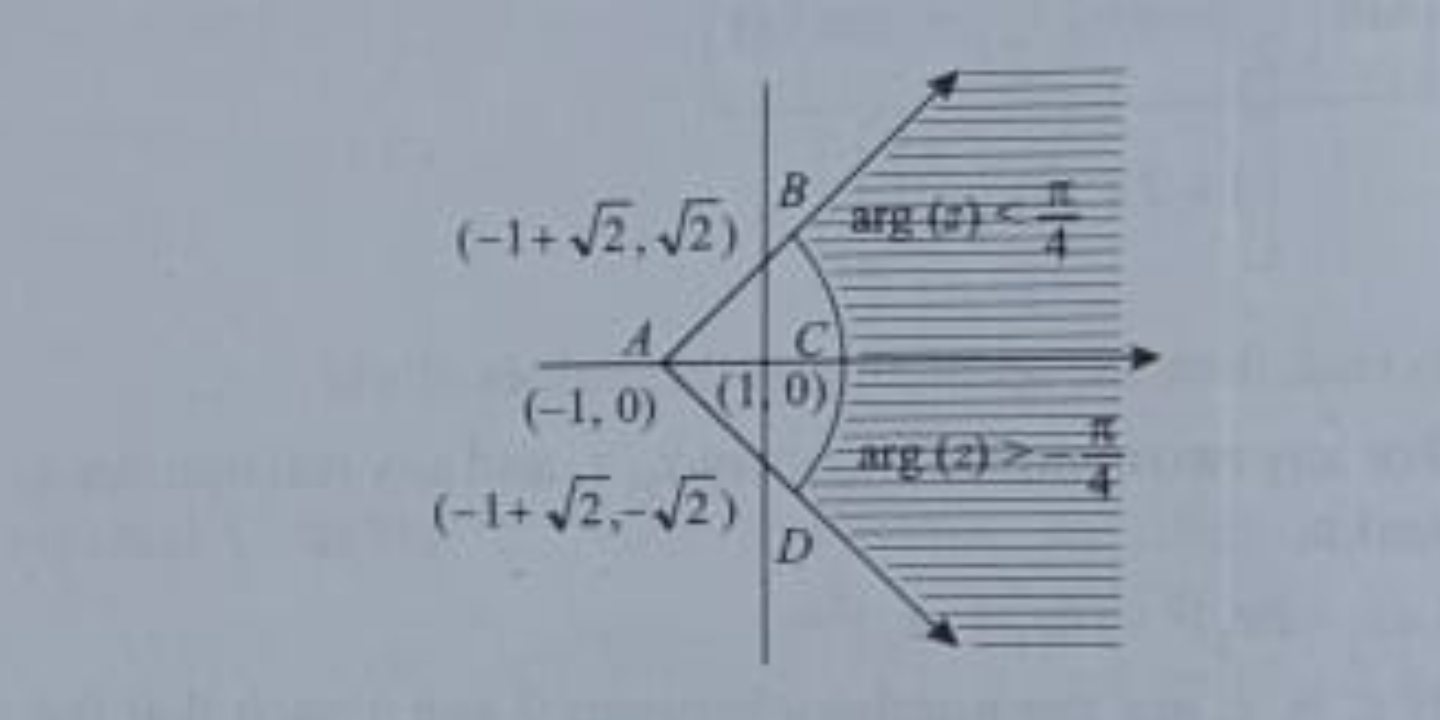
\includegraphics[width=\columnwidth]{./complex/figs/sam.eps}
    \begin{enumerate}
    \item  z:$\abs{ z+1 } > 2$ and $\abs{arg(z+1)} < \pi/4$
    \item   z:$\abs{ z-1} > 2$ and $\abs{ arg(z-1)} < \pi/2$
    \item   z:$\abs{z+1} < 2$ and $\abs{ arg(z+1)} < \pi/4$
    \item   z:$\abs{ z-1} < 2$ and $\abs{ arg(z+1) } < \pi/2$
    \end{enumerate}
    \item a,b,c are integers, not all simultaneously equal and $\omega$ is cube root of unity $(\omega \neq 1)$, then minimum value of $\abs{ a+bw+cw^2} $ is
    \begin{enumerate}
    \item   0
    \item   1
    \item   $\frac{\sqrt3}{2}$
    \item   $\frac{1}{2}$
    \end{enumerate}
    \item Let $w = \frac{-1}{2} + i\frac{\sqrt3}{2}$, then the value of det.
    \\ \myvec{1 & 1 & 1 \\ 1 & -1-\omega^2 & \omega^2 \\ 1 & \omega^2 &\omega^4} is 
    \begin{enumerate}
    \item   $3\omega$
    \item   $3\omega(\omega-1)$
    \item   $3\omega^2$
    \item  $3\omega(1-\omega)$ 
    \end{enumerate}
    \item If $[\frac{w-\bar w z}{1-z}]$ is purely real where $w = \alpha+i\beta$, $\beta \neq 0$ and $z \neq 1$, then the set of the values of z is 
    \begin{enumerate}
    \item   $\{z:\abs z =1\}$
    \item   $\{z:z=\bar z\}$
    \item   $\{z:z\neq1\}$
    \item   $\{z:\abs z=1,z \neq 1\}$
    \end{enumerate}    
    \item A man walks a distance of 3 units from the origin towards the north-east(N 45 degree E) direction. From there, he walks a distance of 4 units toward the north-west(N 45 degree W) direction to each point P. Then the position of P in the Argand plane is
    \begin{enumerate}
    \item   $3e^i\frac{\pi}{4}+4i$ 
    \item   $(3-4i)e^i\frac{\pi}{4}$
    \item   $(4+3i)e^i\frac{\pi}{4}$
    \item   $(3+4i)e^i\frac{\pi}{4}$
    \end{enumerate}
    \item If $\abs z = 1$ and $\abs z \neq 1$ then all the values of $[\frac{z}{1-z^2}]$ lie on 
    \begin{enumerate}
    \item   a line not passing through the origin 
    \item   $\abs z=\sqrt 2$
    \item   the x-axis
    \item   the y-axis    
    \end{enumerate}     
    \item  A particle P starts from point $z_0 = 1+2i$, where $i = \sqrt {-1}$. It moves horizontally away from the origin by 5 units and them vertically away from origin by 3 units to reach a point $z_1$. From $z_1$ is the particle moves $\sqrt{2}$ units in the direction of the vector i+j and then it moves through an angle $\frac{\pi}{2}$ in anticlockwise direction on a circle which centre at origin, to reach a point $z_2$. The point $z_2$ is given by
    \begin{enumerate}  
    \item   $6+7i$ 
    \item   $-7+6i$
    \item   $7+6i$
    \item   $-6+7i$
    \end{enumerate}
    \item Let z = $\cos\theta+i\sin\theta.$ Then the value of $\sum_{m=1}^{15}Im(z^2m-1)$
    at $\theta = 2\degree$ 
    \begin{enumerate}
    \item   $\frac{1}{sin 2 \degree }$ 
    \item   $\frac{1}{3sin 2 \degree }$
    \item   $\frac{1}{2sin 2 \degree }$    
    \item   $\frac{1}{4sin 2 \degree }$
    \end{enumerate}
    \item Let $z = x+iy$ be a complex number where x and y are integers.Then find the area of the rectangle whose vertices are the roots of the equation : $zz^{-3} + \bar z z ^3 = 350$ 
    \begin{enumerate}
    \item 48
    \item 32
    \item 40
    \item 80
    \end{enumerate}    
    \item Let $z$ be a complex numbers such that the imaginary part of $z$ is non-zero and $a = a^2+z+1$ is real. Then a cannot take the value
    \begin{enumerate}        
    \item   $-1$ 
    \item   $\frac{1}{3}$
    \item   $\frac{1}{2}$
    \item   $\frac{3}{4}$
    \end{enumerate}
    \item Let complex numbers $\alpha$ and $\frac{1}{\alpha}$  lie on circles $(x-x_0)^2+(y-y_0)^2\equiv r^2$ and $(x-x_0)^2 (y-y_0)^2\equiv 4r^2$ respectively. If $z_0\equiv x_0+iy_0$ satisfies the equation $2\abs {z_0} ^2 = r^2+2$,then $\abs{\alpha} $=
    \begin{enumerate}
    \item    $\frac{1}{\sqrt 2}$ 
    \item   $\frac{1}{2}$
    \item   $\frac{1}{\sqrt7}$
    \item   $\frac{1}{3}$
    \end{enumerate}
    \item Let S be the set off all complex numbers z satisfying  $\abs z-2+i \geq \sqrt 5$. If the complex numbers $z_0$ is such that ${\abs{\frac{1}{z_0-1}}}$ is the maximum of the set $\{{\vert\frac{1}{z-1}\vert}:z\in S\}$, then the principle argument of $\frac{4-z_0-\bar z_0}{z_0-\bar z_0+2i}$ is 
    \begin{enumerate}
    \item    $\frac{\pi}{4}$ 
    \item   $\frac{3\pi}{4}$
    \item   $\frac{\pi}{2}$
    \item   $\frac{-\pi}{2}$ 
    \end{enumerate}
    \item $z_1 = a+ib$ and $z_2 = c+id$  are complex numbers such that $\abs {z_1} = \abs {z_2}$ = 1 and Re$(z_1 \bar z_2)=0$,then the piar of complex numbers $w_1=a+ic$ and $w_2=b+id$ satisfies 
    \begin{enumerate}
    \item    $\abs w_1 $=1 
    \item   $\abs w_1 $=2
    \item   Re$(w_1 \bar w_2)=0$
    \item   none of these
    \end{enumerate}
    \item Let $z_1$ and $z_2$ be complex numbers such that $z_1\neq z_2$ and  $\abs {z_1} = \abs {z_2} $. If $z_1$ has positive real part and $z_2$ has negative imaginary part,then  $\frac{z_1+z_2}{z_1-z_2}$ may be
    \begin{enumerate}
    \item    zero
    \item   real and positive
    \item   real and negative    
    \item   purely imaginary  
    \item none of these
    \end{enumerate}
    \item If $z_1$ and $z_2$ are two non zero complex numbers such that $\abs{z_1+z_2}$ = $\abs{z_1+ z_2}$, then Arg $z_1$- Arg $z_2$ is equal to
    \begin{enumerate}
    \item    $-\pi$ 
    \item   $\frac{-\pi}{2}$
    \item   $0$    
    \item  $\frac{\pi}{2}$
    \end{enumerate}
    \item The value of $\sum_{k=1}^{6}$ ($\sin\frac{2\pi k}{7}-i\cos\frac{2\pi k}{7}$) is 
    \begin{enumerate}
    \item    $-1$ 
    \item    $0$
    \item   $-i$    
    \item   $i$  
    \item None
    \end{enumerate}
    \item If $\omega$ is an imaginary cube root of unity, then $(1+\omega-\omega^2)^7$ equals 
    \begin{enumerate}
    \item    $128w$ 
    \item    $-128\omega$
    \item   $128\omega^2$    
    \item   $-128\omega^2$
    \end{enumerate}
    \item The value of the sum $\sum_{n=1}^{13}(i^n+i^n+1)$, where $i = \sqrt -1$, equals
    \begin{enumerate}
    \item   $i$ 
    \item   $i-1$
    \item   $-i$    
    \item   $0$
    \end{enumerate}
    \item If $\begin{vmatrix}
    6i &-3i& 1\\ 4&3i&-1 \\20&3&i    \end{vmatrix}$ = x+iy,then 
    \begin{enumerate}
    \item   $x=3,y=2$ 
    \item   $x=1,y=3$
    \item   $x=0,y=3$    
    \item  $x=0,y=0$
    \end{enumerate}
    \item Let $z_1$ and $z_2$ be two distinct complex numbers and let $z=(1-t)z_1+tz_2$ for real some numbers t with $0 < t < 1$.If Arg(w) denotes the principle argument of a non-zero complex number w then 
    \begin{enumerate}
    \item   $\vert z-z_1 \vert+\vert z-z_2 \vert=\vert z_1-z_2 \vert$ 
    \item   $Arg(z-z_1)=Arg(z-z_2)$
    \item   $ \myvec{z-z_1 & \bar z-\bar z_1 \\ z_2-z_1 & \bar z_2-\bar z_1}$         
    \item  $Arg(z-z_1)=Arg(z_2-z_1)$
    \end{enumerate}
    \item Let 
    $w = \frac{\sqrt{3+i}}{2}$ and 
    $P = {w^n:n=1, 2, 3,......}$. Further $H_1 = { z\in C: Rez>\frac{1}{2}}$ and 
    $H_2={ z\in C: Rez<\frac{-1}{2}}$,where c is the set of all complex numbers. 
    If $Z_1 I P C H_1,z_2 I P c H_2$ and O represents the origin. then $\angle z_1 o z_2 =$
    \begin{enumerate}
    \item  $\frac{p}{2}$ 
    \item  $\frac{p}{6}$
    \item  $\frac{2p}{3}$
    \item  $\frac{5p}{6}$
    \end{enumerate}
    \item Let $a,b,c\in R$ and $a^2+b^2\neq = 0$ 
    suppose $S = {Z \in C:Z=\frac{1}{a+ibt},+ \in R,t \neq0}$,where $i = \sqrt-1$.If $z = x+iy$ and $z\in S $,then $\myvec(x,y)$ lies on
    \begin{enumerate}
    \item the circle with radius $\frac{1}{2a}$ and centre $[ \,\frac{1}{2a},0] \,$ for $agr > 0,$	 
    \item  the circle with radius $\frac{-1}{2a}$ and centre $[ \,\frac{-1}{2a},0] \,$ for $a < 0, b\neq 0$
    \item  the x-axis for a $a\neq 0,b=0$
    \item   the x-axis for a $a=0,b\neq 0$
    \end{enumerate}
    \item Let a, b x and y real numbers such that $a-b=1$ and $y\neq 0$. If the complex number $z=x+iy$ satisfies $Im[\frac {az+b}{z+1}] = y$ then which of the following  is(are) possible values(s) of X ?
    \begin{enumerate}
    \item   $-1+\sqrt1-y^2$ 
    \item   $-1-\sqrt1-y^2$
    \item   $1+\sqrt1+y^2$ 
    \item   $1-\sqrt1+y^2$
    \end{enumerate}
    \item For a non-zero complex numbers z let arg(z) denote the principle argument with $-\pi < arg(z)\leq\pi$.Then which of the following statement(s) is(are) $\boldsymbol{FALSE} ?$
    \begin{enumerate}
    \item   $arg(-1-i)=\frac{\pi}{4}$, where $i=\sqrt -1$ 
    \item   the function $ f :R \longrightarrow(-\pi.\pi] \,$, defined by $f(t)=arg(-1+it)$ for all $\in R$, is continues at all points of R, where $i=\sqrt-1$ 
    \item  For any two non-zero complex numbers $z_1$ and $z_2$,
     arg$[ \,\frac{z_1}{z_2}] \,-arg(z_1)+arg(z_2)$ is an integer multiple of $2\pi$
    \item  Foe any three given distinct complex numbers $z_1$, $z_2$ and $z_3$, the locus of the point z satisfying the condition 
         $arg[ \,\frac{(z-z_1)(z_2-z_3)}{(z-z_3)(z_2-z_1)}] \,$=$\pi$,lies on a straight line
    \end{enumerate}
    \item Let s,t,r be non-zero complex numbers and L be the set od solutions $z = x+iy(x,y \in R,
    i = \sqrt -1)$ of the equation $sz+t\bar z+r$ = 0, where $\bar z = x-iy$.Then , which of the following statements(s) is (are) TRUE ?
    \begin{enumerate}
    \item   If L has exactly on element , then $\abs s \neq \abs t $
    \item   If $\abs s = \abs t $, then L has infinitely many elements 
    \item   the number of elements in $L\cap { z :\vert z-1+i\vert =5}$ is at most 2
    \item   If L has a more than on element,then L has infinitely many elements
    \end{enumerate}
    \item Express $\frac{1}{1-cos\theta+2isin\theta}$ in the for, of $x+iy$
    \item If $x = a+b,y = a\gamma+b\beta$ and $z = a\beta+b\gamma$ where $\gamma$ and $\beta$ are the complex cube roots of unity, Show that $xyz=a^3+b^3$.
    \item If $x+iy = \sqrt{\frac{a+ib}{c+id}}$,prove that $(x^2+y^2)^2 = \frac{a^2+b^2}{c^2+d^2}$
    \item Find the real values of x and y for which the following equation is satisfied $\frac{(1+i)x-2i}{3+i}$+$\frac{(2-3i)y+i}{3-i} = i$
    \item Let the complex numbers $z_1$,$z_2$ and $z_3$ be the vertices of an equilateral traingle.Let $z_0$ be the circumcentre of the the triangle. Then prove that $z_1^2+z_2^2+z_3^2 = 3z_0^2$.
    \item Prove that the complex numbers $z_1,z_2$ and the origin form an equilateral triangle only if
    $z_1^2+z_2^2-z_1z_2 = 0$.
    \item If 1, a,$a_1,a_2........a_n-1$ are the n roots of unity ,then show that $(1-a_1)(1-a_2)(1-a_3).............(1-a_{n-1}) = n$
    \item Show that the area of triangle on the Argand diagram formed by the complex numbers $z, iz$ and $z+iz$ is $\frac{1}{2}\abs{z}^2$.
    \item Let $z-1 = 10+6i$ and $z_1 = 4+6i$.If Z is any complex number
    such that the argument of $\frac{(Z-Z_1)}{(Z-Z_2)}$ is $\frac{\pi}{4}$, then prove that $\abs{ z-7-9i} =3\sqrt 2$.
    \item  If $iz^3-z^2+z+i = 0$, then show that  $\abs z = 1$
    \item If $\abs Z \leq 1, \abs W \leq 1$ show that 
    $\abs Z-W^2 \leq (\abs Z -\abs W )^2+(ArgZ-ArgW)^2$
    \item Find all non-zero complex numbers $Z$ satisfying $\bar Z = iZ^2$.
    \item Let $z_1$ and $z_2$ be roots of the equation $x^2+pz+q = 0$,where the coefficients $p$ and $q$ may be complex numbers.Let A and B represents $z_1$ and $z_2$ in the complex plane.If $\angle AOB = \alpha \neq 0$ and $OA=OB$, where $O$ is the origin, prove that
    $p^2=4qcos^2 (\frac{\alpha}{2})$
    \item For complex numbers $z$ and $w$, prove that $\abs z ^2 w - \abs w^2 z=z-w$ if and only if $z=w$ or  $z\bar z=1$
    \item Let a complex number $\alpha$,$\alpha \neq 1$, be a rot of root of the equation $z^p+q-z^p-z^q+1 = 0$,where p,q are distinct primes. Show that either $a+\alpha+\alpha^2+..........\alpha^p-1$ or $a+\alpha+\alpha^2+..........\alpha^q-1 = 0$, but not the together.
    \item If $z_1$ and $z_2$ are two complex numbers such that $\abs{ z_1} < 1 < \abs {z_1}$ then prove that $\abs {\frac {1-z_1\bar z_2}{z_1-z_2}} < 1$. 
    \item Prove that there exists no complex number z such that $\abs z <\frac{1}{3}$ and $\sum_{r=1}^{n}a_r z ^r=1$ where $\abs a_r <2$.
    \item Find the centre and radius of circle given by 
    $\abs{\frac{z-\alpha}{z-\beta}}$ = k,k$\neq$ 1
    where,z=i+xy, $\alpha = \alpha_1+i \alpha_2,\beta = \beta_1+i \beta_2$
    \item If one of the vertices of the square circumscribing the circle $\abs {z-1}=\sqrt 2$ is $2+\sqrt{3}$i.Find the other vertices of the square.
{\textbf{PASSAGE-1}}\\
Let A,B,C be three sets of complex numbers as defined below 
    $A=\{z:Im z\leq 1\}$\\*
    $B=\{z:\abs{ z-2-i}=3\}$\\*
    $C=\{z:Re((1-i)z)=\sqrt 2\}$
    \item The number of elements in the set $A\cap B \cap C$ is 
    \begin{enumerate}
    \item (a) 0   
    \item (b) 1   
    \item (c) 2   
    \item (d) $\infty$
    \end{enumerate}
    \item Let z be an any point in $A\cap B \cap C$.
    Then, $\abs{z+1-i}^2+\abs{z-5-i}^2$ lies between
    \begin{enumerate}
    \item (a) 25 and 29   
    \item (b) 30 and 44    
    \item (c) 35 and 39    
    \item (d) 40 and 44
    \end{enumerate}
    \item Let z be any point $A\cap B \cap C$ and let w be any point satisfying $w-2-i < 3$. Then $\abs z -\abs w +3$ lies between     
    \begin{enumerate}
    \item (a) -6 and 3    
    \item (b)  -3 and 6    
    \item (c)  -6 and 6    
    \item (d)  -3 and 9
\end{enumerate}
\textbf{PASSAGE-2}
Let $S = S_1\cap S_2\cap S_3$\\
where $S_1 = \{z\in C : \abs z < 4\},$\\
$S_2 = \{z \in C:m[\frac{z-1+\sqrt{31}}{1-\sqrt{31}}>0]\}$ and \\ 
$S_3 = \{z \in C :Rez>0\}.$
	\item Area of S=
    \begin{enumerate}
    \item (a) $\frac{10\pi}{3}$    
    \item (b) $\frac{20\pi}{3}$    
    \item (c) $\frac{16\pi}{3}$    
    \item (d) $\frac{32\pi}{3}$
    \end{enumerate}
    \item $min_z \in_S\abs1-3i-z=$
    \begin{enumerate}
    \item (a) $\frac{2-\sqrt 3}{2}$    
    \item (b) $\frac{2+\sqrt 3}{2}$    
    \item (c) $\frac{3-\sqrt 3}{2}$    
    \item $\frac{3+\sqrt 3}{2}$
    \end{enumerate} 
        \item If z is any complex number satisfying  $\abs{z-3-2i} \leq 2$,then the minimum value of 
        $\abs{ 2z=6+5i}$ is
        \item Let $\omega = e^\frac{i\pi}{3}$, and a,b,c,x,y,z be non-zero complex numbers such that 
        $a+b+c = x$
        $a+b\omega+c\omega^2 = y$
        $a+b\omega^2+c\omega = z$
        Then the value of $\frac{\abs x^2+\abs y^2+\abs z ^2}{\abs a^2+\abs b^2 +\abs c^2}$ is 
        \item For any integer k, let $\alpha_k = \cos(\frac{k\pi}{7})+isin(\frac{k\pi}{7})$,where
        $i=\sqrt-1$.The value of the expression  $\frac{\sum{k=1}^{12}\abs\alpha_k+1-\alpha_k}{\abs{\sum_{k=1}^{3}\alpha_4k-1-\alpha_4k-2}}$ is
        \item Let $\omega \neq 1$ be a cube root of unity. Then the minimum value  of the set {${\abs{a+b\omega+c\omega^2}^2:}$} a,b,c distinct non-zero integers .......
    \item z and w are two nonzero complex numbers such that $\abs z = \abs w$ and Argz+Argw = $\pi$ then z equals
    \begin{enumerate}
    \item  $\bar{\mathbb{\omega}}$
    \item  $\bar{\mathbb{-\omega}}$
    \item  ${\omega}$
    \item  $\bar{-\omega}$
    \end{enumerate}
    \item If $\abs z-4<\abs x-2$ ,its solution is given by     
    \begin{enumerate}
    \item  Re(z) $>$ 2
    \item  Re(z) $<$ 2
    \item Re(z) $>$ 3
    \item  Re(z)$<$ 2
    \end{enumerate}
    \item The locus of the centre of a circle which touches the cirlce $\abs{z-z_1} = a$ and $\abs{z-z_2} = b$ externally        
    ($z,z_1$ and $z_2$ are complex numbers) will be 
    \begin{enumerate}
    \item  an ellipse
    \item  a hyperbola    
    \item  a cirlce
    \item  none of these
    \end{enumerate}
    \item If z and $\omega$ are two non-zero complex numbers such that $\abs z\omega $ = 1 and Arg(z)-Arg($\omega$) = $\frac{\pi}{2}$, then $\bar{z}\omega$ is equals to 
    \begin{enumerate}
    \item  -i
    \item  1    
    \item  -1
    \item  i
    \end{enumerate}
    \item Let $Z_1$ and $Z_2$ be two roots of the equation \\
    $Z^2+aZ+b = 0$, Z being complex. Further, assume that the origin $Z_1$ and $Z_2$ form an equilateral triangle.Then
    \begin{enumerate}
    \item  $a^2$ = 4b
    \item  $a^2$ = b    
    \item  $a^2$ = 2b
    \item  $a^2$ = 3b
    \end{enumerate}
    \item If $({\frac{1+i}{1-i}})^x = 1$ then 
    \begin{enumerate}
    \item  x=2n+1,Where n is any positive integer
    \item  x=4n,Where n is any positive integer    
    \item  x=2n,Where n is any positive integer
    \item x=4n+1,Where n is any positive integer
    \end{enumerate}
    \item Let z and w be complex numbers such that $\bar{z}+i\bar{{w}}$ = 0 and arg zw = $\pi$, Then arg z equals
    \begin{enumerate}
    \item  $\frac{5\pi}{4}$
    \item  $\frac{\pi}{2}$    
    \item  $\frac{3\pi}{4}$    
    \item  $\frac{\pi}{4}$
    \end{enumerate}
    \item If z=x-iy and $z^\frac{1}{3}$=p+iq, then $( \frac {x}{p}+\frac{y}{p})/(p^2+q^2)$ is equal to
    \begin{enumerate}
    \item  -2
    \item  -1    
    \item  2
    \item  1
    \end{enumerate}
    \item If $abs z^2-1=\abs z ^2+1$, then z lies on
    \begin{enumerate}
    \item  an ellipse
    \item  the imaginary axis    
    \item  a circle
    \item  the real axis
    \end{enumerate}
 \item If the cube roots of unity are 1, 1, $\omega, \omega^2$ then the roots of the equation $(x-1)^3+8 = 0$ are 
    \begin{enumerate}
    \item  -1,-1+2w,$s-1-2w^2$
    \item  -1,-1,-1    
    \item  -1,1-2w,$1-2w^2$
    \item  -1,1+2w,$1+2w^2$
    \end{enumerate}
    \item If $Z_1$ and $z_2$  are two non-zero complex numbers such that $\abs z_1 + z_2 = \abs z_1+ z_2$, then arg $z_1$-arg$z_2$ is equal to
    \begin{enumerate}
    \item  $\frac{\pi}{2}$    
    \item  $-\pi$    
    \item  0
    \item  $-\frac{\pi}{2}$
    \end{enumerate}
    \item If $\omega = \frac{z}{z-\frac{1}{3i}}$ and $\abs \omega = 1$, then z lies on 
    \begin{enumerate}
    \item  an ellipse    
    \item  a circle    
    \item  a straight line
    \item  a parabola
    \end{enumerate}
    \item The value of $\sum_{n=1}^{10}(\sin\frac{2k\pi}{11}+i\cos\frac{2k\pi}{11})$ is 
    \begin{enumerate}
    \item  $i$    
    \item  $1$    
    \item  $-1$
    \item  $-i$    
    \end{enumerate}
    \item $z^2$+z+1 = 0, Where Z is complex number, then the value of
    $( z+\frac{1}{z})^2$ + $( z^2+\frac{1}{z^2})^2$ + $( \,z^3+\frac{1}{z^3}\,)^2$+..........$( \,z^6+\frac{1}{z^6}\,)^2$ is
    \begin{enumerate}
    \item  18    
    \item  54    
    \item  6
    \item  12
    \end{enumerate}
    \item If $\abs{z+4 \leq 3}$, then the maximum value of  $\abs z+1 $ is 
    \begin{enumerate}
    \item  6    
    \item  0    
    \item  4
    \item 10
    \end{enumerate}
    \item The conjugate of a complex number is $abs{ \frac{-1}{i-1}}$ then that complex  number is 
    \begin{enumerate}
    \item  $\frac{-1}{i-1}$    
    \item  $\frac{11}{i+1}$    
    \item  $\frac{-1}{i+1}$
    \item  $\frac{1}{i-1}$
    \end{enumerate}
    \item  Let R be the real line. consider the following subsets of the plane $ R \times  R$:
    $S=\{(x,y):y=x+1$ and $0 < x < 2 \}$
    $T=\{(x,y):x-y is an integer\}$,
    Which on of the following is true?
    \begin{enumerate}
    \item  Neither S or T is an equivalence relation of R    
    \item  Both S and T are equivalence relation of R    
    \item  S is an equivalence relation on R but T is not
    \item  T is an equivalence relation on R but S is not
    \end{enumerate}
     \item The number of complex numbers z such that\\
    $\abs{ z-1}$=$\abs{ z+1}$=$\abs{z-i}$ equals
    \begin{enumerate}
    \item  $1$    
    \item  $2$    
    \item  $\infty$
    \item  $0$
    \end{enumerate}
    \item Let $\alpha$, $\beta$ be a real and z be a complex numbers, If $z^2+\alpha z +\beta$=0  has two distinct roots on the line Re z =1, then it is necessary that:
    \begin{enumerate}
    \item  $\beta \in (-1,0)$    
    \item  $\abs{\beta} $=1    
    \item  $\beta \in (1,\infty)$
    \item  $\beta \in (0,1)$
    \end{enumerate}
    \item If $\omega(\neq)1$ is a cube root of unity, and $(1+\omega)^2 = A+B\omega$. Then (A,B) equals
    \begin{enumerate}
    \item  $(1,1)$    
    \item  $(1,0)$    
    \item  $(-1,1)$
    \item  $(0,1)$
    \end{enumerate}
    \item If $z \neq 1$ and $\frac{z^2}{z-1}$ is real, then the point represented by the complex numbers z lies:
    \begin{enumerate}
    \item  either on the real axis or on a circle passing through the origin.
    \item  on a circle with centre  at the origin    
    \item  either on the real axis or on a circle not passing through  the origin.
    \item  on the imaginary axis.
    \end{enumerate}
    \item If z is a complex number of unit modulus and argument $\theta$, then $arg\frac{1+z}{1+\bar z}$ equals:
    \begin{enumerate}
    \item  $-\theta$    
    \item  $(\frac{\pi}{2}-\theta)$    
    \item  $\theta$
    \item  $\pi-\theta$
    \end{enumerate}
    \item If z is a complex number such that $\abs {z} \geq2$, then the minimum
    value of $\abs{ z+ \frac{1}{2}}$:
    \begin{enumerate}
    \item  is strictly greater than $\frac{5}{2}$    
    \item  is strictly greater than $\frac{3}{2}$ but less than $\frac {5}{2}$    
    \item  is equal to $\frac {5}{2}$
    \item  lie in the interval $(1,2)$
    \end{enumerate}
     \item A complex number z is said to be uni modular if $\abs {z}$ = 1.Suppose $z_1$ and $z_2$ are complex number such that $\frac{z_1-2z_1}{2-z_1\bar z_2}$ is uni modular and $z_2$ is not uni modular. Then the point $z-1$ lies on a:
    \begin{enumerate}
    \item  circle of radius $2$.    
    \item  circle of radius $\sqrt 2$    
    \item  straight line parallel to x-axis
    \item  straight line parallel to y-axis
    \end{enumerate}
    \item  A value of $\theta$ for which $\frac{2+3i\sin\theta}{1-2i\sin\theta}$ is purely  imaginary,is 
    \begin{enumerate}
    \item  $sin^-1(\frac {\sqrt 3}{4})$    
    \item  $sin^-1(\frac {1}{\sqrt 3})$    
    \item  $\frac{\pi}{3}$
    \item  $\frac{\pi}{6}$
    \end{enumerate}
    \item Let $A = \{\theta \in (\frac{\pi}{2},\pi):\frac {3+2i\sin\theta}{1-2i\sin\theta }$is purely imaginary. Then the sum of elements in A is
    \begin{enumerate}
    \item  $\frac{5\pi}{6}$   
    \item  $\pi$    
    \item  $\frac{3\pi}{4}$
    \item  $\frac{2\pi}{3}$
    \end{enumerate}
    \item Let $\alpha$ and $\beta$ be two roots of the equation $x^2+2x+2$ = 0, then $\alpha^15+\beta^15$ is equal to:
    \begin{enumerate}
    \item  $-256$    
    \item  $512$    
    \item  $-512$
    \item  $256$
    \end{enumerate}
    \item All the points in the set 
    $S=\{\frac{\alpha+i}{\alpha-i}:\alpha \in R\}i = \sqrt -1$ lie on  :
    \begin{enumerate}
    \item  straight line whose slope is 1.    
    \item  circle whose radius is 1.    
    \item  circle whose radius is $sqrt 2$.
    \item  straight line whose slope is -1.
    \end{enumerate}
    \onecolumn
    {\textbf{Match the following }}\\
{\textbf{DIRECTIONS(Q-1):}}{Each question contains statements given in two columns,which have to be matched.The statement in Column-I are labelled A,B,C and D, while the statements in Column-II are labelled p,q,r,s and t.Any given statement in Column-I can have correct matching with ONE OR MORE statement(s) in Column-II.The appropriate bubbles corresponding to the answers to these questions have to be darkened as illustrated in the following example:}\\*
%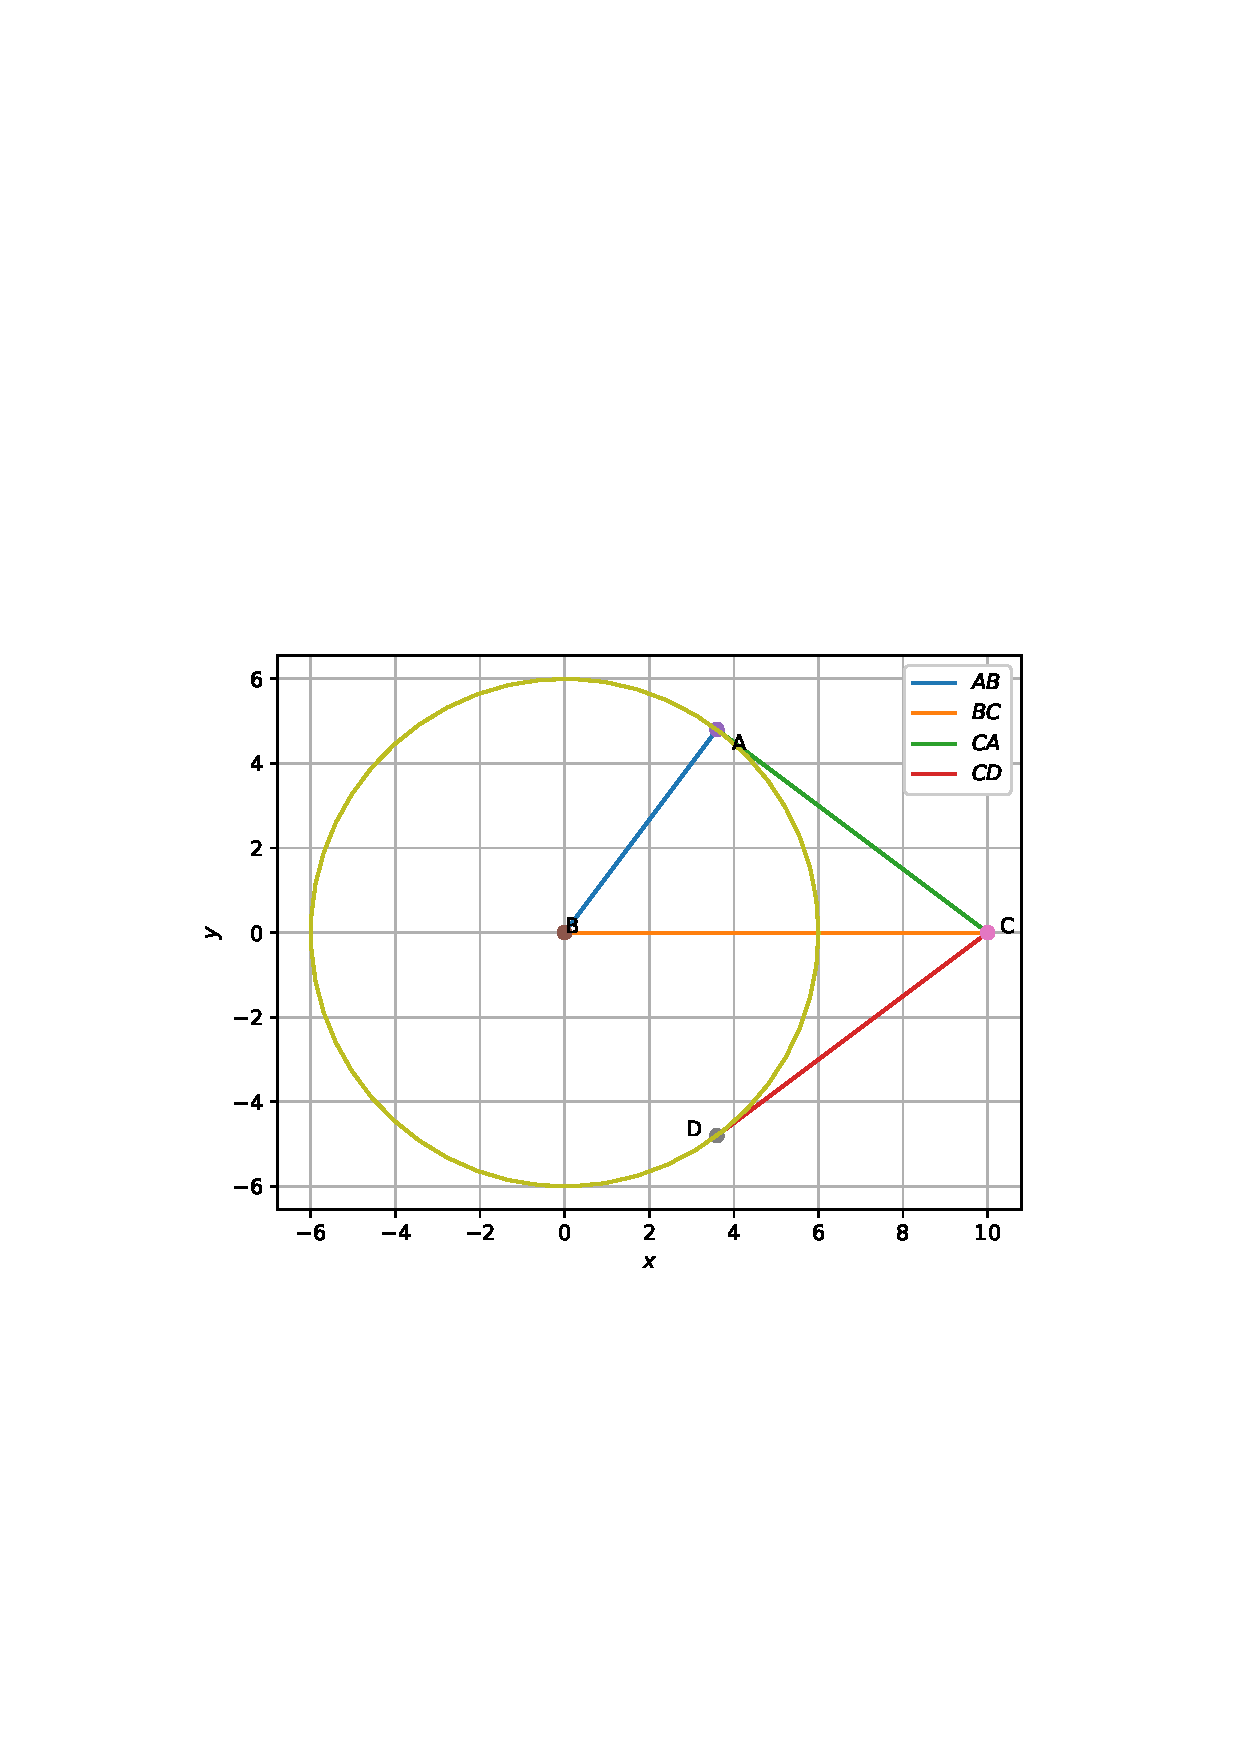
\includegraphics[scale=0.4]{circle.jpg} \\*
If the correct matches are A-p,s and t;B-q and r; C-p and q and D-s then the correct darkening of bubbles will look like the given.
\item z$\neq$ 0 is a complex number\\
\begin{tabular}{llll}
\textbf{Column-I} &   \enspace   &   \textbf{Column-II}\\
(A) $Rez=0$ &   \enspace  &   (p)$Rez^2=0$\\
&&&\\
(B) $Argz=\frac{\pi}{4}$    &   \enspace   & (q)$Imz^2-6$\\
&&&\\
          &\enspace   &   (r)$Imz^2-6$\\
&&&\\
\end{tabular}
\item Match the statements in \textbf{Column-I} with those in \textbf{Column-II}\\
NOTE:Here z takes values in the complex plane and Im z and Re Z denote, respectively,the imaginary part and real part of z
\begin{tabular}{llll}
\textbf{Column-I} &  \enspace   &  \textbf{Column-II}\\
(A) The set of points z satisfying\\
 $\abs {z-iz}=\abs{z+iz} $ is contained in or equal to  &   \enspace   & (p)n ellipse with eccentricity$\frac{4}{5}$\\
&&&\\
(B) The set of all points satisfying \\
$\abs {z+4}+\abs{z-4}=10$ is contained \\
in or equal to   &   \enspace   & (q)the set of points z satisfying  $Imz=0$\\
&&&\\
(C) If $\abs{w}$=2, then the set of points\\
 $z=w-\frac{1}{w}$  &   \enspace  & (r)the set of points z satisfying $\abs{ Im z} \leq 1$\\
&&&\\
(D) If $\abs{ w} =1$, then the set of points\\
    $z=w+\frac{1}{w}$ is contained in or equal to  &   \enspace   & (s) the set of points z satisfying  $Rez\leq 2$\\*
&&&\\
\end{tabular}\\
\clearpage
    \textbf{DIRECTIONS(Q.3)} Following question has matching lists. The codes for the list have choices(a),(b),(c) and (d) out of which ONLY ONE is correct

    \item Let $z_k=cos(\frac{2k\pi}{10})+isin(\frac{2k\pi}{10});k=1,2,3........9$\\*
\begin{tabular}{llll}
\textbf{LIST-I} & \enspace & \textbf{LIST-II}\\&&&\\ 

(P) For each $z_k=$ there exists as \\
$z_j$ such that $z_k,z_j=1$ &   \enspace   &   (1)Trues\\
&&&\\
(Q) There exists a $k\in \{a,2........9\}$ such that\\
 $z_1,z=z_k$ has no solution z in the set of complex numbers    &   \enspace  & (2)False\\
&&&\\
(R) $\frac{\abs{ 1-z_1} 1-z_2...\abs{ 1-z_9}}{10}$ equals   &   \enspace   & (3)1\\    
&&&\\
(S) 1-$\sum_{k=1}^{9}(\frac{2k\pi}{10})$    &   \enspace  & (3)2\\          
&&&\\
\end{tabular}
       \textbf{P}\hspace{5pt}\textbf{Q}\hspace{5pt}\textbf{R}\hspace{5pt}\textbf{S}\\*
    (a) {1}\hspace{5pt}{2}\hspace{5pt}{4}\hspace{5pt}{3}\\*     
    (b) {1}\hspace{5pt}{2}\hspace{5pt}{3}\hspace{5pt}{4}\\*
    (c) {2}\hspace{5pt}{1}\hspace{5pt}{3}\hspace{5pt}{4}\\*
    (d) {2}\hspace{5pt}{1}\hspace{5pt}{4}\hspace{5pt}{3}\\* 
\end{enumerate}
%\end{document}
    
 
\end{document}


